\documentclass[11pt, twoside, fleqn]{article} % use \documentstyle for old LaTeX compilers

\usepackage[ngerman]{babel} % 'french', 'german', 'spanish', 'danish', etc.
\usepackage{float}
\everymath{\displaystyle}
\usepackage{amsmath,nccmath} 
\usepackage{anyfontsize}

% Helvetica = Arial for sections
\usepackage{helvet}
\fontfamily{Name_OF_Font_Family}\selectfont

\usepackage{titlesec}
\titleformat{\section}
  {\fontfamily{phv}\selectfont\Large\bfseries}
  {\thesection}{1em}{}

\usepackage{titlesec}
\titleformat{\subsection}
  {\fontfamily{phv}\selectfont\large\bfseries}
  {\thesubsection}{1em}{}
  
\usepackage{titlesec}
\titleformat{\subsubsection}
  {\fontfamily{phv}\selectfont\bfseries}
  {\thesubsubsection}{1em}{}

\usepackage{amsfonts} 
\usepackage{amssymb}
\usepackage{mathtools}
\usepackage{hyperref}
\usepackage{txfonts}
\usepackage{mathdots}
\usepackage[classicReIm]{kpfonts}
\usepackage[utf8]{inputenc}
\usepackage{graphicx}
\usepackage{biblatex} 
\usepackage{csquotes}
\usepackage{geometry}
\usepackage{siunitx}
\usepackage{subcaption}
\usepackage[export]{adjustbox}
\usepackage{wrapfig}
\usepackage[justification=centering]{caption}


\setlength\mathindent{0pt}
\input{insbox}

% set row height 
\usepackage{stackengine}
\newcommand\xrowht[2][0]{\addstackgap[.5\dimexpr#2\relax]{\vphantom{#1}}}

%\usepackage[scaled=.90]{helvet}% Helvetica, served as a model for arial
\usepackage{titlesec}
 \geometry{
 a4paper,
 total={175mm,257mm},
 left=20mm,
 top=20mm,
 }

% caption set
\usepackage{caption} 
\captionsetup[table]{justification=raggedright,singlelinecheck = false}
\DeclareCaptionFormat{myformat}{\fontfamily{phv}\selectfont#1#2#3\par}
\captionsetup{format=myformat,font=small}

% table set
\usepackage{xcolor,fancyhdr}
\usepackage{array,multirow,colortbl}
\usepackage{multicol}
 
% set fancy header, remove foot number page
\usepackage{fancyhdr}
\pagestyle{fancy}
\fancyhead[LE,RO]{\small\thepage}
\fancyhead[RE]{\small \emph{\nouppercase{\leftmark}}}
\fancyhead[LO]{\small \emph{\nouppercase{\rightmark}}}
\setlength{\headheight}{14pt}
\cfoot{} 

\newcolumntype{C}[1]{>{\centering\arraybackslash }b{#1}}

% Numbering automatically for sections 
\numberwithin{equation}{section}
\numberwithin{table}{section}
\usepackage[tablename=Tabelle]{caption}
\numberwithin{figure}{section}
\usepackage[figurename=Bild]{caption}

% Matlab listing
\usepackage[numbered,framed]{matlab-prettifier}
\usepackage{filecontents}
\let\ph\mlplaceholder % shorter macro
\lstMakeShortInline"

\lstset{
  style              = Matlab-editor,
  basicstyle         = \mlttfamily,
  escapechar         = ",
  mlshowsectionrules = true,
    literate=%
    {Ö}{{\"O}}1
    {Ä}{{\"A}}1
    {Ü}{{\"U}}1
    {ß}{{\ss}}2
    {ü}{{\"u}}1
    {ä}{{\"a}}1
    {ö}{{\"o}}1
}

% Change Inhalt's word
\renewcommand*\contentsname{Inhalt}

\begin{document}
\thispagestyle{empty} % remove the header
\begin{figure}[H]
  \centerline{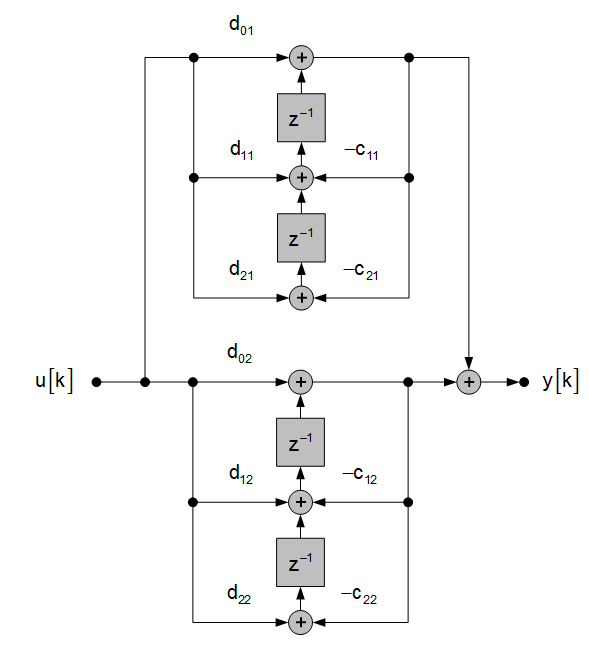
\includegraphics[width=0.6\textwidth]{SignalflussParallelstruktur.png}}
\end{figure}

\noindent \bigskip

\centerline  {\fontfamily{phv}\fontsize{50}{60}\selectfont Systemtheorie Teil B} 

\noindent \medskip

\centerline  {\fontfamily{phv}\fontsize{23}{30}\selectfont  - Zeitdiskrete Signale und Systeme -}

\noindent \bigskip
\noindent \bigskip

\centerline  {\fontfamily{phv}\fontsize{23}{30}\selectfont  Manfred Strohrmann}\medskip

\noindent 

\centerline  {\fontfamily{phv}\fontsize{23}{30}\selectfont Urban Brunner}

\vspace{6.0\baselineskip}

\begin{figure}[H]
  \centerline{
\includegraphics[width=0.6\textwidth]{FH_Logo.png}}
\end{figure}

\clearpage
\newpage

\thispagestyle{empty}
\section*{Änderungsindex}
\begin{table}[H]
\setlength{\arrayrulewidth}{.1em}
\setlength{\fboxsep}{0pt}
\begin{tabular}{wl{1.4cm} | wl{2.3cm} | wl{2.5cm} | wl{9.8cm}}
\xrowht{15pt}

\fontfamily{phv}\selectfont\textbf{Version} &
\fontfamily{phv}\selectfont\textbf{Datum} & 
\fontfamily{phv}\selectfont\textbf{Verfasser} & 
\fontfamily{phv}\selectfont\textbf{Änderungen}\\ \hline \xrowht{15pt}

\multirow{2}{*}{\fontfamily{phv}\selectfont{10}} &
\multirow{2}{*}{\fontfamily{phv}\selectfont{15.08.2020}} &
\fontfamily{phv}\selectfont{M. Strohrmann,} &
\fontfamily{phv}\selectfont{Fehlerkorrektur, Ausgabe für Vorlesung}\\ \xrowht{10pt}

&
&
\fontfamily{phv}\selectfont{U. Brunner} &
\fontfamily{phv}\selectfont{WS 2020/21}\\ \hline \xrowht{15pt}

\multirow{2}{*}{\fontfamily{phv}\selectfont{9}} &
\multirow{2}{*}{\fontfamily{phv}\selectfont{15.09.2015}} &
\fontfamily{phv}\selectfont{M. Strohrmann,} &
\fontfamily{phv}\selectfont{Fehlerkorrektur, Ausgabe für Vorlesung}\\ \xrowht{10pt}

&
&
\fontfamily{phv}\selectfont{U. Brunner} &
\fontfamily{phv}\selectfont{WS 2017/18}\\ \hline \xrowht{15pt}

\multirow{2}{*}{\fontfamily{phv}\selectfont{8}} &
\multirow{2}{*}{\fontfamily{phv}\selectfont{15.09.2015}} &
\fontfamily{phv}\selectfont{M. Strohrmann,} &
\fontfamily{phv}\selectfont{Fehlerkorrektur, Ausgabe für Vorlesung}\\ \xrowht{10pt}

&
&
\fontfamily{phv}\selectfont{U. Brunner} &
\fontfamily{phv}\selectfont{WS 2015/16}\\ \hline \xrowht{8pt}

\multirow{3}{*}{\fontfamily{phv}\selectfont{7}} &
\multirow{3}{*}{\fontfamily{phv}\selectfont{15.03.2015}} &
\multirow{2}{*}{\fontfamily{phv}\selectfont{M. Strohrmann,}} &
\fontfamily{phv}\selectfont{Trennung von Text, Übungsaufgaben und Musterlösungen,}\\ \xrowht{8pt}

&
&
\multirow{2}{*}{\fontfamily{phv}\selectfont{U. Brunner}} &
\fontfamily{phv}\selectfont{Überarbeitung Kapitel 11: Diskrete Fourier Transformation,}\\ \xrowht{8pt}

&
&
&
\fontfamily{phv}\selectfont{Ausgabe für Vorlesung SS 2015}\\ \hline \xrowht{15pt}

\multirow{2}{*}{\fontfamily{phv}\selectfont{6}} &
\multirow{2}{*}{\fontfamily{phv}\selectfont{15.03.2014}} &
\fontfamily{phv}\selectfont{M. Strohrmann,} &
\fontfamily{phv}\selectfont{Integration der Systemtheorie Online Funktionen,}\\ \xrowht{10pt}

&
&
\fontfamily{phv}\selectfont{U. Brunner} &
\fontfamily{phv}\selectfont{Korrektur von Fehlern und Überarbeitung}\\ \hline \xrowht{15pt}

\fontfamily{phv}\selectfont{5} &
\fontfamily{phv}\selectfont{14.03.2012} &
\fontfamily{phv}\selectfont{M. Strohrmann} &
\fontfamily{phv}\selectfont{Korrektur von Fehlern und Überarbeitung}\\ \hline \xrowht{15pt}

\multirow{2}{*}{\fontfamily{phv}\selectfont{4}} &
\multirow{2}{*}{\fontfamily{phv}\selectfont{14.03.2014}} &
\multirow{2}{*}{\fontfamily{phv}\selectfont{M. Strohrmann}} &
\fontfamily{phv}\selectfont{Kapitel 10: Strukturen digitaler Systeme}\\ \xrowht{10pt}

&
&
&
\fontfamily{phv}\selectfont{Korrektur von Fehlern und Überarbeitung}\\ \hline \xrowht{15pt}

\fontfamily{phv}\selectfont{3} &
\fontfamily{phv}\selectfont{14.03.2011} &
\fontfamily{phv}\selectfont{M. Strohrmann} &
\fontfamily{phv}\selectfont{Korrektur von Fehlern und Überarbeitung}\\ \hline \xrowht{15pt}

\fontfamily{phv}\selectfont{2} &
\fontfamily{phv}\selectfont{01.10.2010} &
\fontfamily{phv}\selectfont{M. Strohrmann} &
\fontfamily{phv}\selectfont{Einarbeiten von Musterlösungen und Vertiefung}\\ \hline \xrowht{15pt}

\fontfamily{phv}\selectfont{1} &
\fontfamily{phv}\selectfont{01.04.2010} &
\fontfamily{phv}\selectfont{M. Strohrmann} &
\fontfamily{phv}\selectfont{Erstausgabe}\\  

\end{tabular}\bigskip
\end{table}

\newpage
\pagenumbering{Roman}
\thispagestyle{empty}
%\pagenumbering{gobble} %Page numbering empty
\tableofcontents

\newpage

\thispagestyle{empty} % empty
\mbox{}

\pagenumbering{arabic}

\section{Einleitung}
Steigende Anforderungen an die Produktqualität und immer kürzer werdende Entwicklungszei-ten erfordern stetige Verbesserungen im Produktentstehungsprozess. Eine Schlüsselrolle kommt dabei der Systembeschreibung und der Systemsimulation zu. Systemsimulationen lassen sich erheblich schneller und reproduzierbarer umsetzen als der Aufbau von Musterteilen. Aus diesem Grund steigt in der Produktentwicklung der Anteil von Simulationsaufgaben an. Ingenieure be-nötigen damit ein interdisziplinäres Systemverständnis, mit dem komplexe Systeme erfasst, be-schrieben und simuliert werden können.\newline
Unter einem System wird die Abstraktion eines Prozesses oder Gebildes verstanden, das mehrere Signale zueinander in Verbindung setzt. Systeme sind dabei oft interdisziplinär, sie erstrecken sich über mehrere Fachrichtungen. Einige dieser Systeme lassen sich direkt mit algebraischen Gleichungen \newline beschreiben. Ein Beispiel für ein solches System ist ein Spannungsteiler, bei dem sich Ausgangsspannung direkt aus der Eingangsspannung und dem Widerstandsverhältnis ergibt. Oftmals finden bei praktischen Anwendungen aber Einschwingvorgänge statt. Sie ergeben sich aus Energiespeichern, deren Zustand sich durch eine Anregung zeitabhängig ändert. Ein Beispiel für ein System mit Energiespeicher ist ein Kondensator, der über einen Widerstand aufgeladen wird. Die Ausgangsspannung des Kondensators ist zeitabhängig. Systeme mit Energiespeichern werden als dynamische Systeme bezeichnet. Andere bekannte Beispiele für dynamische Syste-me sind Pendelbewegungen, das Verhalten elektrischer Schaltungen mit Kondensatoren und Spulen sowie thermische und chemische Prozesse. Es wird sich zeigen, dass die Systembe-schreibung bei dynamischen Systemen aus einer oder mehreren Differentialgleichungen besteht.\newline
Die Systemtheorie liefert eine Theorie zur einheitlichen Beschreibung von dynamischen Syste-men, die sehr unterschiedlicher Natur sein können. Insbesondere für regelungstechnische An-wendungen ist die Systemtheorie damit eine wesentliche Voraussetzung, da sie Systeme in einer einheitlichen Weise beschreibt. Weitere Anwendungen in der Ingenieurwissenschaft sind die Automatisierungstechnik, Nachrichtentechnik, Messtechnik, Verfahrenstechnik, Informatik so-wie die klassische Elektrotechnik. In aller Regel werden abstrakte Systembeschreibungen mit Verzicht auf das Detail eingesetzt. Teilweise werden die Systembeschreibungen durch detaillierte Modelle kritischer Teilsysteme ergänzt. Durch die abstrakte Beschreibungsform bleibt der Über-blick über das System erhalten. 

\clearpage

\subsection{Strukturierung des Buchs }

In der Systemtheorie werden Systeme und ihre Wirkung auf Signale beschrieben. Deshalb wer-den in Kapitel 2 zunächst wesentliche Beschreibungsformen für Signale im Zeitbereich wieder-holt. Es werden sogenannte Sprung- und Impulsfunktionen definiert, die bevorzugte Testsignale dynamischer Systeme sind. Das Einschwingverhalten wird in vielen Fällen durch abklingende harmonische Schwingungen beschrieben, die als komplexe Exponentialfunktionen beschrieben werden.\newline
Einführende Beispiele in Kapitel 3 zeigen, dass viele zeitkontinuierliche Systeme über Differentialgleichungen beschrieben werden. Eine besondere Stellung nehmen dabei lineare, zeitinvarian-te Systeme ein. Ihre Systemreaktion lässt sich im Zeitbereich auf verschiedene Arten bestimmen. Neben der direkten Lösung der Differentialgleichung wird die Berechnung der Systemantwort über das Superpositionsprinzip und Faltungsintegral bestimmt. Die Zweiteilung von Signalen und Systemen zieht sich weiter durch das Buch. \newline
Zur Lösung von Differentialgleichungen wird in Kapitel 4 die Laplace-Transformation einge-führt. Nach der Diskussion der Laplace-Transformation für Signale werden in Kapitel 5 Differentialgleichungen mithilfe der Laplace-Transformation gelöst, und es wird der Begriff der Über-tragungsfunktion zeitkontinuierlicher Systeme eingeführt. An der Übertragungsfunktion können wichtige Systemeigenschaften direkt abgelesen werden, ohne die Systemantwort ausrechnen zu müssen. Die Interpretation der Übertragungsfunktion wird beschrieben und an Beispielen ange-wendet. In der Elektrotechnik kommt der Beschreibung von RLC-Schaltkreisen eine besondere Bedeutung kommt zu. Sie wird als eine Anwendung der Laplace-Transformation ausführlich diskutiert.\newline
Die Fourier-Reihe beschreibt periodische Signale näherungsweise mit einer Grundschwingung und ihren Oberschwingungen. Mit ihr wird in Kapitel 6 der Begriff des Spektrums eingeführt. Es wird darüber hinaus gezeigt, wie mithilfe der Fourier-Transformation nichtperiodische Signale im Frequenzbereich beschrieben werden können. Dabei werden die Parallelen zwischen Fourier-Reihe und Fourier-Transformation sowie Laplace- und Fourier-Transformation herausgearbeitet. Anschließend wird in Kapitel 7 die Fourier-Transformation zur Interpretation von Systemen im Frequenzbereich herangezogen. \newline
Durch den Einsatz von Filtern werden in der Elektrotechnik erwünschte Spektralanteile von unerwünschten Spektralanteilen getrennt. Die Grundlagen zum Entwurf und zur Realisierung von Filterschaltungen werden in Kapitel 8 erarbeitet. Dabei wird allgemein auf die Zielsetzung der Filterentwicklung eingegangen, und es werden spezielle Filterentwurfsverfahren vorgestellt. Au-ßerdem werden aktive und passive Schaltungen für die Realisierung unterschiedlicher Filterent-würfe angegeben.\newline
Die lineare Systemtheorie ermöglicht die Systembeschreibung durch Strukturschaubilder, die aus vernetzten Übertragungsgliedern bestehen. Die dabei verwendeten Übertragungsglieder werden insbesondere in der Regelungstechnik eingesetzt. Wesentliche Übertragungsglieder werden in Kapitel 9 vorgestellt und ihr Zeit- und Frequenzverhalten zusammengefasst. \newline
In der modernen Regelungstechnik werden Systeme im sogenannten Zustandsraum beschrieben. Dabei ist jeder Koordinate des Zustandsraums eine Zustandsgröße zugeordnet, die den Zustand eines Energiespeichers des Systems beschreibt. Die Eingangs- und Ausgangssignale sowie die Zustandsgrößen sind Funktionen der Zeit. Diese Darstellung kommt damit der praktischen Vor-stellung näher als ihre Darstellung im Laplace- oder Fourier-Bereich. Die Darstellung von Syste-men im Zustandsraum wird in Kapitel 10 eingeführt.\newline
Kapitel 11 beschreibt einen Leitfaden zur Modellbildung von Systemen. Es wird aufgezeigt, wie mit dem gewonnenen Wissen auch komplexere Systeme über mathematische Gleichungen be-schrieben werden können. Parameter der Gleichungen werden mit Methoden der Parameteriden-tifikation bestimmt. Das Vorgehen wird an einem praktischen Beispiel illustriert.\newline
In der Elektrotechnik steigt der Trend, analoge Größen durch geeignete Sensoren zu erfassen und dann digital weiterzuverarbeiten. Teil B dieser Buchreihe widmet sich daher zeitdiskreten Signalen und Prozessen.\newline 
In der Praxis gibt es Signale, die nicht durch analytische Funktionen beschrieben werden kön-nen. Teil C behandelt deshalb stochastische Signale und Prozesse. Es wird auf die statistischen Grundlagen sowie ihr Einsatz in der Signalverarbeitung eingegangen. \newline
In diesem Buch werden wesentliche Zusammenhänge an Ende jeden Abschnittes in Tabellenform zusammengefasst. Die sich daraus ergebende Formelsammlung ist im Download-Bereich als separates File verfügbar.\newline
Die Darstellungen in diesem Buch werden mit Beispielen illustriert. Beispiele beginnen mit einem grauen Balken und enden mit einem kleinen Quadrat.\bigskip

\noindent
\colorbox{lightgray}{%
\arrayrulecolor{white}%
\renewcommand\arraystretch{0.6}%
\begin{tabular}{ wl{16.5cm} }
{\fontfamily{phv}\selectfont
\noindent{Beispiel:  }}
\end{tabular}%
}\medskip

\noindent Erläuterung des Beispiels \medskip

\noindent Wesentlicher Erfolgsfaktor für das Verständnis und den praktischen Umgang mit den Methoden der Systemtheorie ist das selbstständige Bearbeiten von Übungsaufgaben. Aus diesem Grund werden auf der Plattform \textit{Systemtheorie Online} Übungsaufgaben mit umfangreichen Musterlö-sungen angeboten, die eine semesterbegleitende Vertiefung ermöglichen. 




\subsection{Ergänzungen zum Buch}

Das Fach Systemtheorie führt zu interdisziplinären Systembeschreibungen und bietet damit die Option, unterschiedliche Disziplinen und Fachrichtungen miteinander zu verbinden. Dies ist vor allem bei größeren Entwicklungsprojekten in Industrie und Wirtschaft von strategischer Bedeutung. Leider steht der hohen Bedeutung oft eine Abneigung der Studierenden gegenüber, die das Fach Systemtheorie als theoretisch und abstrakt empfinden. In einem Projekt Systemtheorie Online, das von der Hochschule Karlsruhe und dem Land Baden-Württemberg gefördert wurde, wurden unterschiedliche Elemente entwickelt, mit denen die Praxisrelevanz des Stoffes verdeutlicht und die Motivation der Studierenden gesteigert werden soll. 

\subsubsection{Systemtheorie-Online}

Eine Maßnahme ist die Online-Plattform Systemtheorie-Online. Bei der Online-Plattform handelt es sich um ein Internet-Portal zur Unterstützung des Vorlesungsbetriebs. Die Studierenden haben dort die Möglichkeit, das Buch als PDF-Dokument herunterzuladen oder es online mit mehreren Zusatzfunktionen durchzuarbeiten. Zu den präsentierten Inhalten werden themenbezogen Links zu Praxisbeispielen und Übungsaufgaben sowie sogenannte Applikationen und sogenannte vir-tuelle Versuche bereitgestellt.

\subsubsection{Teamorientierte Lehrmethoden}
\clearpage
\subsection{Danksagung}

Wir bedanken uns bei den Studierenden und Assistenten Andreas Kühn, Erik Seiter, Sebastian Stiegler, Philipp Fetzer, Jaruwan Limsukhakorn, Doraemon Dedkum, Georg Bauer, Jochen Lang, Alex Schwin und Michael Holz für die Gestaltung und Ausarbeitung des wesentlichen Teils der Übungsaufgaben, Applikationen und Versuche.\newline
Unserer besonderer Dank gilt außerdem den Kollegen Prof. Dr. Beucher, Prof. Dr. Dussel, Prof. Dr. Quint und Prof. Dr. Weizenecker, die die inhaltliche und mathematische Darstellung in die-sem Buch kritisch hinterfragt und damit zur besseren Verständlichkeit beigetragen haben. \newline
In das Buch sind viele Hinweise von Studierenden der Hochschule Karlsruhe eingegangen. Wir haben versucht, den Hinweisen gerecht zu werden, die meisten Hinweise sind bereits in Überar-beitungen Korrekturen eingeflossen. Über weitere Hinweise zur mangelhaften Verständlichkeit und auf Fehler würden wir uns freuen. \newline

\noindent Karlsruhe, 15.03.2020



\clearpage

\section{Signalabtastung und Rekonstruktion}\label{two}
Die Systemtheorie beschreibt Systeme unter anderem durch den Zusammenhang von Signalen am Systemeingang und - Ausgang. Dabei k\"{o}nnen Signale und Systeme von unterschiedlichster Natur sein. Ein System ist zum Beispiel ein elektrisches Netzwerk, das durch Eingangs- und Ausgangsspannung beschrieben werden kann. Ein weiteres System ist ein Regler, der den F\"{u}llstand eines Beh\"{a}lters regelt. Er besitzt ein elektrisches Eingangssignal, dass die F\"{u}llstandsh\"{o}he repr\"{a}sentiert. Mit seinem Ausgangssignal wird ein Stellwerk angesteuert, das den Zufluss in den Beh\"{a}lter steuert.\newline

\noindent Signale k\"{o}nnen \"{u}ber unterschiedliche Merkmale klassifiziert werden. Aus der Einteilung in zeitkontinuierliche Signale (Teil A), zeitdiskrete Signale (Teil B) und stochastische Signale (Teil C) ergibt sich die Struktur dieser Buchreihe. Dar\"{u}ber hinaus werden andere Klassifizierungsmerkmale vorgestellt.\newline

\noindent F\"{u}r die Charakterisierung von Systemen werden Testfunktionen eingesetzt werden, die eine besonders anschauliche Interpretation des Ausgangssignals erm\"{o}glichen. Dazu geh\"{o}ren Sprungfunktionen, Rampenfunktionen und Impulsfunktionen. Diese Funktionen werden diskutiert und das Rechnen mit diesen Testfunktionen an Beispielen erl\"{a}utert. In einem Experiment am Ende des Kapitels wird der Begriff der Impulsfunktion verdeutlicht.\newline

\noindent Sogenannte lineare, zeitinvariante Systeme zeichnen sich dadurch aus, dass f\"{u}r sie das sogenannte Superpositionsprinzip gilt. Kann ein Eingangssignal aus einer Linearkombination bekannter Signale beschrieben werden, ergibt sich das Ausgangssignal aus derselben Linearkombination der zugeh\"{o}rigen Ausgangssignale. Deshalb wird die Signalalgebra vorgestellt, die die Zerlegung von Signalen in elementare Signale erm\"{o}glicht.\newline

\noindent Das Ausgangsignal oder die Reaktion eines Systems kann vielfach \"{u}ber Kosinus- und Exponentialfunktionen beschrieben werden. Beide Funktionen k\"{o}nnen zu komplexen Exponentialfunktionen zusammengefasst werden. Komplexe Exponentialfunktionen werden dazu verwendet, das Einschwingverhalten von Systemen effizient zu beschreiben. Das Rechnen mit komplexen Exponentialfunktionen wird eingef\"{u}hrt und ge\"{u}bt.\newline

\noindent Werden physikalische Gr\"{o}{\ss}en auf Einheiten und typische Gr\"{o}{\ss}enordnungen bezogen, ergeben sich \"{u}bersichtlichere Zahlenwerte und vereinfachte Darstellungen. Im letzten Teil des Kapitels wird gezeigt, wie Signale normiert werden. 

\subsection{Klassen von Signalen}

\subsubsection{ Kontinuierliche und diskrete Signale}
Signale lassen sich zun\"{a}chst hinsichtlich ihres Verlaufes in kontinuierliche und diskrete Signale einteilen. So ist zum Beispiel der Spannungsverlauf an einem Mikrofon ein zeitkontinuierliches Signal, das zu jedem beliebigen Zeitpunkt t definiert ist. Sein Wertevorrat ist ebenfalls kontinuierlich, sodass von einem zeitkontinuierlichen und wertkontinuierlichen Signal gesprochen wird.\newline

\noindent Wird dieselbe analoge Spannung mit einem Analog-Digital-Wandler digitalisiert, so wird das Signal zu definierten Zeitpunkten einer endlichen Anzahl von Quantisierungsstufen zugeordnet. Das Signal wird also in zweierlei Hinsicht diskretisiert. Nach der Digitalisierung liegt ein zeit- und wertdiskretes Signal vor.\newline

\noindent Ein Beispiel f\"{u}r ein zeitdiskretes und wertkontinuierliches Signal ist die Messung einer wertkontinuierlichen Gr\"{o}{\ss}e, die jeden Tag zu einer bestimmten Uhrzeit durchgef\"{u}hrt wird. Die Messgr\"{o}{\ss}e ist kontinuierlich, aber sie ist zwischen den einzelnen Messzeitpunkten nicht bekannt.\newline

\noindent Ein wertediskretes und zeitkontinuierliches Signal ist zum Beispiel der Lagerbestand eines Bauteils. Es k\"{o}nnen nur ganze Bauelemente dem Lager entnommen werden, sodass der Lagerbestand wertediskret ist. Es ist aber zu jedem Zeitpunkt bekannt, wie viele Bauelemente eines bestimmten Typs vorhanden sind. Das Signal ist zeitkontinuierlich.\newline

\noindent Bild \ref{fig:DiskreKontinuerlich} stellt ein Signal in allen m\"{o}glichen Kombinationen der Diskretisierung in Zeit und Wertevorrat an einem Signal dar. 

\begin{figure}[H]
  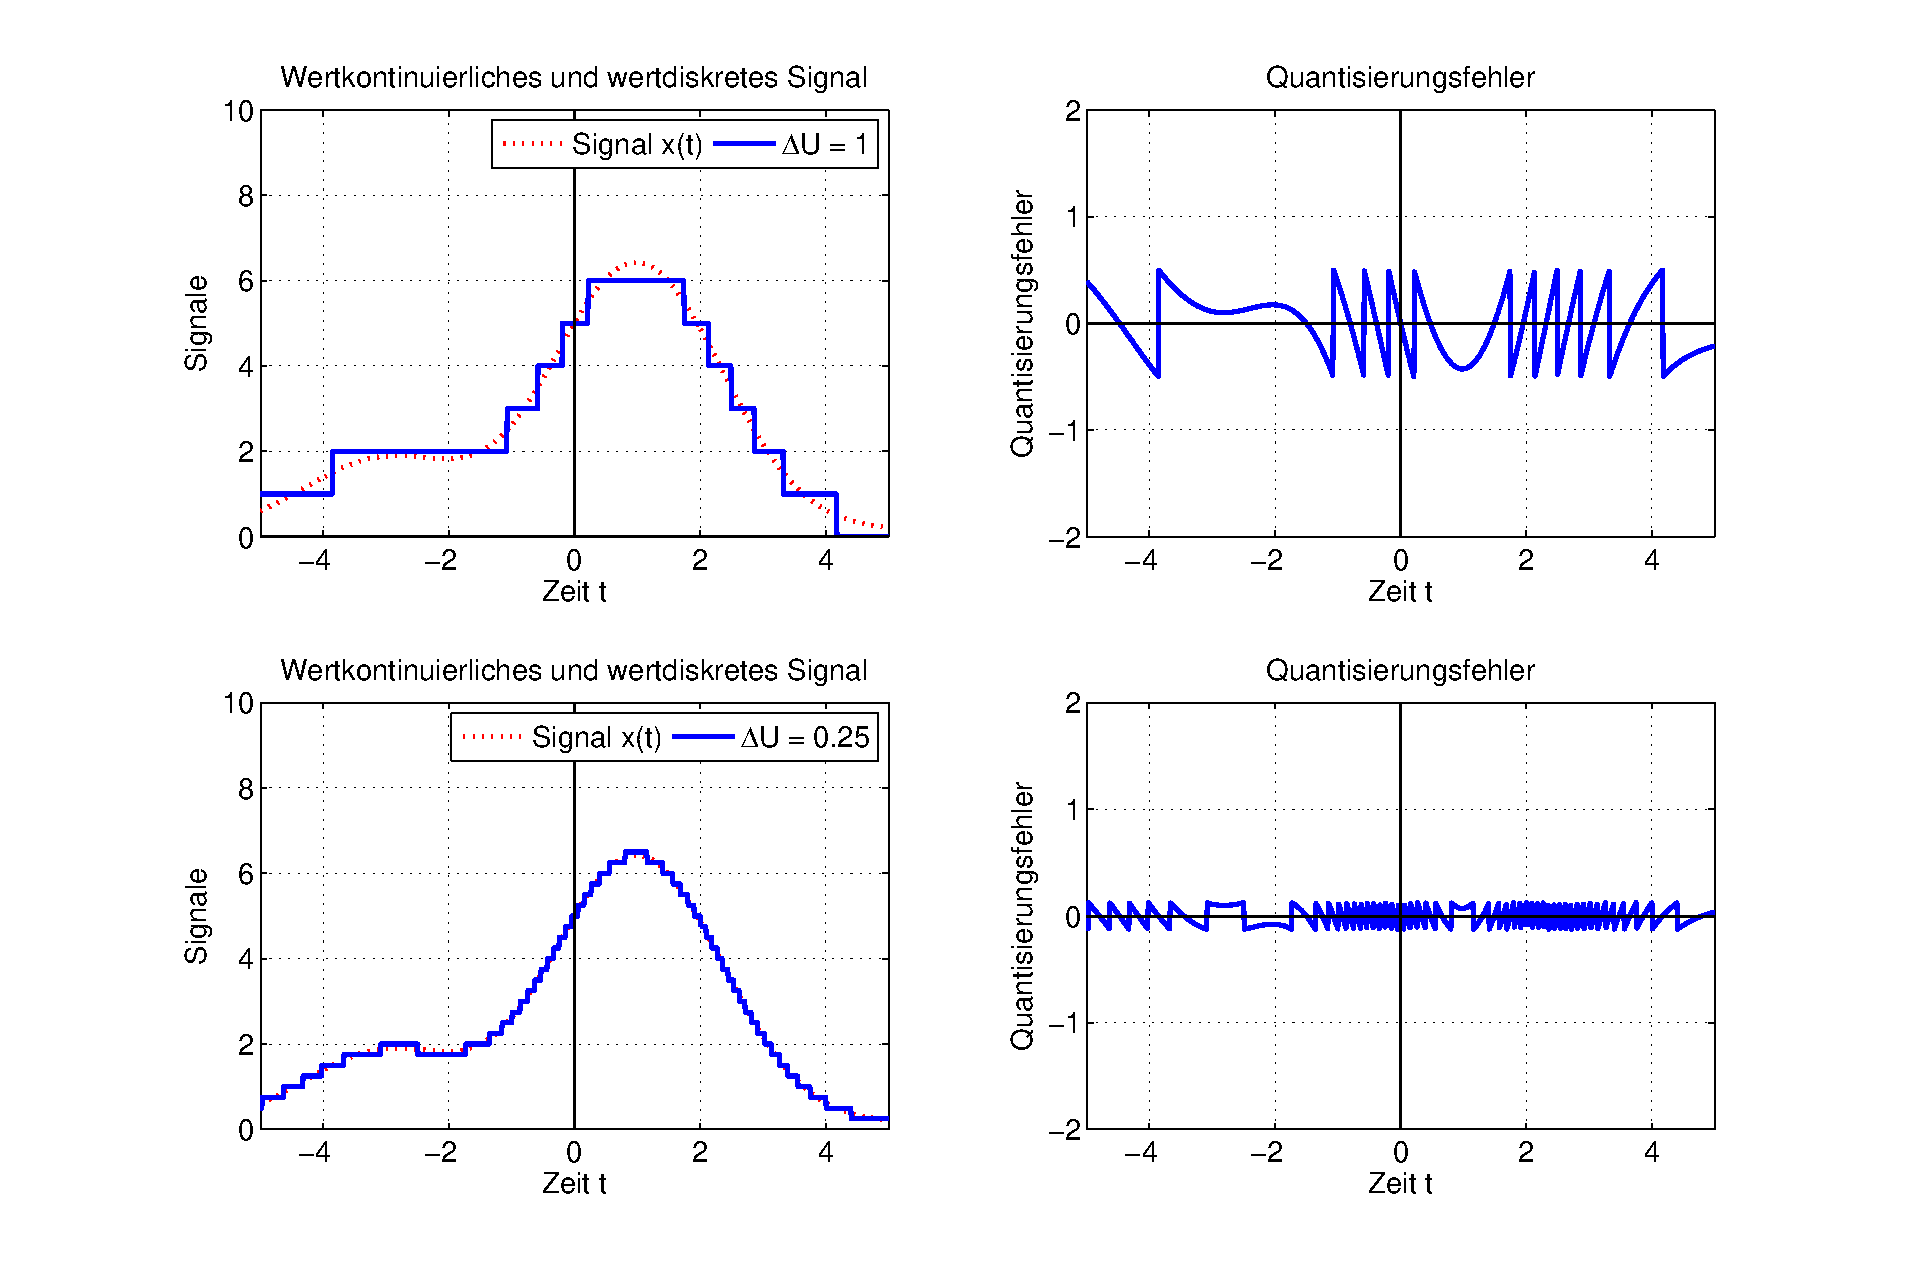
\includegraphics[width=1.0\textwidth]{Kapitel1/Bilder/image1.eps}
  \caption{Darstellung wertkontinuierlicher und wertdiskreter Signale in zeitkontinuierlicher und zeitdiskreter Form}
  \label{fig:DiskreKontinuerlich}
\end{figure}

\noindent In den folgenden Kapiteln beschränken sich die Darstellungen auf werte- und zeitkontinuierliche Signale. Der Übergang zu diskreten Signalen erfolgt mit dem Abtasttheorem im Teil B dieser Buchreihe.


\subsubsection{ Determinierte und zuf\"{a}llige Signale}
Determinierte Signale lassen sich durch eine mathematische Vorschrift in ihrem zeitlichen Verlauf angeben. Sie k\"{o}nnen implizit oder explizit definiert sein. Bei einem explizit definierten Signal l\"{a}sst sich der zu einem Zeitpunkt t geh\"{o}rende Wert direkt ablesen. Ein Beispiel daf\"{u}r ist eine abklingende Sinusfunktion.

\begin{equation}\label{eq:oneone}
x(t)=10\cdot e^{\displaystyle -a\cdot t^{2}} \cdot\sin (b\cdot t)
\end{equation}

\noindent Bei der impliziten Definition eines Signals ist der Signalwert zwar eindeutig bestimmt, er muss aber zun\"{a}chst durch weitere Umformungen bestimmt werden. Ein Beispiel f\"{u}r ein implizit definiertes Signal ist eine Differentialgleichung.

\begin{equation}\label{eq:onetwo}
\dfrac{dx}{dt} +3\cdot \dfrac{d^{2} x}{dt^{2} } =5\cdot x(t)+\sin (\omega \cdot t)
\end{equation}

\noindent mit der Anfangsbedingung y(t = 0) = y${}_{0}$. Unabh\"{a}ngig von der Art der Definition ist der Wert eines determinierten Signals zu jedem Zeitpunkt exakt definiert.

\noindent Zuf\"{a}llige Signale k\"{o}nnen nicht exakt angegeben werden, f\"{u}r sie sind lediglich statistische Eigenschaften bekannt. Beispiele f\"{u}r zuf\"{a}llige Signale sind Rauschsignale, Fernsehsignale oder Sprachsignale. Information, die \"{u}bertragen werden soll, ist zuf\"{a}llig. W\"{a}re das Signal bekannt, m\"{u}sste es nicht mehr \"{u}bertragen werden. Deshalb sind zuf\"{a}llige Signale in der Nachrichtentechnik von entscheidender Bedeutung. Bild \ref{fig:DeterminierteZuffaeligeSignale} zeigt jeweils ein Beispiel f\"{u}r ein determiniertes und ein zuf\"{a}lliges Signal.


\begin{figure}[H]
  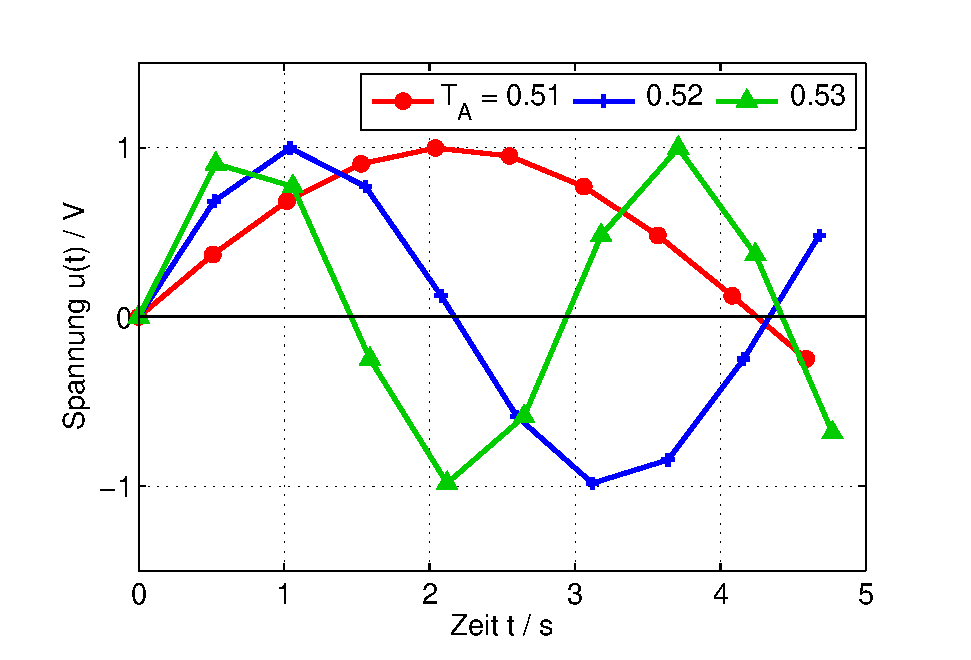
\includegraphics[width=1.0\textwidth]{Kapitel1/Bilder/image2.eps}
  \caption{Beispiele f\"{u}r determinierte und zuf\"{a}llige Signale}
  \label{fig:DeterminierteZuffaeligeSignale}
\end{figure}


\noindent In den Teilen A und B dieser Buchreihe werden determinierte Signale betrachtet. Zuf\"{a}llige Signale werden im Teil C dieser Buchreihe behandelt.


\subsubsection{ Zeitlich begrenzte und kausale Signale}
In der Systemtheorie wird oft mit zeitlich begrenzten Signalen gearbeitet. Ein Grund daf\"{u}r liegt in dem begrenzten Zeitraum, in dem ein System beobachtet werden kann. Ein weiterer Grund ist, dass f\"{u}r die Charakterisierung von Systemen teilweise Testsignale verwendet werden, die Spr\"{u}nge aufweisen. Auch diese Signale sind zumindest einseitig zeitbegrenzt. Bild \ref{fig:BegrenztKausal} zeigt zeitlich begrenzte Signale.


\begin{figure}[H]
  \centerline{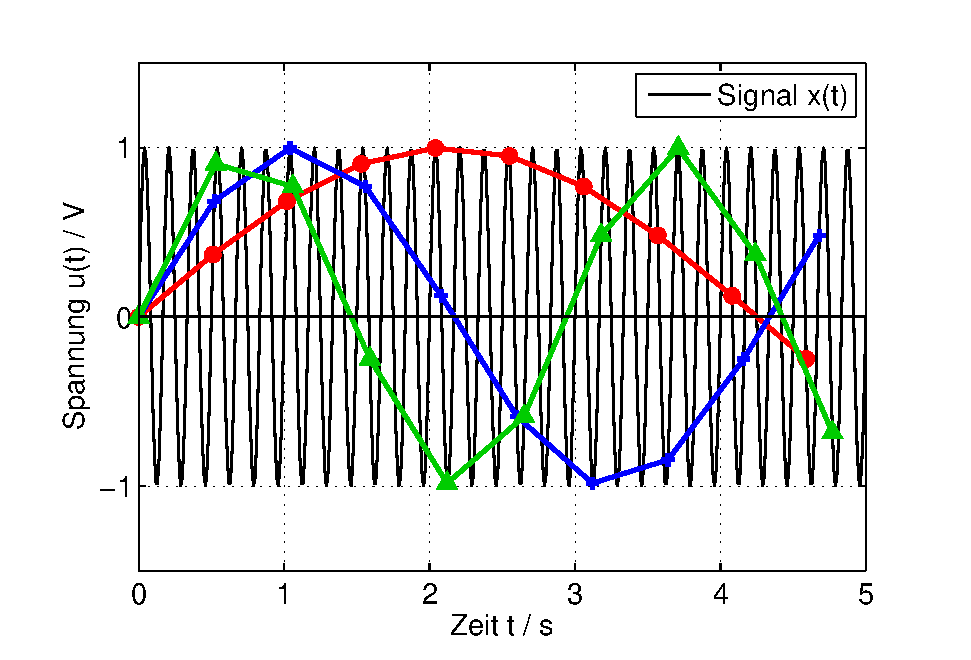
\includegraphics[width=1\textwidth]{Kapitel1/Bilder/image3.eps}}
  \caption{Darstellung eines beidseitig zeitbegrenzten und eines kausalen Signals}
  \label{fig:BegrenztKausal}
\end{figure}


\noindent Signale sind beidseitig zeitbegrenzt Signale, wenn sie nur f\"{u}r einen Zeitraum t${}_{1}$ $\leq$ t $\leq$ t${}_{2}$ von null verschieden sind. Einige Signale sind nur einseitig begrenzt, zum Beispiel ist ein zum Zeitpunkt t = t${}_{1}$ stattfindender Spannungssprung von 0 V auf 1 V nur einseitig zeitbegrenzt. Da diese Signale rechts auf dem Zeitstrahl von null verschieden sind, werden sie als rechtsseitige Signale bezeichnet. 

\noindent Ein kausales Signal ist ein spezielles rechtsseitiges Signal, für das gilt:

\begin{equation}\label{eq:onethree}
x\left(t\right)=0\quad \text{ für } t< 0 
\end{equation}

\noindent Auf die Bedeutung des Begriffes eines kausalen Signals wird bei der Diskussion von kausalen Systemen n\"{a}her eingegangen. 

\subsubsection{ Quadratisch integrierbare Signale}
F\"{u}r die Existenz von uneigentlichen Integralen zum Beispiel bei der Fourier-Transformation sind die Begriffe der Leistungs- und Energiesignale wesentlich. Zur Begriffsdefinition wird von der Vorstellung ausgegangen, dass die an einem Widerstand umgesetzte Leistung p${}_{EL}$(t) proportional zum Quadrat der anliegenden Spannung u(t) ist.


\begin{equation}\label{eq:onefour}
p_{EL} \left(t\right)=\dfrac{u^{2} \left(t\right)}{R} =i^{2} \left(t\right)\cdot R
\end{equation}

\noindent Die in dem Widerstand umgesetzte Energie ergibt sich aus dem Integral der umgesetzten Leistung \"{u}ber der Zeit.

\begin{equation}\label{eq:onefive}
E=\int\limits _{-\infty }^{\infty }p_{EL} \left(t\right) \; dt =\int\limits _{-\infty }^{\infty }\dfrac{u^{2} \left(t\right)}{R} \; dt =\int\limits _{-\infty }^{\infty }i^{2} \left(t\right)\cdot R\;dt 
\end{equation}

\noindent F\"{u}r den Vergleich von Systemen sind vielfach Leistungsverh\"{a}ltnisse von Bedeutung, sodass auf einen konstanten Faktor verzichtet wird. Verallgemeinernd wird die Energie eines Signals definiert als 

\begin{equation}\label{eq:onesix}
E=\int\limits _{-\infty }^{\infty }\left|x\left(t\right)\right|^{2} {\rm \; }dt
\end{equation}

\medskip

{\fontfamily{phv}\selectfont
\noindent\textbf{Energiesignale}} \smallskip

\noindent Energiesignale haben in dem Intervall von - $\infty$ $\mathrm{<}$ t $\mathrm{<}$ $\infty$ eine von Null verschiedene und endliche Gesamtenergie. Die mathematische Bedingung f\"{u}r Energiesignale lautet:

\begin{equation}\label{eq:oneseven}
0<\int\limits _{-\infty }^{\infty }\left|x\left(t\right)\right|^{2} \; dt<\infty
\end{equation}


\noindent Diese Bedingung ist f\"{u}r jedes zeitbegrenzte und amplitudenbegrenzte Signal erf\"{u}llt. Signale, die gleichzeitig zeit- und amplitudenbegrenzt sind, sind damit immer Energiesignale. Die Forderung nach gleichzeitiger Begrenzung von Zeitbereich und Amplitude ist hinreichend, aber nicht unbedingt notwendig.\\

\noindent
\colorbox{lightgray}{%
\arrayrulecolor{white}%
\renewcommand\arraystretch{0.6}%
\begin{tabular}{ wl{16.5cm} }
{\fontfamily{phv}\selectfont
\noindent{Beispiel: Energiesignal}} \smallskip
\end{tabular}%
}\bigskip

\noindent F\"{u}r das Signal x(t) mit  $a >  0$ soll gepr\"{u}ft werden, ob es sich um ein Energiesignal handelt.

\begin{equation}\label{eq:oneeight}
x(t)=e^{\displaystyle -\left|a\cdot t\right|}
\end{equation}

\noindent Das Signal x(t) ist f\"{u}r alle t mit  $-\infty < t < \infty$ definiert und ungleich null. Mit Gleichung \ref{eq:oneeight} errechnet sich die Energie des Signals zu

\begin{equation}\label{eq:onenine}
E=\int\limits _{-\infty }^{\infty }\left|e^{\displaystyle -\left|a\cdot t\right|} \right|^{2} \;  dt=2\cdot \int\limits _{0}^{\infty }e^{\displaystyle -2\cdot a\cdot t}  \;  dt=\left. 2\cdot \dfrac{e^{\displaystyle -2\cdot a\cdot t} }{-2\cdot a} \right|_{0}^{\infty } =2\cdot \dfrac{0-1}{-2\cdot a} =\dfrac{1}{a} 
\end{equation}


\noindent Die Energie des Signals ist endlich, das Signal x(t) ist demnach ein Energiesignal, das zeitlich nicht begrenzt ist. 

\noindent 

\noindent Bei vielen technischen Aufgabenstellungen weisen Signale eine endliche Energie auf, sodass diese Signale in der Systemtheorie von gro{\ss}er Bedeutung sind. Aus mathematischer Sicht handelt es sich bei den Energiesignalen um die Klasse der in dem Intervall von - $\infty$ $\mathrm{<}$ t $\mathrm{<}$ $\infty$ quadratisch integrierbaren Funktionen. \bigskip

{\fontfamily{phv}\selectfont
\noindent\textbf{Leistungssignale}} \smallskip

\noindent Leistungssignale haben im Intervall - $\infty$ $\mathrm{<}$ t $\mathrm{<}$ $\infty$ eine von Null verschiedene und endliche mittlere Leistung. Mathematisch ergibt sich folgende Definition f\"{u}r Leistungssignale:

\begin{equation}\label{eq:oneten}
\lim_{T \to \infty} \dfrac{1}{T}\cdot \int\limits _{-T/2}^{T/2}\left|x(t)\right|^{2} dt <\infty
\end{equation}

\noindent F\"{u}r Signale mit einer begrenzten Amplitude bedeutet das, dass sie nicht zeitbegrenzt sein m\"{u}ssen. Ihre Energie ist zwar unendlich, ihre Energie im Zeitintervall T ist aber begrenzt. 

\clearpage
\noindent
\colorbox{lightgray}{%
\arrayrulecolor{white}%
\renewcommand\arraystretch{0.6}%
\begin{tabular}{ wl{16.5cm} }
{\fontfamily{phv}\selectfont
\noindent{Beispiel: Leistungssignal }}
\end{tabular}%
}\bigskip

\noindent Ein Beispiel f\"{u}r ein Leistungssignal ist das konstante Signal x(t).

\begin{equation}\label{eq:oneeleven}
x\left(t\right)=c
\end{equation}

\noindent Einsetzen der Funktion in die Bedingung f\"{u}r Leistungssignale ergibt

\begin{equation}\label{eq:onetwelve}
\lim_{T \to \infty} \dfrac{1}{T}\cdot \int\limits _{-T/2}^{T/2}\left|x(t)\right|^{2} dt 
=\lim_{T \to \infty} \dfrac{1}{T}\cdot \int\limits _{-T/2}^{T/2}\left|c\right|^{2} dt 
=\lim_{T \to \infty} \dfrac{1}{T}\cdot T\cdot \left|c\right|^{2} =\left|c\right|^{2} <\infty
\end{equation}


\noindent Der Wert des Integrals ist endlich, sodass das Signal x(t) ein Leistungssignal ist. Die Energie des Signals ist unendlich, sodass das konstante Signal kein Energiesignal ist.

\begin{equation}\label{eq:onethirteen}
E=\int\limits _{-\infty }^{\infty }c^{2} \;  dt=c^{2} \cdot \int\limits _{-\infty }^{\infty }1 \;  dt=\infty
\end{equation}

\noindent Ein Vergleich der Definitionen von Leistungs- und Energiesignalen zeigt, dass ein Energiesignal stets ein Leistungssignal ist. Ist die Energie eines Signals endlich, gilt die Beziehung

\begin{equation}\label{eq:onefourteen}
\int\limits _{-\infty }^{\infty }\left|x\left(t\right)\right|^{2} \; dt=\lim_{T \to \infty}  \, \, \int\limits _{-T/2}^{T/2}\left|x\left(t\right)\right|^{2} \; dt<\infty
\end{equation}


\noindent Daraus folgt f\"{u}r die Leistung des Signals

\begin{equation}\label{eq:onefifteen}
\lim_{T \to \infty}  \, \, \dfrac{1}{T} \cdot \int\limits _{-T/2}^{T/2}\left|x(t)\right|^{2} \; dt=0
\end{equation}


\noindent Signale, die weder Energie- noch Leistungssignale sind, spielen in der Systemtheorie nur in Sonderf\"{a}llen eine Rolle, da die Systemtheorie technische Vorg\"{a}nge beschreibt, die grunds\"{a}tzlich mit einer endlichen Leistung verbunden sind.


\subsubsection{ Symmetrieeigenschaften zeitkontinuierlicher Signale}

\noindent Die Interpretation von Signalen vereinfacht sich, wenn ihre Symmetrieeigenschaften bekannt sind. Gerade und ungerade Signale weisen eine derartige Symmetrie auf. Gerade Signale sind f\"{u}r alle t symmetrisch zur Achse t = 0, also zur Ordinatenachse. F\"{u}r ein gerades Signal gilt deshalb die Bedingung: 

\begin{equation}\label{eq:onesixteen}
x(t)=x(-t)
\end{equation}


\noindent Ein kosinusf\"{o}rmiges Signal ist Beispiel f\"{u}r ein gerades Signal, denn es gilt:

\begin{equation}\label{eq:oneseventeen}
x_{1} \left(t\right)=\cos \left(\omega \cdot t\right)=\cos \left(-\omega \cdot t\right)=x_{1} \left(-t\right)
\end{equation}

\noindent Ungerade Signale sind f\"{u}r alle t punktsymmetrisch zu dem Koordinatenursprung. Diese Bedingung kann mathematisch ausgedr\"{u}ckt werden als

\begin{equation}\label{eq:oneeighteen}
x\left(t\right)=-x\left(-t\right)
\end{equation}

\noindent Ein sinusf\"{o}rmiges Signal ist ein Beispiel f\"{u}r ein ungerades Signal, denn es gilt:

\begin{equation}\label{eq:onenineteen}
x_{2} \left(t\right)=\sin \left(\omega \cdot t\right)=-\sin \left(-\omega \cdot t\right)=-x_{2} \left(-t\right)
\end{equation}


\noindent Bild \ref{fig:SymmetrieSinusKosinus} zeigt Kosinus- und Sinusfunktionen als Beispiele f\"{u}r gerade und ungerade Signale. Die Bedingung f\"{u}r gerade und ungerade Signale ist rot gestrichelt eingezeichnet.
\clearpage

\begin{figure}[H]
  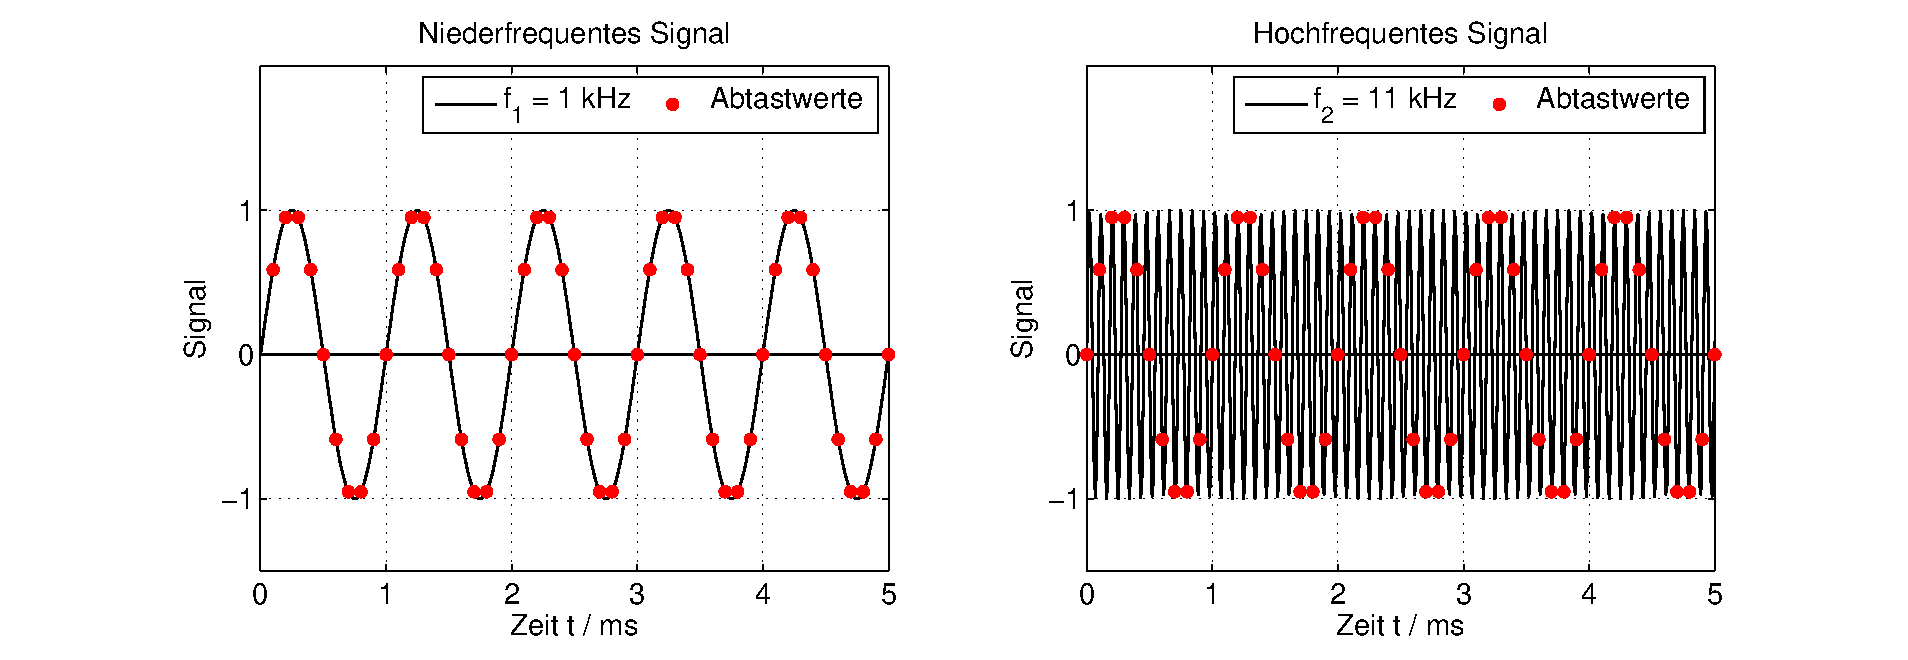
\includegraphics[width=1\textwidth]{Kapitel1/Bilder/image4}
  \caption{Kosinus- und Sinusfunktionen als Beispiele f\"{u}r gerade und ungerade Signale}
  \label{fig:SymmetrieSinusKosinus}
\end{figure}

\noindent Es existieren Signale, die weder gerade, noch ungerade sind, sie weisen keine Symmetrie auf. Jedes beliebige Signal l\"{a}sst sich aber in einen geraden Signalanteil x${}_{G}$(t) und einen ungeraden Signalanteil x${}_{U}$(t) aufspalten. 

\begin{equation}\label{eq:onetwenty}
x\left(t\right)=x_{G} \left(t\right)+x_{U} \left(t\right)
\end{equation}


\noindent wobei sich die beiden Anteile ergeben aus

\begin{equation}\label{eq:onetwentyone}
x_{G} \left(t\right)=\dfrac{1}{2} \cdot \left(x\left(t\right)+x\left(-t\right)\right)
\end{equation}


\noindent und 

\begin{equation}\label{eq:onetwentytwo}
x_{U} \left(t\right)=\dfrac{1}{2} \cdot \left(x\left(t\right)-x\left(-t\right)\right)
\end{equation}


\noindent Bild \ref{fig:GeradeUngerade} verdeutlicht die Zerlegung eines Signals in einen geraden und einen ungeraden Anteil an einem Beispiel.

\begin{figure}[H]
  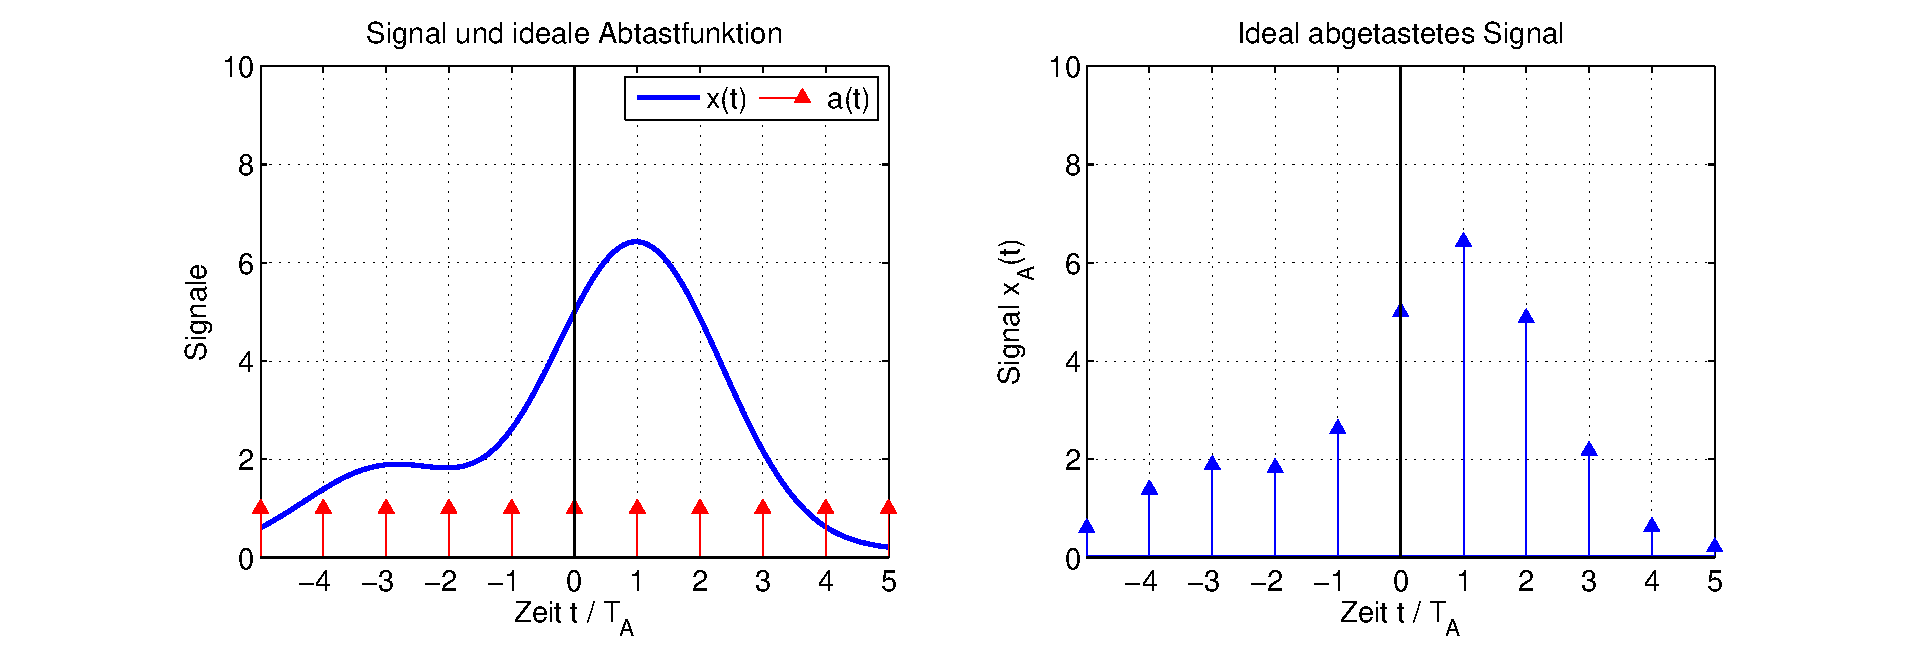
\includegraphics[width=1.0\textwidth]{Kapitel1/Bilder/image5}
  \caption{Zerlegung eines Signals in geraden und ungeraden Anteil}
  \label{fig:GeradeUngerade}
\end{figure}

\noindent Neben der Symmetrie reeller Signale wird zum Beispiel bei der Fourier-Transformation ein konjugiert symmetrisches Signal x*(t) verwendet. Ein Signal ist konjugiert symmetrisch, wenn die Beziehung 

\begin{equation}\label{eq:onetwentythree}
x(t)=x^{*} (-t)
\end{equation}

\noindent gilt.

\clearpage

\subsubsection{ Zusammenfassung Signaleigenschaften}

\noindent Zur besseren Übersicht sind in die Signaleigenschaften für zeit- und wertkontinuierliche Signale dargestellt. 


\begin{table}[H]
\setlength{\arrayrulewidth}{.1em}
\caption{Tabellarische Übersicht über Signaleigenschaften für zeit- und wertkontinuierliche Signale}

\setlength{\fboxsep}{0pt}%
\colorbox{lightgray}{%
\arrayrulecolor{white}%
\begin{tabular}{| l | l |}
\hline
\parbox[c][0.3in][c]{3in}{\smallskip\centering\textbf{\fontfamily{phv}\selectfont{Signaleigenschaft}}} & \parbox[c][0.3in][c]{3in}{\smallskip\centering\textbf{\fontfamily{phv}\selectfont{Mathematische Beschreibung}}}\\ \hline
\parbox[c][1in][c]{3in}{\smallskip\centering{\fontfamily{phv}\selectfont{Explizit definiertes Signal}}} & \parbox[c][1in][c]{3in}{\centering{\fontfamily{phv}\selectfont{Funktionswert kann direkt abgelesen werden,\\zum Beispiel\\[3pt]
$x(t)=10\cdot e^{\displaystyle -a\cdot t^{2}}\cdot\sin (b\cdot t)$}}}\\ \hline

\parbox[c][1in][c]{3in}{\centering{\fontfamily{phv}\selectfont{Implizit definiertes Signal}}} & \parbox[c][1in][c]{3in}{\centering{\fontfamily{phv}\selectfont{Funktionswert muss unter Ber\"{u}cksichtigung von Anfangsbedingungen berechnet werden, zum Beispiel\newline 
$\dfrac{dx}{dt} \; +3\cdot \dfrac{d^{2} x(t)}{dt^{2}} =5\cdot x(t)+\sin (\omega \cdot t)$}}}\\ \hline

\parbox[c][0.64in][c]{3in}{\centering{\fontfamily{phv}\selectfont{Begrenztes Signal}}} & \parbox[c][0.64in][c]{3in}{\centering{\fontfamily{phv}\selectfont{$x(t)=0$ \quad für $t<t_{1} $  und/oder  $ t>t_{2} $}}}\\ \hline

\parbox[c][0.64in][c]{3in}{\centering{\fontfamily{phv}\selectfont{Kausales Signal}}} & \parbox[c][0.64in][c]{3in}{\centering{\fontfamily{phv}\selectfont{$x(t)=0 $ für $t<0$}}}\\ \hline

\parbox[c][0.64in][c]{3in}{\centering{\fontfamily{phv}\selectfont{Energiesignal}}} & \parbox[c][0.64in][c]{3in}{\centering{\fontfamily{phv}\selectfont{$0<\int\limits _{-\infty }^{\infty }\left|x(t)\right|^{2} \; dt<\infty  $}}}\\ \hline

\parbox[c][0.64in][c]{3in}{\centering{\fontfamily{phv}\selectfont{Leistungssignal}}} & \parbox[c][0.64in][c]{3in}{\centering{\fontfamily{phv}\selectfont{$\lim\limits_{T\to \infty} \; \dfrac{1}{T} \cdot \int\limits _{-T/2}^{T/2}\left|x(t)\right|^{2} dt<\infty  $}}}\\ \hline

\parbox[c][0.64in][c]{3in}{\centering{\fontfamily{phv}\selectfont{Gerades Signal}}} & \parbox[c][0.64in][c]{3in}{\centering{\fontfamily{phv}\selectfont{$x(t)=x(-t)$}}}\\ \hline

\parbox[c][0.64in][c]{3in}{\centering{\fontfamily{phv}\selectfont{Ungerades Signal}}} & \parbox[c][0.64in][c]{3in}{\centering{\fontfamily{phv}\selectfont{$x(t)=-x(-t)$}}}\\ 
\hline

\parbox[c][0.64in][c]{3in}{\centering{\fontfamily{phv}\selectfont{Gerader Signalanteil}}} & \parbox[c][0.64in][c]{3in}{\centering{\fontfamily{phv}\selectfont{$x_{G} (t)=\dfrac{1}{2} \cdot (x(t)+x(-t))$}}}\\ 
\hline

\parbox[c][0.64in][c]{3in}{\centering{\fontfamily{phv}\selectfont{Ungerader Signalanteil}}} & \parbox[c][0.64in][c]{3in}{\centering{\fontfamily{phv}\selectfont{$x_{U} (t)=\dfrac{1}{2} \cdot \left(x(t)-x(-t)\right)$}}}\\ 
\hline

\parbox[c][0.64in][c]{3in}{\centering{\fontfamily{phv}\selectfont{Konjugiert symmetrisches Signal}}} & \parbox[c][0.64in][c]{3in}{\centering{\fontfamily{phv}\selectfont{$x(t)=x^{*} (-t)$}}}\\ 
\hline
\end{tabular}%
}
\label{tab:oneone}
\end{table}

\clearpage


\subsection{ Rechnen mit Sprung- und Impulsfunktion}


\subsubsection{ Allgemein}

\noindent Die Beschreibung und Interpretation von Systemen kann unter anderem \"{u}ber die Systemreaktion auf standardisierte Eingangssignale erfolgen. Deshalb werden in diesem Abschnitt Sprung- und Impulsfunktionen vorgestellt, weitere Funktionen daraus abgeleitet und das Rechnen mit Impulsfunktionen vertieft.


\subsubsection{ Sprungfunktion}

\noindent Die Sprungfunkton $\sigma$(t) ist als Grenzwert einer Funktion $\sigma$(t) definiert, die ihren Funktionswert in einem Zeitraum der Länge $\varepsilon$ von 0 auf 1 wechselt. Die Funktion $\sigma$(t) wird im Folgenden als verallgemeinerte Sprungfunktion $\sigma$(t) bezeichnet. Sie ist abschnittsweise definiert als 

\begin{equation}\label{eq:onetwentyfour}
\sigma _{\varepsilon} (t)=\left\{\begin{array}{ll}
{0 \qquad \quad \text{ für } t<-\varepsilon /2} \\
{\dfrac{1}{\varepsilon } \cdot  t +\dfrac{1}{2} \;\, \text{ für} -\varepsilon /2<t<\varepsilon /2} \\
{1 \qquad \quad \text{ für } \varepsilon /2 \le t} \end{array}\right.
\end{equation}


\noindent Ihr Funktionsverlauf ist Bild \ref{fig:NaeherungSprungfunktion} dargestellt.

\begin{figure}[H]
  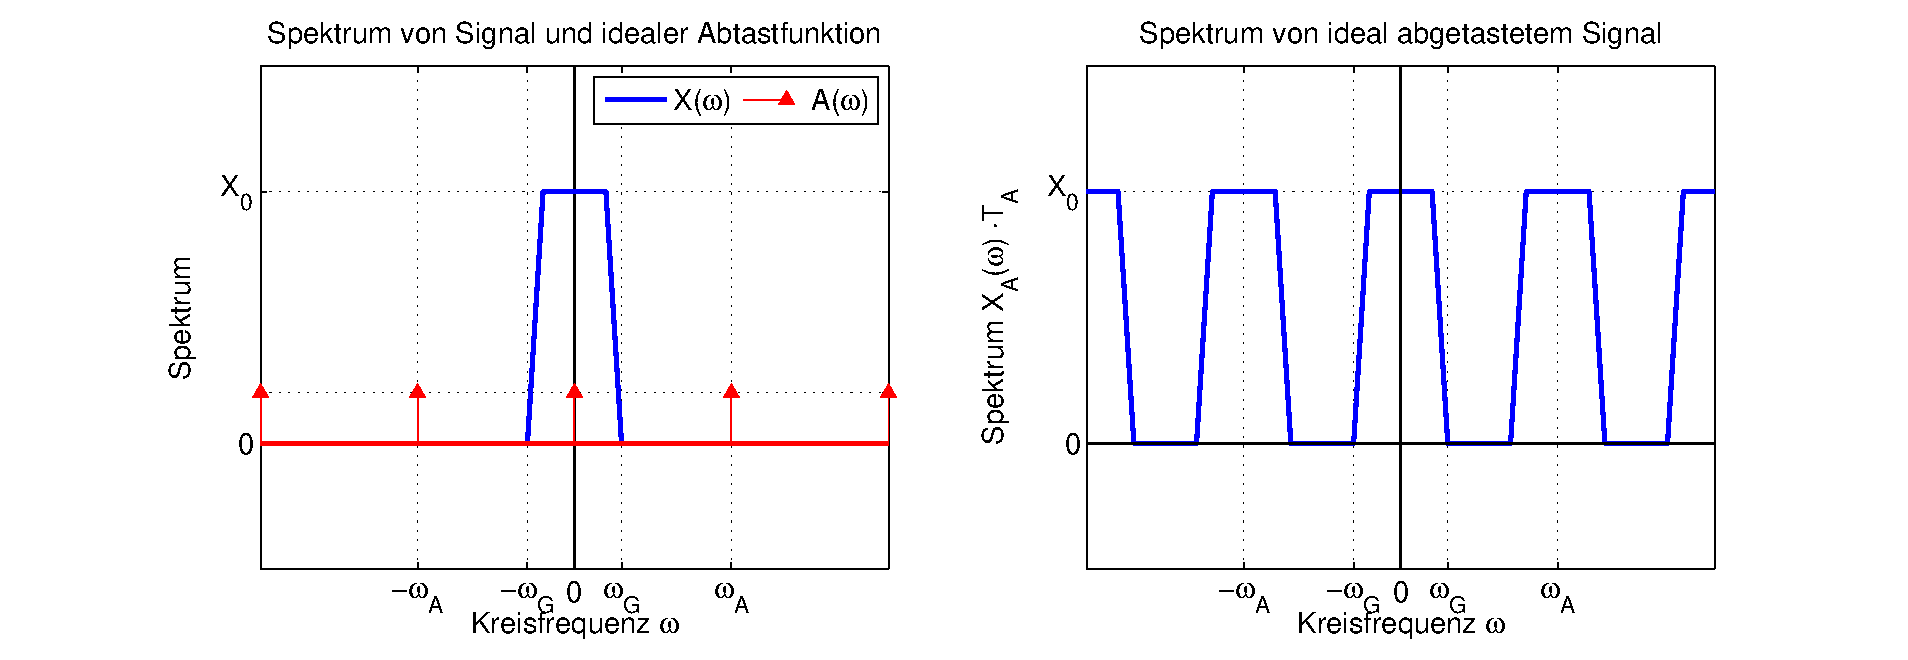
\includegraphics[width=1.0\textwidth]{Kapitel1/Bilder/image6.eps}
  \caption{Verallgemeinerte Sprungfunktion $\sigma$(t)}
  \label{fig:NaeherungSprungfunktion}
\end{figure}


\noindent Mit kleiner werdender Breite $\varepsilon$ wird der \"{U}bergang immer steiler. \"{U}ber eine Grenzwertbetrachtung $\epsilon$ $\rightarrow$ 0 geht die Funktion $\sigma$(t) in die Sprungfunktion $\sigma$(t) \"{u}ber, die an der Stelle t = 0 von 0 auf 1 springt. Die Sprungfunktion $\sigma$(t) ist abschnittsweise definiert als

\begin{equation}\label{eq:onetwentyfive}
x\left(t\right)=\sigma \left(t\right)=\left\{\begin{array}{l} 
{0\qquad \text{für } t<0} \\ 
{1\qquad \text{für } t \ge 0} 
\end{array}\right.\\
\end{equation}


\noindent F\"{u}r den Zeitpunkt t = 0 existieren in der Literatur unterschiedliche Definitionen. Im Hinblick auf diskrete Signale wird hier f\"{u}r den Zeitpunkt t = 0 der Funktionswert $\sigma$(t = 0) = 1 gew\"{a}hlt. 

\noindent Bei der Diskussion der Sprungstelle wird oftmals von rechtsseitigem und linksseitigem Grenzwert gesprochen. Der linksseitige Grenzwert wird als $\sigma$(0${}_{-}$) bezeichnet. Er hat den Wert der Funktion kurz vor dem Sprung $\sigma$(0${}_{-}$) = 0. Der rechtsseitige Grenzwert wird als $\sigma$(0${}_{+}$) bezeichnet. Er hat den Wert der Funktion kurz nach dem Sprung $\sigma$(0${}_{+}$) = 1. 

\noindent Die Sprungfunktion wird auch als Heaviside-Funktion bezeichnet. Sie wird zum Beispiel daf\"{u}r verwendet, Einschaltvorg\"{a}nge zu beschreiben. Die Sprungfunktion ist zeitlich nicht begrenzt, und sie ist kein Energiesignal. Wegen ihrer konstanten Amplitude ist die Bedingung f\"{u}r ein Leistungssignal erf\"{u}llt. Da die Sprungfunktion f\"{u}r t $\mathrm{<}$ 0 null ist, ist sie eine kausale Funktion.


\subsubsection{ Rechteckfunktion}

\noindent Die Rechteckfunktion ist abschnittsweise definiert als 

\begin{equation}\label{eq:onetwentysix}
x\left(t\right)=\left\{\begin{array}{l} 
{0\qquad \text{für }t<-T} \\ 
{1\qquad \text{für }-T{\le t<T}} \\ 
{0\qquad \text{für }T \le t} 
\end{array}\right.
\end{equation}


\noindent Die Rechteckfunktion ist eine Funktion mit endlicher Amplitude und endlicher Dauer. Die Bedingung f\"{u}r ein Energiesignal ist deshalb erf\"{u}llt. Die Funktion repr\"{a}sentiert damit ein Energie- und Leistungssignal. Sie ist nach Gleichung \ref{eq:onetwentysix} aber keine kausale Funktion, da sie f\"{u}r t $\mathrm{<}$ 0 nicht null ist. Durch eine Verschiebung um den Zeitraum T nach rechts kann die Rechteckfunktion in eine kausale Funktion \"{u}berf\"{u}hrt werden. Beide Funktionen sind in Bild \ref{fig:Rechteck} dargestellt.

\begin{figure}[ht]
  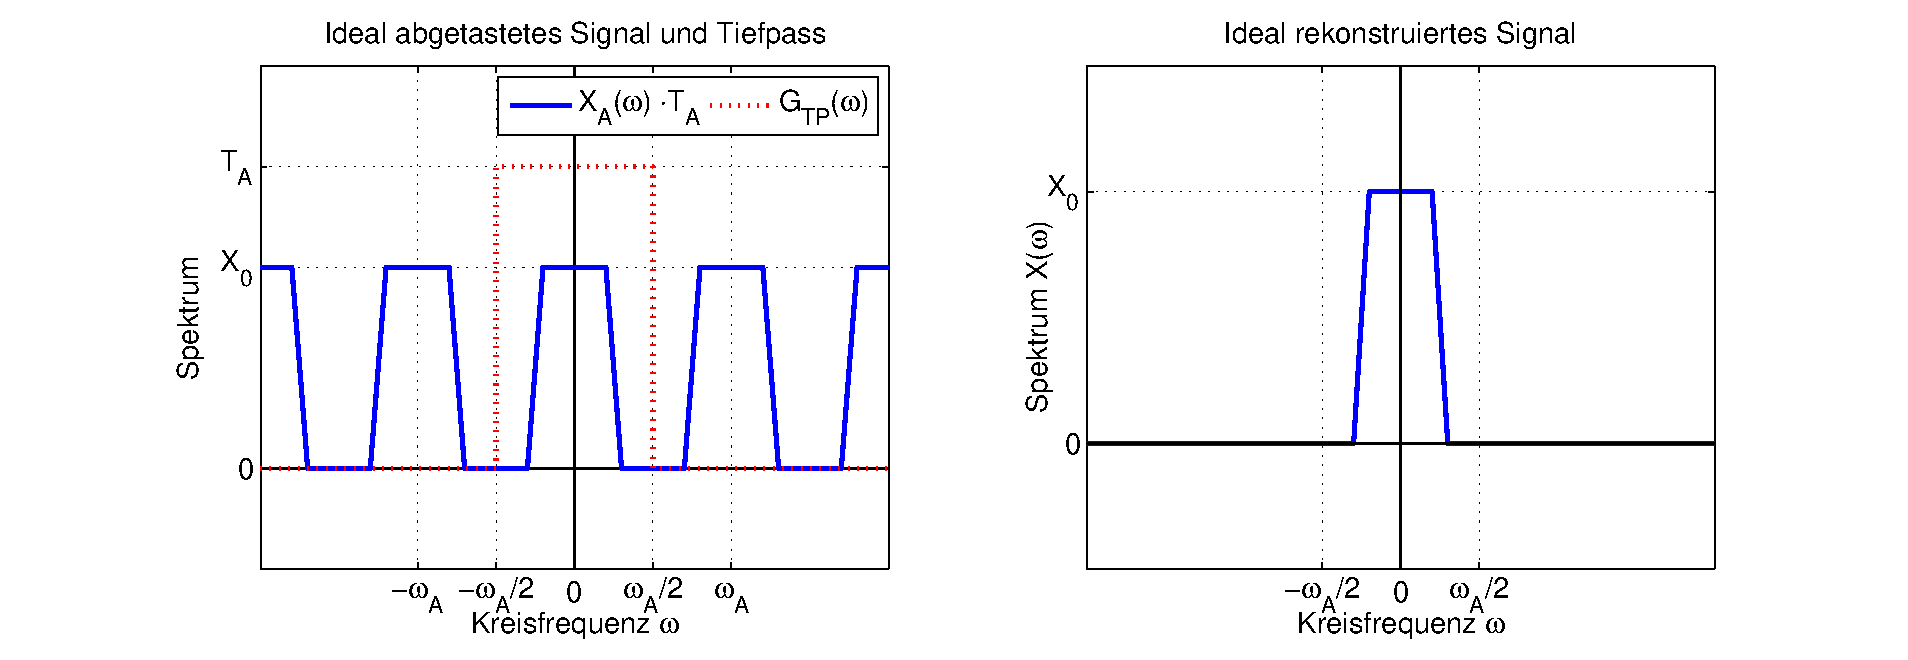
\includegraphics[width=1.0\textwidth]{Kapitel1/Bilder/image7}
  \caption{Rechteckfunktion und verschobene Rechteckfunktion}
  \label{fig:Rechteck}
\end{figure}


\noindent Die Rechteckfunktion kann neben der abschnittsweisen Definition auch als Summe zweier Sprungfunktionen dargestellt werden, die um - T beziehungsweise + T verschoben sind.

\begin{equation}\label{eq:onetwentyseven}
x_{1} \left(t\right)=\sigma \left(t+T\right)-\sigma \left(t-T\right)
\end{equation}


\noindent Entsprechend gilt f\"{u}r die kausale Rechteckfunktion

\begin{equation}\label{eq:onetwentyeight}
x_{2} \left(t\right)=\sigma \left(t\right)-\sigma \left(t-2\cdot T\right)
\end{equation}


\subsubsection{ Signum-Funktion }

\noindent Die Signum-Funktion sgn(t) ist abschnittsweise definiert als


\begin{equation}\label{eq:onetwentynine}
x(t)=sgn(t)=\left\{\begin{array}{l} {-{\rm 1\; }\quad \text{für } t<0} \\ 
{+1{\rm \; }\quad \text{für } 0 \le {\rm t\; }} \end{array}\right.
\end{equation}

\noindent Auch die Signum-Funktion kann mithilfe der Sprungfunktion dargestellt werden.

\begin{equation}\label{eq:onethirty}
x(t)=sgn(t)=2\cdot \sigma (t)-1
\end{equation}


\noindent Bild \ref{fig:Signum} stellt die Signum-Funktion grafisch dar. Sie ist unendlich lange ungleich null und ist kein Energiesignal. Wegen ihrer konstanten Amplitude ist die Bedingung f\"{u}r ein Leistungssignal erf\"{u}llt. Die Signum-Funktion ist nicht kausal und kann durch eine zeitliche Verschiebung auch nicht in ein kausales Signal \"{u}berf\"{u}hrt werden.


\begin{figure}[ht]
  \centerline{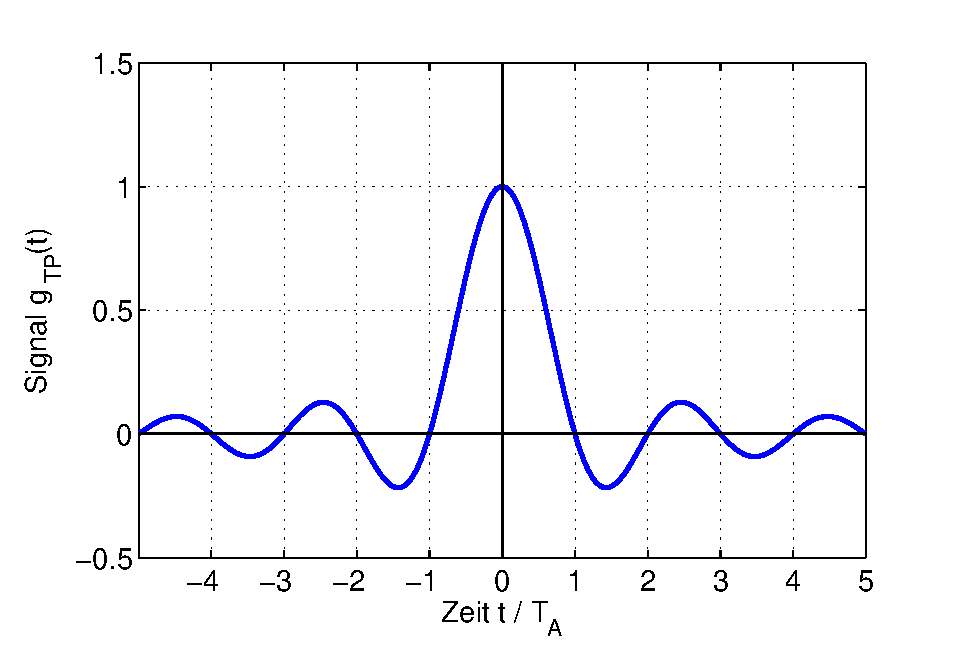
\includegraphics[width=0.5\textwidth]{Kapitel1/Bilder/image8.eps}}
  \caption{Signum-Funktion sgn(t)}
  \label{fig:Signum}
\end{figure}

\subsubsection{Rampenfunktion}

\noindent Ideale Sprung-, Rechteck- und Signum-Funktionen werden als Testsignale verwendet. Praktisch lassen sie sich wegen der unendlich gro{\ss}en Signal\"{a}nderung an den Unstetigkeitsstellen allerdings nur n\"{a}herungsweise realisieren. Au{\ss}erdem k\"{o}nnen Systeme, die mit einem sprungf\"{o}rmigen Signal angeregt werden, zerst\"{o}rt werden. Zum Beispiel werden die Schaufeln eines Turbinenrades, das sprungf\"{o}rmig mit einem gro{\ss}en Volumenstrom beaufschlagt wird, brechen. Die Rampenfunktion bietet einen stetigen \"{U}bergang der Funktionswerte f\"{u}r den Zeitraum t $\mathrm{<}$ 0 und den Zeitraum t $\mathrm{\ge}$ 0. Die Rampenfunktion ist definiert als

\begin{equation}\label{eq:onethirtyone}
x(t)=\left\{\begin{array}{ll} 
{0 \quad \text{ für }t<0} \\ 
{t \quad \text{ für }t \ge 0} 
\end{array}\right.
\end{equation}


\noindent Bild \ref{fig:Rampenfunktion} stellt die Rampenfunktion grafisch dar.

\begin{figure}[ht]
  \centerline{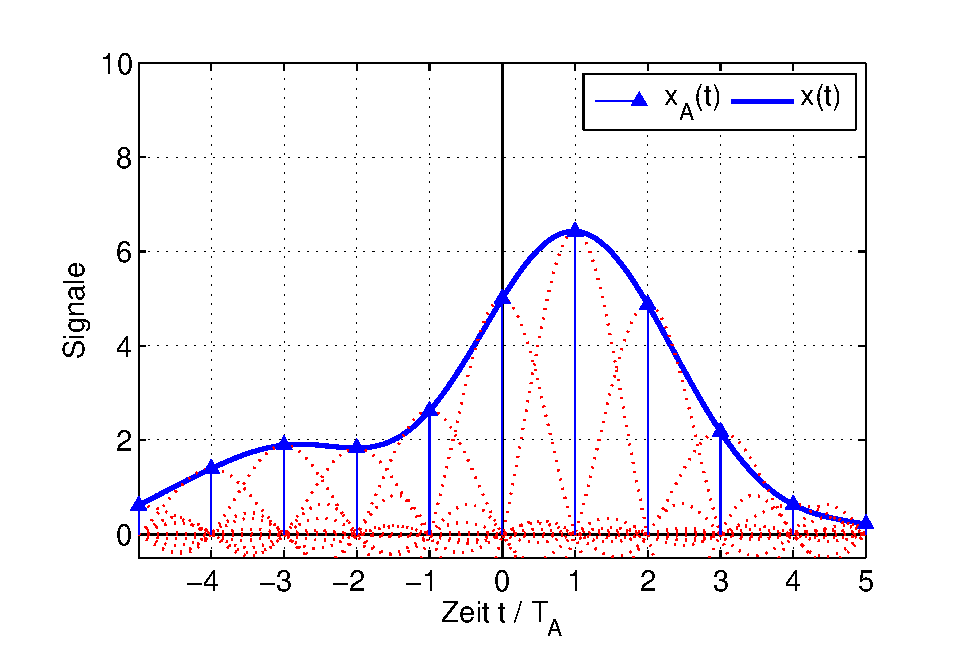
\includegraphics[width=0.5\textwidth]{Kapitel1/Bilder/image9}}
  \caption{Rampenfunktion}
  \label{fig:Rampenfunktion}
\end{figure}


\noindent Die Rampenfunktion kann sowohl als Integral der Sprungfunktion 

\begin{equation}\label{eq:onethirtytwo}
x\left(t\right)=\int\limits _{-\infty }^{t}\sigma \left(\tau \right) \;d\tau = \left\{\begin{array}{l} {0\qquad \text{für } t < 0} \\ 
{t\qquad \text{für } 0\le t} 
\end{array}\right.
\end{equation}


\noindent als auch als Produkt von Sprungfunktion und Zeit t dargestellt werden.

\begin{equation}\label{eq:onethirtythree}
x\left(t\right)=t\cdot \sigma \left(t\right)
\end{equation}


\noindent Die Rampenfunktion hat weder eine begrenzte Amplitude, noch eine begrenzte Zeitdauer, sie ist weder Energie- noch Leistungssignal. Eine ideale Rampenfunktion kann in realen Systemen deshalb nur f\"{u}r einen begrenzten Zeitraum realisiert werden. Da die Rampenfunktion f\"{u}r t $\mathrm{<}$ 0 null ist, beschreibt sie ein kausales Signal.


\subsubsection{ Dreieckfunktion}

\noindent Die Dreieckfunktion ist in Bild 1.10 dargestellt und definiert als

\begin{equation}\label{eq:onethirtyfour}
x\left(t\right)=\left\{\begin{array}{l} 
{0 \qquad \qquad \text{für } t<-T} \\ 
{1+t/T  \quad \,\: \text{ für } -T\le t<0} \\ 
{1-t/T  \quad \,\: \text{ für }  0\le t<T} \\ 
{0 \qquad \qquad \text{für } T\le t} 
\end{array}\right.
\end{equation}


\noindent Bild \ref{fig:DreieckFunktion} stellt eine Dreieckfunktion und eine verschobene Dreieckfunktion grafisch dar.

\begin{figure}[ht]
  \centerline{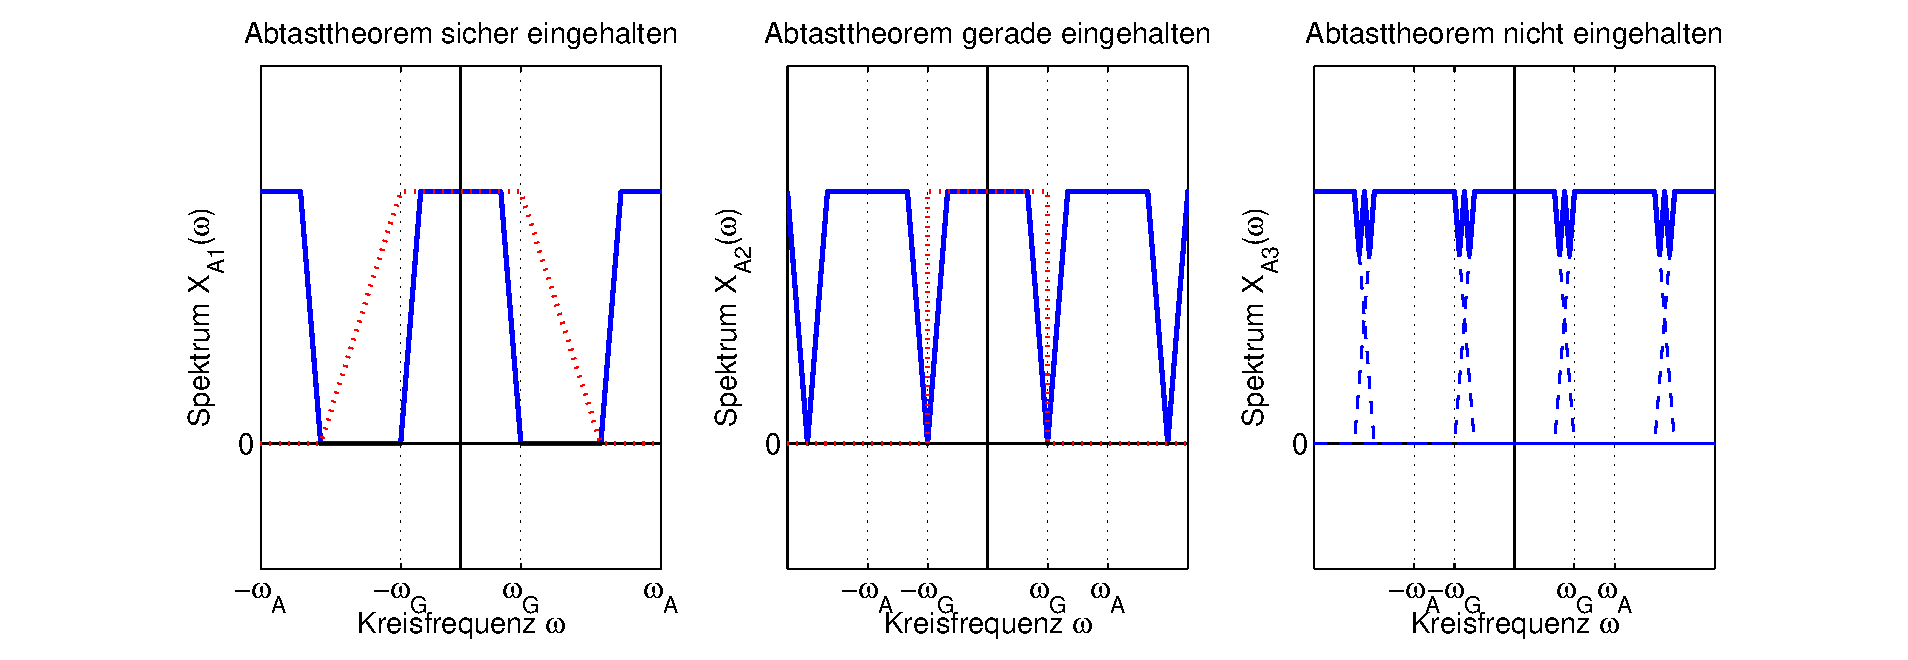
\includegraphics[width=0.9\textwidth]{Kapitel1/Bilder/image10.eps}}
  \caption{Dreieckfunktion und verschobene Dreieckfunktion}
  \label{fig:DreieckFunktion}
\end{figure}

\noindent Die Dreieckfunktion ist eine Funktion mit endlicher Amplitude und endlicher Dauer. Die Bedingung f\"{u}r ein Energiesignal ist erf\"{u}llt. Die Dreieckfunktion ist damit ein Energie- und Leistungssignal. Wie die Rechteckfunktion beginnt die Dreieckfunktion bereits f\"{u}r t = - T. Sie ist deshalb nicht kausal, kann aber durch Verschiebung um den Zeitraum T nach rechts in ein kausales Signal \"{u}berf\"{u}hrt werden.

\noindent Die Dreieckfunktion kann auf unterschiedliche Art aus den bereits dargestellten Funktionen gewonnen werden, zum Beispiel durch \"{U}berlagerung von drei Rampenfunktionen. 

\clearpage

\subsubsection{ Impulsfunktion}

\noindent Von gro{\ss}er Bedeutung f\"{u}r die theoretische Charakterisierung von Systemen ist die Impulsfunktion $\delta$(t). Die Impulsfunktion ist als Grenzwert einer Rechteckfunktion $\delta$(t) definiert, die eine Breite $\epsilon$ und der H\"{o}he 1/$\epsilon$ aufweist. Bild \ref{fig:NaehrungImpulsfunktion} zeigt den Rechteckimpuls.


\begin{equation}\label{eq:onethirtyfive}
\delta _{\varepsilon }(t)=\dfrac{1}{\varepsilon } \cdot \left(\sigma \left(t+\dfrac{\varepsilon }{2} \right)-\sigma \left(t-\dfrac{\varepsilon }{2} \right)\right)
\end{equation}

\begin{figure}[ht]
  \centerline{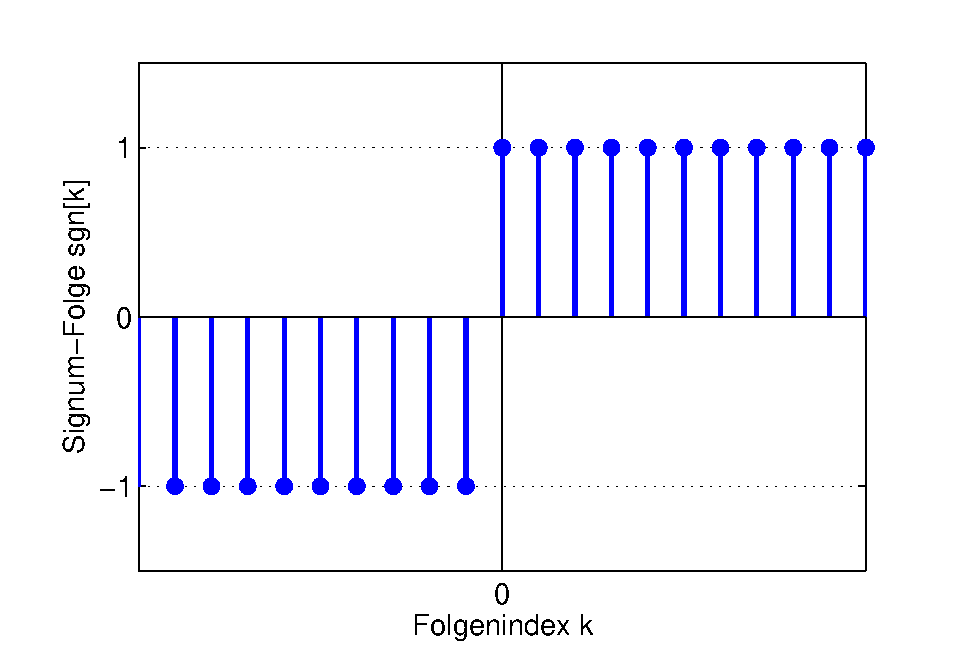
\includegraphics[width=0.5\textwidth]{Kapitel1/Bilder/image11}}
  \caption{Rechteckfunktion mit endlicher Breite $\varepsilon$ zur Ann\"{a}herung der Impulsfunktion}
  \label{fig:NaehrungImpulsfunktion}
\end{figure}

\noindent Mit kleiner werdender Breite $\varepsilon$ wird der das Rechteck immer schmaler, aber auch h\"{o}her, so dass die Fl\"{a}che des Rechtecks immer gleich 1 bleibt. \"{U}ber eine Grenzwertbetrachtung $\varepsilon$ $\rightarrow$ 0 geht diese Rechteckfunktion $\delta$(t) in die Impulsfunktion $\delta$(t) \"{u}ber.

\begin{equation}\label{eq:onethirtysix}
\delta (t)={\lim\limits_{\displaystyle \varepsilon \to 0}} {\rm \; }\left\{\begin{array}{l} 
{0 \qquad \text{ für } \; t<-\varepsilon /2} \\
{1/\varepsilon \quad \, \text{ für } - \varepsilon {\rm /2}<t<\varepsilon /2} \\ 
{0\qquad \text{ für } \; \varepsilon /2{\rm \; }\le {\rm t}} \end{array}\right.
\end{equation}


\noindent Bei der Impulsfunktion $\delta$(t) handelt sich um einen unendlich kurzen Impuls an der Stelle t = 0, der eine unendlich gro{\ss}e H\"{o}he hat. Die Gr\"{o}{\ss}e wird durch einen Pfeil der L\"{a}nge 1 an der Stelle t = 0 dargestellt, weil die Fl\"{a}che unter der Impulsfunktion den Fl\"{a}cheninhalt 1 aufweist. 

\begin{figure}[ht]
  \centerline{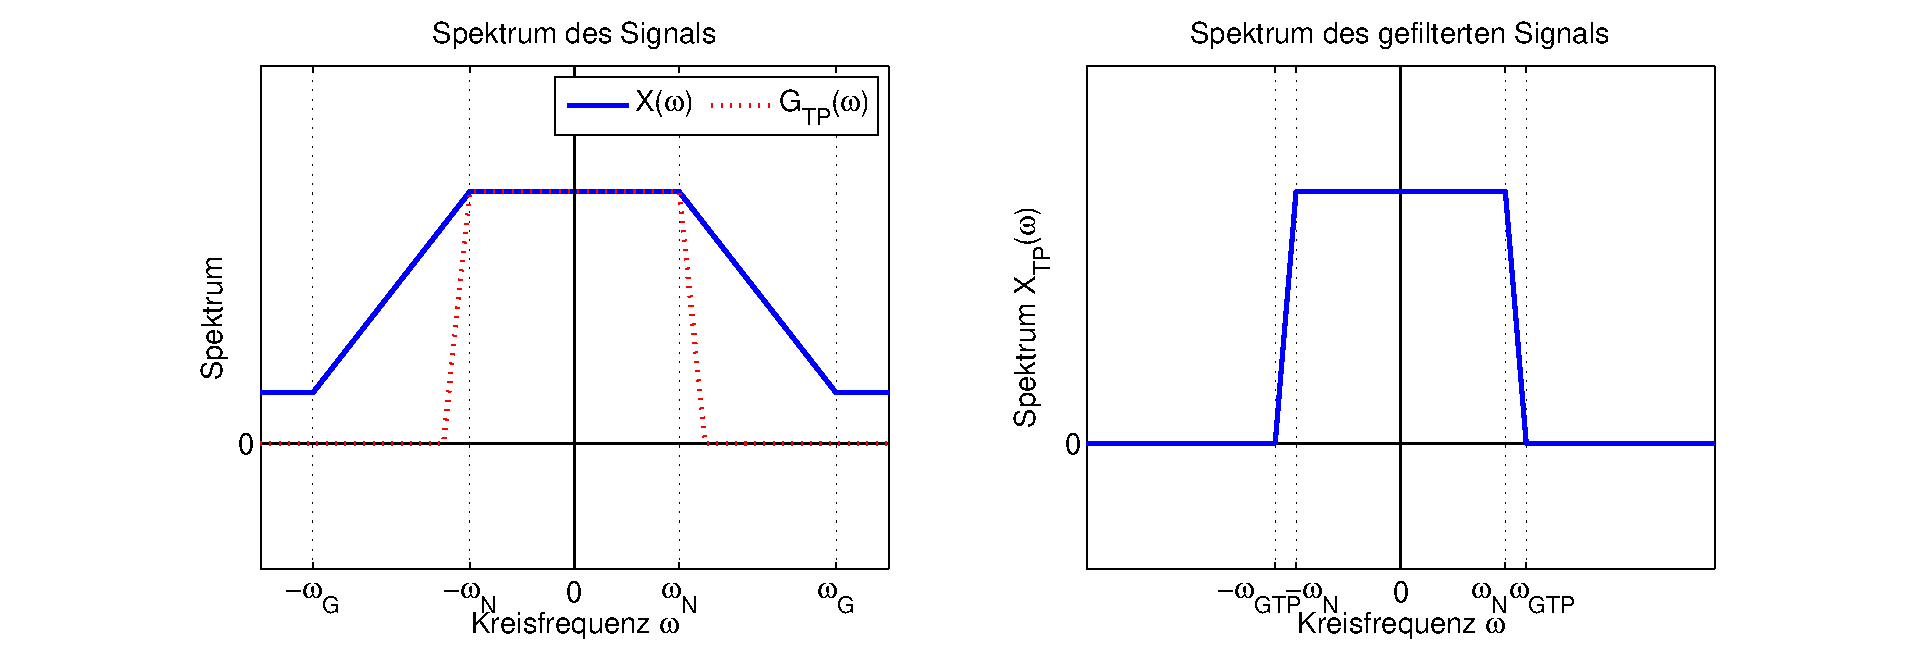
\includegraphics[width=0.5\textwidth]{Kapitel1/Bilder/image12}}
  \caption{Impulsfunktion $\delta$(t)}
  \label{fig:Impulsfunktion}
\end{figure}

\clearpage

\noindent Die Impulsfunktion ist eine gerade Funktion, denn es gilt die Beziehung 

\begin{equation}\label{eq:onethirtyseven}
\delta \left(t\right)=\delta \left(-t\right).
\end{equation}


\noindent Die Impulsfunktion ist eine kausale Funktion, da sie f\"{u}r t $\mathrm{<}$ 0 den Wert null besitzt, und sie ist ein Energiesignal, da sie eine begrenzte Energie besitzt.

\noindent Die Impulsfunktion wird aus Dirac-Impuls bezeichnet und ist als Grenzwert einer gew\"{o}hnlichen Funktion beschrieben. Neben der dargestellten Herleitung \"{u}ber die Rechteckfunktion wird in einem Projekt am Ende dieses Kapitels die Gau{\ss}funktion zur N\"{a}herung des Impulses verwendet. In dem Projekt wird der Impuls anschaulich verglichen mit einem Hammerschlag auf ein schwingungsf\"{a}higes System, zum Beispiel einer Glocke. Das System wird f\"{u}r eine extrem kurze Zeit mit gro{\ss}er Leistung angeregt. Die Glocke antwortet auf die Anregung mit einer Schwingung, die charakteristisch f\"{u}r sie ist. Es wird sich zeigen, dass bestimmte Systeme durch ihre Antwort auf einen Impuls am Eingang vollst\"{a}ndig charakterisiert sind.


\subsubsection{ Rechnen mit Impulsfunktionen}

\noindent Die Impulsfunktion ist Gegenstand der Distributionstheorie [Gelf60]. Hier soll auf Basis der vorgestellten Grenzwertbetrachtung eine anwendungsorientierte Anschauung vermittelt werden, die nicht weiter auf die Distributionstheorie eingeht. Die Gleichung \ref{eq:onethirtyfive} beschreibt den Impuls \"{u}ber eine Rechteckfunktion.

\begin{equation}\label{eq:onethirtyeight}
\delta _{\varepsilon } \left(t\right)=\dfrac{1}{\varepsilon } \cdot \left(\sigma \left(t+\dfrac{\varepsilon }{2} \right)-\sigma \left(t-\dfrac{\varepsilon }{2} \right)\right) \\
\end{equation}
\bigskip

{\fontfamily{phv}\selectfont
\noindent\textbf{Integral der Impulsfunktion}} \smallskip

\noindent Das Integral der Funktion von t = - $\infty$ bis + $\infty$ berechnet sich zu

\begin{equation}\label{eq:onethirtynine}
\int\limits _{-\infty }^{\infty }\delta \left(t\right) \; dt ={\mathop{\lim }\limits_{\varepsilon \to 0}} \; \int\limits _{-\varepsilon /2}^{\varepsilon /2}1/\varepsilon \; dt ={\mathop{\lim }\limits_{\varepsilon \to 0}} \; \dfrac{1}{\varepsilon } \cdot \left(\dfrac{\varepsilon }{2} -\left(-\dfrac{\varepsilon }{2} \right)\right)=\left(\dfrac{\varepsilon }{2\cdot \varepsilon } -\left(-\dfrac{\varepsilon }{2\cdot \varepsilon } \right)\right)=1
\end{equation}


\noindent Das Integral über die Impulsfunktion ist demnach 1. Das Integral der Impulsfunktion wird als Gewicht der Impulsfunktion bezeichnet und wie in Bild \ref{fig:Impulsfunktion} mit einem Pfeil der Länge 1 dargestellt. \bigskip

{\fontfamily{phv}\selectfont
\noindent\textbf{Stammfunktion der Impulsfunktion}} \smallskip

\noindent Die Stammfunktion der Impulsfunktion wird \"{u}ber die N\"{a}herung f\"{u}r die Impulsfunktion bestimmt. Sie ergibt sich mit der Rechteckfunktion $\delta$(t) aus

\begin{equation}\label{eq:onefourty}
\int\limits _{-\infty }^{t}\delta _{\varepsilon } \left(\tau \right) \; d\tau  =\left\{\begin{array}{ll}
{0\qquad \qquad \text{ für } t<-\varepsilon /2} \\
{\dfrac{1}{\varepsilon } \cdot t+\dfrac{ 1}{ 2} \quad \text{ für } -\varepsilon /2<t<\varepsilon /2} \\ 
{1\qquad \qquad  \text{ für }\varepsilon /2 \le t} \end{array}\right. \\
\end{equation}

\noindent Diese Funktion ist die in Bild 2.6 dargestellte verallgemeinerte Sprungfunktion $\sigma$(t). F\"{u}r die hier vorgestellte Grenzwertbetrachtung ergibt sich f\"{u}r die Ableitung der verallgemeinerten Sprungfunktion $\sigma$(t)

\begin{equation}\label{eq:onefourtyone}
\dfrac{d\sigma _{\varepsilon } }{dt} =\left. \left\{\begin{array}{l} 
{0 \qquad \; \text{ für } t<-\varepsilon /2} \\
{\dfrac{1}{\varepsilon} \qquad \text{ für } - \varepsilon /2 <t< \varepsilon /2} \\ 
{0 \qquad \; \text{ für } \varepsilon /2 \le t} \end{array}\right. \right\}=\delta _{\varepsilon } \left(t\right)\\
\end{equation}


\noindent F\"{u}r den Grenzwert $\varepsilon$ $\rightarrow$ 0 ergibt sich die Ableitung der Sprungfunktion

\begin{equation}\label{eq:onefourtytwo}
\dfrac{d\sigma }{dt} =\delta \left(t\right)
\end{equation}


\noindent und umgekehrt die Stammfunktion der Impulsfunktion

\begin{equation}\label{eq:onefourtythree}
\int\limits _{-\infty }^{t}\delta \left(\tau \right){\rm \; }d\tau  =\sigma \left(t\right)
\end{equation}

\bigskip

{\fontfamily{phv}\selectfont
\noindent\textbf{Ausblendeigenschaft der Impulsfunktion}} \smallskip

\noindent Aus der Auswertung des folgenden Integrals ergibt sich eine weitere wichtige Eigenschaft der Impulsfunktion, n\"{a}mlich die Ausblendeigenschaft der Impulsfunktion. Ausgangspunkt ist die Gleichung 

\begin{equation}\label{eq:onefourtyfour}
\int\limits _{-\infty }^{\infty }\delta (t)\cdot x(t) \: dt ={\lim \limits_{\displaystyle\varepsilon \to 0}} \; \dfrac{1}{\varepsilon } \cdot \int\limits _{-\varepsilon /2}^{\varepsilon /2}x(t) \: dt
\end{equation}

\noindent Nach dem Mittelwertsatz der Integralrechnung gibt es ein $t_{0}$ mit $a < t_{0} < b$, f\"{u}r das gilt:

\begin{equation}\label{eq:onefourtyfive}
\int\limits _{a}^{b}x(t) \; dt =(b-a)\cdot x(t_{0} )
\end{equation}

\noindent Damit ergibt sich f\"{u}r Gleichung \ref{eq:onefourtyfour}

\begin{equation}\label{eq:onefourtysix}
\int\limits _{-\infty }^{\infty }\delta (t)\cdot x(t) \; dt ={\lim \limits_{\varepsilon \to 0}} {\rm \; }\dfrac{1}{\varepsilon } \cdot \int\limits _{-\varepsilon /2}^{\varepsilon /2}x(t) \; dt =x(0)
\end{equation}

\noindent Mit dieser Rechenvorschrift l\"{a}sst sich der Abtastwert der Funktion x(t) zum Zeitpunkt t = 0 beschreiben. Die Methode kann f\"{u}r beliebige Zeitpunkte t${}_{0}$ verallgemeinert werden zu

\begin{equation}\label{eq:onefourtyseven}
\int\limits _{-\infty }^{\infty }\delta \left(t-t_{0} \right)\cdot x\left(t\right)\;dt =\int\limits _{-\infty }^{\infty }\delta \left(t\right)\cdot x\left(t+t_{0} \right)\;dt =x\left(t_{0} \right)
\end{equation}

\noindent Die Ausblendeigenschaft der Impulsfunktion wird in Bild \ref{fig:twoAusblendeigenschaftImpulsfunktion} grafisch veranschaulicht. 

\begin{figure}[H]
  \centerline{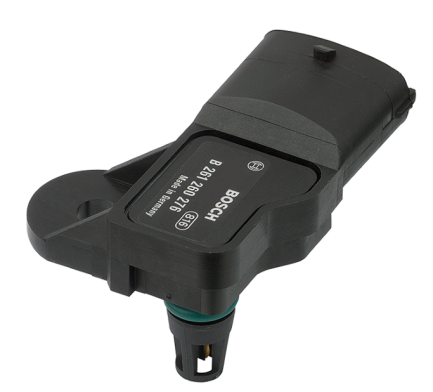
\includegraphics[width=1\textwidth]{Kapitel1/Bilder/image13}}
  \caption{Grafische Darstellung der Ausblendeigenschaft}
  \label{fig:twoAusblendeigenschaftImpulsfunktion}
\end{figure}

\noindent 

\noindent Die Funktion x(t) und die Impulsfunktion an der Stelle t${}_{0}$ sind im Bild links dargestellt. Beide Funktionen werden miteinander multipliziert, das Produkt besteht aus einem Impuls an der Stelle t${}_{0}$ mit dem Gewicht x(t${}_{0}$). Er wird im rechten Bildteil gezeigt. Da das Gewicht des Impulses eine Konstante ist, kann sie aus dem Integral gezogen werden. \"{U}brig bleibt das Integral \"{u}ber eine Impulsfunktion, das nach den diskutierten Rechenregeln den Wert eins aufweist.
\bigskip

{\fontfamily{phv}\selectfont
\noindent\textbf{Ableitung der Impulsfunktion}} \smallskip

\noindent Die Ableitung der Impulsfunktion ist nur bei der Auswertung von Integralen von Bedeutung. In diesem Fall kann die Ableitung durch Anwendung der partiellen Integration umgangen werden.

\begin{equation}\label{eq:onefourtyeight}
\int\limits _{-\infty }^{\infty }\dfrac{d\delta }{dt} \cdot x(t) dt = \delta (t) \cdot x(t)|_{-\infty }^{\infty } -\int\limits _{-\infty }^{\infty }\delta (t)\cdot \dfrac{dx}{dt} dt =-\int\limits _{-\infty }^{\infty }\delta (t)\cdot \dfrac{dx}{dt} dt = -\left. \dfrac{dx}{dt} \right|_{t=0}
\end{equation}

\bigskip

{\fontfamily{phv}\selectfont
\noindent\textbf{Zeitliche Skalierung}} \smallskip

\noindent Wird die Impulsfunktion skaliert, ergibt sich die Funktion

\begin{equation}\label{eq:onefourtynine}
x(t)=\delta (a\cdot t)
\end{equation}


\noindent Mit a $\mathrm{>}$ 0 errechnet sich das Integral in Gleichung \ref{eq:onefourtynine} nach Substitution zu

\begin{equation}\label{eq:fifty}
\int\limits _{-\infty }^{\infty }\delta (a\cdot t) \: dt =\dfrac{1}{a} \cdot \int\limits _{-\infty }^{\infty }\delta (a\cdot t) \: d(a\cdot t) =\dfrac{1}{a}
\end{equation}


\noindent 

\noindent F\"{u}r negative Werte a muss zus\"{a}tzlich die Integrationsreihenfolge ge\"{a}ndert werden, und es ergibt sich ein negatives Vorzeichen. Allgemein gilt 

\begin{equation}\label{eq:onefiftyone}
\int\limits _{-\infty }^{\infty }\delta (a\cdot t) dt =\dfrac{1}{|a|}
\end{equation}


\noindent Eine mit a skalierte Impulsfunktion weist demnach das Gewicht 1/{\textbar}a{\textbar} auf.

\clearpage

\subsubsection{ Zusammenfassung Testfunktionen}

\noindent In Tabelle \ref{tab:twotwo} sind die wesentlichen Testfunktionen und in Tabelle \ref{tab:twothree} die Eigenschaften der Impulsfunktion zusammengefasst.\\


\begin{table}[H]
\setlength{\arrayrulewidth}{.1em}
\caption{Tabellarische Zusammenfassung von Testfunktionen}
\setlength{\fboxsep}{0pt}%
\colorbox{lightgray}{%
\arrayrulecolor{white}%
\begin{tabular}{| l | l |}
\hline
\parbox[c][0.28in][c]{3.3in}{\smallskip\centering\textbf{\fontfamily{phv}\selectfont{Testfunktion}}} & \parbox[c][0.28in][c]{3.3in}{\smallskip\centering\textbf{\fontfamily{phv}\selectfont{Mathematische Beschreibung}}}\\ \hline

\parbox[c][0.64in][c]{3.3in}{\centering{\fontfamily{phv}\selectfont{Sprungfunktion}}} & 
\parbox[c][0.64in][c]{3.3in}{\centering{\fontfamily{phv}\selectfont{$x(t)=\sigma (t)=\left\{\begin{array}{ll} 
0 \text{ für } t<0 \\ 
1\text{ für } 0 \le t  
\end{array}\right. $ }}}\\ \hline 

\parbox[c][0.64in][c]{3.3in}{\centering{\fontfamily{phv}\selectfont{Rechteckfunktion der Länge 2$\cdot$T}}} &
\parbox[c][0.64in][c]{3.3in}{\centering{$x\left(t\right)=\sigma \left(t+T\right)-\sigma \left(t-T\right)$}}\\ \hline


\parbox[c][0.64in][c]{3.3in}{\centering{\fontfamily{phv}\selectfont{Signum-Funktion}}} & 
\parbox[c][0.64in][c]{3.3in}{\centering{\fontfamily{phv}\selectfont{$x(t)=0 $ für $ t<0$}}}\\ \hline

\parbox[c][1in][c]{3.3in}{\centering{\fontfamily{phv}\selectfont{Rampenfunktion}}} & 
\parbox[c][1in][c]{3.3in}{\centering{\fontfamily{phv}\selectfont{$x(t)=\int\limits _{-\infty }^{t}\sigma (\tau )\;d\tau  =t\cdot \sigma (t)=\left\{\begin{array}{ll} 
0 \text{ für } t<0 \\ 
t \text{ für } t \ge 0 
\end{array}\right. $}}}\\ \hline

\parbox[c][0.64in][c]{3.3in}{\centering{\fontfamily{phv}\selectfont{Impulsfunktion}}} & 
\parbox[c][0.64in][c]{3.3in}{\centering{\fontfamily{phv}\selectfont{
$\delta (t)={\mathop{\lim }\limits_{\varepsilon \to 0}} \delta _{\varepsilon } (t)$}}}\\ \hline

\end{tabular}%
}
\label{tab:twotwo}
\end{table}

\bigskip

\begin{table}[H]
\setlength{\arrayrulewidth}{.1em}
\caption{Tabellarische Zusammenfassung der wesentlichen Eigenschaften der Impulsfunktion}
\setlength{\fboxsep}{0pt}%
\colorbox{lightgray}{%
\arrayrulecolor{white}%
\begin{tabular}{| l | l |}
\hline
\parbox[c][0.28in][c]{3.3in}{\smallskip\centering\textbf{\fontfamily{phv}\selectfont{Testfunktion}}} & \parbox[c][0.28in][c]{3.3in}{\smallskip\centering\textbf{\fontfamily{phv}\selectfont{Mathematische Beschreibung}}}\\ \hline

\parbox[c][0.64in][c]{3.3in}{\centering{\fontfamily{phv}\selectfont{Stammfunktion der Impulsfunktion}}} & 
\parbox[c][0.64in][c]{3.3in}{\centering{$x\left(t\right)=\int\limits _{-\infty }^{t}\delta \left(\tau \right) \; d\tau  =\sigma \left(t\right)$ }}\\ \hline 

\parbox[c][1.2in][c]{3.3in}{\centering{\fontfamily{phv}\selectfont{Ausblendeigenschaft der Impulsfunktion}}} & 
\parbox[c][1.2in][c]{3.3in}{\centering{$\int\limits _{-\infty }^{\infty }\delta \left(t-t_{0} \right)\cdot x\left(t\right)\;dt = \qquad \int\limits _{-\infty }^{\infty }\delta \left(t\right)\cdot x\left(t+t_{0} \right)\;dt =x\left(t_{0} \right)$}}\\ \hline


\parbox[c][0.64in][c]{3.3in}{\centering{\fontfamily{phv}\selectfont{Integral über die Impulsfunktion}}} & 
\parbox[c][0.64in][c]{3.3in}{\centering{$\int\limits _{-\infty }^{\infty }\delta \left(t\right)\;dt =1$}}\\ \hline

\parbox[c][0.64in][c]{3.3in}{\centering{\fontfamily{phv}\selectfont}} &
\parbox[c][0.64in][c]{3.3in}{\centering{$\int\limits _{-\infty }^{\infty }\delta \left(a\cdot t\right) \; dt =\dfrac{1}{\left|a\right|} $}}\\ \hline

\end{tabular}%
}
\label{tab:twothree}
\end{table}

\clearpage


\subsection{ Funktionsalgebra}

\noindent Die Berechnung des Ausgangssignals eines linearen Systems kann auf bekannte Ausgangssignale zur\"{u}ckgef\"{u}hrt werden, wenn sich das Eingangssignal auf die entsprechenden Eingangssignale zur\"{u}ckf\"{u}hren l\"{a}sst. Dieses Prinzip wird in Abschnitt \ref{threethreefive} als Superpositionsprinzip eingef\"{u}hrt. Zur Anwendung des Superpositionsprinzips ist es notwendig, Signale mithilfe der in diesem Abschnitt dargestellten Funktionsalgebra umrechnen zu k\"{o}nnen. 


\subsubsection{ Operationen mit kontinuierlichen Funktionen}

\noindent F\"{u}r die Umrechnung von Signalen sind mathematische Operationen notwendig. Die wichtigsten elementaren Operationen sind im Folgenden zusammengefasst. 

\bigskip

{\fontfamily{phv}\selectfont
\noindent\textbf{Skalierung der Amplitude}} \smallskip

\noindent Das Signal a$\cdot$x(t) ist gegen\"{u}ber dem Signal x(t) verst\"{a}rkt (a $\mathrm{>}$ 1) beziehungsweise ged\"{a}mpft (0 $\mathrm{<}$ a $\mathrm{<}$ 1). Bild \ref{fig:Skalierung} zeigt ein Signal x(t) und das um einen Faktor 2 verst\"{a}rkte Signal 2$\cdot$x(t).

\begin{figure}[H]
  \centerline{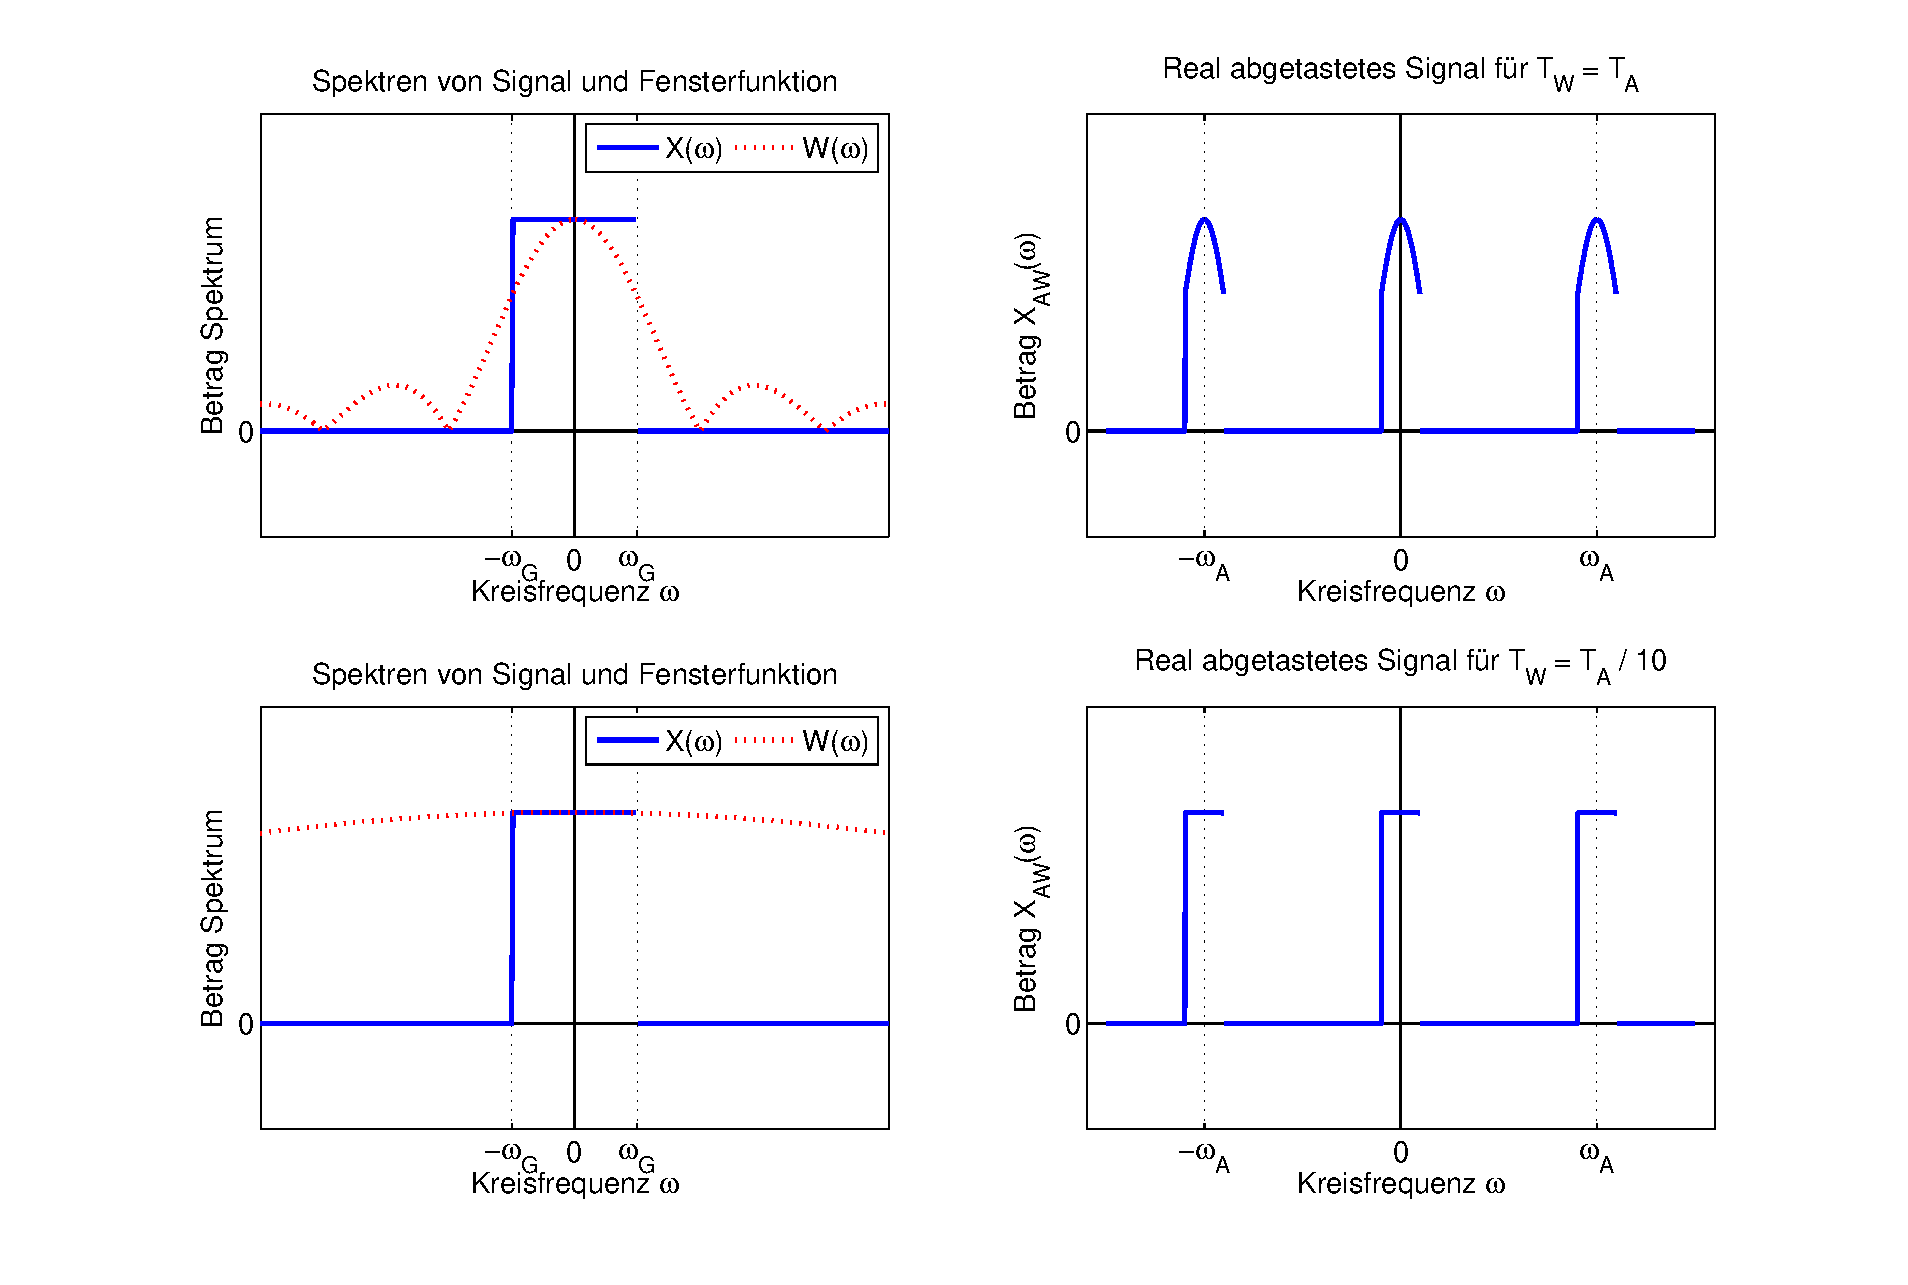
\includegraphics[width=0.5\textwidth]{Kapitel1/Bilder/image14}}
  \caption{Darstellung eines Signals x(t) und eines verst\"{a}rkten Signals 2$\cdot$ x(t)}
  \label{fig:Skalierung}
\end{figure}

\bigskip

{\fontfamily{phv}\selectfont
\noindent\textbf{Zeitliche Verschiebung}} \smallskip

\noindent Das Signal x(t - t${}_{0}$) ist gegen\"{u}ber dem Signal x(t) nach rechts (t${}_{0}$ $\mathrm{>}$ 0) beziehungsweise nach links (t${}_{0}$ $\mathrm{<}$ 0) verschoben. Bild \ref{fig:Verschiebung} zeigt ein Signal x(t) und ein um t${}_{0}$ = 5 nach rechts verschobenes Signal x(t - 5).

\begin{figure}[H]
  \centerline{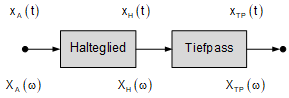
\includegraphics[width=0.5\textwidth]{Kapitel1/Bilder/image15}}
  \caption{Darstellung eines Signals x(t) und des um t${}_{0}$ = 5 nach rechts verschobenen Signals x(t - 5)}
  \label{fig:Verschiebung}
\end{figure}

\clearpage

\noindent Das Vorgehen wird am einfachsten deutlich, wenn das Argument der Funktion analysiert wird. Die Funktion x(t) weist zum Zeitpunkt t = 3 den Funktionswert 0 auf. Da in dem Zeitargument der Funktion x(t - 5) das Argument um 5 verringert wird, weist die Funktion x(t - 5) erst an der Stelle t = 8 den entsprechenden Funktionswert auf.
\bigskip

{\fontfamily{phv}\selectfont
\noindent\textbf{Zeitliche Spiegelung}} \smallskip

\noindent Die Spiegelung eines Signals x(t) an der Stelle t = 0 kann mathematisch durch den Ausdruck x(- t) dargestellt werden. Bild \ref{fig:Spiegelung} zeigt ein Signal x(t) und das gespiegelte Signal x(- t).

\begin{figure}[H]
  \centerline{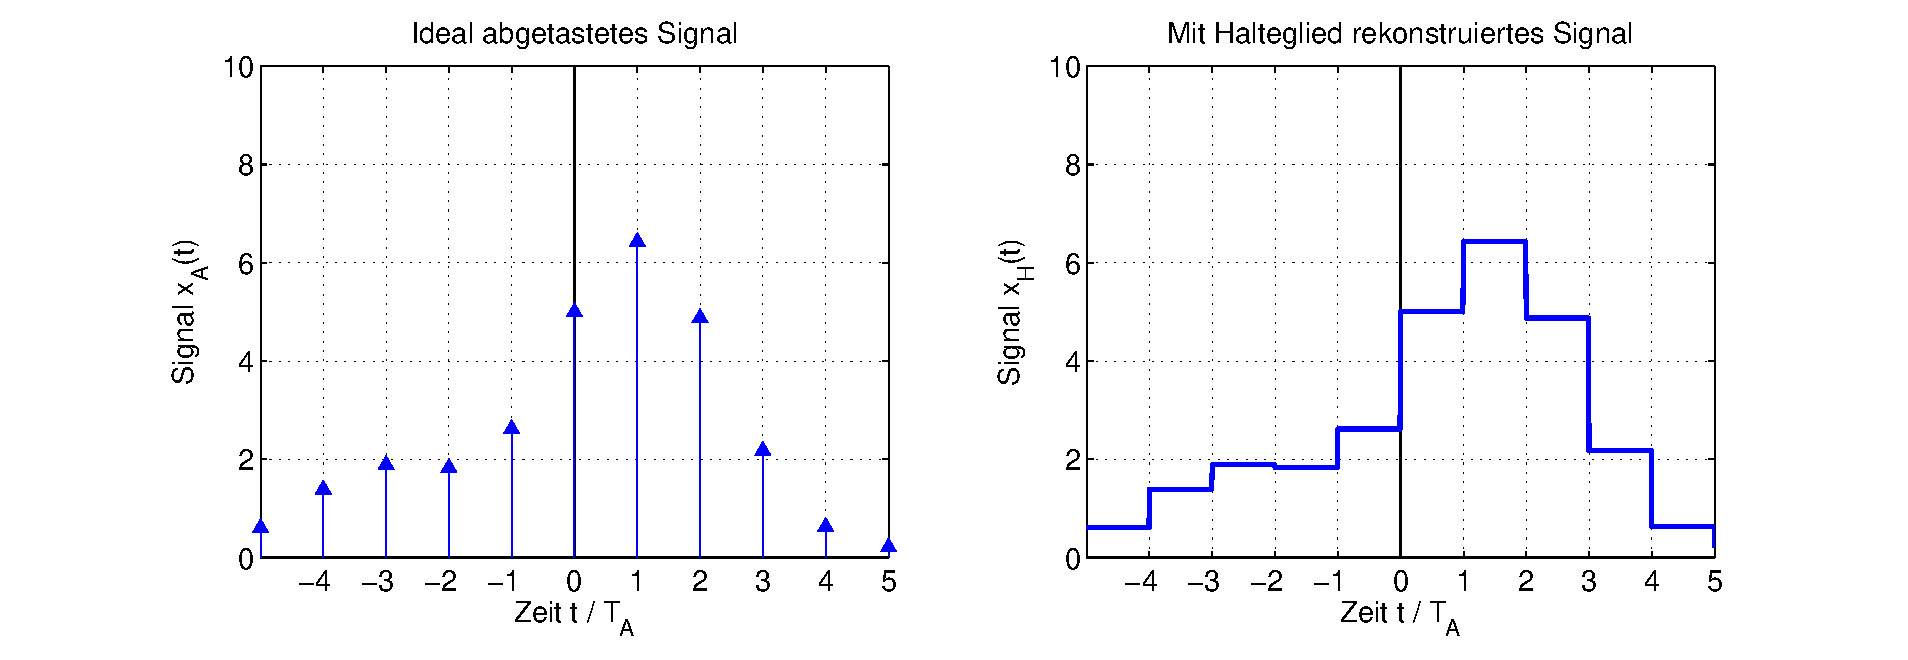
\includegraphics[width=0.5\textwidth]{Kapitel1/Bilder/image16}}
  \caption{Darstellung eines Signals x(t) und des an t = 0 gespiegelten Signals x(t)}
  \label{fig:Spiegelung}
\end{figure}

\noindent Auch hier kann das Zeitargument der Funktion analysiert werden. Die Funktion x(t) weist zum Zeitpunkt t = 1 den Funktionswert 8 auf. Die Funktion x(- t) besitzt denselben Funktionswert an der Stelle t = - 1. 

\bigskip

{\fontfamily{phv}\selectfont
\noindent\textbf{Zeitliche Skalierung}} \smallskip

\noindent Das Signal $x(a.t)$ ist gegenüber dem Signal $x(t)$ gestaucht ($a \mathrm{>} 1$) beziehungsweise gedehnt ($0 \mathrm{<} a \mathrm{<} 1$). Bild \ref{fig:Stauchung} zeigt ein Signal $x(t)$ und ein Signal $x(2.t)$.

\begin{figure}[H]
  \centerline{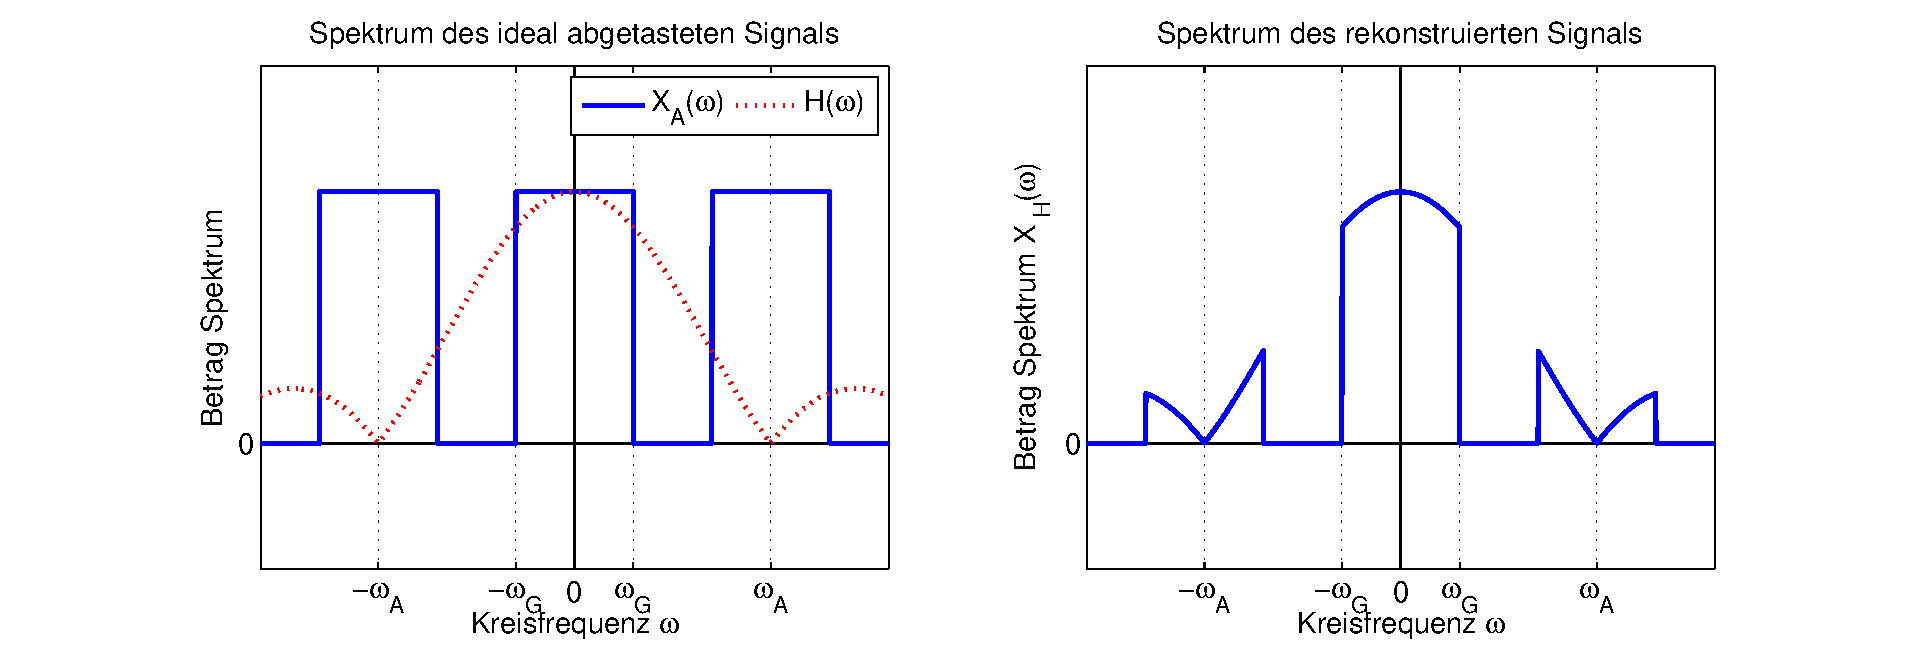
\includegraphics[width=0.5\textwidth]{Kapitel1/Bilder/image17}}
  \caption{Darstellung eines Signals x(t) und eines gestauchten Signals x(2$.$t)}
  \label{fig:Stauchung}
\end{figure}

\noindent Auch Stauchung und Dehnung werden am einfachsten deutlich, wenn das Zeitargument der Funktion x(a$.$t) analysiert wird.

\clearpage

\subsubsection{ Darstellung abschnittsweise definierter Funktionen mit Sprungfunktionen}

\noindent Die vorgestellten Sprung- und Impulsfunktionen erm\"{o}glichen in Kombination mit den vorgestellten Rechenregeln die Synthese weiterer Testfunktionen. An einem Beispiel wird das Rechnen mit Sprungfunktionen verdeutlicht. Das Signal aus Bild \ref{fig:Ueberlagerung} soll durch eine Kombination von Sprungfunktionen geschlossen also ohne Fallunterscheidung dargestellt werden.

\begin{figure}[ht]
  \centerline{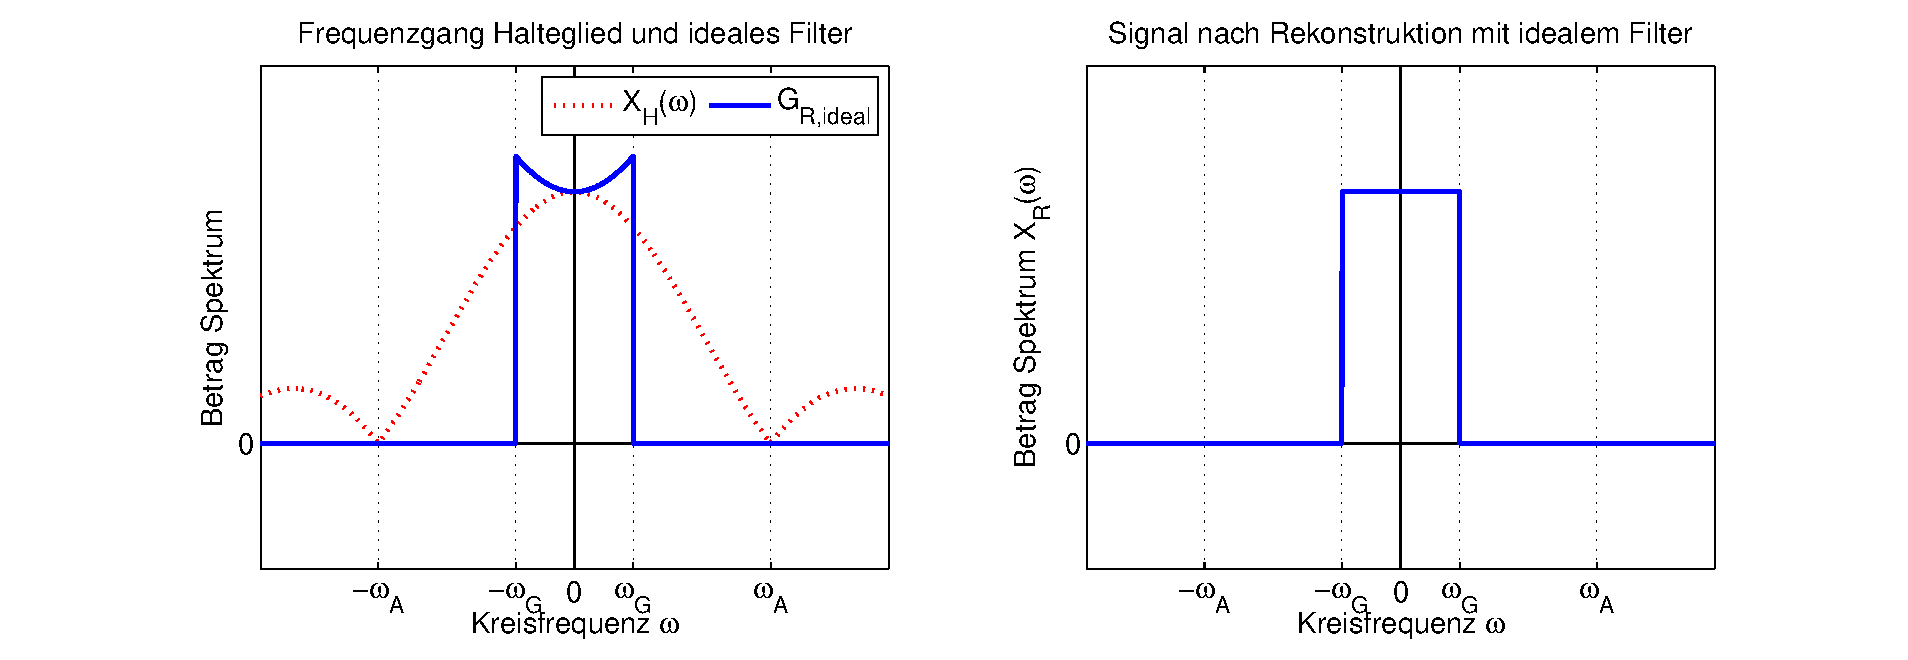
\includegraphics[width=0.5\textwidth]{Kapitel1/Bilder/image18}}
  \caption{Darstellung eines Signals x(t) als Summe von Funktionen}
  \label{fig:Ueberlagerung}
\end{figure}

\noindent Bei der Beschreibung des Signals x(t) sind insbesondere die Stellen von Bedeutung, an denen sich die Steigung des Signals \"{a}ndert. Aus Bild \ref{fig:Ueberlagerung} kann abgelesen werden, dass das die Stellen 0, T, 3$.$T, 4$.$T und 5$.$T sind.

\noindent Zum Zeitpunkt t = 0 beginnt die Funktion, mit einer Steigung 1/T zu steigen. Die Funktion x${}_{1}$(t), die dieses Verhalten beschreibt, ist die Rampenfunktion

\begin{equation}\label{eq:onefiftytwo}
x_{1} \left(t\right)=\dfrac{1}{T} \cdot t\cdot \sigma \left(t\right)
\end{equation}


\noindent Zum Zeitpunkt t = T \"{a}ndert sich die Steigung der Funktion um - 2/T. Der Faktor 2 ergibt sich dabei aus der Kompensation der vor diesem Zeitpunkt vorhandenen Steigung + 1/T und der nach dem Zeitpunkt gew\"{u}nschten Steigung - 1/T. Zu der Funktion x${}_{1}$(t) muss die Funktion x${}_{2}$(t) addiert werden, die aber erst ab dem Zeitpunkt t = T einen Einfluss haben darf. Um die Funktion f\"{u}r t $\mathrm{<}$ T auszublenden, wird die Sprungfunktion verwendet. 

\begin{equation}\label{eq:onefiftythree}
x_{2} \left(t\right)=-\dfrac{2}{T} \cdot \left(t-T\right)\cdot \sigma \left(t-T\right)
\end{equation}

\noindent Das Vorgehen wiederholt sich mit unterschiedlichen Steigungs\"{a}nderungen zu den Zeitpunkten 3$.$T, 4$.$T und 5$.$T, und es ergeben sich die Funktionen 

\begin{equation}\label{eq:onefiftyfour}
x_{3} \left(t\right)=\dfrac{1}{T} \cdot \left(t-3\cdot T\right)\cdot \sigma \left(t-3\cdot T\right)
\end{equation}

\begin{equation}\label{eq:onefiftyfive}
x_{4} \left(t\right)=\dfrac{1}{T} \cdot \left(t-4\cdot T\right)\cdot \sigma \left(t-4\cdot T\right)
\end{equation}


\begin{equation}\label{eq:onefiftysix}
x_{5} \left(t\right)=-\dfrac{1}{T} \cdot \left(t-5\cdot T\right)\cdot \sigma \left(t-5\cdot T\right)
\end{equation}

\noindent Das Signal x(t) kann damit als \"{U}berlagerung der Teilfunktionen x${}_{1}$(t) bis x${}_{5}$(t) dargestellt werden.


\begin{equation}\label{eq:onefiftyseven}
\begin{split}
x(t) & = \dfrac{t}{T} \cdot \sigma \left(t\right)-2\cdot \dfrac{t-T}{T} \cdot \sigma \left(t-T\right)+\dfrac{t-3\cdot T}{T} \cdot \sigma \left(t-3\cdot T\right) \\
 & +\dfrac{t-4\cdot T}{T} \cdot \sigma \left(t-4\cdot T\right)-\dfrac{t-5\cdot T}{T} \cdot \sigma \left(t-5\cdot T\right)
\end{split}
\end{equation}


\noindent Durch den Einsatz der Sprungfunktionen ist gew\"{a}hrleistet, dass die Funktion erst ab einem definierten Zeitpunkt wirkt. Sprungfunktionen erm\"{o}glichen damit die sukzessive Synthese des Signals x(t). 


\subsubsection{ Verallgemeinerte Ableitung}

\noindent Die klassischen Differentiationsregeln erlauben die Berechnung von Ableitungen f\"{u}r stetige Funktionen. In der Systemtheorie werden aber Testfunktionen eingesetzt, die an einer oder mehreren Stellen Spr\"{u}nge aufweisen k\"{o}nnen. Um auch f\"{u}r diese Funktionen Ableitungen angeben zu k\"{o}nnen, wird ein Vorgehen zur Bestimmung einer verallgemeinerten Ableitung von Funktionen mit Spr\"{u}ngen definiert. Dazu wird die Funktion mit einem Sprung an der Stelle t = t${}_{0}$ in eine stetige Funktion x${}_{S}$(t) und einen idealen Sprung der H\"{o}he $\Delta$x an der Stelle t${}_{0}$ zerlegt.

\begin{figure}[ht]
  \centerline{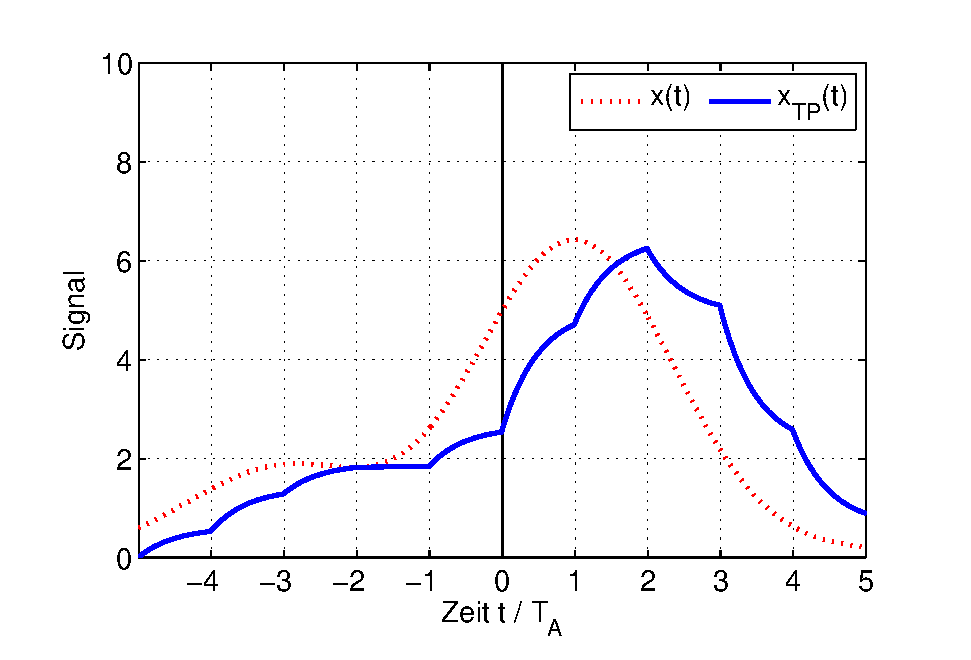
\includegraphics[width=0.5\textwidth]{Kapitel1/Bilder/image19}}
  \caption{Zerlegung der Funktion x(t) in einen stetigen Anteil x${}_{S}$(t) und einen idealen Sprung der H\"{o}he $\Delta$x}
  \label{fig:DifferenzierenErweitert}
\end{figure}
\noindent Die H\"{o}he $\Delta$x des Sprungs ergibt sich aus der Differenz des rechtsseitigen Grenzwertes x(t${}_{0+}$) und linksseitigen Grenzwertes x(t${}_{0-}$) zu 

\begin{equation}\label{eq:onefiftyeight}
\Delta x=x\left(t_{0+} \right)-x\left(t_{0-} \right)
\end{equation}


\noindent Aufgrund der Linearit\"{a}t der Ableitungsoperation und der Ableitung der Sprungfunktion 
\begin{equation}\label{eq:onefiftynine}
\dfrac{d\sigma }{dt} =\delta \left(t\right)
\end{equation}

\noindent errechnet sich die Ableitung der Funktion x(t) zu

\begin{equation}\label{eq:onesixty}
\begin{split}
 \dfrac{dx}{dt}  & =  \dfrac{dx_{S}}{dt} +\dfrac{d}{dt} \left(\sigma \left(t-t_{0} \right)\cdot \left(x\left(t_{0+} \right)-x\left(t_{0-} \right)\right)\right) = \dfrac{dx_{S} }{dt} +\dfrac{d}{dt} \left(\sigma \left(t-t_{0} \right)\cdot \Delta x\right) \\
 & = \dfrac{dx_{S} }{dt} +\delta \left(t-t_{0} \right)\cdot \Delta x 
\end{split}
\end{equation}


\noindent Die verallgemeinerte Ableitung ergibt sich damit aus der Ableitung der stetigen Funktion x${}_{S}$(t) und einem Impuls an der Sprungstelle t${}_{0}$ mit dem Gewicht der Sprungh\"{o}he $\Delta$x. Im Folgenden wird bei der zeitlichen Ableitung immer die verallgemeinerte zeitliche Ableitung angewendet. \clearpage

\noindent
\colorbox{lightgray}{%
\arrayrulecolor{white}%
\renewcommand\arraystretch{0.6}%
\begin{tabular}{ wl{16.5cm} }
{\fontfamily{phv}\selectfont
\noindent{Beispiel: Funktionsalgebra}} 
\end{tabular}%
}\bigskip

\noindent Gegeben ist folgender Signalverlauf x(t). F\"{u}r t $\mathrm{>}$ 6 hat das Signal den Wert null.

\begin{figure}[H]
  \centerline{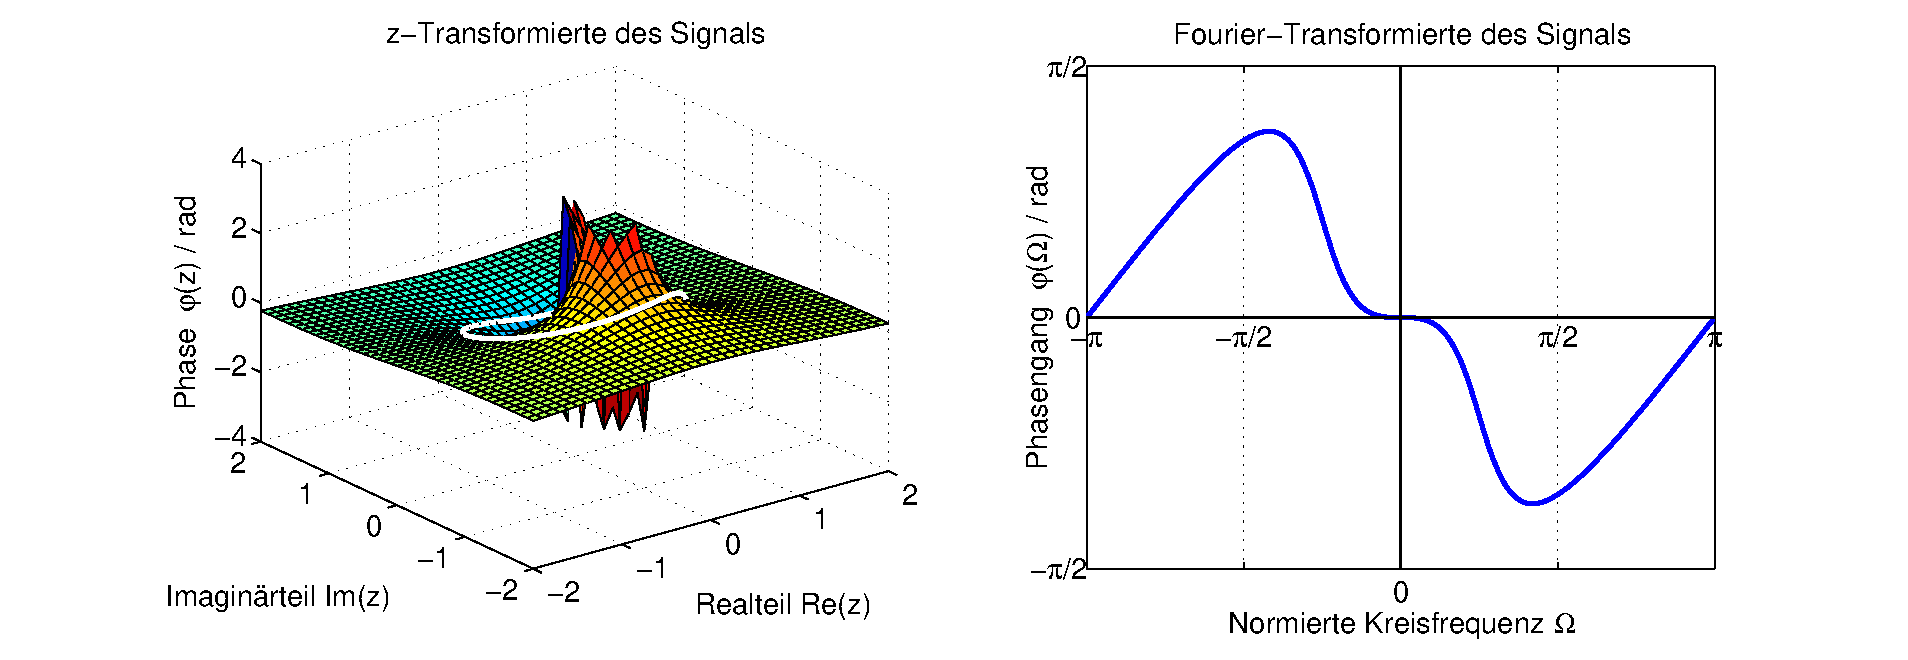
\includegraphics[width=0.8\textwidth]{Kapitel1/Bilder/image20}}
  \caption{Signalverlauf eines Signals x(t) und verallgemeinerte Ableitung des Signalverlaufs}
  \label{fig:BeispielFunktionsalgebra}
\end{figure}

\noindent Das Signal setzt sich aus einem Sprung an der Stelle t = 0, einer Rampe mit negativer Steigung beginnend an der Stelle t = 1 zusammen. Die negative Steigung wird an der Stelle t = 3 kompensiert, an der Stelle t = 5 weist das Signal einen positiven Sprung auf. Mathematisch ergibt sich


\begin{equation}\label{eq:onesixtyone}
x\left(t\right)=\sigma \left(t\right)-\left(t-1\right)\cdot \sigma \left(t-1\right)+\left(t-3\right)\cdot \sigma \left(t-3\right)+\sigma \left(t-5\right)
\end{equation}

\noindent Die Ableitung des Signals erfolgt nach den Rechenregeln der Differentiation mit dem Zusatz der Ableitung von Spr\"{u}ngen. Mit der Produktregel der Differentiation ergibt sich

\begin{equation}\label{eq:onesixtytwo}
\dfrac{dx}{dt} =\delta \left(t\right)-\left(\left(t-1\right)\cdot \delta \left(t-1\right)+\sigma \left(t-1\right)\right)+\left(\left(t-3\right)\cdot \delta \left(t-3\right)+\sigma \left(t-3\right)\right)+\delta \left(t-5\right)
\end{equation}

\noindent In dem Ausdruck treten Terme der Form 

\begin{equation}\label{eq:onesixtythree}
y\left(t\right)=\left(t-t_{0} \right)\cdot \delta \left(t-t_{0} \right)=0
\end{equation}

\noindent auf. Da immer einer der beiden Faktoren null ist, ist das Produkt insgesamt null. Damit kann die Ableitung vereinfacht werden zu 

\begin{equation}\label{eq:onesixtyfour}
\dfrac{dx}{dt} =\delta \left(t\right)-\sigma \left(t-1\right)+\sigma \left(t-3\right)+\delta \left(t-5\right)
\end{equation}

\noindent Die verallgemeinerte Ableitung ist in Bild \ref{fig:BeispielFunktionsalgebra} rechts dargestellt.

\noindent 
\noindent
\noindent


\InsertBoxL{0}{
\includegraphics[scale=0.5]{Code.JPG}} 
\textcolor{white}{.}\newline
\noindent Im Online-Portal \textit{Systemtheorie Online} verdeutlicht die Applikation \textit{Komplexe Exponentialfunktion} den Zusammenhang zwischen der Lage des Wertes $\lambda = \delta + j.\omega{}_{0}$ in der komplexen Ebene und dem Verhalten der Schwingung.\newline


\noindent 


\subsubsection{ Zusammenfassung Funktionsalgebra}

\noindent In Tabelle \ref{tab:twofour} sind die besprochenen Rechenregeln zusammengefasst. Die Anwendung dieser Regeln ist die Zerlegung von Signalen in bekannte Signale. Das Rechnen mit Funktionen ist Grundlage für eine erfolgreiche Anwendung von Korrespondenztafeln der Laplace- und Fourier-Transformation, die in Kapitel 4 und 6 beschrieben werden 

\clearpage

\begin{table}[H]
\setlength{\arrayrulewidth}{.1em}
\caption{Tabellarische Zusammenfassung von Testfunktionen}
\setlength{\fboxsep}{0pt}%
\colorbox{lightgray}{%
\arrayrulecolor{white}%
\begin{tabular}{| l | l |}
\hline
\parbox[c][0.28in][c]{3.3in}{\smallskip\centering\textbf{\fontfamily{phv}\selectfont{Testfunktion}}} & \parbox[c][0.28in][c]{3.3in}{\smallskip\centering\textbf{\fontfamily{phv}\selectfont{Mathematische Beschreibung}}}\\ \hline

\parbox[c][0.64in][c]{3.3in}{\centering{\fontfamily{phv}\selectfont{Skalierung der Amplitude}}} & 
\parbox[c][0.64in][c]{3.3in}{\centering{$y\left(t\right)=a\cdot x\left(t\right)$}}\\ \hline

\parbox[c][0.64in][c]{3.3in}{\centering{\fontfamily{phv}\selectfont{Zeitliche Verschiebung um $t{}_{0}$}}} & \parbox[c][0.64in][c]{3.3in}{\centering{$y\left(t\right)=x\left(t-t_{0} \right)$}}\\ \hline

\parbox[c][0.64in][c]{3.3in}{\centering{\fontfamily{phv}\selectfont{Zeitliche Spiegelung}}} & 
\parbox[c][0.64in][c]{3.3in}{\centering{$y\left(t\right)=x\left(-t\right)$}}\\ \hline

\parbox[c][0.64in][c]{3.3in}{\centering{\fontfamily{phv}\selectfont{Zeitliche Skalierung}}} & 
\parbox[c][0.64in][c]{3.3in}{\centering{$y\left(t\right)=x\left(a\cdot t\right)$}}\\ \hline

\parbox[c][0.64in][c]{3.3in}{\centering{\fontfamily{phv}\selectfont{Verallgemeinerte Ableitung einer Funktion x(t)mit Sprung $\Delta$x an der Stelle $t{}_{0}$}}} &
\parbox[c][0.64in][c]{3.3in}{\centering{$\dfrac{dx}{dt} =\dfrac{dx_{S} }{dt} +\delta \left(t-t_{0} \right)\cdot \Delta x$}}\\ \hline

\end{tabular}%
}
\label{tab:twofour}
\end{table}

\clearpage 


\subsection{ Funktionen zur Beschreibung von Einschwingvorg\"{a}ngen}


\subsubsection{ Periodische und harmonische Funktionen}

Periodische Funktionen sind dadurch gekennzeichnet, dass sich der Funktionswert periodisch nach einer Zeitdauer T${}_{0}$ wiederholt. Bild \ref{fig:Periodisch} zeigt ein einfaches periodisches Signal.

\begin{figure}[ht]
  \centerline{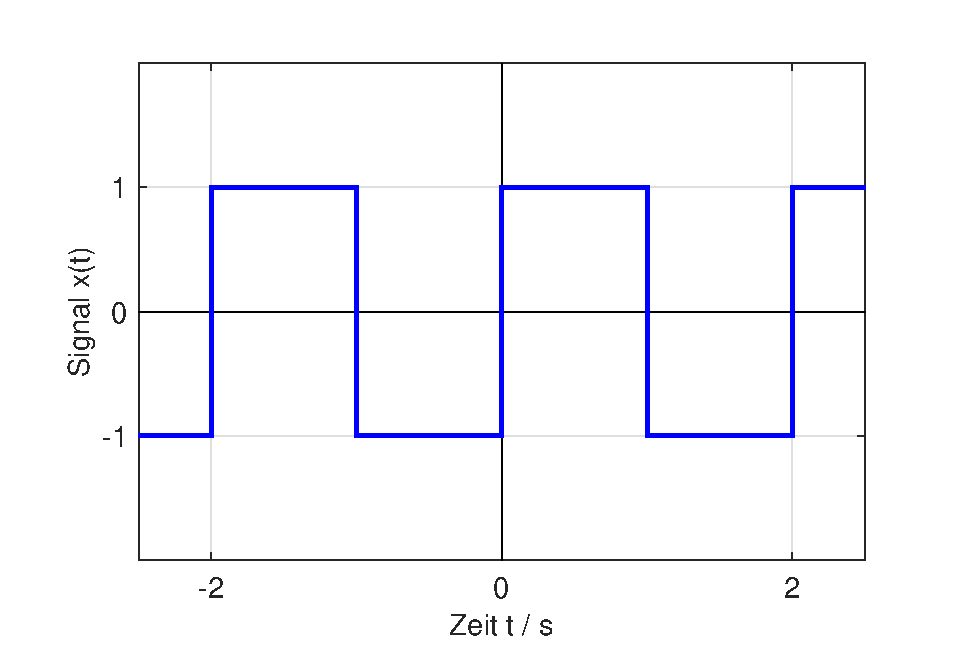
\includegraphics[width=0.5\textwidth]{Kapitel1/Bilder/image21}}
  \caption{Beispiel f\"{u}r ein periodisches Signal mit einer Periodendauer T${}_{0}$ = 2 s }
  \label{fig:Periodisch}
\end{figure}

\noindent F\"{u}r periodische Funktionen und ganzzahlige Werte k gilt:

\begin{equation}\label{eq:onesixtyfive}
x\left(t\right)=x\left(t+k\cdot T_{0} \right)
\end{equation}

\noindent Neben den bereits diskutierten Testfunktionen, die das Ein-, Aus- oder Umschalten modellieren, sind in der Systemtheorie periodische, harmonische Signale von gro{\ss}er Bedeutung. Als Beispiel soll hier eine Kosinusfunktion diskutiert werden. Sie ist definiert als

\begin{equation}\label{eq:onesixtysix}
x\left(t\right)=A\cdot \cos \left(\omega _{0} \cdot t+\varphi \right)=A\cdot \cos \left(\omega _{0} \cdot \left(t+t_{0} \right)\right)
\end{equation}

\noindent mit

\begin{equation}\label{eq:onesixtyseven}
t_{0} =\dfrac{\varphi }{\omega _{0} } 
\end{equation}

\noindent wobei A die Amplitude der Schwingung, $\varphi$ der Nullphasenwinkel und $\omega{}_{0}$ die Kreisfrequenz ist.

\begin{equation}\label{eq:onesixtyeight}
\omega _{0} =\dfrac{2\cdot \pi }{T_{0} } =2\cdot \pi \cdot f_{0} 
\end{equation}

\noindent Die Frequenz f${}_{0}$ der Funktion x(t) ist der Kehrwert der Periodendauer T${}_{0}$ der Schwingung.

\begin{equation}\label{eq:onesixtynine}
f_{0} =\dfrac{1}{T_{0} } =\dfrac{\omega _{0} }{2\cdot \pi }
\end{equation}

\clearpage
\noindent Bild \ref{fig:Inconnue} verdeutlicht diese Definitionen an einem Beispiel:

\begin{figure}[ht]
  \centerline{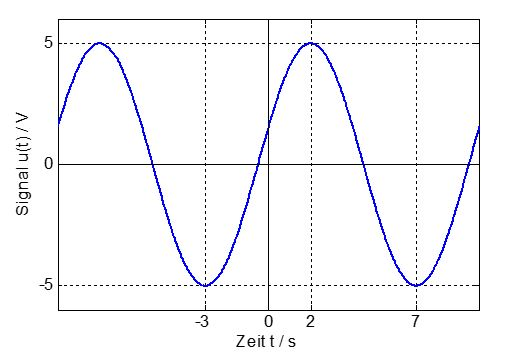
\includegraphics[width=0.5\textwidth]{Kapitel1/Bilder/image22.JPG}}
  \caption{Kosinusfunktion mit einer Periodendauer T${}_{0}$ = 10 s, einer Amplitude von 5 V und einem Nullphasenwinkel von - 2/5$.$$\pi$ }
  \label{fig:Inconnue}
\end{figure}

\noindent In dem Beispiel beträgt die Amplitude 5 V. Die Kosinusfunktion hat zwei aufeinanderfolgende Minima bei t = - 3 s und t = 7 s, woraus sich eine Periodendauer von T${}_{0}$ = 10 s ergibt. Die Nullphase $\varphi$ ist nicht unmittelbar aus dem Diagramm ablesbar. Die Kosinusfunktion ist in Bild 2.22 um 2 s nach rechts verschoben. Es liegt demnach eine zeitliche Verz\"{o}gerung von t${}_{0}$ = - 2 s vor. \"{U}ber den Zusammenhang

\begin{equation}\label{eq:oneseventy}
t_{0} =\dfrac{\varphi }{2\cdot \pi \cdot f_{0} } =\dfrac{\varphi }{2\cdot \pi } \cdot T_{0} =-2 \; s
\end{equation}


\noindent kann der Nullphasenwinkel $\varphi$ berechnet werden zu

\begin{equation}\label{eq:oneseventyone}
\varphi =-\dfrac{2\cdot \pi \cdot 2\;s}{10\;s} =-\dfrac{2\cdot \pi }{5}
\end{equation}

\bigskip

{\fontfamily{phv}\selectfont
\noindent\textbf{\"{U}berlagerung harmonischer Signale}} \smallskip

\noindent Harmonische Signale mit Nullphasenwinkel k\"{o}nnen mithilfe der Additionstheoreme als Summe von einer Sinus- und einer Kosinusfunktion dargestellt werden.

\begin{equation}\label{eq:oneseventytwo}
\sin \left(a+b\right)=\sin \left(a\right)\cdot \cos \left(b\right)+\cos \left(a\right)\cdot \sin \left(b\right)
\end{equation}


\begin{equation}\label{eq:oneseventythree}
\sin \left(a-b\right)=\sin \left(a\right)\cdot \cos \left(b\right)-\cos \left(a\right)\cdot \sin \left(b\right)
\end{equation}


\begin{equation}\label{eq:oneseventyfour}
\cos \left(a+b\right)=\cos \left(a\right)\cdot \cos \left(b\right)-\sin \left(a\right)\cdot \sin \left(b\right)
\end{equation}

\begin{equation}\label{eq:oneseventyfive}
\cos \left(a-b\right)=\cos \left(a\right)\cdot \cos \left(b\right)+\sin \left(a\right)\cdot \sin \left(b\right)
\end{equation}

\noindent Eine Kosinusfunktion mit dem Nullphasenwinkel $\varphi$ kann also als Summe einer Kosinus- und Sinusfunktion mit Nullphasenwinkel $\varphi$ = 0 dargestellt werden.

\begin{equation}\label{eq:oneseventysix}
\begin{split}
x(t) & = A\cdot \cos \left(\omega _{0} \cdot t+\varphi \right) \\ 
 & = A\cdot \cos \left(\omega _{0} \cdot t\right)\cdot \cos \left(\varphi \right)-A\cdot \sin \left(\omega _{0} \cdot t\right)\cdot \sin \left(\varphi \right) \\
 & = a\cdot \cos \left(\omega _{0} \cdot t\right)-b\cdot \sin \left(\omega _{0} \cdot t\right)
\end{split}
\end{equation}

\noindent wobei sich deren Amplituden durch einen Koeffizientenvergleich ergeben zu 

\begin{equation}\label{eq:oneseventyseven}
a=A\cdot \cos \left(\varphi \right)
\end{equation}


\begin{equation}\label{eq:oneseventyeight}
b=A\cdot \sin \left(\varphi \right)
\end{equation}

\noindent Umgekehrt k\"{o}nnen eine Kosinus- und eine Sinusfunktion gleicher Frequenz addiert werden zu einer resultierenden Schwingung mit Amplitude A und Nullphasenwinkel $\varphi$:

\begin{equation}\label{eq:oneseventynine}
\begin{split}
x\left(t\right) & = a\cdot \cos \left(\omega _{0} \cdot t\right)-b\cdot \sin \left(\omega _{0} \cdot t\right) \\ 
& = A\cdot \cos \left(\varphi \right)\cdot \cos \left(\omega _{0} \cdot t\right)-A\cdot \sin \left(\varphi \right)\cdot \sin \left(\omega _{0} \cdot t\right) \\ 
& = A\cdot \cos \left(\omega _{0} \cdot t+\varphi \right)    
\end{split}
\end{equation}


\noindent Dabei ergeben sich Amplitude und Nullphasenwinkel aus 

\begin{equation}\label{eq:oneeighty}
A=\sqrt{a^{2} +b^{2} } 
\end{equation}

\begin{equation}\label{eq:oneeightyone}
\tan \left(\varphi \right)=\dfrac{\sin \left(\varphi \right)}{\cos \left(\varphi \right)} =\dfrac{b}{a} 
\end{equation}

\noindent Aus einer \"{U}berlagerung von Sinus- und Kosinusfunktionen gleicher Frequenz resultiert eine Sinus- oder Kosinusfunktion mit derselben Frequenz, aber unterschiedlicher Amplitude und Nullphase.\bigskip

{\fontfamily{phv}\selectfont
\noindent\textbf{Zeigerdarstellung harmonischer Signalen}} \smallskip

\noindent In der Elektrotechnik hat sich f\"{u}r die Berechnung von harmonisch angeregten Schaltungen die Zeigerdarstellung durchgesetzt. Sie beruht auf der Eulerschen Formel.

\begin{equation}\label{eq:oneeightytwo}
e^{j\cdot \varphi } =\cos \left(\varphi \right)+j\cdot \sin \left(\varphi \right)
\end{equation}


\noindent Damit kann eine Kosinusfunktion der Form

\begin{equation}\label{eq:oneeightythree}
x\left(t\right)=A\cdot \cos \left(\omega _{0} \cdot t+\varphi \right)
\end{equation}


\noindent als Realteil einer komplexen Funktion

\begin{equation}\label{eq:oneeightyfour}
z\left(t\right)=A\cdot e^{j\cdot \left(\omega _{0} \cdot t+\varphi \right)} =A\cdot e^{j\cdot \varphi } \cdot e^{j\cdot \omega _{0} \cdot t} =A\cdot \left(\cos \left(\omega _{0} \cdot t+\varphi \right)+j\cdot \sin \left(\omega _{0} \cdot t+\varphi \right)\right)
\end{equation}


\noindent aufgefasst werden. Diese mathematische Darstellung kann durch einen Zeiger der L\"{a}nge A verdeutlicht werden, der in der komplexen Ebene um den Koordinatenursprung rotiert. Die Zeit f\"{u}r eine volle Umdrehung ist die Periodendauer T${}_{0}$. Die eigentlich interessierende Gr\"{o}{\ss}e ist die Projektion des Zeigers auf die reelle Achse, sie stellt die Funktion x(t) dar. Zum Zeitpunkt t = 0 gilt

\begin{equation}\label{eq:oneeightyfive}
z\left(0\right)=A\cdot e^{j\cdot \varphi } =A\cdot \cos \left(\varphi \right)+j\cdot A\cdot \sin \left(\varphi \right)=\underline{A}
\end{equation}

\noindent \underbar{A} wird als komplexe Amplitude der komplexen Funktion z(t) bezeichnet. Ein Vergleich der Koeffizienten mit Gleichung \ref{eq:oneseventysix} zeigt, dass die komplexe Amplitude \underbar{A} dargestellt werden kann, als 

\begin{equation}\label{eq:oneeightysix}
\underline{A}=a+j\cdot b
\end{equation}


\noindent Zur Verdeutlichung der komplexen Amplitude \underbar{A} zeigt Bild \ref{fig:HarmonischeSchwingung} eine Zeigerdarstellung in der komplexen Ebene. Sie illustriert die Projektion des komplexen Zeigers auf die reelle Achse als Zeitfunktion x(t).

\noindent 
\begin{figure}[H]
  \centerline{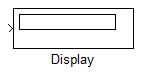
\includegraphics[width=0.45\textwidth]{Kapitel1/Bilder/image23}}
  \caption{Darstellung einer harmonischen Schwingung als Zeigerdiagramm }
  \label{fig:HarmonischeSchwingung}
\end{figure}

\medskip
{\fontfamily{phv}\selectfont
\noindent\textbf{Darstellung harmonischer Signale als Überlagerung komplexer Schwingungen}} \smallskip

\noindent Durch Umformung von Gleichung \ref{eq:oneeightytwo} ergibt sich f\"{u}r Sinus- und Kosinusfunktionen die Darstellung


\begin{equation}\label{eq:oneeightyseven}
\cos \left(\varphi \right)=\dfrac{1}{2} \cdot \left(e^{j\cdot \varphi } +e^{-j\cdot \varphi } \right)
\end{equation}

\begin{equation}\label{eq:oneeightyeight}
\sin \left(\varphi \right)=\dfrac{1}{2\cdot j} \cdot \left(e^{j\cdot \varphi } -e^{-j\cdot \varphi } \right)=-\dfrac{1}{2} \cdot j\cdot \left(e^{j\cdot \varphi } -e^{-j\cdot \varphi } \right)
\end{equation}


\noindent Werden in Gleichung \ref{eq:oneseventynine} die reellen Sinus- und Kosinusfunktionen durch Summen komplexer Funktionen nach Gleichung \ref{eq:oneeightyseven} und \ref{eq:oneeightyeight} ersetzt, so ergibt sich 

\begin{equation}\label{eq:oneeightynine}
\begin{split}
x(t) & = a\cdot \cos \left(\omega _{0} \cdot t\right)-b\cdot \sin \left(\omega _{0} \cdot t\right) \\ 
 & = a\cdot \dfrac{1}{2} \cdot \left(e^{j\cdot \omega _{0} \cdot t} +e^{-j\cdot \omega _{0} \cdot t} \right)-b\cdot \dfrac{1}{2\cdot j} \cdot \left(e^{j\cdot \omega _{0} \cdot t} -e^{-j\cdot \omega _{0} \cdot t} \right) \\ 
 & = \dfrac{1}{2} \cdot \left(a+j\cdot b\right)\cdot e^{j\cdot \omega _{0} \cdot t} +\dfrac{1}{2} \cdot \left(a-j\cdot b\right)\cdot e^{-j\cdot \omega _{0} \cdot t } 
\end{split}
\end{equation}


\noindent Der erste Summand beschreibt einen komplexen Zeiger, der sich in der komplexen Ebene mit einer Periodendauer T${}_{0}$ in mathematisch positiver Richtung dreht. Der zweite Summand beschreibt einen zweiten komplexen Zeiger, der zu jedem Zeitpunkt konjugiert komplex zum Ersten ist. Er dreht sich mit derselben Winkelgeschwindigkeit wie der erste Zeiger, aber in entgegengesetzter Richtung. 

\noindent Aus den komplexen Koeffizienten 

\begin{equation}\label{eq:oneninety}
\underline{c}=\dfrac{a+j\cdot b}{2}
\end{equation}

\begin{equation}\label{eq:oneninetyone}
\underline{c}*=\dfrac{a-j\cdot b}{2}
\end{equation}

\noindent errechnen sich die Amplitude A und der Nullphasenwinkel $\varphi$ zu

\begin{equation}\label{eq:oneninetytwo}
A=2\cdot \left|\underline{c}\right|
\end{equation}

\begin{equation}\label{eq:oneninetythree}
\varphi =\arg \left(\underline{c}\right)
\end{equation}

\noindent Die komplexe Exponentialfunktion stellt reelle Funktionen mithilfe komplexer Zahlen dar. Es ist eine effiziente Beschreibungsform, die gleicherma{\ss}en Amplitude und Phase beschreibt. Physikalisch gesehen existieren komplexe Signale nicht.

\noindent
\noindent

%%%%%%%%%%%%%% CODE BILD

\clearpage


\subsubsection{ Exponentialfunktion}

\noindent Bei der Diskussion von Systemen wird sich zeigen, dass die Exponentialfunktion 

\begin{equation}\label{eq:oneninetyfour}
x\left(t\right)=A\cdot e^{\lambda \cdot t} \cdot \sigma \left(t\right)
\end{equation}

 
\noindent die Einschwingvorgänge vieler physikalischer Vorgänge beschreiben kann. Bild \ref{fig:Exponentialfunktion} stellt das Verhalten der Exponentialfunktion für unterschiedliche reelle Parameter $\lambda$ im Zeitraum t $\mathrm{>}$ 0 dar.

\begin{figure}[ht]
  \centerline{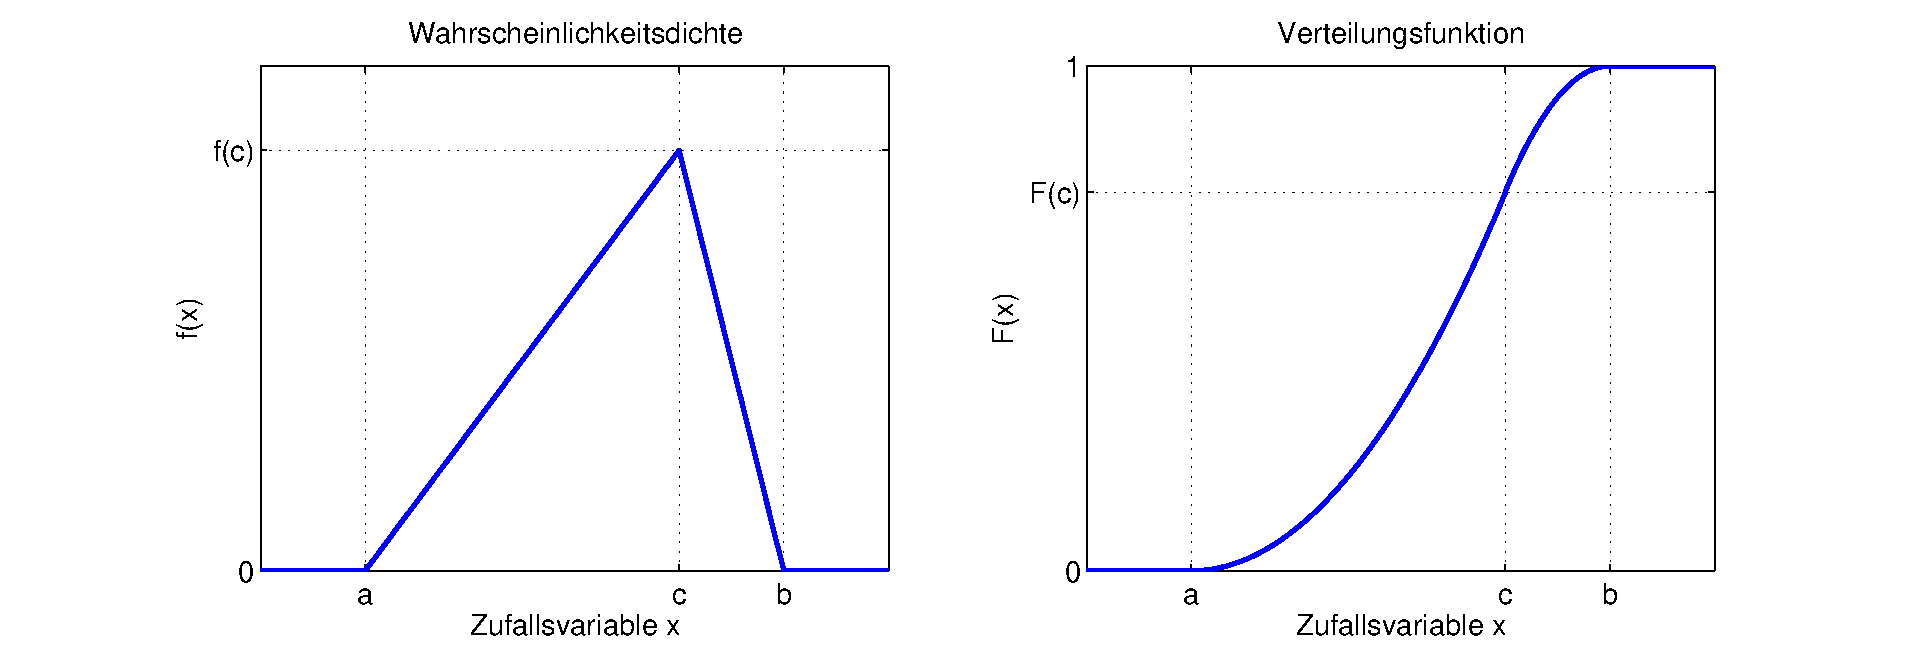
\includegraphics[width=0.5\textwidth]{Kapitel1/Bilder/image24}}
  \caption{Darstellung der Exponentialfunktion f\"{u}r unterschiedliche Parameter $\lambda$ }
  \label{fig:Exponentialfunktion}
\end{figure}

\noindent Die Exponentialfunktion beginnt f\"{u}r alle Parameter $\lambda$ an der Stelle x(t = 0) = A. F\"{u}r reelle Parameter $\lambda$ $\mathrm{>}$ 0 steigt die Exponentialfunktion mit wachsender Zeit t. Bei negativem reellen Parameter $\lambda$ $\mathrm{<}$ 0 n\"{a}hert sich die Exponentialfunktion der Asymptote x = 0. F\"{u}r $\lambda$ = 0 bleibt die Exponentialfunktion konstant bei x = A.

\noindent Im vorangegangenen Abschnitt wird auf Exponentialfunktionen mit rein imagin\"{a}ren Werten von $\lambda$ verwiesen, und es wird aufgezeigt, dass sie harmonische Schwingungen beschreiben k\"{o}nnen. Au{\ss}er reellen und imagin\"{a}ren Argumenten k\"{o}nnen bei Exponentialfunktionen auch komplexe Argumente $\lambda$ auftreten. In diesem Fall kann die Exponentialfunktion in zwei Faktoren zerlegt werden:

\begin{equation}\label{eq:oneninetyfive}
e^{\lambda \cdot t} =e^{\left(\delta _{0} +j\cdot \omega _{0} \right)\cdot t} =e^{\delta _{0} \cdot t} \cdot e^{j\cdot \omega _{0} \cdot t}
\end{equation}

\noindent Damit kann eine Kosinusfunktion mit exponentiell abklingender Amplitude als Summe zweier Exponentialfunktionen mit jeweils konjugiert komplexen Koeffizienten $\lambda$ dargestellt werden. 

\begin{equation}\label{eq:oneninetysix}
\begin{split}
x(t) & ={A\cdot e^{\delta _{0} \cdot t} \cdot \cos \left(\omega _{0} \cdot t\right)\cdot \sigma \left(t\right)=\dfrac{1}{2} \cdot A\cdot e^{\delta _{0} \cdot t} \cdot \left(e^{j\cdot \omega _{0} \cdot t} +e^{-j\cdot \omega _{0} \cdot t} \right)\cdot \sigma \left(t\right)} \\
& = \dfrac{1}{2} \cdot A\cdot \left(e^{\left(\delta _{0} +j\cdot \omega _{0} \right)\cdot t} +e^{\left(\delta _{0} -j\cdot \omega _{0} \right)\cdot t} \right)\cdot \sigma \left(t\right)    
\end{split}
\end{equation}


\noindent Die Kosinusfunktion mit exponentiell abklingender Amplitude ist in Bild \ref{fig:KomplexExponentialfunktion} dargestellt. Dabei sind die Einh\"{u}llenden der Kosinusfunktion als gestrichelte Linie eingezeichnet.

\clearpage
\begin{figure}[H]
  \centerline{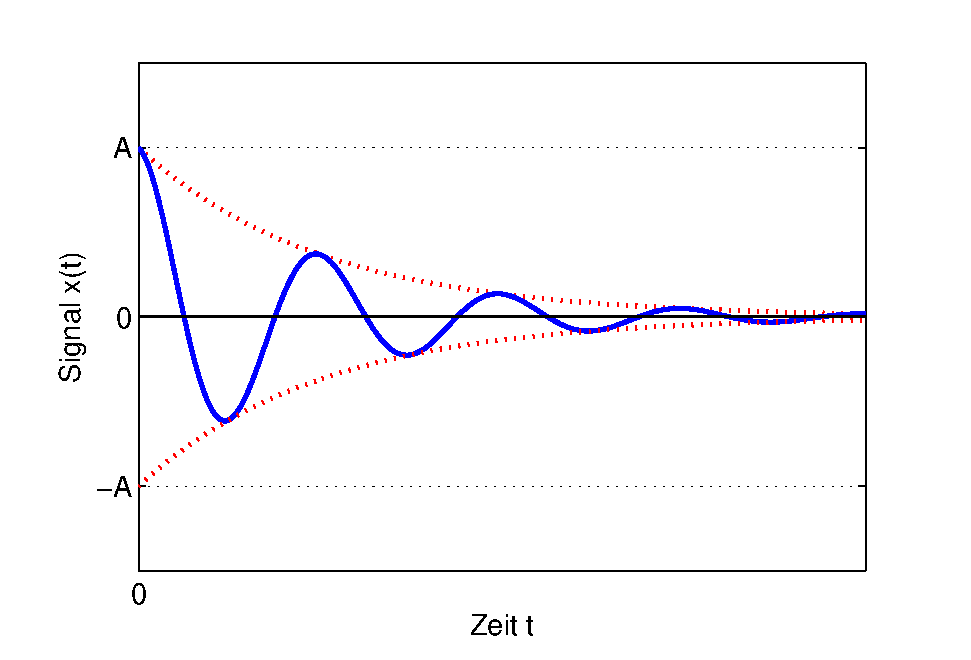
\includegraphics[width=0.5\textwidth]{Kapitel1/Bilder/image25}}
  \caption{Darstellung einer Exponentialfunktion mit abklingender Amplitude}
  \label{fig:KomplexExponentialfunktion}
\end{figure}

\noindent Bild \ref{fig:KomplexExponentialfunktion3D} zeigt eine r\"{a}umliche Darstellung der komplexen Exponentialfunktion und die Projektion der Funktion auf die Realteil-Zeit-Ebene.

\begin{figure}[H]
  \centerline{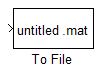
\includegraphics[width=0.5\textwidth]{Kapitel1/Bilder/image26}}
  \caption{R\"{a}umliche Darstellung der komplexen Exponentialfunktion und Projektion der Funktion auf die Realteil-Zeit-Ebene}
  \label{fig:KomplexExponentialfunktion3D}
\end{figure}

\noindent Die Projektion der komplexen Exponentialfunktion auf die Realteil-Zeit-Ebene ergibt die abklingende harmonische Schwingung.

\begin{equation}\label{eq:oneninetyseven}
x\left(t\right)=A\cdot e^{\delta _{0} \cdot t} \cdot \cos \left(\omega _{0} \cdot t\right)\cdot \sigma \left(t\right)
\end{equation}

\noindent Je nach Lage des Wertes $\lambda = \delta{}_{0} + j.\omega{}_{0}$ in der komplexen Ebene, ergibt sich ein charakteristisches Verhalten der komplexen Exponentialfunktion. Bei der Diskussion von Systemeigenschaften linearer Systeme wird die Interpretation reeller und komplexer Exponentialfunktionen weiter vertieft.\newline


\InsertBoxL{0}{
\includegraphics[scale=0.5]{Code.JPG}} 
\textcolor{white}{.}\newline
\noindent Im Online-Portal \textit{Systemtheorie Online} verdeutlicht die Applikation \textit{Komplexe Exponentialfunktion} den Zusammenhang zwischen der Lage des Wertes $\lambda$ = $\delta$ + j$.$$\omega$${}_{0}$ in der komplexen Ebene und dem Verhalten der Schwingung.


\clearpage


\subsubsection{ Zusammenfassung zur Beschreibung von Einschwingvorg\"{a}ngen}

\noindent Die Systemreaktion linearer Systeme ist in vielen Anwendungen eine abklingende harmonische Schwingung. In Tabelle \ref{tab:twofive} werden die wesentlichen Funktionen für die mathematische Beschreibung der Einschwingvorgänge zusammengestellt.

\begin{table}[H]
\setlength{\arrayrulewidth}{.1em}
\caption{Funktionen zur Beschreibung von Einschwingvorgängen}
\setlength{\fboxsep}{0pt}%
\colorbox{lightgray}{%
\arrayrulecolor{white}%
\begin{tabular}{| c | c |}
\hline
\parbox[c][0.28in][c]{3.3in}{\smallskip\centering\textbf{\fontfamily{phv}\selectfont{Funktion}}} & \parbox[c][0.28in][c]{3.3in}{\smallskip\centering\textbf{\fontfamily{phv}\selectfont{Mathematische Beschreibung}}}\\ \hline

\parbox[c][0.64in][c]{3.3in}{\centering{\fontfamily{phv}\selectfont{Periodische Funktion der Periodendauer T}}} &
\parbox[c][0.64in][c]{3.3in}{\centering{$x\left(t\right)=x\left(t+k\cdot T_{0} \right)$}}\\ \hline

\parbox[c][0.64in][c]{3.3in}{\centering{\fontfamily{phv}\selectfont{Harmonische Funktion}}} & 
\parbox[c][0.64in][c]{3.3in}{\centering{$x\left(t\right)=A\cdot \cos \left(\omega _{0} \cdot t+\varphi \right)=A\cdot \cos \left(\omega _{0} \cdot \left(t+t_{0} \right)\right)$}}\\ \hline

\parbox[c][1in][c]{3.3in}{\centering{\fontfamily{phv}\selectfont{Additionstheoreme für harmonische Funktionen}}} & 
\parbox[c][1in][c]{3.3in}{\centering{$\sin \left(a+b\right)=\sin \left(a\right)\cdot \cos \left(b\right)+\cos \left(a\right)\cdot \sin \left(b\right)$$\sin \left(a-b\right)=\sin \left(a\right)\cdot \cos \left(b\right)-\cos \left(a\right)\cdot \sin \left(b\right)$$\cos \left(a+b\right)=\cos \left(a\right)\cdot \cos \left(b\right)-\sin \left(a\right)\cdot \sin \left(b\right)$$\cos \left(a-b\right)=\cos \left(a\right)\cdot \cos \left(b\right)+\sin \left(a\right)\cdot \sin \left(b\right)$}}\\ \hline

\parbox[c][0.64in][c]{3.3in}{\centering{\fontfamily{phv}\selectfont{Eulersche Darstellung}}} & 
\parbox[c][0.64in][c]{3.3in}{\centering{$e^{j\cdot \varphi } =\cos \left(\varphi \right)+j\cdot \sin \left(\varphi \right)$}}\\ \hline

\parbox[c][0.64in][c]{3.3in}{\centering{\fontfamily{phv}\selectfont{Darstellung der Kosinusfunktion über die Eulersche Formel}}} &
\parbox[c][0.64in][c]{3.3in}{\centering{$\cos \left(\varphi \right)=\dfrac{1}{2} \cdot \left(e^{j\cdot \varphi } +e^{-j\cdot \varphi } \right)$}}\\ \hline

\parbox[c][0.64in][c]{3.3in}{\centering{\fontfamily{phv}\selectfont{Darstellung der Sinusfunktion über die Eulersche Formel}}} &
\parbox[c][0.64in][c]{3.3in}{\centering{$e^{j\cdot \varphi } =\cos \left(\varphi \right)+j\cdot \sin \left(\varphi \right)$}}\\ \hline

\parbox[c][0.64in][c]{3.3in}{\centering{\fontfamily{phv}\selectfont{Exponentialfunktion mit komplexem Argument}}} & 
\parbox[c][0.64in][c]{3.3in}{\centering{$e^{\lambda \cdot t} =e^{\left(\delta _{0} +j\cdot \omega _{0} \right)\cdot t} =e^{\delta _{0} \cdot t} \cdot e^{j\cdot \omega _{0} \cdot t} $}}\\ \hline

\parbox[c][1.4in][c]{3.3in}{\centering{\fontfamily{phv}\selectfont{Beschreibung einer gedämpften Schwingung über eine Exponentialfunktion mit komplexem Argument}}} &
\parbox[c][1.4in][c]{3.3in}{\centering{$\begin{array}{rcl} {x(t)} & {=} & {A\cdot e^{\delta _{0} \cdot t} \cdot \cos \left(\omega _{0} \cdot t\right)\cdot \sigma \left(t\right)} \\  
\\
{} & {=} & {\dfrac{1}{2} \cdot A\cdot e^{\delta _{0} \cdot t} \cdot \left(e^{j\cdot \omega _{0} \cdot t} +e^{-j\cdot \omega _{0} \cdot t} \right)\cdot \sigma \left(t\right)} \\
\\
{} & {=} & {\dfrac{1}{2} \cdot A\cdot \left(e^{\left(\delta _{0} +j\cdot \omega _{0} \right)\cdot t} +e^{\left(\delta _{0} -j\cdot \omega _{0} \right)\cdot t} \right)\cdot \sigma \left(t\right)} \end{array}$}}\\ \hline


\end{tabular}%
}
\label{tab:twofive}
\end{table}


\clearpage

\subsection{ Normierung von Signalen}

\noindent In den Beispielen der vorangegangenen Abschnitte sind die Einheiten der Signale mitgef\"{u}hrt. Das hat den Vorteil, dass durch eine Umrechnung der Einheiten eine Konsistenzpr\"{u}fung durchgef\"{u}hrt werden kann. In komplexeren Anwendungen und Beispielen steigt der Aufwand f\"{u}r das Mitf\"{u}hren von Einheiten aber schnell an. Durch eine Normierung der physikalischen Gr\"{o}{\ss}en lassen sich die Ausdr\"{u}cke oft stark vereinfachen. Dieser Vorteil wird jedoch durch die nicht mehr m\"{o}gliche Plausibilisierung der Rechenergebnisse anhand von Einheiten erkauft. Als Hintergrundinformation f\"{u}r das Rechnen ohne Einheiten wird die Methode der Normierung von Signalen vorgestellt. Sie teilt sich in zwei Schritte auf:

\bigskip

{\fontfamily{phv}\selectfont
\noindent\textbf{Amplitudennormierung}} \smallskip

\noindent Bei der Amplitudennormierung werden alle Signale als dimensionsloses Vielfaches einer Bezugsgrö{\ss}e ausgedrückt. Die einfachste Art der Normierung ist der Bezug der jeweiligen Grö{\ss}e auf die SI-Einheit. Wegen der Kohärenz des SI-Einheitensystems bleibt bei dieser Art der Normierung der Zahlenwert aller Grö{\ss}en gleich. Die Normierung physikalischer Grö{\ss}en mit den jeweiligen SI-Einheiten ist einfach, die dabei entstehenden Grö{\ss}en sind jedoch oft unhandlich. 

\bigskip

{\fontfamily{phv}\selectfont
\noindent\textbf{Zeitnormierung}} \smallskip

\noindent Eine Zeitnormierung bedeutet, dass alle Zeitangaben als dimensionsloses Vielfaches einer Bezugszeit ausgedr\"{u}ckt werden. Insbesondere bei Systemen, die in festen Zeitintervallen abgetastet werden, bietet sich eine Zeitnormierung mit dieser Abtastzeit an. 

\noindent Die Amplituden- und Zeitnormierung von Signalen hat auch Konsequenzen f\"{u}r die Bauelemente, was im Folgenden f\"{u}r elektrische Systeme hergeleitet wird. Der Index N wird bei dieser Darstellung f\"{u}r normierte Gr\"{o}{\ss}e verwendet. Eine Amplitudennormierung mit der Spannung U${}_{0}$ beziehungsweise dem Strom I${}_{0}$ f\"{u}hrt zu einer normierten Spannung U${}_{N}$ 


\begin{equation}\label{eq:oneninetyeight}
U_{N} =\dfrac{U}{U_{0} }
\end{equation}

\noindent beziehungsweise einem normierten Strom I${}_{N}$

\begin{equation}\label{eq:oneninetynine}
I_{N} =\dfrac{I}{I_{0} }
\end{equation}


\noindent Eine Zeitnormierung normiert die Zeit t auf eine Bezugszeit T${}_{0}$, und es ergibt sich eine normierte Zeit t${}_{N}$

\begin{equation}\label{eq:onehundred}
t_{N} =\dfrac{t}{T_{0} }
\end{equation}


\noindent Mit der Normierung der Zeit geht auch eine Normierung der Frequenz einher. Die normierte Frequenz f${}_{N}$ berechnet sich aus

\begin{equation}\label{eq:onehundredone}
f_{N} =\dfrac{{\rm 1}}{{\rm t}_{{\rm N}} } {\rm \; }=\dfrac{{\rm T}_{{\rm 0}} }{{\rm t}} =f\cdot T_{0}
\end{equation}


\noindent Aus der Normierung von Amplituden und Zeit ergibt sich eine Normierung der Bauelemente. Unmittelbar deutlich wird das an dem ohmschen Widerstand R.

\begin{equation}\label{eq:onehundredtwo}
R=\dfrac{{\rm U}}{I} {\rm \; }=\dfrac{{\rm U}_{{\rm N}} \cdot {\rm U}_{{\rm 0}} }{I_{N} \cdot I_{0} } =R_{N} \cdot R_{0}
\end{equation}


\noindent Ein normierter ohmscher Widerstand R${}_{N}$ berechnet sich damit aus 

\begin{equation}\label{eq:onehundredthree}
R_{N} =\dfrac{R}{R_{0} } {\rm \; }={\rm R}\cdot \dfrac{{\rm I}_{{\rm 0}} }{U_{0} }
\end{equation}


\noindent In einer vergleichbaren Weise k\"{o}nnte hergeleitet werden, was die Normierung f\"{u}r Induktivit\"{a}t und Kapazit\"{a}t bedeutet. Besonders anschaulich wird dies bei der Umrechnung von Zeitkonstanten eines RC-Glieds.

\begin{equation}\label{eq:onehundredfour}
T=R\cdot C
\end{equation}


\noindent Die Kapazit\"{a}t C berechnet sich durch Umstellen der Gleichung zu 

\begin{equation}\label{eq:onehundredfive}
C=\dfrac{T}{R} {\rm \; }=\dfrac{T_{N} \cdot T_{0} }{R_{N} \cdot R_{0} } =C_{N} \cdot C_{0}
\end{equation}

\noindent Die normierte Kapazit\"{a}t C${}_{N}$ betr\"{a}gt damit

\begin{equation}\label{eq:onehundredsix}
C_{N} =\dfrac{C}{C_{0} } \; =C\cdot \dfrac{R_{0} }{T_{0} }
\end{equation}

\noindent Eine vergleichbare Herleitung f\"{u}hrt zu der normierten Induktivit\"{a}t 

\begin{equation}\label{eq:onehundredseven}
L_{N} =\dfrac{L}{L_{0} } \; =L\cdot \dfrac{1}{R_{0} \cdot T_{0} } 
\end{equation}

\noindent
\colorbox{lightgray}{%
\arrayrulecolor{white}%
\renewcommand\arraystretch{0.6}%
\begin{tabular}{ wl{16.5cm} }
{\fontfamily{phv}\selectfont
\noindent{Beispiel: Normierung RC-Glied}}
\end{tabular}%
}\bigskip


\noindent Die Normierung von Gr\"{o}{\ss}en soll anhand des RC-Netzwerks aus Bild \ref{fig:RCNETZWERK} durchgef\"{u}hrt werden. 

\noindent 

\begin{figure}[ht]
  \centerline{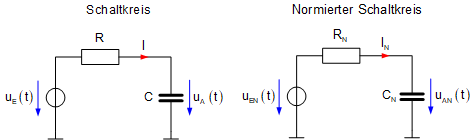
\includegraphics[width=0.7\textwidth]{Kapitel1/Bilder/image27}}
  \caption{Beispiel RC-Netzwerk, normierte und nicht normierte Darstellung }
  \label{fig:RCNETZWERK}
\end{figure}



\noindent Die Kapazit\"{a}t hat einen Wert von C = 1 µF und der Widerstand betr\"{a}gt R = 1 k$\Omega$. Das System wird normiert mit den Gr\"{o}{\ss}en
\begin{equation}\label{eq:onehundredeight}
U_{0} =1  \; V
\end{equation}

\begin{equation}\label{eq:onehundrednine}
{I}_{0} \; =1 \;mA
\end{equation}

\begin{equation}\label{eq:onehundredten}
{t}_{0} =1 \; ms
\end{equation}


\noindent Die normierten Bauelemente haben damit die Werte

\begin{equation}\label{eq:onehundredeleven}
R_{N} =\dfrac{R\cdot I_{0} }{U_{0} } =\dfrac{1{\rm \; }k\Omega \cdot 1{\rm \; }mA}{1V} =1
\end{equation}

\noindent und 

\begin{equation}\label{eq:onehundredtwelve}
C_{N} =C\cdot \dfrac{R_{0} }{T_{0} } =1 \; \mu F\cdot \dfrac{1 \; k\Omega }{1 \; ms} =1
\end{equation}


\noindent Das Ersatzschaltbild des normierten Systems ist in Bild \ref{fig:RCNETZWERK} rechts dargestellt.

\bigskip

{\fontfamily{phv}\selectfont
\noindent\textbf{Zusammenfassung Normierung von Signalen}} \smallskip

\noindent Im Folgenden werden Beispiele normiert berechnet, um die Darstellung kompakter zu halten. Nur in Einzelfällen werden die Einheiten zur Herleitung von Zeitkonstanten, Grenzfrequenzen oder anderen charakteristischen Größen mitgeführt. Die Schritte zur Normierung von Signalen sind in Tabelle \ref{tab:twosix} zusammengefasst.

{\fontfamily{phv}\selectfont
\noindent\textbf{}} \smallskip

\medskip
\begin{table}[H]
\setlength{\arrayrulewidth}{.1em}
\caption{Schritte zur Normierung von Signalen}
\setlength{\fboxsep}{0pt}%
\colorbox{lightgray}{%
\arrayrulecolor{white}%
\begin{tabular}{| c | c |}
\hline
\parbox[c][0.28in][c]{3.3in}{\smallskip\centering\textbf{\fontfamily{phv}\selectfont{Normierung}}} & \parbox[c][0.28in][c]{3.3in}{\smallskip\centering\textbf{\fontfamily{phv}\selectfont{Mathematische Beschreibung}}}\\ \hline

\parbox[c][0.64in][c]{3.3in}{\centering{\fontfamily{phv}\selectfont{Amplitudennormierung}}} & 
\parbox[c][0.64in][c]{3.3in}{\centering{$U_{N} =\dfrac{U}{U_{0} } $}}\\ \hline

\parbox[c][0.64in][c]{3.3in}{\centering{\fontfamily{phv}\selectfont{Zeitnormierung}}} & \parbox[c][0.64in][c]{3.3in}{\centering{$t_{N} =\dfrac{t}{T_{0} } $}}\\
\end{tabular}%
}
\label{tab:twosix}
\end{table}

\bigskip

\noindent In der Regelungstechnik wird statt der hier dargestellten Normierung von Signalen eine Skalierung vorgenommen. Bei der Skalierung werden die Amplituden der Signale geeignet normiert, eine Zeitnormierung findet nicht statt.

\clearpage



\subsection{ Literatur}


\subsubsection{ Literaturstellen zur mathematischen Darstellung}

\begin{tabular}{|p{0.6in}|p{5.7in}|} \hline 
[Papu11] & Papula, Lothar: Mathematik f\"{u}r Ingenieure und Naturwissenschaftler Band 1 - 3, Springer Fachmedien Wiesbaden, 2011 \\ \hline 
[Bron79] & Bronstein, Ilja: Taschenbuch der Mathematik, Wissenschaftlicher Verlag Harri Deutsch, Frankfurt am Main, 2008 \\ \hline 
\end{tabular}


\subsubsection{ Weiterf\"{u}hrende Literatur}

\begin{tabular}{|p{0.6in}|p{5.7in}|} \hline 
[Saue12] & R. Sauer, I. Szabo (Hrsg.): Mathematische Hilfsmittel des IngenieursSpringer-Verlag, 2012 \\ \hline 
[Gelf67] & Gelfand, Israel: Verallgemeinerte Funktionen (Distributionen): Verallgemeinerte Funktionen und das Rechnen mit IhnenVEB Deutscher Verlag der Wissenschaften, Berlin (Ost), 1967. \\ \hline 
[Foel11] & F\"{o}llinger, Otto: Laplace-, Fourier- und z-Transformation. 10., \"{u}berarbeitete AuflageVDE Verlag GmbH, Berlin, Offenbach 2011 \\ \hline 
[Giro05] & Girod, Bernd: Einf\"{u}hrung in die Systemtheorie. 3. AuflageB.G. Teubner Stuttgart, 2005 \\ \hline 
\end{tabular}

\clearpage

\section{Zeitdiskrete Signale}
\noindent Zeitkontinuierliche Signale können mithilfe der Laplace-Transformation in einen sogenannten Laplace-
Bereich transformiert werden. Im Laplace-Bereich lassen sich lineare Differentialgleichungen mit konstanten Koeffizienten vergleichsweise einfach und anschaulich lösen. Rechenregeln der Laplace- Transformation erlauben eine vergleichsweise einfache Behandlung der Anfangsbedingungen. Darüber hinaus eignet sich der Laplace-Bereich zur Charakterisierung von linearen, zeitinvarianten Systemen mit sogenannten Übertragungsfunktionen.\newline

\noindent In diesem Kapitel wird die Laplace-Transformation vorgestellt. Nach der Definition der Laplace-Transformation werden einige Korrespondenzen über die Definitionsgleichung bestimmt. Die eher aufwendige Bestimmung von Korrespondenzen über die Definitionsgleichung kann vermieden werden, wenn die vorliegende Funktion auf Funktionen mit bekannten Korrespondenzen zurückgeführt werden kann. Die dazu notwendigen Rechenregeln werden hergeleitet und der Nutzen an Beispielen demonstriert.\newline

\noindent Anhand eines einfachen Beispiels wird die Bedeutung der Laplace-Transformation für die Lösung von
Differentialgleichungen aufgezeigt. Dabei wird motiviert, warum die Rücktransformation vom Laplace- Bereich in den Zeitbereich erforderlich ist. Die Rücktransformation vom Laplace-Bereich in den Zeitbereich kann grundsätzlich über ein Umkehrintegral erfolgen. Da dieser Weg aufwendig ist und Kenntnisse in der Funktionentheorie voraussetzt, wird er in der Praxis vermieden. Die bei technischen
Anwendungen entstehenden Laplace-Transformierten sind typischerweise gebrochen rationale Funktionen. Sie können in Partialbrüche zerlegt werden, die sich mithilfe der angesprochenen Rechenregeln und einiger Korrespondenzen in den Zeitbereich transformieren lassen.\newline

\noindent Die computerunterstützte Berechnung von Laplace-Transformierten wird anhand des Programms MATLAB beschrieben. Nach der Zusammenstellung der für die analytische Berechnung wesentlichen Befehle werden einige Beispiele und Beweise mithilfe der \textit{Symbolic Math Toolbox} berechnet.

\subsection{Grundlagen der Laplace-Transformation}

\subsubsection{Definitionsgleichung der Laplace-Transformation}\label{threeoneone}

\noindent Für kausale Signale ist die einseitige Laplace-Transformation definiert als

\begin{equation}\label{eq:fourone}
X(s) = \int\limits _{0}^{\infty} x(t) \cdot e^{-s\cdot t} dt
\end{equation}

\noindent Dabei ist s eine komplexe Zahl mit Realteil und Imaginärteil. Das Integral startet dabei an der Stelle t = 0-. Damit schließt das Laplace-Integral in Gleichung (\ref{eq:fourone}) Singularitäten an der Stelle t = 0 mit ein.
Es wird sich zeigen, dass daraus ein Formalismus entsteht, mit dem Übergangsbedingungen elegant bestimmt werden können. Die Transformation wird mit einem großen $L$ symbolisiert.

\begin{equation}\label{eq:fourtwo}
L\left\{x\left(t\right)\right\}=X\left(s\right)=\int\limits _{0_{-} }^{\infty }x\left(t\right)\cdot e^{-s\cdot t} {\rm \; } dt
\end{equation}

\noindent Ein Paar aus Zeitfunktion x(t) und Laplace-Transformierter X(s) wird auch als Korrespondenz bezeichnet. Korrespondenzen werden in der Literatur mit einem halb ausgef\"{u}llten Hantelzeichen dargestellt. Die nicht ausgef\"{u}llte Seite repr\"{a}sentiert dabei den Zeitbereich, die ausgef\"{u}llte Seite den transformierten Bereich.

\begin{equation}\label{eq:fourthree}
x\left(t\right)\circ -\bullet X\left(s\right)
\end{equation}


\noindent Die Laplace-Transformation bildet demnach Zeitfunktionen x(t) auf ihre Laplace-Transformierte X(s) ab. Die Variable s ist eine komplexe Variable. Die zugehörige komplexe Ebene wird auch als s-Ebene bezeichnet. Eine wichtige Eigenschaft der Laplace-Transformation besteht darin, dass der Differentiation und Integration im Zeitbereich einfache algebraische Operationen im Laplace-Bereich entsprechen. Au{\ss}erdem geht eine Faltung im Zeitbereich in eine Multiplikation im Laplace-Bereich \"{u}ber. Diese und andere Eigenschaften werden in Abschnitt 4.2 hergeleitet.

\subsubsection{Laplace-Transformation grundlegender Signale}
\noindent Zur Einführung werden die Laplace-Transformierten von einigen kausalen Funktionen über die Definitionsgleichung der Laplace-Transformation berechnet. Dabei ist zu berücksichtigen, dass im Rahmen dieser Buchreihe die einseitige Laplace-Transformation durchgeführt wird, die nur für kausale Signale definiert ist.\medskip

{\fontfamily{phv}\selectfont
\noindent\textbf{Kausale Rechteckfunktion}}\smallskip

\noindent Eine Rechteckfunktion mit der Gleichung

\begin{equation}\label{eq:fourfour}
x\left(t\right)=\sigma \left(t\right)-\sigma \left(t-t_{0} \right)
\end{equation}

\noindent soll in den Laplace-Bereich transformiert werden. Das Signal ist in Bild \ref{fig:LaplaceSignaleRechteck} dargestellt.

\begin{figure}[H]
  \centerline{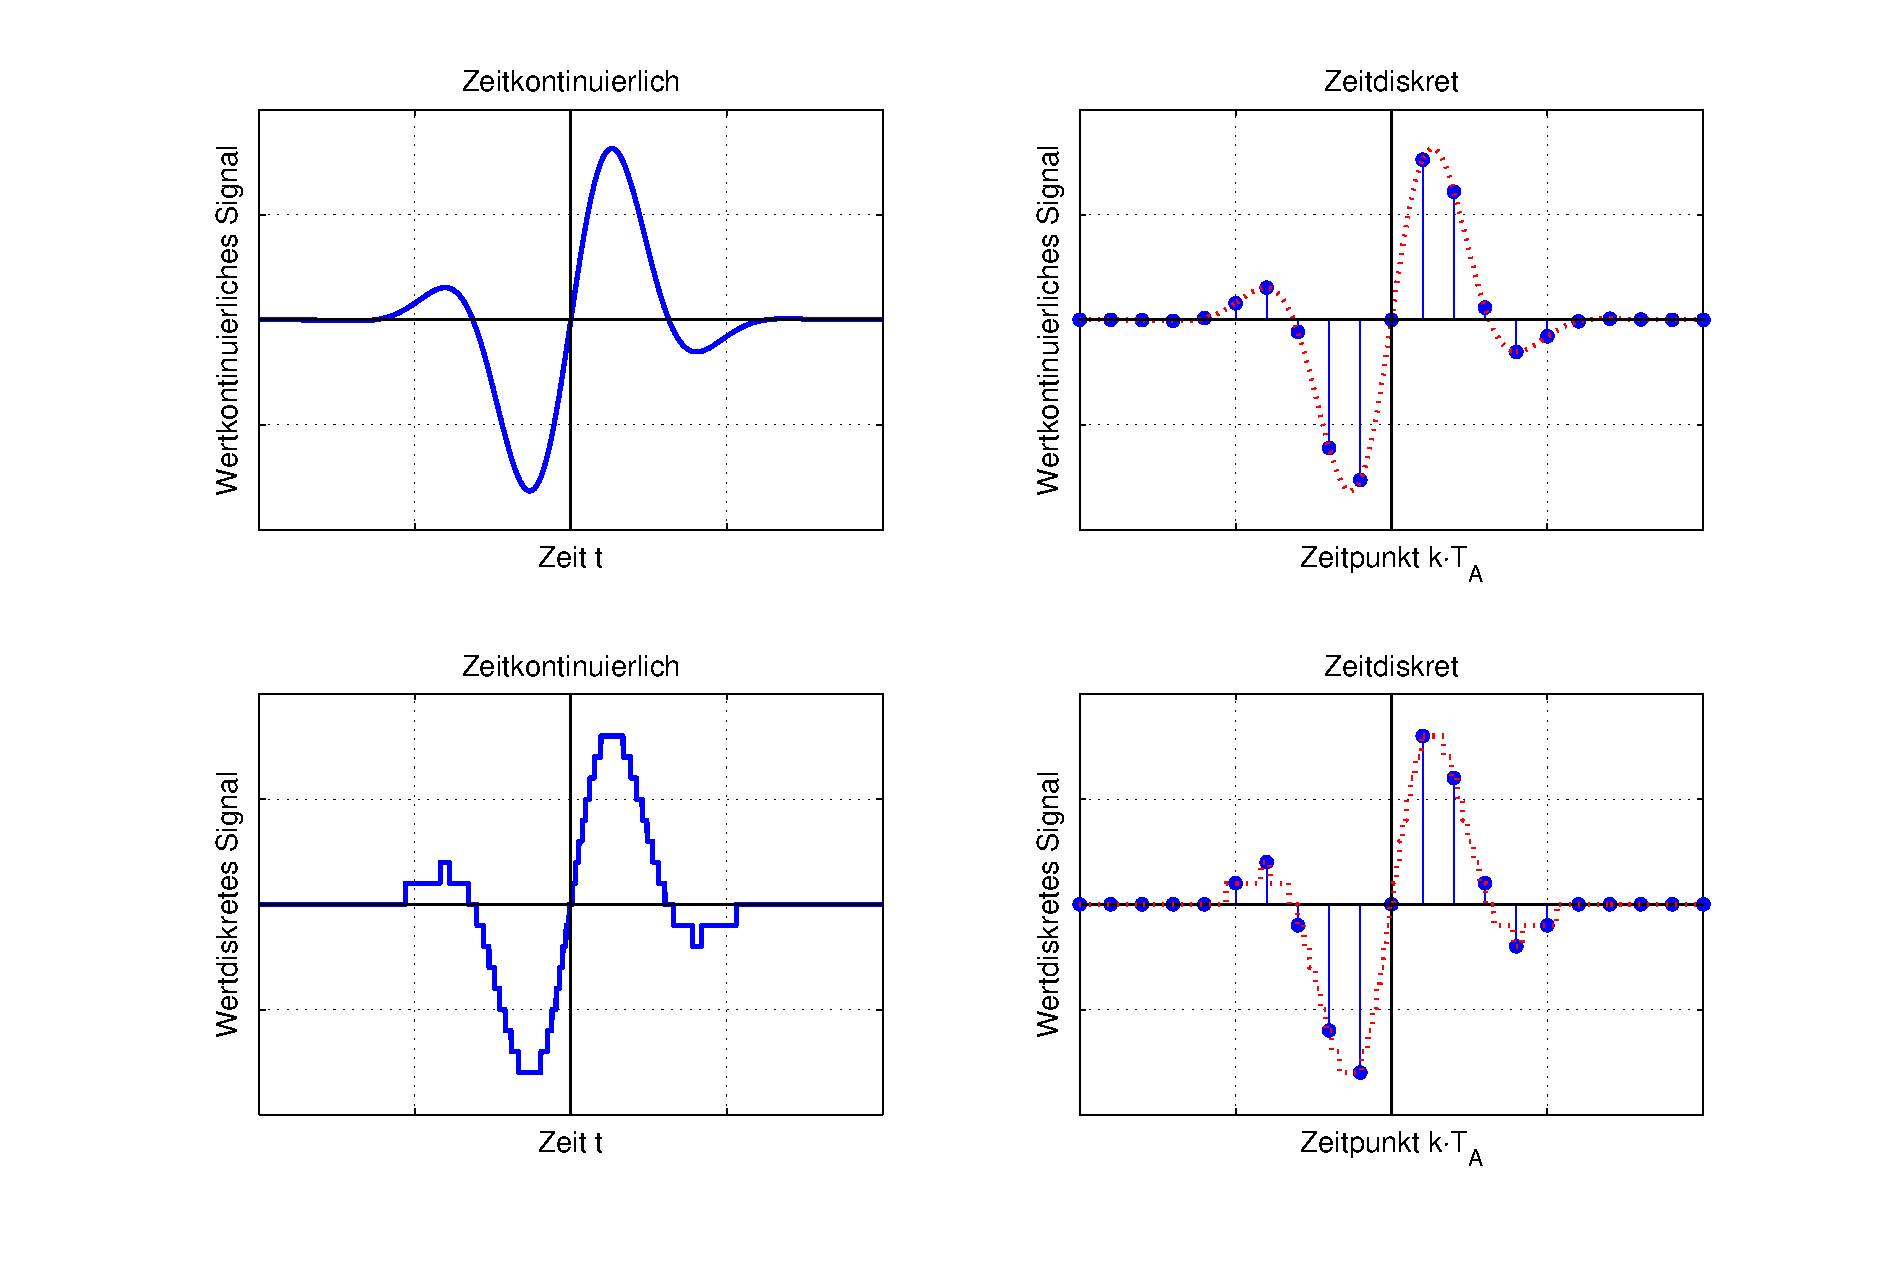
\includegraphics[width=0.5\textwidth]{Kapitel3/Bilder/image1}}
  \caption{Kausale Rechteckfunktion x(t)}
  \label{fig:LaplaceSignaleRechteck}
\end{figure}

\noindent Einsetzen der Zeitfunktion x(t) in die Definitionsgleichung führt zu

\begin{equation}\label{eq:fourfive}
X\left(s\right)=\int\limits _{0_{-} }^{\infty }x\left(t\right)\cdot e^{-s\cdot t} {\rm \; } dt=\int\limits _{0_{-} }^{\infty }\left(\sigma \left(t\right)-\sigma \left(t-t_{0} \right)\right)\cdot e^{-s\cdot t} {\rm \; } dt
\end{equation}

\noindent Die kausale Rechteckfunktion ist nur in dem Bereich von 0${}_{-}$ bis t${}_{0}$ von null verschieden. Damit muss auch die Integration nur in diesem Bereich durchgef\"{u}hrt werden. In dem Bereich ist die Funktion x(t) konstant gleich 1. Damit kann das Integral umgeformt werden zu

\begin{equation}\label{eq:foursix}
X\left(s\right)=\int\limits _{0_{-} }^{\infty }\left(\sigma \left(t\right)-\sigma \left(t-t_{0} \right)\right)\cdot e^{-s\cdot t} {\rm \; } dt=\int\limits _{0_{-} }^{t_{0} }1\cdot e^{-s\cdot t} {\rm \; } dt
\end{equation}

\noindent Mit der Stammfunktion der Exponentialfunktion

\begin{equation}\label{eq:fourseven}
\int\limits e^{a\cdot t} {\rm \; dt} =\frac{1}{a} \cdot e^{a\cdot t}
\end{equation}

\noindent und durch Einsetzen der Integrationsgrenzen ergibt sich die Laplace-Transformierte

\begin{equation}\label{eq:foureight}
X\left(s\right)=\int\limits _{0_{-} }^{t_{0} }1\cdot e^{-s\cdot t} {\rm \; } dt=\left. -\frac{1}{s} \cdot e^{-s\cdot t} \right|_{0_{-} }^{t_{0} } =-\frac{1}{s} \cdot e^{-s\cdot t_{0} } +\frac{1}{s} \cdot e^{-s\cdot 0_{-} } =\frac{1}{s} \cdot \left(1-e^{-s\cdot t_{0} } \right)
\end{equation}
\medskip

{\fontfamily{phv}\selectfont
\noindent\textbf{Impulsfunktion}}\smallskip

\noindent Als weiteres Beispiel werden die Laplace-Transformierten einer Impulsfunktion x$_{1}$(t) und einer verschobenen Impulsfunktion x$_{2}$(t) berechnet. 

\begin{equation}\label{eq:fournine}
x_{1} \left(t\right)=\delta \left(t\right)
\end{equation}

\begin{equation}\label{eq:fourten}
x_{2} \left(t\right)=\delta \left(t-t_{0} \right)
\end{equation}

\noindent Die beiden Signale sind in Bild \ref{fig:LaplaceSignaleImpuls} dargestellt.

\begin{figure}[H]
  \centerline{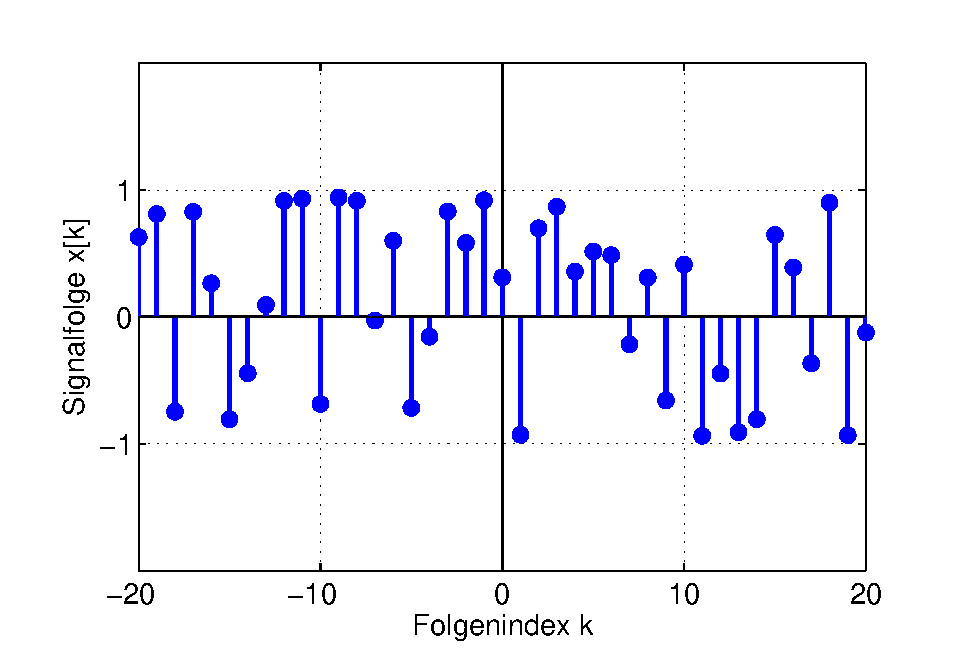
\includegraphics[width=1\textwidth]{Kapitel3/Bilder/image2}}
  \caption{Impulsfunktion x$_{1}$(t) und verschobene Impulsfunktion x$_{2}$(t)}
  \label{fig:LaplaceSignaleImpuls}
\end{figure}

\noindent Einsetzen der Impulsfunktion in die Definitionsgleichung f\"{u}hrt mit der Ausblendeigenschaft der Impulsfunktion zu

\begin{equation}\label{eq:foureleven}
X_{1} \left(s\right)=\int\limits _{0_{-} }^{\infty }\delta \left(t\right)\cdot e^{-s\cdot t} {\rm \; } dt=e^{-s\cdot 0} \cdot \int\limits _{0_{-} }^{\infty }\delta \left(t\right){\rm \; } dt=1\cdot \int\limits _{0_{-} }^{\infty }\delta \left(t\right){\rm \; } dt=1
\end{equation}

\noindent Analog ergibt sich f\"{u}r den verschobenen Impuls die Laplace-Transformierte 

\begin{equation}\label{eq:fourtwelve}
X_{2} \left(s\right)=\int _{0_{-} }^{\infty }\delta \left(t-t_{0} \right)\cdot e^{-s\cdot t} {\rm \; } dt=e^{-s\cdot t_{0} } \cdot \int _{0_{-} }^{\infty }\delta \left(t-t_{0} \right){\rm \; } dt=e^{-s\cdot t_{0} }
\end{equation}

\noindent Die Impulsfunktion $\delta$(t) besitzt die Laplace-Transformierte X(s) = 1. Eine Verschiebung des Impulses um t$_{0}$ nach rechts führt zu der Laplace-Transformierten e$^{-s\cdot t_{0}}$. In Abschnitt 4.2 wird sich zeigen, dass eine Verschiebung der Zeitfunktion um t$_{0}$ nach rechts immer zu einer Multiplikation mit dem Faktor e$^{-s\cdot t_{0}}$ führt.\bigskip

{\fontfamily{phv}\selectfont
\noindent\textbf{Sprungfunktion}}\smallskip

\noindent Die Sprungfunktion $\sigma$(t) springt zum Zeitpunkt t = 0 von null auf den Wert eins. Sie ist in Bild \ref{fig:LaplaceSignaleSprung} dargestellt.

\begin{figure}[H]
  \centerline{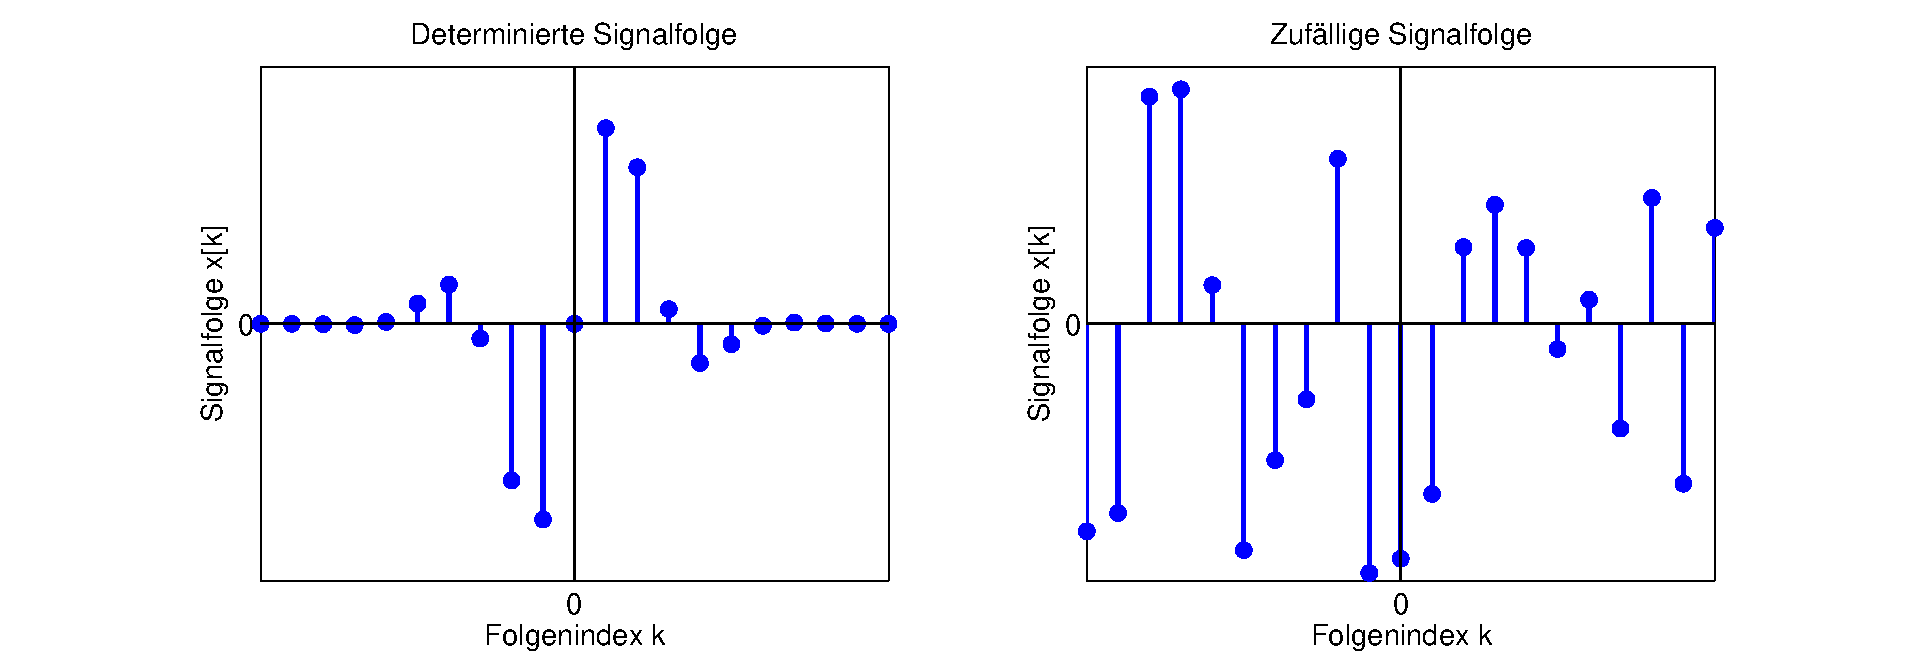
\includegraphics[width=0.5\textwidth]{Kapitel3/Bilder/image3}}
  \caption{Sprungfunktion $\sigma$}
  \label{fig:LaplaceSignaleSprung}
\end{figure}

\begin{equation}\label{eq:fourthirteen}
X\left(s\right)=\int\limits _{0_{-} }^{\infty }\sigma \left(t\right)\cdot e^{-s\cdot t} \;dt=\int\limits _{0_{-} }^{\infty }1\cdot e^{-s\cdot t} \;dt=\int\limits _{0_{-} }^{\infty }e^{-s\cdot t}\; dt
\end{equation}

\noindent Da die Sprungfunktion zeitlich nicht begrenzt ist, weist das Integral einen unendlich langen Integrationsbereich auf. Derartige Integrale werden uneigentliche Integrale genannt. Bilden der Stammfunktion und Einsetzen der Integrationsgrenzen führen zu dem Ausdruck

\begin{equation}\label{eq:fourfourteen}
X\left(s\right)=\left. -\frac{1}{s} \cdot e^{-s\cdot t} \right|_{0_{-} }^{\infty } =-\lim \limits_{t\to \infty } \frac{1}{s} \cdot e^{-s\cdot t} +\frac{1}{s} \cdot e^{-s\cdot 0_{-} } =\frac{1}{s} \cdot \left(1-\lim \limits_{t\to \infty } e^{-s\cdot t} \right)
\end{equation}

\noindent Dabei ist die Zahl s eine komplexe Zahl s = $\delta$ + j$\cdot\omega$. Der Grenzwert existiert nur, wenn der Realteil $\delta$ der komplexen Zahl s positiv ist. In diesem Fall gilt

\begin{equation}\label{eq:fourfifteen}
X\left(s\right)=\frac{1}{s} \cdot \left(1-\lim\limits_{t\to \infty} e^{-s\cdot t} \right)=\frac{1}{s} \cdot \left(1-\lim\limits_{t\to \infty } e^{-\left(\delta +j\cdot \omega \right)\cdot t} \right)=\frac{1}{s} \cdot \left(1-\lim\limits_{t\to \infty } e^{-\delta \cdot t} \cdot e^{-j\cdot \omega \cdot t} \right)=\frac{1}{s} \cdot \left(1-0\right)=\frac{1}{s}
\end{equation}

\noindent Die Sprungfunktion x(t) = $\sigma$(t) hat demnach für den Bereich der s-Ebene mit $\delta$ $\mathrm{>}$ 0 die Laplace-Transformierte X(s) = 1/s. In dem Bereich der s-Ebene mit $\delta$ $\leq$ 0 besitzt die Sprungfunktion keine Laplace-Transformierte, da das Laplace-Integral nicht konvergiert.\medskip

\noindent Zu der Laplace-Transformierten muss demnach immer ein Konvergenzbereich angegeben werden. In den beiden ersten Beispielen ist der Konvergenzbereich unendlich gro{\ss}. Bei der Sprungfunktion liegt der Konvergenzbereich in der positiven Halbebene. Auf die Frage der Konvergenz des Laplace-Integrals wird in Abschnitt 4.1.3 genauer eingegangen.\bigskip

{\fontfamily{phv}\selectfont
\noindent\textbf{Konstanten und kausale Konstanten}}\smallskip

\noindent Die Laplace-Transformierte einer Konstanten x(t) = k ergibt sich analog zu der Berechnung der Laplace-Transformierten der Sprungfunktion zu

\begin{equation}\label{eq:foursixteen}
X\left(s\right)=\int _{0_{-} }^{\infty }k\cdot e^{-s\cdot t} \; dt=k\cdot \int _{0_{-} }^{\infty }e^{-s\cdot t} \; dt=\frac{k}{s}
\end{equation}

\noindent Die Laplace-Transformierten einer Konstante k und einer mit dem Faktor k multiplizierten Sprungfunktion k$\cdot\sigma$(t) unterscheiden sich weder im Ergebnis noch im Konvergenzbereich. Ursache ist die einseitige Laplace-Transformation mit der Definitionsgleichung

\begin{equation}\label{eq:fourseventeen}
X\left(s\right)=\int _{0_{-} }^{\infty }x\left(t\right)\cdot e^{-s\cdot t} \; dt
\end{equation}

\noindent Die Integration beginnt zum Zeitpunkt t = 0$_{-}$, sodass das Verhalten der Funktion für t $\mathrm{<}$ 0 unberücksichtigt bleibt. Da sich Konstanten und Sprungfunktionen aber nur in diesem Bereich unterscheiden, ist ihre Laplace-Transformierte identisch. Bild \ref{fig:LaplaceSignaleKausaleKonstant} verdeutlicht diesen Zusammenhang grafisch.

\begin{figure}[H]
  \centerline{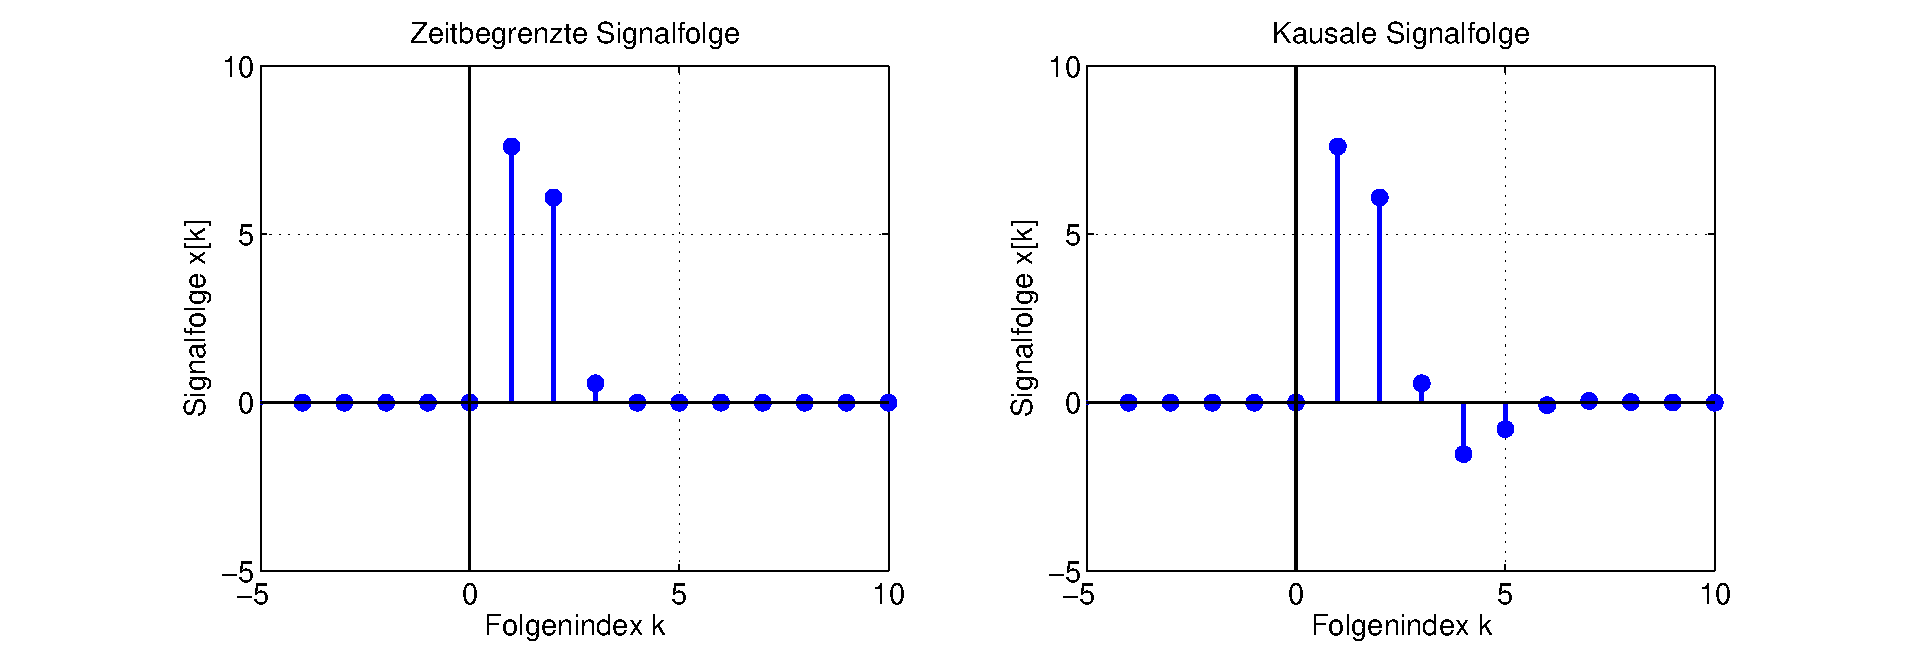
\includegraphics[width=1\textwidth]{Kapitel3/Bilder/image4}}
  \caption{Grafischer Vergleich von kausaler Konstante k$\sigma$(t) und Konstante k}
  \label{fig:LaplaceSignaleKausaleKonstant}
\end{figure}

\noindent Konstanten werden im Zusammenhang mit der Laplace-Transformation auch als kausale Konstanten bezeichnet, also als Konstanten, die erst für t $\geq$ 0 von null verschieden sind.\bigskip

{\fontfamily{phv}\selectfont
\noindent\textbf{Kausale Exponentialfunktion}}\smallskip

\noindent Die kausale Exponentialfunktion ist für t $\mathrm{<}$ 0 null. Zum Zeitpunkt t = 0 springt sie auf den Wert eins. Je nach Koeffizienten $\delta$ steigt die Exponentialfunktion an, bleibt konstant oder fällt ab. 

\begin{equation}\label{eq:foureighteen}
x\left(t\right)=e^{\delta \cdot t} \cdot \sigma \left(t\right) 
\end{equation}

\noindent Bild \ref{fig:KomplexExponentialfunktion} verdeutlicht die Abhängigkeit des Signalverlaufs von dem Koeffizienten $\delta$.

\begin{figure}[H]
  \centerline{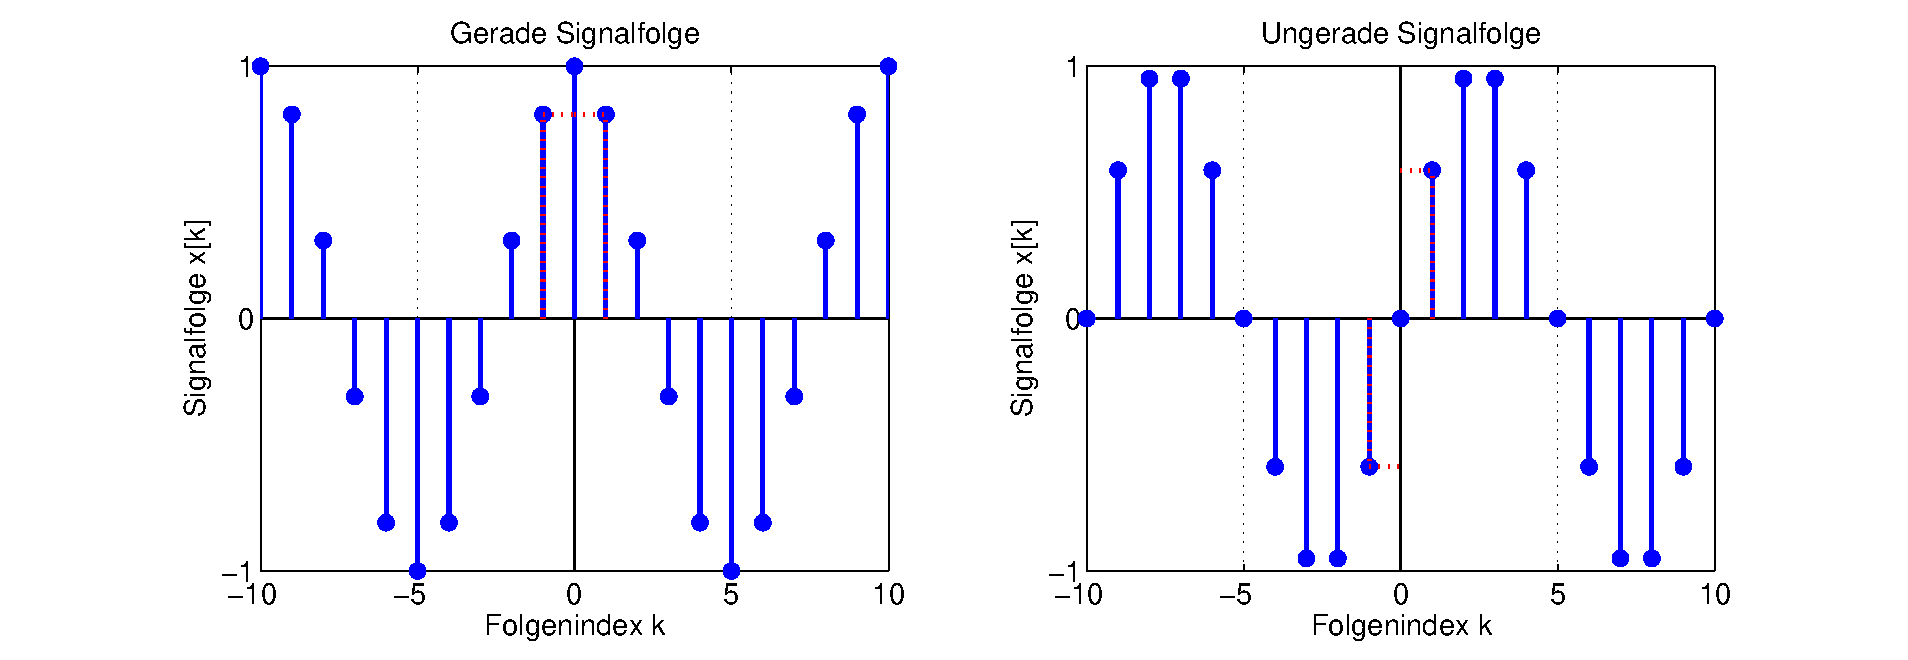
\includegraphics[width=0.5\textwidth]{Kapitel3/Bilder/image5}}
  \caption{Kausale Exponentialfunktion mit unterschiedlichen Koeffizienten $\sigma$ = - 1, 0 und 1}
  \label{fig:LaplaceSignaleExponentialfunktion}
\end{figure}

\noindent Wird die kausale Exponentialfunktion in die Definitionsgleichung für die Laplace-Transformation
eingesetzt, ergibt sich das Integral

\begin{equation}\label{eq:fournineteen}
X\left(s\right)=\int\limits _{0_{-} }^{\infty }e^{\delta \cdot t} \cdot \sigma \left(t\right)\cdot e^{-s\cdot t}\; dt=\int\limits _{0_{-} }^{\infty }e^{\left(\delta -s\right)\cdot t} \;dt 
\end{equation}

\noindent Wieder handelt es sich um ein uneigentliches Integral. Dasselbe Vorgehen wie bei der Sprungfunktion führt zu 

\begin{equation}\label{eq:fourtwenty}
X\left(s\right)=\left. \frac{1}{\delta -s} \cdot e^{\left(\delta -s\right)\cdot t} \right|_{0_{-} }^{\infty } =\lim \limits_{t\to \infty }  \frac{1}{\delta -s} \cdot e^{\left(\delta -s\right)\cdot t} -\frac{1}{\delta -s} \cdot e^{\left(\delta -s\right)\cdot 0_{-} } =\frac{1}{s-\delta } \cdot \left(1-\lim \limits_{t\to \infty } e^{-\left(s-\delta \right)\cdot t} \right)
\end{equation}

\noindent Der Grenzwert existiert nur, wenn Re(s - $\delta$) $\mathrm{>}$ 0 ist. In dem Fall gilt

\begin{equation}\label{eq:fourtwentyone}
X\left(s\right)=\frac{1}{s-\delta } \cdot \left(1-\lim\limits_{t\to \infty } e^{-\left(s-\delta \right)\cdot t} \right)=\frac{1}{s-\delta } 
\end{equation}

\noindent Die kausale Exponentialfunktion hat demnach f\"{u}r den Bereich der s-Ebene mit Re(s - $\delta$) $\mathrm{>}$ 0 die Laplace-Transformierte X(s) = 1/(s - $\delta$). In dem \"{u}brigen Bereich der s-Ebene besitzt die kausale Exponentialfunktion keine Laplace-Transformierte, da das Laplace-Integral nicht konvergiert. 

\subsubsection{Existenz der Laplace-Transformation}

\noindent Die Laplace-Transformation beruht auf der Auswertung des Laplace-Integrals.

\begin{equation}\label{eq:fourtwentytwo}
X\left(s\right)=\int\limits _{0_{-} }^{\infty }x\left(t\right)\cdot e^{-s\cdot t} \; dt
\end{equation}

\noindent Es ist ein uneigentliches Integral, das nur definiert ist, wenn das Integral konvergiert. Diese Bedingung ist erfüllt, wenn x(t) stückweise stetig ist und wenn {\textbar}x(t){\textbar} für t $\rightarrow$ $\infty$ nicht schneller als eine Exponentialfunktion wächst. In dem Fall kann die Funktion x(t) abgeschätzt werden mit 

\begin{equation}\label{eq:fourtwentythree}
\left|x\left(t\right)\right|\le k\cdot e^{\delta \cdot t}
\end{equation}

\noindent Für Re(s) $\mathrm{>}$ $\delta$ ist das zugehörige Laplace-Integral absolut konvergent, und die Laplace-Transformierte existiert. Dies kann durch Einsetzen in das Laplace-Integral verdeutlicht werden. Mit 

\begin{equation}\label{eq:fourtwentyfour}
x\left(t\right)=e^{\delta \cdot t} \cdot \sigma \left(t\right)
\end{equation}

\noindent ergibt sich

\begin{equation}\label{eq:fourtwentyfive}
X\left(s\right)=\int\limits _{0_{-} }^{\infty }e^{\delta \cdot t} \cdot \sigma \left(t\right)\cdot e^{-s\cdot t} \; dt= \int\limits _{0_{-} }^{\infty }e^{\left(\delta -s\right)\cdot t} \; dt= \left. \frac{1}{\delta -s} \cdot e^{-\left(s-\delta \right)\cdot t} \right|_{0_{-} }^{\infty } =\lim \limits_{t\to \infty } \frac{1}{\delta -s} \cdot e^{-\left(s-\delta \right)\cdot t} -\frac{1}{\delta -s}
\end{equation}

\noindent Für Re(s - $\delta$) $\mathrm{<}$ 0 strebt die Exponentialfunktion gegen unendlich, das Integral ist demnach nicht konvergent, die Laplace-Transformierte existiert f\"{u}r diesen Bereich der s-Ebene nicht. F\"{u}r Re(s - $\delta$) $\mathrm{>}$ 0 strebt die Exponentialfunktion für t $\rightarrow$ $\infty$ gegen null. Das Integral ist konvergent, und die Laplace-Transformierte existiert. Bild \ref{fig:KonvergenzBereich} zeigt den Konvergenzbereich des Laplace-Integrals in der komplexen Ebene.

\begin{figure}[H]
  \centerline{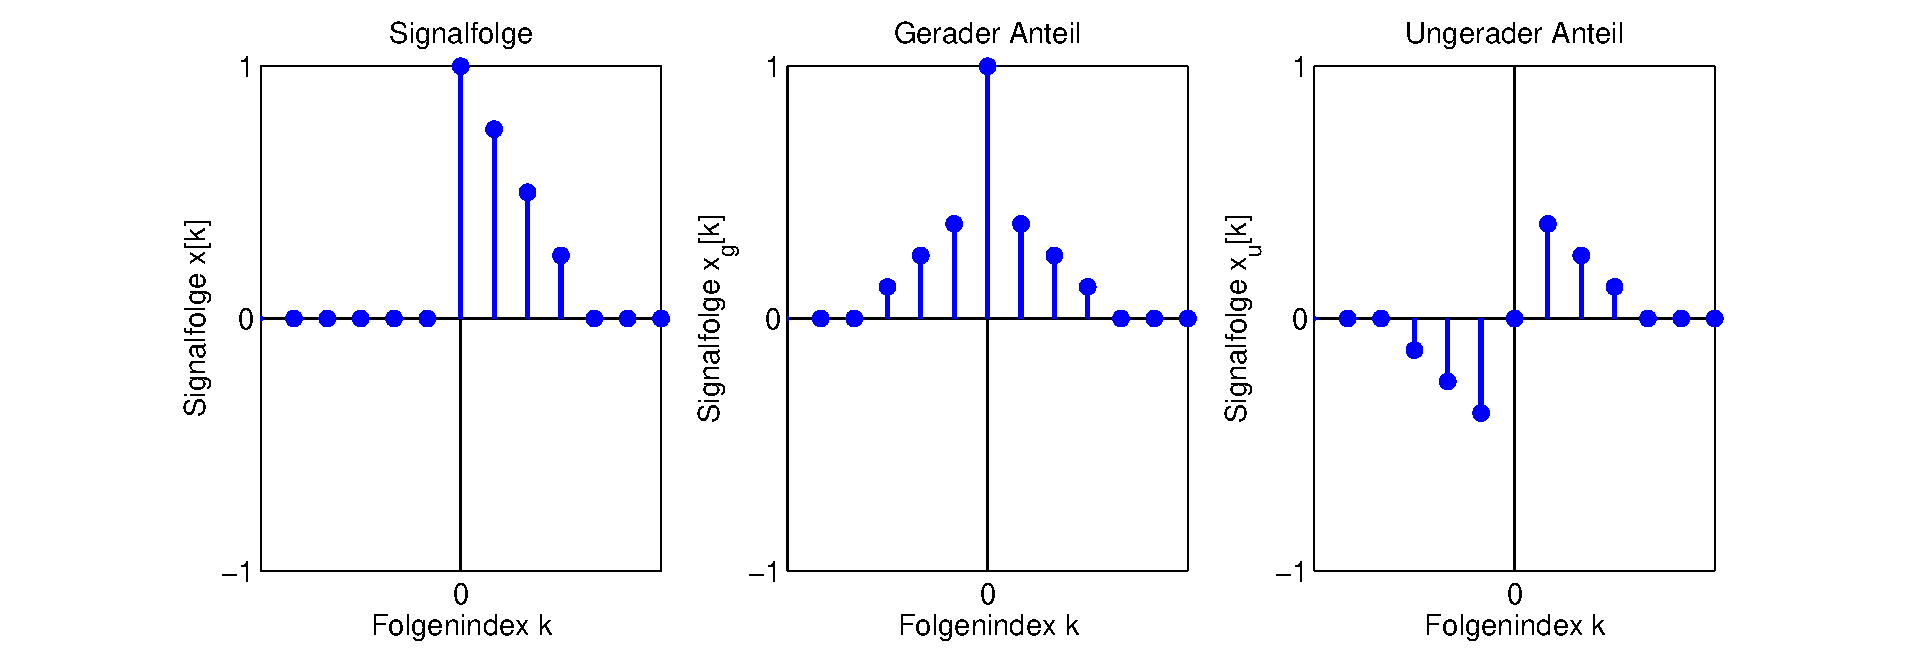
\includegraphics[width=0.4\textwidth]{Kapitel3/Bilder/image6}}
  \caption{Konvergenzbereich für Re(s -$\sigma$) $\mathrm{>}$ 0}
  \label{fig:KonvergenzBereich}
\end{figure}

\noindent Für den grau hinterlegten Bereich der s-Ebene ist das Laplace-Integral konvergent. Allgemein existiert eine Laplace-Transformierte X(s) einer Funktion x(t) also, wenn {\textbar}x(t){\textbar} für t $\rightarrow$ $\infty$ nicht schneller wächst als eine Exponentialfunktion. In den systemtheoretisch interessanten Fällen kann von der Konvergenz des Laplace-Integrals zumindest in einem Teil der s-Ebene ausgegangen werden. Der Konvergenzbereich der Laplace-Transformation ist deshalb für die Berechnung technisch interessanter Fälle von untergeordneter Bedeutung.\medskip

\noindent Bei der sogenannten Fourier-Transformation ist der Konvergenzbereich der Laplace-Transformation wieder wichtig. Es wird sich zeigen, dass sich die Fourier-Transformierte direkt aus der Laplace-Transformierten ergibt, wenn die imagin\"{a}re Achse s = j$\cdot\omega$ im Konvergenzbereich der Laplace-Transformierten liegt.

\clearpage 

\subsubsection{Pollage und kausale Exponentialfunktion}

\noindent Im Abschnitt 4.1.2 wird die Laplace-Transformierte der kausalen Exponentialfunktion

\begin{equation}\label{eq:fourtwentysix}
x\left(t\right)=e^{\lambda \cdot t} \cdot \sigma \left(t\right)
\end{equation}

\noindent berechnet zu

\begin{equation}\label{eq:fourtwentyseven}
X\left(s\right)=\frac{1}{s-\lambda }
\end{equation}

\noindent Aus Gleichung \eqref{eq:fourtwentyseven} kann der zu der Exponentialfunktion zugehörige Pol in der komplexen s-Ebene abgelesen werden.

\begin{equation}\label{eq:fourtwentyeight}
s=\lambda 
\end{equation}

\noindent Die Lage des Poles beziehungsweise der Pole in der s-Ebene kann damit einem Signalverhalten zugeordnet werden, das in Tabelle\ref{tab:fourone} skizziert ist.\medskip

\noindent Kosinusfunktionen mit exponentiell abklingender Amplitude k\"{o}nnen nach den Darstellungen in Abschnitt 2.4.2 als Summe zweier Exponentialfunktionen mit jeweils konjugiert komplexen Koeffizienten $\lambda$ dargestellt werden. 


\begin{equation}\label{eq:fourtwentynine}
\begin{split}
x\left(t\right) & = A\cdot e^{\delta _{0} \cdot t} \cdot \cos \left(\omega _{0} \cdot t\right)\cdot \sigma \left(t\right)=\frac{1}{2} \cdot A\cdot e^{\delta _{0} \cdot t} \cdot \left(e^{j\cdot \omega _{0} \cdot t} +e^{-j\cdot \omega _{0} \cdot t} \right)\cdot \sigma \left(t\right) \\ 
& = \frac{1}{2} \cdot A\cdot \left(e^{\left(\delta _{0} +j\cdot \omega _{0} \right)\cdot t} +e^{\left(\delta _{0} -j\cdot \omega _{0} \right)\cdot t} \right)\cdot \sigma \left(t\right)
\end{split}
\end{equation}

\noindent Jede Exponentialfunktion führt zu einem Pol in der komplexen Ebene, sodass in diesem Fall konjugiert komplexe Polpaare auftreten. Der Realteil $\delta{0}$ der Pole beschreibt das Verhalten der Amplitude, die Imagin\"{a}rteil $\omega _{0}$ repräsentiert die Kreisfrequenz, mit der das Signal schwingt. Die Lage der konjugiert komplexen Polpaare und das entsprechende Signalverhalten sind ebenfalls in Tabelle \ref{tab:fourone} skizziert.\medskip

\noindent Der Zusammenhang von Pollage der Laplace-Transformierten X(s) und dem Einschwingverhalten der zugehörigen Zeitfunktion x(t) ist Grundlage für die Interpretation linearer, zeitinvarianter Systeme im Laplace-Bereich.

\InsertBoxL{0}{\includegraphics[scale=0.5]{code}} 
\textcolor{white}{.}\newline
\noindent Im Online-Portal \textit{Systemtheorie Online} verdeutlicht die Applikation \textit{Komplexe Exponentialfunktion} den Zusammenhang zwischen der Lage des Wertes $\lambda = \delta + j.\omega{}_{0}$ in der komplexen Ebene und dem Verhalten der Schwingung.\newline

\clearpage

\begin{table}[ht]
\setlength{\arrayrulewidth}{.1em}
\caption{Zusammenhang zwischen Pollage der Laplace-Transformierten X(s) in der komplexen Ebene und
Signalverlauf x(t)}
\setlength{\fboxsep}{0pt}%
\colorbox{lightgray}{%
\arrayrulecolor{white}%
\begin{tabular}{| c | c |}
\hline
\parbox[c][0.28in][c]{3.2in}{\smallskip\centering\textbf{\fontfamily{phv}\selectfont{Pollage X(s)}}} & \parbox[c][0.28in][c]{3.2in}{\smallskip\centering\textbf{\fontfamily{phv}\selectfont{Signalverlauf x(t)}}}\\ \hline

\parbox[c][1.6in][c]{3.2in}{\centerline{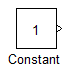
\includegraphics[width=0.3\textwidth]{Kapitel3/Table/image1.png}}} & \parbox[c][1.6in][c]{3.2in}{\centerline{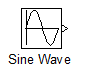
\includegraphics[width=0.3\textwidth]{Kapitel3/Table/image2.png}}}\\ \hline

\parbox[c][1.6in][c]{3.2in}{\centerline{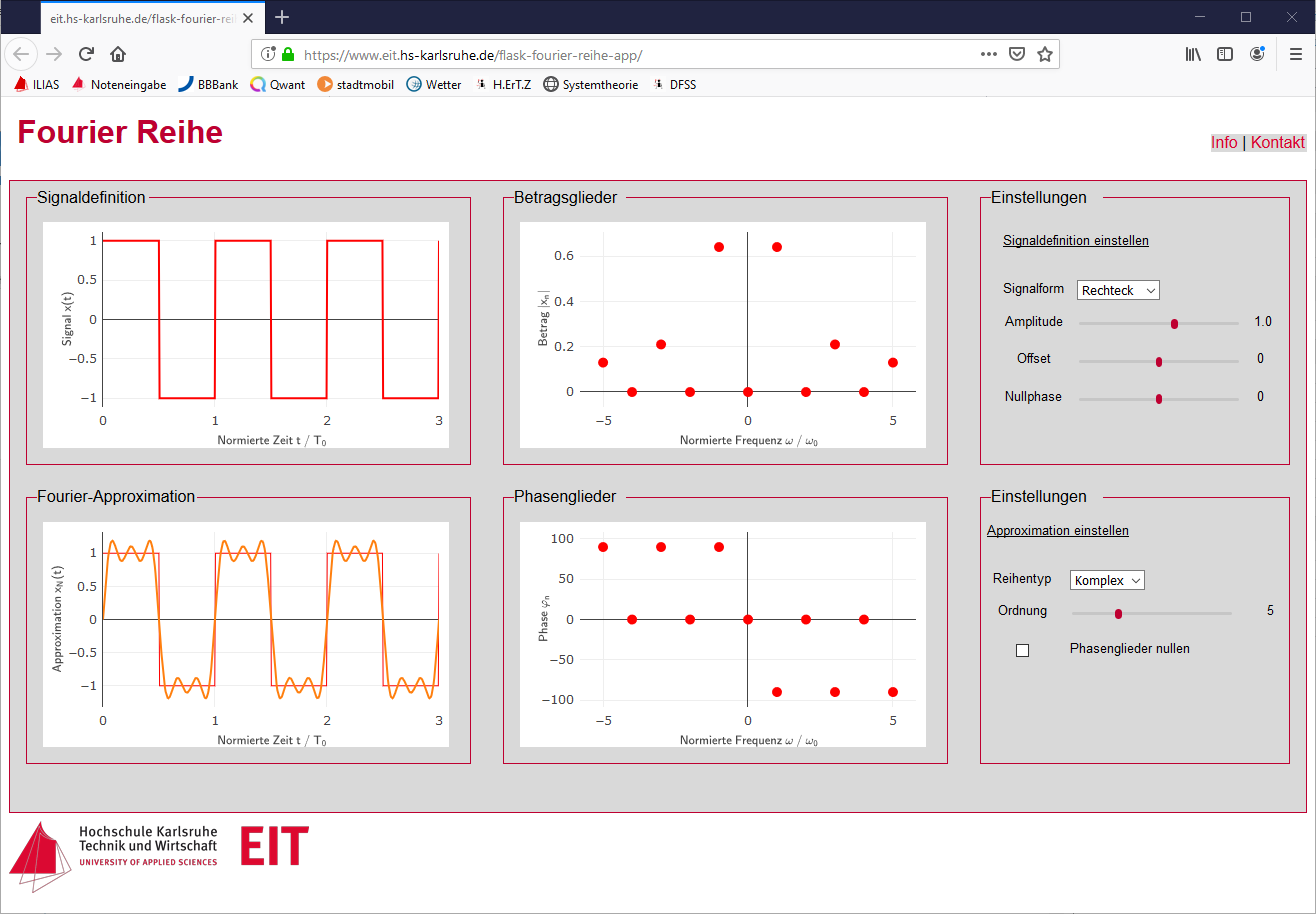
\includegraphics[width=0.3\textwidth]{Kapitel3/Table/image3.png}}} & \parbox[c][1.6in][c]{3.2in}{\centerline{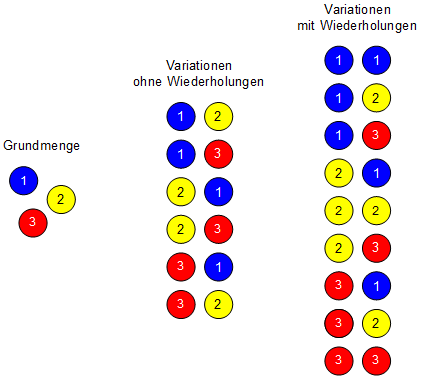
\includegraphics[width=0.3\textwidth]{Kapitel3/Table/image4.png}}}\\ \hline

\parbox[c][1.6in][c]{3.2in}{\centerline{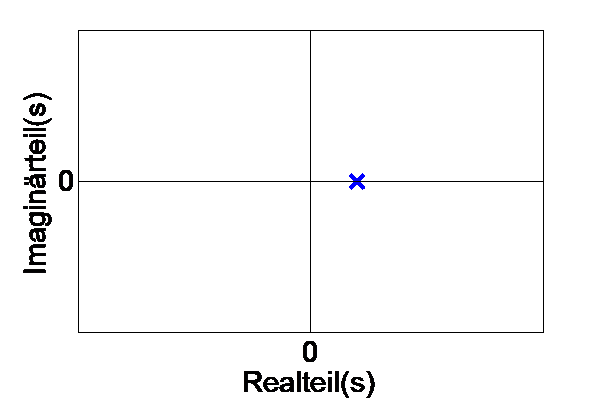
\includegraphics[width=0.3\textwidth]{Kapitel3/Table/image5.png}}} & \parbox[c][1.6in][c]{3.2in}{\centerline{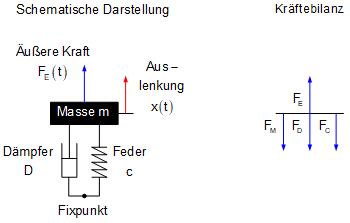
\includegraphics[width=0.3\textwidth]{Kapitel3/Table/image6.png}}}\\ \hline

\parbox[c][1.6in][c]{3.2in}{\centerline{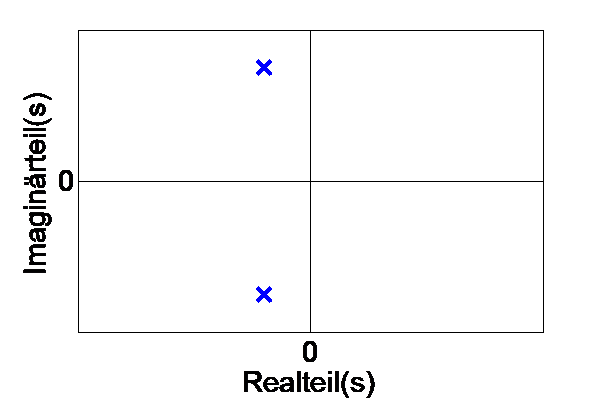
\includegraphics[width=0.3\textwidth]{Kapitel3/Table/image7.png}}} & \parbox[c][1.6in][c]{3.2in}{\centerline{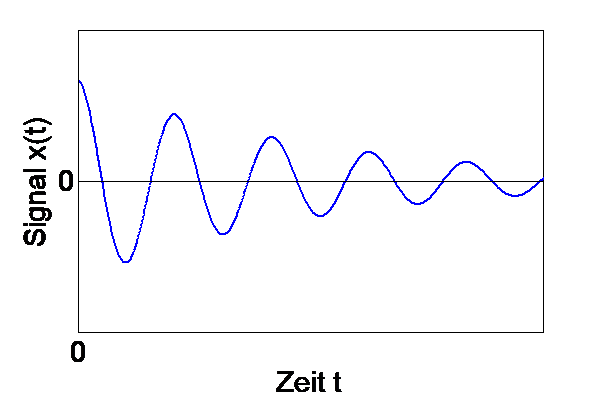
\includegraphics[width=0.3\textwidth]{Kapitel3/Table/image8.png}}}\\ \hline

\parbox[c][1.6in][c]{3.2in}{\centerline{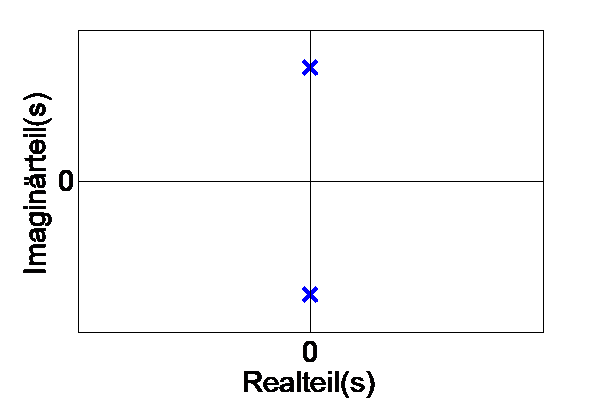
\includegraphics[width=0.3\textwidth]{Kapitel3/Table/image9.png}}} & \parbox[c][1.6in][c]{3.2in}{\centerline{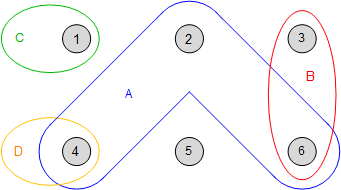
\includegraphics[width=0.3\textwidth]{Kapitel3/Table/image10.png}}}\\ \hline

\parbox[c][1.6in][c]{3.2in}{\centerline{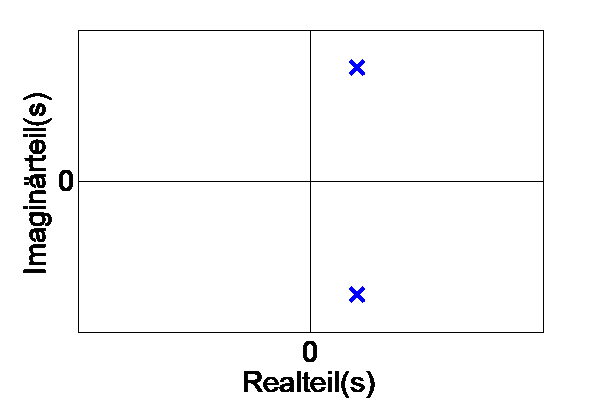
\includegraphics[width=0.3\textwidth]{Kapitel3/Table/image11.png}}} & \parbox[c][1.6in][c]{3.2in}{\centerline{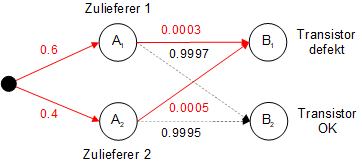
\includegraphics[width=0.3\textwidth]{Kapitel3/Table/image12.png}}}\\ \hline
\end{tabular}%
}
\label{tab:fourone}
\end{table}

\clearpage

\subsection{Rechenregeln der Laplace-Transformation}

\noindent Die Berechnung von Laplace-Transformierten kann über die Auswertung des Laplace-Integrals erfolgen. Dieser Weg ist jedoch oft aufwendig, sodass in der Praxis bereits berechnete Korrespondenzen verwendet werden, um Signale in den Laplace-Bereich zu transformieren. Dazu ist es erforderlich,
Rechenregeln der Laplace-Transformation zu nutzen, um auf standardisierte Ausdrücke zu kommen.
Diese Rechenregeln werden im Folgenden hergeleitet und zusammengefasst. Dabei wird davon ausgegangen, dass die Signale x(t) kausale Signale sind.

\subsubsection{Linearitätsprinzip}

\noindent Die Laplace-Transformation ist eine lineare Transformation. Damit kann eine Linearkombination zweier Funktionen im Laplace-Bereich über dieselbe Linearkombination der jeweiligen Laplace-Transformierten dargestellt werden.

\begin{equation}\label{eq:fourthirty}
L\left\{\nu _{1} \cdot x_{1} \left(t\right)+\nu _{2} \cdot x_{2} \left(t\right)\right\}=\nu _{1} \cdot X_{1} \left(s\right)+\nu _{2} \cdot X_{2} \left(s\right)
\end{equation}

\noindent Der Beweis der Linearität beruht auf der Linearität der Integralrechnung.

\begin{equation}\label{eq:fourthirtyone}
\begin{split}
& L\left\{\nu _{1} \cdot x_{1} \left(t\right)+\nu _{2} \cdot x_{2} \left(t\right)\right\}=\int _{0_{-} }^{\infty }\left(\nu _{1} \cdot x_{1} \left(t\right)+\nu _{2} \cdot x_{2} \left(t\right)\right)\cdot e^{-s\cdot t} {\rm \; } dt \\ 
& =\nu _{1} \cdot \int _{0_{-} }^{\infty }x_{1} \left(t\right)\cdot e^{-s\cdot t} {\rm \; } dt+\nu _{2} \cdot \int _{0_{-} }^{\infty }x_{2} \left(t\right)\cdot e^{-s\cdot t} {\rm \; } dt=\nu _{1} \cdot X_{1} \left(s\right)+\nu _{2} \cdot X_{2} \left(s\right)
\end{split}
\end{equation}\bigskip

\noindent
\colorbox{lightgray}{%
\arrayrulecolor{white}%
\renewcommand\arraystretch{0.6}%
\begin{tabular}{ wl{16.5cm} }
{\fontfamily{phv}\selectfont{Beispiel: Linearität der Laplace-Transformation} }
\end{tabular}%
}\bigskip

\noindent Die Linearitätseigenschaft der Laplace-Transformation kann genutzt werden, um die exponentiell abklingende harmonische Schwingung in den Laplace-Bereich zu transformieren. Sie kann als Summe zweier komplexer Exponentialfunktionen dargestellt werden

\begin{equation}\label{eq:fourthirtytwo}
\begin{split}
x\left(t\right) & = A\cdot e^{\delta \cdot t} \cdot \cos \left(\omega _{0} \cdot t\right)\cdot \sigma \left(t\right)=\frac{1}{2} \cdot A\cdot e^{\delta \cdot t} \cdot \left(e^{j\cdot \omega _{0} \cdot t} +e^{-j\cdot \omega _{0} \cdot t} \right)\cdot \sigma \left(t\right) \\ 
& = {\frac{1}{2} \cdot A\cdot \left(e^{\left(\delta +j\cdot \omega _{0} \right)\cdot t} +e^{\left(\delta -j\cdot \omega _{0} \right)\cdot t} \right)\cdot \sigma \left(t\right)} 
\end{split}
\end{equation}

\noindent Für Exponentialfunktionen ist die Laplace-Transformierte bekannt, sodass die Summe die Laplace-Transformierte

\begin{equation}\label{eq:fourthirtythree}
X\left(s\right)=\frac{1}{2} \cdot A\cdot \left(\frac{1}{s-\left(\delta +j\cdot \omega _{0} \right)} +\frac{1}{s-\left(\delta -j\cdot \omega _{0} \right)} \right)=A\cdot \frac{s-\delta }{\left(s-\delta \right)^{2} +\omega _{0}^{2} } 
\end{equation}

\noindent aufweist. Analog ergibt sich für eine abklingende Sinusfunktion 

\begin{equation}\label{eq:fourthirtyfour}
L\left\{A\cdot e^{\delta \cdot t} \cdot \sin \left(\omega _{0} \cdot t\right)\cdot \sigma \left(t\right)\right\}=A\cdot \frac{\omega _{0} }{\left(s-\delta \right)^{2} +\omega _{0}^{2} }
\end{equation}

\subsubsection{Verschiebungsregel der Zeitfunktion nach rechts, Transport Delay}

\noindent Eine Verschiebung einer Zeitfunktion um t${}_{0}$ nach rechts kann durch x(t - t${}_{0}$) dargestellt werden. Dabei ist t${}_{0}$ eine feste Zahl mit t${}_{0}$ $\mathrm{>}$ 0. F\"{u}r die Funktion im Laplace-Bereich gilt

\begin{equation}\label{eq:fourthirtyfive}
L\left\{x\left(t-t_{0} \right)\right\}=e^{-s\cdot t_{0} } \cdot X\left(s\right)
\end{equation}

\noindent Für den Beweis dieses Verschiebungssatzes wird die Definitionsgleichung der Laplace-Transformation verwendet.

\begin{equation}\label{eq:fourthirtysix}
\begin{split}
L\left\{x\left(t-t_{0} \right)\right\} & = \int\limits _{0_{-} }^{\infty }x\left(t-t_{0} \right)\cdot e^{-s\cdot t}\;dt=\int\limits _{0_{-} }^{\infty }x\left(t-t_{0} \right)\cdot e^{-s\cdot (t-t_{0} )} \cdot e^{-s\cdot t_{0} } \;dt \\ 
& = e^{-s\cdot t_{0} } \cdot \int\limits _{0_{-} }^{\infty }x\left(t-t_{0} \right)\cdot e^{-s\cdot (t-t_{0} )}  \;dt=e^{-s\cdot t_{0} } \cdot \int\limits _{-t_{0} }^{\infty }x\left(t\right)\cdot e^{-s\cdot t}  \;dt \\ 
& = e^{-s\cdot t_{0} } \cdot \int\limits _{-t_{0} }^{0}x\left(t\right)\cdot e^{-s\cdot t} \; dt+e^{-s\cdot t_{0} } \cdot \int\limits _{0_{-} }^{\infty }x\left(t\right)\cdot e^{-s\cdot t}  \;dt
\end{split}
\end{equation}

\noindent Unter der Voraussetzung, dass es sich um ein kausales Signal handelt, ist das erste Integral null, das zweite Integral ist die Laplace-Transformierte X(s) des Zeitsignals x(t). Damit gilt für kausale Signale

\begin{equation}\label{eq:fourthirtyseven}
L\left\{x\left(t-t_{0} \right)\right\}=e^{-s\cdot t_{0} } \cdot X\left(s\right)
\end{equation}

\noindent Der Verschiebung einer kausalen Zeitfunktion um t$_{0}$ nach rechts entspricht eine Multiplikation mit e$^{{\mathrm{-s}\cdot\mathrm{t}}_0}$ im Laplace-Bereich. Eine Verschiebung der Zeitfunktion nach rechts wird bei technischen Anwendungen dazu genutzt, Transportvorg\"{a}nge zu beschreiben. Deshalb hat sich f\"{u}r die Zeitverschiebung der englische Begriff \textit{Transport Delay} durchgesetzt. \bigskip

\noindent
\colorbox{lightgray}{%
\arrayrulecolor{white}%
\renewcommand\arraystretch{0.6}%
\begin{tabular}{ wl{16.5cm} }
{\fontfamily{phv}\selectfont{Beispiel: Verschiebungsregel der Laplace-Transformation}}
\end{tabular}%
}\bigskip

\noindent Die kausale Rechteckfunktion kann durch zwei verschobene Sprungfunktionen dargestellt werden.

\begin{equation}\label{eq:fourthirtyeight}
x\left(t\right)=\sigma \left(t\right)-\sigma \left(t-t_{0} \right)
\end{equation}

\noindent Mit der Verschiebungsregel und der bereits berechneten Korrespondenz der Sprungfunktion

\begin{equation}\label{eq:fourthirtynine}
L\left\{\sigma \left(t\right)\right\}=\frac{1}{s} 
\end{equation}

\noindent ergibt sich die Funktion im Laplace-Bereich

\begin{equation}\label{eq:fourfourty}
X\left(s\right)=\frac{1}{s} -\frac{1}{s} \cdot e^{-s\cdot t_{0} } =\frac{1}{s} \cdot \left(1-e^{-s\cdot t_{0} } \right)
\end{equation}

\noindent Das Ergebnis entspricht dem in Abschnitt 4.1.2 \"{u}ber die Definitionsgleichung der Laplace-Transformation berechneten Ergebnis.

\clearpage

\subsubsection{Modulationsregel}

\noindent Bei der Verschiebungsregel führt eine Verschiebung der Zeitfunktion zu der Multiplikation der Laplace-Transformierten mit einer Exponentialfunktion. Umgekehrt gilt der Zusammenhang

\begin{equation}\label{eq:fourfourtyone}
L\left\{e^{\lambda \cdot t} \cdot x\left(t\right)\right\}=X\left(s-\lambda \right)
\end{equation}

\noindent Dabei ist $\lambda$ eine beliebige komplexe Zahl. Der Beweis beruht wieder auf der Definitionsgleichung des Laplace-Integrals.

\begin{equation}\label{eq:fourfourtytwo}
L\left\{e^{\lambda \cdot t} \cdot x\left(t\right)\right\}=\int\limits _{0_{-} }^{\infty }x\left(t\right)\cdot e^{\lambda \cdot t} \cdot e^{-s\cdot t}\; dt=\int\limits _{0_{-} }^{\infty }x\left(t\right)\cdot e^{-(s-\lambda )\cdot t}\; dt=X\left(s-\lambda \right)
\end{equation}

\noindent Der Multiplikation der Zeitfunktion mit der Exponentialfunktion e$^{\lambda\cdot t}$ entspricht im Laplace-Bereich einer Verschiebung der Funktion um $\lambda$.\bigskip

\noindent
\colorbox{lightgray}{%
\arrayrulecolor{white}%
\renewcommand\arraystretch{0.6}%
\begin{tabular}{ wl{16.5cm} }
{\fontfamily{phv}\selectfont{Beispiel: Modulationsregel der Laplace-Transformation}}
\end{tabular}%
}\bigskip

\noindent Die kausale Sinusfunktion kann mithilfe der Eulerschen Formel dargestellt werden als die Summe von
zwei komplexen Exponentialfunktionen.

\begin{equation}\label{eq:fourfourtythree}
x\left(t\right)=\sin \left(\omega _{0} \cdot t\right)\cdot \sigma \left(t\right)=\frac{1}{2\cdot j} \cdot \left(e^{j\cdot \omega _{0} \cdot t} -e^{-j\cdot \omega _{0} \cdot t} \right)\cdot \sigma \left(t\right)=\frac{1}{2\cdot j} \cdot e^{j\cdot \omega _{0} \cdot t} \cdot \sigma \left(t\right)-\frac{1}{2\cdot j} \cdot e^{-j\cdot \omega _{0} \cdot t} \cdot \sigma \left(t\right)
\end{equation}

\noindent Die Multiplikation der Sprungfunktion mit den Exponentialfunktionen kann als Modulation aufgefasst werden. Mit der Korrespondenz der Sprungfunktion und der Modulationsregel berechnet sich die Korrespondenz der Sinusfunktion zu

\begin{equation}\label{eq:fourfourtyfour}
X\left(s\right)=\frac{1}{2\cdot j} \cdot \frac{1}{s-j\cdot \omega _{0} } -\frac{1}{2\cdot j} \cdot \frac{1}{s+j\cdot \omega _{0} } =\frac{\omega _{0} }{s^{2} +\omega _{0}^{2} }
\end{equation}

\noindent Analog ergibt sich für die Kosinusfunktion

\begin{equation}\label{eq:fourfourtyfive}
L\left\{\cos \left(\omega _{0} \cdot t\right)\cdot \sigma \left(t\right)\right\}=\frac{1}{2} \cdot \frac{1}{s-j\cdot \omega _{0} } +\frac{1}{2} \cdot \frac{1}{s+j\cdot \omega _{0} } =\frac{s}{s^{2} +\omega _{0}^{2} } 
\end{equation}

\subsubsection{Lineare Gewichtung der Zeitfunktion}

\noindent Die Regel zur linearen Gewichtung der Zeitfunktion x(t) ergibt sich durch Ableitung der Laplace-Transformierten X(s) nach der komplexen Variablen s.

\begin{equation}\label{eq:fourfourtysix}
\frac{d}{ds} X\left(s\right)=\frac{d}{ds} \, \, \int\limits _{0_{-} }^{\infty }x\left(t\right)\cdot e^{-s\cdot t} \;dt=\int\limits _{0_{-} }^{\infty }-t\cdot x\left(t\right)\cdot e^{-s\cdot t} \; dt
\end{equation}

\noindent Multiplikation der Gleichung mit - 1 führt zu der Rechenregel der linearen Gewichtung.

\begin{equation}\label{eq:fourfourtyseven}
L\left\{t\cdot x\left(t\right)\right\}=-\frac{dX}{ds} 
\end{equation}\bigskip

\noindent
\colorbox{lightgray}{%
\arrayrulecolor{white}%
\renewcommand\arraystretch{0.6}%
\begin{tabular}{ wl{16.5cm} }
{\fontfamily{phv}\selectfont{Beispiel: Lineare Gewichtung bei der Laplace-Transformation}}
\end{tabular}%
}\bigskip

\noindent Die Laplace-Transformierte der Funktion

\begin{equation}\label{eq:fourfourtyeight}
x\left(t\right)=t\cdot e^{\lambda \cdot t} 
\end{equation}

\noindent kann mit der linearen Gewichtung berechnet werden. Es ergibt sich 

\begin{equation}\label{eq:fourfourtynine}
X\left(s\right)=-\frac{d}{ds} \frac{1}{s-\lambda } =-\frac{d}{ds} \left(s-\lambda \right)^{-1} =\left(s-\lambda \right)^{-2} =\frac{1}{\left(s-\lambda \right)^{2} } 
\end{equation}

\subsubsection{Skalierungsregel}

\noindent Wird die Funktionen x(t) gedehnt oder gestaucht, gilt für die Laplace-Transformierte bei einer reellen Konstante c $\mathrm{>}$ 0

\begin{equation}\label{eq:fourfifty}
L\left\{x\left(c\cdot t\right)\right\}=\frac{1}{c} \cdot X\left(\frac{s}{c} \right)
\end{equation}

\noindent Die Beziehung ergibt sich wieder aus der Integralrechnung.

\begin{equation}\label{eq:fourfiftyone}
L\left\{x\left(c\cdot t\right)\right\}=\int\limits _{0_{-} }^{\infty }x\left(c\cdot t\right)\cdot e^{-s\cdot t} \;  dt=\int\limits _{0_{-} }^{\infty }x\left(c\cdot t\right)\cdot e^{-\frac{s}{c} \cdot c\cdot t} \;  dt
\end{equation}

\noindent Mit der Substitution $\tau$ = c$\cdot$t und d$\tau$/dt = c ergibt die Laplace-Transformierte 

\begin{equation}\label{eq:fourfiftytwo}
L\left\{x\left(c\cdot t\right)\right\}=\int\limits _{0_{-} }^{\infty }x\left(c\cdot t\right)\cdot e^{-\frac{s}{c} \cdot c\cdot t} \; dt=\frac{1}{c} \cdot \int\limits _{0_{-} }^{\infty }x\left(\tau \right)\cdot e^{-\frac{s}{c} \cdot \tau } \; d\tau =\frac{1}{c} \cdot X\left(\frac{s}{c} \right)
\end{equation}

\noindent Analog gilt:

\begin{equation}\label{eq:fourfiftythree}
L\left\{\frac{1}{c} \cdot x\left(\frac{t}{c} \right)\right\}=X\left(c\cdot s\right)
\end{equation}\bigskip

\noindent
\colorbox{lightgray}{%
\arrayrulecolor{white}%
\renewcommand\arraystretch{0.6}%
\begin{tabular}{ wl{16.5cm} }
{\fontfamily{phv}\selectfont{Beispiel: Skalierungsregel der Laplace-Transformation}}
\end{tabular}%
}\bigskip

\noindent Die Rechteckfunktion 

\begin{equation}\label{eq:fourfiftyfour}
x\left(t\right)=\sigma \left(t\right)-\sigma \left(t-t_{0} \right)
\end{equation}

\noindent hat die Laplace-Transformierte 

\begin{equation}\label{eq:fourfiftyfive}
X\left(s\right)=\frac{1}{s} -\frac{1}{s} \cdot e^{-s\cdot t_{0} } =\frac{1}{s} \cdot \left(1-e^{-s\cdot t_{0} } \right)
\end{equation}

\noindent Wird sie um den Faktor 2 gestaucht, 

\begin{equation}\label{eq:fourfiftysix}
y\left(t\right)=x\left(2\cdot t\right)=\sigma \left(2\cdot t\right)-\sigma \left(2\cdot t-t_{0} \right)
\end{equation}

\noindent ergibt sich für die Laplace-Transformierte

\begin{equation}\label{eq:fourfiftyseven}
Y\left(s\right)=\frac{1}{2} \cdot \frac{2}{s} \cdot \left(1-e^{-\frac{s}{2} \cdot t_{0} } \right)=\frac{1}{s} \cdot \left(1-e^{-s\cdot \frac{t_{0} }{2} } \right)
\end{equation}

\noindent Die Gleichung entspricht dem erwarteten Ergebnis, da die Rechteckfunktion bei einer Stauchung um einen Faktor 2 nur noch halb so lang ist, wird die Dauer t$_{0}$ praktisch halbiert.

\subsubsection{Integrationsregel}

\noindent Besitzt die Zeitfunktion x(t) die Laplace-Transformierte X(s), so gilt für ihre Stammfunktion die
Beziehung

\begin{equation}\label{eq:fourfiftyeight}
L\left\{\int\limits _{0_{-} }^{t}x\left(\tau \right)\;d\tau  \right\}=\frac{1}{s} \cdot X\left(s\right)
\end{equation}

\noindent Der Beweis ergibt sich durch Einsetzen des Integralausdrucks in die Definitionsgleichung der Laplace-Transformation

\begin{equation}\label{eq:fourfiftynine}
L\left\{\int\limits _{0_{-} }^{t}x\left(\tau \right)\;d\tau  \right\}=\int\limits _{0_{-} }^{\infty }\int\limits _{0_{-} }^{t}x\left(\tau \right)\;d\tau  \cdot e^{-s\cdot t} \;dt
\end{equation}

\noindent und partielle Integration

\begin{equation}\label{eq:foursixty}
\begin{split}
L\left\{\int\limits _{0_{-} }^{t}x\left(\tau \right)\;d\tau  \right\} & = \int\limits _{0_{-} }^{\infty }\int\limits _{0_{-} }^{t}x\left(\tau \right)\;d\tau  \cdot e^{-s\cdot t} \; dt=\left. \frac{{\rm 1}}{{\rm s}} \cdot e^{-s\cdot t} \cdot \int\limits _{0_{-} }^{t}x\left(\tau \right)\;d\tau  \right|_{0_{-} }^{\infty } -\int\limits _{0_{-} }^{\infty }-\frac{{\rm 1}}{{\rm s}} \cdot x\left(t\right)\cdot e^{-s\cdot t} \; dt \\ 
& = \lim \limits_{t\to \infty } \, \, \frac{{\rm 1}}{{\rm s}} \cdot e^{-s\cdot t} \cdot \int\limits _{0_{-} }^{t}x\left(\tau \right)\;d\tau  -\lim \limits_{t\to 0_{-} } \, \, \frac{{\rm 1}}{{\rm s}} \cdot e^{-s\cdot t} \cdot \int\limits _{0_{-} }^{t}x\left(\tau \right)\;d\tau  +\frac{{\rm 1}}{{\rm s}} \cdot \int\limits _{0_{-} }^{\infty }x\left(t\right)\cdot e^{-s\cdot t}\; dt
\end{split}
\end{equation}

\noindent Für t $\rightarrow$ $\mathrm{\infty}$ wird der erste Summand wegen der Exponentialfunktion zu null, wenn s nur weit genug in der positiven Halbebene liegt und x(t) nicht stärker wächst als eine Exponentialfunktion. Für t = 0$_{-}$ wird der erste Summand zu null, weil die Integrationsgrenzen des Integrals identisch sind. Damit vereinfacht sich der Ausdruck zu

\begin{equation}\label{eq:foursixtyone}
L\left\{\int\limits _{0_{-} }^{t}x\left(\tau \right)\;d\tau  \right\}=\frac{{\rm 1}}{{\rm s}} \cdot \int\limits _{0_{-} }^{\infty }x\left(t\right)\cdot e^{-s\cdot t} \; dt=\frac{{\rm 1}}{{\rm s}} \cdot X\left(s\right)
\end{equation}\bigskip

\noindent
\colorbox{lightgray}{%
\arrayrulecolor{white}%
\renewcommand\arraystretch{0.6}%
\begin{tabular}{ wl{16.5cm} }
{\fontfamily{phv}\selectfont{Beispiel: Integrationsregel der Laplace-Transformation}}
\end{tabular}%
}\bigskip

\noindent Die Rampenfunktion ist die Stammfunktion der Sprungfunktion.

\begin{equation}\label{eq:foursixtytwo}
x\left(t\right)=\int\limits _{0_{-} }^{t}\sigma \left(\tau \right) \; d\tau
\end{equation}

\noindent Mithilfe der Integrationsregel ergibt sich die Laplace-Transformierte der Rampenfunktion zu\bigskip

\begin{equation}\label{eq:foursixtythree}
X\left(s\right)=\frac{1}{s} \cdot \frac{1}{s} =\frac{1}{s^{2} }
\end{equation}

\noindent
\colorbox{lightgray}{%
\arrayrulecolor{white}%
\renewcommand\arraystretch{0.6}%
\begin{tabular}{ wl{16.5cm} }
{\fontfamily{phv}\selectfont{Beispiel: Integrationsregel der Laplace-Transformation}}
\end{tabular}%
}\bigskip

\noindent Die kausale Exponentialfunktion

\begin{equation}\label{eq:foursixtyfour}
x\left(t\right)=e^{\lambda \cdot t} \cdot \sigma \left(t\right)
\end{equation}

\noindent besitzt die Laplace-Transformierte 

\begin{equation}\label{eq:foursixtyfive}
X\left(s\right)=\frac{1}{s-\lambda }
\end{equation}

\noindent Es wird sich zeigen, dass bei der Berechnung von Sprungantworten die Zeitfunktion von Interesse ist, die zu der Laplace-Transformierten

\begin{equation}\label{eq:foursixtysix}
Y\left(s\right)=\frac{1}{s\cdot \left(s-\lambda \right)}
\end{equation}

\noindent gehört. Die zugehörige Zeitfunktion kann mithilfe der Integrationsregel bestimmt werden zu

\begin{equation}\label{eq:foursixtyseven}
y\left(t\right)=\int\limits _{0_{-} }^{t}e^{\lambda \cdot \tau } \cdot \sigma \left(\tau \right) \; d\tau =\int _{0_{-} }^{t}e^{\lambda \cdot \tau }  \; d\tau =\left. \frac{1}{\lambda } \cdot e^{\lambda \cdot \tau } \right|_{0_{-} }^{t} =\frac{1}{\lambda } \cdot \left(e^{\lambda \cdot t} -1\right)
\end{equation}

\subsubsection{Differentiationsregel}\label{fourtwoseven}

\noindent Besitzt die Zeitfunktion x(t) die Laplace-Transformierte X(s), so gilt für ihre verallgemeinerte Ableitung die Beziehung

\begin{equation}\label{eq:foursixtyeight}
L\left\{\frac{dx}{dt} \right\}=s\cdot X\left(s\right)-x\left(0_{-} \right)
\end{equation}

\noindent Zur Herleitung der Differentiationsregel für die verallgemeinerte Differentiation wird daran erinnert, dass die Funktion x(t) einen stetigen Anteil x$_{S}$(t) und einen Sprung $\Delta$x an der Stelle t = 0 haben kann. Zun\"{a}chst wird die Differentiationsregel für stetige Funktionen hergeleitet. Durch Einsetzen in die Definitionsgleichung der Laplace-Transformation ergibt sich

\begin{equation}\label{eq:foursixtynine}
L\left\{\frac{dx}{dt} \right\}=\int\limits _{0_{-} }^{\infty }\frac{dx}{dt}  \cdot e^{-s\cdot t} \;dt
\end{equation}

\noindent Mit partieller Integration ergibt sich 

\begin{equation}\label{eq:fourseventy}
L\left\{\frac{dx}{dt} \right\}=\int\limits _{0_{-} }^{\infty }\frac{dx}{dt}  \cdot e^{-s\cdot t} \;dt=\left. x\left(t\right)\cdot e^{-s\cdot t} \right|_{0_{-} }^{\infty } +s\cdot \int\limits _{0_{-} }^{\infty }x\left(t\right)\cdot e^{-s\cdot t} \;dt
\end{equation}

\noindent Der erste Summand geht für t $\rightarrow$ $\mathrm{\infty}$ gegen null, wenn s nur weit genug in der positiven Halbebene liegt und x(t) nicht stärker wächst als eine Exponentialfunktion. Damit vereinfacht sich der Ausdruck zu

\begin{equation}\label{eq:fourseventyone}
L\left\{\frac{dx}{dt} \right\}=-x\left(0_{-} \right)+s\cdot X\left(s\right)=s\cdot X\left(s\right)-x\left(0_{-} \right)
\end{equation}

\noindent Dabei kennzeichnet der Ausdruck x(0$_{-}$) den linksseitigen Grenzwert von x(t) an der Stelle t = 0. Entsprechend ergibt sich für höhere Ableitungen in t die Laplace-Transformierte

\begin{equation}\label{eq:fourseventytwo}
L\left\{\frac{d^{n} x}{dt^{n} } \right\}=s^{n} \cdot X\left(s\right)-s^{n-1} \cdot x\left(0_{-} \right)-...-\left. \frac{d^{n-1} x}{dt^{n-1} } \right|_{t=0_{-} }
\end{equation}

\noindent F\"{u}r die zweite und dritte Ableitung ergibt sich

\begin{equation}\label{eq:fourseventythree}
L\left\{\frac{d^{2} x}{dt^{2} } \right\}=s^{2} \cdot X\left(s\right)-s\cdot x\left(0_{-} \right)-\left. \frac{dx}{dt} \right|_{t=0_{-} }
\end{equation}

\noindent und

\begin{equation}\label{eq:fourseventyfour}
L\left\{\frac{d^{3} x}{dt^{3} } \right\}=s^{3} \cdot X\left(s\right)-s^{2} \cdot x\left(0_{-} \right)-s\cdot \left. \frac{dx}{dt} \right|_{t=0_{-} } -\left. \frac{d^{2} x}{dt^{2} } \right|_{t=0_{-} } 
\end{equation}

\noindent Die Ableitungsregel ist für praktische Anwendungen der Laplace-Transformation die wichtigste. Sie drückt aus, dass die Differentiation im Zeitbereich in eine Multiplikation im Laplace-Bereich übergeht. Sie ist damit Voraussetzung für die vergleichsweise einfache Lösung von linearen Differentialgleichungen mit Anfangsbedingungen.\bigskip

\noindent
\colorbox{lightgray}{%
\arrayrulecolor{white}%
\renewcommand\arraystretch{0.6}%
\begin{tabular}{ wl{16.5cm} }
{\fontfamily{phv}\selectfont{Beispiel: Ableitungsregel der Laplace-Transformation}}
\end{tabular}%
}\bigskip

\noindent In Abschnitt \ref{threeoneone} wird die Ausgangsspannung eines RC-Netzwerks berechnet, das mit einem Spannungssprung angeregt wird. Dieses Beispiel wird hier erneut aufgegriffen.

\begin{figure}[H]
  \centerline{\includegraphics[width=0.4\textwidth]{Kapitel3/Bilder/image7}}
  \caption{Schaltbild für das Beispiel RC-Netzwerk}
  \label{fig:fourRCSchaltbild}
\end{figure}

\noindent Die Ausgangsspannung ergibt sich aus der Differentialgleichung:

\begin{equation}\label{eq:fourseventyfive}
R\cdot C\cdot \frac{du_{A} }{dt} +u_{A} \left(t\right)=u_{E} \left(t\right)
\end{equation}

\noindent Mit der Laplace-Transformation ergibt sich unter Anwendung der Linearitäts- und der Ableitungsregel 

\begin{equation}\label{eq:fourseventysix}
R\cdot C\cdot \left(s\cdot U_{A} \left(s\right)-u_{A} \left(0_{-} \right)\right)+U_{A} \left(s\right)=U_{A} \left(s\right)
\end{equation}

\noindent Wie in Abschnitt \ref{threeoneone} wird die Ausgangsspannung für einen Spannungssprung zum Zeitpunkt t = 0 von 5 V berechnet und eine Spannung am Kondensator von u${}_{A}$(0${}_{-}$) = U${}_{A0}$ angenommen. Damit ergibt sich für das Eingangssignal U${}_{E}$(s) im Laplace-Bereich

\begin{equation}\label{eq:fourseventyseven}
U_{E} \left(s\right)=\frac{5\;V}{s}
\end{equation}

\noindent Einsetzen in Gleichung (\eqref{eq:fourseventysix}) f\"{u}hrt zu der Gleichung

\begin{equation}\label{eq:fourseventyeight}
R\cdot C\cdot \left(s\cdot U_{A} \left(s\right)-U_{A0} \right)+U_{A} \left(s\right)=\frac{5\;V}{s}
\end{equation}

\noindent Ausmultiplizieren und Auflösen nach U$_{A}$(s) ergibt

\begin{equation}\label{eq:fourseventynine}
R\cdot C\cdot s\cdot U_{A} \left(s\right)+U_{A} \left(s\right)=\frac{5\;V}{s} +R\cdot C\cdot U_{A0} 
\end{equation}

\noindent beziehungsweise

\begin{equation}\label{eq:foureighty}
U_{A} \left(s\right)=\frac{5\;V}{s\cdot \left(1+R\cdot C\cdot s\right)} +\frac{R\cdot C}{1+R\cdot C\cdot s} \cdot U_{A0} 
\end{equation}

\noindent Bei der Rücktransformation müssen zwei Summanden berücksichtigt werden. Die Ausgangsspannung u$_{A}$(t) ergibt sich mit den bereits berechneten Korrespondenzen zu

\begin{equation}\label{eq:foureightyone}
u_{A} \left(t\right)=5\;V\cdot \left(1-e^{-\frac{t}{R\cdot C} } \right)\cdot \sigma \left(t\right)+U_{A0} \cdot e^{-\frac{t}{R\cdot C} } \cdot \sigma \left(t\right) 
\end{equation}

\noindent Damit ist das Ergebnis in Gleichung \eqref{eq:fourseven} bestätigt. Bild \ref{fig:LaplaceSignaleRCEinschwingen} stellt das Einschwingverhalten der Kondensatorspannung u$_{A}$(t) für eine Spannung U$_{E}$= 5 V, eine Spannung U${}_{A0}$ = 1 V, einen Widerstand R = 5 k$\Omega$ und eine Kapazität C = 4 nF dar.

\begin{figure}[H]
  \centerline{\includegraphics[width=0.5\textwidth]{Kapitel3/Bilder/image8}}
  \caption{Einschwingverhalten der Kondensatorspannung u$_{A}$  bei Anregung 
mit einem Spannungssprung \newline von U$_{E}$ = 5 V und einer Anfangsbedingung von U$_{A0}$ = 1 V
}
  \label{fig:LaplaceSignaleRCEinschwingen}
\end{figure}

\noindent Bereits an diesem einfachen Beispiel zeigt sich der Vorteil der Laplace-Transformation. Sie ermöglicht eine schnelle Berechnung von Systemantworten linearer, zeitinvarianter Systeme unter Berücksichtigung von Anfangsbedingungen.

\subsubsection{Multiplikation zweier Zeitfunktionen}

\noindent Die Rechenregel zur Multiplikation zweier Zeitfunktionen wird in Abschnitt \ref{fourthreeone} über das Umkehrintegral der Laplace-Transformation hergeleitet. Sie wird hier der Vollständigkeit halber aufgeführt.

\begin{equation}\label{eq:foureightytwo}
L\left\{x\left(t\right)\cdot w\left(t\right)\right\}=\frac{1}{2\cdot \pi \cdot j} \int\limits _{c-j\cdot \infty }^{c+j\cdot \infty }X\left(\upsilon \right)\cdot W\left(s-\upsilon \right)\;d\upsilon  =X\left(s\right)*W\left(s\right)
\end{equation}

\noindent Die Multiplikation im Zeitbereich führt zu der Faltung der entsprechenden Laplace-Transformierten im Laplace-Bereich. Diese Rechenregel ist zum Beispiel bei Modulationsverfahren und bei der Fensterung von Signalen von Bedeutung.

\subsubsection{Faltung zweier Zeitfunktionen}

\noindent Bei der Berechnung der Systemantwort y(t) im Zeitbereich wird die Faltungsoperation verwendet. Im Laplace-Bereich berechnet sich die Systemantwort Y(s) aus dem Produkt der einzelnen Laplace-
Transformierten G(s) und U(s).

\begin{equation}\label{eq:foureightythree}
L\left\{g\left(t\right)*u\left(t\right)\right\}=G\left(s\right)\cdot U\left(s\right)
\end{equation}

\noindent Für den Beweis dieser Rechenregel wird von dem Produkt der beiden Laplace-Transformierten ausgegangen.

\begin{equation}\label{eq:foureightyfour}
\begin{split}
G\left(s\right)\cdot U\left(s\right) & = \int\limits _{0_{-} }^{\infty }u\left(\upsilon \right)\cdot e^{-s\cdot \upsilon } \; d\upsilon  \cdot \int\limits _{0_{-} }^{\infty }g\left(\tau \right)\cdot e^{-s\cdot \tau } \;d\tau  =\int\limits _{0_{-} }^{\infty }\int\limits _{0_{-} }^{\infty }u\left(\upsilon \right)\cdot e^{-s\cdot \upsilon } \cdot g\left(\tau \right)\cdot e^{-s\tau } \; d\tau\;\upsilon \\
& = \int\limits _{0_{-} }^{\infty }g\left(\tau \right)\cdot  \int\limits _{0_{-} }^{\infty } u(\upsilon)\cdot e^{-s\cdot( \upsilon + \tau) } d\upsilon d\tau 
\end{split}
\end{equation}

\noindent Mit der Substitution

\begin{equation}\label{eq:foureightyfive}
\upsilon + \tau = t
\end{equation}

\noindent und der Ableitung

\begin{equation}\label{eq:foureightysix}
\frac{d\upsilon }{dt} =1
\end{equation}

\noindent ergibt sich

\begin{equation}\label{eq:foureightyseven}
G\left(s\right)\cdot U\left(s\right)=\int\limits _{0_{-} }^{\infty }g\left(\tau \right)\cdot \int\limits _{0_{-} }^{\infty }u\left(\upsilon \right)\cdot e^{-s\cdot (\upsilon +\tau )} \;d\upsilon \;d\tau   =\int\limits _{0_{-} }^{\infty }g\left(\tau \right)\cdot \int\limits _{\tau _{-} }^{\infty }u\left(t-\tau \right)\cdot e^{-s\cdot t} \;dt\;d\tau  
\end{equation}

\noindent Bild \ref{fig:HerleitungFaltung} stellt den Integrationsbereich grafisch dar.

\begin{figure}[H]
  \centerline{\includegraphics[width=0.5\textwidth]{Kapitel3/Bilder/image9}}
  \caption{Änderung der Integrationsreihenfolge zur Bestimmung der Laplace-Transformierten}
  \label{fig:HerleitungFaltung}
\end{figure}

\noindent Die Integration in Gleichung \eqref{eq:foureightyeight} entspricht der Variante 1. Alternativ kann die in Bild \ref{fig:HerleitungFaltung} die als Variante 2 bezeichnete Integrationsreihenfolge gew\"{a}hlt werden. Dazu muss die Integrationsreihenfolge ge\"{a}ndert werden. Es ergibt sich

\begin{equation}\label{eq:foureightyeight}
\begin{split}
G\left(s\right)\cdot U\left(s\right) & = \int\limits _{0_{-} }^{\infty }g\left(\tau \right)\cdot \int\limits  _{\tau _{-} }^{\infty }u\left(t-\tau \right)\cdot e^{-s\cdot t} \;dt\;d\tau   =\int\limits  _{0_{-} }^{\infty }\int\limits  _{0_{-} }^{t}u\left(t-\tau \right)\cdot g\left(\tau \right)\cdot e^{-s\cdot t} \;d\tau \;dt  \\
& = \int\limits  _{0_{-} }^{\infty }\int\limits  _{0_{-} }^{t}u\left(t-\tau \right)\cdot g\left(\tau \right) \;d\tau \cdot e^{-s\cdot t} \;dt = L\left\{\int\limits _{0_{-} }^{t}u\left(t - \tau \right)\cdot g(\tau) \;d\tau  \right\} \\
& = L\left\{u(t) * g(t)\right\} = L\left\{g(t)*u(t)\right\}
\end{split}
\end{equation}

\noindent Aus der aufwendig auszuwertenden Faltungsoperation im Zeitbereich wird im Laplace-Bereich ein Produkt. Der Berechnung des Ausgangssignals im Zeitbereich 

\begin{equation}\label{eq:foureightynine}
y\left(t\right)=\int\limits _{0_{-} }^{t}u\left(t-\tau \right)\cdot g\left(\tau \right)\;d\tau 
\end{equation}

\noindent entspricht damit im Laplace-Bereich der Ausdruck

\begin{equation}\label{eq:fourninety}
Y\left(s\right)=G\left(s\right)\cdot U\left(s\right)=U\left(s\right)\cdot G\left(s\right)
\end{equation}

\noindent Die Bedeutung und Interpretation der Funktion G(s) ist Gegenstand des Kapitels 5.

\subsubsection{Anfangswertsatz}

\noindent Der Anfangswertsatz erlaubt die Berechnung des Grenzwertes x(0$_{+}$) mithilfe der Laplace-Transformierten X(s). Es gilt

\begin{equation}\label{eq:fourninetyone}
x\left(0_{+} \right)=\lim\limits_{s\to \infty }\; s\cdot X\left(s\right)
\end{equation}

\noindent Der Beweis des Anfangswertsatzes ergibt sich aus der Laplace-Transformierten der Ableitung

\begin{equation}\label{eq:fourninetytwo}
L\left\{\frac{dx}{dt} \right\}=s\cdot X\left(s\right)-x\left(0_{-} \right)
\end{equation}

\noindent Ausführlich kann die Laplace-Transformierte der Ableitung geschrieben werden als 

\begin{equation}\label{eq:fourninetythree}
\int\limits _{0_{-} }^{\infty }\frac{dx}{dt}  \cdot e^{-s\cdot t}\;dt=\int\limits _{0_{-} }^{0_{+} }\frac{dx}{dt}  \cdot e^{-s\cdot t} \;dt+\int\limits _{0_{+} }^{\infty }\frac{dx}{dt}  \cdot e^{-s\cdot t} \;dt=x\left(0_{-} \right)-x\left(0_{+} \right)+\int\limits _{0_{+} }^{\infty }\frac{dx}{dt}  \cdot e^{-s\cdot t} \;dt
\end{equation}

\noindent Für den Grenzwert s $\rightarrow$ $\mathrm{\infty}$ wird das letzte Integral in Gleichung \eqref{eq:fourninetythree} null. 

\begin{equation}\label{eq:fourninetyfour}
\lim\limits_{s\to \infty } \, \, \int\limits _{0_{+} }^{\infty }\frac{dx}{dt}  \cdot e^{-s\cdot t} \; dt=\int\limits _{0_{+} }^{\infty }\frac{dx}{dt}  \cdot \lim\limits_{s\to \infty } \, \, e^{-s\cdot t} \;dt=\int\limits _{0_{+} }^{\infty }\frac{dx}{dt}  \cdot 0\;dt=0
\end{equation}

\noindent Gleichsetzen der Gleichungen \eqref{eq:fourninetytwo} und \eqref{eq:fourninetyfour} führt über 

\begin{equation}\label{eq:fourninetyfive}
x\left(0_{+} \right)-x\left(0_{-} \right)=\;\lim\limits_{s\to \infty } \;s\cdot X\left(s\right)-x\left(0_{-} \right)
\end{equation}

\noindent zu dem Anfangswertsatz

\begin{equation}\label{eq:fourninetysix}
x\left(0_{+} \right)={\mathop{\lim }\limits_{s\to \infty }} \; s\cdot X\left(s\right)
\end{equation}\bigskip

\noindent
\colorbox{lightgray}{%
\arrayrulecolor{white}%
\renewcommand\arraystretch{0.6}%
\begin{tabular}{ wl{16.5cm} }
{\fontfamily{phv}\selectfont{Beispiel: Anfangswertsatz}}
\end{tabular}%
}\bigskip

\noindent Der Anfangswert der Zeitfunktion

\begin{equation}\label{eq:fourninetyseven}
x\left(t\right)=e^{\lambda \cdot t} \cdot \sigma \left(t\right)
\end{equation}

\noindent kann im Laplace-Bereich berechnet werden zu

\begin{equation}\label{eq:fourninetyeight}
x\left(0_{-} \right)=\lim\limits_{s\to \infty}\;s\cdot \frac{1}{s-\lambda } =\lim\limits_{s\to \infty} \;\frac{s}{s-\lambda } =\lim\limits_{s\to \infty} \;\frac{1}{1-\frac{\lambda }{s} } =1
\end{equation}

\noindent Da Ergebnis stimmt mit dem erwarteten Anfangswert üerein.

\subsubsection{Endwertsatz}

\noindent Der Endwertsatz erlaubt die Berechnung des Grenzwertes x($\infty$) mithilfe der Laplace-Transformierten.

\begin{equation}\label{eq:fourninetynine}
\lim \limits_{t\to \infty } \; x\left(t\right)=\lim \limits_{s\to 0} \; s\cdot X\left(s\right)
\end{equation}

\noindent Der Beweis ergibt sich aus der Laplace-Transformierten der Ableitung

\begin{equation}\label{eq:fourhundred}
L\left\{\frac{dx}{dt} \right\}=\int\limits _{0}^{\infty }\frac{dx}{dt}  \cdot e^{-s\cdot t} \;dt=s\cdot X\left(s\right)-x\left(0_{-} \right)
\end{equation}

\noindent Für den Grenzwert s $\rightarrow$ 0 wird die Exponentialfunktion aus dem Integral zu eins. Damit gilt

\begin{equation}\label{eq:fourhundredone}
\lim\limits_{s\to 0} \;\int\limits _{0}^{\infty }\frac{dx}{dt}  \cdot e^{-s\cdot t} \;dt=\int\limits _{0}^{\infty }\frac{dx}{dt}  \;dt=\lim\limits_{t\to \infty } \, \, x\left(t\right)-x\left(0_{-} \right)=\lim\limits_{s\to 0} \;s\cdot X\left(s\right)-x\left(0_{-} \right)
\end{equation}

\noindent Auflösen nach x($\infty$) ergibt

\begin{equation}\label{eq:fourhundredtwo}
\lim\limits_{t\to \infty } \, \, x\left(t\right)=\lim \limits_{s\to 0}\;s\cdot X\left(s\right)
\end{equation}

\noindent Der Endwert x($\infty$) kann jedoch nur berechnet werden, wenn er existiert. In Kapitel 4.3 wird sich zeigen, dass das genau dann der Fall ist, wenn X(s) keine Pole mit Re(s) $\geq$ 0 besitzt.\bigskip

\noindent
\colorbox{lightgray}{%
\arrayrulecolor{white}%
\renewcommand\arraystretch{0.6}%
\begin{tabular}{ wl{16.5cm} }
{\fontfamily{phv}\selectfont{Beispiel: Endwertsatz}}
\end{tabular}%
}\bigskip

\noindent Der Grenzwert der Funktion 

\begin{equation}\label{eq:fourhundredthree}
u_{A} \left(t\right)=5\; V\cdot \left(1-e^{-\frac{t}{R\cdot C} } \right)\cdot \sigma \left(t\right)
\end{equation}

\noindent kann im Laplace-Bereich berechnet werden. Mit der Laplace-Transformierten

\begin{equation}\label{eq:fourhundredfour}
U_{A} \left(s\right)=\frac{5\;V}{s\cdot \left(1+R\cdot C\cdot s\right)} 
\end{equation}

\noindent ergibt sich der Endwert

\begin{equation}\label{eq:fourhundredfive}
u_{A} \left(\infty \right)=\lim\limits_{s\to 0}\; s\cdot \frac{5\; V}{s\cdot \left(1+R\cdot C\cdot s\right)} =\lim\limits_{s\to 0} \; \frac{5\; V}{1+R\cdot C\cdot s} =5\; V
\end{equation}

\subsubsection{Zusammenfassung der Rechenregeln zur Laplace-Transformation}

Tabelle \ref{tab:fourtwo} fasst die wesentlichen Rechenregeln der Laplace-Transformation zusammen. Dabei ist grundsätzlich vorausgesetzt, dass die Zeitfunktion x(t) kausal ist. Mit diesen Rechenregeln können die wichtigsten Korrespondenzen der Laplace-Transformation hergeleitet werden.

\clearpage 

\begin{table}[H]
\setlength{\arrayrulewidth}{.1em}
\caption{Rechenregeln der Laplace-Transformation}
\setlength{\fboxsep}{0pt}%
\colorbox{lightgray}{%
\arrayrulecolor{white}%
\begin{tabular}{| c | c | c |}
\hline
\parbox[c][0.3in][c]{1.9in}{\smallskip\centering\textbf{\fontfamily{phv}\selectfont{Regel}}} & \parbox[c][0.3in][c]{2.2in}{\smallskip\centering\textbf{\fontfamily{phv}\selectfont{Funktion x(t)}}} &
\parbox[c][0.3in][c]{2.2in}{\smallskip\centering\textbf{\fontfamily{phv}\selectfont{Laplace-Transformierte X(s)}}}\\ \hline


\parbox[c][0.5in][c]{1.9in}{\centering{\fontfamily{phv}\selectfont{Linearität}}} & 
\parbox[c][0.5in][c]{2.2in}{\centering{$\nu _{1} \cdot x_{1} \left(t\right)+\nu _{2} \cdot x_{2} \left(t\right)$}} &
\parbox[c][0.5in][c]{2.2in}{\centering{$\nu _{1} \cdot X_{1} \left(s\right)+\nu _{2} \cdot X_{2} \left(s\right)$}}\\
\hline

\parbox[c][0.5in][c]{1.9in}{\centering{\fontfamily{phv}\selectfont{Zeitverschiebung nach rechts}}} & 
\parbox[c][0.5in][c]{2.2in}{\centering{$x\left(t-t_{0} \right)$}} &
\parbox[c][0.5in][c]{2.2in}{\centering{$e^{-s\cdot t_{0} } \cdot X\left(s\right)$}}\\
\hline

\parbox[c][0.5in][c]{1.9in}{\centering{\fontfamily{phv}\selectfont{Modulation}}} & 
\parbox[c][0.5in][c]{2.2in}{\centering{$e^{\lambda \cdot t} \cdot x\left(t\right)$}} &
\parbox[c][0.5in][c]{2.2in}{\centering{ $X\left(s-\lambda \right)$}}\\
\hline

\parbox[c][0.5in][c]{1.9in}{\centering{\fontfamily{phv}\selectfont{Lineare Gewichtung }}} & 
\parbox[c][0.5in][c]{2.2in}{\centering{$t\cdot x\left(t\right)$}} &
\parbox[c][0.5in][c]{2.2in}{\centering{$-\frac{dX}{ds} $}}\\
\hline

\parbox[c][0.5in][c]{1.9in}{\centering{\fontfamily{phv}\selectfont{Skalierung}}} & 
\parbox[c][0.5in][c]{2.2in}{\centering{$x\left(c\cdot t\right)$ }} &
\parbox[c][0.5in][c]{2.2in}{\centering{$\frac{1}{c} \cdot X\left(\frac{s}{c} \right)$ }}\\
\hline

\parbox[c][0.5in][c]{1.9in}{\centering{\fontfamily{phv}\selectfont{Skalierung}}} & 
\parbox[c][0.5in][c]{2.2in}{\centering{$\frac{1}{c} \cdot x\left(\frac{t}{c} \right)$ }} &
\parbox[c][0.5in][c]{2.2in}{\centering{$X\left(c\cdot s\right)$}}\\
\hline

\parbox[c][0.5in][c]{1.9in}{\centering{\fontfamily{phv}\selectfont{Integration}}} & 
\parbox[c][0.5in][c]{2.2in}{\centering{ $\int _{0}^{t}x\left(\tau \right){\rm \; }d\tau  $}} &
\parbox[c][0.5in][c]{2.2in}{\centering{$\frac{1}{s} \cdot X\left(s\right)$}}\\
\hline

\parbox[c][0.5in][c]{1.9in}{\centering{\fontfamily{phv}\selectfont{Ableitung}}} & 
\parbox[c][0.5in][c]{2.2in}{\centering{$\frac{dx}{dt} $ }} &
\parbox[c][0.5in][c]{2.2in}{\centering{$s\cdot X\left(s\right)-x\left(0_{-} \right)$ }}\\
\hline

\parbox[c][0.8in][c]{1.9in}{\centering{\fontfamily{phv}\selectfont{n-fache Ableitung}}} & 
\parbox[c][0.8in][c]{2.2in}{\centering{ $\frac{d^{n} x}{dt^{n} } $}} &
\parbox[c][0.8in][c]{2.2in}{\centering{$s^{n} \cdot X\left(s\right)-s^{n-1} \cdot x\left(0_{-} \right)-...-\left. \frac{d^{n-1} x}{dt^{n-1} } \right|_{t=0_{-} } $}}\\
\hline

\parbox[c][0.5in][c]{1.9in}{\centering{\fontfamily{phv}\selectfont{Multiplikation}}} & 
\parbox[c][0.5in][c]{2.2in}{\centering{$x\left(t\right)\cdot w\left(t\right)$ }} &
\parbox[c][0.5in][c]{2.2in}{\centering{$X\left(s\right)*W\left(s\right)$}}\\
\hline

\parbox[c][0.5in][c]{1.9in}{\centering{\fontfamily{phv}\selectfont{Faltung}}} & 
\parbox[c][0.5in][c]{2.2in}{\centering{$g\left(t\right)*x\left(t\right)$ }} &
\parbox[c][0.5in][c]{2.2in}{\centering{$G\left(s\right)\cdot X\left(s\right)$}}\\
\hline

\parbox[c][0.5in][c]{1.9in}{\centering{\fontfamily{phv}\selectfont{Anfangswert}}} & 
\parbox[c][0.5in][c]{2.2in}{\centering{${\mathop{\lim }\limits_{t\to 0_{+} }} \, \, x\left(t\right)$ }} &
\parbox[c][0.5in][c]{2.2in}{\centering{${\mathop{\lim }\limits_{s\to \infty }} \, \, s\cdot X\left(s\right)$}}\\
\hline

\parbox[c][0.5in][c]{1.9in}{\centering{\fontfamily{phv}\selectfont{Endwert}}} & 
\parbox[c][0.5in][c]{2.2in}{\centering{${\mathop{\lim }\limits_{t\to \infty }} \, \, x\left(t\right)$ }} &
\parbox[c][0.5in][c]{2.2in}{\centering{${\mathop{\lim }\limits_{s\to 0}} \, \, s\cdot X\left(s\right)$}}\\
\hline
\end{tabular}%
}
\label{tab:fourtwo}
\end{table}

\subsubsection{Korrespondenzen der Laplace-Transformation}

\noindent Die Rechenregeln zur Laplace-Transformation erlauben die Berechnung weiterer Korrespondenzen.
Tabelle \ref{tab:fourthree} und Tabelle \ref{tab:fourfour} stellen wichtige Korrespondenzen der Laplace-Transformation zusammen.
Die Korrespondenztafel ermöglicht die schnelle Angabe von Laplace-Transformierten der aufgeführten Zeitfunktionen. Um die Korrespondenztafeln anwenden zu können, muss die vorliegende Zeitfunktion gegebenenfalls durch Zerlegung nach dem Linearitätsprinzip, Verschiebung im Zeitbereich oder Dehnung/Stauchung mit dem Ähnlichkeitssatz umgeformt werden.

\clearpage

\begin{table}[H]
\setlength{\arrayrulewidth}{.1em}
\caption{Korrespondenzen der Laplace-Transformation (1/2)}
\setlength{\fboxsep}{0pt}%
\colorbox{lightgray}{%
\arrayrulecolor{white}%
\begin{tabular}{| c | c | c | c |}
\hline
\parbox[c][0.3in][c]{0.3in}{\smallskip\centering\textbf{\fontfamily{phv}\selectfont{Nr}}} &
\parbox[c][0.5in][c]{2.4in}{\smallskip\centering\textbf{\fontfamily{phv}\selectfont{Zeitfunktion x(t)}}} & \parbox[c][0.5in][c]{1.2in}{\smallskip\centering\textbf{\fontfamily{phv}\selectfont{Konvergenz-\\bereich}}} &
\parbox[c][0.5in][c]{2.4in}{\smallskip\centering\textbf{\fontfamily{phv}\selectfont{Laplace-Transformierte X(s)}}}\\ \hline

\parbox[c][0.5in][c]{0.3in}{\centering{1}} &
\parbox[c][0.5in][c]{2.4in}{\centering{$\delta \left(t\right)$}} & 
\parbox[c][0.5in][c]{1.2in}{\centering{$s \in C$}} & 
\parbox[c][0.5in][c]{2.4in}{\centering{1}}\\
\hline

\parbox[c][0.5in][c]{0.3in}{\centering{2}} &
\parbox[c][0.5in][c]{2.4in}{\centering{$\delta \left(t-t_{0} \right)$}} & 
\parbox[c][0.5in][c]{1.2in}{\centering{$s \in C$}} & 
\parbox[c][0.5in][c]{2.4in}{\centering{$e^{-t_{0} \cdot s} $}}\\
\hline

\parbox[c][0.5in][c]{0.3in}{\centering{3}} &
\parbox[c][0.5in][c]{2.4in}{\centering{$1\cdot \sigma \left(t\right)$}} & 
\parbox[c][0.5in][c]{1.2in}{\centering{Re$\left(s\right)>0$}} & 
\parbox[c][0.5in][c]{2.4in}{\centering{$\frac{1}{s} $}}\\
\hline

\parbox[c][0.5in][c]{0.3in}{\centering{4}} &
\parbox[c][0.5in][c]{2.4in}{\centering{$t\cdot \sigma \left(t\right)$}} & 
\parbox[c][0.5in][c]{1.2in}{\centering{Re$\left(s\right)>0$}} & 
\parbox[c][0.5in][c]{2.4in}{\centering{$\frac{1}{s^{2} } $}}\\
\hline

\parbox[c][0.5in][c]{0.3in}{\centering{5}} &
\parbox[c][0.5in][c]{2.4in}{\centering{$\frac{1}{2} \cdot t^{2} \cdot \sigma \left(t\right)$}} & 
\parbox[c][0.5in][c]{1.2in}{\centering{Re$\left(s\right)>0$}} & 
\parbox[c][0.5in][c]{2.4in}{\centering{$\frac{1}{s^{3} } $}}\\
\hline

\parbox[c][0.5in][c]{0.3in}{\centering{6}} &
\parbox[c][0.5in][c]{2.4in}{\centering{$\frac{1}{n!} \cdot t^{n} \cdot \sigma \left(t\right)$}} & 
\parbox[c][0.5in][c]{1.2in}{\centering{Re$\left(s\right)>0$}} & 
\parbox[c][0.5in][c]{2.4in}{\centering{$\frac{1}{s^{n+1}}$ für n$\;$=$\;$ 0,$\;$1, $\;$ ...}}\\
\hline

\parbox[c][0.5in][c]{0.3in}{\centering{7}} &
\parbox[c][0.5in][c]{2.4in}{\centering{$e^{\lambda \cdot t} \cdot \sigma \left(t\right)$}} & 
\parbox[c][0.5in][c]{1.2in}{\centering{Re$\left(s\right)>$Re$\left(\lambda \right)$}} & 
\parbox[c][0.5in][c]{2.4in}{\centering{$\frac{1}{s-\lambda}$}}\\
\hline

\parbox[c][0.5in][c]{0.3in}{\centering{8}} &
\parbox[c][0.5in][c]{2.4in}{\centering{$t\cdot e^{\lambda \cdot t} \cdot \sigma \left(t\right)$}} & 
\parbox[c][0.5in][c]{1.2in}{\centering{Re$\left(s\right)>$Re$\left(\lambda \right)$}} & 
\parbox[c][0.5in][c]{2.4in}{\centering{$\frac{1}{\left(s-\lambda \right)^{2} } $}}\\
\hline

\parbox[c][0.5in][c]{0.3in}{\centering{9}} &
\parbox[c][0.5in][c]{2.4in}{\centering{$\frac{1}{n!} \cdot t^{n} \cdot e^{\lambda \cdot t} \cdot \sigma \left(t\right)$}} & 
\parbox[c][0.5in][c]{1.2in}{\centering{Re$\left(s\right)>$Re$\left(\lambda \right)$}} & 
\parbox[c][0.5in][c]{2.4in}{\centering{$\frac{1}{\left(s-\lambda \right)^{n+1} }$ für n$\;$=$\;$ 0,$\;$1, $\;$ ...}}\\
\hline
 
\parbox[c][0.5in][c]{0.3in}{\centering{10}} &
\parbox[c][0.5in][c]{2.4in}{\centering{$\frac{1}{T} \cdot e^{-\frac{t}{T} } \cdot \sigma \left(t\right)$}} & 
\parbox[c][0.5in][c]{1.2in}{\centering{Re$\left(s\right)>-\frac{1}{T} $}} & 
\parbox[c][0.5in][c]{2.4in}{\centering{$\frac{1}{1+T\cdot s} $}}\\
\hline

\parbox[c][0.5in][c]{0.3in}{\centering{11}} &
\parbox[c][0.5in][c]{2.4in}{\centering{$\delta \left(t\right)-\frac{1}{T} \cdot e^{-\frac{t}{T} } \cdot \sigma \left(t\right)$}} & 
\parbox[c][0.5in][c]{1.2in}{\centering{Re$\left(s\right)>-\frac{1}{T} $}} & 
\parbox[c][0.5in][c]{2.4in}{\centering{$\frac{T\cdot s}{1+T\cdot s} $}}\\
\hline

\parbox[c][0.5in][c]{0.3in}{\centering{12}} &
\parbox[c][0.5in][c]{2.4in}{\centering{$\left(1-e^{-\frac{t}{T} } \right)\cdot \sigma \left(t\right)$}} & 
\parbox[c][0.5in][c]{1.2in}{\centering{Re$\left(s\right)>0$}} & 
\parbox[c][0.5in][c]{2.4in}{\centering{$\frac{1}{s\cdot \left(1+T\cdot s\right)} $}}\\
\hline

\parbox[c][0.5in][c]{0.3in}{\centering{13}} &
\parbox[c][0.5in][c]{2.4in}{\centering{$\frac{t}{T^{2} } \cdot e^{-\frac{t}{T} } \cdot \sigma \left(t\right)$}} & 
\parbox[c][0.5in][c]{1.2in}{\centering{Re$\left(s\right)>-\frac{1}{T} $}} & 
\parbox[c][0.5in][c]{2.4in}{\centering{$\frac{1}{\left(1+T\cdot s\right)^{2} }$}}\\
\hline

\parbox[c][0.5in][c]{0.3in}{\centering{14}} &
\parbox[c][0.5in][c]{2.4in}{\centering{$\left(t-T\cdot \left(1-e^{-\frac{t}{T} } \right)\right)\cdot \sigma \left(t\right)$}} & 
\parbox[c][0.5in][c]{1.2in}{\centering{Re$\left(s\right)>0$}} & 
\parbox[c][0.5in][c]{2.4in}{\centering{$\frac{1}{s^{2} \cdot \left(1+T\cdot s\right)}$}}\\
\hline

\end{tabular}%
}
\label{tab:fourthree}
\end{table}

\clearpage

\begin{table}[H]
\setlength{\arrayrulewidth}{.1em}
\caption{Korrespondenzen der Laplace-Transformation (2/2)}
\setlength{\fboxsep}{0pt}%
\colorbox{lightgray}{%
\arrayrulecolor{white}%
\begin{tabular}{| c | c | c | c |}
\hline
\parbox[c][0.3in][c]{0.3in}{\smallskip\centering\textbf{\fontfamily{phv}\selectfont{Nr}}} &
\parbox[c][0.5in][c]{2.4in}{\smallskip\centering\textbf{\fontfamily{phv}\selectfont{Zeitfunktion x(t)}}} & \parbox[c][0.5in][c]{1.2in}{\smallskip\centering\textbf{\fontfamily{phv}\selectfont{Konvergenz-\\bereich}}} &
\parbox[c][0.5in][c]{2.4in}{\smallskip\centering\textbf{\fontfamily{phv}\selectfont{Laplace-Transformierte X(s)}}}\\ \hline

\parbox[c][0.5in][c]{0.3in}{\centering{15}} &
\parbox[c][0.5in][c]{2.4in}{\centering{$\sin \left(\omega _{0} \cdot t\right)\cdot \sigma \left(t\right)$}} & 
\parbox[c][0.5in][c]{1.2in}{\centering{Re$\left(s\right)>0$}} & 
\parbox[c][0.5in][c]{2.4in}{\centering{$\frac{\omega _{0} }{s^{2} +\omega _{0}^{2} } $}}\\
\hline

\parbox[c][0.5in][c]{0.3in}{\centering{16}} &
\parbox[c][0.5in][c]{2.4in}{\centering{$\cos \left(\omega _{0} \cdot t\right)\cdot \sigma \left(t\right)$}} & 
\parbox[c][0.5in][c]{1.2in}{\centering{Re$\left(s\right)>0$}} & 
\parbox[c][0.5in][c]{2.4in}{\centering{$\frac{s}{s^{2} +\omega _{0}^{2} } $}}\\
\hline

\parbox[c][0.5in][c]{0.3in}{\centering{17}} &
\parbox[c][0.5in][c]{2.4in}{\centering{$\sinh \left(\lambda \cdot t\right)\cdot \sigma \left(t\right)$}} & 
\parbox[c][0.5in][c]{1.2in}{\centering{Re$\left(s\right)>\lambda$}} & 
\parbox[c][0.5in][c]{2.4in}{\centering{$\frac{\lambda }{s^{2} -\lambda ^{2} } $}}\\
\hline

\parbox[c][0.5in][c]{0.3in}{\centering{18}} &
\parbox[c][0.5in][c]{2.4in}{\centering{$\cosh \left(\lambda \cdot t\right)\cdot \sigma \left(t\right)$}} & 
\parbox[c][0.5in][c]{1.2in}{\centering{Re$\left(s\right)>\lambda$}} & 
\parbox[c][0.5in][c]{2.4in}{\centering{$\frac{s}{s^{2} -\lambda ^{2} } $}}\\
\hline

\parbox[c][0.5in][c]{0.3in}{\centering{19}} &
\parbox[c][0.5in][c]{2.4in}{\centering{$\frac{1}{2} \cdot t^{2} \cdot \sigma \left(t\right)$}} & 
\parbox[c][0.5in][c]{1.2in}{\centering{Re$\left(s\right)>\delta _{0}$}} & 
\parbox[c][0.5in][c]{2.4in}{\centering{$\frac{1}{s^{3} } $}}\\
\hline

\parbox[c][0.5in][c]{0.3in}{\centering{20}} &
\parbox[c][0.5in][c]{2.4in}{\centering{ $\frac{1}{\omega _{0} } \cdot e^{\delta _{0} \cdot t} \cdot \sin \left(\omega _{0} \cdot t\right)\cdot \sigma \left(t\right)$}} & 
\parbox[c][0.5in][c]{1.2in}{\centering{Re$\left(s\right)>\delta _{0}$}} & 
\parbox[c][0.5in][c]{2.4in}{\centering{$\frac{1}{\left(s-\delta _{0} \right)^{2} +\omega _{0}^{2} } $}}\\
\hline

\parbox[c][0.6in][c]{0.3in}{\centering{21}} &
\parbox[c][0.6in][c]{2.4in}{\centering{$\frac{t}{2\cdot \omega _{0} } \cdot \sin \left(\omega _{0} \cdot t\right)\cdot \sigma \left(t\right)$}} & 
\parbox[c][0.6in][c]{1.2in}{\centering{Re$\left(s\right)>0$}} & 
\parbox[c][0.6in][c]{2.4in}{\centering{$\frac{s}{\left(s^{2} +\omega _{0}^{2} \right)^{2} } $}}\\
\hline

\parbox[c][0.6in][c]{0.3in}{\centering{22}} &
\parbox[c][0.6in][c]{2.4in}{\centering{$t\cdot \cos \left(\omega _{0} \cdot t\right)\cdot \sigma \left(t\right)$}} & 
\parbox[c][0.6in][c]{1.2in}{\centering{Re$\left(s\right)>0$}} & 
\parbox[c][0.6in][c]{2.4in}{\centering{$\frac{s^{2} -\omega _{0}^{2} }{\left(s^{2} +\omega _{0}^{2} \right)^{2} } $}}\\
\hline

\parbox[c][0.6in][c]{0.3in}{\centering{23}} &
\parbox[c][0.6in][c]{2.4in}{\centering{$\frac{t}{2\cdot \omega _{0} } \cdot e^{\delta _{0} \cdot t} \sin \left(\omega _{0} \cdot t\right)\cdot \sigma \left(t\right)$}} & 
\parbox[c][0.6in][c]{1.2in}{\centering{Re$\left(s\right)>\delta _{0}$}} & 
\parbox[c][0.6in][c]{2.4in}{\centering{$\frac{s-\delta _{0} }{\left(s^{2} -2\cdot \delta _{0} \cdot s+\delta _{0}^{2} +\omega _{0}^{2} \right)^{2} } $}}\\
\hline
 
\parbox[c][0.6in][c]{0.3in}{\centering{24}} &
\parbox[c][0.6in][c]{2.4in}{\centering{$t\cdot e^{\delta _{0} \cdot t} \cos \left(\omega _{0} \cdot t\right)\cdot \sigma \left(t\right)$}} & 
\parbox[c][0.6in][c]{1.2in}{\centering{Re$\left(s\right)>\delta _{0}$}} & 
\parbox[c][0.6in][c]{2.4in}{\centering{$\frac{s^{2} -2\cdot \delta _{0} \cdot s+\delta _{0}^{2} -\omega _{0} }{\left(s^{2} -2\cdot \delta _{0} \cdot s+\delta _{0}^{2} +\omega _{0}^{2} \right)^{2} } $}}\\
\hline

\parbox[c][0.5in][c]{0.3in}{\centering{25}} &
\parbox[c][0.5in][c]{2.4in}{\centering{$\frac{1}{\sqrt{\pi \cdot t} } \cdot \sigma \left(t\right)$}} & 
\parbox[c][0.5in][c]{1.2in}{\centering{Re$\left(s\right)>\delta _{0}$}} & 
\parbox[c][0.5in][c]{2.4in}{\centering{$\frac{1}{\sqrt{s} } $}}\\
\hline

\parbox[c][0.5in][c]{0.3in}{\centering{26}} &
\parbox[c][0.5in][c]{2.4in}{\centering{$\frac{e^{\delta _{0} \cdot t} }{\sqrt{\pi \cdot t} } \cdot \sigma \left(t\right)$}} & 
\parbox[c][0.5in][c]{1.2in}{\centering{Re$\left(s\right)>0$}} & 
\parbox[c][0.5in][c]{2.4in}{\centering{$\frac{1}{\sqrt{s-\delta _{0} } } $}}\\
\hline

\parbox[c][0.5in][c]{0.3in}{\centering{27}} &
\parbox[c][0.5in][c]{2.4in}{\centering{$2\cdot \sqrt{\frac{t}{\pi } } \cdot \sigma \left(t\right)$}} & 
\parbox[c][0.5in][c]{1.2in}{\centering{Re$\left(s\right)>\delta _{0}$}} & 
\parbox[c][0.5in][c]{2.4in}{\centering{$\frac{1}{s\cdot \sqrt{s} } $}}\\
\hline

\end{tabular}%
}
\label{tab:fourfour}
\end{table}

\clearpage

\subsection{Rücktransformation}

\noindent Das Beispiel in Abschnitt \ref{fourtwoseven} zeigt, dass für den Einsatz der Laplace-Transformation bei der Lösung linearer Differentialgleichungen eine Rücktransformation erforderlich ist. Sie lässt sich zum einen als mathematische Umkehrformel angeben, was in der Praxis jedoch aufwendig und wenig gebräuchlich
ist.\medskip

\noindent In dem Beispiel des Abschnitts \ref{fourtwoseven} wird die Funktion im Laplace-Bereich so zerlegt, dass bekannte Korrespondenzen aus der Korrespondenztabelle eingesetzt werden können. Dieses Vorgehen erfordert eine Partialbruchzerlegung der Laplace-Transformierten. Das Vorgehen zur Rücktransformation über eine Partialbruchzerlegung wird nach der Vorstellung der Umkehrformel zur Laplace-Transformation weiter vertieft.

\subsubsection{Definition der inversen Laplace-Transformation}\label{fourthreeone}

\noindent Die Umkehrformel zur Laplace-Transformation lautet [Foel11]:

\begin{equation}\label{eq:fourhundredsix}
x\left(t\right)=\frac{1}{2\cdot \pi \cdot j} \cdot \int\limits _{\delta -j\cdot \infty }^{\delta +j\cdot \infty }X\left(s\right) \cdot e^{s\cdot t}\; ds=L^{-1} \left\{X\left(s\right)\right\}
\end{equation}

\noindent Die Rücktransformation wird als inverse Laplace-Transformation bezeichnet. Das eingeführte Hantelsymbol kennzeichnet eine Korrespondenz und wird deshalb für Hin- und Rücktransformation verwendet. 

\begin{equation}\label{eq:fourhundredseven}
X\left(s\right)\bullet -\circ x\left(t\right)
\end{equation}

\noindent Der Einsatz der Umkehrformel ist aufwendig und wird deshalb mithilfe der Partialbruchzerlegung und bekannten Korrespondenzen umgangen. Die Umkehrformel kann jedoch zur Herleitung von Rechenregeln zur Laplace-Transformation nützlich sein, was an der Faltungsoperation im Laplace-Bereich aufgezeigt wird. Die Laplace-Transformierte für das Produkt zweier Zeitfunktionen ist definiert als

\begin{equation}\label{eq:fourhundredeight}
L\left\{x\left(t\right)\cdot w\left(t\right)\right\}=\int\limits _{0}^{\infty }x\left(t\right)\cdot w\left(t\right)\cdot e^{-s\cdot t} \;dt
\end{equation}

\noindent Die Zeitfunktion x(t) kann über die inverse Laplace-Transformierte ausgedrückt werden.

\begin{equation}\label{eq:fourhundrednine}
L\left\{x\left(t\right)\cdot w\left(t\right)\right\}=\int\limits _{0}^{\infty }x\left(t\right)\cdot w\left(t\right)\cdot e^{-s\cdot t} \;dt =\int\limits _{0}^{\infty }\frac{1}{2\cdot \pi \cdot j} \cdot \int\limits _{\delta -j\infty }^{\delta +j\infty }X\left(\upsilon \right) \cdot e^{\upsilon \cdot t} \;d\upsilon \cdot w\left(t\right)\cdot e^{-s\cdot t} \;dt 
\end{equation}

\noindent Ausklammern des Vorfaktors und Tauschen der Integrationsreihenfolge führt zu

\begin{equation}\label{eq:fourhundredten}
\begin{split}
L\left\{x\left(t\right)\cdot w\left(t\right)\right\} & = {\frac{1}{2\cdot \pi \cdot j} \cdot \int\limits _{\delta -j\infty }^{\delta +j\infty }X\left(\upsilon \right) \cdot \int\limits _{0}^{\infty }w\left(t\right)\cdot e^{-(s-\upsilon )\cdot t} \;  dt\; d\upsilon } \\ 
& = {\frac{1}{2\cdot \pi \cdot j} \cdot \int\limits _{\delta -j\infty }^{\delta +j\infty }X\left(\upsilon \right) \cdot W\left(s-\upsilon \right)\; d\upsilon =X\left(s\right)*W\left(s\right)}
\end{split}
\end{equation}

\noindent Die Laplace-Transformierte des Produktes zweier Zeitfunktionen entspricht demnach der komplexen Faltung der beiden Funktionen im Laplace-Bereich.


\subsubsection{Rücktransformation über Partialbruchzerlegung}

\noindent In den bisher behandelten Beispielen und Rechenregeln sind immer gebrochen rationale Funktionen der Form 

\begin{equation}\label{eq:fourhundredeleven}
X\left(s\right)=\frac{B\left(s\right)}{A\left(s\right)} =\frac{\sum _{m=0}^{M}b_{m} \cdot s^{m}  }{\sum _{n=0}^{N}a_{n} \cdot s^{n}  } =\frac{b_{M} }{a_{N} } \cdot \frac{\prod _{m=1}^{M}\left(s-\beta _{m} \right) }{\prod _{n=1}^{N}\left(s-\alpha _{n} \right) } 
\end{equation}

\noindent entstanden. Da sich die Laplace-Transformation auf kausale Signale beschränkt, ist der Zählergrad maximal so gro{\ss} wie der Nennergrad M $\leq$ N. Die Koeffizienten a${}_{n}$ und b${}_{m}$ sind reelle Koeffizienten. Damit sind die Pol- und Nullstellen von X(s) entweder reell oder konjugiert komplex.

\noindent Die gebrochen rationalen Funktionen X(s) lassen sich in seltenen Fällen direkt über eine bekannte Korrespondenz zurücktransformieren. Im Allgemeinen ist eine Zerlegung der Funktion mit der Partialbruchzerlegung notwendig. Nach der Partialbruchzerlegung liegen einzelne Partialbrüche vor, die auf bekannte Korrespondenzen zurückgeführt werden können.\bigskip

{\fontfamily{phv}\selectfont
\noindent\textbf{Vorbereitung der Partialbruchzerlegung falls Zählergrad M gleich Nennergrad N}}\smallskip

\noindent Für den Fall, dass Zählergrad M gleich Nennergrad N gleich gro{\ss} sind (M = N), muss vor der Partialbruchzerlegung eine Polynomdivision durchgeführt werden. Dadurch entsteht ein konstanter Summand 

\begin{equation}\label{eq:fourhundredtwelve}
X_{0} =\frac{b_{M} }{a_{N} } 
\end{equation}

\noindent Da die inverse Laplace-Transformierte von einer Konstanten die Impulsfunktion $\delta$(t) ist, entspricht diesem Summand ein Impuls zum Zeitpunkt t = 0

\begin{equation}\label{eq:fourhundredthirteen}
x_{0} \left(t\right)=\frac{b_{M} }{a_{N} } \cdot \delta \left(t\right)
\end{equation}\bigskip

\noindent
\colorbox{lightgray}{%
\arrayrulecolor{white}%
\renewcommand\arraystretch{0.6}%
\begin{tabular}{ wl{16.5cm} }
{\fontfamily{phv}\selectfont{Beispiel: Zählergrad gleich Nennergrad} }
\end{tabular}%
}\bigskip

\noindent Die Laplace-Transformierte X(s) soll in den Zeitbereich zurück transformiert werden. Da der Zählergrad genauso gro{\ss} ist wie der Nennergrad, wird eine Polynomdivision durchgeführt.

\begin{equation}\label{eq:fourhundredfourteen}
X\left(s\right)=\frac{2\cdot s-3}{s-3} =2+\frac{3}{s-3}
\end{equation}

\noindent Damit kann die Funktion im Zeitbereich mit der Korrespondenztafel bestimmt werden zu

\begin{equation}\label{eq:fourhundredfifteen}
x\left(t\right)=2\cdot \delta \left(t\right)+3\cdot e^{3\cdot t} \cdot \sigma \left(t\right)
\end{equation}\bigskip

{\fontfamily{phv}\selectfont
\noindent\textbf{Partialbruchzerlegung für einfache Pole $\alpha$}}\smallskip

\noindent Besitzt die Laplace-Transformierte X(s) nur einfache Pole $\alpha_{n}$, kann Sie mithilfe der Partialbruchzerlegung dargestellt werden als

\begin{equation}\label{eq:fourhundredsixteen}
X\left(s\right)=\frac{1}{a_{N} } \cdot \frac{\sum _{M=0}^{M}b_{m} \cdot s^{m}  }{\prod _{n=1}^{N}\left(s-\alpha _{n} \right) } =\sum _{n=1}^{N}\frac{A_{n} }{s-\alpha _{n} } 
\end{equation}

\noindent Die Koeffizienten A$_{n}$ der einzelnen Partialbrüche können auf unterschiedliche Arten berechnet werden:

\begin{itemize}
\item  Ausmultiplizieren\\
Die Gleichung wird mit den Linearfaktoren des Nenners multipliziert. Anschlie{\ss}end werden die Polstellen eingesetzt, und es ergibt sich ein Gleichungssystem für die Koeffizient A$_{n}$. 

\item  Residuensatz\\
Die einzelnen Koeffizienten werden über den Residuensatz berechnet \\
\begin{equation}\label{eq:fourhundredseventeen}
A_{n} =\left. \left(X\left(s\right)\cdot \left(s-\alpha _{n} \right)\right)\right|_{s=\alpha _{n} } 
\end{equation}
\end{itemize}

\noindent Jeder einzelne Partialbruch hat die Form 

\begin{equation}\label{eq:fourhundredeighteen}
X_{n} \left(s\right)=\frac{A_{n} }{s-\alpha _{n} }
\end{equation}

\noindent Im Zeitbereich ergibt sich damit für jeden Partialbruch eine Exponentialfunktion.

\begin{equation}\label{eq:fourhundrednineteen}
x_{n} \left(t\right)=L^{-1} \left\{\frac{A_{n} }{s-\alpha _{n} } \right\}=A_{n} \cdot e^{\alpha _{n} \cdot t} \cdot \sigma \left(t\right)
\end{equation}

Die Summe der Partialbrüche aus Gleichung \eqref{eq:fourhundredsixteen} entspricht deshalb im Zeitbereich der Summe

\begin{equation}\label{eq:fourhundredtwenty}
{\rm L}^{-1} \left\{\sum _{n=1}^{N}\frac{A_{n} }{s-\alpha _{n} }  \right\}=\sum _{n=1}^{N}A_{n} \cdot e^{\alpha _{n} \cdot t} \cdot \sigma \left(t\right) 
\end{equation}\bigskip

\noindent
\colorbox{lightgray}{%
\arrayrulecolor{white}%
\renewcommand\arraystretch{0.6}%
\begin{tabular}{ wl{16.5cm} }
{\fontfamily{phv}\selectfont{Beispiel: Partialbruchzerlegung für einfache Pole $\alpha_{n}$} }
\end{tabular}%
}\bigskip

\noindent Die Laplace-Transformierte X(s) soll in den Zeitbereich zurücktransformiert werden. Ihr Zählergrad ist kleiner als der Nennergrad, und sie hat zwei einfache Pole. 

\begin{equation}\label{eq:fourhundredstwentyone}
X\left(s\right)=\frac{s}{s^{2} +3\cdot s+2} =\frac{s}{\left(s+1\right)\cdot \left(s+2\right)} =\frac{A_{1} }{s+1} +\frac{A_{2} }{s+2} 
\end{equation}

\noindent Ausmultiplizieren der Gleichung führt zu

\begin{equation}\label{eq:fourhundredstwentytwo}
s=A_{1} \cdot \left(s+2\right)+A_{2} \cdot \left(s+1\right)
\end{equation}

\noindent Einsetzen der Polstellen $\alpha_{1}$= - 1 und $\alpha_{2}$= - 2 führt zu 

\begin{equation}\label{eq:fourhundredstwentythree}
A_{1} =-1
\end{equation}

\noindent und

\begin{equation}\label{eq:fourhundredstwentyfour}
A_{2} =2
\end{equation}

\noindent Alternativ hätte der Residuensatz ergeben

\begin{equation}\label{eq:fourhundredstwentyfive}
A_{1} =\left. \left(\frac{s}{\left(s+1\right)\cdot \left(s+2\right)} \cdot \left(s+1\right)\right)\right|_{s=-1} =\left. \left(\frac{s}{s+2} \right)\right|_{s=-1} =\frac{-1}{-1+2} =-1
\end{equation}

\noindent und

\begin{equation}\label{eq:fourhundredstwentysix}
A_{2} =\left. \left(\frac{s}{\left(s+1\right)\cdot \left(s+2\right)} \cdot \left(s+2\right)\right)\right|_{s=-2} =\left. \left(\frac{s}{s+1} \right)\right|_{s=-2} =\frac{-2}{-2+1} =2
\end{equation}

\noindent Sind die Koeffizienten der Partialbrüche bestimmt, kann die Laplace-Transformierte mit den bekannten Korrespondenzen in den Zeitbereich zurücktransformiert werden.

\begin{equation}\label{eq:fourhundredstwentyseven}
X\left(s\right)=\frac{-1}{s+1} +\frac{2}{s+2} 
\end{equation}

\noindent Es ergibt sich die Funktion

\begin{equation}\label{eq:fourhundredstwentyeight}
x\left(t\right)=-1\cdot e^{-1\cdot t} \cdot \sigma \left(t\right)+2\cdot e^{-2\cdot t} \cdot \sigma \left(t\right)
\end{equation}
\clearpage

{\fontfamily{phv}\selectfont
\noindent\textbf{Partialbruchzerlegung für konjugiert komplexe Polpaare}}\smallskip

\noindent Bei komplexen Polen gelten dieselben Regeln und Formeln wie bei den reellen Polen. Die Koeffizienten können mit denselben Verfahren bestimmt werden. Die Rücktransformation kann jedoch durch einen modifizierten Ansatz zur Partialbruchzerlegung vereinfacht werden. Dabei wird die Eigenschaft genutzt, dass bei Laplace-Transformierten mit reellen Koeffizienten a$_{n}$ und b$_{n}$ komplexe Pole $\alpha_{n}$ immer als konjugiert komplexe Polpaare auftreten. 

\begin{equation}\label{eq:fourhundredstwentynine}
\alpha _{n} =\delta _{n} \pm j\cdot \omega _{n}
\end{equation}

\noindent Au{\ss}erdem sind in diesem Fall die Koeffizienten A${}_{n}$ der Partialbr\"{u}che konjugiert komplex zueinander.

\begin{equation}\label{eq:fourhundredsthirty}
X_{n} \left(s\right)=\frac{A_{n} }{s-\delta _{n} -j\cdot \omega _{n} } +\frac{A_{n}^{*} }{s-\delta _{n} +j\cdot \omega _{n} } =\frac{c_{n} +j\cdot d_{n} }{s-\delta _{n} -j\cdot \omega _{n} } +\frac{c_{n} -j\cdot d_{n} }{s-\delta _{n} +j\cdot \omega _{n} }
\end{equation}

\noindent Die beiden Partialbr\"{u}che k\"{o}nnen zusammengefasst werden. 

\begin{equation}\label{eq:fourhundredsthirtyone}
\begin{split}
X_{n} \left(s\right) & =\frac{c_{n} +j\cdot d_{n} }{s-\delta _{n} -j\cdot \omega _{n} } +\frac{c_{n} -j\cdot d_{n} }{s-\delta _{n} +j\cdot \omega _{n} }\\
& =
\end{split}
\end{equation}

\noindent Damit kann bei konjugiert komplexen Polpaaren der Ansatz 

\begin{equation}\label{eq:fourhundredsthirtytwo}
X_{n} \left(s\right)=\frac{A_{n} \cdot s+B_{n} }{\left(s-\delta _{n} \right)^{2} +\omega _{n}^{2} }
\end{equation}

\noindent gemacht werden. Zur Bestimmung der Koeffizienten A$_{n}$ und B$_{n}$ wird mit dem Hauptnenner multipliziert und durch Koeffizientenvergleich oder durch Einsetzen fester Zahlenwerte für die Variable s ein Gleichungssystem für die zu bestimmenden Koeffizienten aufgestellt und gelöst. Nach der Bestimmung der Koeffizienten A$_{n}$ und B$_{n}$ wird der Ausdruck so umgeformt, dass die Korrespondenzen mit den Nummern 19 und 20 aus Tabelle \ref{eq:fourfour} zur Rücktransformation verwendet werden können.

\begin{equation}\label{eq:fourhundredsthirtythree}
X_{n} \left(s\right)=\frac{A_{n} \cdot s+B_{n} }{\left(s-\delta _{n} \right)^{2} +\omega _{n}^{2} } =A_{n} \cdot \frac{s-\delta _{n} }{\left(s-\delta _{n} \right)^{2} +\omega _{n}^{2} } +\left(B_{n} +A_{n} \cdot \delta _{n} \right)\cdot \frac{1}{\left(s-\delta _{n} \right)^{2} +\omega _{n}^{2} }
\end{equation}

\noindent Damit ergibt sich die Funktion im Zeitbereich zu

\begin{equation}\label{eq:fourhundredsthirtyfour}
x_{n} \left(t\right)=A_{n} \cdot e^{\delta _{n} \cdot t} \cdot \cos \left(\omega _{n} \cdot t\right)\cdot \sigma \left(t\right)+\frac{B_{n} +A_{n} \cdot \delta _{n} }{\omega } \cdot e^{\delta _{n} \cdot t} \cdot \sin \left(\omega _{n} \cdot t\right)\cdot \sigma \left(t\right)
\end{equation}

\noindent
\colorbox{lightgray}{%
\arrayrulecolor{white}%
\renewcommand\arraystretch{0.6}%
\begin{tabular}{ wl{16.5cm} }
{\fontfamily{phv}\selectfont{Beispiel: Partialbruchzerlegung für konjugiert komplexe Polpaare $\alpha$ = $\delta$ $\pm$ j$\cdot\omega$} }
\end{tabular}%
}\bigskip

\noindent Die Laplace-Transformierte 

\begin{equation}\label{eq:fourhundredsthirtyfive}
X\left(s\right)=\frac{2}{\left(s+1\right)\cdot \left(s^{2} +4\cdot s+5\right)} =\frac{A}{s+1} +\frac{B\cdot s+C}{s^{2} +4\cdot s+5} 
\end{equation}

\noindent soll in den Zeitbereich zurücktransformiert werden. Die Konstante A errechnet sich mit dem Residuensatz zu

\begin{equation}\label{eq:fourhundredsthirtysix}
A=\left. \frac{2}{s^{2} +4\cdot s+5} \right|_{s=-1} =\frac{2}{2} =1
\end{equation}

\noindent Die Konstanten B und C werden durch Multiplikation mit dem Hauptnenner 

\begin{equation}\label{eq:fourhundredsthirtyseven}
2=\left(s^{2} +4\cdot s+5\right)+\left(B\cdot s+C\right)\cdot \left(s+1\right)=\left(1+B\right)\cdot s^{2} +\left(4+B+C\right)\cdot s+\left(5+C\right)
\end{equation}

\noindent und Einsetzen der Zahlen s = 0 

\begin{equation}\label{eq:fourhundredsthirtyeight}
2=5+C
\end{equation}

\noindent und s = 1 ermittelt.

\begin{equation}\label{eq:fourhundredsthirtynine}
2=1+B+4+B+C+5+C=10+2\cdot B+2\cdot C
\end{equation}

\noindent Es ergeben sich die Konstanten B = - 1 und C = - 3. Einsetzen der Zahlenwerte in den Ansatz fürt zu

\begin{equation}\label{eq:fourhundredsfourty}
X\left(s\right)=\frac{1}{s+1} -\frac{s+3}{s^{2} +4\cdot s+5} =\frac{1}{s+1} -\frac{s+2}{\left(s+2\right)^{2} +1} -\frac{1}{\left(s+2\right)^{2} +1}
\end{equation}

\noindent Rücktransformation mit den Korrespondenzen 7, 19 und 20 ergibt

\begin{equation}\label{eq:fourhundredsfourtyone}
x\left(t\right)=\left(e^{-t} -e^{-2\cdot t} \cdot \cos \left(t\right)-e^{-2\cdot t} \cdot \sin \left(t\right)\right)\cdot \sigma \left(t\right)
\end{equation}\medskip

{\fontfamily{phv}\selectfont
\noindent\textbf{Partialbruchzerlegung für mehrfache Pole bei $\alpha$}}\smallskip

\noindent Liegt ein P-facher Pol an der Stelle $\alpha$ vor, muss der Teil der Laplace-Transformierten dargestellt werden als

\begin{equation}\label{eq:fourhundredsfourtytwo}
X\left(s\right)=\frac{B\left(s\right)}{\left(s-\alpha \right)^{p} } =\sum _{n=1}^{P}\frac{A_{n} }{\left(s-\alpha \right)^{n} } 
\end{equation}

\noindent Die Koeffizienten A$_{n}$ der einzelnen Partialbrüche können wieder auf unterschiedliche Arten berechnet werden:

\begin{itemize}
    \item  Ausmultiplizieren\\
    Die Gleichung wird mit dem Nenner multipliziert. Anschlie{\ss}end wird die Polstelle und P - 1 weitere Werte f\"{u}r s eingesetzt. Es ergibt sich ein Gleichungssystem für die Koeffizienten A$_{n}$. 

    \item  Residuensatz\\
    Die einzelnen Koeffizienten werden \"{u}ber den Residuensatz [Foel11] berechnet\\
    \begin{equation}\label{eq:fourhundredsfourtythree}
    A_{n} =\frac{1}{\left(P-n\right)!} \cdot \frac{d^{P-n} }{ds^{P-n} } \left. \left(X\left(s\right)\cdot \left(s-\alpha \right)^{P} \right)\right|_{s=\alpha }
    \end{equation}
    
\end{itemize}

\noindent Die Rücktransformation der einzelnen Partialbrüche ergibt sich aus Korrespondenz 9 zu

\begin{equation}\label{eq:fourhundredsfourtyfour}
L^{-1} \left\{\frac{1}{\left(s-\alpha \right)^{n} } \right\}=\frac{1}{\left(n-1\right)!} \cdot t^{n-1} \cdot e^{\alpha \cdot t} \cdot \sigma \left(t\right)
\end{equation}

\noindent Damit lautet das Gesamtergebnis

\begin{equation}\label{eq:fourhundredsfourtyfive}
x\left(t\right)=\sum _{n=1}^{P}\frac{A_{n} }{\left(n-1\right)!} \cdot t^{n-1} \cdot e^{\alpha \cdot t} \cdot \sigma \left(t\right)
\end{equation}

\clearpage

\noindent
\colorbox{lightgray}{%
\arrayrulecolor{white}%
\renewcommand\arraystretch{0.6}%
\begin{tabular}{ wl{16.5cm} }
{\fontfamily{phv}\selectfont{Beispiel: Partialbruchzerlegung für mehrfache Pole bei $\alpha$} }
\end{tabular}%
}\bigskip

\noindent Die Laplace-Transformierte X(s) soll in den Zeitbereich zurücktransformiert werden. Ihr Zählergrad ist kleiner als der Nennergrad, und sie hat einen doppelten Pol an der Stelle $\alpha$ = 0.5. Damit lautet der Ansatz für die Partialbruchzerlegung

\begin{equation}\label{eq:fourhundredsfourtysix}
X\left(s\right)=\frac{s}{\left(s-0.5\right)^{2} } =\frac{A_{1} }{s-0.5} +\frac{A_{2} }{\left(s-0.5\right)^{2} } 
\end{equation}

\noindent Ausmultiplizieren f\"{u}hrt zu der Gleichung

\begin{equation}\label{eq:fourhundredsfourtyseven}
s=A_{1} \cdot \left(s-0.5\right)+A_{2} 
\end{equation}

\noindent Einsetzen der Zahlenwerte s = 0.5 und s = 0 ergibt

\begin{equation}\label{eq:fourhundredsfourtyeight}
A_{2} =0.5
\end{equation}

\noindent und 

\begin{equation}\label{eq:fourhundredsfourtynine}
A_{1} =2\cdot A_{2} =1
\end{equation}

\noindent Alternativ könnte der Residuensatz verwendet werden:

\begin{equation}\label{eq:fourhundredsfifty}
A_{1} =\frac{d}{ds} \left. \left(X\left(s\right)\cdot \left(s-0.5\right)^{2} \right)\right|_{s=0.5} =\left. \frac{d}{ds} s\right|_{s=0.5} =1
\end{equation}

\noindent und 

\begin{equation}\label{eq:fourhundredsfiftyone}
A_{2} =1\cdot \left. X\left(s\right)\cdot \left(s-0.5\right)^{2} \right|_{s=0.5} =\left. s\right|_{s=0.5} =0.5
\end{equation}

\noindent Die Funktion X(s) kann damit in folgende Partialbrüche aufgeteilt werden:

\begin{equation}\label{eq:fourhundredsfiftytwo}
X\left(s\right)=\frac{s}{\left(s-0.5\right)^{2} } =\frac{1}{s-0.5} +\frac{0.5}{\left(s-0.5\right)^{2} } 
\end{equation}

\noindent Zur Rücktransformation werden die Korrespondenzen 7 und 8 verwendet.

\begin{equation}\label{eq:fourhundredsfiftythree}
x\left(t\right)=e^{0.5\cdot t} \cdot \sigma \left(t\right)+0.5\cdot t\cdot e^{0.5\cdot t} \cdot \sigma \left(t\right)
\end{equation}

\clearpage

{\fontfamily{phv}\selectfont
\noindent\textbf{Zusammenfassung der Ansätze für die Partialbruchzerlegung}}\smallskip

\noindent Tabelle \ref{tab:fourfive} fasst die Ansätze für die Partialbruchzerlegung zusammen. Dabei wird von einer Laplace-Transformierten der Form

\begin{equation}\label{eq:fourhundredsfiftyfour}
X\left(s\right)=\frac{B\left(s\right)}{A\left(s\right)} =\frac{\sum _{m=0}^{M}b_{m} \cdot s^{m}  }{\sum _{n=0}^{N}a_{n} \cdot s^{n}  } =\frac{b_{M} }{a_{N} } \cdot \frac{\prod _{m=1}^{M}\left(s-\beta _{m} \right) }{\prod _{n=1}^{N}\left(s-\alpha _{n} \right) }
\end{equation}

\noindent ausgegangen, bei der der Zählergrad M kleiner als der Nennergrad N ist. Die Koeffizienten a$_{n}$ und b$_{m}$ sind reelle Koeffizienten. Die Nullstellen $\beta_{m}$ und die Pole $\alpha_{n}$ sind nicht gleich.

\begin{table}[H]
\setlength{\arrayrulewidth}{.1em}
\caption{Ansätze für die Partialbruchzerlegung}

\setlength{\fboxsep}{0pt}%
\colorbox{lightgray}{%
\arrayrulecolor{white}%
\begin{tabular}{| c | c |}
\hline

\parbox[c][0.3in][c]{3in}{\smallskip\centering\textbf{\fontfamily{phv}\selectfont{Pollage}}} & \parbox[c][0.3in][c]{3in}{\smallskip\centering\textbf{\fontfamily{phv}\selectfont{Ansatz Partialbruchzerlegung}}}\\ \hline

\parbox[c][1in][c]{3in}{\centering{Einfache reelle oder komplexe Pole\\ $\alpha _{n}$}} & \parbox[c][1in][c]{3in}{\centering{$X\left(s\right)=\sum _{n=1}^{N}\frac{A_{n} }{s-\alpha _{n} } $}}\\ \hline

\parbox[c][1in][c]{3in}{\centering{Konjugiert komplexe Polpaare\\ 
$\alpha _{n} =\delta _{n} \pm j\cdot \omega _{n}$}} & 
\parbox[c][1in][c]{3in}{\centering{ $X_{n} (s)=\frac{A_{n} \cdot s+B_{n} }{(s-\delta _{n})^{2} +\omega _{n}^{2} }$ }}\\ \hline

\parbox[c][0.64in][c]{3in}{\centering{P-facher reeller oder komplexer Pol\\ $\alpha _{n} $ }} & \parbox[c][0.64in][c]{3in}{\centering{$X\left(s\right)=\sum _{n=1}^{P}\frac{A_{n}}{\left(s-\alpha \right)^{n}}$}}\\ 
\hline

\end{tabular}%
}
\label{tab:fourfive}
\end{table}

\clearpage
\subsection{Laplace-Transformation mit MATLAB}

Transformation schnell aufwendig werden. Deshalb wird hier die computerunterst\"{u}tzte Berechnung und Interpretation der Laplace-Transformierten mit MATLAB vorgestellt. 

\noindent Zur Berechnung der Laplace-Transformation und inversen Laplace-Transformation sind folgende Verfahren von Interesse:

\begin{itemize}
    \item Darstellung von Funktionen

    \item  Laplace-Transformation und inverse Laplace-Transformation 

    \item  Umformung und Vereinfachung von Ausdrücken

    \item  Partialbruchzerlegung 
\end{itemize}

\noindent Diese Punkte werden für MATLAB beschrieben. Weitere Information finden sich in der MATLAB-Hilfe zur \textit{Symbolic Math Toolbox}.


\subsubsection{Darstellung von Funktionen}

\noindent Für die Berechnung der Laplace-Transformation sind zunähst einige Befehle notwendig, mit denen Funktionen dargestellt werden können. Tabelle \ref{tab:foursix} stellt Befehle zur Darstellung von Funktionen zusammen.

\begin{table}[H]
\setlength{\arrayrulewidth}{.1em}
\caption{Tabellarische Übersicht über Befehle zur Darstellung von Funktionen in MATLAB}

\setlength{\fboxsep}{0pt}%
\colorbox{lightgray}{%
\arrayrulecolor{white}%
\begin{tabular}{| c | c |}
\hline

\parbox[c][0.3in][c]{2in}{\smallskip\centering\textbf{\fontfamily{phv}\selectfont{Befehl}}} & \parbox[c][0.3in][c]{5in}{\smallskip\centering\textbf{\fontfamily{phv}\selectfont{Beschreibung}}}\\ \hline

\parbox[c][0.8in][c]{2in}{\centering{syms s t x X}} & \parbox[c][0.8in][c]{5in}{\centering{Definition von Variablen für die symbolische Berechnung,\\
hier werden die Variable s und t, die Funktion x und\\ ihre Laplace-Transformierte X definiert}}\\ \hline

\parbox[c][0.3in][c]{2in}{\centering{heaviside(t)}} & 
\parbox[c][0.3in][c]{5in}{\centering{ Sprungfunktion}}\\ \hline

\parbox[c][0.3in][c]{2in}{\centering{dirac(t)}} & \parbox[c][0.3in][c]{5in}{\centering{Impulsfunktion}}\\
\hline

\parbox[c][0.3in][c]{2in}{\centering{+ - * /}} & \parbox[c][0.3in][c]{5in}{\centering{Arithmetische Operationen können wie gewohnt verwendet werden}}\\
\hline

\parbox[c][0.3in][c]{2in}{\centering{exp(a*t)}} & \parbox[c][0.3in][c]{5in}{\centering{Exponentialfunktion kann wie gewohnt verwendet werden}}\\
\hline

\parbox[c][0.45in][c]{2in}{\centering{sin(a*t), cos(a*t)}} & 
\parbox[c][0.45in][c]{5in}{\centering{Auswahl von wesentlichen Funktionen, \\
weitere Funktionen sind in der MATLAB-Hilfe beschrieben}}\\
\hline

\end{tabular}%
}
\label{tab:foursix}
\end{table}

\noindent Die Berechnung der Funktionen wird an einem Beispiel angewendet, das im Folgenden weiterverwendet wird.

\clearpage

\noindent
\colorbox{lightgray}{%
\arrayrulecolor{white}%
\renewcommand\arraystretch{0.6}%
\begin{tabular}{ wl{16.5cm} }
{\fontfamily{phv}\selectfont{Beispiel: Funktionsdefinition} }
\end{tabular}%
}\bigskip

\noindent Gegeben ist die Funktion x(t)

\begin{equation}\label{eq:fourhundredsfiftyfive}
x(t)=2\cdot \sigma (t)+5\cdot e^{3\cdot t} \cdot \sigma (t)+\delta (t-3)
\end{equation}

\noindent Im MATLAB ergibt sich die Funktionsdefinition aus folgender Befehlssequenz

\lstinputlisting[caption = {}]{Kapitel3/mat1.m}

\noindent Zun\"{a}chst werden die symbolischen Variablen x, X, t und s definiert, die zur Berechnung der Funktion und sp\"{a}ter zur Berechnung der Laplace-Transformierten ben\"{o}tigt werden. Anschlie{\ss}end wird die Funktion definiert. Da MATLAB generell eine einseitige Laplace-Transformation durchf\"{u}hrt, kann die Sprungfunktion $\sigma$(t), die in MATLAB als \textit{heaviside}-Funktion bezeichnet wird, bei der Darstellung von Zeitfunktionen auch weggelassen werden. 

\subsubsection{Laplace-Transformation und inverse Laplace -Transformation}

\noindent Sind die Funktionen definiert, können sie in den Laplace-Bereich transformiert werden. Zur Laplace-
Transformation und inversen Laplace-Transformation stehen zwei Befehle zur Verfügung. Sie sind in
Tabelle \ref{tab:fourseven} zusammengestellt.

\begin{table}[H]
\setlength{\arrayrulewidth}{.1em}
\caption{Tabellarische Übersicht über Befehle zur Darstellung von Funktionen in MATLAB}

\setlength{\fboxsep}{0pt}%
\colorbox{lightgray}{%
\arrayrulecolor{white}%
\begin{tabular}{| c | c |}
\hline

\parbox[c][0.3in][c]{2in}{\smallskip\centering\textbf{\fontfamily{phv}\selectfont{Befehl}}} & \parbox[c][0.3in][c]{4.4in}{\smallskip\centering\textbf{\fontfamily{phv}\selectfont{Beschreibung}}}\\ \hline

\parbox[c][0.45in][c]{2in}{\centering{X = laplace(x,t,s)}} & 
\parbox[c][0.45in][c]{4.4in}{\centering{Laplace-Transformation der symbolisch definierten Funktion x(t)\\
in den Laplace-Bereich mit der Variable s}}\\
\hline

\parbox[c][0.45in][c]{2in}{\centering{x = ilaplace(X,s,t)}} & 
\parbox[c][0.45in][c]{4.4in}{\centering{inverse Laplace-Transformation der symbolisch definierten\\
Laplace-Transformierten X mit der Variable s in den Zeitbereich t}}\\
\hline

\end{tabular}%
}
\label{tab:fourseven}
\end{table}

\noindent
\colorbox{lightgray}{%
\arrayrulecolor{white}%
\renewcommand\arraystretch{0.6}%
\begin{tabular}{ wl{16.5cm} }
{\fontfamily{phv}\selectfont{Beispiel: Laplace-Transformation mit MATLAB} }
\end{tabular}%
}\bigskip

\noindent Die Funktion x(t) mit

\begin{equation}\label{eq:fourhundredsfiftysix}
x\left(t\right)=2\cdot \sigma \left(t\right)+5\cdot e^{3\cdot t} \cdot \sigma \left(t\right)+\delta \left(t-3\right)
\end{equation}

\noindent soll in den Laplace-Bereich transformiert werden. Als Ergebnis wird mit den Rechenregeln der Laplace-Transformation die Laplace-Transformierte 

\clearpage

\begin{equation}\label{eq:fourhundredsfiftyseven}
X(s)=2\cdot \frac{1}{s} +5\cdot \frac{1}{s-3} +e^{-3\cdot s} 
\end{equation}

\noindent erwartet. Die Berechnung in MATLAB ergibt sich mit dem Befehl

\lstinputlisting[caption = {}]{Kapitel3/mat2.m}

\noindent Das von MATLAB berechnete Ergebnis lautet

\lstinputlisting[caption = {}]{Kapitel3/mat3.m}

\noindent Die Rücktransformation wird an demselben Beispiel verdeutlicht.

\lstinputlisting[caption = {}]{Kapitel3/mat4.m}

\noindent Es ergibt sich das Ergebnis

\lstinputlisting[caption = {}]{Kapitel3/mat5.m}

\begin{equation}\label{eq:fourhundredsfiftyeight}
x(t)=2\cdot \sigma (t)+5\cdot e^{3\cdot t} \cdot \sigma (t)+\delta (t-3)
\end{equation}

\noindent überein

\clearpage

\subsubsection{Umformung und Vereinfachung von Ausdrücken}

\noindent Der praktische Umgang mit MATLAB zeigt, dass die Ergebnisse oftmals in eine andere Form gebracht werden müssen. Deshalb werden in Tabelle \ref{tab:foureight} einige Befehle zur Umformung und Vereinfachung von Ausdrücken vorgestellt.

\begin{table}[H]
\setlength{\arrayrulewidth}{.1em}
\caption{Tabellarische Übersicht über Befehle zur Umformung und Vereinfachung von Ergebnissen}

\setlength{\fboxsep}{0pt}%
\colorbox{lightgray}{%
\arrayrulecolor{white}%
\begin{tabular}{| c | c |}
\hline

\parbox[c][0.3in][c]{2in}{\smallskip\centering\textbf{\fontfamily{phv}\selectfont{Befehl}}} & \parbox[c][0.3in][c]{4.4in}{\smallskip\centering\textbf{\fontfamily{phv}\selectfont{Beschreibung}}}\\ \hline

\parbox[c][0.4in][c]{2in}{\centering{collect(x,t)}} & 
\parbox[c][0.4in][c]{4.4in}{\centering{Sortiert den Ausdruck x nach Potenzen der Variable t}}\\
\hline

\parbox[c][0.4in][c]{2in}{\centering{expand(x)}} & 
\parbox[c][0.4in][c]{4.4in}{\centering{Multipliziert den Ausdruck x aus}}\\
\hline

\parbox[c][0.4in][c]{2in}{\centering{factor(x)}} & 
\parbox[c][0.4in][c]{4.4in}{\centering{Stellt einen Ausdruck x als Produkt von Faktoren dar}}\\
\hline

\parbox[c][0.4in][c]{2in}{\centering{simple(x)}} & 
\parbox[c][0.4in][c]{4.4in}{\centering{Erstellt die kürzeste Darstellungsform für den Ausdruck x}}\\
\hline

\parbox[c][0.4in][c]{2in}{\centering{pretty(x)}} & 
\parbox[c][0.4in][c]{4.4in}{\centering{Stellt den Ausdruck x in einer grafische Form dar}}\\
\hline

\parbox[c][0.7in][c]{2in}{\centering{[r,p,k] = residue(b,a)}} & 
\parbox[c][0.7in][c]{4.4in}{\centering{ Berechnung der Partialbr\"{u}che mit Koeffizient r${}_{i}$, Pol p${}_{i}$ und Konstante k bei gegebener gebrochen rationaler Funktion mit den Koeffizienten b${}_{i}$ und a${}_{i}$}}\\
\hline

\parbox[c][0.7in][c]{2in}{\centering{[a,b] = residue(r,p,k)}} & 
\parbox[c][0.7in][c]{4.4in}{\centering{Berechnung der Koeffizienten b${}_{i}$ und a${}_{i}$ einer gebrochen rationalen Funktion bei gegebenen Partialbr\"{u}chen mit Koeffizient r${}_{i}$, Pol p${}_{i}$ und Konstante k}}\\
\hline

\end{tabular}%
}
\label{tab:foureight}
\end{table}

\noindent Die genaue Bezeichnung der einzelnen Befehle kann in der MATLAB-Hilfe nachgeschlagen werden. Hier wird der Umgang mit den Befehlen an zwei Beispielen verdeutlicht.\bigskip

\noindent
\colorbox{lightgray}{%
\arrayrulecolor{white}%
\renewcommand\arraystretch{0.6}%
\begin{tabular}{ wl{16.5cm} }
{\fontfamily{phv}\selectfont{Beispiel: Laplace-Transformation einer Winkelfunktion mit MATLAB} }
\end{tabular}%
}\medskip

\noindent Die Laplace-Transformierte einer Kosinusfunktion errechnet sich mit MATLAB mit folgender Sequenz:

\lstinputlisting[caption = {}]{Kapitel3/mat6.m}

\noindent Das Ergebnis entspricht Korrespondenz 16.

\clearpage

\noindent
\colorbox{lightgray}{%
\arrayrulecolor{white}%
\renewcommand\arraystretch{0.6}%
\begin{tabular}{ wl{16.5cm} }
{\fontfamily{phv}\selectfont{Beispiel: Partialbruchzerlegung mit MATLAB} }
\end{tabular}%
}\medskip

\noindent Der Befehl \textit{residue} rechnet die unterschiedlichen Darstellungsformen f\"{u}r gebrochen rationale Funktionen ineinander um. Die Berechnung wird numerisch durchgef\"{u}hrt, der Befehl ist deshalb kein Teil der \textit{Symbolic Math Toolbox}. Bei einfachen Polen wird folgende Nomenklatur zugrunde gelegt:

\begin{equation}\label{eq:fourhundredsfiftynine}
\frac{b_{1} \cdot s^{M} +b_{2} \cdot s^{M-1} +b_{3} \cdot s^{M-2} +...+b_{M} \cdot s+b_{M+1} }{a_{1} \cdot s^{N} +a_{2} \cdot s^{N-1} +a_{3} \cdot s^{N-2} +...+a_{N} \cdot s+a_{N+1} } =\frac{r_{1} }{s-p_{1} } +\frac{r_{2} }{s-p_{2} } +...+\frac{r_{N} }{s-p_{N} } +k
\end{equation}

\noindent Treten bei der Partialbruchzerlegung vielfache Pole p${}_{n}$ auf, so werden sie mit aufsteigender Potenz dargestellt:

\begin{equation}\label{eq:fourhundredsixty}
\frac{b_{1} \cdot s^{M} +b_{2} \cdot s^{M-1} +b_{3} \cdot s^{M-2} +...+b_{M} \cdot s+b_{M+1} }{a_{1} \cdot s^{N} +a_{2} \cdot s^{N-1} +a_{3} \cdot s^{N-2} +...+a_{N} \cdot s+a_{N+1} } =...+\frac{r_{n} }{s-p_{n} } +\frac{r_{n+1} }{\left(s-p_{n} \right)^{2} } +\frac{r_{n+2} }{\left(s-p_{n} \right)^{3} } +...
\end{equation}

\noindent Bei der Partialbruchzerlegung wird folgendes Beispiel berechnet. Die Rechnung soll mit MATLAB nachvollzogen werden.

\begin{equation}\label{eq:fourhundredsixtyone}
X(s)=\frac{s}{s^{2} +3\cdot s+2} =\frac{s}{(s+1)\cdot (s+2)} =\frac{-1}{s+1} +\frac{2}{s+2} 
\end{equation}

\noindent Die Partialbruchzerlegung ergibt sich mit MATLAB mit folgender Sequenz:

\lstinputlisting[caption = {}]{Kapitel3/mat7.m}

\noindent Das Ergebnis von Matlab entspricht der analytischen Rechnung.

\clearpage

\subsection{ Literatur}


\subsubsection{ Literaturstellen mit anschaulicher Darstellung}

\begin{tabular}{|p{0.6in}|p{5.7in}|} \hline 
[Foel11] & F\"{o}llinger, Otto: Laplace-, Fourier- und z-Transformation. 10., \"{u}berarbeitete Auflage\\
& VDE Verlag GmbH, Berlin, Offenbach 2011 \\ \hline 
[Schei05] & Scheithauer, Rainer: Signale und Systeme. 2. Auflage\\
& B.G. Teubner Stuttgart, 2005\\ \hline 
\end{tabular}


\subsubsection{ Literatur zu MATLAB}

\begin{tabular}{|p{0.6in}|p{5.7in}|} \hline 
[Beuc00] & Beucher, Ottmar: MATLAB und Simulink lernen,\\
& Addison Wesley Longman Verlag, M\"{u}nchen, 2000 \\ \hline 
[Schw07] & Schweizer, Wolfgang: MATLAB kompakt,\\
& Oldenbourg Verlag M\"{u}nchen, 2007 \\ \hline 
[Stei07] & Stein, Ulrich: Einstieg in das Programmieren mit MATLAB,\\
& Fachbuchverlag Leipzig, 2007 \\ \hline 
\end{tabular}


\subsubsection{ Weiterf\"{u}hrende Literatur}

\begin{tabular}{|p{0.6in}|p{5.7in}|} \hline 
[Giro05] & Girod, Bernd: Einf\"{u}hrung in die Systemtheorie. 3. Auflage\\
& B.G. Teubner Stuttgart, 2005 
\end{tabular}

\clearpage

\section{Zeitdiskrete Systeme im Zeitbereich}\label{four}
\noindent Im zeitkontinuierlichen Bereich werden dynamische Systeme mit Differentialgleichungen beschrieben. F\"{u}r zeitdiskrete Systeme geht die Differentiation in einen Differenzenquotienten \"{u}ber. Daraus resultiert die Beschreibung zeitdiskreter Systeme mit Differenzengleichungen. \medskip

\noindent Zu Beginn des Kapitels werden einige typische zeitdiskrete Systeme beschrieben und die Systemantworten mit numerischen Algorithmen bestimmt. Als Beispiele werden ein rekursives Filter, ein System mit einer gleitenden Mittelwertrechnung und eine Switched-Capacitor-Schaltung diskutiert. F\"{u}r die Systeme werden die jeweiligen Differenzengleichungen aufgestellt, diskutiert und numerisch gel\"{o}st.\medskip

\noindent Lineare, zeitinvariante Systeme haben im zeitkontinuierlichen Bereich eine besonders anschauliche L\"{o}sung und Interpretation erm\"{o}glicht. Der Begriff des linearen, zeitinvarianten Systems existiert auch f\"{u}r zeitdiskrete Systeme. Im zweiten Abschnitt dieses Kapitels werden grundlegende Systemeigenschaften erl\"{a}utert und Verfahren zum Nachweis der unterschiedlichen Eigenschaften vorgestellt.\medskip

\noindent Numerische L\"{o}sungen von Differenzengleichungen eignen sich nicht f\"{u}r eine analytische Bestimmung von Systemeigenschaften. Deshalb ist es erforderlich, analytische L\"{o}sungsmethoden zu diskutieren. Im dritten Abschnitt wird die analytische Berechnung der Systemantwort im Zeitbereich behandelt. Sie kann \"{u}ber eine sogenannte 4-Schritt-Methode bestimmt werden. \medskip

\noindent F\"{u}r lineare, zeitinvariante Systeme gilt das Superpositionsprinzip. Danach ergibt sich die Systemantwort bei Anregung mit einer \"{U}berlagerung von Eingangssignalen aus derselben \"{U}berlagerung der zugeh\"{o}rigen Ausgangssignale. Das Superpositionsprinzip f\"{u}hrt zur zeitdiskreten Faltung. Superposition und Faltung entsprechen weitgehend den Methoden f\"{u}r zeitkontinuierliche Systeme. \medskip

\noindent Verfahren und Eigenschaften zeitdiskreter Systeme werden an Beispielen erl\"{a}utert. An einem Projekt wird aufgezeigt, wie zeitdiskrete Signalverarbeitung mit Switched-Capacitor-Schaltungen realisiert werden kann und welche Vorteile sich aus der Realisierung ergeben.


\subsection{ Beschreibung zeitdiskreter Systeme mit Differenzengleichungen}\label{sfourone}

\noindent Zeitdiskrete Systeme ergeben sich aus unterschiedlichen Aufgabenstellungen. Zum einen existieren Aufgabenstellungen, die von ihrer Natur aus zeitdiskret sind. Beispiele daf\"{u}r kommen aus unterschiedlichen Anwendungsbereichen, zum Beispiel werden Algorithmen zur digitalen Signalverarbeitung zeitdiskret beschrieben. Aber auch Schaltungen, die in Switched-Capacitor-Technik aufgebaut werden, k\"{o}nnen zeitdiskret beschrieben werden. \medskip

\noindent Zum anderen wird vielfach versucht, analoge Systeme digital nachzubilden, um ihr Verhalten zu emulieren. Lineare Differentialgleichungen N-ter Ordnung mit konstanten Koeffizienten beschreiben zeitkontinuierliche LTI-Systeme. Bei abgetasteten oder zeitdiskreten Systemen kann keine Ableitung bestimmt werden. Aus diesem Grund muss eine andere Beschreibungsform f\"{u}r Systeme gefunden werden. In diesem Abschnitt werden unterschiedliche Methoden vorgestellt, LTI-Systeme zeitdiskret zu beschreiben.

\clearpage

\subsubsection{Beispiele f\"{u}r zeitdiskrete Systeme}

\noindent Algorithmen zur digitalen Signalverarbeitung arbeiten typischerweise in einem festen Takt mit einer festen Abtastzeit. Der aktuelle Wert des Ausgangssignals wird als Funktion des aktuellen Eingangssignals und vergangenen Werten von Ein- und Ausgangssignal gebildet. Das Grundprinzip wird an Beispielen illustriert.\bigskip

\noindent
\colorbox{lightgray}{%
\arrayrulecolor{white}%
\renewcommand\arraystretch{0.6}%
\begin{tabular}{ wl{16.5cm} }
{\fontfamily{phv}\selectfont{Beispiel: R\"{u}ckgekoppeltes System} }
\end{tabular}%
}\medskip

\noindent Bei vielen Ger\"{a}ten wird versucht, Filter mit Algorithmen zu implementieren, die wenig Rechenzeit und Speicherelemente ben\"{o}tigen. Eines der einfachsten Filter ergibt sich aus der Gleichung

\begin{equation}\label{eq:fourone}
y\left[k\right]=\left(1-GF\right)\cdot u\left[k\right]+GF\cdot y\left[k-1\right]    
\end{equation}

\noindent Dabei gilt f\"{u}r den Ged\"{a}chtnisfaktor GF die Bedingung 0 $\mathrm{<}$ GF $\mathrm{<}$ 1. Das aktuelle Ausgangssignal ergibt sich aus dem aktuellen Eingangssignal und dem um einen Takt zur\"{u}ckliegenden Ausgangssignal. F\"{u}r kleine Werte von GF folgt das Ausgangssignal dem Eingangssignal, f\"{u}r gro{\ss}e Werte \"{a}ndert sich das Ausgangsignal nur sehr langsam. Bild \ref{fig:RekursivTiefpass} zeigt diesen Zusammenhang f\"{u}r einen Sprung am Eingang.

\begin{figure}[H]
  \centerline{\includegraphics[width=1\textwidth]{Kapitel4/Bilder/image1.eps}}
  \caption{Ausgangssignal eines zeitdiskreten Tiefpass-Filters f\"{u}r einen Sprung am Eingang}
  \label{fig:RekursivTiefpass}
\end{figure}

\noindent Die Systemantworten erinnern an das Ausgangssignal eines Tiefpasses. Es wird sich zeigen, dass diese rekursive Form die digitale Approximation eines Tiefpasses erster Ordnung ist. \bigskip

\noindent
\colorbox{lightgray}{%
\arrayrulecolor{white}%
\renewcommand\arraystretch{0.6}%
\begin{tabular}{ wl{16.5cm} }
{\fontfamily{phv}\selectfont{Beispiel: Gleitender Mittelwert}}
\end{tabular}%
}\medskip

\noindent Zur Verringerung von St\"{o}reffekten kann der Mittelwert einiger aufeinanderfolgender Folgenwerte gebildet werden. Dieses Vorgehen wird als gleitende Mittelwertbildung bezeichnet. Zum Beispiel wird \"{u}ber die Gleichung

\begin{equation}\label{eq:fourtwo}
y\left[k\right]=\frac{1}{5} \cdot \left(u\left[k\right]+u\left[k-1\right]+u\left[k-2\right]+u\left[k-3\right]+u\left[k-4\right]\right)  
\end{equation}

\noindent ein gleitendes Mittelwertfilter mit 5 Abtastwerten beschrieben. Die Ausgangsfolge ist in diesem Fall nur von aktuellen und vergangenen Werten des Eingangssignals abh\"{a}ngig. Durch die Mittelwertbildung weist die Ausgangsfolge y[k] einerseits eine geringere Variation auf als die Eingangsfolge u[k]. Durch die Bildung des Mittelwertes von f\"{u}nf Abtastwerten erreicht das Signal andererseits sp\"{a}ter seinen Endwert. Beide Effekte sind in Bild \ref{fig:GleitenderMittelwert} verdeutlicht.

\begin{figure}[H]
  \centerline{\includegraphics[width=1\textwidth]{Kapitel4/Bilder/image2.eps}}
  \caption{Ausgangssignal eines zeitdiskreten Systems mit gleitender Mittelung}
  \label{fig:GleitenderMittelwert}
\end{figure}

\InsertBoxL{0}{\includegraphics[scale=0.5]{Code.JPG}} 
\textcolor{white}{.}\newline
\noindent Im Online-Portal \textit{Systemtheorie Online} verdeutlicht die \textit{Applikation Signalabtastung und Signal-rekonstruktion} grafisch, welche Effekte durch Anti-Aliasing-Filter, reale Abtastung und reale Rekon-struktion entstehen.\newline   

\noindent Die beiden vorangegangenen Beispiele sind Algorithmen, die zum Beispiel als Programm in einem Controller implementiert werden k\"{o}nnen. Ein weiteres Anwendungsfeld f\"{u}r zeitdiskrete Systeme sind Switched-Capacitor-Schaltungen.\bigskip

\noindent
\colorbox{lightgray}{%
\arrayrulecolor{white}%
\renewcommand\arraystretch{0.6}%
\begin{tabular}{ wl{16.5cm} }
{\fontfamily{phv}\selectfont{Beispiel: Switched-Capacitor-Schaltung}}
\end{tabular}%
}\medskip

\noindent Bei der Integration von CMOS-Schaltungen ist es aufwendig und teuer, pr\"{a}zise und temperaturstabile Widerst\"{a}nde herzustellen. Die Herstellung von stabilen Kondensatoren ist dagegen vergleichsweise g\"{u}nstig. Deshalb werden in der CMOS-Technik Switched-Capacitor-Schaltungen verwendet. Als Beispiel zeigt Bild \ref{fig:SC_Filter} einen invertierenden Integrierer in Switched-Capacitor-Technik.

\begin{figure}[H]
  \centerline{\includegraphics[width=0.35\textwidth]{Kapitel4/Bilder/image3.png}}
  \caption{Invertierender Integrierer in Switched-Capacitor-Technik}
  \label{fig:SC_Filter}
\end{figure}

\noindent Zu Beginn jeden Taktes wird der Kondensator C${}_{E}$ aufgeladen. Nach Umschalten des Schalters wird der Kondensator C${}_{E}$ mit dem Knoten A des Operationsverst\"{a}rkers verbunden, der auf Ground-Potential liegt. Der Kondensator wird dabei entladen. Da der Operationsverst\"{a}rker einen sehr gro{\ss}en Innenwiderstand besitzt, flie{\ss}t die Ladung nicht \"{u}ber den Operationsverst\"{a}rker ab, sondern zum Kondensator C${}_{A}$. Bei jedem Takt wird also dem Integrierer eine Ladung der Gr\"{o}{\ss}e q${}_{E}$[k] zugef\"{u}hrt.

\begin{equation}\label{eq:fourthree}
q_{E} \left[k\right]=u_{E} \left[k\right]\cdot C_{E}  
\end{equation}

\noindent Die aktuelle Ladung im Kondensator C${}_{A}$ betr\"{a}gt damit

\begin{equation}\label{eq:fourfour}
q_{A} \left[k\right]=u_{E} \left[k\right]\cdot C_{E} +q_{A} \left[k-1\right]=-u_{A} \left[k\right]\cdot C_{A}
\end{equation}

\noindent Die aktuelle Ladung q${}_{A}$[k] ergibt sich aus der Ladung im Takt zuvor und der dazukommenden Ladung. Die Ladung wird damit aufsummiert. Das aktuelle Ausgangssignal ergibt sich zu

\begin{equation}\label{eq:fourfive}
u_{A} [k]=-\frac{1}{C_{A} } \cdot q_{A} \left[k\right]=-\frac{1}{C_{A} } \cdot \left(u_{E} \left[k\right]\cdot C_{E} +q_{A} \left[k-1\right]\right)
\end{equation}

\noindent Wegen des Minuszeichens ist das System ein invertierender Summierer.\bigskip

\noindent Alle hier behandelten Beispiele f\"{u}hren auf eine Differenzengleichung, die in allgemeiner Form geschrieben werden kann als 

\begin{equation}\label{eq:foursix}
c_{0} \cdot y\left[k\right]+c_{1} \cdot y\left[k-1\right]+...+c_{n} \cdot y\left[k-N\right]=d_{0} \cdot u\left[k\right]+d_{1} \cdot u\left[k-1\right]+...+d_{L} \cdot u\left[k-L\right]
\end{equation}

\noindent Die L\"{o}sung dieser Differenzengleichung ist Gegenstand des Abschnitts 4.3. 

\subsubsection{Zeitdiskrete Approximation zeitkontinuierlicher Systeme}

\noindent Das Verhalten der Ein- und Ausgangsgr\"{o}{\ss}en eines realisierbaren, zeitkontinuierlichen LTI-Systems wird durch eine lineare Differentialgleichung N-ter Ordnung mit konstanten Koeffizienten beschrieben. Nach den Ausf\"{u}hrungen in Teil A dieser Buchreihe kann das System \"{u}ber Integrierer dargestellt werden. Beim \"{U}bergang von zeitkontinuierlichen zu zeitdiskreten Systemen kann die Integration nur approximiert werden. Eine Realisierungsm\"{o}glichkeit ist die Approximation mit einem Trapez. Bild \ref{fig:Differenzenquotient} verdeutlicht Ableitung die Integration und Approximation der Ableitung Integration grafisch.

\begin{figure}[H]
  \centerline{\includegraphics[width=0.5\textwidth]{Kapitel4/Bilder/image4.eps}}
  \caption{Approximation des Integrals eines zeitkontinuierlichen Signals durch ein Trapez}
  \label{fig:Differenzenquotient}
\end{figure}

\noindent Aus einem Vergleich der Fl\"{a}chen unter der Funktion u(t) ergibt sich der Ausdruck

\begin{equation}\label{eq:fourseven}
\int\limits _{\left(k-1\right)\cdot T_{A} }^{k\cdot T_{A} }u\left(t\right) {\rm \; }dt=\frac{1}{2} \cdot \left(u\left[k\right]+u\left[k-1\right]\right)\cdot T_{A}
\end{equation}

\noindent Die Approximation der Integration f\"{u}hrt zu der gewichteten Summe aufeinanderfolgender Abtastwerte, die mit dem Faktor T${}_{A}$ multipliziert wird. F\"{u}r Integrale h\"{o}herer Ordnung kann entsprechend verfahren werden. Es ergibt sich eine Summe von Folgenwerten, die jeweils um einen Abtastwert verschoben sind. Allgemein ist das aktuelle Ausgangssignal eine Funktion der vergangenen Ein- und Ausgangswerte und des aktuellen Eingangssignals.

\begin{equation}\label{eq:foureight}
y\left[k\right]=f\left(y\left[k-1\right],\, \, y\left[k-2\right],\, \, \, ...,\, \, u\left[k\right],\, \, u\left[k-1\right],\, \, u\left[k-2\right],\, \, ...\right)
\end{equation}

\noindent Die Beschreibung linearer, zeitinvarianter Systeme f\"{u}hrt zu linearen Differenzengleichungen mit konstanten Koeffizienten, die allgemein dargestellt werden k\"{o}nnen als

\begin{equation}\label{eq:fournine}
sum _{n=0}^{N}c_{n} \cdot y\left[k-n\right] =\sum _{l=0}^{L}d_{l} \cdot u\left[k-l\right]
\end{equation}

\noindent beziehungsweise mit c${}_{0}$ = 1

\begin{equation}\label{eq:fourten}
y\left[k\right]=\sum _{l=0}^{L}d_{l} \cdot u\left[k-l\right] -\sum _{n=1}^{N}c_{n} \cdot y\left[k-n\right]
\end{equation}

\noindent Die G\"{u}te der Approximation verbessert sich mit sinkender Abtastzeit T${}_{A}$. Allerdings ist die Abtastzeit aus der Anwendung vorgegeben. Auch der Signalverlauf hat einen Einfluss auf die Approximationsg\"{u}te. Nichtlineare Kurvenverl\"{a}ufe und hochfrequente Signalanteile wirken sich negativ auf die Approximationsg\"{u}te aus.\bigskip

\noindent
\colorbox{lightgray}{%
\arrayrulecolor{white}%
\renewcommand\arraystretch{0.6}%
\begin{tabular}{ wl{16.5cm} }
{\fontfamily{phv}\selectfont{Beispiel: RC-Tiefpass}}
\end{tabular}%
}\medskip

\noindent Bild \ref{fig:RCTiefpass} zeigt einen RC-Tiefpass mit Spannungsquelle u${}_{E}$, Widerstand R und Kapazit\"{a}t C.

\begin{figure}[H]
  \centerline{\includegraphics[width=0.35\textwidth]{Kapitel4/Bilder/image5.png}}
  \caption{RC-Tiefpass}
  \label{fig:RCTiefpass}
\end{figure}

\noindent Die zugeh\"{o}rige lineare Differentialgleichung f\"{u}r die Ausgangsspannung u${}_{A}$(t) lautet:

\begin{equation}\label{eq:foureleven}
u_{A} \left(t\right)+R\cdot C\cdot \frac{du_{A} }{dt} =u_{E} \left(t\right)
\end{equation}

\noindent Eine Integration der Differentialgleichung f\"{u}hrt bei zeitdiskreten Integrationsgrenzen zu

\begin{equation}\label{eq:fourtwelve}
\int\limits _{\left(k-1\right)\cdot T_{A} }^{k\cdot T_{A} }u_{A} \left(t\right){\rm \; } dt+R\cdot C\cdot \left(u_{A} \left(k\cdot T_{A} \right)-u_{A} \left(\left(k-1\right)\cdot T_{A} \right)\right)=\int\limits _{\left(k-1\right)\cdot T_{A} }^{k\cdot T_{A} }u_{A} \left(t\right){\rm \; } dt
\end{equation}

\noindent Mit den Signalen

\begin{equation}\label{eq:fourthirteen}
u_{E} \left(k\cdot T_{A} \right)=u_{E} \left[k\right]
\end{equation}

\noindent und

\begin{equation}\label{eq:fourfourteen}
u_{A} \left(k\cdot T_{A} \right)=u_{A} \left[k\right]
\end{equation}

\noindent und einer Approximation der Integrale \"{u}ber die Trapezregel ergibt sich

\begin{equation}\label{eq:fourfiveteen}
\frac{1}{2} \cdot \left(u_{A} \left[k\right]+u_{A} \left[k-1\right]\right)\cdot T_{A} +R\cdot C\cdot \left(u_{A} \left[k\right]-u_{A} \left[k-1\right]\right)=\frac{1}{2} \cdot \left(u_{E} \left[k\right]+u_{E} \left[k-1\right]\right)\cdot T_{A}
\end{equation}

\noindent Zur Berechnung des aktuellen Ausgangssignals wird die Gleichung ausmultipliziert und nach u${}_{A}$[k] aufgel\"{o}st.

\begin{equation}\label{eq:foursixteen}
u_{A} \left[k\right]=\frac{T_{A} \cdot u_{E} \left[k\right]+T_{A} \cdot u_{E} \left[k-1\right]-T_{A} \cdot u_{A} \left[k-1\right]+2\cdot R\cdot C\cdot u_{A} \left[k-1\right]}{T_{A} +2\cdot R\cdot C} 
\end{equation}

\noindent Die aktuelle Ausgangsspannung u${}_{A}$[k] berechnet sich aus dem aktuellen und einem vergangenen Wert der Eingangsspannung u${}_{E}$[k] und einem vergangenen Wert der Ausgangsspannung u${}_{A}$[k]. Bild \ref{fig:RCEinschwingen} zeigt den Vergleich zwischen dem zeitkontinuierlichen und dem zeitdiskreten System bei unterschiedlichen Abtastzeiten.

\begin{figure}[H]
  \centerline{\includegraphics[width=1\textwidth]{Kapitel4/Bilder/image6.eps}}
  \caption{Vergleich zwischen zeitkontinuierlicher und zeitdiskreter Realisierung eines Tiefpasses (R$\cdot$C = 100 µs)}
  \label{fig:RCEinschwingen}
\end{figure}

\noindent Die Abtastzeit von T${}_{A}$ = 10 µs ist deutlich kleiner als die Zeitkonstante des Systems mit T = 100 µs. Aus diesem Grund ist die Approximationsg\"{u}te im links dargestellten Fall hoch. Die im rechten Bildteil diskutierte Abtastzeit von T${}_{A}$ = 100 µs entspricht der Zeitkonstante des Systems. Aus diesem Grund ist die Approximation der Ableitung mit einem Differenzenquotienten unzureichend, die Approximationsg\"{u}te ist deutlich schlechter als bei einer Abtastzeit von T${}_{A}$ = 10 µs. Das Beispiel zeigt, dass zeitkontinuierliche Systeme zeitdiskret nachgebildet werden k\"{o}nnen. Die lineare Differentialgleichung erster Ordnung 

\begin{equation}\label{eq:fourseventeen}
u_{A} \left(t\right)+R\cdot C\cdot \frac{du_{A} }{dt} =u_{E} \left(t\right)
\end{equation}

\noindent geht dabei \"{u}ber in eine lineare Differenzengleichung erster Ordnung.

\begin{equation}\label{eq:foureighteen}
\left(T_{A} +2\cdot R\cdot C\right)\cdot u_{A} \left[k\right]+\left(T_{A} -2\cdot R\cdot C\right)\cdot u_{A} \left[k-1\right]=T_{A} \cdot u_{E} \left[k\right]+T_{A} \cdot u_{E} \left[k-1\right]
\end{equation}

\noindent Die hier diskutierten Beispiele f\"{u}hren auf lineare Differenzengleichungen mit konstanten Koeffizienten.

\begin{equation}\label{eq:fournineteen}
c_{0} \cdot y\left[k\right]+c_{1} \cdot y\left[k-1\right]+...+c_{n} \cdot y\left[k-N\right]=d_{0} \cdot u\left[k\right]+d_{1} \cdot u\left[k-1\right]+...+d_{L} \cdot u\left[k-L\right]
\end{equation}

\noindent Im Folgenden werden die Eigenschaften von Systemen diskutiert, die sich mit dieser Art von Differenzengleichungen beschreiben lassen.

\clearpage

\subsection{Grundlegende Systemeigenschaften}\label{threetwo}

\noindent Im Abschnitt \ref{sfourone} werden unterschiedliche Systeme beschrieben. Die Beschreibung f\"{u}hrt zu linearen Differenzengleichungen mit konstanten Koeffizienten. In diesem Abschnitt werden grundlegende Eigenschaften von Systemen diskutiert. Sie entsprechen den Eigenschaften linearer, zeitinvarianter Systeme im zeitkontinuierlichen Bereich. Es wird sich zeigen, dass lineare Differenzengleichungen mit konstanten Koeffizienten zeitdiskrete, lineare, zeitinvariante Systeme (LTI-Systeme) beschreiben.

\subsubsection{Linearität}

\noindent F\"{u}r den Linearit\"{a}tsnachweis eines Systems m\"{u}ssen die Systemantworten y${}_{1}$[k] und y${}_{2}$[k] auf die Eingangsfolgen u${}_{1}$[k] und u${}_{2}$[k] bekannt sein. Ein System ist linear, wenn es auf eine Linearkombination von Eingangssignalen 

\begin{equation}\label{eq:fourtwenty}
u\left[k\right]=\nu _{1} \cdot u_{1} \left[k\right]+\nu _{2} \cdot u_{2} \left[k\right]
\end{equation}

\noindent mit derselben Linearkombination der entsprechenden Ausgangssignale reagiert. 

\begin{equation}\label{eq:fourtwentyone}
u\left[k\right]=\nu _{1} \cdot u_{1} \left[k\right]+\nu _{2} \cdot u_{2} \left[k\right]
\end{equation}

\noindent Der Nachweis erfolgt \"{u}ber Einsetzen der Gleichungen in die Differenzengleichung.\bigskip

\noindent
\colorbox{lightgray}{%
\arrayrulecolor{white}%
\renewcommand\arraystretch{0.6}%
\begin{tabular}{ wl{16.5cm} }
{\fontfamily{phv}\selectfont{Beispiel: Linearit\"{a}t eines r\"{u}ckgekoppelten Systems}}
\end{tabular}%
}\medskip

\noindent Das Filter mit der Differenzengleichung 

\begin{equation}\label{eq:fourtwentytwo}
y\left[k\right]=\left(1-GF\right)\cdot u\left[k\right]+GF\cdot y\left[k-1\right]
\end{equation}

\noindent soll auf Linearit\"{a}t untersucht werden. Die Systemantworten y${}_{1}$[k] und y${}_{2}$[k] berechnen sich mit der Differenzengleichung zu

\begin{equation}\label{eq:fourtwentythree}
y_{1} \left[k\right]=\left(1-GF\right)\cdot u_{1} \left[k\right]+GF\cdot y_{1} \left[k-1\right]
\end{equation}

\noindent beziehungsweise

\begin{equation}\label{eq:fourtwentyfour}
y_{2} \left[k\right]=\left(1-GF\right)\cdot u_{2} \left[k\right]+GF\cdot y_{2} \left[k-1\right]
\end{equation}

\noindent Wird das System mit der oben beschriebenen Linearkombination angeregt, ergibt sich das Ausgangssignal y[k] aus derselben Linearkombination wie die Eingangssignale.

\begin{equation}\label{eq:fourtwentyfive}
\begin{split}
y\left[k\right] & = \left(1-GF\right)\cdot u\left[k\right]+GF\cdot y\left[k-1\right] \\ 
& = \left(1-GF\right)\cdot \left(\nu _{1} \cdot u_{1} \left[k\right]+\nu _{2} \cdot u_{2} \left[k\right]\right)+GF\cdot \left(\nu _{1} \cdot y_{1} \left[k-1\right]+\nu _{2} \cdot y_{2} \left[k-1\right]\right) \\ 
& = \left(1-GF\right)\cdot \nu _{1} \cdot u_{1} \left[k\right]+\left(1-GF\right)\cdot \nu _{2} \cdot u_{2} \left[k\right]+GF\cdot \nu _{1} \cdot y_{1} \left[k-1\right]+GF\cdot \nu _{2} \cdot y_{2} \left[k-1\right] \\ 
& = nu _{1} \cdot \left(1-GF\right)\cdot u_{1} \left[k\right]+\nu _{1} \cdot GF\cdot y_{1} \left[k-1\right]+\nu _{2} \cdot \left(1-GF\right)\cdot u_{2} \left[k\right]+\nu _{2} \cdot GF\cdot y_{2} \left[k-1\right] \\ 
& = \nu _{1} \cdot y_{1} \left[k\right]+\nu _{2} \cdot y_{2} \left[k\right]
\end{split}
\end{equation}

\noindent Bild \ref{fig:RekursivTiefpassLinearitaet} zeigt Ein- und Ausgangssignale eines linearen Systems, das mit den Signalen u${}_{1}$[k], u${}_{2}$[k] und u[k] = u${}_{1}$[k] + u${}_{2}$[k] angeregt wird. 

\begin{figure}[H]
  \centerline{\includegraphics[width=1\textwidth]{Kapitel4/Bilder/image7.eps}}
  \caption{Reaktion eines linearen Systems auf die Anregung mit einer Linearkombination von Signalen}
  \label{fig:RekursivTiefpassLinearitaet}
\end{figure}

\noindent Auch das Ausgangssignal y[k] setzt sich aus der Summe der Ausgangsignale y${}_{1}$[k] und y${}_{2}$[k] zusammen.\bigskip

\noindent Die Linearit\"{a}t des Systems kann auch daran abgelesen werden, dass alle Folgen nur in linearen Summen auftreten. Keine der Folgen besitzt eine Potenz ungleich 1 oder tritt als Produkt von Folgen auf. 

\subsubsection{Zeitvarianz}

\noindent Ein System reagiert auf ein Eingangssignal u[k] mit einer Systemantwort y[k]. Ist das System zeitinvariant, so reagiert das System auf das verz\"{o}gerte Eingangssignal u[k - k${}_{0}$] mit dem Ausgangsignal y[k - k${}_{0}$]. Zeitinvariante Systeme reagieren also unabh\"{a}ngig vom Startzeitpunkt der Beobachtung auf gleiche Eingangssignale mit gleichen Ausgangssignalen.\bigskip

\noindent
\colorbox{lightgray}{%
\arrayrulecolor{white}%
\renewcommand\arraystretch{0.6}%
\begin{tabular}{ wl{16.5cm} }
{\fontfamily{phv}\selectfont{Beispiel: Zeitinvarianz eines r\"{u}ckgekoppelten Systems}}
\end{tabular}%
}\medskip

\noindent Das Filter mit der Differenzengleichung 

\begin{equation}\label{eq:fourtwentysix}
y\left[k\right]=\left(1-GF\right)\cdot u\left[k\right]+GF\cdot y\left[k-1\right]
\end{equation}

\noindent soll auf Zeitinvarianz untersucht werden. Dazu werden alle Ausdr\"{u}cke k durch k -- k${}_{0}$ ersetzt. Es ergibt sich die Differenzengleichung

\begin{equation}\label{eq:fourtwentyseven}
y\left[k-k_{0} \right]=\left(1-GF\right)\cdot u\left[k-k_{0} \right]+GF\cdot y\left[k-k_{0} -1\right]
\end{equation}

\noindent Wird das Eingangssignal um k${}_{0}$ verschoben, wird auch das Ausgangsignal um k${}_{0}$ verschoben.

\begin{figure}[H]
  \centerline{\includegraphics[width=1\textwidth]{Kapitel4/Bilder/image8.eps}}
  \caption{Reaktion eines zeitinvarianten Systems auf die Anregung mit zeitverschobenen Signalen}
  \label{fig:RekursivTiefpassZeitinvarianz}
\end{figure}

\noindent Es kann gezeigt werden, dass zeitinvariante Systeme Differenzengleichungen mit konstanten Koeffizienten aufweisen. \"{A}ndern sich die Koeffizienten der Differenzengleichung mit dem Folgenindex k, ist das System zeitvariant. 

\subsubsection{Lineare, zeitinvariante Systeme (LTI-Systeme)}\label{fourtwothree}

\noindent Die Darstellungen in diesem Skript beschr\"{a}nken sich bis auf wenige Ausnahmen auf Systeme, die linear und zeitinvariant sind und als LTI-Systeme bezeichnet werden. F\"{u}r LTI-Systeme sind besonders anschauliche und einfach zu interpretierende L\"{o}sungs- und Interpretationsmethoden im Zeit-, Bild- und Frequenzbereich vorhanden. Sie entsprechen sinngem\"{a}{\ss} den Methoden zeitkontinuierlicher Systeme.\medskip


\centerline{\includegraphics[width=0.6\textwidth]{Kapitel4/Bilder/image3.11.png}}
{\fontfamily{phv}\selectfont{\centerline{Bild 3.11: Lineares zeitinvariantes System} }}\bigskip

\noindent Systeme, die mit einer linearen Differenzengleichung mit konstanten Koeffizienten beschrieben werden k\"{o}nnen, erf\"{u}llen die Bedingungen nach Linearit\"{a}t und Zeitinvarianz. Ausgehend von der Differenzengleichung

\begin{equation}\label{eq:fourtwentyeight}
\sum _{n=0}^{N}c_{n} \cdot y\left[k-n\right] =\sum _{l=0}^{L}d_{l} \cdot u\left[k-l\right] 
\end{equation}

\noindent werden die Eigenschaften der Linearit\"{a}t und Zeitinvarianz hergeleitet.\bigskip

{\fontfamily{phv}\selectfont
\noindent\textbf{Linearität}} \smallskip

\noindent Ausgangspunkt f\"{u}r den Beweis der Linearit\"{a}t sind zwei Signalkombinationen u${}_{1}$[k] und y${}_{1}$[k] sowie u${}_{2}$[k] und y${}_{2}$[k], f\"{u}r die gilt

\begin{equation}\label{eq:fourtwentynine}
\sum _{n=0}^{N}c_{n} \cdot y_{1} \left[k-n\right] =\sum _{l=0}^{L}d_{l} \cdot u_{1} \left[k-l\right]
\end{equation}

\begin{equation}\label{eq:fourthirty}
\sum _{n=0}^{N}c_{n} \cdot y_{2} \left[k-n\right] =\sum _{l=0}^{L}d_{l} \cdot u_{2} \left[k-l\right] 
\end{equation}

\noindent F\"{u}r eine beliebige Linearkombination 

\begin{equation}\label{eq:fourthirtyone}
u\left[k\right]=\nu _{1} \cdot u_{1} \left[k\right]+\nu _{2} \cdot u_{2} \left[k\right]
\end{equation}

\noindent gilt dann die Gleichung

\begin{equation}\label{eq:fourthirtytwo}
\begin{split}
\sum _{l=0}^{L}d_{l} \cdot u\left[k-l\right]  & = \sum _{l=0}^{L}d_{l} \cdot \nu _{1} \cdot u_{1} \left[k-l\right]+d_{l} \cdot \nu _{2} \cdot u_{2} \left[k-l\right]  \\ 
& = \nu _{1} \cdot \sum _{l=0}^{L}d_{l} \cdot u_{1} \left[k-l\right]+d_{l} + \nu_{2}  \cdot \sum _{l=0}^{L}d_{l} \cdot  u_{2}\left[k-l\right] 
\end{split}
\end{equation}

\noindent F\"{u}r jede der beiden Summen kann der Ausdruck aus \eqref{eq:fourtwentynine} beziehungsweise \eqref{eq:fourthirty} eingesetzt werden, und es ergibt sich

\begin{equation}\label{eq:fourthirtythree}
\begin{split}
\sum _{l=0}^{L}d_{l} \cdot u\left[k-l\right] & = \nu _{1} \cdot \sum _{n=0}^{N}c_{n} \cdot y_{1} \left[k-n\right] +\nu _{2} \cdot \sum _{n=0}^{N}c_{n} \cdot y_{2} \left[k-n\right] \\
& = \sum _{n=0}^{N}c_{n} c_{n} \cdot ( \nu_{1} \cdot y_{1} [k-n] + \nu_{2} \cdot y_{2} [k-n]) = \sum _{n=0}^{N}c_{n} c_{n} \cdot y[k-n]
\end{split}
\end{equation}

\noindent Eine Linearkombination von Eingangssignalen f\"{u}hrt damit zu der identischen Linearkombination von Ausgangssignalen, sodass das System ein lineares System ist.\bigskip

{\fontfamily{phv}\selectfont
\noindent\textbf{Zeitinvarianz}} \smallskip

\noindent Wie oben bereits beschrieben sind lineare Differenzengleichungen mit konstanten Koeffizienten stets zeitinvariant. Wird in der Differenzengleichung

\begin{equation}\label{eq:fourthirtyfour}
\sum _{n=0}^{N}c_{n} \cdot y\left[k-n\right] =\sum _{l=0}^{L}d_{l} \cdot u\left[k-l\right]
\end{equation}

\noindent der Folgenindex sowohl bei Eingangs- als auch Ausgangssignalen um k${}_{0}$ verschoben, bleibt die Differenzengleichung weiter g\"{u}ltig.

\begin{equation}\label{eq:fourthirtyfive}
\sum _{n=0}^{N}c_{n} \cdot y\left[k-k_{0} -n\right] =\sum _{l=0}^{L}d_{l} \cdot u\left[k-k_{0} -l\right]
\end{equation}

{\fontfamily{phv}\selectfont
\noindent\textbf{Kausalit\"{a}t}} \smallskip

\noindent Wesentliche Voraussetzung f\"{u}r die Realisierbarkeit eines Systems ist die Forderung, dass die Werte der Ausgangssignale zu einem gegebenen Zeitpunkt nur von Werten der Eingangssignale zu diesem oder einem fr\"{u}heren Zeitpunkt abh\"{a}ngen, nicht jedoch etwa von zuk\"{u}nftigen Werten. Dieses Verhalten wird f\"{u}r zeitkontinuierliche Systeme als die Eigenschaft der Kausalit\"{a}t eines Systems definiert, die auch im diskreten Fall wesentlich ist. Liegt eine Systembeschreibung \"{u}ber eine Differenzengleichung vor, kann die Kausalit\"{a}t direkt bewertet werden. 

\begin{equation}\label{eq:fourthirtysix}
\sum _{n=0}^{N}c_{n} \cdot y\left[k-n\right] =\sum _{l=0}^{L}d_{l} \cdot u\left[k-l\right]
\end{equation}

\noindent Ist der Koeffizient c${}_{0}$ $\neq$ 0, kann ohne Beschr\"{a}nkung der Allgemeinheit die Annahme c${}_{0}$ = 1 getroffen werden. Ist das nicht der Fall, wird die Gleichung durch c${}_{0}$ dividiert. Mit dieser Annahme kann die Differenzengleichung nach y[k] aufgel\"{o}st werden, und es ergibt sich

\begin{equation}\label{eq:fourthirtyseven}
y\left[k\right]=\sum _{l=0}^{L}d_{l} \cdot u\left[k-l\right] -\sum _{n=1}^{N}c_{n} \cdot y\left[k-n\right] 
\end{equation}

\noindent Da alle Indizes m l und n gr\"{o}{\ss}er gleich null sind, ist ein System, das durch eine lineare Differenzengleichung der Form aus Gleichung \eqref{eq:fourthirtyseven} beschrieben werden kann, ein kausales System. Ist in der Differenzengleichung \eqref{eq:fourthirtysix} der Koeffizient c${}_{0}$ = 0, kann nicht nach y[k] aufgel\"{o}st werden. Wird nach y[k - 1] aufgel\"{o}st, ergibt sich die Gleichung

\begin{equation}\label{eq:fourthirtyeight}
y\left[k-1\right]=\frac{1}{c_{1} } \cdot \left(\sum _{l=0}^{L}d_{l} \cdot u\left[k-l\right] -\sum _{n=2}^{N}c_{n} \cdot y\left[k-n\right] \right)
\end{equation}

\noindent Damit ist der Ausgangswert y[k - 1] von dem zuk\"{u}nftigen Eingangswert u[k] abh\"{a}ngig. Das System ist demnach f\"{u}r c${}_{0}$ = 0 nicht kausal.\bigskip 

\noindent Durch die Kausalit\"{a}tsforderung sind einige Systembetrachtungen der digitalen Signalverarbeitung aufwendig. Daher werden im Folgenden aus Vereinfachungsgr\"{u}nden auch nicht-kausale Systeme betrachtet. Diese Systeme k\"{o}nnen aber vielfach durch eine Verschiebung kausal und damit realisierbar gemacht werden.\bigskip

\noindent
\colorbox{lightgray}{%
\arrayrulecolor{white}%
\renewcommand\arraystretch{0.6}%
\begin{tabular}{ wl{16.5cm} }
{\fontfamily{phv}\selectfont{Beispiel: Kausalit\"{a}t des gleitenden Mittelwertes}}
\end{tabular}%
}\medskip

\noindent Bei der Beschreibung zeitdiskreter Systeme wird der gleitende Mittelwert vorgestellt. Er hat die Differenzengleichung 

\begin{equation}\label{eq:fourthirtynine}
y_{1} \left[k\right]=\frac{1}{5} \cdot \left(u\left[k\right]+u\left[k-1\right]+u\left[k-2\right]+u\left[k-3\right]+u\left[k-4\right]\right)
\end{equation}

\noindent Weil das Ausgangssignal y[k] nur von aktuellen und vergangenen Eingangswerten abh\"{a}ngt, ist das System kausal. Es weist aber eine zeitliche Verz\"{o}gerung auf, die bei der Berechnung von Frequenzg\"{a}ngen noch dargestellt wird. Ein System mit der Differenzengleichung

\begin{equation}\label{eq:fourfourty}
y_{2} \left[k\right]=\frac{1}{5} \cdot \left(u\left[k+2\right]+u\left[k+1\right]+u\left[k\right]+u\left[k-1\right]+u\left[k-2\right]\right)
\end{equation}

\noindent ist nicht mehr kausal, weist aber - wie sp\"{a}ter gezeigt wird - keine zeitliche Verz\"{o}gerung auf. Oft werden in der Datenverarbeitung erst alle Messwerte aufgenommen und anschlie{\ss}end ausgewertet. In diesem Fall liegen auch zuk\"{u}nftige Werte vor. Die Kausalit\"{a}t von Systemen ist in diesem Fall nicht zwingend erforderlich. Bild \ref{fig:GleitenderMittelwertKausal} stellt die Sprungantwort eines kausalen und eines nicht kausalen Systems zur Berechnung eines gleitenden Mittelwertes dar.

\begin{figure}[H]
  \centerline{\includegraphics[width=1\textwidth]{Kapitel4/Bilder/image9.eps}}
  \caption{Sprungantwort eines kausalen und eines nicht kausalen Systems zur Berechnung eines gleitenden Mittelwertes}
  \label{fig:GleitenderMittelwertKausal}
\end{figure}

\noindent Es ist deutlich zu erkennen, dass das nicht kausale System reagiert, bevor der Sprung des Eingangssignals stattgefunden hat, w\"{a}hrend das kausale Signal erst nach der eigentlichen Anregung reagiert.

\subsubsection{Stabilit\"{a}t}

\noindent F\"{u}r zeitkontinuierliche Systeme wird in Teil A der Buchreihe folgende Stabilit\"{a}tsdefinition eingef\"{u}hrt: Ein System ist asymptotisch stabil, wenn es nach einer zeitlich begrenzten Anregung mit endlicher Energie wieder seine Ruheposition erreicht. Es ist grenzstabil, wenn es nach einer zeitlich begrenzten Anregung mit endlicher Energie zu einem konstanten Ausgangswert konvergiert oder mit konstant schwingendem Ausgangssignal reagiert. Ein System ist instabil, wenn es auf eine einer zeitlich begrenzten Anregung endlicher Energie mit divergierendem Ausgangssignal reagiert. Diese Stabilit\"{a}tsdefinition wird f\"{u}r zeitdiskrete Systeme \"{u}bernommen.\medskip

\noindent Wie bei zeitkontinuierlichen Systemen erfolgt der Nachweis im Zeitbereich \"{u}ber die charakteristische Gleichung (Kapitel 4.3.3) oder die Impulsantwort (Kapitel 4.4.4). Alternativ kann die Stabilit\"{a}t mit der z-Transformation bewertet werden (Kapitel 6.3).\bigskip

{\fontfamily{phv}\selectfont
\noindent\textbf{Stabiles, grenzstabiles und instabiles System}} \smallskip

\noindent Als Beispiele werden rekursive Systeme untersucht. Das erste System hat die Differenzengleichung 

\begin{equation}\label{eq:fourfourtyone}
y_{1} \left[k\right]=10\cdot u\left[k\right]+\frac{1}{2} \cdot y_{1} \left[k-1\right]
\end{equation}

\noindent Wird die Anregung u[k] nach einer endlichen Zeit zu null, wird der Wert y${}_{1}$[k] nur halb so gro{\ss} wie der Wert y${}_{1}$[k -- 1] im Takt zuvor. Aus diesem Grund konvergiert y${}_{1}$[k] f\"{u}r k $\rightarrow$ $\infty$ gegen null. Das System ist asymptotisch stabil. Das zweite System wird \"{u}ber die Differenzengleichung

\begin{equation}\label{eq:fourfourtytwo}
y_{2} \left[k\right]=2\cdot u\left[k\right]+y_{2} \left[k-1\right]
\end{equation}

\noindent beschrieben. Wird die Anregung u[k] zu null, bleibt der Wert y${}_{2}$[k] genauso so gro{\ss} wie der Wert y[k -- 1] im Takt zuvor. Aus diesem Grund ist y${}_{2}$[k] f\"{u}r k $\rightarrow$ $\infty$ konstant. Das System ist grenzstabil. Das dritte System wird durch die Gleichung 

\begin{equation}\label{eq:fourfourtythree}
y_{3} \left[k\right]=\frac{1}{2} \cdot u\left[k\right]+\frac{11}{10} \cdot y_{3} \left[k-1\right]
\end{equation}

\noindent definiert. Bereits an der Differenzengleichung wird deutlich, dass auch nach Ende der Anregung der Wert y[k] einen Faktor 1.1 gr\"{o}{\ss}er ist als der Werte y[k - 1] im Takt zuvor. Die Systemantwort divergiert. Das System ist damit instabil. Bild \ref{fig:RekursivTiefpassStabilitaet} zeigt die Sprungantworten der unterschiedlichen Systeme. Alle Systeme werden mit einer Rechteckfolge 

\begin{equation}\label{eq:fourfourtyfour}
u\left[k\right]=\sigma \left[k\right]-\sigma \left[k-10\right]
\end{equation}

\noindent angeregt, die eine endliche Energie aufweist.

\begin{figure}[H]
  \centerline{\includegraphics[width=1\textwidth]{Kapitel4/Bilder/image10.eps}}
  \caption{Sprungantwort eines asymptotisch stabilen, grenzstabilen und instabilen Systems}
  \label{fig:RekursivTiefpassStabilitaet}
\end{figure}

\noindent Bei dem asymptotisch stabilen System klingt die Systemantwort ab, wenn das Eingangssignal zu null wird. Bei dem grenzstabilen System bleibt die Systemantwort konstant, wenn die Anregung zu null wird. Bei dem instabilen System w\"{a}chst das Ausgangssignal stetig an, auch nachdem die Anregung zu null wird.\medskip

\noindent Die Stabilit\"{a}tseigenschaften lassen sich bei diesen einfachen Systemen bereits an der Differenzengleichung abgelesen, indem das Eingangssignal zu null gesetzt wird. Bei dem stabilen System ergibt sich der neue Ausgangswert aus einem Bruchteil des alten Ausgangswertes. Bei dem grenzstabilen System sind alter und neuer Ausgangswert identisch. Bei dem instabilen System ergibt sich der neue Ausgangswert aus einem Vielfachen des alten Ausgangswertes. Der Koeffizient vor dem Term y[k - 1] entscheidet bei diesem System erster Ordnung offenbar \"{u}ber die Stabilit\"{a}t des Systems.

\clearpage

\subsubsection{Zusammenfassung grundlegender Systemeigenschaften}

\noindent Tabelle \ref{tab:fourone} fasst die diskutierten Systemeigenschaften und ihre Bedeutung zusammen.

\begin{table}[H]
\setlength{\arrayrulewidth}{.1em}
\caption{Zusammenfassung von Systemeigenschaften }
\setlength{\fboxsep}{0pt}%
\colorbox{lightgray}{%
\arrayrulecolor{white}%
\begin{tabular}{| c | c |}
\hline
\parbox[c][0.35in][c]{3.3in}{\smallskip\centering\textbf{\fontfamily{phv}\selectfont{Eigenschaft}}} & \parbox[c][0.35in][c]{3.3in}{\smallskip\centering\textbf{\fontfamily{phv}\selectfont{Bedeutung}}}\\ \hline

\parbox[c][1.5in][c]{3.3in}{\centering{\fontfamily{phv}\selectfont{Linearität}}} & 
\parbox[c][1.5in][c]{3.3in}{\centering{\fontfamily{phv}\selectfont{System reagiert auf Linearkombination von Eingangssignalen \\ 
$x\left[k\right]=\nu _{1} \cdot u_{1} \left[k\right]+\nu _{2} \cdot u_{2} \left[k\right]$\\ 
mit derselben Linearkombination von Ausgangssignalen \\ 
$y\left[k\right]=\nu _{1} \cdot y_{1} \left[k\right]+\nu _{2} \cdot y_{2} \left[k\right]$}}}\\ \hline 

\parbox[c][0.64in][c]{3.3in}{\centering{\fontfamily{phv}\selectfont{Zeitinvarianz}}} & 
\parbox[c][0.64in][c]{3.3in}{\centering{\fontfamily{phv}\selectfont{System reagiert auf ein verz\"{o}gertes Eingangssignal $u[k - k{}_{0}]$ mit einem Ausgangsignal $y[k - k{}_{0}]$}}}\\ \hline


\parbox[c][0.64in][c]{3.3in}{\centering{\fontfamily{phv}\selectfont{Kausalität}}} & \parbox[c][0.64in][c]{3.3in}{\centering{\fontfamily{phv}\selectfont{System reagiert auf ein Eingangssignal erst nach Beginn der Anregung $c_{0} \neq 0$}}}\\ \hline

\parbox[c][0.64in][c]{3.3in}{\centering{\fontfamily{phv}\selectfont{Asymptotische Stabilität}}} & 
\parbox[c][0.64in][c]{3.3in}{\centering{\fontfamily{phv}\selectfont{System erreicht nach einer Anregung mit endlicher Energie wieder seine Ruheposition}}}\\ \hline

\parbox[c][0.64in][c]{3.3in}{\centering{\fontfamily{phv}\selectfont{Grenzstabilität}}} & 
\parbox[c][0.64in][c]{3.3in}{\centering{\fontfamily{phv}\selectfont{System bleibt nach einer Anregung in der aktuellen Position}}}\\ \hline

\parbox[c][0.64in][c]{3.3in}{\centering{\fontfamily{phv}\selectfont{Instabilität}}} & 
\parbox[c][0.64in][c]{3.3in}{\centering{\fontfamily{phv}\selectfont{System reagiert nach einer Anregung mit endlicher Energie mit einer divergierenden Systemantwort}}}\\ \hline

\end{tabular}%
}
\label{tab:fourone}
\end{table}

\clearpage

\subsection{L\"{o}sung linearer Differenzengleichungen mit konstanten Koeffizienten}\label{fourthree}

\noindent Die dargestellten Beispiele haben ein Systemverhalten, das \"{u}ber lineare Differenzengleichungen N-ter Ordnung mit konstanten Koeffizienten beschrieben wird. Zur Berechnung des Ausgangssignals im Zeitbereich stehen unterschiedliche Methoden zur Verf\"{u}gung, die in diesem Kapitel vorgestellt werden.

\subsubsection{Rekursive Darstellung von Differenzengleichungen}

\noindent Die Differenzengleichung N-ter Ordnung mit konstanten Koeffizienten lautet in ihrer allgemeinen Form

\begin{equation}\label{eq:fourfourtyfive}
\sum _{n=0}^{N}c_{n} \cdot y\left[k-n\right] =\sum _{l=0}^{L}d_{l} \cdot u\left[k-l\right] 
\end{equation}

\noindent Ohne Beschr\"{a}nkung der Allgemeinheit wird die Annahme c${}_{0}$ = 1 getroffen. Mit dieser Annahme kann die Gleichung umgeformt werden zu

\begin{equation}\label{eq:fourfourtysix}
y\left[k\right]=\sum _{l=0}^{L}d_{l} \cdot u\left[k-l\right] -\sum _{n=1}^{N}c_{n} \cdot y\left[k-n\right] 
\end{equation}

\noindent Das aktuelle Ausgangssignal ergibt sich allgemein aus dem aktuellen Wert des Eingangssignals sowie den vergangenen Werten des Ein- und Ausgangssignals. Die Ausgangssignale der oben dargestellten Systeme werden mit Hilfe dieser rekursiven Darstellung berechnet.\medskip

\noindent F\"{u}r numerische Berechnungen reicht dieses L\"{o}sungsverfahren f\"{u}r lineare Differenzengleichungen mit konstanten Koeffizienten vollst\"{a}ndig aus. Die rekursive Form hat aber den Nachteil, dass keine geschlossene Form des Ausgangssignals angegeben werden kann. Sie ist deshalb nicht geeignet f\"{u}r eine Analyse von Eigenschaften wie Schwingungsneigung und Stabilit\"{a}t. Deshalb werden in diesem Abschnitt Verfahren zur analytischen Berechnung der Systemantwort beschrieben.

\subsubsection{Explizite L\"{o}sung \"{u}ber die Vier-Schritt-Methode}\label{fourthreetwo}

\noindent F\"{u}r die Diskussion von Systemeigenschaften ist es notwendig, eine geschlossene Darstellung des Ausgangssignals zu erhalten. F\"{u}r die L\"{o}sung von linearen Differenzengleichungen mit konstanten Koeffizienten gibt es eine sogenannte Vier-Schritt-Methode. Sie besteht aus den Schritten

\begin{itemize}
\item  Berechnung der allgemeinen homogenen L\"{o}sung
\item  Berechnung einer partikul\"{a}ren L\"{o}sung
\item  Kombination von homogener und partikul\"{a}rer L\"{o}sung
\item  Bestimmung der Konstanten \"{u}ber Anfangsbedingungen
\end{itemize}

\clearpage


{\fontfamily{phv}\selectfont
\noindent\textbf{Berechnung der allgemeinen homogenen Lösung}} \smallskip

\noindent Zur Berechnung der allgemeinen homogenen L\"{o}sung wird das Eingangssignal auf null gesetzt. Es ergibt sich die homogene Differenzengleichung

\begin{equation}\label{eq:fourfourtyseven}
y_{H} \left[k\right]+\sum _{n=1}^{N}c_{n} \cdot y_{H} \left[k-n\right] =0
\end{equation}

\noindent Mit dem Ansatz

\begin{equation}\label{eq:fourfourtyeight}
y_{H} \left[k\right]=Y_{0} \cdot \lambda ^{k} 
\end{equation}

\noindent kann die homogene L\"{o}sung gefunden werden. Einsetzen des Ansatzes f\"{u}hrt zu der Gleichung

\begin{equation}\label{eq:fourfourtynine}
Y_{0} \cdot \lambda ^{k} +Y_{0} \cdot \sum _{n=1}^{N}c_{n} \cdot Y_{0} \cdot \lambda ^{k-n}  =0
\end{equation}

\noindent beziehungsweise

\begin{equation}\label{eq:fourfifty}
\lambda ^{k} +\sum _{n=1}^{N}c_{n} \cdot \lambda ^{k-n}  =0
\end{equation}

\noindent Sie wird als charakteristische Gleichung bezeichnet, weil mit ihr die f\"{u}r das System charakteristischen Parameter $\lambda_{n}$ bestimmt werden. Da es sich bei dem System um ein lineares System handelt, ergibt sich die allgemeine homogene L\"{o}sung aus der Linearkombination der berechneten Nullstellen $\lambda_{n}$.

\begin{equation}\label{eq:fourfiftyone}
y_{H} \left[k\right]=Y_{1} \cdot \lambda _{1}^{k} +Y_{2} \cdot \lambda _{2}^{k} +...+Y_{N} \cdot \lambda _{N}^{k}
\end{equation}

\noindent Die L\"{o}sungen der charakteristischen Gleichung m\"{u}ssen jedoch nicht die Vielfachheit von eins haben. Existiert ein N${}_{1}$-facher Wert $\lambda_{1}$, ergibt sich die allgemeine homogene L\"{o}sung

\begin{equation}\label{eq:fourfiftytwo}
y_{H} \left[k\right]=Y_{1} \cdot \lambda _{1}^{k} +Y_{2} \cdot k\cdot \lambda _{1}^{k} +...+Y_{N_{1} } \cdot k^{N_{1} -1} \cdot \lambda _{1}^{k} +Y_{N_{1} +1} \cdot \lambda _{2}^{k} +...+Y_{N} \cdot \lambda _{N-N_{1} +1}^{k}
\end{equation}

\noindent
\colorbox{lightgray}{%
\arrayrulecolor{white}%
\renewcommand\arraystretch{0.6}%
\begin{tabular}{ wl{16.5cm} }
{\fontfamily{phv}\selectfont{Beispiel: Sprungantwort eines Tiefpasses - Berechnung der allgemeinen homogenen L\"{o}sung}}
\end{tabular}%
}\medskip

\noindent Das praktische Vorgehen wird am Beispiel des rekursiven Tiefpasses dargestellt. Es soll die Systemreaktion auf einen Sprung am Eingang des Filters berechnet werden. Die Differenzengleichung f\"{u}r den Filter lautet nach Gleichung \eqref{eq:fourone}

\begin{equation}\label{eq:fourfiftythree}
y\left[k\right]=\left(1-GF\right)\cdot u\left[k\right]+GF\cdot y\left[k-1\right]
\end{equation}

\noindent F\"{u}r die allgemeine homogene L\"{o}sung muss das Eingangssignal u[k] zu null gesetzt werden.

\begin{equation}\label{eq:fourfiftyfour}
y_{H} \left[k\right]-GF\cdot y_{H} \left[k-1\right]=0
\end{equation}

\noindent Mit dem Ansatz

\begin{equation}\label{eq:fourfiftyfive}
y_{H} \left[k\right]=Y_{0} \cdot \lambda ^{k}
\end{equation}

\noindent ergibt sich

\begin{equation}\label{eq:fourfiftysix}
\lambda ^{k} -GF\cdot \lambda ^{k-1} =0
\end{equation}

\noindent Die Gleichung ist zum einen f\"{u}r $\lambda$ = 0 erf\"{u}llt. Diese triviale L\"{o}sung beschreibt aber das Ausgangssignal, das zu allen Zeiten null ist. Es ist deshalb nicht von Interesse. Die von null verschiedene Nullstelle dieser Gleichung ergibt sich zu

\begin{equation}\label{eq:fourfiftyseven}
\lambda =GF
\end{equation}

\noindent Die allgemeine homogene L\"{o}sung ergibt sich als Linearkombination der berechneten L\"{o}sungen und lautet 

\begin{equation}\label{eq:fourfiftyeight}
y_{H} \left[k\right]=Y_{0} \cdot GF^{k}
\end{equation}

\noindent Die Konstante Y${}_{0}$ wird in Schritt 4 durch Anfangsbedingungen festgelegt.\bigskip

{\fontfamily{phv}\selectfont
\noindent\textbf{Berechnung einer partikulären Lösung}} \smallskip

\noindent Im n\"{a}chsten Schritt muss eine partikul\"{a}re L\"{o}sung der Differenzengleichung

\begin{equation}\label{eq:fourfiftynine}
y_{P} \left[k\right]+\sum _{n=1}^{N}c_{n} \cdot y_{P} \left[k-n\right] =\sum _{l=0}^{L}d_{l} \cdot u\left[k-l\right]
\end{equation}

\noindent bestimmt werden. Als Ansatz f\"{u}r y${}_{P}$[k] wird ein Signal verwendet, das in Abh\"{a}ngigkeit vom Eingangssignal gew\"{a}hlt wird.


\begin{table}[H]
\setlength{\arrayrulewidth}{.1em}
\caption{Ansatz f\"{u}r partikul\"{a}re L\"{o}sungen linearer Differenzengleichungen}
\setlength{\fboxsep}{0pt}%
\colorbox{lightgray}{%
\arrayrulecolor{white}%
\begin{tabular}{| c | c |}
\hline
\parbox[c][0.35in][c]{3.3in}{\smallskip\centering\textbf{\fontfamily{phv}\selectfont{Eingangssignal $u[k]$}}} & \parbox[c][0.35in][c]{3.3in}{\smallskip\centering\textbf{\fontfamily{phv}\selectfont{Ansatz für die partikuläre Lösung $y_{P}[k]$}}}\\ \hline

\parbox[c][0.4in][c]{3.3in}{\centering{\fontfamily{phv}\selectfont{Konstante}}} & 
\parbox[c][0.4in][c]{3.3in}{\centering{\fontfamily{phv}\selectfont{Konstante}}}\\ \hline

\parbox[c][0.4in][c]{3.3in}{\centering{\fontfamily{phv}\selectfont{Polynom}}} & \parbox[c][0.4in][c]{3.3in}{\centering{\fontfamily{phv}\selectfont{Polynom gleichen Grades}}}\\ \hline

\parbox[c][0.4in][c]{3.3in}{\centering{\fontfamily{phv}\selectfont{Exponentialfolge $u_{0}^{k}$ }}} & 
\parbox[c][0.4in][c]{3.3in}{\centering{\fontfamily{phv}\selectfont{Exponentialfolge $k\cdot u_{0}^{k}$}}}\\ \hline

\parbox[c][0.4in][c]{3.3in}{\centering{\fontfamily{phv}\selectfont{Harmonische Schwingung $cos(\Omega\cdot k)$}}} & 
\parbox[c][0.4in][c]{3.3in}{\centering{\fontfamily{phv}\selectfont{$A\cdot cos(\Omega\cdot k + \varphi)$}}}\\ \hline

\end{tabular}%
}
\label{tab:fourtwo}
\end{table}

\noindent Durch Einsetzen dieses Ansatzes in die Differenzengleichung ergibt sich eine partikul\"{a}re L\"{o}sung y${}_{P}$[k]. Ist das Eingangssignal u[k] eine Kombination der dargestellten Eingangssignale, muss als Ansatz f\"{u}r die partikul\"{a}re L\"{o}sung eine entsprechende Kombination von Ans\"{a}tzen gew\"{a}hlt werden. Dabei ist es ausreichend, eine beliebige partikul\"{a}re L\"{o}sung zu finden.\medskip

\noindent Alternativ kann die partikul\"{a}re L\"{o}sung durch eine Variation der Konstanten durchgef\"{u}hrt werden. Dabei werden die Konstanten Y${}_{0}$ {\dots} Y${}_{N}$ der allgemeinen homogenen L\"{o}sung als Funktion des Index k variiert. Aufl\"{o}sen nach den variierten Konstanten Y${}_{n}$(k) f\"{u}hrt zu der gesuchten partikul\"{a}ren L\"{o}sung.

\clearpage

\noindent
\colorbox{lightgray}{%
\arrayrulecolor{white}%
\renewcommand\arraystretch{0.6}%
\begin{tabular}{ wl{16.5cm} }
{\fontfamily{phv}\selectfont{Beispiel: Sprungantwort eines Tiefpasses - Berechnung einer partikul\"{a}ren L\"{o}sung}}
\end{tabular}%
}\medskip

\noindent F\"{u}r das Beispiel des rekursiven Tiefpass-Filters wird die partikul\"{a}re L\"{o}sung \"{u}ber Variation der Konstanten bestimmt. Der Ansatz f\"{u}r die partikul\"{a}re L\"{o}sung lautet

\begin{equation}\label{eq:foursixty}
y_{P} \left[k\right]=Y_{0} \left(k\right)\cdot GF^{k} 
\end{equation}

\noindent Einsetzen in die inhomogene Differentialgleichung f\"{u}hrt unter Ber\"{u}cksichtigung des Eingangssignals 

\begin{equation}\label{eq:foursixtyone}
u\left[k\right]=\sigma \left[k\right]
\end{equation}

\noindent zu

\begin{equation}\label{eq:foursixtytwo}
Y_{0} \left(k\right)\cdot GF^{k} -GF\cdot Y_{0} \left(k-1\right)\cdot GF^{k-1} =\left(1-GF\right)\cdot \sigma \left[k\right]
\end{equation}

\noindent Damit kann der Koeffizient Y${}_{0}$(k) rekursiv beschrieben werden als

\begin{equation}\label{eq:foursixtythree}
Y_{0} \left(k\right)=Y_{0} \left(k-1\right)+\frac{\left(1-GF\right)}{GF^{k} } \cdot \sigma \left[k\right]
\end{equation}

\noindent Da nur eine beliebige partikul\"{a}re L\"{o}sung erforderlich ist, kann Y${}_{0}$(- 1) = 0 gesetzt werden. Damit sind auch alle Konstanten Y${}_{0}$(k) mit k $\mathrm{<}$ 1 null. F\"{u}r k $\mathrm{>}$ - 1 ergibt sich

\begin{equation}\label{eq:foursixtyfour}
Y_{0} \left(0\right)=\left(1-GF\right)
\end{equation}

\begin{equation}\label{eq:foursixtyfive}
Y_{0} \left(1\right)=\left(1-GF\right)+\frac{\left(1-GF\right)}{GF}
\end{equation}

\noindent Eine wiederholte Berechnung f\"{u}hrt auf Y${}_{0}$(k) 

\begin{equation}\label{eq:foursixtysix}
Y_{0} \left(k\right)=\left(1+\frac{1}{GF} +\left(\frac{1}{GF} \right)^{2} +...+\left(\frac{1}{GF} \right)^{k} \right)\cdot \left(1-GF\right)\cdot \sigma \left[k\right]
\end{equation}

\noindent Mit der Summenformel f\"{u}r die endliche geometrische Reihe ergibt sich wegen der Definition des Ged\"{a}chtnisfaktors mit {\textbar}GF{\textbar} $\mathrm{<}$ 1

\begin{equation}\label{eq:foursixtyseven}
Y_{0} \left(k\right)=\left(\frac{1-\left(\frac{1}{GF} \right)^{k+1} }{1-\frac{1}{GF} } \right)\cdot \left(1-GF\right)\cdot \sigma \left[k\right]
\end{equation}

\noindent und die partikul\"{a}re L\"{o}sung lautet

\begin{equation}\label{eq:foursixtyeight}
y_{P} \left[k\right]=\left(\frac{1-\left(\frac{1}{GF} \right)^{k+1} }{1-\frac{1}{GF} } \right)\cdot \left(1-GF\right)\cdot \sigma \left[k\right]\cdot GF^{k} =\left(1-GF^{k+1} \right)\cdot \sigma \left[k\right]
\end{equation}

\clearpage

{\fontfamily{phv}\selectfont
\noindent\textbf{ Kombination von allgemeiner homogener und partikul\"{a}rer L\"{o}sung}} \smallskip

\noindent Die komplette L\"{o}sung der Differenzengleichung ergibt sich als Summe aus der allgemeinen homogenen und einer partikul\"{a}ren L\"{o}sung. 

\begin{equation}\label{eq:foursixtynine}
y\left[k\right]=Y_{0} \cdot \lambda _{0}^{k} +Y_{1} \cdot \lambda _{1}^{k} +...+Y_{N} \cdot \lambda _{N}^{k} +y_{P} \left[k\right]
\end{equation}

\noindent
\colorbox{lightgray}{%
\arrayrulecolor{white}%
\renewcommand\arraystretch{0.6}%
\begin{tabular}{ wl{16.5cm} }
{\fontfamily{phv}\selectfont{Beispiel: Sprungantwort eines Tiefpasses - Kombination der beiden L\"{o}sungen}}
\end{tabular}%
}\medskip

\noindent Die Summe von allgemeiner homogener und partikul\"{a}rer L\"{o}sung errechnet sich zu

\begin{equation}\label{eq:fourseventy}
y\left[k\right]=y_{H} \left[k\right]+y_{P} \left[k\right]=Y_{0} \cdot GF^{k} +\left(1-GF^{k+1} \right)\cdot \sigma \left[k\right]
\end{equation}

{\fontfamily{phv}\selectfont
\noindent\textbf{Bestimmung der Konstanten über Anfangsbedingungen}} \smallskip

\noindent Die Werte f\"{u}r Y${}_{n}$ m\"{u}ssen durch Einsetzen von Folgenwerten ermittelt werden. F\"{u}r jede Konstante Y${}_{n}$ ist ein Folgenwert als Randbedingung notwendig. \bigskip

\noindent
\colorbox{lightgray}{%
\arrayrulecolor{white}%
\renewcommand\arraystretch{0.6}%
\begin{tabular}{ wl{16.5cm} }
{\fontfamily{phv}\selectfont{Beispiel: Sprungantwort eines Tiefpasses - Bestimmung der Konstanten}}
\end{tabular}%
}\medskip

\noindent F\"{u}r das vorliegende Beispiel wird vorgegeben, dass das Ausgangssignal f\"{u}r k $\mathrm{<}$ 0 null ist. F\"{u}r k = 0 ergibt sich das Ausgangssignal mit y[- 1] = 0 direkt \"{u}ber die Differenzengleichung zu

\begin{equation}\label{eq:fourseventyone}
y\left[0\right]=\left(1-GF\right)+GF\cdot 0=1-GF
\end{equation}

\noindent Der Wert Y${}_{0}$ in Gleichung \eqref{eq:fourseventy} muss \"{u}ber die Anfangsbedingungen y[0] = 1 - GF bestimmt werden. 

\begin{equation}\label{eq:fourseventytwo}
y\left[0\right]=Y_{0} \cdot GF^{0} +1-GF^{1} =Y_{0} +1-GF=1-GF
\end{equation}

\noindent Es ergibt sich die Konstante Y$_{0}$ = 0, und die L\"{o}sung der Differenzengleichung lautet

\begin{equation}\label{eq:fourseventythree}
y\left[k\right]=\left(1-GF^{k+1} \right)\cdot \sigma \left[k\right]
\end{equation}

\noindent Bild \ref{fig:RCRekursivAnalytisch} vergleicht das Ausgangssignal der rekursiven Berechnung mit dem der analytischen Berechnung. 

\clearpage

\begin{figure}[H]
  \centerline{\includegraphics[width=1\textwidth]{Kapitel4/Bilder/image11.eps}}
  \caption{Vergleich zwischen rekursiver und analytischer Berechnung des Ausgangssignals eines rekursiven Tiefpass f\"{u}r GF = 0.9}
  \label{fig:RCRekursivAnalytisch}
\end{figure}

\noindent Erwartungsgem\"{a}{\ss} stimmen die beiden Berechnungen \"{u}berein.\bigskip

\noindent Das Vorgehen bei der Vier-Schritt-Methode zur L\"{o}sung linearer Differenzengleichungen mit konstanten Koeffizienten ist in Tabelle \ref{tab:fourthree} zusammengefasst.

\begin{table}[H]
\setlength{\arrayrulewidth}{.1em}
\caption{Ansatz f\"{u}r partikul\"{a}re L\"{o}sungen linearer Differenzengleichungen}
\setlength{\fboxsep}{0pt}%
\colorbox{lightgray}{%
\arrayrulecolor{white}%
\begin{tabular}{| c | c |}
\hline
\parbox[c][0.35in][c]{0.5in}{\smallskip\centering\textbf{\fontfamily{phv}\selectfont{Schritt}}} & \parbox[c][0.35in][c]{6in}{\smallskip\centering\textbf{\fontfamily{phv}\selectfont{Beschreibung}}}\\ \hline

\parbox[c][2.3in][c]{0.5in}{\centering{\fontfamily{phv}\selectfont{1}}} & 
\parbox[c][2.3in][c]{6in}{\centering{\fontfamily{phv}\selectfont{L\"{o}sung der homogenen Differenzengleichung\\ 
$\sum _{n=0}^{N}c_{n} \cdot y\left[k-n\right] =0$\\ 
\"{u}ber Ansatz\\ 
$y_{H} \left[k\right]=Y_{0} \cdot \lambda ^{k} $\\ 
durch Lösen der charakteristischen Gleichung \\
$\lambda ^{k} \sum _{n=0}^{N}c_{n}$ \\
Allgemeine Lösung in Abhängigkeit der Vielfachheit}}}\\ \hline

\parbox[c][0.4in][c]{0.5in}{\centering{\fontfamily{phv}\selectfont{2}}} & \parbox[c][0.4in][c]{6in}{\centering{\fontfamily{phv}\selectfont{Polynom gleichen Grades}}}\\ \hline

\parbox[c][0.4in][c]{0.5in}{\centering{\fontfamily{phv}\selectfont{3}}} & 
\parbox[c][0.4in][c]{6in}{\centering{\fontfamily{phv}\selectfont{Exponentialfolge $k\cdot u_{0}^{k}$}}}\\ \hline

\parbox[c][0.4in][c]{0.5in}{\centering{\fontfamily{phv}\selectfont{4}}} & 
\parbox[c][0.4in][c]{6in}{\centering{\fontfamily{phv}\selectfont{$A\cdot cos(\Omega\cdot k + \varphi)$}}}\\ \hline

\end{tabular}%
}
\label{tab:fourthree}
\end{table}

\clearpage

\subsubsection{Stabilit\"{a}t und charakteristische Gleichung eines Systems}

\noindent Bei der Einf\"{u}hrung des Begriffes der Stabilit\"{a}t in Abschnitt \ref{fourtwothree} wird ausgef\"{u}hrt, dass stabile Systeme nach einer Anregung mit endlicher Energie wieder in ihren Ausgangszustand zur\"{u}ckkehren. Das Verhalten des Systems nach der Anregung wird durch die homogene L\"{o}sung der Differentialgleichung beschrieben, die in Abschnitt \ref{fourthreetwo} berechnet wird. Sie setzt sich bei einfachen L\"{o}sungen $\lambda_{n}$ aus einer Linearkombination von Potenzfolgen zusammen. 

\begin{equation}\label{eq:fourseventyfour}
y_{H} \left[k\right]=Y_{1} \cdot \lambda _{1}^{k} +Y_{2} \cdot \lambda _{2}^{k} +...+Y_{N} \cdot \lambda _{N}^{k} 
\end{equation}

\noindent Damit die homogene L\"{o}sung zu null wird, m\"{u}ssen die alle L\"{o}sungen $\lambda$${}_{n}$ einen Betrag {\textbar}$\lambda$${}_{n}${\textbar} $\mathrm{<}$ 1 aufweisen. Besitzt ein Wert $\lambda_{n}$ einen Betrag {\textbar}$\lambda_{n}${\textbar} $\mathrm{>}$ 1, divergiert der entsprechende Summand aus Gleichung~\eqref{eq:fourseventyfour}, und folglich divergiert auch die L\"{o}sung der homogenen Differentialgleichung.\medskip

\noindent Liegt mit $\lambda_{1}$ eine P-fache L\"{o}sung der charakteristischen Gleichung vor, weisen die zugeh\"{o}rigen Summanden der homogenen L\"{o}sung Terme der Form 

\begin{equation}\label{eq:fourseventyfive}
y_{H} \left[k\right]=Y_{1} \cdot \lambda _{1}^{k} +Y_{2} \cdot k\cdot \lambda _{1}^{k} +...+Y_{P} \cdot k^{P-1} \cdot \lambda _{1}^{k} +Y_{P+1} \cdot \lambda _{2}^{k} +...+Y_{N} \cdot \lambda _{N-P+1}^{k}
\end{equation}

\noindent auf. Da die Exponentialfunktion schneller f\"{a}llt und w\"{a}chst als jede Potenz von k, konvergiert diese Summe ebenfalls f\"{u}r einen Betrag {\textbar}$\lambda_{n}${\textbar} $\mathrm{<}$ 1, und sie divergiert f\"{u}r einen Betrag {\textbar}$\lambda_{n}${\textbar} $\mathrm{>}$ 1. Dabei ist es unerheblich, ob die L\"{o}sungen $\lambda_{n}$ reell oder komplex sind.\medskip

\noindent Einen Sonderfall stellen L\"{o}sungen mit einem Betrag {\textbar}$\lambda_{n}${\textbar} = 1 dar. 

\begin{equation}\label{eq:fourseventysix}
y_{H} \left[k\right]=Y_{1} \cdot 1^{k} +Y_{2} \cdot e^{j\cdot \varphi } +Y_{3} \cdot e^{-j\cdot \varphi } +...
\end{equation}

\noindent Die L\"{o}sungen sind konstant beziehungsweise schwingen mit konstanter Amplitude. F\"{u}r den Fall einfacher L\"{o}sungen liegt damit weder eine konvergente, noch eine divergente L\"{o}sung vor. Der Fall entspricht dem diskutierten Fall der Grenzstabilit\"{a}t des zugeh\"{o}rigen Systems. \medskip

\noindent Besitzt eine L\"{o}sung mit einem Betrag {\textbar}$\lambda_{n}${\textbar} = 1 eine Vielfachheit von P $\mathrm{>}$ 1, entstehen Terme der Form

\begin{equation}\label{eq:fourseventyseven}
\begin{split}
y_{H} \left[k\right] = & \; Y_{1} \cdot 1^{k} +Y_{2} \cdot k\cdot 1^{k} +Y_{3} \cdot k^{2} \cdot 1^{k} ... \\ 
& + Y_{3} \cdot e{}^{j\cdot \varphi \cdot k} +Y{}_{4} \cdot k\cdot e{}^{j\cdot \varphi \cdot k} +Y{}_{5} \cdot k{}^{2} \cdot e{}^{j\cdot \varphi \cdot k} ... \\ 
& + Y{}_{6} \cdot e{}^{-j\cdot \varphi \cdot k} +Y{}_{7} \cdot k\cdot e{}^{-j\cdot \varphi \cdot k} +Y{}_{8} \cdot k{}^{2} \cdot e{}^{-j\cdot \varphi \cdot k} ...
\end{split}
\end{equation}

\noindent Da die Exponentialfunktion die Terme nicht d\"{a}mpft, divergiert der Ausdruck und damit die gesamte homogene L\"{o}sung. Das System ist instabil. Aus dieser Diskussion ergibt sich der in Tabelle 4.7 beschriebene Zusammenhang zwischen der Stabilit\"{a}t von linearen, zeitinvarianten Systemen und den L\"{o}sungen der charakteristischen Gleichung.

\clearpage

\begin{table}[H]
\setlength{\arrayrulewidth}{.1em}
\caption{Zusammenhang zwischen L\"{o}sungen der charakteristischen Gleichung und der Stabilit\"{a}t von LTI-Systemen}
\setlength{\fboxsep}{0pt}%
\colorbox{lightgray}{%
\arrayrulecolor{white}%
\begin{tabular}{| c | c |}
\hline
\parbox[c][0.35in][c]{3.4in}{\smallskip\centering\textbf{\fontfamily{phv}\selectfont{Eigenschaft}}} & \parbox[c][0.35in][c]{3.4in}{\smallskip\centering\textbf{\fontfamily{phv}\selectfont{L\"{o}sungen $\lambda_{n}$ der charakteristischen Gleichung}}}\\ \hline

\parbox[c][0.8in][c]{3.4in}{\centering{\fontfamily{phv}\selectfont{Asymptotisch stabiles System}}} & 
\parbox[c][0.8in][c]{3.4in}{\centering{\fontfamily{phv}\selectfont{Alle L\"{o}sungen $\lambda_{n}$ besitzen einen\\ Betrag {\textbar}$\lambda_{n}${\textbar} $\mathrm{<} 1$}}}\\ \hline

\parbox[c][1in][c]{3.4in}{\centering{\fontfamily{phv}\selectfont{Grenzstabiles System}}} & \parbox[c][1in][c]{3.4in}{\centering{\fontfamily{phv}\selectfont{Alle L\"{o}sungen $\lambda_{n}$ besitzen einen\\ Betrag {\textbar}$\lambda_{n}${\textbar} $\mathrm{<} 1$,\\ zus\"{a}tzlich liegt mindestens\\ eine einfache L\"{o}sung mit Betrag {\textbar}$\lambda_{n}${\textbar}$ = 1$ vor }}}\\ \hline

\parbox[c][1in][c]{3.4in}{\centering{\fontfamily{phv}\selectfont{Instabiles System}}} & 
\parbox[c][1in][c]{3.4in}{\centering{\fontfamily{phv}\selectfont{Es existiert mindestens eine L\"{o}sung $\lambda_{n}$\\ mit einem Betrag {\textbar}$\lambda_{n}${\textbar} $\mathrm{>} 1$\\ oder eine mehrfache L\"{o}sung mit Betrag {\textbar}$\lambda_{n}${\textbar}$ = 1$ }}}\\ \hline

\end{tabular}%
}
\label{tab:fourfour}
\end{table}

\subsubsection{Sprung- und Impulsantwort eines Systems}\label{fourthreefour}

\noindent Das Ausgangssignal eines zeitdiskreten Systems ist von dem Anfangszustand abh\"{a}ngig. Sind die Anfangsbedingungen null, ist das System energiefrei. Wie im zeitkontinuierlichen Bereich wird die Reaktion eines energiefreien Systems auf eine sprungf\"{o}rmige Erregung $\sigma$[k] als Sprungantwort h[k] bezeichnet.

\begin{figure}[H]
  \centerline{\includegraphics[width=0.6\textwidth]{Kapitel4/Bilder/image12.png}}
  \caption{Sprungantwort h[k] und Impulsantwort g[k] als Ausgangssignal eines energiefreien Systems}
  \label{fig:SystemSprungImpulsantwort}
\end{figure}

\noindent F\"{u}r das Beispiel des rekursiven Filters wird in Abschnitt 4.3.2 die Antwort des energiefreien Systems auf einen Sprung der H\"{o}he 1 mit der Bedingung y[k = - 1] = 0 berechnet.

\begin{equation}\label{eq:fourseventyeight}
y\left[k\right]=\left(1-GF^{k+1} \right)\cdot \sigma \left[k\right]
\end{equation}

\noindent Analog wird die Impulsantwort g[k] als Reaktion eines energiefreien Systems auf eine Anregung mit einem Impuls $\delta$[k] definiert. Im Kapitel \ref{threetwo} wird gezeigt, dass die Impulsfolge $\delta$[k] als Differenz zweier Sprungfolgen berechnet werden kann. 

\begin{equation}\label{eq:fourseventynine}
\delta \left[k\right]=\sigma \left[k\right]-\sigma \left[k-1\right]
\end{equation}

\noindent Wegen der Linearit\"{a}t und Zeitinvarianz errechnet sich die Systemreaktion eines energiefreien LTI-Systems auf einen Impuls am Eingang aus der Differenz zweier Sprungantworten zu

\begin{equation}\label{eq:foureighty}
g\left[k\right]=h\left[k\right]-h\left[k-1\right]
\end{equation}

\noindent Die Systemantwort g[k] eines rekursiven Filters auf einen Impuls $\delta$[k] ergibt sich demnach zu

\begin{equation}\label{eq:foureightyone}
g\left[k\right]=h\left[k\right]-h\left[k-1\right]=\left(1-GF^{k+1} \cdot \sigma \left[k\right]\right)-\left(1-GF^{k} \cdot \sigma \left[k-1\right]\right)
\end{equation}

\subsubsection{Berechnung der Systemantwort durch Superposition}

\noindent Ist ein System linear und zeitinvariant, kann ein Ausgangssignal dadurch berechnet werden, dass die Eingangssignale zerlegt, ihre jeweiligen Systemantworten berechnet und anschlie{\ss}end addiert werden. Dieses Prinzip wird als Superpositionsprinzip bezeichnet. Als erste Anwendung dieses Prinzips wird in Abschnitt \ref{fourthreefour} die Impulsantwort als Differenz zweier Sprungantworten berechnet. Wird zum Beispiel ein rekursives Filter mit der Differenzengleichung 

\begin{equation}\label{eq:foureightytwo}
y\left[k\right]=\left(1-GF\right)\cdot u\left[k\right]+GF\cdot y\left[k-1\right]
\end{equation}

\noindent mit einer Rechteckfolge der L\"{a}nge 10 und der H\"{o}he 5 beaufschlagt, kann das Eingangssignal als Summe zweier Sprungfolgen dargestellt werden

\begin{equation}\label{eq:foureightythree}
u\left[k\right]=5\cdot \left(\sigma \left[k\right]-\sigma \left[k-10\right]\right)=5\cdot \sigma \left[k\right]-5\cdot \sigma \left[k-10\right]
\end{equation}

\noindent Damit ergibt sich das Ausgangsignal y[k] aus der Summe der beiden Sprungantworten

\begin{equation}\label{eq:foureightyfour}
y\left[k\right]=5\cdot h\left[k\right]-5\cdot h\left[k-10\right]=5\cdot \left(1-GF^{k+1} \cdot \sigma \left[k\right]\right)-5\cdot \left(1-GF^{k-9} \cdot \sigma \left[k-10\right]\right)
\end{equation}

\noindent Bild \ref{fig:SuperpositionRekursiverFilter} stellt das Superpositionsprinzip f\"{u}r das Beispiel des rekursiven Filters bei Anregung mit einem rechteckf\"{o}rmigen Signal dar.

\begin{figure}[H]
  \centerline{\includegraphics[width=1\textwidth]{Kapitel4/Bilder/image13.eps}}
  \caption{\"{U}berlagerung der Systemreaktion y[k] = y${}_{1}$[k]${}_{\ }$+ y${}_{2}$[k] bei \"{u}berlagertem Eingangssignal u[k] = u${}_{1}$[k]${}_{\ }$+ u${}_{2}$[k]}
  \label{fig:SuperpositionRekursiverFilter}
\end{figure}

\noindent Mit der Kenntnis der Sprungantwort eines Systems kann demnach f\"{u}r Eingangssignale, die sich \"{u}ber die Sprungfolgen darstellen lassen, eine Systemantwort \"{u}ber Superposition berechnet werden. 

\clearpage

\subsection{Berechnung der Systemantwort \"{u}ber die Faltungssumme}

\noindent Das Superpositionsprinzip erlaubt eine Zerlegung des Eingangssignals in eine Linearkombination von Eingangssignalen, deren entsprechendes Ausgangsignal bekannt ist. Auf Basis des Superpositionsprinzips kann bei bekannter Impulsantwort g[k] das Ausgangssignal zu einem beliebigen Eingangssignal u[k] bestimmt werden. Der Vorgang wird wie bei zeitkontinuierlichen Systemen als Faltung bezeichnet. Im diskreten Zeitbereich geht das Faltungsintegral in eine sogenannte Faltungssumme \"{u}ber.

\subsubsection{Herleitung der Faltungssumme}

\noindent Mathematisch kann die Faltungssumme \"{u}ber das Superpositionsprinzip hergeleitet werden. Die Systemreaktion eines energiefreien Systems auf einen Impuls am Eingang ist die Impulsantwort g[k]. Ein beliebiges Eingangssignal u[k] kann mit der Ausblendeigenschaft der Impulsfolge als gewichtete Summe von Impulsen beschrieben werden.

\begin{equation}\label{eq:foureightyfive}
u\left[k\right]=\sum _{\kappa =-\infty }^{\infty }u\left[\kappa \right]\cdot \delta \left[k-\kappa \right]
\end{equation}

\noindent Die Systemantwort y[k] auf ein solches Eingangssignal ergibt sich aus derselben Linearkombination von Impulsantworten

\begin{equation}\label{eq:foureightysix}
y\left[k\right]=\sum _{\kappa =-\infty }^{\infty }u\left[\kappa \right]\cdot g\left[k-\kappa \right] =u\left[k\right]*g\left[k\right]
\end{equation}

\noindent Diese Operation wird als Faltungssumme oder auch diskrete Faltung bezeichnet.\bigskip

\noindent
\colorbox{lightgray}{%
\arrayrulecolor{white}%
\renewcommand\arraystretch{0.6}%
\begin{tabular}{ wl{16.5cm} }
{\fontfamily{phv}\selectfont{Beispiel: Berechnung der gleitenden Mittelung \"{u}ber die Faltungssumme}}
\end{tabular}%
}\medskip

\noindent Der im vorangegangenen Abschnitt behandelte Algorithmus zur gleitenden Mittelung f\"{u}hrte zu der Differenzengleichung

\begin{equation}\label{eq:foureightyseven}
y\left[k\right]=\frac{1}{5} \cdot \left(u\left[k\right]+u\left[k-1\right]+u\left[k-2\right]+u\left[k-3\right]+u\left[k-4\right]\right)
\end{equation}

\noindent Durch Einsetzen der Impulsfolge als Eingangssignal ergibt sich die Impulsantwort zu

\begin{equation}\label{eq:foureightyeight}
g\left[k\right]=\frac{1}{5} \cdot \left(\delta \left[k\right]+\delta \left[k-1\right]+\delta \left[k-2\right]+\delta \left[k-3\right]+\delta \left[k-4\right]\right)
\end{equation}

\noindent und das Ausgangssignal zu einem beliebigen Eingangssignal kann durch die Faltungssumme berechnet werden 

\begin{equation}\label{eq:foureightynine}
\begin{split}
y\left[k\right] & = \sum _{\kappa =-\infty }^{\infty }u\left[\kappa \right]\cdot g\left[k-\kappa \right]\\
& = \sum _{\kappa =-\infty }^{\infty }u\left[\kappa \right]\cdot \frac{1}{5}\cdot  \left(\delta \left[k - \kappa \right]+\delta \left[k- \kappa-1\right]+\delta \left[k-\kappa-2\right]+\delta \left[k-\kappa-3\right]+\delta \left[k-\kappa-4\right]\right)\\
& = \frac{1}{5}\cdot \sum _{\kappa = 0 }^{4}u[k-\kappa]
\end{split}
\end{equation}

\clearpage

\subsubsection{Grafische Interpretation der Faltungssumme}

\noindent Die direkte analytische Berechnung der Faltungssumme ist nur in Ausnahmef\"{a}llen m\"{o}glich und sinnvoll, da die Zusammenfassung der Summe aufwendig ist. Im Gegensatz zur zeitkontinuierlichen Faltung kann die zeitdiskrete Faltung aber numerisch ausgef\"{u}hrt werden. Die Faltungssumme ist damit eine Realisierungsform zeitdiskreter Systeme. Zum besseren Verst\"{a}ndnis wird deshalb die Faltung an einem Beispiel zweier Folgen grafisch veranschaulicht.\bigskip

\noindent
\colorbox{lightgray}{%
\arrayrulecolor{white}%
\renewcommand\arraystretch{0.6}%
\begin{tabular}{ wl{16.5cm} }
{\fontfamily{phv}\selectfont{Beispiel: Grafische Interpretation der Faltungssumme}}
\end{tabular}%
}\medskip

\noindent Die Folge u[k] wird als Sprungfolge angenommen, die Impulsantwort g[k] ergibt sich in diesem Beispiel zu

\begin{equation}\label{eq:fourninety}
g\left[k\right]=2\cdot \sigma \left[k\right]-\sigma \left[k-2\right]-\sigma \left[k-4\right]
\end{equation}

\noindent Die Folgen sind in Bild \ref{fig:GrafischeFaltung} grafisch dargestellt.

\begin{figure}[H]
  \centerline{\includegraphics[width=1\textwidth]{Kapitel4/Bilder/image14.eps}}
  \caption{Folgen u[k] und g[k] f\"{u}r das Beispiel zur grafischen Interpretation der Faltungssumme}
  \label{fig:GrafischeFaltung}
\end{figure}

\noindent Die Faltung ist über eine Summenformel definiert. Sie kann umgeformt werden zu

\begin{equation}\label{eq:fourninetyone}
u\left[k\right]*g\left[k\right]=\sum _{\kappa =-\infty }^{\infty }u\left[\kappa \right]\cdot g\left[k-\kappa \right] =\sum _{\kappa =-\infty }^{\infty }u\left[\kappa \right]\cdot g\left[-(\kappa -k)\right] 
\end{equation}

\noindent Mit dieser Darstellung f\"{a}llt die Interpretation einfacher: Die Folge g[$\kappa$] wird an der Achse $\kappa = 0$ gespiegelt und um k nach rechts verschoben. Dann wird das Produkt der einzelnen Folgenwerte addiert. Bild \ref{fig:GrafischeFaltung1} stellt die unterschiedlichen Phasen der grafischen Faltung dar.

\clearpage

\begin{figure}[H]
  \centerline{\includegraphics[width=0.5\textwidth]{Kapitel4/Bilder/image15.eps}}
  \caption{Grafische Veranschaulichung der Faltung zweier Folgen zu verschiedenen Stadien}
  \label{fig:GrafischeFaltung1}
\end{figure}

\noindent F\"{u}r negative Folgenindizes k \"{u}berschneiden sich die beiden Folgen nicht. Zum Zeitpunkt k = 0 \"{u}berschneiden sich die beiden Folgen an genau einer Stelle $\kappa$ = 0. Das Ergebnis ist damit y[0] = 2. F\"{u}r k = 1 ergibt sich eine \"{U}berschneidung der ersten beiden Werte. Nach Bildung des Produktes werden die Ergebnisse addiert und es ergibt sich y[1]= 2 + 2 = 4. So wird f\"{u}r die \"{u}brigen Werte von k fortgefahren. F\"{u}r k $\geq$ 3 \"{u}berschneidet sich die Folge x komplett mit der Folge g, sodass sich der Wert des Ausgangssignals nicht weiter \"{a}ndert. 

\begin{figure}[H]
  \centerline{\includegraphics[width=0.5\textwidth]{Kapitel4/Bilder/image16.eps}}
  \caption{Ergebnis der Faltung zweier Folgen}
  \label{fig:GrafischeFaltung2}
\end{figure}

\noindent Aus der Grafik kann abgelesen werden, dass das Signal y[k] ab k = 3 konstant bleibt.

\clearpage

\noindent Die in diesem Beispiel dargestellte Methode zur Berechnung der Faltungssumme ist in Tabelle \ref{tab:fourfive} zusammengefasst.

\begin{table}[H]
\setlength{\arrayrulewidth}{.1em}
\caption{Vorgehen bei der Berechnung der Systemantwort über die Faltungssumme}
\setlength{\fboxsep}{0pt}%
\colorbox{lightgray}{%
\arrayrulecolor{white}%
\begin{tabular}{| c | c |}
\hline
\parbox[c][0.35in][c]{0.5in}{\smallskip\centering\textbf{\fontfamily{phv}\selectfont{Schritt}}} & \parbox[c][0.35in][c]{6in}{\smallskip\centering\textbf{\fontfamily{phv}\selectfont{Beschreibung}}}\\ \hline

\parbox[c][0.4in][c]{0.5in}{\centering{1}} & 
\parbox[c][0.4in][c]{6in}{\centering{\fontfamily{phv}\selectfont{Berechnung der Impulsantwort g[k]}}}\\ \hline

\parbox[c][0.4in][c]{0.5in}{\centering{2}} & \parbox[c][0.4in][c]{6in}{\centering{\fontfamily{phv}\selectfont{Skizze von Eingangssignal $u[k - \kappa]$ und Impulsantwort $g[k - \kappa]$}}}\\ \hline

\parbox[c][0.4in][c]{0.5in}{\centering{3}} & 
\parbox[c][0.4in][c]{6in}{\centering{\fontfamily{phv}\selectfont{Skizze von einem der Signale $u[k - \kappa]$ oder $g[k - \kappa]$ \"{u}ber Spiegelung an der Achse $\kappa = 0$ und Verschiebung um k nach rechts}}}\\ \hline

\parbox[c][0.6in][c]{0.5in}{\centering{4}} & 
\parbox[c][0.6in][c]{6in}{\centering{\fontfamily{phv}\selectfont{Aufteilen der Faltungssumme in sinnvolle Bereiche (\"{U}berlappungsbereiche, Sprungstellen, Definitionsgrenzen, ...)}}}\\ \hline

\parbox[c][0.4in][c]{0.5in}{\centering{5}} & 
\parbox[c][0.4in][c]{6in}{\centering{\fontfamily{phv}\selectfont{L\"{o}sen der Summen und Superposition der Ergebnisse}}}\\ \hline

\end{tabular}%
}
\label{tab:fourfive}
\end{table}

\InsertBoxL{0}{\includegraphics[scale=0.5]{Code.JPG}} 
\textcolor{white}{.}\newline
\noindent Im Online-Portal \textit{Systemtheorie Online} verdeutlicht die \textit{Applikation Signalabtastung und Signal-rekonstruktion} grafisch, welche Effekte durch Anti-Aliasing-Filter, reale Abtastung und reale Rekon-struktion entstehen.\newline   

\subsubsection{Rechenregeln zur Faltungssumme}

\noindent Zur Vereinfachung der Berechnung von Faltungssummen k\"{o}nnen Rechenregeln angewendet werden, die im Folgenden kurz dargestellt sind. Aus der grafischen Darstellung zur Faltung wird deutlich, dass die Faltung eine kommutative Operation ist. Der mathematische Nachweis ergibt sich aus einer Indextransformation. 

\begin{equation}\label{eq:fourninetytwo}
x_{1} \left[k\right]*x_{2} \left[k\right]=\sum _{\kappa =-\infty }^{\infty }x_{1} \left[\kappa \right]\cdot x_{2} \left[k-\kappa \right] =\sum _{k-\kappa =-\infty }^{\infty }x_{1} \left[k-\kappa \right]\cdot x_{2} \left[\kappa \right] 
\end{equation}

\noindent Da sich die Summe von - $\infty$ bis + $\infty$ erstreckt, ist eine Verschiebung um k und eine Spiegelung nicht relevant, und es ergibt sich

\begin{equation}\label{eq:fourninetythree}
x_{1} \left[k\right]*x_{2} \left[k\right]=\sum _{\kappa =-\infty }^{\infty }x_{1} \left[\kappa \right]\cdot x_{2} \left[k-\kappa \right] =\sum _{\kappa =-\infty }^{\infty }x_{1} \left[k-\kappa \right]\cdot x_{2} \left[\kappa \right] =x_{2} \left[k\right]*x_{1} \left[k\right]
\end{equation}

\noindent Das Distributivgesetz ergibt sich aus der Linearit\"{a}t der Summe.

\begin{equation}\label{eq:fourninetyfour}
\begin{split}
& \left(x_{1} \left[k\right]+x_{2} \left[k\right]\right)*x_{3} \left[k\right]=\sum _{\kappa =-\infty }^{\infty }\left(x_{1} \left[\kappa \right]+x_{2} \left[\kappa \right]\right)\cdot x_{3} \left[k-\kappa \right] \\ 
& =\sum _{\kappa =-\infty }^{\infty }x_{1} \left[\kappa \right]\cdot x_{3} \left[k-\kappa \right] +x_{2} \left[\kappa \right]\cdot x_{3} \left[k-\kappa \right]=x_{1} \left[k\right]*x_{3} \left[k\right]+x_{2} \left[k\right]*x_{3} \left[k\right]
\end{split}
\end{equation}

\noindent Das Assoziativgesetz wird hier nur genannt und nicht bewiesen. Es lautet:

\begin{equation}\label{eq:fourninetyfive}
\left(x_{1} \left[k\right]*x_{2} \left[k\right]\right)*x_{3} \left[k\right]=x_{1} \left[k\right]*\left(x_{2} \left[k\right]*x_{3} \left[k\right]\right)
\end{equation}

\noindent Bei der grafischen Faltung wird gezeigt, dass der von null verschiedene \"{U}berlappungsbereich f\"{u}r kausale Folge immer im Zahlenbereich von 0 $\dots$ k liegt. Aus diesem Grund muss die Faltung auch nur in diesem Bereich ausgef\"{u}hrt werden, sodass f\"{u}r die Faltung zweier kausaler Folgen gilt:

\begin{equation}\label{eq:fourninetysix}
\sum _{\kappa =-\infty }^{\infty }x_{1} \left[\kappa \right]\cdot x_{2} \left[k-\kappa \right] =\sum _{\kappa =0}^{k}x_{1} \left[\kappa \right]\cdot x_{2} \left[k-\kappa \right] 
\end{equation}

\noindent Aus der Eigenschaft folgt au{\ss}erdem, dass die Faltung zweier kausaler Folgen zu einer kausalen Folge f\"{u}hrt. Die Rechenregeln f\"{u}r die Faltung mit einer Impulsfolge werden in Abschnitt 3.2.1 bei der Einf\"{u}hrung von Impulsfolgen behandelt. 

\begin{table}[H]
\setlength{\arrayrulewidth}{.1em}
\caption{Zusammenfassung der Rechenregeln zur Faltungssumme}
\setlength{\fboxsep}{0pt}%
\colorbox{lightgray}{%
\arrayrulecolor{white}%
\begin{tabular}{| c | c |}
\hline
\parbox[c][0.35in][c]{3.3in}{\smallskip\centering\textbf{\fontfamily{phv}\selectfont{Rechenregel}}} & \parbox[c][0.35in][c]{3.3in}{\smallskip\centering\textbf{\fontfamily{phv}\selectfont{Darstellung als Gleichung}}}\\ \hline

\parbox[c][0.4in][c]{3.3in}{\centering{\fontfamily{phv}\selectfont{Kommutativgesetz}}} & 
\parbox[c][0.4in][c]{3.3in}{\centering{$x_{1} \left[k\right]*x_{2} \left[k\right]=x_{2} \left[k\right]*x_{1} \left[k\right]$}}\\ \hline

\parbox[c][0.4in][c]{3.3in}{\centering{\fontfamily{phv}\selectfont{Distributivgesetz}}} & \parbox[c][0.4in][c]{3.3in}{\centering{$\left(x_{1} \left[k\right]+x_{2} \left[k\right]\right)*x_{3} \left[k\right]=x_{1} \left[k\right]*x_{3} \left[k\right]+x_{2} \left[k\right]*x_{3} \left[k\right]$}}\\ \hline

\parbox[c][0.4in][c]{3.3in}{\centering{\fontfamily{phv}\selectfont{Assoziativgesetz}}} & 
\parbox[c][0.4in][c]{3.3in}{\centering{$\left(x_{1} \left[k\right]*x_{2} \left[k\right]\right)*x_{3} \left[k\right]=x_{1} \left[k\right]*\left(x_{2} \left[k\right]*x_{3} \left[k\right]\right)$}}\\ \hline

\parbox[c][0.6in][c]{3.3in}{\centering{\fontfamily{phv}\selectfont{Faltung kausaler Folgen \\
führt zu einer kausalen Folge}}} & 
\parbox[c][0.6in][c]{3.3in}{\centering{$\sum _{\kappa =-\infty }^{\infty }x_{1} \left[\kappa \right]\cdot x_{2} \left[k-\kappa \right] =\sum _{\kappa =0}^{k}x_{1} \left[\kappa \right]\cdot x_{2} \left[k-\kappa \right] $}}\\ \hline

\parbox[c][0.4in][c]{3.3in}{\centering{\fontfamily{phv}\selectfont{Faltung mit einem Impuls}}} & 
\parbox[c][0.4in][c]{3.3in}{\centering{$\delta \left[k\right]*x\left[k\right]=x\left[k\right]$}}\\ \hline

\parbox[c][0.4in][c]{3.3in}{\centering{\fontfamily{phv}\selectfont{Faltung mit einem Impuls an der Stelle $k_{0}$}}} & 
\parbox[c][0.4in][c]{3.3in}{\centering{$\delta \left[k-k_{0} \right]*x\left[k\right]=x\left[k-k_{0} \right]$}}\\ \hline

\end{tabular}%
}
\label{tab:foursix}
\end{table}

\subsubsection{Impulsantwort und Stabilit\"{a}t}

\noindent In Abschnitt 4.2.3 wird die Stabilit\"{a}t von Systemen aus physikalischer Sicht definiert. Mit dem Wissen, dass sich bei einem LTI-System die Systemantwort y[k] aus dem Faltungsintegral ergibt, kann die Stabilit\"{a}tsbewertung auf die Impulsantwort g[k] zur\"{u}ckgef\"{u}hrt werden. Dabei wird davon ausgegangen, dass das System f\"{u}r den Zeitraum 0 $\mathrm{<}$ k $\leq$ k${}_{0}$ angeregt wird. F\"{u}r den Zeitraum k $\geq$ k${}_{0\ }$nach der Anregung wird das Verhalten der Systemantwort y[k] analysiert.

\begin{equation}\label{eq:fourninetyseven}
y\left[k\right]=\sum _{\kappa =0}^{k_{0} }u\left[\kappa \right]\cdot g\left[k-\kappa \right]
\end{equation}

\noindent Aus der physikalischen Bedingung an Stabilit\"{a}t leitet sich die Forderung ab, dass bei einer zeitlich begrenzten Anregung das Ausgangssignal den Grenzwert 

\begin{equation}\label{eq:fourninetyeight}
{\mathop{\lim }\limits_{k\to \infty }} \left|y\left[k\right]\right|=0
\end{equation}

\noindent aufweisen muss. Ist der Betrag des Eingangssignals beschr\"{a}nkt, kann er mit {\textbar}u[$\kappa$]{\textbar} $\mathrm{<}$ u${}_{max}$ u${}_{MAX}$ abgesch\"{a}tzt werden, und der Betrag des Ausgangssignals kann abgesch\"{a}tzt werden mit

\begin{equation}\label{eq:fourninetynine}
\left|y\left[k\right]\right|\le \sum _{\kappa =0}^{k_{0} }\left|u\left[\kappa \right]\right|\cdot \left|g\left[k-\kappa \right]\right| \le u_{MAX} \cdot \sum _{\kappa =0}^{k_{0} }\left|g\left[k-\kappa \right]\right|
\end{equation}

\noindent Es handelt sich um eine Summe von k${}_{0}$ + 1 Folgegliedern. Die Summe wird zu null, wenn der Betrag der Impulsantwort g[k] gegen null konvergiert.

\begin{equation}\label{eq:fouronehundred}
{\mathop{\lim }\limits_{k\to \infty }} \left|g\left[k\right]\right|=0
\end{equation}

\noindent Ein System ist damit stabil, wenn die Impulsantwort gegen null konvergiert, es ist instabil, wenn die Impulsantwort divergiert. Einen Sonderfall stellen Impulsantworten g[k] dar, die f\"{u}r k $\mathrm{\to}$ $\mathrm{\infty}$ einem konstanten Wert g${}_{0}$ zustreben. Bei diesen Systemen konvergiert das Ausgangssignal f\"{u}r k $\geq$ k${}_{0}$ gegen einen konstanten Wert.

\begin{equation}\label{eq:fouronehundredone}
{\mathop{\lim }\limits_{k\to \infty }} y\left[k\right]={\mathop{\lim }\limits_{k\to \infty }} \sum _{\kappa =0}^{k_{0} }u\left[\kappa \right]\cdot g\left[k-\kappa \right] =g_{0} \cdot \sum _{\kappa =0}^{k_{0} }x\left[\kappa \right] =y_{0} 
\end{equation}

\noindent Systeme, deren Impulsantworten g[k] f\"{u}r k $\mathrm{\to}$ $\mathrm{\infty}$ einem konstanten Wert g${}_{0}$ zustreben, entsprechen damit den Bedingungen grenzstabiler Systeme. Dasselbe gilt f\"{u}r Systeme, deren Impulsantwort f\"{u}r k $\mathrm{\to}$ $\mathrm{\infty}$ mit konstanter Amplitude schwingt. Der Zusammenhang zwischen Impulsantwort und Stabilit\"{a}t linearer, zeitinvarianter Systeme ist in Tabelle \ref{tab:fourseven} zusammengefasst.

\begin{table}[H]
\setlength{\arrayrulewidth}{.1em}
\caption{Zusammenfassung des Zusammenhangs zwischen Impulsantwort und Stabilit\"{a}t von LTI-Systemen}
\setlength{\fboxsep}{0pt}%
\colorbox{lightgray}{%
\arrayrulecolor{white}%
\begin{tabular}{| c | c |}
\hline
\parbox[c][0.35in][c]{3.3in}{\smallskip\centering\textbf{\fontfamily{phv}\selectfont{Eigenschaft}}} & \parbox[c][0.35in][c]{3.3in}{\smallskip\centering\textbf{\fontfamily{phv}\selectfont{Bedeutung}}}\\ \hline

\parbox[c][0.4in][c]{3.3in}{\centering{\fontfamily{phv}\selectfont{Stabiles System}}} & 
\parbox[c][0.4in][c]{3.3in}{\centering{${\mathop{\lim }\limits_{k\to \infty }} g\left[k\right]=0$}}\\ \hline

\parbox[c][0.8in][c]{3.3in}{\centering{\fontfamily{phv}\selectfont{Grenzstabiles System}}} & 
\parbox[c][0.8in][c]{3.3in}{\centering{\fontfamily{phv}\selectfont{${\mathop{\lim }\limits_{k\to \infty }} g\left[k\right]=g_{0} $\\ oder harmonische Schwingung\\ mit konstanter Amplitude}}}\\ \hline

\parbox[c][0.4in][c]{3.3in}{\centering{\fontfamily{phv}\selectfont{Instabiles System}}} & 
\parbox[c][0.4in][c]{3.3in}{\centering{\fontfamily{phv}\selectfont{${\mathop{\lim }\limits_{k\to \infty }} g\left[k\right]{\rm \; ist\; divergent}$}}}\\ \hline

\end{tabular}%
}
\label{tab:fourseven}
\end{table}

\noindent Zur Stabilitätsbewertung von Systemen im Zeitbereich muss die Impulsantwort bekannt sein. Es wird sich zeigen, dass eine Bewertung der Stabilität im sogenannten z-Bereich praktikabler vor-genommen werden kann.

\clearpage

\subsubsection{Faltung in MATLAB}

\noindent Die Berechnung der Faltungssumme kann mit Hilfe von MATLAB stark vereinfacht werden. Dies wird an einem Beispiel verdeutlicht. Bild \ref{fig:FaltungMatlab} zeigt zwei Signalfolgen, die miteinander gefaltet werden sollen.

\begin{figure}[H]
  \centerline{\includegraphics[width=1\textwidth]{Kapitel4/Bilder/image17.eps}}
  \caption{Signalfolgen u[k] und g[k] als Beispiel f\"{u}r die Faltung mit MATLAB}
  \label{fig:FaltungMatlab}
\end{figure}

\noindent Typischerweise werden die Daten nicht mit den f\"{u}hrenden Nullen angegeben, sondern es werden nur die von Null verschiedenen Werte der Signalfolge als Vektor angegeben. So ergeben sich die Vektoren u und g. Die Faltung wird mit dem Befehl conv(u,g) ausgef\"{u}hrt Die Abk\"{u}rzung steht f\"{u}r den englischen Begriff convolution. Der Ergebnisvektor besitzt die L\"{a}nge 

\begin{equation}\label{eq:fouronehundredtwo}
K=K_{1} +K_{2} -1
\end{equation}

\noindent Der Folgenindex startet an der Stelle 

\begin{equation}\label{eq:fouronehundredthree}
k_{MIN} =k_{1,MIN} +k_{2,MIN} 
\end{equation}

\noindent und endet an der Stelle

\begin{equation}\label{eq:fouronehundredfour}
k_{MAX} =k_{MIN} +K_{1} +K_{2} -2
\end{equation}

\noindent In MATLAB kann das Programm wie folgt ausgef\"{u}hrt werden.

\lstinputlisting[caption = {}]{Kapitel4/mat1.m}

\noindent Für das in Bild \ref{fig:FaltungMatlab} dargestellte Beispiel ergibt sich das in Bild \ref{fig:FaltungMatlab1} Ergebnis.

\begin{figure}[H]
  \centerline{\includegraphics[width=0.5\textwidth]{Kapitel4/Bilder/image18.eps}}
  \caption{Faltung der Signalfolgen u[k] und g[k]}
  \label{fig:FaltungMatlab1}
\end{figure}

\noindent Alle Punkte, die nicht in das Diagramm eingezeichnet sind, sind null.

\clearpage

\subsection{Literatur}

\subsubsection{Literaturstellen mit besonders anschaulicher Darstellung}

\begin{tabular}{|p{0.6in}|p{5.7in}|} \hline 
[Lyon04] & Lyons, Richard G.: Understanding Digital Signal\newline Processing,Prentice Hall, New Jersey, 2004 \\ \hline 
[Stea99] & Stearns, Samuel: Digitale Verarbeitung analoger Signale,\newline 7. Auflage, Oldenbourg Verlag M\"{u}nchen, 1999 \\ \hline 
\end{tabular}


\subsubsection{Literaturstellen mit praktischen Anwendungen}

\begin{tabular}{|p{0.6in}|p{5.7in}|} \hline 
[Wern08] & Werner, Martin: Signale und Systeme,\newline Vieweg Studium Technik, Wiesbaden, 2008 \\ \hline 
[Meye08] & Meyer, Martin: Signalverarbeitung -- Analoge und digitale Signal, Systeme und Filter,\newline Vieweg Studium Technik, Wiesbaden, 2008 \\ \hline 
\end{tabular}


\subsubsection{Literatur zu MATLAB}

\begin{tabular}{|p{0.6in}|p{5.7in}|} \hline 
[Schw07] & Schweizer, Wolfgang: MATLAB kompakt,\newline Oldenbourg Verlag M\"{u}nchen, 2007 \\ \hline 
[Stei07] & Stein, Ulrich: Einstieg in das Programmieren mit MATLAB,\newline Fachbuchverlag Leipzig, 2007 \\ \hline 
\end{tabular}


\subsubsection{Weiterf\"{u}hrende Literatur}

\begin{tabular}{|p{0.6in}|p{5.7in}|} \hline 
[Oppe04] & Oppenheim, Alan: Zeitdiskrete Signalverarbeitung,\newline 2. \"{u}berarbeitete Auflage, Pearson Studium, 2004 \\ \hline 
[Kamm98] & Kammeyer, Karl: Digitale Signalverarbeitung,\newline B.G. Teubner Stuttgart, 1998 \\ \hline 
\end{tabular}

\clearpage

\section{z-Transformation von Signalen}
\noindent In Kapitel 3 werden die grafische Darstellung von Datens\"{a}tzen und die zusammenfassende Beschreibung der Daten durch Lage- und Streuungskennwerte eingef\"{u}hrt. Diese Daten k\"{o}nnen als Stichprobe einer Grundgesamtheit verstanden werden. In diesem Kapitel werden Schl\"{u}sse aus einer Stichprobe f\"{u}r die zugeh\"{o}rige Grundgesamtheit gezogen. Insbesondere werden auf Basis einer Stichprobe Parameter der Grundgesamtheit gesch\"{a}tzt und der Bereich f\"{u}r zuk\"{u}nftige Werte prognostiziert.


\subsection{Zielsetzung und Problematik der Parametersch\"{a}tzung}

\noindent Im Rahmen der Design For Six Sigma Methoden werden Mittelwert $\mu$ und Standardabweichung $\sigma$ einer Verteilung auf Basis des Mittelwertes $\overline{\mathrm{x}}$ und der Standardabweichung s der Stichprobe gesch\"{a}tzt. Der Stichprobenmittelwert ist der Sch\"{a}tzwert f\"{u}r den Mittelwert der Grundgesamtheit. 

\begin{equation}\label{eq:fiveone}
\mu \approx \bar{x}
\end{equation}

\noindent In gleicher Weise wird die Stichprobenvarianz als Sch\"{a}tzwert f\"{u}r die Varianz der Grundgesamtheit verwendet.

\begin{equation}\label{eq:fivetwo}
\sigma ^{2} \approx s^{2}
\end{equation}

\begin{table}[H]
\setlength{\arrayrulewidth}{.1em}
\caption{Sch\"{a}tzung der Parameter einer Grundgesamtheit \"{u}ber eine Stichprobe}
\setlength{\fboxsep}{0pt}%
\colorbox{lightgray}{%
\arrayrulecolor{white}%
\begin{tabular}{| wc{4cm} | wc{6cm} | wc{6cm} }
\xrowht{20pt}

{\fontfamily{phv}\selectfont\textbf{Charakteristik}} & 
{\fontfamily{phv}\selectfont\textbf{Stichprobe}} &
{\fontfamily{phv}\selectfont\textbf{Grundgesamtheit}}\\ \hline \xrowht{20pt}

\multirow{2}{*}{\fontfamily{phv}\selectfont{Mittelwert}} &
{\fontfamily{phv}\selectfont{$\bar{x}$}} & 
{\fontfamily{phv}\selectfont{$\nu$}} \\ \cline{2-3} \xrowht{20pt}
& \multicolumn{2}{c}{\fontfamily{phv}\selectfont{Stichproben-Mittelwert $\bar{x}$ schätzt den Mittelwert der Grundgesamtheit $\nu$}} \\ \hline \xrowht{20pt}

\multirow{2}{*}{\fontfamily{phv}\selectfont{Varianz}} &
{\fontfamily{phv}\selectfont{$s^{2}$}} & 
{\fontfamily{phv}\selectfont{$\sigma ^{2} $}} \\ \cline{2-3} \xrowht{20pt}
& \multicolumn{2}{c}{\fontfamily{phv}\selectfont{Stichproben-Varianz s$^{2}$ sch\"{a}tzt die Varianz der Grundgesamtheit $\sigma^{2}$}} \\ \hline

\end{tabular}%
}\bigskip
\label{tab:fiveone}
\end{table}

\noindent Tabelle \ref{tab:fiveone} stellt den Zusammenhang zwischen Grundgesamtheit und Stichprobe tabellarisch zusammen.

\noindent Mit den gesch\"{a}tzten Parametern ergibt sich eine Verteilung der Grundgesamtheit. Bild \ref{fig:StichprobenSchaetzungMotivation1} verbindet die als Stabdiagramm dargestellte Stichprobe und die gesch\"{a}tzte Wahrscheinlichkeitsdichte der Grundgesamtheit.

\noindent 
\begin{figure}[H]
  \centerline{\includegraphics[width=0.5\textwidth]{Kapitel5/Bilder/image1}}
  \caption{Stichprobe und auf Basis der Stichprobe gesch\"{a}tzte Wahrscheinlichkeitsdichte der Grundgesamtheit}
  \label{fig:StichprobenSchaetzungMotivation1}
\end{figure}

\noindent Um die Problematik der beurteilenden Statistik zu verdeutlichen, wird eine Stichprobe aus einem Datensatz analysiert, der eine normalverteilte Grundgesamtheit mit einem Mittelwert von $\mu$ = 0 und einer Standardabweichung von $\sigma$ = 0.5 aufweist. Bild \ref{fig:StichprobenSchaetzungMotivation2} zeigt die relativen H\"{a}ufigkeiten zweier Stichproben mit einem Umfang von jeweils 10 Werten.

\noindent 
\begin{figure}[H]
  \centerline{\includegraphics[width=1\textwidth]{Kapitel5/Bilder/image2}}
  \caption{H\"{a}ufigkeitsverteilungen zweier unterschiedlicher Stichproben derselben Grundgesamtheit mit einem Stichprobenumfang von N = 10}
  \label{fig:StichprobenSchaetzungMotivation2}
\end{figure}

\noindent Obwohl die beiden Stichproben mit dem Umfang von 10 Teilen aus derselben Grundgesamtheit stammen, weichen ihre Mittelwerte $\overline{\mathrm{x}}$ stark voneinander ab. Das Beispiel zeigt, dass der Mittelwert der Grundgesamtheit auf Basis einer Stichprobe nur gesch\"{a}tzt werden kann. Er h\"{a}ngt von der Auswahl der Stichprobenwerte ab. Der \"{u}ber eine Stichprobe gesch\"{a}tzte Mittelwert ist damit selber eine Zufallsgr\"{o}{\ss}e. 

\clearpage

\noindent Um den Einfluss des Stichprobenumfangs zu hinterfragen, wird auf derselben Datenbasis der Stichprobenumfang in Schritten von N = 10, 100 und 1000 Werte erweitert. Das Ergebnis ist in Bild \ref{fig:StichprobenSchaetzungMotivation3} dargestellt. 

\noindent 
\begin{figure}[H]
  \centerline{\includegraphics[width=1\textwidth]{Kapitel5/Bilder/image3}}
  \caption{H\"{a}ufigkeitsverteilungen von Stichproben derselben Grundgesamtheit mit einem Stichprobenumfang von N = 10, 100, 1000 }
  \label{fig:StichprobenSchaetzungMotivation3}
\end{figure}

\noindent Mit steigendem Stichprobenumfang n\"{a}hert sich der Mittelwert der Stichprobe $\overline{\mathrm{x}}$ dem wahren Mittelwert $\mu$ = 0 an. Die Sch\"{a}tzung des Mittelwertes wird also mit wachsendem Stichprobenumfang genauer. Aus Genauigkeitsgr\"{u}nden erscheint es deshalb erstrebenswert, m\"{o}glichst viele Stichprobenwerte zu analysieren. Allerdings sprechen finanzielle, zeitliche oder prinzipielle Gr\"{u}nde f\"{u}r einen geringen Stichprobenumfang. Damit stellt sich die Frage, wie gro{\ss} der Stichprobenumfang f\"{u}r eine bestimmte Aufgabe sein muss. Diese Frage wird mit der Bestimmung von Konfidenzintervallen beantwortet.\newline

\noindent Die Darstellung der Stichprobe mit wachsendem Stichprobenumfang in Bild \ref{fig:StichprobenSchaetzungMotivation3} verdeutlicht aber noch eine zweite Fragestellung. Bei einem geringen Stichprobenumfang ist die zugrunde liegende Verteilung nicht erkennbar. Sie ist erst bei gr\"{o}{\ss}eren Stichprobenumf\"{a}ngen zu erkennen. Eine weitere Aufgabenstellung widmet sich deshalb der Frage, wie sicher es sich bei der vorliegenden Stichprobe um eine bestimmte Verteilung handelt. Diese Frage wird in Kapitel 12 mithilfe des sogenannten Wahrscheinlichkeitsnetzes beantwortet. Die Darstellungen in diesem Kapitel beschr\"{a}nken sich auf normalverteilte Zufallsvariable.\newline

\noindent In diesem Kapitel wird die Theorie der Stichprobenentnahme aus einer unendlichen Grundgesamtheit vorgestellt. Dabei wird davon ausgegangen, dass die Wahrscheinlichkeit eines Stichprobenwertes nicht von den anderen Stichprobenwerten beeinflusst wird. Das ist insbesondere f\"{u}r eine unendlich gro{\ss}e Grundgesamtheit der Fall, woraus sich die Bezeichnung der Theorie ergibt. Praktisch gesehen wird diese Annahme aber auch dann erf\"{u}llt, wenn die Grundgesamtheit sehr viel gr\"{o}{\ss}er ist als die Anzahl der Stichproben, sodass die Annahme in nahezu allen praktischen F\"{a}llen berechtigt ist. \newline

\noindent Weiterhin werden bei den Herleitungen Rechenregeln f\"{u}r mehrere unabh\"{a}ngige Zufallsvariablen ben\"{o}tigt, die in Kapitel 8 ausf\"{u}hrlich dargestellt sind. Um Fragestellungen f\"{u}r univariate Verteilungen abschlie{\ss}en zu k\"{o}nnen, wird die Berechnung von Konfidenzbereichen vorgezogen.

\clearpage

\subsection{Erwartungstreue der Parametersch\"{a}tzung}

\noindent Die Grundgesamtheit des zu analysierenden Wahrscheinlichkeitsprozesses weist einen Mittelwert $\mu$ und eine Varianz $\sigma^{2}$ auf. Beide Kenngr\"{o}{\ss}en werden auf Basis einer Stichprobe mit den Werten x$_{1}$, x$_{2}$, ..., x$_{N}$ gesch\"{a}tzt. Dabei stellt sich die Frage, ob die gesch\"{a}tzten Parameter bei einer gro{\ss}en Anzahl von Stichprobenwerten mit dem erwarteten Parameter der Grundgesamtheit \"{u}bereinstimmen.

\subsubsection{Sch\"{a}tzen des Mittelwertes einer Grundgesamtheit}

\noindent Der Mittelwert aus einer Stichprobe x${}_{1}$, x${}_{2}$, ..., x${}_{N}$ wird als Sch\"{a}tzwert des Mittelwertes µ der Grundgesamtheit angesehen. Die Sch\"{a}tzung ergibt sich aus der Beziehung

\begin{equation}\label{eq:fivethree}
\mu \approx \bar{x}=\dfrac{1}{N} \cdot \left(x_{1} +x_{2} +...+x_{N} \right)=\dfrac{1}{N} \cdot \sum _{n=1}^{N}x_{n}
\end{equation}

\noindent Da die Stichprobenwerte zuf\"{a}llig ausgew\"{a}hlt wurden, ist der sich ergebende Mittelwert der Stichprobe $\overline{\mathrm{x}}$ ebenfalls eine Zufallsvariable. Deshalb wird die Erwartungstreue der Sch\"{a}tzung untersucht. Eine Sch\"{a}tzung wird als erwartungstreu bezeichnet, wenn der Sch\"{a}tzwert der Stichprobe und der entsprechende Wert der Grundgesamtheit f\"{u}r gro{\ss}e Stichprobenumf\"{a}nge \"{u}bereinstimmen. Da jede einzelne Zufallsvariable x$_{n}$ nach den Ausf\"{u}hrungen in Kapitel 4.3.2 den Mittelwert

\begin{equation}\label{eq:fivefour}
E(x_{n})=\mu
\end{equation}

\noindent besitzt, hat die Summe der Zufallsvariablen x$_{1}$, x$_{2}$, ..., x$_{N}$ den Erwartungswert N·$\mu$. F\"{u}r den Stichprobenmittelwert $\overline{\mathrm{x}}$ ergibt sich damit der Erwartungswert 

\begin{equation}\label{eq:fivefive}
E(\bar{x})=E\left(\dfrac{1}{N} \cdot \left(x_{1} +x_{2} +...+x_{N} \right)\right)=\dfrac{1}{N} \cdot N\cdot E\left(x_{n} \right)=\mu
\end{equation}

\noindent Die Erwartungswerte des Stichprobenmittelwertes und der Grundgesamtheit stimmen demnach \"{u}berein. Die Sch\"{a}tzung wird als erwartungstreu bezeichnet.\newline

\noindent Nach den Rechenregeln f\"{u}r mehrere unabh\"{a}ngige Zufallsvariablen, die in Kapitel 8 ausf\"{u}hrlich dargestellt sind, errechnet sich die Varianz einer Summe von unabh\"{a}ngigen Zufallszahlen 

\begin{equation}\label{eq:fivesix}
y=x_{1} +x_{2} +...+x_{n}
\end{equation}

\noindent aus der Summe der einzelnen Varianzen. 

\begin{equation}\label{eq:fiveseven}
\sigma _{y}^{2} =\sigma _{x_{1} }^{2} +\sigma _{x_{2} }^{2} +...+\sigma _{x_{N} }^{2} =\sum _{n=1}^{N}\sigma _{x_{n} }^{2}
\end{equation}

\noindent Weiterhin ergibt sichf\"{u}hrt  nach diesen Regeln ein Faktor bei einer Skalierung von Zufallsvariablen der Form 

\begin{equation}\label{eq:fiveeight}
y=\dfrac{1}{N} \cdot x
\end{equation}

\noindent f\"{u}r die Varianzen zu der die Beziehung

\begin{equation}\label{eq:fivenine}
\sigma _{y}^{2} =\dfrac{1}{N^{2} } \cdot \sigma _{x}^{2}
\end{equation}

\noindent Damit errechnet sich die Varianz des Stichprobenmittelwertes zu

\begin{equation}\label{eq:fiveten}
\sigma _{\bar{x}}^{2} =E\left(\left(\bar{x}-\mu \right)^{2} \right)=\dfrac{1}{N^{2} } \cdot \sum _{n=1}^{N}E\left(\left(x_{n} -\mu \right)^{2} \right) =\dfrac{N\cdot \sigma ^{2} }{N^{2} } =\dfrac{\sigma ^{2} }{N}
\end{equation}

\noindent Die Varianz des Stichprobenmittelwertes ergibt sich aus dem 1/N-fachen der Varianz der Grundgesamtheit. Die Streuung des Mittelwertes nimmt demnach mit steigendem Stichprobenumfang N ab. Zur grafischen Darstellung wird in Bild \ref{fig:StichprobeMittelwertStandardabweichungStichprobenumfang1} eine Stichprobe aus einem Datensatz analysiert, der eine normalverteilte Grundgesamtheit mit einem Mittelwert von $\mu$ = 0 und einer Standardabweichung von $\sigma$ = 0.5 aufweist. 

\noindent 
\begin{figure}[H]
  \centerline{\includegraphics[width=0.5\textwidth]{Kapitel5/Bilder/image4}}
  \caption{Mittelwert einer Stichproben von einem Zufallsprozess mit $\mu$ = 0 und $\sigma$ = 0.5 als Funktion des Stichprobenumfangs N}
  \label{fig:StichprobeMittelwertStandardabweichungStichprobenumfang1}
\end{figure}

\noindent Je gr\"{o}{\ss}er der Stichprobenumfang ist, desto sicherer und genauer ist die Sch\"{a}tzung des Mittelwertes. Da die Sch\"{a}tzung erwartungstreu ist, stimmen der Mittelwert der Grundgesamtheit $\mu$ = 0 und der Mittelwert der Stichprobe $\overline{\mathrm{x}}$ f\"{u}r gro{\ss}e Stichprobenumf\"{a}nge \"{u}berein.

\subsubsection{Sch\"{a}tzen der Varianz einer Grundgesamtheit}

\noindent In Abschnitt 5.2.1 wird der Mittelwert einer Grundgesamtheit auf Basis einer Stichprobe gesch\"{a}tzt. Dabei werden die Stichprobenwerte als Zufallsvariablen x$_{1}$, ..., x$_{N}$ aufgefasst, die den Mittelwert $\mu$ und die Varianz $\sigma^{2}$ aufweisen. Im Folgenden wird die Varianz der Stichprobe betrachtet. 

\noindent Die Varianz einer Stichprobe x$_{1}$, x$_{2}$, ..., x$_{N}$ wird als Sch\"{a}tzwert der Varianz $\sigma^{2}$ der Grundgesamtheit angesehen. Die Sch\"{a}tzung ergibt

\begin{equation}\label{eq:fiveleven}
\sigma ^{2} \approx s^{2} =\dfrac{1}{N-1} \cdot \sum _{n=1}^{N}\left(x_{n} -\bar{x}\right)^{2}  =\dfrac{1}{N-1} \cdot \sum _{n=1}^{N}\left(x_{n}^{2} -\bar{x}^{2} \right)
\end{equation}

\noindent Wieder wird die Erwartungstreue der Sch\"{a}tzung untersucht. Der Erwartungswert der Stichprobenvarianz kann dargestellt werden als

\begin{equation}\label{eq:fivetwelve}
E\left(s^{2} \right)=\dfrac{1}{N-1} \cdot \left(E\left(\sum _{n=1}^{N}x_{n}^{2}  \right)-N\cdot E\left(\bar{x}^{2} \right)\right)=\dfrac{N}{N-1} \cdot \left(E\left(x^{2} \right)-E\left(\bar{x}^{2} \right)\right)
\end{equation}

\noindent Auch die Varianz $\sigma^{2}$ der Grundgesamtheit kann \"{u}ber den Erwartungswert ausgedr\"{u}ckt werden

\begin{equation}\label{eq:fivethirteen}
\sigma^{2}=E\left((x-\nu)^{2} \right) = E\left (x^{2}-\nu^{2}\right) = E\left (x^{2}\right) - \nu^{2}
\end{equation}

\noindent Auflösen nach E$\left (x^{2} \right)$ führt zu

\begin{equation}\label{eq:fivefourteen}
E\left (x^{2}\right) = \sigma_{x}^{2} + E^{2}(x) = \sigma^{2} + \nu^{2}
\end{equation}

\noindent Analog ergibt sich für die Varianz des Stichprobenmittelwertes

\begin{equation}\label{eq:fivefifteen}
E\left(\bar{x}^{2} \right)=\sigma _{\bar{x}}^{2} +E^{2} \left(\bar{x}\right)
\end{equation}

\noindent Die Varianz des Stichproben-Mittelwertes wird in Abschnitt 5.2.1 bestimmt zu $\sigma^{2}$/N, der Erwartungswert des Stichprobenwerten-Mittelwertes ist $\mu$. Durch Einsetzen folgt

\begin{equation}\label{eq:fivesixteen}
E\left(\bar{x}^{2} \right)=\sigma _{\bar{x}}^{2} +E^{2} \left(\bar{x}\right)=\dfrac{\sigma ^{2} }{N} +\mu ^{2}
\end{equation}

\noindent Mit diesen Nebenrechnungen vereinfacht sich der Erwartungswert der Stichprobenvarianz aus Gleichung \eqref{eq:fivetwelve} zu

\begin{equation}\label{eq:fiveseventeen}
E\left(s^{2} \right)=\dfrac{N}{N-1} \cdot \left(E\left(x^{2} \right)-E\left(\bar{x}^{2} \right)\right)=\dfrac{N}{N-1} \cdot \left(\sigma ^{2} +\mu ^{2} -\dfrac{\sigma ^{2} }{N} -\mu ^{2} \right)=\sigma ^{2}
\end{equation}

\noindent Der Erwartungswert der Stichprobenvarianz stimmt also mit der Varianz der Grundgesamtheit \"{u}berein. Die Sch\"{a}tzung der Varianz $\sigma^{2}$ durch die Stichprobenvarianz s$^{2}$ ist damit erwartungstreu.\newline

\noindent Zur grafischen Darstellung wird eine Stichprobe aus einem Datensatz analysiert, der eine normalverteilten Grundgesamtheit mit einem Mittelwert von $\mu$ = 0 und einer Standardabweichung von $\sigma$ = 0.5 aufweist.

\noindent 
\begin{figure}[H]
  \centerline{\includegraphics[width=0.5\textwidth]{Kapitel5/Bilder/image5}}
  \caption{Varianz einer Stichprobe von einem Zufallsprozess mit $\mu$ = 0 und $\sigma$ = 0.5 als Funktion des Stichprobenumfangs N}
  \label{fig:StichprobeMittelwertStandardabweichungStichprobenumfang2}
\end{figure}

\noindent Je gr\"{o}{\ss}er der Stichprobenumfang ist, desto n\"{a}her liegt die Varianz der Stichprobe an der Varianz der Grundgesamtheit $\sigma^{2}$ = 0.25.

\clearpage

\subsection{Konfidenzbereiche f\"{u}r die Sch\"{a}tzung von Parametern}

\noindent Mithilfe des arithmetischen Mittelwertes und der Varianz einer Stichprobe lassen sich die charakteristischen Parameter $\mu$ und $\sigma$ einer Normalverteilung erwartungstreu sch\"{a}tzen. Sichere Sch\"{a}tzungen von einer Stichprobe auf eine Grundgesamtheit existieren jedoch nicht. Ziel der Wahrscheinlichkeitstheorie ist deshalb, eine Wahrscheinlichkeit daf\"{u}r anzugeben, mit der zu sch\"{a}tzende Parameter in einem Intervall um ihren Sch\"{a}tzwert liegen. Zur Motivation wird dies am Beispiel eines Mittelwertes verdeutlicht.\newline

\noindent Bei der Sch\"{a}tzung des Konfidenzbereiches f\"{u}r den Mittelwert $\mu$ der Grundgesamtheit muss ein Weg gefunden werden, die Intervallgrenzen $\mu_{C1}$ und $\mu_{C2}$ zu bestimmen, die mit einer vorgegebenen Wahrscheinlichkeit $\gamma$ den wahren Mittelwert $\mu$ einschlie{\ss}en. Die Intervallgrenzen $\mu_{C1}$ und $\mu_{C2}$ m\"{u}ssen sich aus den zuf\"{a}lligen Stichprobenwerten x$_{1}$, x$_{2}$, ..., x$_{N}$ ergeben. Diese Intervallgrenzen $\mu_{C1}$ und $\mu_{C2}$ sind Funktionen von Zufallszahlen und damit selber Zufallszahlen. Wird die Wahrscheinlichkeit daf\"{u}r, dass der Mittelwert $\mu$ in dem Intervall $\mu_{C1}$ $\mathrm{<}$ $\mu$ $\leq$ $\mu_{C2}$ liegt, mit $\gamma$ bezeichnet, gilt die Gleichung

\begin{equation}\label{eq:fiveeighteen}
P\left(\mu _{C1} <\mu \le \mu _{C2} \right)=\gamma
\end{equation}

\noindent Das Intervall mit den Werten $\mu_{C1}$ und $\mu_{C2}$ als Intervallgrenzen hei{\ss}t Konfidenzintervall oder Vertrauensbereich f\"{u}r den unbekannten Parameterwert $\mu$. Die Intervallgrenzen werden auch als Konfidenzgrenzen bezeichnet. Die Wahrscheinlichkeit $\gamma$ ist die zugeh\"{o}rige Konfidenzzahl. Praktische Werte f\"{u}r $\gamma$ sind 95 \%, 99 \% oder 99.9 \%. Der Wert $\gamma$ ist die Wahrscheinlichkeit daf\"{u}r, dass ein mit einer Stichprobe bestimmtes Konfidenzintervall den wahren unbekannten Parameterwert $\mu$ enth\"{a}lt. Wird zum Beispiel eine Konfidenzzahl $\gamma$ = 95\% gew\"{a}hlt, wird davon ausgegangen, dass bei 95 \% aller Stichproben die zugeh\"{o}rigen Konfidenzintervalle den Wert $\mu$ einschlie{\ss}en. \newline 

\noindent F\"{u}r die Berechnung der Konfidenzbereiche wird von einer normalverteilten Grundgesamtheit ausgegangen. Auf Basis dieser Annahme werden die Verteilungen der beiden Stichprobenparameter f\"{u}r Mittelwert und Varianz einer normalverteilten Grundgesamtheit hergeleitet und zur Berechnung des Konfidenzintervalls verwendet. 


\subsubsection{Konfidenzbereich des Mittelwertes bei bekannter Varianz}

\noindent Mit den Zufallsvariablen x$_{1}$, ..., x$_{N}$ werden N Stichprobenwerte bezeichnet, die Teil einer Normalverteilung mit dem unbekannten Mittelwert $\mu$ und der bekannten Varianz $\sigma^{2}$ sind. Die einzelnen Stichprobenwerte sind voneinander unabh\"{a}ngig. Der Stichprobenmittelwert ergibt sich aus 

\begin{equation}\label{eq:fivenineteen}
\bar{x}=\dfrac{1}{N} \cdot \left(x_{1} +x_{2} +...+x_{N} \right)=\dfrac{1}{N} \cdot \sum _{n=1}^{N}x_{n}
\end{equation}

\noindent In Kapitel 8 wird gezeigt, dass die Summe von normalverteilten Werten selbst eine Normalverteilung besitzt. Weiterhin wird gezeigt, dass der Stichprobenmittelwert $\overline{\mathrm{x}}$ eine Normalverteilung mit dem Mittelwert

\begin{equation}\label{eq:fivetwenty}
E\left(\bar{x}\right)=\dfrac{1}{n} \cdot \left(E\left(x_{1} \right)+E\left(x_{2} \right)+...+E\left(x_{n} \right)\right)=\dfrac{n\cdot \mu }{n} =\mu 
\end{equation}

\noindent und der Varianz

\begin{equation}\label{eq:fivetwentyone}
E\left(\left(\bar{x}-\mu \right)^{2} \right)=\dfrac{\sigma ^{2} }{N}
\end{equation}

\noindent besitzt. Bei bekannter Varianz $\sigma^{2}$ der Grundgesamtheit ist auch die Varianz des Mittelwertes $\sigma^{2}$/N bekannt. Die Verteilung der Grundgesamtheit ist somit hinsichtlich aller ben\"{o}tigten Parameter spezifiziert. Auf Basis dieser Verteilung kann die Sicherheit angegeben werden, mit der der Stichprobenmittelwert $\overline{\mathrm{x}}$ in definierten Grenzen liegt. Mit der Standardisierung der Zufallsvariable

\begin{equation}\label{eq:fivetwentytwo}
z=\dfrac{\bar{x}-\mu }{\sigma _{\bar{x}} } =\dfrac{\bar{x}-\mu }{\sigma /\sqrt{N} }
\end{equation}

\noindent geht die Verteilung in eine Standardnormalverteilung \"{u}ber, sie weist also den Mittelwert $\mu_{z}$ = 0 und die Standardabweichung $\sigma_{z}$ = 1 auf. Mit dieser Verteilung wird nach Gleichung \eqref{eq:fiveeighteen} die Wahrscheinlichkeit $\gamma$, mit der die Variable z in dem Intervall c$_{1}$ ... c$_{2}$ liegt, definiert als

\begin{equation}\label{eq:fivetwentythree}
P\left(c_{1} <z\le c_{2} \right)=F\left(c_{2} \right)-F\left(c_{1} \right)=\gamma
\end{equation}

\noindent Bei Annahme eines symmetrischen Konfidenzbereiches ergeben sich die Konstanten c$_{1}$ und c$_{2}$ aus den Bedingungen

\begin{equation}\label{eq:fivetwentyfour}
F\left(c_{1} \right)=\dfrac{1-\gamma }{2}
\end{equation}

\noindent und 

\begin{equation}\label{eq:fivetwentyfive}
F\left(c_{2} \right)=1-\dfrac{1-\gamma }{2} =\dfrac{1+\gamma }{2}
\end{equation}

\noindent Dabei ist F(x) die Verteilungsfunktion der Standardnormalverteilung. Aufl\"{o}sen nach c$_{1}$ und c$_{2}$ f\"{u}hrt zu

\begin{equation}\label{eq:fivetwentysix}
c_{1} =F^{-1} \left(\dfrac{1-\gamma }{2} \right)
\end{equation}

\noindent und

\begin{equation}\label{eq:fivetwentyseven}
c_{2} =F^{-1} \left(\dfrac{1+\gamma }{2} \right)
\end{equation}

\noindent Durch Umformungen ergibt sich ein Ausdruck f\"{u}r den Konfidenzbereich des Mittelwertes der Grundgesamtheit.

\begin{equation}\label{eq:fivetwentyeight}
\gamma =P\left(c_{1} <\dfrac{\bar{x}-\mu }{\sigma /\sqrt{N} } \le c_{2} \right)=P\left(\dfrac{c_{1} \cdot \sigma }{\sqrt{N} } <\bar{x}-\mu \le \dfrac{c_{2} \cdot \sigma }{\sqrt{N} } \right)=P\left(\bar{x}-\dfrac{c_{2} \cdot \sigma }{\sqrt{N} } <\mu \le \bar{x}-\dfrac{c_{1} \cdot \sigma }{\sqrt{N} } \right)
\end{equation}

\noindent Mit der gew\"{a}hlten Wahrscheinlichkeit $\gamma$ liegt der Mittelwert $\mu$ der Grundgesamtheit in dem angegebenen Konfidenzintervall. Das Vorgehen zur Bestimmung des Konfidenzintervalls f\"{u}r den Mittelwert einer Normalverteilung mit bekannter Varianz wird in Tabelle \ref{tab:fivetwo} zusammengefasst.

\clearpage

\begin{table}[H]
\setlength{\arrayrulewidth}{.1em}
\caption{Vorgehen zur Bestimmung des Konfidenzintervalls f\"{u}r den Mittelwert einer Normalverteilung mit bekannter Varianz}
\setlength{\fboxsep}{0pt}%
\colorbox{lightgray}{%
\arrayrulecolor{white}%
\begin{tabular}{| c | c |}
\hline
\parbox[c][0.3in][c]{0.4in}{\smallskip\centering\textbf{\fontfamily{phv}\selectfont{Nr.}}} & 
\parbox[c][0.3in][c]{6.2in}{\smallskip\centering\textbf{\fontfamily{phv}\selectfont{Prozessschritt}}}\\ \hline

\parbox[c][0.3in][c]{0.4in}{\centering\fontfamily{phv}\selectfont{1}} & 
\parbox[c][0.3in][c]{6.2in}{\centering\fontfamily{phv}\selectfont{Wahl einer Konfidenzzahl $\gamma$}}\\ \hline

\parbox[c][0.9in][c]{0.4in}{\centering\fontfamily{phv}\selectfont{2}} & 
\parbox[c][0.9in][c]{6.2in}{\centering\fontfamily{phv}\selectfont{Bestimmung der zugehörigen Parameter c$_{1}$ und c$_{2}$ aus der inversen Standardnormalverteilung\\
$c_{1} =F^{-1} \left(\dfrac{1-\gamma }{2} \right) \qquad \qquad $  und $\qquad \qquad c_{2} =F^{-1} \left(\dfrac{1+\gamma }{2} \right)$}}\\ \hline

\parbox[c][0.9in][c]{0.4in}{\centering\fontfamily{phv}\selectfont{3}} & 
\parbox[c][0.9in][c]{6.2in}{\centering\fontfamily{phv}\selectfont{Berechnung des Mittelwertes aus der Stichprobe\\
$\bar{x}=\dfrac{1}{N} \cdot \left(x_{1} +x_{2} +...+x_{N} \right)=\dfrac{1}{N} \cdot \sum _{n=1}^{N}x_{n}  $}}\\ \hline

\parbox[c][0.9in][c]{0.4in}{\centering\fontfamily{phv}\selectfont{4}} & 
\parbox[c][0.9in][c]{6.2in}{\centering\fontfamily{phv}\selectfont{Bestimmung des Konfidenzintervalls\\
$\bar{x}-\dfrac{c_{2} \cdot \sigma }{\sqrt{N} } <\mu \le \bar{x}-\dfrac{c_{1} \cdot \sigma }{\sqrt{N} } $}}\\ \hline

\end{tabular}%
}
\label{tab:fivetwo}
\end{table}

\noindent Die Zusammenh\"{a}nge zwischen Stichprobenumfang, Konfidenzintervall und Aussagesicherheit sollen in den folgenden Abbildungen interpretiert werden. Die L\"{a}nge L eines Konfidenzintervalls ist nach Gleichung \eqref{eq:fivetwentyeight}

\begin{equation}\label{eq:fivetwentynine}
L=\dfrac{\left(c_{2} -c_{1} \right)\cdot \sigma}{\sqrt{N}}
\end{equation}

\noindent Zur Verkleinerung des Konfidenzintervalls muss der Stichprobenumfang vergr\"{o}{\ss}ert werden, oder es m\"{u}ssen Kompromisse hinsichtlich der Aussagesicherheit eingegangen werden. Bild \ref{fig:Konfidenzintervall1} stellt f\"{u}r unterschiedliche Konfidenzzahlen $\gamma$ die L\"{a}nge des Konfidenzintervalls als Funktion des Stichprobenumfangs N dar. 

\noindent 
\begin{figure}[H]
  \centerline{\includegraphics[width=0.5\textwidth]{Kapitel5/Bilder/image6}}
  \caption{L\"{a}nge des Konfidenzintervalls als Funktion des Stichprobenumfangs N}
  \label{fig:Konfidenzintervall1}
\end{figure}

\noindent Durch Aufl\"{o}sen von Gleichung \eqref{eq:fivetwentynine} nach N kann die Anzahl von Stichproben bestimmt werden, die notwendig ist, den Mittelwert mit einem Konfidenzintervall der L\"{a}nge L und der Wahrscheinlichkeit $\gamma$ zu bestimmen. 

\begin{equation}\label{eq:fivethirty}
N=\dfrac{\left(c_{2} -c_{1} \right)^{2} \cdot \sigma ^{2}}{L^{2}}
\end{equation}

\noindent Bild \ref{fig:Konfidenzintervall2} stellt f\"{u}r unterschiedliche Verh\"{a}ltnisse von L\"{a}nge des Konfidenzbereiches L und Standardabweichung der Grundgesamtheit $\sigma$ den Stichprobenumfang N als Funktion der Konfidenzzahl $\gamma$ dar. Der Stichprobenumfang steigt mit steigendem Genauigkeitsanspruch an die Sch\"{a}tzung und mit steigender Sicherheit der Aussage. 

\noindent 
\begin{figure}[H]
  \centerline{\includegraphics[width=0.5\textwidth]{Kapitel5/Bilder/image7}}
  \caption{Stichprobenumfang n als Funktion der Konfidenzzahl $\gamma$}
  \label{fig:Konfidenzintervall2}
\end{figure}

\noindent
\colorbox{lightgray}{%
\arrayrulecolor{white}%
\renewcommand\arraystretch{0.6}%
\begin{tabular}{ wl{16.5cm} }
{\fontfamily{phv}\selectfont
\noindent{Beispiel: 5 V Linearregler}}
\end{tabular}%
}\bigskip

\noindent Bei der Vermessung von 5 V Linearreglern wird eine Stichprobe von N = 100 Teilen analysiert. Es soll das 95\% Konfidenzintervall f\"{u}r den Mittelwert der entsprechenden Normalverteilung mit der bekannten Varianz $\sigma^{2}$ = 0.09 werden.

\noindent Der Mittelwert der Stichprobe betr\"{a}gt 5.000 V. Es wird die Konfidenzzahl $\gamma$ = 0.95 gefordert, zu der die kritischen Parameter c$_{1}$ = - 1.96 und c$_{2}$ = 1.96 geh\"{o}ren. Mit dem berechneten Mittelwert ergeben sich die Grenzen des Konfidenzintervalls zu

\begin{equation}\label{eq:fivethirtyone}
\mu \ge \bar{x}-\dfrac{c_{2} \cdot \sigma}{\sqrt{N}} =5-\dfrac{1.96\cdot 0.3}{10} = 4.9412
\end{equation}

\noindent und

\begin{equation}\label{eq:fivethirtytwo}
\mu \le \bar{x}-\dfrac{c_{1} \cdot \sigma}{\sqrt{N}} =5-\dfrac{-1.96\cdot 0.3}{10} = 5.0588
\end{equation}

\noindent F\"{u}r das Beispiel soll jetzt der notwendige Stichprobenumfang N f\"{u}r ein 95\%-Konfidenzintervall mit der L\"{a}nge L = 0.01 bestimmt werden. Nach Gleichung \eqref{eq:fivethirty} ergibt sich f\"{u}r den vorliegenden Fall

\begin{equation}\label{eq:fivethirtythree}
N=\dfrac{\left(c_{2} -c_{1} \right)^{2} \cdot \sigma ^{2} }{L^{2} } =\dfrac{\left(1.96+1.96\right)^{2} \cdot 0.09}{0.0001} = 13830
\end{equation}

\clearpage

\subsubsection{Konfidenzbereich der Varianz}

\noindent Ist die Varianz der Grundgesamtheit nicht bekannt, muss die Varianz der Grundgesamtheit mithilfe der Stichprobe gesch\"{a}tzt werden. Allgemein gilt f\"{u}r die Varianz einer Stichprobe 

\begin{equation}\label{eq:fivethirtyfour}
s_{x}^{2} =\dfrac{1}{N-1} \cdot \sum _{n=1}^{N}\left(x_{n} -\bar{x}\right)^{2}
\end{equation}

\noindent Damit die in Kapitel 4 eingef\"{u}hrten Pr\"{u}f- und Testverteilungen verwendet werden k\"{o}nnen, wird die Variable x standardisiert. Dazu wird die Variable z eingef\"{u}hrt. 

\begin{equation}\label{eq:fivethirtyfive}
z_{n} =\dfrac{x_{n} -\mu }{\sigma }
\end{equation}

\noindent Sie besitzt den Mittelwert

\begin{equation}\label{eq:fivethirtysix}
\bar{z}=\dfrac{1}{N} \cdot \sum _{n=1}^{N}\dfrac{x_{n} -\mu }{\sigma}  =\dfrac{\bar{x}-\mu }{\sigma}
\end{equation}

\noindent F\"{u}r die Standardabweichungen der Zufallsvariable z ergibt sich 

\begin{equation}\label{eq:fivethirtyseven}
s_{z}^{2} =\dfrac{1}{N-1} \cdot \sum _{n=1}^{N}\left(z_{n} -\bar{z}\right)^{2}  =\dfrac{1}{N-1} \cdot \sum _{n=1}^{N}\left(\dfrac{x_{n} -\mu }{\sigma } -\dfrac{\bar{x}-\mu }{\sigma } \right)^{2}  =\dfrac{1}{N-1} \cdot \sum _{n=1}^{N}\left(\dfrac{x_{n} -\bar{x}}{\sigma } \right)^{2}
\end{equation}

Bei dem Ausdruck f\"{u}r s$_{Z2}$ handelt es sich um die Quadratsumme einer standardnormalverteilten Gr\"{o}{\ss}e. Nach den Ausf\"{u}hrungen zur Chi-Quadrat-Verteilung und Gleichung \eqref{eq:fivethirtyseven} ist damit die Gr\"{o}{\ss}e

\begin{equation}\label{eq:fivethirtyeight}
\chi =\left(N-1\right)\cdot s_{z}^{2} =\sum _{n=1}^{N}\left(\dfrac{x_{n} -\bar{x}}{\sigma } \right)^{2}
\end{equation}

chi-quadrat-verteilt mit N - 1 Freiheitsgraden. Um die Varianz der Stichprobe s$_{x2}$ und die Varianz der Grundgesamtheit $\sigma^{2}$ in Verbindung zu bringen, wird Gleichung \eqref{eq:fivethirtyeight} umgeformt zu

\begin{equation}\label{eq:fivethirtynine}
\chi =\sum _{n=1}^{N}\left(\dfrac{x_{n} -\bar{x}}{\sigma } \right)^{2}  =\dfrac{N-1}{\sigma ^{2} } \cdot \dfrac{1}{N-1} \cdot \sum _{n=1}^{N}\left(x_{n} -\bar{x}\right)^{2}  =\dfrac{N-1}{\sigma ^{2} } \cdot s_{x}^{2} =\dfrac{s_{x}^{2} }{\sigma ^{2} } \cdot (N-1)
\end{equation}

\noindent Das Verh\"{a}ltnis der beiden Varianzen kann demnach \"{u}ber die Chi-Quadrat-Verteilung beschrieben werden. Zur Herleitung des Konfidenzintervalls f\"{u}r $\sigma^{2}$ wird \"{u}ber die Wahrscheinlichkeit daf\"{u}r berechnet, dass die Variable  in einem Intervall c$_{1}$ $\mathrm{<}$ $\chi$ $\leq$ c$_{2}$ liegt.

\begin{equation}\label{eq:fivefourty}
P\left(c_{1} \le \chi \le c_{2} \right)=\gamma
\end{equation}

Bei Annahme eines symmetrischen Konfidenzbereiches ergeben sich die Konstanten c$_{1}$ und c$_{2}$ aus den Bedingungen

\begin{equation}\label{eq:fivefourtyone}
F\left(c_{1} \right)=\dfrac{1-\gamma }{2}
\end{equation}

\noindent und 

\begin{equation}\label{eq:fivefourtytwo}
F\left(c_{2} \right)=1-\dfrac{1-\gamma }{2} =\dfrac{1+\gamma }{2}
\end{equation}

\noindent Dabei ist F(x) die Verteilungsfunktion der Chi-Quadrat-Verteilung mit N - 1 Freiheitsgraden. Aufl\"{o}sen nach c$_{1}$ und c$_{2}$ f\"{u}hrt zu

\begin{equation}\label{eq:fivefourtythree}
c_{1} =F^{-1} \left(\dfrac{1-\gamma }{2} \right)
\end{equation}

\noindent und

\begin{equation}\label{eq:fivefourtyfour}
c_{2} =F^{-1} \left(\dfrac{1+\gamma }{2} \right)
\end{equation}

\noindent Durch Umformungen ergibt sich der Konfidenzbereich f\"{u}r die Varianz der Grundgesamtheit.

\begin{equation}\label{eq:fivefourtyfive}
\gamma =P\left(c_{1} <\dfrac{s^{2} }{\sigma ^{2}} \cdot (N-1)\le c_{2} \right)=P\left(\dfrac{1}{c_{1}} \ge \dfrac{\sigma ^{2}}{s^{2} \cdot (N-1)} >\dfrac{1}{c_{2}} \right)=P\left(\dfrac{s^{2} \cdot (N-1)}{c_{2}} <\sigma ^{2} \le \dfrac{s^{2} \cdot (N-1)}{c_{1}} \right)
\end{equation}

\noindent Mit der gew\"{a}hlten Wahrscheinlichkeit $\gamma$ liegt die Varianz $\sigma^{2}$ der Grundgesamtheit in dem angegebenen Konfidenzintervall. Das Vorgehen zur Bestimmung des Konfidenzintervalls f\"{u}r die Varianz einer Normalverteilung wird in Tabelle \ref{tab:fivethree} zusammengefasst.

\begin{table}[H]
\setlength{\arrayrulewidth}{.1em}
\caption{Vorgehen zur Bestimmung des Konfidenzintervalls f\"{u}r die Varianz einer Normalverteilung}
\setlength{\fboxsep}{0pt}%
\colorbox{lightgray}{%
\arrayrulecolor{white}%
\begin{tabular}{| c | c |}
\hline
\parbox[c][0.3in][c]{0.4in}{\smallskip\centering\textbf{\fontfamily{phv}\selectfont{Nr.}}} & 
\parbox[c][0.3in][c]{6.2in}{\smallskip\centering\textbf{\fontfamily{phv}\selectfont{Prozessschritt}}}\\ \hline

\parbox[c][0.3in][c]{0.4in}{\centering\fontfamily{phv}\selectfont{1}} & 
\parbox[c][0.3in][c]{6.2in}{\centering\fontfamily{phv}\selectfont{Wahl einer Konfidenzzahl $\gamma$}}\\ \hline

\parbox[c][0.9in][c]{0.4in}{\centering\fontfamily{phv}\selectfont{2}} & 
\parbox[c][0.9in][c]{6.2in}{\centering\fontfamily{phv}\selectfont{Bestimmung der zugeh\"{o}rigen Parameter c${}_{1}$ und c${}_{2}$ aus der inversen Chi-Quadrat-Verteilung mit N - 1 Freiheitsgraden \\  
$c_{1} =F^{-1} \left(\dfrac{1-\gamma }{2} \right)\qquad\qquad $  und  $\qquad\qquad c_{2} =F^{-1} \left(\dfrac{1+\gamma }{2} \right)$}}\\ \hline

\parbox[c][0.9in][c]{0.4in}{\centering\fontfamily{phv}\selectfont{3}} & 
\parbox[c][0.9in][c]{6.2in}{\centering\fontfamily{phv}\selectfont{Berechnung der Varianz aus der Stichprobe\\
$s^{2} =\dfrac{1}{N-1} \cdot \sum _{n=1}^{N}\left(x_{n} -\bar{x}\right)^{2}  $}}\\ \hline

\parbox[c][0.9in][c]{0.4in}{\centering\fontfamily{phv}\selectfont{4}} & 
\parbox[c][0.9in][c]{6.2in}{\centering\fontfamily{phv}\selectfont{Bestimmung des Konfidenzintervalls\\
$\dfrac{s^{2} \cdot \left(N-1\right)}{c_{2} } <\sigma ^{2} \le \dfrac{s^{2} \cdot \left(N-1\right)}{c_{1} } $}}\\ \hline

\end{tabular}%
}
\label{tab:fivethree}
\end{table}

\noindent
\colorbox{lightgray}{%
\arrayrulecolor{white}%
\renewcommand\arraystretch{0.6}%
\begin{tabular}{ wl{16.5cm} }
{\fontfamily{phv}\selectfont
\noindent{Beispiel: Gewicht von Klebermengen}}
\end{tabular}%
}\bigskip

\noindent In einem Beispiel werden die Varianz f\"{u}r das Gewicht von Klebermengen eines Fertigungsprozesses und ihr Konfidenzbereich bestimmt. Es soll das 95\%-Konfidenzintervall f\"{u}r die Varianz $\sigma^{2}$ der Grundgesamtheit f\"{u}r die folgende Stichprobe berechnet werden. Dabei wird vorausgesetzt, dass die Grundgesamtheit normalverteilt ist.

\begin{table}[H]
\setlength{\arrayrulewidth}{.1em}
\caption{Stichprobe f\"{u}r das Gewicht von Klebemengen in einem Fertigungsprozess}
\setlength{\fboxsep}{0pt}%
\colorbox{lightgray}{%
\arrayrulecolor{white}%
\begin{tabular}{| wc{2.4cm} | wc{1cm} | wc{1cm} | wc{1cm} | wc{1cm} | wc{1cm} | wc{1cm} | wc{1cm} | wc{1cm} | wc{1cm} | wc{1cm} }
\hline\xrowht{15pt}

\fontfamily{phv}\selectfont\textbf{Stichprobe} & 1 & 2 & 3 & 4 & 5 & 6 & 7 & 8 & 9 & 10 \\ \hline \xrowht{25pt}

\fontfamily{phv}\selectfont\textbf{Gewicht x / g} & 4.3 & 4.5 & 4.2 & 4.3 & 4.3 & 4.7 & 4.4 & 4.2 & 4.3 & 4.5\\ \hline

\end{tabular}%
}
\label{tab:fivefour}
\end{table}

\noindent Es ist eine Konfidenzzahl von $\gamma$ = 0.95 gefordert. Wegen N = 10 ergeben sich aus der inversen Chi-Quadrat-Verteilung mit 10 - 1 = 9 Freiheitsgraden c$_{1}$ = 2.7 und c$_{2}$ = 19.02. Die Auswertung der Stichprobe ergibt eine Varianz von

\begin{equation}\label{eq:fivefourtysix}
s^{2} =\dfrac{1}{N-1} \cdot \sum _{n=1}^{N}\left(x_{n} -\bar{x}\right)^{2}  = 0.0246 g^{2} 
\end{equation}

\noindent Damit lautet das Konfidenzintervall

\begin{equation}\label{eq:fivefourtyseven}
0.0116 g^{2} <\sigma ^{2} \le  0.0818 g^{2}
\end{equation}

\subsubsection{Konfidenzbereich des Mittelwertes bei unbekannter Varianz}

\noindent Ist die Varianz der Grundgesamtheit nicht bekannt, kann die in Abschnitt 5.3.1 hergeleitete Standardnormalverteilung nicht verwendet werden. Zur Herleitung der zugrunde liegenden Verteilung wird zun\"{a}chst wieder die Gr\"{o}{\ss}e

\begin{equation}\label{eq:fivefourtyeight}
z=\dfrac{\bar{x}-\mu }{\sigma /\sqrt{N}}
\end{equation}

\noindent betrachtet. Sie weist nach den Ausf\"{u}hrungen in Abschnitt 5.3.1 eine Standardnormalverteilung auf. Die Herleitung in Gleichung \eqref{eq:fivefourtynine} zeigt, dass die Gr\"{o}{\ss}e 

\begin{equation}\label{eq:fivefourtynine}
\dfrac{\chi }{N-1} =\dfrac{s^{2} }{\sigma ^{2}}
\end{equation}

\noindent eine Chi-Quadrat-Verteilung mit N - 1 Freiheitsgraden besitzt. Nach den Ausf\"{u}hrungen zu Testverteilungen besitzt die Zufallsvariable

\begin{equation}\label{eq:fivefifty}
t=\dfrac{\dfrac{\bar{x}-\mu}{\sigma /\sqrt{N}}}{\sqrt{\dfrac{s^{2}}{\sigma ^{2}} } } =\dfrac{\bar{x}-\mu}{s/\sqrt{N}}
\end{equation}

\noindent damit eine t-Verteilung mit N - 1 Freiheitsgraden. Damit ist auch bei unbekannter Varianz der Grundgesamtheit die Verteilung f\"{u}r den Stichprobenmittelwert $\overline{\mathrm{x}}$ bestimmt, und es kann die Sicherheit angegeben werden, mit der der Stichprobenmittelwert $\overline{\mathrm{x}}$ in definierten Grenzen liegt. Dazu wird eine Konfidenzzahl $\gamma$ festgelegt, f\"{u}r die gilt

\begin{equation}\label{eq:fivefiftyone}
P\left(c_{1} <t\le c_{2} \right)=F\left(c_{2} \right)-F\left(c_{1} \right)=\gamma
\end{equation}

\noindent Bei Annahme eines symmetrischen Konfidenzbereiches ergeben sich die Konstanten c$_{1}$ und c$_{2}$ aus den Bedingungen

\begin{equation}\label{eq:fivefiftytwo}
F\left(c_{1} \right)=\dfrac{1-\gamma}{2}
\end{equation}

\noindent und 

\begin{equation}\label{eq:fivefiftythree}
F\left(c_{2} \right)=1-\dfrac{1-\gamma}{2} =\dfrac{1+\gamma}{2}
\end{equation}

\noindent Dabei ist F(x) die Verteilungsfunktion der t-Verteilung mit N - 1 Freiheitsgraden. Aufl\"{o}sen nach c$_{1}$ und c$_{2}$ f\"{u}hrt zu

\begin{equation}\label{eq:fivefiftyfour}
c_{1} =F^{-1} \left(\dfrac{1-\gamma }{2} \right)
\end{equation}

\noindent und

\begin{equation}\label{eq:fivefiftyfive}
c_{2} =F^{-1} \left(\dfrac{1+\gamma }{2} \right)
\end{equation}

\noindent Durch Umformungen ergibt sich ein Ausdruck f\"{u}r den Konfidenzbereich des Mittelwertes der Grundgesamtheit bei unbekannter Varianz.

\begin{equation}\label{eq:fivefiftysix}
\gamma =P\left(c_{1} <\sqrt{N} \cdot \dfrac{\bar{x}-\mu }{s} \le c_{2} \right)=P\left(\dfrac{c_{1} \cdot s}{\sqrt{N} } <\bar{x}-\mu \le \dfrac{c_{2} \cdot s}{\sqrt{N} } \right)=P\left(\bar{x}-\dfrac{c_{2} \cdot s}{\sqrt{N} } <\mu \le \bar{x}-\dfrac{c_{1} \cdot s}{\sqrt{N} } \right)
\end{equation}

\noindent Mit der gew\"{a}hlten Wahrscheinlichkeit $\gamma$ liegt der Mittelwert $\mu$ der Grundgesamtheit in dem angegebenen Konfidenzintervall. Das Vorgehen zur Bestimmung des Konfidenzintervalls f\"{u}r den Mittelwert einer Normalverteilung mit unbekannter Varianz wird in Tabelle \ref{tab:fivefive} zusammengefasst.

\begin{table}[H]
\setlength{\arrayrulewidth}{.1em}
\caption{Vorgehen zur Bestimmung des Konfidenzintervalls f\"{u}r den Mittelwert einer Normalverteilung mit unbekannter Varianz}
\setlength{\fboxsep}{0pt}%
\colorbox{lightgray}{%
\arrayrulecolor{white}%
\begin{tabular}{| c | c |}
\hline
\parbox[c][0.3in][c]{0.4in}{\smallskip\centering\textbf{\fontfamily{phv}\selectfont{Nr.}}} & 
\parbox[c][0.3in][c]{6.2in}{\smallskip\centering\textbf{\fontfamily{phv}\selectfont{Prozessschritt}}}\\ \hline

\parbox[c][0.3in][c]{0.4in}{\centering\fontfamily{phv}\selectfont{1}} & 
\parbox[c][0.3in][c]{6.2in}{\centering\fontfamily{phv}\selectfont{Wahl einer Konfidenzzahl $\gamma$}}\\ \hline

\parbox[c][0.9in][c]{0.4in}{\centering\fontfamily{phv}\selectfont{2}} & 
\parbox[c][0.9in][c]{6.2in}{\centering\fontfamily{phv}\selectfont{Bestimmung der zugeh\"{o}rigen Parameter c${}_{1}$ und c${}_{2}$ aus der inversen Chi-Quadrat-Verteilung mit N - 1 Freiheitsgraden \\  
$c_{1} =F^{-1} \left(\dfrac{1-\gamma }{2} \right)\qquad\qquad $  und  $\qquad\qquad c_{2} =F^{-1} \left(\dfrac{1+\gamma }{2} \right)$}}\\ \hline

\parbox[c][0.9in][c]{0.4in}{\centering\fontfamily{phv}\selectfont{3}} & 
\parbox[c][0.9in][c]{6.2in}{\centering\fontfamily{phv}\selectfont{Berechnung der Varianz aus der Stichprobe\\
$\bar{x}=\dfrac{1}{N} \cdot \sum _{n=1}^{N}x_{n} \qquad\qquad $ und  $\qquad\qquad s=\sqrt{\dfrac{1}{N-1} \cdot \sum _{n=1}^{N}\left(x_{n} -\bar{x}\right)^{2}}$ }}\\ \hline

\parbox[c][0.9in][c]{0.4in}{\centering\fontfamily{phv}\selectfont{4}} & 
\parbox[c][0.9in][c]{6.2in}{\centering\fontfamily{phv}\selectfont{Bestimmung des Konfidenzintervalls\\
$\bar{x}-\dfrac{c_{2} \cdot s}{\sqrt{N} } <\mu \le \bar{x}-\dfrac{c_{1} \cdot s}{\sqrt{N} } $}}\\ \hline

\end{tabular}%
}
\label{tab:fivefive}
\end{table}

\noindent Um den Unterschied zwischen den beiden F\"{a}llen einer bekannten Varianz und einer unbekannten Varianz zu diskutieren, zeigt Bild \ref{fig:Konfidenzintervall3} das Verh\"{a}ltnis der L\"{a}nge L$_{T}$ des Konfidenzintervalls bei unbekannter Varianz und der L\"{a}nge L$_{Z}$ des Konfidenzintervalls bei bekannter Varianz als Funktion des Stichprobenumfangs N.

\noindent 
\begin{figure}[H]
  \centerline{\includegraphics[width=0.5\textwidth]{Kapitel5/Bilder/image8}}
  \caption{Verh\"{a}ltnis der L\"{a}nge L${}_{T}$ des Konfidenzintervalls bei unbekannter Varianz und der L\"{a}nge L${}_{Z}$ des Konfidenzintervalls bei bekannter Varianz als Funktion des Stichprobenumfangs N}
  \label{fig:Konfidenzintervall3}
\end{figure}

\noindent Bei einer hinreichend gro{\ss}en Stichprobe unterscheiden sich die L\"{a}ngen der beiden Konfidenzintervalle nur wenig. Je kleiner der Stichprobenumfang N wird, desto gr\"{o}{\ss}er ist der Unterschied. Zus\"{a}tzlich steigt der Unterschied mit steigender Konfidenzzahl $\gamma$ an. \bigskip

\noindent
\colorbox{lightgray}{%
\arrayrulecolor{white}%
\renewcommand\arraystretch{0.6}%
\begin{tabular}{ wl{16.5cm} }
{\fontfamily{phv}\selectfont
\noindent{Beispiel: Gewicht von Klebermengen}}
\end{tabular}%
}\medskip

\noindent In einem Beispiel wird der Mittelwert und Konvergenzbereich f\"{u}r das Gewicht von Klebermengen eines Fertigungsprozesses bestimmt. Die Daten sind in Tabelle \ref{tab:fivefive} aufgef\"{u}hrt. Es soll das 95\%-Konfidenzintervall f\"{u}r den Mittelwert µ der Grundgesamtheit berechnet werden. Dabei wird vorausgesetzt, dass die Grundgesamtheit normalverteilt ist.

\noindent Es ist eine Konfidenzzahl von $\gamma$ = 0.95 gefordert. Mit N = 10 Stichproben ergeben sich die Parameter c$_{1}$ = - 2.2622 und c$_{2}$ = 2.2622. Die Auswertung der Stichprobe ergibt f\"{u}r den arithmetischen Mittelwert

\begin{equation}\label{eq:fivefiftyseven}
\bar{x}=\dfrac{1}{N} \cdot \sum _{n=1}^{N}x_{n}  =4.37 g
\end{equation}

\noindent und f\"{u}r die Standardabweichung

\begin{equation}\label{eq:fivefiftyeight}
s=\sqrt{\dfrac{1}{N-1} \cdot \sum _{n=1}^{N}\left(x_{n} -\bar{x}\right)^{2}} =0.157 g
\end{equation}

\noindent Mit diesen Werten ergibt sich das Konfidenzintervall zu

\begin{equation}\label{eq:fivefiftynine}
KONF\left(4.258 g\le \mu \le 4.482 g\right)
\end{equation}

\clearpage

\subsubsection{Zusammenfassung der Konfidenzbereiche f\"{u}r die Sch\"{a}tzung von Parametern}

\noindent Die Sch\"{a}tzung des Konfidenzbereiches beruht in allen F\"{a}llen auf einer Zufallsvariable mit einer bekannten Verteilung, in deren Beschreibung der gesuchte Parameter der Grundgesamtheit und der bekannte Parameter der Stichprobe vorkommen. F\"{u}r die bekannte Zufallsvariable wird der Konfidenzbereich f\"{u}r ein Signifikanzniveau $\gamma$ bestimmt. Durch Umformen dieser Gleichung ergibt sich der Konfidenzbereich der gesuchten Gr\"{o}{\ss}e.\newline

\noindent Zur Absch\"{a}tzung der Aussagesicherheit von Mittelwert µ und Standardabweichung $\sigma$ einer normalverteilten Grundgesamtheit ergeben sich die in Tabelle \ref{tab:fivesix} dargestellten Verteilungen und Konfidenzbereiche.

\begin{table}[H]
\setlength{\arrayrulewidth}{.1em}
\caption{Verteilungen und Konfidenzbereiche von Stichproben normalverteilter Grundgesamtheiten}
\setlength{\fboxsep}{0pt}%
\colorbox{lightgray}{%
\arrayrulecolor{white}%
\begin{tabular}{| c | c | c |}
\hline
\parbox[c][0.3in][c]{1.8in}{\smallskip\centering\textbf{\fontfamily{phv}\selectfont{ }}} & 
\parbox[c][0.3in][c]{2.25in}{\smallskip\centering\textbf{\fontfamily{phv}\selectfont{Verteilung der Schätzfunktion}}} & 
\parbox[c][0.3in][c]{2.25in}{\smallskip\centering\textbf{\fontfamily{phv}\selectfont{Konfidenzbereich}}}\\ \hline

\parbox[c][1in][c]{1.8in}{\centering\fontfamily{phv}\selectfont\textbf{Mittelwert $\mu$\\ bei bekannter Varianz}} & 
\parbox[c][1in][c]{2.25in}{\centering\fontfamily{phv}\selectfont{Standardnormalverteilung\\

$z=\dfrac{\bar{x}-\mu }{\sigma /\sqrt{N} }$}} & 
\parbox[c][1in][c]{2.25in}{\centering\fontfamily{phv}\selectfont{$\bar{x}-\dfrac{c_{2} \cdot \sigma}{\sqrt{N}} <\mu \le \bar{x}-\dfrac{c_{1} \cdot \sigma}{\sqrt{N}}$}}\\ \hline

\parbox[c][1in][c]{1.8in}{\centering\fontfamily{phv}\selectfont\textbf{Varianz $\sigma^{2}$}} & 
\parbox[c][1in][c]{2.25in}{\centering\fontfamily{phv}\selectfont{Chi-Quadrat-Verteilung mit N - 1 Freiheitsgraden\\

$z=\dfrac{\bar{x}-\mu }{\sigma /\sqrt{N} }$}} & 
\parbox[c][1in][c]{2.25in}{\centering\fontfamily{phv}\selectfont{$\bar{x}-\dfrac{c_{2} \cdot \sigma}{\sqrt{N}} <\mu \le \bar{x}-\dfrac{c_{1} \cdot \sigma}{\sqrt{N}}$}}\\ \hline

\parbox[c][1in][c]{1.8in}{\centering\fontfamily{phv}\selectfont\textbf{Mittelwert $\mu$\\ bei unbekannter Varianz }} & 
\parbox[c][1in][c]{2.25in}{\centering\fontfamily{phv}\selectfont{t-Verteilung mit N - 1 Freiheitsgraden\\

$\bar{x}-\dfrac{c_{2} \cdot s}{\sqrt{N} } <\mu \le \bar{x}-\dfrac{c_{1} \cdot s}{\sqrt{N} } $}} & 
\parbox[c][1in][c]{2.25in}{\centering\fontfamily{phv}\selectfont{$t=\dfrac{\bar{x}-\mu }{s/\sqrt{N} } $}}\\ \hline

\end{tabular}%
}
\label{tab:fivesix}
\end{table}

\clearpage

\subsection{Konfidenzbereiche f\"{u}r den Vergleich von Stichproben}

\noindent In Anschnitt 5.3 werden Konfidenzbereiche f\"{u}r Parameter von Zufallsvariablen berechnet. Bei der Auswertung von Labor-Versuchen tritt au{\ss}erdem der Fall auf, dass zwei Stichproben x$_{11}$, x$_{12}$, {\dots}, x$_{1N}$ und x$_{21}$, x$_{22}$, {\dots}, x$_{2M}$ miteinander verglichen werden sollen. In diesem Abschnitt wird gezeigt, welche Schl\"{u}sse dabei auf die Grundgesamtheiten m\"{o}glich sind. Dabei wird wieder von einer normalverteilten Grundgesamtheit ausgegangen.

\subsubsection{Konfidenzbereich der Differenz der Mittelwerte bei bekannter Varianz}

\noindent Die Messwerte der beiden Stichproben entsprechen unabh\"{a}ngigen normalverteilten Zufallsvariablen mit dem arithmetischen Mittelwert

\begin{equation}\label{eq:fivesixty}
\bar{x}_{1} =\dfrac{1}{N} \cdot \sum _{n=1}^{N}x_{1n}
\end{equation}

\noindent beziehungsweise

\begin{equation}\label{eq:fivesixtyone}
\bar{x}_{2} =\dfrac{1}{M} \cdot \sum _{m=1}^{M}x_{2m}
\end{equation}

und der bekannten Varianz $\sigma^{2}$. Nach den Rechenregeln f\"{u}r mehrere Zufallsvariablen besitzt die Differenz der Stichprobenmittelwerte 

\begin{equation}\label{eq:fivesixtytwo}
\bar{x}=\bar{x}_{1} -\bar{x}_{2}
\end{equation}

\noindent den Erwartungswert 

\begin{equation}\label{eq:fivesixtythree}
\mu =\mu _{1} -\mu _{2}
\end{equation}

\noindent und die Varianz 

\begin{equation}\label{eq:fivesixtyfour}
\sigma _{\bar{x}}^{2} =\sigma _{\bar{x}_{1} }^{2} +\sigma _{\bar{x}_{2} }^{2} =\dfrac{\sigma ^{2} }{N} +\dfrac{\sigma ^{2} }{M} =\sigma ^{2} \cdot \left(\dfrac{1}{N} +\dfrac{1}{M} \right)
\end{equation}

\noindent Mit der Standardisierung der Zufallsvariablen

\begin{equation}\label{eq:fivesixtyfive}
z=\dfrac{\bar{x}-\mu }{\sqrt{\sigma _{\bar{x}}^{2} } } =\dfrac{\left(\bar{x}_{1} -\bar{x}_{2} \right)-\left(\mu _{1} -\mu _{2} \right)}{\sqrt{\sigma ^{2} \cdot \left(\dfrac{1}{N} +\dfrac{1}{M} \right)} }
\end{equation}

\noindent geht die Verteilung in eine Standardnormalverteilung \"{u}ber. Sie weist den Mittelwert µ$_{z}$ = 0 und die Standardabweichung $\sigma_{z}$ = 1 auf. Die Wahrscheinlichkeit~$\gamma$, mit der die Variable z in dem Intervall c$_{1}$ ... c$_{2}$ liegt, ergibt sich zu

\begin{equation}\label{eq:fivesixtysix}
P\left(c_{1} <z\le c_{2} \right)=F(c_{2} )-F(c_{1} )=\gamma
\end{equation}

\noindent Bei Annahme eines symmetrischen Konfidenzbereiches ergeben sich die Konstanten c$_{1}$ und c$_{2}$ aus den Bedingungen

\begin{equation}\label{eq:fivesixtyseven}
F(c_{1})=\dfrac{1-\gamma}{2}
\end{equation}

\noindent und 

\begin{equation}\label{eq:fivesixtyeight}
F(c_{2})=1-\dfrac{1-\gamma}{2} =\dfrac{1+\gamma}{2}
\end{equation}

\noindent Dabei ist F(x) die Verteilungsfunktion der Standardnormalverteilung. Aufl\"{o}sen nach c$_{1}$ und c$_{2}$ f\"{u}hrt zu

\begin{equation}\label{eq:fivesixtynine}
c_{1} =F^{-1} \left(\dfrac{1-\gamma }{2} \right)
\end{equation}

\noindent und

\begin{equation}\label{eq:fiveseventy}
c_{2} =F^{-1} \left(\dfrac{1+\gamma }{2} \right)
\end{equation}

\noindent Durch Umformungen ergibt sich ein Ausdruck f\"{u}r den Konfidenzbereich der Differenz zweier Mittelwerte.

\begin{equation}\label{eq:fiveseventyone}
\begin{split}
\gamma & = P\left(c_{1} <\dfrac{\left(\bar{x}_{1} -\bar{x}_{2} \right)-\left(\mu _{1} -\mu _{2} \right)}{\sqrt{\sigma ^{2} \cdot \left(\dfrac{1}{N} +\dfrac{1}{M} \right)} } \le c_{2} \right) \\ 
& = P\left(\left(\bar{x}_{1} -\bar{x}_{2} \right)-c_{2} \cdot \sqrt{\sigma ^{2} \cdot \left(\dfrac{1}{N} +\dfrac{1}{M} \right)} <\left(\mu _{1} -\mu _{2} \right)\le \left(\bar{x}_{1} -\bar{x}_{2} \right)-c_{1} \cdot \sqrt{\sigma ^{2} \cdot \left(\dfrac{1}{N} +\dfrac{1}{M} \right)} \right)
\end{split}
\end{equation}

\noindent Mit der gew\"{a}hlten Wahrscheinlichkeit $\gamma$ liegt die Differenz zweier Mittelwerte µ$_{1}$ - µ$_{2}$ in dem angegebenen Konfidenzintervall. Das Vorgehen zur Bestimmung des Konfidenzintervalls f\"{u}r die Differenz zweier Mittelwerte bei bekannter Varianz der Grundgesamtheit wird in Tabelle \ref{tab:fiveseven} zusammengefasst.

\begin{table}[H]
\setlength{\arrayrulewidth}{.1em}
\caption{Vorgehen zur Bestimmung des Konfidenzintervalls f\"{u}r die Differenz zweier Mittelwerte einer Normalverteilung mit bekannter Varianz}
\setlength{\fboxsep}{0pt}%
\colorbox{lightgray}{%
\arrayrulecolor{white}%
\begin{tabular}{| c | c |}
\hline
\parbox[c][0.3in][c]{0.4in}{\smallskip\centering\textbf{\fontfamily{phv}\selectfont{Nr.}}} & 
\parbox[c][0.3in][c]{6.2in}{\smallskip\centering\textbf{\fontfamily{phv}\selectfont{Prozessschritt}}}\\ \hline

\parbox[c][0.3in][c]{0.4in}{\centering\fontfamily{phv}\selectfont{1}} & 
\parbox[c][0.3in][c]{6.2in}{\centering\fontfamily{phv}\selectfont{Wahl einer Konfidenzzahl $\gamma$}}\\ \hline

\parbox[c][0.9in][c]{0.4in}{\centering\fontfamily{phv}\selectfont{2}} & 
\parbox[c][0.9in][c]{6.2in}{\centering\fontfamily{phv}\selectfont{Bestimmung der zugeh\"{o}rigen Parameter c${}_{1}$ und c${}_{2}$ aus der inversen Chi-Quadrat-Verteilung mit N - 1 Freiheitsgraden \\  
$c_{1} =F^{-1} \left(\dfrac{1-\gamma }{2} \right)\qquad\qquad $  und  $\qquad\qquad c_{2} =F^{-1} \left(\dfrac{1+\gamma }{2} \right)$}}\\ \hline

\parbox[c][0.9in][c]{0.4in}{\centering\fontfamily{phv}\selectfont{3}} & 
\parbox[c][0.9in][c]{6.2in}{\centering\fontfamily{phv}\selectfont{Berechnung der  Mittelwerte aus den Stichproben\\
$\bar{x}_{1} =\dfrac{1}{N} \cdot \sum _{n=1}^{N}x_{1n}  \qquad\qquad $ und  $\qquad\qquad \bar{x}_{2} =\dfrac{1}{M} \cdot \sum _{m=1}^{M}x_{2m}  $ }}\\ \hline

\parbox[c][0.9in][c]{0.4in}{\centering\fontfamily{phv}\selectfont{4}} & 
\parbox[c][0.9in][c]{6.2in}{\centering\fontfamily{phv}\selectfont{Bestimmung des Konfidenzintervalls\\
$\left(\bar{x}_{1} -\bar{x}_{2} \right)-c_{2} \cdot \sqrt{\sigma ^{2} \cdot \left(\dfrac{1}{N} +\dfrac{1}{M} \right)} <\left(\mu _{1} -\mu _{2} \right)\le \left(\bar{x}_{1} -\bar{x}_{2} \right)-c_{1} \cdot \sqrt{\sigma ^{2} \cdot \left(\dfrac{1}{N} +\dfrac{1}{M} \right)} $}}\\ \hline

\end{tabular}%
}
\label{tab:fiveseven}
\end{table}

\clearpage 

\noindent
\colorbox{lightgray}{%
\arrayrulecolor{white}%
\renewcommand\arraystretch{0.6}%
\begin{tabular}{ wl{16.5cm} }
{\fontfamily{phv}\selectfont
\noindent{Beispiel: Fertigung von Passstiften}}
\end{tabular}%
}\bigskip

\noindent Die Fertigung von Passstiften soll mithilfe des 95\%-Konfidenzbereichs der Differenz zweier Mittelwerte untersucht werden. Von der Fertigung ist bekannt, dass sie eine Varianz von $\sigma^{2}$ = 0.1 mm besitzt. Zu diesem Zweck werden der Fertigung mit einer Woche Abstand je eine Stichprobe mit einem Umfang von N = M = 15 Passstiften entnommen.\newline

\noindent Die Auswertung der ersten Stichprobe ergibt einen arithmetischen Mittelwert von

\begin{equation}\label{eq:fiveseventytwo}
\bar{x}_{1} =50.1 mm
\end{equation}

\noindent die zweite Stichprobe besitzt einen Mittelwert von

\begin{equation}\label{eq:fiveseventythree}
\bar{x}_{1} =49.5 mm
\end{equation}

\noindent Es ist eine Konfidenzzahl von $\gamma$ = 0.95 gefordert. Daraus ergeben sich die Parameter c$_{1}$ = -1.96 und c$_{2}$ = 1.96 aus der inversen Standardnormalverteilung. Damit ergibt sich der 95\%-Konfidenzbereich zu

\begin{equation}\label{eq:fiveseventyfour}
0.3737 <\left(\mu _{1} -\mu _{2} \right)\le 0.8263
\end{equation}

\subsubsection{Konfidenzbereich der Differenz der Mittelwerte bei unbekannter Varianz}

\noindent Sind die Varianzen der beiden Versuchsergebnisse nicht bekannt, muss die Berechnung des Mittelwertes auf die t-Verteilung zur\"{u}ckgef\"{u}hrt werden. Dies ist allerdings nur dann m\"{o}glich, wenn die beiden Grundgesamtheiten dieselbe unbekannte Varianz $\sigma^{2}$ aufweisen. Es wird daher davon ausgegangen, dass die Stichprobe 1 einer normalverteilten Grundgesamtheit mit Mittelwert µ$_{1}$ und einer unbekannten Varianz $\sigma^{2}$ und die Stichprobe 2 einer normalverteilten Grundgesamtheit mit Mittelwert µ$_{2}$ und derselben Varianz $\sigma^{2}$ entstammt. Die Stichprobenmittelwerte ergeben sich zu

\begin{equation}\label{eq:fiveseventyfive}
\bar{x}_{1} =\dfrac{1}{N} \cdot \sum _{n=1}^{N}x_{1n}
\end{equation}

\noindent beziehungsweise

\begin{equation}\label{eq:fiveseventysix}
\bar{x}_{2} =\dfrac{1}{M} \cdot \sum _{m=1}^{M}x_{2m}
\end{equation}

\noindent und die Varianz der Stichprobe folgt zu

\begin{equation}\label{eq:fiveseventyseven}
s_{1}^{2} =\dfrac{1}{N-1} \cdot \sum _{n=1}^{N}\left(x_{1n} -\bar{x}_{1} \right)^{2}
\end{equation}

\noindent beziehungsweise

\begin{equation}\label{eq:fiveseventyeight}
s_{2}^{2} =\dfrac{1}{M-1} \cdot \sum _{m=1}^{M}\left(x_{2m} -\bar{x}_{2} \right)^{2}
\end{equation}

\noindent Um den Mittelwert der Differenz der beiden Mittelwerte zu berechnen, wird die Zufallsvariable 

\begin{equation}\label{eq:fiveseventynine}
\bar{x}=\bar{x}_{1} -\bar{x}_{2}
\end{equation}

\noindent eingef\"{u}hrt. Die Differenz der Stichproben-Mittelwerte besitzt den Erwartungswert 

\begin{equation}\label{eq:fiveeighty}
\mu =\mu _{1} -\mu _{2}
\end{equation}

\noindent und die Varianz 

\begin{equation}\label{eq:fiveeightyone}
\sigma _{\bar{X}}^{2} =\sigma _{\bar{X}_{1} }^{2} +\sigma _{\bar{X}_{2} }^{2} =\dfrac{\sigma ^{2} }{N} +\dfrac{\sigma ^{2} }{M} =\sigma ^{2} \cdot \left(\dfrac{1}{N} +\dfrac{1}{M} \right)
\end{equation}

\noindent Damit besitzt die Zufallsvariable

\begin{equation}\label{eq:fiveeightytwo}
z=\dfrac{\bar{x}-\mu }{\sqrt{\sigma _{\bar{X}}^{2} } } =\dfrac{\left(\bar{x}_{1} -\bar{x}_{2} \right)-\left(\mu _{1} -\mu _{2} \right)}{\sqrt{\sigma ^{2} \cdot \left(\dfrac{1}{N} +\dfrac{1}{M} \right)}}
\end{equation}

\noindent eine Standardnormalverteilung. Da die Varianz $\sigma^{2}$ unbekannt ist, wird sie \"{u}ber die Stichproben gesch\"{a}tzt. F\"{u}r die erste Stichprobe ergibt sich die chi-quadrat-verteilte Gr\"{o}{\ss}e

\begin{equation}\label{eq:fiveeightythree}
\chi _{1} =\dfrac{s_{1}^{2} }{\sigma ^{2}} \cdot (N-1)
\end{equation}

\noindent und f\"{u}r die zweite Stichprobe

\begin{equation}\label{eq:fiveeightyfour}
\chi _{2} =\dfrac{s_{2}^{2} }{\sigma ^{2}} \cdot (M-1)
\end{equation}

\noindent In [Ross06] wird gezeigt, dass die Summe zweier chi-quadrat-verteilter Stichproben mit N - 1 und M - 1 Freiheitsgraden ebenfalls eine chi-quadrat-verteilte Gr\"{o}{\ss}e ist und N + M - 2 Freiheitsgrade besitzt.

\begin{equation}\label{eq:fiveeightyfive}
\chi =\chi _{1} +\chi _{2} =\dfrac{s_{1}^{2} }{\sigma ^{2} } \cdot (N-1)+\dfrac{s_{2}^{2}}{\sigma ^{2}} \cdot (M-1)
\end{equation}

\noindent Die Varianzen k\"{o}nnen zusammengefasst werden zu

\begin{equation}\label{eq:fiveeightysix}
s^{2} =\dfrac{s_{1}^{2} \cdot (N-1)+s_{2}^{2} \cdot (M-1)}{N+M-2}
\end{equation}

\noindent Mit der Zufallsvariablen z aus Gleichung \eqref{eq:fiveeightytwo} und der Zufallsvariablen $\chi$ aus Gleichung \eqref{eq:fiveeightyfive} kann die Zufallsvariable t einer t-Verteilung gebildet werden.

\begin{equation}\label{eq:fiveeightyseven}
t=\dfrac{z}{\sqrt{\dfrac{\chi}{\nu}}} =\dfrac{\dfrac{\left(\bar{x}_{1} -\bar{x}_{2} \right)-\left(\mu _{1} -\mu _{2} \right)}{\sqrt{\sigma ^{2} \cdot \left(\dfrac{1}{N} +\dfrac{1}{M} \right)}}}{\sqrt{\dfrac{\left(N+M-2\right)\cdot \dfrac{s^{2} }{\sigma ^{2}}}{N+M-2}}} =\dfrac{\left(\bar{x}_{1} -\bar{x}_{2} \right)-\left(\mu _{1} -\mu _{2} \right)}{\sqrt{\dfrac{1}{N} +\dfrac{1}{M}} \cdot s}
\end{equation}

\noindent Die Zufallsvariable t aus Gleichung \eqref{eq:fiveeightyseven} besitzt eine t-Verteilung mit N + M - 2 Freiheitsgraden. Damit wird die Wahrscheinlichkeit $\gamma$, mit der die Variable t in dem Intervall c$_{1}$ {\dots} c$_{2}$ liegt, definiert werden als

\begin{equation}\label{eq:fiveeightyeight}
P\left(c_{1} <t\le c_{2} \right)=F\left(c_{2} \right)-F\left(c_{1} \right)=\gamma
\end{equation}

\noindent Bei Annahme eines symmetrischen Konfidenzbereiches ergeben sich die Konstanten c$_{1}$ und c$_{2}$ aus den Bedingungen

\begin{equation}\label{eq:fiveeightynine}
F(c_{1})=\dfrac{1-\gamma}{2}
\end{equation}

\noindent und 

\begin{equation}\label{eq:fiveninety}
F(c_{2})=1-\dfrac{1-\gamma}{2} =\dfrac{1+\gamma}{2}
\end{equation}

\noindent Dabei ist F(x) die Verteilungsfunktion der t-Verteilung mit N + M - 2 Freiheitsgraden. Aufl\"{o}sen nach c${}_{1}$ und c${}_{2}$ f\"{u}hrt zu

\begin{equation}\label{eq:fiveninetyone}
c_{1} =F^{-1} \left(\dfrac{1-\gamma }{2} \right)
\end{equation}

\noindent und

\begin{equation}\label{eq:fiveninetytwo}
c_{2} =F^{-1} \left(\dfrac{1+\gamma }{2} \right)
\end{equation}

\noindent Durch Umformungen ergibt sich ein Ausdruck f\"{u}r den Konfidenzbereich der Differenz zweier Mittelwerte bei unbekannter Varianz.

\begin{equation}\label{eq:fiveninetythree}
\begin{split}
\gamma & = P\left(c_{1} <\dfrac{\left(\bar{x}_{1} -\bar{x}_{2} \right)-\left(\mu _{1} -\mu _{2} \right)}{\sqrt{\dfrac{1}{N} +\dfrac{1}{M} } \cdot s} \le c_{2} \right) \\ 
& = P\left(\left(\bar{x}_{1} -\bar{x}_{2} \right)-c_{2} \cdot \sqrt{\dfrac{1}{N} +\dfrac{1}{M} } \cdot s<\left(\mu _{1} -\mu _{2} \right)\le \left(\bar{x}_{1} -\bar{x}_{2} \right)-c_{1} \cdot \sqrt{\dfrac{1}{N} +\dfrac{1}{M} } \cdot s\right)  
\end{split}
\end{equation}

\noindent Mit der gew\"{a}hlten Wahrscheinlichkeit $\gamma$ liegt die Differenz zweier Mittelwerte µ$_{1}$ - µ$_{2}$ in dem angegebenen Konfidenzintervall. Das Vorgehen zur Bestimmung des Konfidenzintervalls f\"{u}r die Differenz zweier Mittelwerte bei unbekannter Varianz wird in Tabelle 5.8 zusammengefasst.

\clearpage

\begin{table}[H]
\setlength{\arrayrulewidth}{.1em}
\caption{Vorgehen zur Bestimmung des Konfidenzintervalls f\"{u}r die Differenz zweier Mittelwerte einer normalverteilten Gr\"{o}{\ss}e bei unbekannter Varianz}
\setlength{\fboxsep}{0pt}%
\colorbox{lightgray}{%
\arrayrulecolor{white}%
\begin{tabular}{| wc{2.6cm} | wc{14cm} }
\xrowht{15pt}

{\fontfamily{phv}\selectfont\textbf{Nr.}} & 
{\fontfamily{phv}\selectfont\textbf{Prozessschritt}}\\ \hline \xrowht{20pt}

{\fontfamily{phv}\selectfont{1}} &
\fontfamily{phv}\selectfont{Wahl einer Konfidenzzahl $\gamma$}\\ \hline \xrowht{10pt}

\multirow{4}{*}{\fontfamily{phv}\selectfont{2}} &
\fontfamily{phv}\selectfont{Bestimmung der zugehörigen Parameter c$_{1}$ und c$_{2}$ aus der inversen} \\ \xrowht{10pt}
& \fontfamily{phv}\selectfont{t-Verteilung mit N + M – 2 Freiheitsgraden}  \\\xrowht{25pt}
& \fontfamily{phv}\selectfont{$c_{1} =F^{-1} \left(\dfrac{1-\gamma }{2} \right)\qquad $  und  $\qquad c_{2} =F^{-1} \left(\dfrac{1+\gamma }{2} \right)$}  \\ \hline
\xrowht{20pt}

\multirow{13}{*}{\fontfamily{phv}\selectfont{3}}  & 
\fontfamily{phv}\selectfont{Berechnung der Mittelwerte aus den Stichproben} \\ \xrowht{25pt}
& \fontfamily{phv}\selectfont{$\bar{x}_{1} =\dfrac{1}{N} \cdot \sum\limits _{n=1}^{N}x_{1n} \qquad $ und $ \qquad \bar{x}_{2} =\dfrac{1}{M} \cdot \sum\limits _{m=1}^{M}x_{2m}  $}  \\ \cline{2-2} \xrowht{20pt}
& \fontfamily{phv}\selectfont{Berechnung der Varianzen  aus den Stichproben} \\ \xrowht{25pt}
& \fontfamily{phv}\selectfont{$s_{1}^{2} =\dfrac{1}{N-1} \cdot \sum\limits _{n=1}^{N}\left(x_{1n} -\bar{x}_{1} \right)^{2} \qquad $  und  $ \qquad s_{2}^{2} =\dfrac{1}{M-1} \cdot \sum\limits _{m=1}^{M}\left(x_{2m} -\bar{x}_{2} \right)^{2}  $} \\ \cline{2-2} \xrowht{20pt}
& \fontfamily{phv}\selectfont{Berechnung der Varianz s} \\ \xrowht{25pt}
& \fontfamily{phv}\selectfont{$s^{2} =\dfrac{\left(N-1\right)\cdot s_{1}^{2} +\left(M-1\right)\cdot s_{2}^{2} }{N+M-2} $} \\ \hline \xrowht{20pt}

\multirow{3}{*}{\fontfamily{phv}\selectfont{4}}  &
\fontfamily{phv}\selectfont{Bestimmung des Konfidenzintervalls} \\ \xrowht{25pt}
& \fontfamily{phv}\selectfont{$\left(\bar{x}_{1} -\bar{x}_{2} \right)-c_{2} \cdot \sqrt{\dfrac{1}{N} +\dfrac{1}{M} } \cdot s<\left(\mu _{1} -\mu _{2} \right)\le \left(\bar{x}_{1} -\bar{x}_{2} \right)-c_{1} \cdot \sqrt{\dfrac{1}{N} +\dfrac{1}{M} } \cdot s$}  \\ \hline

\end{tabular}%
}\bigskip
\label{tab:fiveeight}
\end{table}

\noindent
\colorbox{lightgray}{%
\arrayrulecolor{white}%
\renewcommand\arraystretch{0.6}%
\begin{tabular}{ wl{16.5cm} }
{\fontfamily{phv}\selectfont
\noindent{Beispiel: Speicherkapazit\"{a}t von Batterien}}
\end{tabular}%
}\bigskip

\noindent Als Beispiel wird die Speicherkapazit\"{a}t von Batterien untersucht, die nach zwei unterschiedlichen Fertigungsverfahren produziert wurden. Zur Untersuchung stehen zwei Stichproben zur Verf\"{u}gung, die in Tabelle \ref{tab:fivenine} aufgelistet sind. Es soll der 95\%-Konfidenzbereich f\"{u}r die Differenz der beiden Mittelwerte bestimmt werden. 

\begin{table}[H]
\setlength{\arrayrulewidth}{.1em}
\caption{Messung der Speicherkapazit\"{a}t f\"{u}r Batterien unterschiedlicher Fertigungsverfahren}
\setlength{\fboxsep}{0pt}%
\colorbox{lightgray}{%
\arrayrulecolor{white}%
\begin{tabular}{| wc{2cm} | wc{2.5cm} | wc{2.5cm} | wc{2.5cm} | wc{2.5cm} | wc{2.5cm} }
\hline\xrowht{10pt}

\fontfamily{phv}\selectfont\textbf{Index} & \multicolumn{5}{c}{\fontfamily{phv}\selectfont\textbf{Verfahren 1: Kapazit\"{a}t / mAh}} \\ \hline \xrowht{10pt}

\fontfamily{phv}\selectfont{1 - 5} &
140 & 132 & 136 & 142 & 138\\ \hline\xrowht{10pt}

\fontfamily{phv}\selectfont{6 - 10} & 
150 & 150 & 154 & 152 & 136\\ \hline\xrowht{10pt}

\fontfamily{phv}\selectfont{11- 12} &
144 & 142 &  &  & \\ \hline\xrowht{10pt}

\fontfamily{phv}\selectfont\textbf{Index} & \multicolumn{5}{c}{\fontfamily{phv}\selectfont\textbf{Verfahren 2: Kapazit\"{a}t / mAh}} \\ \hline \xrowht{10pt}

\fontfamily{phv}\selectfont\textbf{1 - 5} &
144 & 134 & 132 & 130 & 136\\ \hline\xrowht{10pt}

\fontfamily{phv}\selectfont\textbf{6 - 10} &
146 & 140 & 128 & 128 & 131\\ \hline\xrowht{10pt}

\fontfamily{phv}\selectfont\textbf{11- 14} &
150 & 137 & 130 & 135 &  \\ \hline

\end{tabular}%
}
\label{tab:fivenine}
\end{table}

\noindent Es ist eine Konfidenzzahl von $\gamma$ = 0.95 gefordert. Daraus ergeben sich die Parameter c$   _{1}$ = - 2.0639 und c$_{2}$ = 2.0639 aus der inversen t-Verteilung mit N + M -- 2 = 24 Freiheitsgraden. Die Auswertung der Stichproben f\"{u}hrt zu den Stichprobenmittelwerten 

\begin{equation}\label{eq:fiveninetyfour}
\bar{x}_{1} = 143 mAh
\end{equation}
\begin{equation}\label{eq:fiveninetyfive}
\bar{x}_{2} = 135.8 mAh
\end{equation}

\noindent und den Stichprobenvarianzen

\begin{equation}\label{eq:fiveninetysix}
s_{1}^{2} = 50.55 mAh^{2}
\end{equation}
\begin{equation}\label{eq:fiveninetyseven}
s_{2}^{2} = 47.8736 mAh^{2}
\end{equation}

\noindent Daraus errechnet sich ein Konfidenzbereich

\begin{equation}\label{eq:fiveninetyeight}
1.5106<(\mu _{1} -\mu _{2})\le 12.8894
\end{equation}

\subsubsection{Konfidenzbereich des Verh\"{a}ltnisses der Varianzen}

\noindent Ziel von Design For Six Sigma sind Prozesse mit geringer Varianz. Eine kleine Varianz der wesentlichen Spezifikationsmerkmale weist auf beherrschte Fertigungsprozesse hin. Ein Vergleich von aktuellen Fertigungsst\"{u}cken mit \"{a}lteren Fertigungsst\"{u}cken wird daher in der Qualit\"{a}tssicherung im Rahmen der statistischen Prozesskontrolle dazu verwendet, um Ver\"{a}nderungen im Fertigungsprozess zu erkennen. Die Messwerte der Stichproben k\"{o}nnen wiederum als unabh\"{a}ngige normalverteilte Zufallsvariablen mit den arithmetischen Mittelwerten

\begin{equation}\label{eq:fiveninetynine}
\bar{x}_{1} =\dfrac{1}{N} \cdot \sum _{n=1}^{N}x_{1n}
\end{equation}
\begin{equation}\label{eq:fivehundred}
\bar{x}_{2} =\dfrac{1}{M} \cdot \sum _{m=1}^{M}x_{2m}
\end{equation}

\noindent und den Varianzen

\begin{equation}\label{eq:fivehundredone}
s_{1}^{2} =\dfrac{1}{N-1} \cdot \sum _{n=1}^{N}\left(x_{1n} -\bar{x}_{1} \right)^{2}
\end{equation}
\begin{equation}\label{eq:fivehundredtwo}
s_{2}^{2} =\dfrac{1}{M-1} \cdot \sum _{m=1}^{M}\left(x_{2m} -\bar{x}_{2} \right)^{2}
\end{equation}

\noindent betrachtet werden. Das Verh\"{a}ltnis der beiden Stichprobenvarianzen

\begin{equation}\label{eq:fivehundredthree}
f=\dfrac{\dfrac{\left(N-1\right)\cdot s_{1}^{2} }{\sigma _{1}^{2} } \cdot \dfrac{1}{\left(N-1\right)} }{\dfrac{\left(M-1\right)\cdot s_{2}^{2} }{\sigma _{2}^{2} } \cdot \dfrac{1}{\left(M-1\right)} } =\dfrac{s_{1}^{2} }{s_{2}^{2} } \cdot \dfrac{\sigma _{2}^{2} }{\sigma _{1}^{2} }
\end{equation}

\noindent besitzt nach Gleichung \eqref{eq:fourtwohundredthirtyseven} eine f-Verteilung mit (N - 1, M - 1) Freiheitsgraden. Mit der Zufallsvariablen f aus Gleichung \eqref{eq:fivehundredthree} wird die Wahrscheinlichkeit $\gamma$, mit der die Variable f in dem Intervall c${}_{1}$ {\dots} c${}_{2}$ liegt, definiert werden als

\begin{equation}\label{eq:fivehundredfour}
P\left(c_{1} <f\le c_{2} \right)=F(c_{2})-F(c_{1})=\gamma
\end{equation}

\noindent Bei Annahme eines symmetrischen Konfidenzbereiches ergeben sich die Konstanten c${}_{1}$ und c${}_{2}$ aus den Bedingungen

\begin{equation}\label{eq:fivehundredfive}
F(c_{1})=\dfrac{1-\gamma }{2}
\end{equation}

\noindent und 

\begin{equation}\label{eq:fivehundredsix}
F(c_{2})=1-\dfrac{1-\gamma}{2} =\dfrac{1+\gamma }{2}
\end{equation}

\noindent Dabei ist F(x) die Verteilungsfunktion einer f-Verteilung mit (N - 1, M - 1) Freiheitsgraden. Aufl\"{o}sen nach c${}_{1}$ und c${}_{2}$ f\"{u}hrt zu

\begin{equation}\label{eq:fivehundredseven}
c_{1} =F^{-1} \left(\dfrac{1-\gamma }{2} \right)
\end{equation}

\noindent und

\begin{equation}\label{eq:fivehundredeight}
c_{2} =F^{-1} \left(\dfrac{1+\gamma }{2} \right)
\end{equation}

\noindent Durch Umformungen ergibt sich ein Ausdruck f\"{u}r den Konfidenzbereich der Differenz zweier Mittelwerte bei unbekannter Varianz.

\begin{equation}\label{eq:fivehundrednine}
\gamma =P\left(c_{1} <\dfrac{s_{1}^{2} }{s_{2}^{2} } \cdot \dfrac{\sigma _{2}^{2} }{\sigma _{1}^{2} } \le c_{2} \right)=P\left(\dfrac{s_{2}^{2} }{s_{1}^{2} } \cdot c_{1} <\dfrac{\sigma _{2}^{2} }{\sigma _{1}^{2} } \le \dfrac{s_{2}^{2} }{s_{1}^{2} } \cdot c_{2} \right)
\end{equation}

\noindent Mit der gew\"{a}hlten Wahrscheinlichkeit $\gamma$ liegt das Verh\"{a}ltnis zweier Stichprobenvarianzen in dem angegebenen Konfidenzintervall. Das Vorgehen zur Bestimmung des Konfidenzintervalls f\"{u}r das Verh\"{a}ltnis zweier Stichprobenvarianzen wird in Tabelle \ref{tab:fiveten} zusammengefasst.

\clearpage

\begin{table}[H]
\setlength{\arrayrulewidth}{.1em}
\caption{Vorgehen zur Bestimmung des Konfidenzintervalls f\"{u}r das Verh\"{a}ltnis zweier Varianzen}
\setlength{\fboxsep}{0pt}%
\colorbox{lightgray}{%
\arrayrulecolor{white}%
\begin{tabular}{| c | c |}
\hline
\parbox[c][0.3in][c]{0.4in}{\smallskip\centering\textbf{\fontfamily{phv}\selectfont{Nr.}}} & 
\parbox[c][0.3in][c]{6.2in}{\smallskip\centering\textbf{\fontfamily{phv}\selectfont{Prozessschritt}}}\\ \hline

\parbox[c][0.3in][c]{0.4in}{\centering\fontfamily{phv}\selectfont{1}} & 
\parbox[c][0.3in][c]{6.2in}{\centering\fontfamily{phv}\selectfont{Wahl einer Konfidenzzahl $\gamma$}}\\ \hline

\parbox[c][0.9in][c]{0.4in}{\centering\fontfamily{phv}\selectfont{2}} & 
\parbox[c][0.9in][c]{6.2in}{\centering\fontfamily{phv}\selectfont{Bestimmung der zugeh\"{o}rigen Parameter c${}_{1}$ und c${}_{2}$ aus der inversen f-Verteilung mit (N - 1, M - 1)  Freiheitsgraden \\  
$c_{1} =F^{-1} \left(\dfrac{1-\gamma }{2} \right)\qquad\qquad $  und  $\qquad\qquad c_{2} =F^{-1} \left(\dfrac{1+\gamma }{2} \right)$}}\\ \hline

\parbox[c][0.9in][c]{0.4in}{\centering\fontfamily{phv}\selectfont{3}} & 
\parbox[c][0.9in][c]{6.2in}{\centering\fontfamily{phv}\selectfont{Berechnung der  Mittelwerte aus den Stichproben\\
$s_{1}^{2} =\dfrac{1}{N-1} \cdot \sum _{n=1}^{N}(x_{1n}-\bar{x}_{1})^{2}  \qquad\qquad $ und  $\qquad\qquad s_{2}^{2} =\dfrac{1}{M-1} \cdot \sum _{m=1}^{M}(x_{2m}-\bar{x}_{2})^{2} $}}\\ \hline

\parbox[c][0.9in][c]{0.4in}{\centering\fontfamily{phv}\selectfont{4}} & 
\parbox[c][0.9in][c]{6.2in}{\centering\fontfamily{phv}\selectfont{Bestimmung des Konfidenzintervalls\\
$\dfrac{s_{2}^{2}}{s_{1}^{2}}\cdot c_{1} \le \dfrac{\gamma_{2}^{2}}{\gamma_{1}^{2}} \leq \dfrac{s_{2}^{2}}{s_{1}^{2}}\cdot c_{2}$}}\\ \hline

\end{tabular}%
}
\label{tab:fiveten}
\end{table}

\noindent
\colorbox{lightgray}{%
\arrayrulecolor{white}%
\renewcommand\arraystretch{0.6}%
\begin{tabular}{ wl{16.5cm} }
{\fontfamily{phv}\selectfont
\noindent{Beispiel: Statistische Prozesskontrolle einer Geh\"{a}usefertigung}}
\end{tabular}%
}

\noindent Im Rahmen der statistischen Prozesskontrolle einer Geh\"{a}usefertigung werden zwei Stichproben mit einem Umfang von N = M = 5 Geh\"{a}usen aufgenommen. Hierzu werde bei f\"{u}nf gefertigten Geh\"{a}useteilen die Stirnseite vermessen. Die ermittelten Messwerte sind in Tabelle \ref{tab:fiveeleven} aufgelistet. Es soll das 95\%-Konfidenzintervall f\"{u}r das Verh\"{a}ltnis der Varianzen berechnet werden.

\begin{table}[H]
\setlength{\arrayrulewidth}{.1em}
\caption{Messung der Stirnseite von Kunststoffgeh\"{a}usen}
\setlength{\fboxsep}{0pt}%
\colorbox{lightgray}{%
\arrayrulecolor{white}%
\begin{tabular}{| wc{2cm} | wc{2.5cm} | wc{2.5cm} | wc{2.5cm} | wc{2.5cm} | wc{2.5cm} }
\hline\xrowht{10pt}

\fontfamily{phv}\selectfont\textbf{Index} & \multicolumn{5}{c}{\fontfamily{phv}\selectfont\textbf{Stichprobe 1: Stirnbreite / mm}} \\ \hline \xrowht{10pt}

1 - 5 & 0.13 & 0.1 & 0.11 & 0.12 & 0.11\\ \hline\xrowht{10pt}

\fontfamily{phv}\selectfont\textbf{Index} & \multicolumn{5}{c}{\fontfamily{phv}\selectfont\textbf{Stichprobe 2: Stirnbreite / mm}} \\ \hline \xrowht{10pt}

1 - 5 & 0.11 & 0.14 & 0.10 & 0.12 & 0.13 \\ \hline

\end{tabular}%
}
\label{tab:fiveeleven}
\end{table}

\noindent Es ist eine Konfidenzzahl von $\gamma$ = 0.95 gefordert. Daraus ergeben sich die Parameter c${}_{1}$ = 0.1041 und c${}_{2}$~= 9.6045 aus der inversen f-Verteilung mit (N -- 1, {\textbar}M - 1) = (4{\textbar}4) Freiheitsgraden. \newline

\noindent Die Auswertung der Stichproben f\"{u}hrt zu den Stichprobenvarianzen

\begin{equation}\label{eq:fivehundredten}
s_{1}^{2} =0.00013 mm^{2}
\end{equation}

\noindent und

\begin{equation}\label{eq:fivehundredeleven}
s_{2}^{2} =0.00025 mm^{2}
\end{equation}

\noindent Daraus errechnet sich ein Konfidenzbereich

\begin{equation}\label{eq:fivehundredtwelve}
0.2002<\dfrac{\sigma _{2}^{2}}{\sigma _{1}^{2}} \le 18.4702
\end{equation}

\clearpage

\subsubsection{Zusammenfassung der Konfidenzbereiche f\"{u}r den Vergleich von Stichproben}

\noindent Die Sch\"{a}tzung des Konfidenzbereiches beruht wieder darauf, eine Zufallsvariable mit einer bekannten Verteilung zu finden, in deren Beschreibung der gesuchte Parameter der Grundgesamtheit und der bekannte Parameter der Stichprobe vorkommen. Das grunds\"{a}tzliche Vorgehen ist damit identisch zu der Berechnung der Konfidenzbereiche in Abschnitt 5.3.\newline

\noindent Zum Vergleich zweier Stichproben aus normalverteilten Grundgesamtheiten ergeben sich die in Tabelle \ref{tab:fivetwelve} dargestellten Verteilungen und Konfidenzbereiche.

\begin{table}[H]
\setlength{\arrayrulewidth}{.1em}
\caption{Verteilungen und Konfidenzbereiche von Stichproben normalverteilter Grundgesamtheiten}
\setlength{\fboxsep}{0pt}%
\colorbox{lightgray}{%
\arrayrulecolor{white}%
\begin{tabular}{| c | c | c |}
\hline
\parbox[c][0.3in][c]{1.5in}{\smallskip\centering\textbf{\fontfamily{phv}\selectfont{ }}} & 
\parbox[c][0.3in][c]{2.4in}{\smallskip\centering\textbf{\fontfamily{phv}\selectfont{Verteilung der Schätzfunktion}}} & 
\parbox[c][0.3in][c]{2.4in}{\smallskip\centering\textbf{\fontfamily{phv}\selectfont{Konfidenzbereich}}}\\ \hline

\parbox[c][1.3in][c]{1.5in}{\centering\fontfamily{phv}\selectfont\textbf{Differenz zweier Mittelwerte\\ µ$_{1}$ - µ$_{2}$\\
bei bekannter Varianz}} & 
\parbox[c][1.3in][c]{2.4in}{\centering\fontfamily{phv}\selectfont{Standardnormalverteilung\\

$z=\dfrac{\bar{x}-\mu }{\sqrt{\sigma _{\bar{x}}^{2} } } =\dfrac{\left(\bar{x}_{1} -\bar{x}_{2} \right)-\left(\mu _{1} -\mu _{2} \right)}{\sqrt{\sigma ^{2} \cdot \left(\dfrac{1}{N} +\dfrac{1}{M} \right)} } $}} & 
\parbox[c][1.3in][c]{2.4in}{\centering\fontfamily{phv}\selectfont{$\mu _{C1} <\left(\mu _{1} -\mu _{2} \right)\le \mu _{C2} $\\ mit \\
$\mu _{C1} =\left(\bar{x}_{1} -\bar{x}_{2} \right)-c_{2} \cdot \sqrt{\sigma ^{2} \cdot \left(\dfrac{1}{N} +\dfrac{1}{M} \right)} $\\
$\mu _{C2} =\left(\bar{x}_{1} -\bar{x}_{2} \right)-c_{1} \cdot \sqrt{\sigma ^{2} \cdot \left(\dfrac{1}{N} +\dfrac{1}{M} \right)} $}}\\ \hline

\parbox[c][1.3in][c]{1.5in}{\centering\fontfamily{phv}\selectfont\textbf{Differenz zweier Mittelwerte\\ µ$_{1}$ - µ$_{2}$\\ bei unbekannter Varianz}} & 
\parbox[c][1.3in][c]{2.4in}{\centering\fontfamily{phv}\selectfont{t-Verteilung mit N + M -- 2 Freiheitsgraden \\ $t=\dfrac{\left(\bar{x}_{1} -\bar{x}_{2} \right)-\left(\mu _{1} -\mu _{2} \right)}{\sqrt{\dfrac{1}{N} +\dfrac{1}{M} } \cdot s} $}} & 
\parbox[c][1.3in][c]{2.4in}{\centering\fontfamily{phv}\selectfont{$\mu _{C1} <\left(\mu _{1} -\mu _{2} \right)\le \mu _{C2} $\\ mit \\
$\mu _{C1} =\left(\bar{x}_{1} -\bar{x}_{2} \right)-c_{2} \cdot \sqrt{\dfrac{1}{N} +\dfrac{1}{M} } \cdot s$\\
$\mu _{C2} =\left(\bar{x}_{1} -\bar{x}_{2} \right)-c_{1} \cdot \sqrt{\dfrac{1}{N} +\dfrac{1}{M} } \cdot s$}}\\ \hline

\parbox[c][1in][c]{1.5in}{\centering\fontfamily{phv}\selectfont\textbf{Verh\"{a}ltnis zweier Stichprobenvarianzen}} & 
\parbox[c][1in][c]{2.4in}{\centering\fontfamily{phv}\selectfont{f-Verteilung mit (N -- 1, M -- 1) Freiheitsgraden\\

$f=\dfrac{s_{1}^{2} }{s_{2}^{2} } \cdot \dfrac{\sigma _{2}^{2} }{\sigma _{1}^{2} } $}} & 
\parbox[c][1in][c]{2.4in}{\centering\fontfamily{phv}\selectfont{$\dfrac{s_{2}^{2} }{s_{1}^{2} } \cdot c_{1} <\dfrac{\sigma _{2}^{2} }{\sigma _{1}^{2} } \le \dfrac{s_{2}^{2} }{s_{1}^{2} } \cdot c_{2} $}}\\ \hline

\end{tabular}%
}
\label{tab:fivetwelve}
\end{table}

\clearpage

\subsection{Vorhersageintervalle f\"{u}r k\"{u}nftige Stichprobenwerte}

\noindent Bei der Prognose von Toleranzen wird berechnet, in welchem Bereich eine zuk\"{u}nftige Beobachtung mit einer festgelegten Wahrscheinlichkeit liegen wird. Auf diese Weise ist es m\"{o}glich, Toleranzgrenzen f\"{u}r ein Bauteil oder ein Produkt zu definieren, sodass eine festgelegte Ausschussquote nicht \"{u}berschritten wird. Bei der Prognose muss wie bei den Konfidenzintervallen eine Annahme \"{u}ber die Verteilung der Grundgesamtheit getroffen werden. Da sich die meisten Verteilungen f\"{u}r eine gro{\ss}e Anzahl Stichprobenwerte asymptotisch an eine Normalverteilung ann\"{a}hern, wird bei den folgenden Betrachtungen eine Normalverteilung mit dem Mittelwert µ und der Varianz $\sigma^{2}$ zu Grunde gelegt.\noindent

\noindent Bei der Berechnung der Vorhersageintervalle muss unterschieden werden, ob die Parameter der Normalverteilung µ und $\sigma$ bekannt, teilweise bekannt oder vollkommen unbekannt sind. Entsprechend der bekannten und unbekannten Parameter wird die neue Verteilung unter Ber\"{u}cksichtigung der Ungenauigkeit der Parametersch\"{a}tzung bestimmt und zur Berechnung der Intervallgrenzen herangezogen.

\subsubsection{Vorhersageintervall bei bekanntem Mittelwert und bekannter Varianz}

\noindent Zun\"{a}chst wird die Berechnung eines Vorhersageintervalls f\"{u}r den Fall betrachtet werden, dass sowohl der Mittelwert µ als auch die Varianz $\sigma^{2}$ der Normalverteilung der Grundgesamtheit bekannt sind. Die Zufallsvariable 

\begin{equation}\label{eq:fivehundredthirteen}
z=\dfrac{x-\mu}{\sigma}
\end{equation}

\noindent ist standardnormalverteilt. Die Wahrscheinlichkeit $\gamma$, mit der ein zuk\"{u}nftiger Beobachtungswert in dem Intervall c$_{1}$ {\dots} c$_{2}$ liegt, ergibt sich aus 

\begin{equation}\label{eq:fivehundredfourteen}
P\left(c_{1} <z\le c_{2} \right)=F\left(c_{2} \right)-F\left(c_{1} \right)=\gamma
\end{equation}

\noindent Bei Annahme eines symmetrischen Vorhersagebereiches ergeben sich die Konstanten c$_{1}$ und c$_{2}$ aus den Bedingungen

\begin{equation}\label{eq:fivehundredfifteen}
F(c_{1})=\dfrac{1-\gamma}{2}
\end{equation}

\noindent und 

\begin{equation}\label{eq:fivehundredsixteen}
F(c_{2})=1-\dfrac{1-\gamma}{2} =\dfrac{1+\gamma}{2}
\end{equation}

\noindent Dabei ist F(x) die Verteilungsfunktion einer Standardnormalverteilung. Aufl\"{o}sen nach c$_{1}$ und c$_{2}$ f\"{u}hrt zu

\begin{equation}\label{eq:fivehundredseventeen}
c_{1} =F^{-1} \left(\dfrac{1-\gamma}{2} \right)
\end{equation}

\noindent und

\begin{equation}\label{eq:fivehundredeighteen}
c_{2} =F^{-1} \left(\dfrac{1+\gamma}{2} \right)
\end{equation}

\noindent Durch Umformungen ergibt sich ein Ausdruck f\"{u}r den Prognosebereich zuk\"{u}nftiger Werte bei bekanntem Mittelwert µ und bekannter Varianz $\sigma$${}^{2}$.

\begin{equation}\label{eq:fivehundrednineteen}
\gamma =P\left(c_{1} <\dfrac{x-\mu }{\sigma } \le c_{2} \right)=P\left(\mu +c_{1} \cdot \sigma <x\le \mu +c_{2} \cdot \sigma \right)
\end{equation}

\noindent In Tabelle \ref{tab:fivethirteen} wird das Vorgehen zur Berechnung eines Vorhersageintervalls mithilfe der Standardnormalverteilung zusammengefasst.

\begin{table}[H]
\setlength{\arrayrulewidth}{.1em}
\caption{Vorgehen zur Bestimmung des Vorhersageintervalls für künftige Stichprobenwerte einer Normalverteilung mit bekanntem Mittelwert und bekannter Varianz mithilfe der Standardnormalverteilung}
\setlength{\fboxsep}{0pt}%
\colorbox{lightgray}{%
\arrayrulecolor{white}%
\begin{tabular}{| c | c |}
\hline
\parbox[c][0.3in][c]{0.4in}{\smallskip\centering\textbf{\fontfamily{phv}\selectfont{Nr.}}} & 
\parbox[c][0.3in][c]{6.2in}{\smallskip\centering\textbf{\fontfamily{phv}\selectfont{Prozessschritt}}}\\ \hline

\parbox[c][0.3in][c]{0.4in}{\centering\fontfamily{phv}\selectfont{1}} & 
\parbox[c][0.3in][c]{6.2in}{\centering\fontfamily{phv}\selectfont{Wahl einer Konfidenzzahl $\gamma$}}\\ \hline

\parbox[c][0.9in][c]{0.4in}{\centering\fontfamily{phv}\selectfont{2}} & 
\parbox[c][0.9in][c]{6.2in}{\centering\fontfamily{phv}\selectfont{Bestimmung der zugeh\"{o}rigen Parameter c${}_{1}$ und c${}_{2}$ aus der inversen Standardnormalverteilung \\  
$c_{1} =F^{-1} \left(\dfrac{1-\gamma }{2} \right)\qquad\qquad $  und  $\qquad\qquad c_{2} =F^{-1} \left(\dfrac{1+\gamma }{2} \right)$}}\\ \hline

\parbox[c][0.9in][c]{0.4in}{\centering\fontfamily{phv}\selectfont{3}} & 
\parbox[c][0.9in][c]{6.2in}{\centering\fontfamily{phv}\selectfont{Bestimmung des Prognoseintervalls\\
$\mu +c_{1} \cdot \sigma <x\le \mu +c_{2} \cdot \sigma $}}\\ \hline

\end{tabular}%
}
\label{tab:fivethirteen}
\end{table}

\noindent
\colorbox{lightgray}{%
\arrayrulecolor{white}%
\renewcommand\arraystretch{0.6}%
\begin{tabular}{ wl{16.5cm} }
{\fontfamily{phv}\selectfont
\noindent{Beispiel: Widerstandsfertigung}}
\end{tabular}%
}\medskip

\noindent Als Beispiel werden die Toleranzgrenzen f\"{u}r eine Widerstandsfertigung berechnet. Von dem Prozess ist der Mittelwert µ = 998 ? und die Standardabweichung von $\sigma$ = 5 ? bekannt. Die Toleranzgrenzen sollen so gew\"{a}hlt werden, dass maximal 5 \% Ausschuss bei der Fertigung entstehen. \newline

\noindent Die Grenzen c${}_{1,2}$ berechnen sich aus der Standardnormalverteilung unter Ber\"{u}cksichtigung der geforderten Konfidenzzahl von $\gamma$ = 0.95 zu c${}_{1}$ = - 1.96 und c${}_{2}$ = 1.96. Damit folgt mit der Bedingung

\begin{equation}\label{eq:fivehundredtwenty}
\mu +c_{1} \cdot \sigma <x\le \mu +c_{2} \cdot \sigma
\end{equation}

\noindent f\"{u}r das Vorhersageintervall der Widerstandsfertigung 

\begin{equation}\label{eq:fivehundredtwentyone}
988.2 \Omega <x\le 1007.8 \Omega
\end{equation}

\noindent Zuk\"{u}nftige Widerstandswerte liegen mit einer Wahrscheinlichkeit von 95 \% innerhalb der Grenzen 988.2 ? und 1007.8 ?. Die Toleranz des Bauteils kann damit auf 998 $\mathrm{\pm}$ 9.8 ? definiert werden, damit ein Ausschussanteil von 5 \% nicht \"{u}berschritten wird.

\subsubsection{Vorhersageintervall bei unbekanntem Mittelwert und bekannter Varianz}

\noindent Im letzten Abschnitt wird davon ausgegangen, dass sowohl der Mittelwert µ als auch die Varianz $\sigma^{2}$ der Normalverteilung der Grundgesamtheit bekannt sind. In diesem Abschnitt wird angenommen, dass der Mittelwert µ mithilfe der Parametersch\"{a}tzung gesch\"{a}tzt werden muss, w\"{a}hrend die Varianz der Grundgesamtheit bekannt ist.\newline

\noindent Die Werte der Stichprobe k\"{o}nnen als unabh\"{a}ngige Zufallsvariable x${}_{1}$, x${}_{2}$, {\dots}, x${}_{N}$ mit demselben, unbekannten Mittelwert µ und derselben, bekannten Varianz $\sigma^{2}$ aufgefasst werden. Damit ist der arithmetische Mittelwert 

\begin{equation}\label{eq:fivehundredtwentytwo}
\bar{x}=\dfrac{1}{N} \cdot \sum _{n=1}^{N}x_{n}
\end{equation}

\noindent ebenfalls normalverteilt mit dem Mittelwert µ und der Varianz $\sigma^{2}$/N. Die Zufallsvariable

\begin{equation}\label{eq:fivehundredtwentythree}
z=\dfrac{x-\bar{x}}{\sqrt{\sigma ^{2} +\dfrac{\sigma ^{2} }{N}}}
\end{equation}

\noindent ist unter diesen Voraussetzungen standardnormalverteilt. Die Wahrscheinlichkeit $\gamma$, mit der die Variable z in dem Intervall c$_{1}$ {\dots} c$_{2}$ liegt, ergibt sich aus

\begin{equation}\label{eq:fivehundredtwentyfour}
P\left(c_{1} <z\le c_{2} \right)=F\left(c_{2} \right)-F\left(c_{1} \right)=\gamma
\end{equation}

\noindent Wieder wird ein symmetrischer Vorhersagebereich angenommen, sodass sich die Konstanten c$_{1}$ und c$_{2}$ aus den Bedingungen

\begin{equation}\label{eq:fivehundredtwentyfive}
F(c_{1})=\dfrac{1-\gamma }{2}
\end{equation}

\noindent und 

\begin{equation}\label{eq:fivehundredtwentysix}
F(c_{2})=1-\dfrac{1-\gamma}{2} =\dfrac{1+\gamma}{2}
\end{equation}

\noindent ergeben. Dabei ist F(x) die Verteilungsfunktion einer Standardnormalverteilung. Aufl\"{o}sen nach c$_{1}$ und c$_{2}$ f\"{u}hrt zu

\begin{equation}\label{eq:fivehundredtwentyseven}
c_{1} =F^{-1} \left(\dfrac{1-\gamma }{2} \right)
\end{equation}

\noindent und

\begin{equation}\label{eq:fivehundredtwentyeight}
c_{2} =F^{-1} \left(\dfrac{1+\gamma }{2} \right)
\end{equation}

\noindent Durch Umformungen ergibt sich ein Ausdruck f\"{u}r den Prognosebereich zuk\"{u}nftiger Werte bei unbekanntem Mittelwert µ und bekannter Varianz $\sigma^{2}$.

\begin{equation}\label{eq:fivehundredtwentynine}
\gamma =P\left(c_{1} <z\le c_{2} \right)=P\left(c_{1} <\dfrac{x-\bar{x}}{\sqrt{\sigma ^{2} +\dfrac{\sigma ^{2} }{N} } } \le c_{2} \right)=P\left(\bar{x}+c_{1} \cdot \sqrt{\sigma ^{2} +\dfrac{\sigma ^{2} }{N} } <x\le \bar{x}+c_{2} \cdot \sqrt{\sigma ^{2} +\dfrac{\sigma ^{2} }{N} } \right)
\end{equation}

\noindent In Tabelle \ref{tab:fivefourteen} wird das Vorgehen zur Berechnung eines Vorhersageintervalls mithilfe der Standardnormalverteilung zusammengefasst.

\begin{table}[H]
\setlength{\arrayrulewidth}{.1em}
\caption{Vorgehen zur Bestimmung des Vorhersageintervalls f\"{u}r k\"{u}nftige Stichprobenwerte einer Normalverteilung mit unbekanntem Mittelwert und bekannter Varianz mithilfe der Standardnormalverteilung}
\setlength{\fboxsep}{0pt}%
\colorbox{lightgray}{%
\arrayrulecolor{white}%
\begin{tabular}{| c | c |}
\hline
\parbox[c][0.3in][c]{0.4in}{\smallskip\centering\textbf{\fontfamily{phv}\selectfont{Nr.}}} & 
\parbox[c][0.3in][c]{6.2in}{\smallskip\centering\textbf{\fontfamily{phv}\selectfont{Prozessschritt}}}\\ \hline

\parbox[c][0.3in][c]{0.4in}{\centering\fontfamily{phv}\selectfont{1}} & 
\parbox[c][0.3in][c]{6.2in}{\centering\fontfamily{phv}\selectfont{Wahl einer Konfidenzzahl $\gamma$}}\\ \hline

\parbox[c][0.9in][c]{0.4in}{\centering\fontfamily{phv}\selectfont{2}} & 
\parbox[c][0.9in][c]{6.2in}{\centering\fontfamily{phv}\selectfont{Bestimmung der zugeh\"{o}rigen Parameter c${}_{1}$ und c${}_{2}$ aus der inversen Standardnormalverteilung \\  
$c_{1} =F^{-1} \left(\dfrac{1-\gamma }{2} \right)\qquad\qquad $  und  $\qquad\qquad c_{2} =F^{-1} \left(\dfrac{1+\gamma }{2} \right)$}}\\ \hline

\parbox[c][0.9in][c]{0.4in}{\centering\fontfamily{phv}\selectfont{3}} & 
\parbox[c][0.9in][c]{6.2in}{\centering\fontfamily{phv}\selectfont{Berechnung des Mittelwertes der Stichprobe\\
$\bar{x}=\dfrac{1}{n} \cdot \sum _{i=1}^{n}x_{i}  $}}\\ \hline

\parbox[c][0.9in][c]{0.4in}{\centering\fontfamily{phv}\selectfont{4}} & 
\parbox[c][0.9in][c]{6.2in}{\centering\fontfamily{phv}\selectfont{Bestimmung des Prognoseintervalls\\
$\bar{x}+c_{1} \cdot \sqrt{\sigma ^{2} +\dfrac{\sigma ^{2} }{n} } <x\le \bar{x}+c_{2} \cdot \sqrt{\sigma ^{2} +\dfrac{\sigma ^{2} }{n} } $}}\\ \hline

\end{tabular}%
}
\label{tab:fivefourteen}
\end{table}

\noindent
\colorbox{lightgray}{%
\arrayrulecolor{white}%
\renewcommand\arraystretch{0.6}%
\begin{tabular}{ wl{16.5cm} }
{\fontfamily{phv}\selectfont
\noindent{Beispiel: Abf\"{u}llen von Granulat}}
\end{tabular}%
}\medskip

\noindent Im folgenden Beispiel soll das Vorhersageintervall f\"{u}r das Gewicht von abgef\"{u}lltem Granulat berechnet werden. Damit soll bestimmt werden, innerhalb welcher Grenzen $\gamma$ = 95 \% der abgef\"{u}llten Mengen liegen, wenn der Prozess eine Standardabweichung von $\sigma$ = 10 g besitzt. F\"{u}r die Berechnung wurde die in Tabelle \ref{tab:fivefifteen} aufgelistete Stichprobe gemessen.

\begin{table}[H]
\caption{Stichprobe f\"{u}r das Gewicht von Granulatmengen in einem Fertigungsprozess}
\setlength{\fboxsep}{0pt}%
\colorbox{lightgray}{%
\arrayrulecolor{white}%
\begin{tabular}{| c | c | c | c | c | c | c | c | c | c | c |}
\hline

\parbox[c][0.3in][c]{1.05in}{\smallskip\centering\textbf{\fontfamily{phv}\selectfont{Stichprobe}}} &
\parbox[c][0.3in][c]{0.4in}{\centering\fontfamily{phv}\selectfont{1}} &
\parbox[c][0.3in][c]{0.4in}{\centering\fontfamily{phv}\selectfont{2}} &
\parbox[c][0.3in][c]{0.4in}{\centering\fontfamily{phv}\selectfont{3}} &
\parbox[c][0.3in][c]{0.4in}{\centering\fontfamily{phv}\selectfont{4}} &
\parbox[c][0.3in][c]{0.4in}{\centering{\fontfamily{phv}\selectfont5}} &
\parbox[c][0.3in][c]{0.4in}{\centering\fontfamily{phv}\selectfont{6}} &
\parbox[c][0.3in][c]{0.4in}{\centering\fontfamily{phv}\selectfont{7}} &
\parbox[c][0.3in][c]{0.4in}{\centering\fontfamily{phv}\selectfont{8}} &
\parbox[c][0.3in][c]{0.4in}{\centering\fontfamily{phv}\selectfont{9}} &
\parbox[c][0.3in][c]{0.4in}{\centering\fontfamily{phv}\selectfont{10}} \\ \hline

\parbox[c][0.3in][c]{1.05in}{\smallskip\centering\textbf{\fontfamily{phv}\selectfont{Gewicht x / kg}}} &
\parbox[c][0.3in][c]{0.4in}{\fontfamily{phv}\selectfont{1.0729}} &
\parbox[c][0.3in][c]{0.4in}{\fontfamily{phv}\selectfont{1.0541}} &
\parbox[c][0.3in][c]{0.4in}{\fontfamily{phv}\selectfont{1.0566}} &
\parbox[c][0.3in][c]{0.4in}{\fontfamily{phv}\selectfont{1.0771}} &
\parbox[c][0.3in][c]{0.4in}{\fontfamily{phv}\selectfont{1.0556}}&
\parbox[c][0.3in][c]{0.4in}{\fontfamily{phv}\selectfont{1.0757}} &
\parbox[c][0.3in][c]{0.4in}{\fontfamily{phv}\selectfont{1.0862}} &
\parbox[c][0.3in][c]{0.4in}{\fontfamily{phv}\selectfont{1.0631}} &
\parbox[c][0.3in][c]{0.4in}{\fontfamily{phv}\selectfont{1.0786}} &
\parbox[c][0.3in][c]{0.4in}{\fontfamily{phv}\selectfont{1.0825}} \\ \hline

\end{tabular}%
}\bigskip
\label{tab:fivefifteen}
\end{table}

\noindent Daraus berechnet sich der arithmetische Mittelwert zu 

\begin{equation}\label{eq:fivehundredthirty}
\bar{x}=\dfrac{1}{N} \cdot \sum\limits _{n=1}^{N}x_{n}  =1070.3 g
\end{equation}

\noindent Aus der Konfidenzzahl von $\gamma$ = 0.95 folgen der inversen Standardnormalverteilung die beiden Konstanten c${}_{1}$ = - 1.96 und c${}_{2}$ = 1.96. Aus der Bedingung

\begin{equation}\label{eq:fivehundredthirtyone}
\bar{x}+c_{1} \cdot \sqrt{\sigma ^{2} +\dfrac{\sigma ^{2} }{N} } <x\le \bar{x}+c_{2} \cdot \sqrt{\sigma ^{2} +\dfrac{\sigma ^{2} }{N} }
\end{equation}

\noindent folgt das Vorhersageintervall f\"{u}r zuk\"{u}nftige Beobachtungen bei einer Konfidenzzahl von $\gamma$ = 0.95 zu

\begin{equation}\label{eq:fivehundredthirtytwo}
1049.7 g<x_{n+1} \le 1090.9 g
\end{equation}

\noindent 95 \% der abgef\"{u}llten Granulatmengen liegen innerhalb der Grenzen von 1049.7 g und 1090.9 g.

\subsubsection{Vorhersageintervall bei bekanntem Mittelwert und unbekannter Varianz}

\noindent Zur Bestimmung des Vorhersageintervalls f\"{u}r zuk\"{u}nftige Beobachtungen einer Normalverteilung mit bekanntem Mittelwert µ und unbekannter Varianz $\sigma^{2}$ muss zun\"{a}chst die Standardabweichung der Stichprobe

\begin{equation}\label{eq:fivehundredthirtythree}
s=\sqrt{\dfrac{1}{N-1} \cdot \sum _{n=1}^{N}\left(x_{n} -\bar{x}\right)^{2}}
\end{equation}

\noindent berechnet werden. In Kapitel 8 wird gezeigt, dass die Zufallsvariable

\begin{equation}\label{eq:fivehundredthirtyfour}
\chi =\dfrac{\left(N-1\right)\cdot s^{2} }{\sigma ^{2}}
\end{equation}

\noindent eine chi-quadrat-verteilte Gr\"{o}{\ss}e mit N - 1 Freiheitsgraden ist. Ein zuk\"{u}nftiger Beobachtungswert der normalverteilten Grundgesamtheit ist wiederum normalverteilt mit dem Mittelwert µ und der Varianz $\sigma^{2}$. Mithilfe dieser beiden Zufallsgr\"{o}{\ss}en aus Gleichung \eqref{eq:fivehundredthirtythree} und Gleichung \eqref{eq:fivehundredthirtyfour} kann die Zufallsvariable

\begin{equation}\label{eq:fivehundredthirtyfive}
t=\dfrac{x-\mu}{s}
\end{equation}

\noindent mit t-Verteilung gebildet werden. Sie besitzt ebenfalls N - 1 Freiheitsgrade. Die Wahrscheinlichkeit $\gamma$, mit der die Variable t in dem Intervall c${}_{1}$ {\dots} c${}_{2}$ liegt, ergibt sich aus

\begin{equation}\label{eq:fivehundredthirtysix}
P\left(c_{1} <t\le c_{2} \right)=F(c_{2})-F(c_{1})=\gamma
\end{equation}

\noindent Bei Annahme eines symmetrischen Vorhersagebereiches ergeben sich die Konstanten c${}_{1}$ und c${}_{2}$ aus den Bedingungen

\begin{equation}\label{eq:fivehundredthirtyseven}
F(c_{1})=\dfrac{1-\gamma}{2}
\end{equation}

\noindent und 

\begin{equation}\label{eq:fivehundredthirtyeight}
F\left(c_{2} \right)=1-\dfrac{1-\gamma }{2} =\dfrac{1+\gamma}{2}
\end{equation}

\noindent Dabei ist F(x) die Verteilungsfunktion einer t-Verteilung mit N - 1 Freiheitsgraden. Aufl\"{o}sen nach c${}_{1}$ und c${}_{2}$ f\"{u}hrt zu

\begin{equation}\label{eq:fivehundredthirtynine}
c_{1} =F^{-1} \left(\dfrac{1-\gamma }{2} \right)
\end{equation}

\noindent und

\begin{equation}\label{eq:fivehundredfourty}
c_{2} =F^{-1} \left(\dfrac{1-\gamma }{2} \right)
\end{equation}

\noindent Durch Umformungen ergibt sich ein Ausdruck f\"{u}r den Prognosebereich zuk\"{u}nftiger Werte bei bekanntem Mittelwert µ und unbekannter Varianz $\sigma^{2}$.

\begin{equation}\label{eq:fivehundredfourtyone}
\gamma =P\left(c_{1} <t\le c_{2} \right)=P\left(c_{1} <\dfrac{x-\mu }{s} \le c_{2} \right)=P\left(\mu +c_{1} \cdot s<x\le \mu +c_{2} \cdot s\right)
\end{equation}

\noindent In Tabelle \ref{tab:fivesixteen} wird das Vorgehen zur Berechnung eines Vorhersageintervalls mithilfe der t-Verteilung zusammengefasst.

\begin{table}[H]
\setlength{\arrayrulewidth}{.1em}
\caption{Vorgehen zur Bestimmung des Vorhersageintervalls f\"{u}r k\"{u}nftige Stichprobenwerte einer Normalverteilung mit bekanntem Mittelwert und unbekannter Varianz mithilfe der t-Verteilung}
\setlength{\fboxsep}{0pt}%
\colorbox{lightgray}{%
\arrayrulecolor{white}%
\begin{tabular}{| c | c |}
\hline
\parbox[c][0.3in][c]{0.4in}{\smallskip\centering\textbf{\fontfamily{phv}\selectfont{Nr.}}} & 
\parbox[c][0.3in][c]{6.2in}{\smallskip\centering\textbf{\fontfamily{phv}\selectfont{Prozessschritt}}}\\ \hline

\parbox[c][0.3in][c]{0.4in}{\centering\fontfamily{phv}\selectfont{1}} & 
\parbox[c][0.3in][c]{6.2in}{\centering\fontfamily{phv}\selectfont{Wahl einer Konfidenzzahl $\gamma$}}\\ \hline

\parbox[c][0.9in][c]{0.4in}{\centering\fontfamily{phv}\selectfont{2}} & 
\parbox[c][0.9in][c]{6.2in}{\centering\fontfamily{phv}\selectfont{Bestimmung der zugehörigen Parameter c$_{1}$ und c$_{2}$ aus der inversen t-Verteilung mit N - 1 Freiheitsgraden\\
$c_{1} =F^{-1} \left(\dfrac{1-\gamma }{2} \right) \qquad \qquad $  und $\qquad \qquad c_{2} =F^{-1} \left(\dfrac{1+\gamma }{2} \right)$}}\\ \hline

\parbox[c][0.9in][c]{0.4in}{\centering\fontfamily{phv}\selectfont{3}} & 
\parbox[c][0.9in][c]{6.2in}{\centering\fontfamily{phv}\selectfont{Berechnung der Standardabweichung aus der Stichprobe\\
$s=\sqrt{\dfrac{1}{n-1} \cdot \sum _{i=1}^{n}\left(x_{i} -\bar{x}\right)^{2}}$}}\\ \hline

\parbox[c][0.9in][c]{0.4in}{\centering\fontfamily{phv}\selectfont{4}} & 
\parbox[c][0.9in][c]{6.2in}{\centering\fontfamily{phv}\selectfont{Bestimmung des Prognoseintervalls\\
$\mu +c_{1} \cdot s<x\le \mu +c_{2} \cdot s$}}\\ \hline

\end{tabular}%
}
\label{tab:fivesixteen}
\end{table}

\noindent
\colorbox{lightgray}{%
\arrayrulecolor{white}%
\renewcommand\arraystretch{0.6}%
\begin{tabular}{ wl{16.5cm} }
{\fontfamily{phv}\selectfont
\noindent{Beispiel: Fertigung von Unterlagscheiben}}
\end{tabular}%
}\medskip

\noindent Einem Hersteller von Unterlegscheiben ist bekannt, dass sein Fertigungsprozess zur Herstellung von Unterlegscheiben einen Mittelwert des Durchmessers von 49.5 mm besitzt. Die Streuung des Prozesses muss anhand einer Stichprobe abgesch\"{a}tzt werden. Zu diesem Zweck wurden 15 Unterlegscheiben zuf\"{a}llig aus der Produktion vermessen. Die Ergebnisse sind in Tabelle \ref{tab:fiveseventeen} aufgelistet.

\begin{table}[H]
\setlength{\arrayrulewidth}{.1em}
\caption{Stichprobe f\"{u}r den Durchmesser von Unterlegscheiben in einem Fertigungsprozess}
\setlength{\fboxsep}{0pt}%
\colorbox{lightgray}{%
\arrayrulecolor{white}%
\begin{tabular}{wc{0cm}  wl{1.3cm} | wc{1.7cm} | wc{1.7cm} | wc{1.7cm} | wc{1.7cm} | wc{1.7cm} | wc{1.7cm} | wc{1.7cm} }
\hline\xrowht{15pt}

& \multicolumn{8}{c}{\fontfamily{phv}\selectfont\textbf{Durchmesser der Unterlegscheiben d / mm}} \\ \hline \xrowht{15pt}

& 49.99 & 46.45 & 47.50 & 50.00 & 49.48 & 51.91 & 50.33 & 50.42\\ \hline\xrowht{15pt}

& 49.59 & 51.49 & 48.94 & 49.63 & 48.59 & 50.59 & 48.24 &   \\ \hline

\end{tabular}%
}
\label{tab:fiveseventeen}
\end{table}

\noindent Mithilfe der Stichprobe sollen die Toleranzgrenzen bestimmt werden, wobei maximal 5 \% der gefertigten Unterlegscheiben au{\ss}erhalb dieser Spezifikation liegen d\"{u}rfen. Hierzu wird zun\"{a}chst die Standardabweichung der Stichprobe berechnet.

\begin{equation}\label{eq:fivehundredfourtytwo}
s=\sqrt{\dfrac{1}{N-1} \cdot \sum _{n=1}^{N}\left(x_{n} -\bar{x}\right)^{2}} =1.4395 mm
\end{equation}

\noindent Die Konstanten c$_{1}$ und c$_{2}$ berechnet sich aus der inversen t-Verteilung mit N - 1 = 14 Freiheitsgraden zu c$_{1}$ = - 2.1448 und c$_{2}$ = 2.1448. Damit ergibt sich ein Vorhersageintervall von

\begin{equation}\label{eq:fivehundredfourtythree}
46.4 mm<x\le 52.6 mm
\end{equation}

\noindent Der Fertigungsprozess h\"{a}lt somit bei 95 \% der gefertigten Teile eine Toleranzgrenze von $\mathrm{\pm}$ 3.1 mm um den Mittelwert von µ = 49.5 mm ein.

\subsubsection{Vorhersageintervall bei unbekanntem Mittelwert und unbekannter Varianz}

\noindent Im allgemeinsten Fall muss davon ausgegangen werden, dass weder der Mittelwert µ noch die Varianz $\sigma^{2}$ der normalverteilten Grundgesamtheit bekannt ist. Damit ist es erforderlich, beide Gr\"{o}{\ss}en auf Basis einer Stichprobe abzusch\"{a}tzen. Die Stichprobenfunktionen berechnen sich aus

\begin{equation}\label{eq:fivehundredfourtyfour}
\bar{x}=\dfrac{1}{N} \cdot \sum _{n=1}^{N}x_{n} 
\end{equation}

\noindent und

\begin{equation}\label{eq:fivehundredfourtyfive}
s=\sqrt{\dfrac{1}{N-1} \cdot \sum _{n=1}^{N}\left(x_{n} -\bar{x}\right)^{2}}
\end{equation}

\noindent Da die Werte des Mittelwertes und der Standardabweichung auf zuf\"{a}lligen Stichprobenwerten beruhen, sind auch die berechneten Sch\"{a}tzwerte zuf\"{a}llige Gr\"{o}{\ss}en. Diese Unsicherheit muss bei der Berechnung des Vorhersageintervalls ber\"{u}cksichtigt werden. In Kapitel 8 wird gezeigt, dass die Zufallsvariable

\begin{equation}\label{eq:fivehundredfourtysix}
z=\dfrac{x-\bar{x}}{\sqrt{\sigma ^{2} +\dfrac{\sigma ^{2} }{N}}}
\end{equation}

\noindent standardnormalverteilt ist und dass

\begin{equation}\label{eq:fivehundredfourtyseven}
\chi =\dfrac{(N-1)\cdot s^{2} }{\sigma ^{2}}
\end{equation}

\noindent eine chi-quadrat-verteilte Zufallsvariable mit N - 1 Freiheitsgraden ist. Aus Gleichung \eqref{eq:fivehundredfourtysix} und Gleichung \eqref{eq:fivehundredfourtyseven} kann eine Zufallsvariable der t-Verteilung mit N - 1 Freiheitsgraden gebildet werden.

\begin{equation}\label{eq:fivehundredfourtyeight}
t=\dfrac{x-\bar{x}}{\sqrt{\sigma ^{2} +\dfrac{\sigma ^{2} }{N}} \cdot \sqrt{\dfrac{(N-1)\cdot s^{2}}{\sigma ^{2} \cdot (N-1)}}} =\dfrac{x-\bar{x}}{s\cdot \sqrt{1+\dfrac{1}{N}}}
\end{equation}

\noindent Die Wahrscheinlichkeit $\gamma$, mit der die Variable t in dem Intervall c$_{1}$ {\dots} c$_{2}$ liegt, ergibt sich aus

\begin{equation}\label{eq:fivehundredfourtynine}
P(c_{1} <t\le c_{2})=F(c_{2})-F(c_{1})=\gamma
\end{equation}

\noindent Bei Annahme eines symmetrischen Vorhersagebereiches ergeben sich die Konstanten c$_{1}$ und c$_{2}$ aus den Bedingungen

\begin{equation}\label{eq:fivehundredfifty}
F(c_{1})=\dfrac{1-\gamma}{2}
\end{equation}

\noindent und 

\begin{equation}\label{eq:fivehundredfiftyone}
F(c_{2})=1-\dfrac{1-\gamma}{2} =\dfrac{1+\gamma}{2}
\end{equation}

\noindent Dabei ist F(x) die Verteilungsfunktion einer t-Verteilung mit N - 1 Freiheitsgraden. Aufl\"{o}sen nach c$_{1}$ und c$_{2}$ f\"{u}hrt zu

\begin{equation}\label{eq:fivehundredfiftytwo}
c_{1} =F^{-1} \left(\dfrac{1-\gamma }{2} \right)
\end{equation}

\noindent und

\begin{equation}\label{eq:fivehundredfiftythree}
c_{2} =F^{-1} \left(\dfrac{1+\gamma }{2} \right)
\end{equation}

\noindent Durch Umformungen ergibt sich ein Ausdruck f\"{u}r den Prognosebereich zuk\"{u}nftiger Werte bei unbekanntem Mittelwert µ und unbekannter Varianz $\sigma^{2}$.

\begin{equation}\label{eq:fivehundredfiftyfour}
\gamma =P\left(c_{1} <t\le c_{2} \right)=P\left(c_{1} <\dfrac{x-\bar{x}}{s\cdot \sqrt{1+\dfrac{1}{N}}} \le c_{2} \right)=P\left(\bar{x}+c_{1} \cdot s\cdot \sqrt{1+\dfrac{1}{N}} <x\le \bar{x}+c_{2} \cdot s\cdot \sqrt{1+\dfrac{1}{N}} \right)
\end{equation}

\noindent In Tabelle \ref{tab:fiveeighteen} wird das Vorgehen zur Berechnung eines Vorhersageintervalls mithilfe der t-Verteilung zusammengefasst.

\begin{table}[H]
\setlength{\arrayrulewidth}{.1em}
\caption{Vorgehen zur Bestimmung des Vorhersageintervalls f\"{u}r k\"{u}nftige Stichprobenwerte einer Normalverteilung mit unbekanntem Mittelwert und unbekannter Varianz mithilfe der t-Verteilung}
\setlength{\fboxsep}{0pt}%
\colorbox{lightgray}{%
\arrayrulecolor{white}%
\begin{tabular}{| c | c |}
\hline
\parbox[c][0.3in][c]{0.4in}{\smallskip\centering\textbf{\fontfamily{phv}\selectfont{Nr.}}} & 
\parbox[c][0.3in][c]{6.2in}{\smallskip\centering\textbf{\fontfamily{phv}\selectfont{Prozessschritt}}}\\ \hline

\parbox[c][0.3in][c]{0.4in}{\centering\fontfamily{phv}\selectfont{1}} & 
\parbox[c][0.3in][c]{6.2in}{\centering\fontfamily{phv}\selectfont{Wahl einer Konfidenzzahl $\gamma$}}\\ \hline

\parbox[c][0.9in][c]{0.4in}{\centering\fontfamily{phv}\selectfont{2}} & 
\parbox[c][0.9in][c]{6.2in}{\centering\fontfamily{phv}\selectfont{Bestimmung der zugehörigen Parameter c$_{1}$ und c$_{2}$ aus der inversen Standardnormalverteilung\\
$c_{1} =F^{-1} \left(\dfrac{1-\gamma }{2} \right) \qquad \qquad $  und $\qquad \qquad c_{2} =F^{-1} \left(\dfrac{1+\gamma }{2} \right)$}}\\ \hline

\parbox[c][0.9in][c]{0.4in}{\centering\fontfamily{phv}\selectfont{3}} & 
\parbox[c][0.9in][c]{6.2in}{\centering\fontfamily{phv}\selectfont{Berechnung des Mittelwertes aus der Stichprobe\\
$\bar{x}=\dfrac{1}{N} \cdot \sum _{n=1}^{N}x_{n} \qquad \qquad $  und $\qquad \qquad s=\sqrt{\dfrac{1}{N-1} \cdot \sum _{n=1}^{N}\left(x_{n} -\bar{x}\right)^{2}} $ }}\\ \hline

\parbox[c][0.9in][c]{0.4in}{\centering\fontfamily{phv}\selectfont{4}} & 
\parbox[c][0.9in][c]{6.2in}{\centering\fontfamily{phv}\selectfont{Bestimmung des Prognoseintervalls\\
$\bar{x}+c_{1} \cdot s\cdot \sqrt{1+\dfrac{1}{N} } <x\le \bar{x}+c_{2} \cdot s\cdot \sqrt{1+\dfrac{1}{N} } $}}\\ \hline

\end{tabular}%
}
\label{tab:fiveeighteen}
\end{table}

\clearpage

\noindent
\colorbox{lightgray}{%
\arrayrulecolor{white}%
\renewcommand\arraystretch{0.6}%
\begin{tabular}{ wl{16.5cm} }
{\fontfamily{phv}\selectfont
\noindent{Beispiel: Widerstandsfertigung}}
\end{tabular}%
}\bigskip

\noindent Die Berechnung des Vorhersageintervalls soll am Beispiel einer Fertigungseinrichtung f\"{u}r Widerst\"{a}nde verdeutlicht werden. Hierbei soll auf Grundlage einer Stichprobe von 40 Widerstandswerten ein Toleranzband definiert werden, das 95 \% aller k\"{u}nftig gefertigten Widerst\"{a}nde enth\"{a}lt. Der Mittelwert und die Varianz der Grundgesamtheit sind unbekannt.

\begin{table}[H]
\setlength{\arrayrulewidth}{.1em}
\caption{Stichprobe von 40 Widerst\"{a}nden zur Bestimmung eines Toleranzbandes}
\setlength{\fboxsep}{0pt}%
\colorbox{lightgray}{%
\arrayrulecolor{white}%
\begin{tabular}{wc{0.65cm}  wl{2.1cm} | wc{3cm} | wc{3cm} | wc{3cm} | wc{3cm} | wc{3cm}}
\hline\xrowht{15pt}

& \multicolumn{5}{c}{\fontfamily{phv}\selectfont\textbf{Widerstandsmessung R / k?}} \\ \hline \xrowht{15pt}

& 985.35 & 987.95 & 987.84 & 984.71 & 986.76\\ \hline\xrowht{15pt}
& 985.90 & 985.69 & 984.48 & 986.35 & 985.79\\ \hline\xrowht{15pt}
& 987.84 & 986.46 & 986.63 & 986.23 & 987.30\\ \hline\xrowht{15pt}
& 985.07 & 986.00 & 986.28 & 986.49 & 986.32\\ \hline\xrowht{15pt}
& 985.72 & 988.96 & 987.74 & 986.48 & 987.06\\ \hline\xrowht{15pt}
& 987.39 & 988.32 & 985.57 & 984.43 & 984.16\\ \hline\xrowht{15pt}
& 989.40 & 983.61 & 987.08 & 988.70 & 989.64\\ \hline\xrowht{15pt}
& 985.28 & 986.38 & 986.13 & 989.06 & 987.48\\ \hline

\end{tabular}%
}
\label{tab:fivenineteen}
\end{table}

\noindent Aus den Stichprobenwerten wird zun\"{a}chst der arithmetische Mittelwert von

\begin{equation}\label{eq:fivehundredfiftyfive}
\bar{x}=\dfrac{1}{N} \cdot \sum _{n=1}^{N}x_{n}  =986.6\Omega 
\end{equation}

\noindent und die Standardabweichung von

\begin{equation}\label{eq:fivehundredfiftysix}
s=\sqrt{\dfrac{1}{N-1} \cdot \sum _{n=1}^{N}\left(x_{n} -\bar{x}\right)^{2}} =1.4558 \Omega 
\end{equation}

\noindent bestimmt. Die Konstanten c${}_{1}$ und c${}_{2}$ folgen aus der inversen t-Verteilung mit N - 1 = 39 Freiheitsgraden zu c${}_{1}$ = - 2.0227 und c${}_{2}$ = 2.0227. Mit den berechneten Werten und der Bedingung

\begin{equation}\label{eq:fivehundredfiftyseven}
\bar{x}+c_{1} \cdot s\cdot \sqrt{1+\dfrac{1}{N} } <x\le \bar{x}+c_{2} \cdot s\cdot \sqrt{1+\dfrac{1}{N}}
\end{equation}

\noindent ergibt sich ein Vorhersageintervall f\"{u}r k\"{u}nftige Widerstandswerte zu 

\begin{equation}\label{eq:fivehundredfiftyeight}
983.6 \Omega <x\le 989.6 \Omega
\end{equation}

\noindent Der Fertigungsprozess h\"{a}lt somit bei 95 \% der gefertigten Teile eine Toleranzgrenze von $\mathrm{\pm}$ 2.98 ? um einen mittleren Widerstandswert von 986.6 ? ein.

\clearpage

\subsubsection{Zusammenfassung der Vorhersageintervalle f\"{u}r k\"{u}nftige Stichprobenwerte}

\noindent Die Sch\"{a}tzung der Vorhersageintervalle beruht ebenfalls auf einer Zufallsvariable mit einer bekannten Verteilung, in deren Beschreibung der gesuchte Parameter der Grundgesamtheit und der bekannte Parameter der Stichprobe vorkommen. Das grunds\"{a}tzliche Vorgehen ist damit vergleichbar zu der Berechnung der Konfidenzbereiche in Abschnitt 5.3.\newline

\noindent Zur Absch\"{a}tzung der Vorhersageintervalle zuk\"{u}nftiger Stichprobenwerte bei einer normalverteilten Grundgesamtheit werden in Abh\"{a}ngigkeit der bekannten und unbekannten Parameter die in Tabelle \ref{tab:fivetwenty} zusammengefassten Verteilungen und Prognoseintervalle verwendet.\newline

\begin{table}[H]
\setlength{\arrayrulewidth}{.1em}
\caption{Verteilungen und Vorhersagebereiche von Stichproben normalverteilter Grundgesamtheiten}
\setlength{\fboxsep}{0pt}%
\colorbox{lightgray}{%
\arrayrulecolor{white}%
\begin{tabular}{| c | c | c |}
\hline
\parbox[c][0.3in][c]{1.2in}{ } &
\parbox[c][0.3in][c]{2.6in}{\smallskip\centering\textbf{\fontfamily{phv}\selectfont{Verteilung der Schätzfunktion}}} &
\parbox[c][0.3in][c]{2.6in}{\smallskip\centering\textbf{\fontfamily{phv}\selectfont{Vorhersageintervall}}}\\ \hline

\parbox[c][1.4in][c]{1.2in}{\centering\fontfamily{phv}\selectfont\textbf{bekannter Mittelwert $\nu$ \newline
\\
bekannte Varianz $\sigma^{2}$}} & 
\parbox[c][1.4in][c]{2.6in}{\centering\fontfamily{phv}\selectfont{Standardnormalverteilung\newline
\\
$z=\dfrac{x-\mu}{\sigma}$}} &
\parbox[c][1.4in][c]{2.6in}{\centering\fontfamily{phv}\selectfont{$\mu +c_{1} \cdot \sigma <x\le \mu +c_{2} \cdot \sigma$}}\\
\hline

\parbox[c][1.6in][c]{1.2in}{\centering\fontfamily{phv}\selectfont\textbf{unbekannter Mittelwert $\nu$\newline
\\
bekannte Varianz $\sigma^{2}$}} & 
\parbox[c][1.6in][c]{2.6in}{\centering\fontfamily{phv}\selectfont{Standardnormalverteilung\newline
\\
$z=\dfrac{x-\bar{x}}{\sqrt{\sigma ^{2} +\dfrac{\sigma ^{2}}{N}}}$}} &
\parbox[c][1.6in][c]{2.6in}{\centering\fontfamily{phv}\selectfont{$\bar{x}+c_{1} \cdot \sqrt{\sigma ^{2} +\dfrac{\sigma ^{2}}{N}} <x\le \bar{x}+c_{2} \cdot \sqrt{\sigma ^{2} +\dfrac{\sigma ^{2}}{N}}$}}\\
\hline

\parbox[c][1.6in][c]{1.2in}{\centering\fontfamily{phv}\selectfont\textbf{{bekannter Mittelwert $\nu$ \newline
\\
bekannte Varianz $\sigma^{2}$}}} & 
\parbox[c][1.6in][c]{2.6in}{\centering\fontfamily{phv}\selectfont{t-Verteilung mit N - 1 Freiheitsgraden\newline
\\
$t=\dfrac{x-\mu }{s}$}} &
\parbox[c][1.6in][c]{2.6in}{\centering\fontfamily{phv}\selectfont{ $\mu +c_{1} \cdot s<x\le \mu +c_{2} \cdot s$}}\\
\hline

\parbox[c][1.6in][c]{1.2in}{\centering\fontfamily{phv}\selectfont\textbf{unbekannter Mittelwert $\nu$\newline
\\
bekannte Varianz $\sigma^{2}$}} & 
\parbox[c][1.6in][c]{2.6in}{\centering\fontfamily{phv}\selectfont{t-Verteilung mit N - 1 Freiheitsgraden\newline
\\
$t=\dfrac{x-\bar{x}}{s\cdot \sqrt{1+\dfrac{1}{N}}}$}} &
\parbox[c][1.6in][c]{2.6in}{\centering\fontfamily{phv}\selectfont{$\bar{x}+c_{1} \cdot s\cdot \sqrt{1+\dfrac{1}{N} } <x\le \bar{x}+c_{2} \cdot s\cdot \sqrt{1+\dfrac{1}{N}}$}}\\
\hline
\end{tabular}%
}
\label{tab:fivetwenty}
\end{table}

\clearpage

\subsection{Anwendungsbeispiel: Kontaktwiderstand eines Batteriesensors}

\noindent Zur \"{U}berwachung des Batteriezustandes wird in Kraftfahrzeugen ein elektronischer Batteriesensor eingesetzt. Er erfasst die Batteriegr\"{o}{\ss}en Strom, Spannung, Temperatur und die Zeit. Auf Basis der gemessenen Werte berechnet ein im Sensor implementierter Algorithmus den aktuellen Zustand der Batterie. Mit der Kenntnis dieses Batteriezustandes kann das Energiemanagement im Fahrzeug gezielt Energieverbraucher aus- und auch wieder einschalten, um sicherzustellen, dass die Ladung der Batterie f\"{u}r einen sicheren Fahrzeugstart ausreicht.

\noindent 
\begin{figure}[H]
  \centerline{\includegraphics[width=0.8\textwidth]{Kapitel5/Bilder/image9}}
  \caption{Elektronischer Batteriesensor (Robert Bosch GmbH, Gesch\"{a}ftsbereich AE Automotive Electronics)}
  \label{fig:Batteriewiderstand1}
\end{figure}

\noindent Der Sensor wird mit einer Polklemme auf dem Batterie-Minus-Pol montiert. Die Verbindung zur Karosserie (Massekabel) erfolgt \"{u}ber einen Kabelschuh, der mit dem Batteriesensor verschraubt wird. \"{U}ber diesen Schraubkontakt k\"{o}nnen Str\"{o}me im Bereich von mehreren 100 A flie{\ss}en, sodass der \"{U}bergangswiderstand zwischen Sensor und Kabelschuh klein gehalten werden muss. Dieser Widerstand setzt sich aus dem Fremdschichtwiderstand, der durch immer vorhandene, d\"{u}nne Oxid- oder Sulfidschichten verursacht wird, und dem sogenannten Engewiderstand zusammen. Die Summe beider Widerst\"{a}nde darf einen maximalen Wert von R$_{E,MAX}$ von 100µ$\Omega$ nicht \"{u}berschreiten.\newline

\noindent Der Engewiderstand ergibt sich aus der Ber\"{u}hrfl\"{a}che des Batteriesensorkontaktes und des Kabelschuhs. Beide Partner sind nicht ideal eben und weisen eine Oberfl\"{a}chenrauhigkeit auf, die effektive Kontaktfl\"{a}che ist daher erheblich kleiner als die Grundfl\"{a}che der Kontakte. Der flie{\ss}ende Strom muss durch diese Engstellen flie{\ss}en. Daraus ergibt sich der Name Engewiderstand.

\noindent 
\begin{figure}[H]
  \centerline{\includegraphics[width=0.8\textwidth]{Kapitel5/Bilder/image10}}
  \caption{Beschreibung der effektiven Kontaktfl\"{a}che eines Batteriesensors}
  \label{fig:Batteriewiderstand2}
\end{figure}

\noindent Der elektrische Kontakt besteht nur an wenigen, sehr kleinen Ber\"{u}hrfl\"{a}chen. Durch die Vorspannkraft F$_{V}$, die durch die Verschraubung aufgebracht wird, werden diese Kontaktstellen plastisch verformt, sodass sie an Gr\"{o}{\ss}e und Anzahl wachsen.\newline

\noindent Die mathematische Modellierung [Holm67, H\"{o}ft80] zeigt, dass im Fall der plastischen Verformung der Engewiderstand R$_{E}$ im Wesentlichen von der spezifischen Leitf\"{a}higkeit $\rhoup$, der Kontakth\"{a}rte H und der Vorspannkraft F$_{V}$ abh\"{a}ngt und durch die Gleichung

\begin{equation}\label{eq:fivehundredfiftynine}
R_{E} =\dfrac{\rho}{2} \cdot \sqrt{\dfrac{\pi \cdot H}{F_{V}}}
\end{equation}

\noindent beschrieben werden kann. Um die theoretische Berechnung des Engewiderstandes zu hinterfragen, wurden Musterteile des Batteriesensors aufgebaut, an denen der Engewiderstand gemessen wurde. Bild \ref{fig:Batteriesensor1} zeigt das Ergebnis der mathematischen Modellierung des Engewiderstandes und einer elektrischen Messung des Engewiderstandes an Neuteilen. Es zeigt sich, dass die theoretische Berechnung des Engewiderstandes f\"{u}r Vorspannkr\"{a}fte, die gr\"{o}{\ss}er als 1500 N sind, als konservative Absch\"{a}tzung f\"{u}r den Engewiderstand verwendet werden kann.

\noindent 
\begin{figure}[H]
  \centerline{\includegraphics[width=0.5\textwidth]{Kapitel5/Bilder/image11}}
  \caption{Ergebnis einer mathematischen Modellierung des Engewiderstandes R$_{E}$und einer elektrischen Messung des Engewiderstandes R$_{E}$ an Neuteilen}
  \label{fig:Batteriesensor1}
\end{figure}

\noindent Neben der Vorspannkraft hat die Oberfl\"{a}chenbeschaffenheit einen starken Einfluss auf den Kontaktwiderstand. Deshalb wurde in zwei Szenarien analysiert, wie sich unterschiedliche Vorbehandlungen auf den Widerstandswert auswirken. Die Sensoren wurden zum einen in Standardverpackungen als Seefracht transportiert, um den Einfluss der Seeatmosph\"{a}re zu bewerten. Zum anderen durchliefen die Teile mehrfach eine L\"{o}teinrichtung mit anschlie{\ss}ender Abk\"{u}hlung in einer Industrieatmosph\"{a}re, sodass die Oberfl\"{a}che der Kontakte oxidierte. Bild \ref{fig:Batteriesensor2} stellt f\"{u}r beide Vorbehandlungen die Ergebnisse der Nachmessung und die mit Gleichung \eqref{eq:fivehundredfiftynine} berechneten Widerstandswerte dar.

\noindent 
\begin{figure}[H]
  \centerline{\includegraphics[width=1\textwidth]{Kapitel5/Bilder/image12}}
  \caption{Elektrische Messung des Kontaktwiderstandes nach Vorbehandlunga) Simulierter Seetransport der Shunt-Widerst\"{a}ndeb) Oxidierte Shunt-Widerst\"{a}nde}
  \label{fig:Batteriesensor2}
\end{figure}

\noindent Durch die Vorbehandlung steigt der Kontaktwiderstand erwartungsgem\"{a}{\ss} an, der st\"{a}rkste Anstieg wird bei Seetransport verzeichnet. Bei niedrigen Vorspannkr\"{a}ften steigt der Kontaktwiderstand gegen\"{u}ber der Messung bei Neuteilen um bis zu einem Faktor 10. \newline

\noindent F\"{u}r die Montage der Sensoren und die Auslegung der Schraubverbindung muss die Frage beantwortet werden, wie gro{\ss} die von der Verschraubung aufzubringende Vorspannkraft F$_{V}$ sein muss, damit der Widerstand unter der definierten Grenze von R$_{E,MAX}$ = 100 µ$\Omega$ bleibt. Hier wird vereinfachend davon ausgegangen, dass nur die beschriebenen Einfl\"{u}sse auf den Kontaktwiderstand auftreten und dass sich die Effekte nicht \"{u}berlagern. Die Sensoren d\"{u}rfen in diesem Beispiel au{\ss}erdem nur mit einer Wahrscheinlichkeit von 10 ppm einen Kontaktwiderstand oberhalb des definierten Grenzwertes R$_{E,MAX}$ aufweisen.\newline

\noindent F\"{u}r jede Kombination von Vorspannkraft und Vorbehandlung existieren 10 Stichprobenwerte. Sie sind in Tabelle 5.21 exemplarisch f\"{u}r die Vorbehandlung durch Oxidation und eine Vorspannkraft von 6000 N zusammengestellt.

\begin{table}[H]
\caption{Stichprobe von Messwerten des Kontaktwiderstandes bei Vorbehandlung durch Oxidation und einer Vorspannkraft von 6000 N}
\setlength{\fboxsep}{0pt}%
\colorbox{lightgray}{%
\arrayrulecolor{white}%
\begin{tabular}{| c | c | c | c | c | c | c | c | c | c | c |}
\hline

\parbox[c][0.28in][c]{0.5in}{\smallskip\centering\fontfamily{phv}\selectfont\textbf{Nr.}} &
\parbox[c][0.28in][c]{0.45in}{\centering\fontfamily{phv}\selectfont\textbf{1}} &
\parbox[c][0.28in][c]{0.45in}{\centering\fontfamily{phv}\selectfont\textbf{2}} &
\parbox[c][0.28in][c]{0.45in}{\centering\fontfamily{phv}\selectfont\textbf{3}} &
\parbox[c][0.28in][c]{0.45in}{\centering\fontfamily{phv}\selectfont\textbf{4}} &
\parbox[c][0.28in][c]{0.45in}{\centering\fontfamily{phv}\selectfont\textbf{5}} &
\parbox[c][0.28in][c]{0.45in}{\centering\fontfamily{phv}\selectfont\textbf{6}} &
\parbox[c][0.28in][c]{0.45in}{\centering\fontfamily{phv}\selectfont\textbf{7}} &
\parbox[c][0.28in][c]{0.45in}{\centering\fontfamily{phv}\selectfont\textbf{8}} &
\parbox[c][0.28in][c]{0.45in}{\centering\fontfamily{phv}\selectfont\textbf{9}} &
\parbox[c][0.28in][c]{0.45in}{\centering\fontfamily{phv}\selectfont\textbf{10}} \\ \hline

\parbox[c][0.35in][c]{0.5in}{\smallskip\centering\fontfamily{phv}\selectfont\textbf{R$_{E}$ / $\mu \Omega$}} &
\parbox[c][0.35in][c]{0.45in}{\centering\fontfamily{phv}\selectfont{3.984}} &
\parbox[c][0.35in][c]{0.45in}{\centering\fontfamily{phv}\selectfont{7.349}} &
\parbox[c][0.35in][c]{0.45in}{\centering\fontfamily{phv}\selectfont{6.451}} &
\parbox[c][0.35in][c]{0.45in}{\centering\fontfamily{phv}\selectfont{5.952}} &
\parbox[c][0.35in][c]{0.45in}{\centering\fontfamily{phv}\selectfont{7.076}} &
\parbox[c][0.35in][c]{0.45in}{\centering\fontfamily{phv}\selectfont{13.633}} &
\parbox[c][0.35in][c]{0.45in}{\centering\fontfamily{phv}\selectfont{10.065}} &
\parbox[c][0.35in][c]{0.45in}{\centering\fontfamily{phv}\selectfont{5.478}} &
\parbox[c][0.35in][c]{0.45in}{\centering\fontfamily{phv}\selectfont{9.529}} &
\parbox[c][0.35in][c]{0.45in}{\centering\fontfamily{phv}\selectfont{5.263}} \\ \hline

\end{tabular}%
}\bigskip
\label{tab:fivetwentyone}
\end{table}

\noindent Zur besseren \"{U}bersicht zeigt Bild \ref{fig:Batteriesensor3} die H\"{a}ufigkeitsverteilung und den Box-Plot der Stichprobe bei Vorbehandlung durch Seetransport und einer Vorspannkraft von 6000 N. Es wird von einer normalverteilten Grundgesamtheit ausgegangen. 

\noindent 
\begin{figure}[H]
  \centerline{\includegraphics[width=1\textwidth]{Kapitel5/Bilder/image13}}
  \caption{Verteilungsfunktion und Box-Plot der Stichprobe bei Vorbehandlung durch Seetransport und einer Vorspannkraft von 6000 N}
  \label{fig:Batteriesensor3}
\end{figure}

\noindent Die Bestimmung der erforderlichen Vorspannkraft F$_{V}$ ergibt sich aus der Prognose zuk\"{u}nftiger Kontaktwiderst\"{a}nde. Bei der Prognose sind weder Mittelwert, noch Standardabweichung bekannt. Damit ergibt sich die obere Grenze des Engewiderstandes zu

\begin{equation}\label{eq:fivehundredsixty}
R_{E} \le \bar{R}_{E} +c_{2} \cdot s\cdot \sqrt{1+\dfrac{1}{N}}
\end{equation}

\noindent Dabei berechnet sich die Konstante c$_{2}$ \"{u}ber die inverse t-Verteilung mit N - 1 Freiheitsgraden und $\gamma$ = 10 ppm zu

\begin{equation}\label{eq:fivehundredsixtyone}
c_{2} =F^{-1} (\gamma)=8.1021
\end{equation}

\noindent F\"{u}r den vorliegenden Fall wurden f\"{u}r jede Vorbehandlungsart N = 10 Teile untersucht. Mit den dabei aufgenommenen Messwerten ergeben sich f\"{u}r die Neuteile, die Teile nach Seetransport und die Teile mit oxidierten Kontakten die in Bild 5.14 dargestellten oberen Grenzen des Prognosebereiches des Kontaktwiderstandes als Funktion der Vorspannkraft.

\noindent 
\begin{figure}[H]
  \centerline{\includegraphics[width=0.5\textwidth]{Kapitel5/Bilder/image14}}
  \caption{Obere Grenze des Prognosebereiches von Kontaktwiderst\"{a}nden auf Basis von Erprobungsergebnissen(N = 10 Teile, $\gamma$ = 1 - 10 ppm)}
  \label{fig:Batteriesensor4}
\end{figure}

\noindent Es zeigt sich, dass die Kontaktwiderst\"{a}nde bei dem Seetransport zu den gr\"{o}{\ss}ten Prognosewerten f\"{u}hren. Nach diesen Erprobungsergebnissen und den beschriebenen Annahmen ist eine Vorspannkraft von F$_{V}$ = 1800 N erforderlich, um das spezifizierte Ziel von R$_{E}$ $\mathrm{<}$ 100 µ$\Omega$ mit einer Sicherheit von $\gamma$ = 1 - 10 ppm einzuhalten.\newline

\noindent Die Berechnung erfolgt in folgendem MATLAB-Programm. Es geht davon aus, dass die Daten als Matrix organisiert sind, bei denen jede Zeile eine Vorspannkraft und jede Spalte ein Stichprobenwert repr\"{a}sentiert.

\lstinputlisting[caption = {}]{Kapitel5/mat1.m}

\noindent Damit liegen die oberen Prognosegrenzen als Funktion der Vorspannkraft vor und k\"{o}nnen als Plot dargestellt werden.

\lstinputlisting[caption = {}]{Kapitel5/mat2.m}

\clearpage

\noindent Dasselbe Ergebnis ergibt sich bei der Umsetzung in Python:

\lstinputlisting[caption = {}]{Kapitel5/mat3.m}

\clearpage

\subsection{Literatur}

\begin{tabular}{|p{0.6in}|p{5.6in}|} \hline 
[Krey91] & Kreyszig, Erwin: Statistische Methoden und ihre Anwendungen\newline 4., unver\"{a}nderter Nachdruck der 7. Auflage\newline Vandenhoeck \& Ruprecht, G\"{o}ttingen, 1991 \\ \hline 
[Fahr06] & Fahrmeir, Ludwig; K\"{u}nstler, Rita; Pigeot, Iris; Tutz, Gerhard: Der Weg zur Datenanalyse\newline 6. Auflage\newline Springer Berlin Heidelberg New York, 2006 \\ \hline  

[Ross06] & Ross, M. Sheldon: Statistik f\"{u}r Ingenieure und Naturwissenschaftler\newline 3. Auflage\newline Spektrum Akademischer Verlag, M\"{u}nchen, 2006 \\ \hline 

[Papu01] & Papula, Lothar: Mathematik f\"{u}r Ingenieure und Naturwissenschaftler Band 3\newline 4., verbesserte Auflage\newline Vieweg Teubner, Braunschweig / Wiesbaden, 2008 \\ \hline 

[Holm67] & Holm, Ragnar: Electric Contacts - Theory and Application\newline Fourth completely rewritten edition\newline Springer-Verlag Berlin/Heidelberg/New York 1967 \\ \hline 

[H\"{o}ft80] & H\"{o}ft, Herbert: Elektrische Kontakte - Ausgew\"{a}hlte Beitr\"{a}ge\newline 1. Auflage\newline Akademie-Verlag Berlin 1980 \\ \hline 
\end{tabular}


\clearpage

\section{Zeitdiskrete Systeme im z-Bereich}\label{six}
\noindent In Kapitel 5 wird die z-Transformation von Signalen vorgestellt und an Beispielen vertieft. Die z-Transformation kann zur analytischen L\"{o}sung von Differenzengleichungen mit konstanten Koeffizienten eingesetzt werden. Es wird sich zeigen, dass die analytische L\"{o}sung von Differenzengleichungen mit Hilfe der z-Transformation einfacher und \"{u}bersichtlicher ist als die Vier-Schritt-Methode im Zeitbereich.\newline

\noindent Die L\"{o}sung von linearen Differenzengleichungen f\"{u}hrt zu dem Begriff der \"{U}bertragungsfunktion f\"{u}r zeitdiskrete Systeme. Sie weist Parallelen zur \"{U}bertragungsfunktion zeitkontinuierlicher Systeme auf. Auch die Interpretation der \"{U}bertragungsfunktion ist \"{a}hnlich. So lassen sich zum Beispiel Stabilit\"{a}tsaussagen und Aussagen zur Schwingungsneigung sowie zur Sprungf\"{a}higkeit an der Pollage der \"{U}bertragungsfunktion ablesen. Wesentlich dabei ist, den in Kapitel 5 beschriebenen Zusammenhang zwischen der s- und z-Ebene zu kennen. \newline

\noindent Die Interpretation der unterschiedlichen Systeme f\"{u}hrt zur Einteilung in Systeme mit endlicher und unendlicher Impulsantwort. Aufgrund ihrer Impulsantworten werden sie als Finite-Impulse-Response-Systeme (FIR-Systeme) beziehungsweise Infinite-Impulse-Response-Systeme (IIR-Systeme) bezeichnet. Bei dem Entwurf zeitdiskreter Systeme wird sich zeigen, dass FIR- und IIR-Systeme grunds\"{a}tzlich unterschiedliche Entwurfsverfahren erfordern.\newline

\noindent In der Praxis wird die Simulation und Interpretation zeitdiskreter Systeme mit Programmen wie MATLAB und Simulink durchgef\"{u}hrt. Die dazu erforderlichen Befehle und Methoden werden kurz vorgestellt und an Beispielen verdeutlicht.

\subsection{L\"{o}sung von Differenzengleichungen mit der z-Transformation}

\noindent Differenzengleichungen beschreiben das Verhalten zeitdiskreter Systeme \"{a}hnlich, wie Differentialgleichungen das Verhalten zeitkontinuierlicher Systeme beschreiben. Differenzengleichungen k\"{o}nnen im Zeitbereich gel\"{o}st werden. Das Verfahren dazu wird in Kapitel 0 vorgestellt. Es besteht aus mehreren Schritten und ist insbesondere bei Ber\"{u}cksichtigung von Anfangsbedingungen aufwendig. Eine effizientere M\"{o}glichkeit zur L\"{o}sung von Differenzengleichungen wird mit der z-Transformation erreicht. Das Vorgehen wird in Bild \ref{fig:LoesungDGLImZBereich} skizziert.

\begin{figure}[H]
  \centerline{\includegraphics[width=0.5\textwidth]{Kapitel6/Bilder/image1.png}}
  \caption{Verfahren zur L\"{o}sung von Differenzengleichungen mit der z-Transformation}
  \label{fig:LoesungDGLImZBereich}
\end{figure}

\noindent Die Differenzengleichung wird mit Hilfe der z-Transformation in den z-Bereich transformiert. Aufgrund der Rechenregeln der z-Transformation ergibt sich eine algebraische Gleichung, die im z-Bereich gel\"{o}st wird. Mit Hilfe der R\"{u}cktransformation \"{u}ber Partialbruchzerlegung wird die L\"{o}sung im Zeitbereich bestimmt.

\subsubsection{L\"{o}sung linearer Differenzengleichungen ohne Anfangsbedingungen}

\noindent Zur L\"{o}sung der Differenzengleichung wird von der allgemeinen Form ausgegangen

\begin{equation}\label{eq:sixone}
\sum _{n=0}^{N}c_{n} \cdot y\left[k-n\right] =\sum _{l=0}^{L}d_{l} \cdot u\left[k-l\right]
\end{equation}

\noindent Mit der Verschiebungsregel nach rechts ergibt sich die z-Transformierte der Gleichung zu

\begin{equation}\label{eq:sixtwo}
\sum _{n=0}^{N}c_{n} \cdot Y\left(z\right)\cdot z^{-n}  =\sum _{l=0}^{L}d_{l} \cdot U\left(z\right)\cdot z^{-l}
\end{equation}

\noindent Nach Ausklammern der beiden z-Transformierten Y(z) und U(z)

\begin{equation}\label{eq:sixthree}
Y\left(z\right)\cdot \sum _{n=0}^{N}c_{n} \cdot z^{-n}  =U\left(z\right)\cdot \sum _{l=0}^{L}d_{l} \cdot z^{-l}
\end{equation}

\noindent kann die Gleichung nach der z-Transformierten des Ausgangssignals Y(z) aufgel\"{o}st werden.

\begin{equation}\label{eq:sixfour}
Y\left(z\right)=\frac{\sum _{l=0}^{L}d_{l} \cdot z^{-l}  }{\sum _{n=0}^{N}c_{n} \cdot z^{-n}  } \cdot U\left(z\right)
\end{equation}

\noindent Die L\"{o}sung im z-Bereich ist eine gebrochen rationale Funktion, die mit Hilfe der Partialbruchzerlegung und den bekannten Korrespondenzen in den Zeitbereich zur\"{u}ck transformiert werden kann. Dieses Vorgehen wird an der Differenzengleichung eines rekursiven Tiefpasses verdeutlicht.\bigskip

\noindent
\colorbox{lightgray}{%
\arrayrulecolor{white}%
\renewcommand\arraystretch{0.6}%
\begin{tabular}{ wl{16.5cm} }
{\fontfamily{phv}\selectfont{Beispiel: Rekursiver Tiefpass ohne Anfangsbedingungen}}
\end{tabular}%
}\medskip

\noindent Es soll die Reaktion eines rekursiven Tiefpasses auf einen Sprung der Eingangsgr\"{o}{\ss}e u[k] von der H\"{o}he U${}_{0}$ berechnet werden. Das Eingangssignal besitzt die z-Transformierte

\begin{equation}\label{eq:sixfive}
U\left(z\right)=\frac{z}{z-1} \cdot U_{0}
\end{equation}

\noindent Das \"{U}bertragungsverhalten des rekursiven Tiefpasses wird mit der Differenzengleichung

\begin{equation}\label{eq:sixsix}
y\left[k\right]-GF\cdot y\left[k-1\right]=\left(1-GF\right)\cdot u\left[k\right]
\end{equation}

\noindent beschrieben. Die Transformation der Gleichung in den z-Bereich ergibt

\begin{equation}\label{eq:sixseven}
Y\left(z\right)\cdot \left(1-GF\cdot z^{-1} \right)=\left(1-GF\right)\cdot \frac{z}{z-1} \cdot U_{0}
\end{equation}

\noindent Aufl\"{o}sen nach der z-Transformierten des Ausgangssignals Y(z) f\"{u}hrt zu

\begin{equation}\label{eq:sixeight}
Y\left(z\right)=\frac{z}{z-GF} \cdot \left(1-GF\right)\cdot \frac{z}{z-1} \cdot U_{0}
\end{equation}

\noindent Mit Hilfe der Partialbruchzerlegung kann Y(z) dargestellt werden als 

\begin{equation}\label{eq:sixnine}
Y\left(z\right)=\frac{z}{z-GF} \cdot \left(1-GF\right)\cdot \frac{z}{z-1} \cdot U_{0} =\left(\left(-GF\right)\cdot \frac{z}{z-GF} +\frac{z}{z-1} \right)\cdot U_{0}
\end{equation}

\noindent Die Darstellung mit Partialbr\"{u}chen erm\"{o}glicht die R\"{u}cktransformation in den Zeitbereich zu

\begin{equation}\label{eq:sixten}
y\left[k\right]=\left(\left(-GF\right)\cdot GF^{k} \cdot \sigma \left[k\right]+\sigma \left[k\right]\right)\cdot U_{0} =\left(1-GF^{k+1} \right)\cdot U_{0} \cdot \sigma \left[k\right]
\end{equation}

\noindent Ein Vergleich mit der \"{u}ber die Faltungssumme berechneten Systemantwort in Bild \ref{fig:DifferenzengleichungOhneAnfangsbedingungen} zeigt identische Ausgangssignale.

\begin{figure}[H]
  \centerline{\includegraphics[width=1\textwidth]{Kapitel6/Bilder/image2.eps}}
  \caption{Ausgangssignal eines rekursiven Tiefpasses mit GF = 0.8 bei einem Eingangssprung (U${}_{0}$ = 1)}
  \label{fig:DifferenzengleichungOhneAnfangsbedingungen}
\end{figure}

\subsubsection{L\"{o}sung linearer Differenzengleichungen mit Anfangsbedingungen}

\noindent Zur L\"{o}sung linearer Differenzengleichungen mit Anfangsbedingungen wird wieder von der allgemeinen Form der Differenzengleichung ausgegangen

\begin{equation}\label{eq:sixeleven}
\sum _{n=0}^{N}c_{n} \cdot y\left[k-n\right] =\sum _{l=0}^{L}d_{l} \cdot u\left[k-l\right]
\end{equation}

\noindent Aufgrund der Zeitinvarianz kann das System um N nach links verschoben werden. Es ergibt sich die Gleichung

\begin{equation}\label{eq:sixtwelve}
\sum _{n=0}^{N}c_{n} \cdot y\left[k-n+N\right] =\sum _{l=0}^{L}d_{l} \cdot u\left[k-l+N\right]
\end{equation}

\noindent Da das Argument der Folge y[k -- n + N] damit immer gr\"{o}{\ss}er gleich k ist, muss bei der Transformation der Gleichung in den z-Bereich die Verschiebungsregel nach links angewendet werden. Im z-Bereich ergibt sich die Gleichung 

\begin{equation}\label{eq:sixthirteen}
\sum _{n=0}^{N}c_{n} \cdot \left(Y\left(z\right)\cdot z^{N-n} -z^{N-n} \cdot \sum _{k=0}^{N-n-1}y\left[k\right]\cdot z^{-k}  \right) =\sum _{l=0}^{L}d_{l} \cdot \left(U\left(z\right)\cdot z^{N-l} -z^{N-l} \cdot \sum _{k=0}^{N-l-1}u\left[k\right]\cdot z^{-k}  \right)
\end{equation}

\noindent Dieses Vorgehen \"{a}hnelt sehr der L\"{o}sung von Differentialgleichungen mit Anfangsbedingungen bei der Laplace-Transformation. In der allgemeinen Form erscheint es aufwendig. Bei praktischer Anwendung bestehen die Summen mit den Anfangswerten aber oft nur aus einzelnen Werten, sodass sich die Gleichung stark vereinfacht.\bigskip

\noindent
\colorbox{lightgray}{%
\arrayrulecolor{white}%
\renewcommand\arraystretch{0.6}%
\begin{tabular}{ wl{16.5cm} }
{\fontfamily{phv}\selectfont{Beispiel: RC-Tiefpass mit Anfangsbedingungen}}
\end{tabular}%
}\medskip

\noindent Das Vorgehen wird wieder an der Differenzengleichung eines rekursiven Tiefpasses verdeutlicht.

\begin{equation}\label{eq:sixfourteen}
y\left[k\right]-GF\cdot y\left[k-1\right]=\left(1-GF\right)\cdot u\left[k\right]
\end{equation}

\noindent Es soll die Reaktion des Tiefpasses auf einen Sprung der Eingangsgr\"{o}{\ss}e u[k] von der H\"{o}he U${}_{0}$ und f\"{u}r die Anfangsbedingungen y[0] = 2 berechnet werden. Zur Ber\"{u}cksichtigung der Anfangsbedingungen muss bei der Transformation der Gleichung in den z-Bereich die Verschiebungsregel nach links angewendet werden. Eine Index-Transformation f\"{u}hrt zu

\begin{equation}\label{eq:sixfiveteen}
y\left[k+1\right]-GF\cdot y\left[k\right]=\left(1-GF\right)\cdot u\left[k+1\right]
\end{equation}

\noindent Die Transformation in den z-Bereich ergibt

\begin{equation}\label{eq:sixsixteen}
z\cdot Y\left(z\right)-z\cdot y\left[0\right]-GF\cdot Y\left(z\right)=\left(1-GF\right)\cdot \left(z\cdot U\left(z\right)-z\cdot u\left[0\right]\right)
\end{equation}

\noindent Durch Einsetzen von U(z) und u[0] = 0 sowie Umformung

\begin{equation}\label{eq:sixseventeen}
\left(z-GF\right)\cdot Y\left(z\right)=\left(1-GF\right)\cdot \left(\frac{z^{2} }{z-1} \cdot U_{0} -z\cdot U_{0} \right)+z\cdot y\left[0\right]=\left(1-GF\right)\cdot U_{0} \cdot \left(\frac{z^{2} }{z-1} \right)+z\cdot y\left[0\right]
\end{equation}

\noindent ergibt sich die L\"{o}sung im z-Bereich

\begin{equation}\label{eq:sixeighteen}
Y\left(z\right)=\left(1-GF\right)\cdot U_{0} \cdot \left(\frac{z^{2} }{\left(z-1\right)\cdot \left(z-GF\right)} \right)+\frac{z}{z-GF} \cdot y\left[0\right]
\end{equation}

\noindent Der erste Term der z-Transformierten ist identisch zu dem Fall ohne Anfangsbedingungen in Gleichung \eqref{eq:sixeight}. Der zweite Teil beschreibt das Systemverhalten aufgrund der Anfangsbedingung und kann mit der Korrespondenztafel in den Zeitbereich zur\"{u}cktransformiert werden. Es ergibt sich das Ausgangssignal

\begin{equation}\label{eq:sixnineteen}
y\left[k\right]=\left(1-GF^{k+1} \right)\cdot U_{0} \cdot \sigma \left[k\right]+y\left[0\right]\cdot GF^{k} \cdot \sigma \left[k\right]
\end{equation}

\noindent Die Anfangsbedingung klingt \"{a}hnlich wie im zeitkontinuierlichen Bereich exponentiell ab. Bild \ref{fig:DifferenzengleichungMitAnfangsbedingungen} stellt die beiden Signalanteile dar.

\begin{figure}[H]
  \centerline{\includegraphics[width=1\textwidth]{Kapitel6/Bilder/image3.eps}}
  \caption{Ausgangssignal eines rekursiven Tiefpasses mit GF = 0.8 bei einem Eingangssprung und Anfangsbedingung y[0] = 2)}
  \label{fig:DifferenzengleichungMitAnfangsbedingungen}
\end{figure}
\clearpage
\subsubsection{Vorgehen zur L\"{o}sung linearer Differenzengleichungen}

\noindent Die beiden Abschnitte zeigen das Vorgehen zur L\"{o}sung linearer Differenzengleichungen ohne und mit Anfangsbedingungen, das in Tabelle \ref{tab:sixone} zusammengefasst ist.

\begin{table}[H]
\setlength{\arrayrulewidth}{.1em}
\caption{Vorgehen bei der Berechnung der Systemantwort mit der z-Transformation}
\setlength{\fboxsep}{0pt}%
\colorbox{lightgray}{%
\arrayrulecolor{white}%
\begin{tabular}{| wc{1.3cm} | wc{7.5cm} | wc{7.5cm} }
\hline\xrowht{20pt}

\multirow{2}{*}{\fontfamily{phv}\selectfont\textbf{Schritt}} & \multicolumn{2}{c}{\fontfamily{phv}\selectfont\textbf{Lösung einer Differenzengleichung}} \\ \xrowht{15pt}
& {\fontfamily{phv}\selectfont\textbf{ohne Anfangsbedingungen}} & 
{\fontfamily{phv}\selectfont\textbf{mit Anfangsbedingungen}} \\ \hline \xrowht{15pt}

\multirow{4}{*}{1} & \fontfamily{phv}\selectfont{Differenzengleichung}  & \fontfamily{phv}\selectfont{Verschobene Differenzengleichung} \\ \cline{2-3}\xrowht{35pt}
& $\sum _{n=0}^{N}c_{n} \cdot y\left[k-n\right] =\sum _{l=0}^{L}d_{l} \cdot u\left[k-l\right] $ & 
$\sum _{n=0}^{N}c_{n} \cdot y\left[k-n+N\right] =\sum _{l=0}^{L}d_{l} \cdot u\left[k-l+N\right] $ \\ \hline \xrowht{40pt}

2 &
\multicolumn{2}{c}{\parbox{14cm}{\centering\fontfamily{phv}\selectfont{ Transformation der Differenzengleichung in den z-Bereich unter Verwendung  der entsprechenden Verschiebungsregel}}}  \\ \hline\xrowht{20pt}

3  &
\multicolumn{2}{c}{\fontfamily{phv}\selectfont{Berechnung der z-Transformierten Y(z)}} \\ \hline\xrowht{40pt}

4  & 
\multicolumn{2}{c}{\parbox{14cm}{\centering\fontfamily{phv}\selectfont{ R\"{u}cktransformation mit Hilfe der Partialbruchzerlegung und den bekannten Korrespondenzen }}} \\ \hline 

\end{tabular}%
}
\label{tab:sixone}
\end{table}

\begin{table}[H]
\setlength{\arrayrulewidth}{.1em}
\caption{Vorgehen bei der Berechnung der Systemantwort mit der z-Transformation}
\setlength{\fboxsep}{0pt}%
\colorbox{lightgray}{%
\arrayrulecolor{white}%
\begin{tabular}{| wc{1.3cm} | wc{7.5cm} | wc{7.5cm} }
\hline\xrowht{20pt}

\multirow{2}{*}{\fontfamily{phv}\selectfont\textbf{Schritt}} & \multicolumn{2}{c}{\fontfamily{phv}\selectfont\textbf{Lösung einer Differenzengleichung}} \\ \xrowht{15pt}
& {\fontfamily{phv}\selectfont\textbf{ohne Anfangsbedingungen}} & 
{\fontfamily{phv}\selectfont\textbf{mit Anfangsbedingungen}} \\ \hline \xrowht{15pt}

\multirow{4}{*}{1} & \fontfamily{phv}\selectfont{Differenzengleichung}  & \fontfamily{phv}\selectfont{Verschobene Differenzengleichung} \\ \cline{2-3}\xrowht{35pt}
& $\sum _{n=0}^{N}c_{n} \cdot y\left[k-n\right] =\sum _{l=0}^{L}d_{l} \cdot u\left[k-l\right] $ & 
$\sum _{n=0}^{N}c_{n} \cdot y\left[k-n+N\right] =\sum _{l=0}^{L}d_{l} \cdot u\left[k-l+N\right] $ \\ \hline \xrowht{40pt}

2 &
\multicolumn{2}{c}{\parbox{14cm}{\centering\fontfamily{phv}\selectfont{ Transformation der Differenzengleichung in den z-Bereich unter Verwendung  der entsprechenden Verschiebungsregel}}}  \\ \hline\xrowht{20pt}

3  &
\multicolumn{2}{c}{\fontfamily{phv}\selectfont{Berechnung der z-Transformierten Y(z)}} \\ \hline\xrowht{40pt}

4  & 
\multicolumn{2}{c}{\parbox{14cm}{\centering\fontfamily{phv}\selectfont{ R\"{u}cktransformation mit Hilfe der Partialbruchzerlegung und den bekannten Korrespondenzen }}} \\ \hline 

\end{tabular}%
}
\label{tab:sixtwo}
\end{table}
\clearpage
\begin{table}[H]
\setlength{\arrayrulewidth}{.1em}
\caption{Beispiel f\"{u}r eine Urliste: Messwerte von 100 Widerst\"{a}nden mit einem Sollwert von $R = 1 k \Omega $}
\setlength{\fboxsep}{0pt}%
\colorbox{lightgray}{%
\arrayrulecolor{white}%
\begin{tabular}{| wc{2cm} | wc{1cm} | wc{1cm} | wc{1cm} | wc{1cm} | wc{1cm} | wc{1cm} | wc{1cm} | wc{1cm} | wc{1cm} | wc{1cm} }
\hline\xrowht{15pt}

\fontfamily{phv}\selectfont\textbf{Messung} & \multicolumn{10}{c}{\fontfamily{phv}\selectfont\textbf{Messwerte Klebermenge m / mg}} \\ \hline \xrowht{15pt}

\fontfamily{phv}\selectfont\textbf{1 - 5} &
983 & 988 & 985 & 987 & 988 & 987 & 986 & 985 & 986 & 991\\ \hline\xrowht{15pt}

\fontfamily{phv}\selectfont\textbf{6 - 10} & 
987 & 986 & 987 & 986 & 985 & 988 & 986 & 986 & 988 & 985\\ \hline\xrowht{15pt}

\fontfamily{phv}\selectfont\textbf{11- 15} &
985 & 989 & 986 & 986 & 985 & 992 & 988 & 989 & 986 & 986\\ \hline\xrowht{15pt}

\fontfamily{phv}\selectfont\textbf{16 - 20} &
985 & 986 & 986 & 986 & 989 & 988 & 986 & 986 & 986 & 987\\ \hline\xrowht{15pt}

\fontfamily{phv}\selectfont\textbf{21 - 25} &
989 & 986 & 986 & 985 & 988 & 990 & 986 & 986 & 988 & 987\\ \hline\xrowht{15pt}

\fontfamily{phv}\selectfont\textbf{26 - 30} &
985 & 989 & 987 & 985 & 986 & 990 & 986 & 985 & 986 & 988\\ \hline\xrowht{15pt}

\fontfamily{phv}\selectfont\textbf{31 - 35} &
985 & 988 & 984 & 988 & 986 & 985 & 987 & 989 & 986 & 987\\ \hline\xrowht{15pt}

\fontfamily{phv}\selectfont\textbf{36 - 40} &
987 & 987 & 985 & 987 & 986 & 986 & 986 & 987 & 985 & 989\\ \hline 

\end{tabular}%
}
\label{tab:sixthree}
\end{table}
\clearpage

\subsection{\"{U}bertragungsfunktion zeitdiskreter Systeme}

\noindent Im zeitkontinuierlichen Bereich werden Systeme durch die \"{U}bertragungsfunktion G(s) charakterisiert. Sie ergibt sich aus der Laplace-Transformierten der Differentialgleichung bei verschwindenden Anfangsbedingungen. Dasselbe Verfahren wird auch bei zeitdiskreten Systemen angewendet. Zur Berechnung der z-Transformierten Y(z) kann die Verschiebungsregel verwendet werden. Im Fall verschwindender Anfangsbedingungen ergibt sich 

\begin{equation}\label{eq:sixtwenty}
\sum _{n=0}^{N}c_{n} \cdot y\left[k-n\right] =\sum _{l=0}^{L}d_{l} \cdot u\left[k-l\right]
\end{equation}

\noindent Alternativ kann die Berechnung \"{u}ber die Faltungsregel durchgef\"{u}hrt werden. Aus der Faltung im Zeitbereich

\begin{equation}\label{eq:sixtwentyone}
y\left[k\right]=\sum _{\kappa =0}^{k}g\left[\kappa \right]\cdot u\left[k-\kappa \right] =\sum _{\kappa =0}^{k}g\left[k-\kappa \right]\cdot u\left[\kappa \right]
\end{equation}

\noindent folgt im z-Bereich 

\begin{equation}\label{eq:sixtwentytwo}
Y\left(z\right)=G\left(z\right)\cdot U\left(z\right)
\end{equation}

\noindent Durch einen Vergleich der beiden Darstellungen ergibt sich die \"{U}bertragungsfunktion f\"{u}r zeitdiskrete Systeme aus der Gleichung

\begin{equation}\label{eq:sixtwentythree}
Y\left(z\right)=G\left(z\right)\cdot U\left(z\right)=\frac{\sum _{l=0}^{L}d_{l} \cdot z^{-l}  }{\sum _{n=0}^{N}c_{n} \cdot z^{-n}  } \cdot U\left(z\right)
\end{equation}

\noindent Die \"{U}bertragungsfunktion beschreibt den Zusammenhang zwischen Ein- und Ausgangssignal im z-Bereich. 

\subsubsection{Bestimmung der Differenzengleichung aus der \"{U}bertragungsfunktion}

\noindent Wie sp\"{a}ter gezeigt wird, ist das Ergebnis eines Filterentwurfs eine \"{U}bertragungsfunktion G(z), die die definierten Filtereigenschaften besitzt. Um den Filter zum Beispiel in Form eines Mikro-Controller-Programms realisieren zu k\"{o}nnen, muss die \"{U}bertragungsfunktion 

\begin{equation}\label{eq:sixtwentyfour}
G\left(z\right)=\frac{Y\left(z\right)}{U\left(z\right)} =\frac{\sum _{l=0}^{L}d_{l} \cdot z^{-l}  }{\sum _{n=0}^{N}c_{n} \cdot z^{-n}}
\end{equation}

\noindent in eine Differenzengleichung umgeformt werden. Durch Ausmultiplizieren der beiden Br\"{u}che ergibt sich die Gleichung

\begin{equation}\label{eq:sixtwentyfive}
Y\left(z\right)\cdot \sum _{n=0}^{N}c_{n} \cdot z^{-n}  =U\left(z\right)\cdot \sum _{l=0}^{L}d_{l} \cdot z^{-l}
\end{equation}

\noindent Sie kann mit der Verschiebungsregel in den Zeitbereich zur\"{u}cktransformiert werden.

\begin{equation}\label{eq:sixtwentysix}
\sum _{n=0}^{N}c_{n} \cdot y\left[k-n\right] =\sum _{l=0}^{L}d_{l} \cdot u\left[k-l\right]
\end{equation}

\noindent Es wird deutlich, dass die Koeffizienten von Differenzengleichung und \"{U}bertragungsfunktion identisch sind. Zur Realisierung eines Filters wird der aktuelle Ausgangswert aus den vergangenen Ein- und Ausgangswerten berechnet. Dabei kann ohne Einschr\"{a}nkung der Allgemeinheit c${}_{0}$ = 1 gesetzt werden.

\begin{equation}\label{eq:sixtwentyseven}
y\left[k\right]=\sum _{l=0}^{L}d_{l} \cdot u\left[k-l\right] -\sum _{n=1}^{N}c_{n} \cdot y\left[k-n\right]
\end{equation}

\noindent Die Gleichung ist Grundlage f\"{u}r die technische Realisierung zeitdiskreter Systeme.\bigskip

\noindent
\colorbox{lightgray}{%
\arrayrulecolor{white}%
\renewcommand\arraystretch{0.6}%
\begin{tabular}{ wl{16.5cm} }
{\fontfamily{phv}\selectfont{Beispiel: Systemrealisierung}}
\end{tabular}%
}\medskip

\noindent Gegeben ist ein System mit der \"{U}bertragungsfunktion 

\begin{equation}\label{eq:sixtwentyeight}
G\left(z\right)=\frac{Y\left(z\right)}{U\left(z\right)} =\frac{0.5\cdot z}{z-0.5} =\frac{0.5}{1-0.5\cdot z^{-1} }
\end{equation}

\noindent Ausmultiplizieren

\begin{equation}\label{eq:sixtwentynine}
Y\left(z\right)\cdot \left(1-0.5\cdot z^{-1} \right)=0.5\cdot U\left(z\right)
\end{equation}

\noindent und R\"{u}cktransformation ergibt mit der Verschiebungsregel 

\begin{equation}\label{eq:sixthirty}
y\left[k\right]-0.5\cdot y\left[k-1\right]=0.5\cdot u\left[k\right]
\end{equation}

\noindent Zur Realisierung des Filters als Algorithmus muss die Gleichung nach y[k] aufgel\"{o}st werden. Das aktuelle Ausgangssignal des Filters errechnet sich damit zu

\begin{equation}\label{eq:sixthirtyone}
y\left[k\right]=\frac{1}{2} \cdot \left(u\left[k\right]+y\left[k-1\right]\right)
\end{equation}

\noindent Diese Gleichung kann zum Beispiel als Software in einem Controller oder als zeitdiskrete Schaltung realisiert werden.

\subsubsection{Impuls- und Sprungantwort}

\noindent Die \"{U}bertragungsfunktion G(z) ist die z-Transformierte der Impulsantwort. Das ergibt sich unmittelbar aus der Definitionsgleichung, wenn f\"{u}r U(z) die z-Transformierte des Impulses 

\begin{equation}\label{eq:sixthirtytwo}
U\left(z\right)=1
\end{equation}

\noindent eingesetzt wird:

\begin{equation}\label{eq:sixthirtythree}
Y\left(z\right)=G\left(z\right)\cdot U\left(z\right)=G\left(z\right)\cdot 1=G\left(z\right)
\end{equation}

\noindent Bei Anregung des Systems mit einer Sprungfolge mit der z-Transformierten

\begin{equation}\label{eq:sixthirtyfour}
U\left(z\right)=\frac{z}{z-1}
\end{equation}

\noindent ergibt sich die z-Transformierte des Ausgangssignals zu

\begin{equation}\label{eq:sixthirtyfive}
Y\left(z\right)=G\left(z\right)\cdot U\left(z\right)=G\left(z\right)\cdot \frac{z}{z-1} =H\left(z\right)
\end{equation}

\noindent Diese Gleichung kann mit der Summationsregel r\"{u}cktransformiert werden, und es ergibt sich

\begin{equation}\label{eq:sixthirtysix}
h\left[k\right]=\sum _{\kappa =0}^{k}g\left[\kappa \right]
\end{equation}

\noindent Die Sprungantwort ergibt sich aus der Summe der einzelnen Folgenwerte der Impulsantwort. Dieses Ergebnis entspricht sinngem\"{a}{\ss} den Eigenschaften zeitkontinuierlicher Systeme. Dort ist die Sprungantwort h(t) das Integral der Impulsantwort g(t). Umgekehrt kann die Impulsantwort aus der Sprungantwort berechnet werden. Im z-Bereich gilt:

\begin{equation}\label{eq:sixthirtyseven}
H\left(z\right)=\frac{z}{z-1} \cdot G\left(z\right)=\frac{1}{1-z^{-1} } \cdot G\left(z\right)
\end{equation}

\noindent Diese Gleichung kann in den Zeitbereich zur\"{u}cktransformiert werden.

\begin{equation}\label{eq:sixthirtyeight}
g\left[k\right]=h\left[k\right]-h\left[k-1\right]
\end{equation}

\noindent Auch dieses Ergebnis entspricht sinngem\"{a}{\ss} den Eigenschaften zeitkontinuierlicher Systeme. Dort ist die Impulsantwort g(t) die erweiterte Ableitung der Sprungantwort h(t). F\"{u}r zeitkontinuierliche Systeme wird der Endwert der Sprungantwort als Verst\"{a}rkung definiert. Um den Begriff der Verst\"{a}rkung f\"{u}r zeitdiskrete Systeme zu definieren, wird der Grenzwert untersucht.

\begin{equation}\label{eq:sixthirtynine}
{\mathop{\lim }\limits_{k\to \infty }} h\left[k\right]={\mathop{\lim }\limits_{z\to 1}} \left(z-1\right)\cdot H\left(z\right)=G\left(1\right)
\end{equation}

\noindent Die Verst\"{a}rkung eines zeitdiskreten Systems ergibt sich aus dem Wert der \"{U}bertragungsfunktion an der Stelle z = 1. Tabelle \ref{tab:sixtwo} fasst die Zusammenh\"{a}nge von Impuls- und Sprungantwort zusammen.

\begin{table}[H]
\setlength{\arrayrulewidth}{.1em}
\caption{\"{U}bersicht zum Zusammenhang von Impuls- und Sprungantwort}
\setlength{\fboxsep}{0pt}%
\colorbox{lightgray}{%
\arrayrulecolor{white}%
\begin{tabular}{| c | c | c |}
\hline
\parbox[c][0.3in][c]{1.9in}{\smallskip\centering\textbf{\fontfamily{phv}\selectfont{Eigenschaft}}} & 
\parbox[c][0.3in][c]{2.2in}{\smallskip\centering\textbf{\fontfamily{phv}\selectfont{Zeitbereich}}} &
\parbox[c][0.3in][c]{2.2in}{\smallskip\centering\textbf{\fontfamily{phv}\selectfont{z-Bereich}}}\\ \hline


\parbox[c][0.5in][c]{1.9in}{\centering{\fontfamily{phv}\selectfont{Impulsantwort}}} & 
\parbox[c][0.5in][c]{2.2in}{\centering{$g\left[k\right]=h\left[k\right]-h\left[k-1\right]$}} &
\parbox[c][0.5in][c]{2.2in}{\centering{$G\left(z\right)=H\left(z\right)\cdot \left(1-z^{-1} \right)$}}\\
\hline

\parbox[c][0.5in][c]{1.9in}{\centering{\fontfamily{phv}\selectfont{Sprungantwort}}} & 
\parbox[c][0.5in][c]{2.2in}{\centering{$h\left[k\right]=\sum _{\kappa =0}^{k}g\left[\kappa \right] $}} &
\parbox[c][0.5in][c]{2.2in}{\centering{$H\left(z\right)=G\left(z\right)\cdot \frac{z}{z-1} $}}\\
\hline

\parbox[c][0.5in][c]{1.9in}{\centering{\fontfamily{phv}\selectfont{Verstärkung des Systems}}} & 
\parbox[c][0.5in][c]{2.2in}{\centering{${\mathop{\lim }\limits_{k\to \infty }} \, \, h\left[k\right]$}} &
\parbox[c][0.5in][c]{2.2in}{\centering{${\mathop{\lim }\limits_{z\to 1}} \, \, \left(z-1\right)\cdot H\left(z\right)=G\left(1\right)$}}\\
\hline

\end{tabular}%
}
\label{tab:sixfour}
\end{table}

\noindent Zur Vertiefung des Begriffes der Sprungantwort werden ein zeitkontinuierliches und ein zeitdiskretes System verglichen, die an den Stellen t = k$\cdot$T${}_{A}$ dieselben Werte aufweisen.

\begin{equation}\label{eq:sixfourty}
g\left[k\right]=g\left(k\cdot T_{A} \right)
\end{equation}

\noindent Die Sprungantwort des zeitkontinuierlichen Systems ergibt sich aus dem Integral 

\begin{equation}\label{eq:sixfourtyone}
h\left(t\right)=\int _{0}^{t}g\left(\tau \right) \, \, d\tau 
\end{equation}

\noindent Die Sprungantwort des zeitdiskreten Systems ergibt sich aus der Summe

\begin{equation}\label{eq:sixfourtytwo}
h\left[k\right]=\sum _{\kappa =0}^{k}g\left[\kappa \right]
\end{equation}

\noindent W\"{a}hrend das Integral die Fl\"{a}che unter der Impulsantwort bis zum Punkt t repr\"{a}sentiert, n\"{a}hert die Summe die Fl\"{a}che \"{u}ber Rechtecke. Die Breite der Rechtecke ist bei zeitdiskreten Systemen auf den Wert eins normiert. Aus diesem Grund gilt: 

\begin{equation}\label{eq:sixfourtythree}
h\left[k\right]\ne h\left(k\cdot T_{A} \right)
\end{equation}

\noindent Die Abtastzeit kann dadurch ber\"{u}cksichtigt werden, dass die Sprungantwort h[k] mit der Abtastzeit T${}_{A}$ multipliziert wird. Damit wird die Breite der Rechtecke von 1 auf T${}_{A}$ ge\"{a}ndert. 

\begin{equation}\label{eq:sixfourtyfour}
h\left[k\right]\cdot T_{A} \approx h\left(k\cdot T_{A} \right)
\end{equation}

\noindent Auch nach dieser Korrektur sind die Sprungantworten nicht identisch, da die Fl\"{a}che unter der zeitkontinuierlichen Impulsantwort im zeitdiskreten Fall nur \"{u}ber Rechtecke approximiert wird.

\clearpage

\noindent
\colorbox{lightgray}{%
\arrayrulecolor{white}%
\renewcommand\arraystretch{0.6}%
\begin{tabular}{ wl{16.5cm} }
{\fontfamily{phv}\selectfont{Beispiel: Vergleich von Sprungantworten}}
\end{tabular}%
}\medskip

\noindent Gegeben ist ein zeitkontinuierliches System mit der Impulsantwort

\begin{equation}\label{eq:sixfourtyfive}
g\left(t\right)=2\cdot e^{-\, \frac{t}{10\, \, ms} } \cdot \sigma \left(t\right)
\end{equation}

\noindent Das System wird mit einer Abtastzeit T${}_{A}$ = 1 ms abgetastet. Es ergeben sich die Folgenwerte 

\begin{equation}\label{eq:sixfourtysix}
g\left[k\right]=2\cdot e^{-\, \frac{k}{10} } \cdot \sigma \left[k\right]
\end{equation}

\noindent Die Sprungantwort des zeitkontinuierlichen Systems lautet

\begin{equation}\label{eq:sixfourtyseven}
h\left(t\right)=\int _{0}^{t}2\cdot e^{-\, \frac{\tau }{10\, \, ms} } \, \, d\tau  =-20\, \, ms\cdot \left. e^{-\, \frac{\tau }{10\, \, ms} } \right|_{0}^{t} =20\, \, ms\cdot \left(1-e^{-\, \frac{t}{10\, \, ms} } \right)\cdot \sigma \left(t\right)
\end{equation}

\noindent Die Sprungantwort des zeitdiskreten Systems errechnet sich zu

\begin{equation}\label{eq:sixfourtyeight}
h\left[k\right]=\sum _{\kappa =0}^{k}2\cdot e^{-\, \frac{\kappa }{10} }  =2\cdot \sum _{\kappa =0}^{k}\left(e^{-\, \frac{1}{10} } \right) ^{\kappa } =2\cdot \frac{1-e^{-\, \frac{k+1}{10} } }{1-e^{-\, \frac{1}{10} } }
\end{equation}

\noindent Durch die Multiplikation der Sprungantwort mit der Abtastzeit T${}_{A}$ ergibt sich die N\"{a}herung

\begin{equation}\label{eq:sixfourtynine}
h\left(k\cdot T_{A} \right)\approx h\left[k\right]\cdot T_{A} =2\, \, ms\cdot \frac{1-e^{-\, \frac{k+1}{10} } }{1-e^{-\, \frac{1}{10}}}
\end{equation}

\noindent Die Impuls- und Sprungantworten sind in Bild \ref{fig:VergleichSprungantworten} dargestellt.

\begin{figure}[H]
  \centerline{\includegraphics[width=1\textwidth]{Kapitel6/Bilder/image4.eps}}
  \caption{Vergleich der Sprungantworten eines zeitdiskreten und eines zeitkontinuierlichen Systems mit identischen Impulsantworten g[k] = g(k$\cdot$T${}_{A}$)}
  \label{fig:VergleichSprungantworten}
\end{figure}

\noindent Es wird deutlich, dass die Sprungantworten nur n\"{a}herungsweise gleich sind. Grund daf\"{u}r ist die Approximation der Fl\"{a}che unter der Impulsantwort mit den in Bild \ref{fig:VergleichSprungantworten} eingezeichneten Rechtecken. Ein ausf\"{u}hrlicher Vergleich zwischen zeitkontinuierlichen und zeitdiskreten Systemen wird in Kapitel 9 vorgenommen. 

\clearpage

\subsection{Interpretation der \"{U}bertragungsfunktion}

\noindent Gebrochen rationale \"{U}bertragungsfunktionen charakterisieren lineare, zeitinvariante Systeme im z-Bereich. An der \"{U}bertragungsfunktion lassen sich auch ohne R\"{u}cktransformation in den Zeitbereich wichtige Systemeigenschaften ablesen. In diesem Abschnitt werden wichtige Zusammenh\"{a}nge zwischen der \"{U}bertragungsfunktion im z-Bereich und dem Systemverhalten im Zeitbereich hergeleitet 

\subsubsection{Exkurs in die Darstellungsformen von \"{U}bertragungsfunktionen}

\noindent Bei der Diskussion der \"{U}bertragungsfunktion werden unterschiedliche Darstellungsformen genutzt. Sie werden an dieser Stelle miteinander verglichen und ihre Bedeutung f\"{u}r die Systemtheorie herausgearbeitet.\bigskip

{\fontfamily{phv}\selectfont
\noindent\textbf{Darstellungsformen zeitdiskreter LTI-Systeme}}\smallskip

\noindent Die Übertragungsfunktion von zeitdiskreten LTI-Systemen kann auf unterschiedliche Art darge-stellt werden. Die Beschreibung eines Systems mit der Differenzengleichung 

\begin{equation}\label{eq:sixfifty}
\sum _{n=0}^{N}c_{n} \cdot y\left[k-n\right] =\sum _{l=0}^{L}d_{l} \cdot u\left[k-l\right]
\end{equation}

\noindent ist direkt mit einer \"{U}bertragungsfunktion der Form 

\begin{equation}\label{eq:sixfiftyone}
G\left(z\right)=\frac{Y\left(z\right)}{U\left(z\right)} =\frac{\sum _{l=0}^{L}d_{l} \cdot z^{-l}  }{\sum _{n=0}^{N}c_{n} \cdot z^{-n}  }    
\end{equation}

\noindent verkn\"{u}pft. Um ein System mit Hilfe von Speichergliedern zu realisieren, wird die Gleichung nach Y(z) aufgel\"{o}st.

\begin{equation}\label{eq:sixfiftytwo}
Y\left(z\right)=\sum _{l=0}^{L}d_{l} \cdot U\left(z\right)\cdot z^{-l}  -\sum _{n=1}^{N}c_{n} \cdot Y\left(z\right)\cdot z^{-n}  =d_{0} \cdot U\left(z\right)+\sum _{n=1}^{N}\left(d_{n} \cdot U\left(z\right)-c_{n} \cdot Y\left(z\right)\right)\cdot z^{-n}   
\end{equation}

\noindent Es ergibt sich die in Bild \ref{fig:SignalflussDirektstruktur2Laplace} gezeigte kanonische Darstellungsform von Systemen mit Speichergliedern.

\begin{figure}[H]
  \centerline{\includegraphics[width=0.5\textwidth]{Kapitel6/Bilder/image5.png}}
  \caption{Kanonisches Blockschaltbild eines linearen, zeitinvarianten Systems im zeitkontinuierlichen Bereich}
  \label{fig:SignalflussDirektstruktur2Laplace}
\end{figure}

\noindent Durch Erweiterung der \"{U}bertragungsfunktion \eqref{eq:sixfiftyone} mit z${}^{N}$ ergibt sich eine \"{U}bertragungsfunktion, bei der f\"{u}r d${}_{0}$ $\neq$ 0 Z\"{a}hler- und Nennergrad identisch sind.

\begin{equation}\label{eq:sixfiftythree}
G\left(z\right)=\frac{Y\left(z\right)}{U\left(z\right)} =\frac{z^{N} \cdot \sum _{l=0}^{L}d_{l} \cdot z^{-l}  }{z^{N} \cdot \sum _{n=0}^{N}c_{n} \cdot z^{-n}  } =\frac{\sum _{m=0}^{M}b_{m} \cdot z^{m}  }{\sum _{n=0}^{N}a_{n} \cdot z^{n}  } 
\end{equation}

\noindent Diese Darstellungsform wird bei der R\"{u}cktransformation einer z-Transformierten G(z) durch Partialbruchzerlegung eingesetzt. \bigskip

\noindent
\colorbox{lightgray}{%
\arrayrulecolor{white}%
\renewcommand\arraystretch{0.6}%
\begin{tabular}{ wl{16.5cm} }
{\fontfamily{phv}\selectfont{Beispiel: Darstellungsformen von \"{U}bertragungsfunktionen}}
\end{tabular}%
}\medskip

\noindent Gegeben ist ein System mit der Differenzengleichung

\begin{equation}\label{eq:sixfiftyfour}
y\left[k\right]+3\cdot y\left[k-1\right]+2\cdot y\left[k-2\right]=u\left[k\right]+4\cdot u\left[k-1\right] 
\end{equation}

\noindent und der daraus resultierenden \"{U}bertragungsfunktion 

\begin{equation}\label{eq:sixfiftyfive}
G\left(z\right)=\frac{Y\left(z\right)}{U\left(z\right)} =\frac{1+4\cdot z^{-1} }{1+3\cdot z^{-1} +2\cdot z^{-2} } 
\end{equation}

\noindent Aufl\"{o}sen nach Y(z) ergibt

\begin{equation}\label{eq:sixfiftysix}
Y\left(z\right)=U\left(z\right)+\left(4\cdot U\left(z\right)-3\cdot Y\left(z\right)-2\cdot Y\left(z\right)\cdot z^{-1} \right)\cdot z^{-1}
\end{equation}

\noindent Bild \ref{fig:SignalflussDirektstruktur2zBereichBeispiel} zeigt die kanonische Darstellungsform des Systems mit Speichergliedern.

\begin{figure}[H]
  \centerline{\includegraphics[width=0.5\textwidth]{Kapitel6/Bilder/image6.png}}
  \caption{Kanonisches Blockschaltbild Systems mit der Differenzengleichung \eqref{eq:sixfiftyfour}}
  \label{fig:SignalflussDirektstruktur2zBereichBeispiel}
\end{figure}

\noindent Die \"{U}bertragungsfunktion hat im Z\"{a}hler eine Ordnung von M = 1 und im Nenner eine Ordnung N = 2. Erweitern der \"{U}bertragungsfunktion mit z² f\"{u}hrt zu der Darstellung

\begin{equation}\label{eq:sixfiftyseven}
G\left(z\right)=\frac{z^{2} +4\cdot z}{z^{2} +3\cdot z+2}
\end{equation}

\noindent Z\"{a}hler- und Nennerpolynom haben denselben Grad N = 2. Nach Polynomdivision ergibt sich eine echt gebrochen rationale Funktion

\begin{equation}\label{eq:sixfiftyeight}
G\left(z\right)=\frac{z^{2} +4\cdot z}{z^{2} +3\cdot z+2} =1+\frac{z-2}{z^{2} +3\cdot z+2}
\end{equation}

\noindent Sie kann als Summe von Partialbr\"{u}chen dargestellt 

\begin{equation}\label{eq:sixfiftynine}
G\left(z\right)=1+\frac{z-2}{z^{2} +3\cdot z+2} =1-\frac{3}{z+1} +\frac{4}{z+2} =1-3\cdot \frac{z}{z+1} \cdot z^{-1} +4\cdot \frac{z}{z+2} \cdot z^{-1}
\end{equation}

\noindent und in den Zeitbereich zur\"{u}cktransformiert werden.

\begin{equation}\label{eq:sixsixty}
g\left[k\right]=\delta \left[k\right]-3\cdot \left(-1\right)^{k-1} \cdot \sigma \left[k-1\right]+4\cdot \left(-2\right)^{k-1} \cdot \sigma \left[k-1\right]
\end{equation}

\clearpage

{\fontfamily{phv}\selectfont
\noindent\textbf{Darstellungsformen zeitkontinuierlicher LTI-Systeme}}\smallskip

\noindent Auch bei zeitkontinuierlichen Systemen kann die \"{U}bertragungsfunktion auf unterschiedliche Arten dargestellt werden. In Teil A dieser Buchreihe wird in Kapitel 5 ausgehend von einer Differentialgleichung N-ter Ordnung

\begin{equation}\label{eq:sixsixtyone}
\sum _{n=0}^{N}a_{n} \cdot \frac{d^{n} y}{dt^{n} }  =\sum _{m=0}^{M}b_{m} \cdot \frac{d^{m} u}{dt^{m} } 
\end{equation}

\noindent die \"{U}bertragungsfunktion 

\begin{equation}\label{eq:sixsixtytwo}
G\left(s\right)=\frac{Y\left(s\right)}{U\left(s\right)} =\frac{\sum _{m=0}^{M}b_{m} \cdot s^{m}  }{\sum _{n=0}^{N}a_{n} \cdot s^{n}  }
\end{equation}

\noindent bestimmt. Die Interpretation des Systems erfolgt anhand dieser Darstellungsform mit Z\"{a}hler- und Nennerpolynom. Da die Differentiation im Zeitbereich nicht kausal ist, kann diese Darstellungsform jedoch nicht zur Simulation zeitkontinuierlicher LTI-Systeme verwendet werden. Deshalb wird im Abschnitt 3.5 von Teil A dieser Buchreihe die Differentialgleichung N-mal integriert. Analog zu Gleichung \eqref{eq:sixfiftyone} ergibt sich der Ausdruck

\begin{equation}\label{eq:sixsixtythree}
G\left(s\right)=\frac{Y\left(s\right)}{U\left(s\right)} =\frac{\sum _{m=0}^{M}b_{m} \cdot s^{m}  }{\sum _{n=0}^{N}a_{n} \cdot s^{n}  } =\frac{\frac{1}{s^{N} } \cdot \sum _{m=0}^{M}b_{m} \cdot s^{m}  }{\frac{1}{s^{N} } \cdot \sum _{n=0}^{N}a_{n} \cdot s^{n}  } =\frac{\sum _{m=0}^{M}b_{m} \cdot s^{m-N}  }{\sum _{n=0}^{N}a_{n} \cdot s^{n-N}  } =\frac{\sum _{l=0}^{N}d_{l} \cdot s^{-l}  }{\sum _{n=0}^{N}c_{n} \cdot s^{-n}  }
\end{equation}

\noindent Ausmultiplizieren der Gleichung 

\begin{equation}\label{eq:sixsixtyfour}
Y\left(s\right)\cdot \sum _{n=0}^{N}c_{n} \cdot s^{-n}  =U\left(s\right)\cdot \sum _{l=0}^{N}d_{l} \cdot s^{-l}
\end{equation}

\noindent und Aufl\"{o}sen nach Y(s) f\"{u}hrt mit c${}_{0}$ = 1 zu dem Ausdruck

\begin{equation}\label{eq:sixsixtyfive}
\begin{split}
Y\left(s\right) &=U\left(s\right)\cdot \sum _{l=0}^{N}d_{l} \cdot s^{-l}  -Y\left(s\right)\cdot \sum _{n=1}^{N}c_{n} \cdot s^{-n}\\
&=\sum _{l=0}^{N}d_{l}\cdot U(s)\cdot s^{-l}-\sum _{n=1}^{N}c_{n}c_{n}\cdot Y(s) \cdot s^{-n}
\end{split}
\end{equation}

\noindent Um die Integrierer zusammenfassen zu k\"{o}nnen, wird die erste Summe zerlegt.

\begin{equation}\label{eq:sixsixtysix}
Y\left(s\right)=\sum _{l=0}^{N}d_{l} \cdot U\left(s\right)\cdot s^{-l}  -\sum _{n=1}^{N}c_{n} \cdot Y\left(s\right)\cdot s^{-n}  =d_{0} \cdot U\left(s\right)+\sum _{l=1}^{N}d_{l} \cdot U\left(s\right)\cdot s^{-l}  -\sum _{n=1}^{N}c_{n} \cdot Y\left(s\right)\cdot s^{-n}
\end{equation}

\noindent Damit k\"{o}nnen die beiden \"{u}brigen Summen zusammengefasst werden.

\begin{equation}\label{eq:sixsixtyseven}
Y\left(s\right)=d_{0} \cdot U\left(s\right)+\sum _{n=1}^{N}\left(d_{l} \cdot U\left(s\right)-c_{n} \cdot Y\left(s\right)\right)\cdot s^{-n}
\end{equation}
\clearpage
\noindent Es ergibt sich die in Bild \ref{fig:AGAIN} gezeigte kanonische Darstellungsform von Systemen mit Integrierern.

\begin{figure}[H]
  \centerline{\includegraphics[width=0.5\textwidth]{Kapitel6/Bilder/image5.png}}
  \caption{Kanonisches Blockschaltbild eines linearen, zeitinvarianten Systems im zeitkontinuierlichen Bereich}
  \label{fig:AGAIN}
\end{figure} \bigskip

\noindent
\colorbox{lightgray}{%
\arrayrulecolor{white}%
\renewcommand\arraystretch{0.6}%
\begin{tabular}{ wl{16.5cm} }
{\fontfamily{phv}\selectfont{Beispiel: Darstellungsformen der \"{U}bertragungsfunktion f\"{u}r ein Feder-Masse-D\"{a}mpfer-Systems}}
\end{tabular}%
}\medskip

\noindent Die unterschiedlichen Darstellungsformen f\"{u}r zeitkontinuierliche Systeme werden anhand eines Feder-Masse-D\"{a}mpfer-Systems mit der Differentialgleichung 

\begin{equation}\label{eq:sixsixtyeight}
F_{E} \left(t\right)=m\cdot \frac{d^{2} x}{dt^{2} } +D\cdot \frac{dx}{dt} +c\cdot x\left(t\right)
\end{equation}

\noindent verdeutlicht. Eingangssignal ist der Kraftverlauf F${}_{E}$(t), Ausgangssignal ist die Auslenkung x(t). Transformation in den Laplace-Bereich ergibt bei verschwindenden Anfangsbedingungen die Gleichung

\begin{equation}\label{eq:sixsixtynine}
F_{E} \left(s\right)=m\cdot s^{2} \cdot X\left(s\right)+D\cdot s\cdot X\left(s\right)+c\cdot X\left(s\right)
\end{equation}

\noindent Damit lautet die \"{U}bertragungsfunktion

\begin{equation}\label{eq:sixseventy}
\frac{X\left(s\right)}{F_{E} \left(s\right)} =\frac{1}{m\cdot s^{2} +D\cdot s+c} =\frac{1}{m} \cdot \frac{1}{s^{2} +\frac{D}{m} \cdot s+\frac{c}{m} }
\end{equation}

\noindent Auf Basis dieser Darstellung und den Polen des Systems

\begin{equation}\label{eq:sixseventyone}
\alpha _{1,2} =-\frac{D}{2\cdot m} \pm \sqrt{\frac{D^{2} }{4\cdot m^{2} } -\frac{c}{m} }
\end{equation}

\noindent k\"{o}nnen die Systemeigenschaften diskutiert werden. Andererseits erfolgt die Systemsimulation \"{u}ber eine Darstellungsform

\begin{equation}\label{eq:sixseventytwo}
\frac{X\left(s\right)}{F_{E} \left(s\right)} =\frac{\frac{1}{s^{2} } }{m+\frac{D}{s} +\frac{c}{s^{2} } }
\end{equation}

\noindent Sie kann nach X(s) aufgel\"{o}st werden

\begin{equation}\label{eq:sixseventythree}
X\left(s\right)=\frac{1}{m} \cdot \left(\frac{1}{s^{2} } \cdot F_{E} \left(s\right)-\frac{D}{s} \cdot X\left(s\right)-\frac{c}{s^{2} } \cdot X\left(s\right)\right)
\end{equation}

Es ergibt sich das in Bild \ref{fig:FederMasseDaempferDirektstruktur2} dargestellte kanonische Blockschaltbild. 

\begin{figure}[H]
  \centerline{\includegraphics[width=0.5\textwidth]{Kapitel6/Bilder/image8.png}}
  \caption{Kanonisches Blockschaltbild eines Feder-Masse-D\"{a}mpfer-Systems}
  \label{fig:FederMasseDaempferDirektstruktur2}
\end{figure}

\noindent Je nach Anwendungsfall wird die Darstellung mit Z\"{a}hler- und Nennerpolynom oder die Darstellung \"{u}ber Integrierglieder mit der Laplace-Transformierten 1/s verwendet.\bigskip

{\fontfamily{phv}\selectfont
\noindent\textbf{Zusammenfassung der Darstellungsformen von Übertragungsfunktionen}}\smallskip

\noindent \"{U}bertragungsfunktionen werden damit sowohl bei zeitkontinuierlichen als auch bei zeitdiskreten Systemen in zwei Darstellungsformen behandelt. Sie sind in Tabelle \ref{tab:sixthree} zusammen mit ihrer Anwendung dargestellt.

\begin{table}[H]
\setlength{\arrayrulewidth}{.1em}
\caption{\"{U}bersicht zu Darstellungsformen von \"{U}bertragungsfunktionen und ihrer Anwendung}
\setlength{\fboxsep}{0pt}%
\colorbox{lightgray}{%
\arrayrulecolor{white}%
\begin{tabular}{| c | c | c |}
\hline
\parbox[c][0.3in][c]{1.9in}{\smallskip\centering\textbf{\fontfamily{phv}\selectfont{Anwendung}}} & 
\parbox[c][0.3in][c]{2.2in}{\smallskip\centering\textbf{\fontfamily{phv}\selectfont{Zeitkontinuierliche Systeme}}} &
\parbox[c][0.3in][c]{2.2in}{\smallskip\centering\textbf{\fontfamily{phv}\selectfont{Zeitdiskrete Systeme}}}\\ \hline


\parbox[c][1in][c]{1.9in}{\centering{\fontfamily{phv}\selectfont{Mathematische Diskussion der \"{U}bertragungsfunktion}}} & 
\parbox[c][1in][c]{2.2in}{\centering{$G\left(s\right)=\frac{\sum _{m=0}^{M}b_{m} \cdot s^{m}  }{\sum _{n=0}^{N}a_{n} \cdot s^{n}  } $}} &
\parbox[c][1in][c]{2.2in}{\centering{$G\left(z\right)=\frac{\sum _{m=0}^{M}b_{m} \cdot z^{m}  }{\sum _{n=0}^{N}a_{n} \cdot z^{n}  } $}}\\
\hline

\parbox[c][1in][c]{1.9in}{\centering{\fontfamily{phv}\selectfont{Darstellungsform zur Realisierung der Systeme}}} & 
\parbox[c][1in][c]{2.2in}{\centering{$G\left(s\right)=\frac{\sum _{l=0}^{L}d_{l} \cdot s^{-l}  }{\sum _{n=0}^{N}c_{n} \cdot s^{-n}  } $}} &
\parbox[c][1in][c]{2.2in}{\centering{$G\left(z\right)=\frac{\sum _{l=0}^{L}d_{l} \cdot z^{-l}  }{\sum _{n=0}^{N}c_{n} \cdot z^{-n}  } $}}\\
\hline


\end{tabular}%
}
\label{tab:sixfive}
\end{table}

\noindent Die folgende Diskussion der \"{U}bertragungsfunktion zeitdiskreter Systeme bezieht sich damit auf eine \"{U}bertragungsfunktion der Form

\begin{equation}\label{eq:sixseventyfour}
G\left(z\right)=\frac{\sum _{m=0}^{M}b_{m}\cdot z^{m}}{\sum _{n=0}^{N}a_{n} \cdot z^{n}}
\end{equation}

\subsubsection{Pol-Nullstellen-Diagramme}

\noindent Die Interpretation der \"{U}bertragungsfunktion erlaubt Aussagen \"{u}ber Stabilit\"{a}t, Schwingungsneigung und Sprungf\"{a}higkeit von Systemen. Ein wesentlicher Schritt zur Interpretation des Systems ist die Analyse der unterschiedlichen Pole $\alpha_{n}$ und der unterschiedlichen Nullstellen $\beta_{m}$. Dazu wird die \"{U}bertragungsfunktion durch Linearfaktoren dargestellt. 

\begin{equation}\label{eq:sixseventyfive}
G\left(z\right)=\frac{B\left(z\right)}{A\left(z\right)} =\frac{\sum _{m=0}^{M}b_{m} \cdot z^{m}  }{\sum _{n=0}^{N}a_{n} \cdot z^{n}  } =\frac{b_{M} }{a_{N} } \cdot \frac{\left(z-\beta _{1} \right)^{M_{1} } \cdot \left(z-\beta _{2} \right)^{M_{2} } \cdot ...}{\left(z-\alpha _{1} \right)^{N_{1} } \cdot \left(z-\alpha _{2} \right)^{N_{2} } \cdot ...}
\end{equation}

\noindent Die Pole $\alpha_{n}$ und Nullstellen $\beta_{m}$ k\"{o}nnen zur besseren \"{U}bersicht in der komplexen Ebene dargestellt werden. Dabei werden Nullstellen mit einem Kreis und Pole mit einem Kreuz dargestellt, ihre Vielfachheit N${}_{n}$ und M${}_{m}$ wird in Klammern angegeben. Die Diagramme werden als Pol-Nullstellen-Diagramme oder als Pole-Zero-Maps bezeichnet.\bigskip

\noindent
\colorbox{lightgray}{%
\arrayrulecolor{white}%
\renewcommand\arraystretch{0.6}%
\begin{tabular}{ wl{16.5cm} }
{\fontfamily{phv}\selectfont{Beispiel: Pol-Nullstellen-Diagramm}}
\end{tabular}%
}\medskip

\noindent Ein System mit der Differenzengleichung 

\begin{equation}\label{eq:sixseventysix}
y\left[k\right]-0.2\cdot y\left[k-1\right]+0.15\cdot y\left[k-2\right]=u\left[k\right]+1.5\cdot u\left[k-1\right]
\end{equation}

\noindent weist eine \"{U}bertragungsfunktion 

\begin{equation}\label{eq:sixseventyseven}
G\left(z\right)=\frac{Y\left(z\right)}{U\left(z\right)} =\frac{1+1.5\cdot z^{-1} }{1-0.2\cdot z^{-1} +0.15\cdot z^{-2} } =\frac{z^{2} +1.5\cdot z}{z^{2} -0.2\cdot z+0.15} =\frac{z\cdot \left(z+1.5\right)}{\left(z-0.5\right)\cdot \left(z+0.3\right)}
\end{equation}

\noindent auf. Sie besitzt die Nullstellen $\beta_{1}$ = - 1.5 und $\beta_{2}$ = 0, sowie die reellen Polstellen $\alpha_{1}$ = - 0.3 und $\alpha_{2}$ = 0.5. Es ergibt sich das in Bild \ref{fig:zSysteme_PolNullstellenDiagramm} dargestellte Pol-Nullstellen-Diagramm.

\begin{figure}[H]
  \centerline{\includegraphics[width=0.5\textwidth]{Kapitel6/Bilder/image9.eps}}
  \caption{Pol-Nullstellen-Diagramm des Systems aus Gleichung \eqref{eq:sixseventyfive}}
  \label{fig:zSysteme_PolNullstellenDiagramm}
\end{figure}

\noindent Das Pol-Nullstellen-Diagramm bietet einen guten \"{U}berblick \"{u}ber die Lage der Pole und Nullstellen in der komplexen Ebene.

\subsubsection{\"{U}bertragungsfunktion und Kausalit\"{a}t von Systemen}

\noindent Zur \"{U}berpr\"{u}fung der Kausalit\"{a}t eines Systems mit der \"{U}bertragungsfunktion 

\begin{equation}\label{eq:sixseventeight}
G\left(z\right)=\frac{Y\left(z\right)}{U\left(z\right)} =\frac{\sum _{m=0}^{M}b_{m} \cdot z^{m}  }{\sum _{n=0}^{N}a_{n} \cdot z^{n}  } =\frac{\sum _{m=0}^{M}b_{m} \cdot z^{m-N}  }{\sum _{n=0}^{N}a_{n} \cdot z^{n-N}  }
\end{equation}

\noindent werden Z\"{a}hler- und Nennerpolynom durch z${}^{N}$ dividiert. Ausmultiplizieren und Aufl\"{o}sen der Summen f\"{u}hrt zur Gleichung 

\begin{equation}\label{eq:sixseventnine}
Y\left(z\right)\cdot \left(a_{N} +...+a_{0} \cdot z^{-N} \right)=U\left(z\right)\cdot \left(b_{M} \cdot z^{M-N} +...+b_{0} \cdot z^{-N} \right)
\end{equation}

\noindent R\"{u}cktransformation ergibt f\"{u}r verschwindende Anfangsbedingungen 

\begin{equation}\label{eq:sixseighty}
a_{N} \cdot y\left[k\right]+...+a_{0} \cdot y\left[k-N\right]=b_{M} \cdot u\left[k+M-N\right]+...+b_{0} \cdot u\left[k-N\right]
\end{equation}

\noindent Das System ist kausal, wenn y[k] nur von aktuellen und vergangenen Eingangswerten abh\"{a}ngt. Das ist der Fall, wenn die Bedingung M $\leq$ N erf\"{u}llt ist. Der Z\"{a}hlergrad der \"{U}bertragungsfunktion darf maximal so gro{\ss} sein wie der Nennergrad, damit das System kausal ist.\bigskip

\noindent
\colorbox{lightgray}{%
\arrayrulecolor{white}%
\renewcommand\arraystretch{0.6}%
\begin{tabular}{ wl{16.5cm} }
{\fontfamily{phv}\selectfont{Beispiel: Nicht kausales System}}
\end{tabular}%
}\medskip

\noindent Gegeben ist ein System mit der \"{U}bertragungsfunktion

\begin{equation}\label{eq:sixseightyone}
G\left(z\right)=\frac{Y\left(z\right)}{U\left(z\right)} =\frac{3\cdot z^{2} +z+2}{2\cdot z+1}
\end{equation}

\noindent Der Z\"{a}hlergrad M = 2 ist gr\"{o}{\ss}er als der Nennergrad N = 1. Das System ist demnach nicht kausal. Umformen der \"{U}bertragungsfunktion f\"{u}hrt zu

\begin{equation}\label{eq:sixseightytwo}
Y\left(z\right)\cdot \left(2\cdot z+1\right)=U\left(z\right)\cdot \left(3\cdot z^{2} +z+2\right)
\end{equation}

\noindent beziehungsweise

\begin{equation}\label{eq:sixseightythree}
Y\left(z\right)\cdot \left(2+z^{-1} \right)=U\left(z\right)\cdot \left(3\cdot z+1+2\cdot z^{-1} \right)
\end{equation}

\noindent R\"{u}cktransformation f\"{u}hrt bei verschwindenden Anfangsbedingungen zu der Differenzengleichung

\begin{equation}\label{eq:sixseightyfour}
2\cdot y\left[k\right]+y\left[k-1\right]=3\cdot u\left[k+1\right]+u\left[k\right]+2\cdot u\left[k-1\right]
\end{equation}

\noindent Der aktuelle Ausgangswert

\begin{equation}\label{eq:sixseightyfive}
y\left[k\right]=\frac{1}{2} \cdot \left(3\cdot u\left[k+1\right]+u\left[k\right]+2\cdot u\left[k-1\right]-y\left[k-1\right]\right)
\end{equation}

\noindent ist von dem zuk\"{u}nftigen Wert u[k+1] abh\"{a}ngig, das System ist damit nicht kausal.

\subsubsection{\"{U}bertragungsfunktion mit Z\"{a}hlergrad M gleich Nennergrad N}

\noindent F\"{u}r kausale Systeme ist der Z\"{a}hlergrad M der \"{U}bertragungsfunktion kleiner oder gleich dem Nennergrad N. F\"{u}r den Fall M = N muss vor der Partialbruchzerlegung eine Polynomdivision durchgef\"{u}hrt werden. Dadurch entsteht im Ausdruck f\"{u}r die \"{U}bertragungsfunktion G(z) ein konstanter Summand. Da die inverse z-Transformierte zu einer Konstanten die Impulsfolge $\delta$[k] ist, entspricht diesem Summand im Zeitbereich der Folgenwert f\"{u}r k = 0

\begin{equation}\label{eq:sixseightysix}
g\left[k=0\right]=\frac{b_{M} }{a_{N}}
\end{equation}

\noindent Alle weiteren Summanden der Partialbruchzerlegung werden im Zeitbereich mit Sprungfunktionen der Form $\sigma$[k - 1] multipliziert und sind erst f\"{u}r k $\mathrm{>}$ 0 von null verschieden. Damit ist ein System nur dann sprungf\"{a}hig, wenn der Z\"{a}hlergrad M gleich dem Nennergrad N ist. \bigskip

\noindent
\colorbox{lightgray}{%
\arrayrulecolor{white}%
\renewcommand\arraystretch{0.6}%
\begin{tabular}{ wl{16.5cm} }
{\fontfamily{phv}\selectfont{Beispiel: Sprungf\"{a}higes System}}
\end{tabular}%
}\medskip

\noindent Die \"{U}bertragungsfunktion G(z) soll interpretiert werden. Da der Z\"{a}hlergrad genauso gro{\ss} ist wie der Nennergrad, wird eine Polynomdivision durchgef\"{u}hrt. Um auf einen Ausdruck der Korrespondenztafel zu kommen, muss der Restbruch mit z erweitert werden.

\begin{equation}\label{eq:sixseightyseven}
G\left(z\right)=\frac{2+z^{-1} }{1-0.2\cdot z^{-1} } =\frac{2\cdot z+1}{z-0.2} =2+\frac{1.4}{z-0.2} =2+\frac{1.4\cdot z}{z-0.2} \cdot z^{-1}
\end{equation}

\noindent Damit kann die Impulsantwort mit der Korrespondenztafel und der Verschiebungsregel bestimmt werden zu

\begin{equation}\label{eq:sixseightyeight}
g\left[k\right]=2\cdot \delta \left[k\right]+1.4\cdot 0.2^{k-1} \cdot \sigma \left[k-1\right]
\end{equation}

\noindent Sie springt an der Stelle k = 0 auf den Wert 2.

\subsubsection{Partialbruchzerlegung mit einfachen reellen Polen}

\noindent Besitzt die \"{U}bertragungsfunktion einfache reelle Pole $\alpha_{n}$ $\neq$ 0, kann sie \"{u}ber die Partialbruchzerlegung dargestellt werden als

\begin{equation}\label{eq:sixseightynine}
G\left(z\right)=\sum _{n=1}^{N}\frac{A_{n} }{z-\alpha _{n}}
\end{equation}

\noindent Jeder einzelne Partialbruch hat die Form 

\begin{equation}\label{eq:sixsninety}
G_{n} \left(z\right)=\frac{A_{n} }{z-\alpha _{n} } =A_{n} \cdot \frac{z}{z-\alpha _{n} } \cdot z^{-1}
\end{equation}

\noindent Im Zeitbereich ergibt sich damit f\"{u}r jeden Partialbruch eine Exponentialfunktion, die um einen Folgenindex nach rechts verschoben ist:

\begin{equation}\label{eq:sixsninetyone}
g_{n} \left[k\right]=A_{n} \cdot \alpha _{n}^{k-1} \cdot \sigma \left[k-1\right]
\end{equation}

\noindent Die Summe der einzelnen Partialbr\"{u}che entspricht deshalb im Zeitbereich der Folge

\begin{equation}\label{eq:sixsninetytwo}
g\left[k\right]=\sum _{n=1}^{N}A_{n} \cdot \alpha _{n}^{k-1} \cdot \sigma \left[k-1\right]
\end{equation}

\noindent Der Betrag der Pole $\alpha_{n}$ entscheidet \"{u}ber die Frage, ob die Impulsantwort konvergent oder divergent ist und damit \"{u}ber die Stabilit\"{a}t des Systems. 

\noindent Die Impulsantwort beginnt bei sprungf\"{a}higen Systemen bei k = 0 und bei nicht sprungf\"{a}higen Systemen bei k = 1, und sie ist unendlich lang. Deshalb werden wird die Impulsantwort als Infinite-Impulse-Response und die Systeme als Infinite-Impulse-Response-Systeme (IIR-Systeme) bezeichnet. IIR-Systeme sind daran zu erkennen, dass zumindest ein Pol $\alpha_{n}$ der \"{U}bertragungsfunktion nicht im Koordinatenursprung liegt.\bigskip

\noindent
\colorbox{lightgray}{%
\arrayrulecolor{white}%
\renewcommand\arraystretch{0.6}%
\begin{tabular}{ wl{16.5cm} }
{\fontfamily{phv}\selectfont{Beispiel: \"{U}bertragungsfunktion mit einfachen reellen Polen}}
\end{tabular}%
}\medskip

\noindent Die untenstehende \"{U}bertragungsfunktion G(z) soll interpretiert werden. Ihr Z\"{a}hlergrad ist kleiner als der Nennergrad, und sie hat zwei einfache reelle Pole. Die \"{U}bertragungsfunktion kann in Partialbr\"{u}che zerlegt werden.

\begin{equation}\label{eq:sixsninetythree}
\begin{split}
G\left(z\right)&=\frac{3\cdot z^{-1} -3.5\cdot z^{-2} }{1-2\cdot z^{-1} +0.75\cdot z^{-2} } =\frac{3\cdot z-3.5}{z^{2} -2\cdot z+0.75} =\frac{3\cdot z-3.5}{\left(z-0.5\right)\cdot \left(z-1.5\right)} \\ & =\frac{2}{z-0.5} +\frac{1}{z-1.5} =\frac{2\cdot z}{z-0.5} \cdot z^{-1} +\frac{z}{z-1.5} \cdot z^{-1}
\end{split}
\end{equation}

\noindent Durch R\"{u}cktransformation errechnet sich die Impulsantwort zu

\begin{equation}\label{eq:sixsninetyfour}
g\left[k\right]=g_{1} \left[k\right]+g_{2} \left[k\right]=2\cdot 0.5^{k-1} \cdot \sigma \left[k-1\right]+1.5^{k-1} \cdot \sigma \left[k-1\right]
\end{equation}

\noindent In Bild \ref{fig:SystemReellePole} sind die Lage der Pole und Nullstelle sowie die Impulsantwort des Systems dargestellt.

\begin{figure}[H]
  \centerline{\includegraphics[width=1\textwidth]{Kapitel6/Bilder/image10.eps}}
  \caption{Lage der Pol- und Nullstellen sowie und Impulsantwort bei einfachen reellen Polen}
  \label{fig:SystemReellePole}
\end{figure}

\noindent Der Pol an der Stelle $\alpha_{1}$ = 0.5 liegt innerhalb des Einheitskreises, der korrespondierende Teil der Impulsantwort g${}_{1}$[k] ist konvergent. Der Pol an der Stelle $\alpha_{2}$ = 1.5 liegt au{\ss}erhalb des Einheitskreises und f\"{u}hrt zu einem divergenten Anteil g${}_{2}$[k] an der Impulsantwort. Die Summe der Impulsantworten ist damit divergent. Sobald ein Pol der \"{U}bertragungsfunktion au{\ss}erhalb des Einheitskreises liegt, divergiert die Impulsantwort, und das System ist instabil. Ausf\"{u}hrlich wird die Stabilit\"{a}t von Systemen in Abschnitt 6.3.11 diskutiert.

\subsubsection{\"{U}bertragungsfunktionen mit mehrfachen Polen}

\noindent Liegt ein N-facher Pol an der Stelle $\alpha$ $\neq$ 0 vor, ergibt sich f\"{u}r die Partialbruchzerlegung dieses Teils der \"{U}bertragungsfunktion der Ansatz

\begin{equation}\label{eq:sixsninetyfive}
G\left(z\right)=\frac{B\left(z\right)}{\left(z-\alpha \right)^{N} } =\sum _{n=1}^{N}\frac{A_{n} }{\left(z-\alpha \right)^{n} }
\end{equation}

\noindent Die R\"{u}cktransformation der einzelnen Summanden kann mit Korrespondenz 9 angegeben werden zu

\begin{equation}\label{eq:sixsninetysix}
g_{n} \left[k\right]=A_{n} \cdot \left(\begin{array}{c} {k-1} \\ {n-1} \end{array}\right)\cdot \alpha ^{k-n} \cdot \sigma \left[k-n\right]
\end{equation}

\noindent Zum Beispiel ergibt sich f\"{u}r einen zweifachen Pol

\begin{equation}\label{eq:sixsninetyseven}
g\left[k\right]=\sum _{n=1}^{2}A_{n} \cdot \left(\begin{array}{c} {k-1} \\ {n-1} \end{array}\right)\cdot \alpha ^{k-n} \cdot \sigma \left[k-n\right]=A_{1} \cdot \alpha ^{k-1} \cdot \sigma \left[k-1\right]+A_{2} \cdot \left(k-1\right)\cdot \alpha ^{k-2} \cdot \sigma \left[k-2\right]
\end{equation}

\noindent Die Impulsantwort ist unendlich lang, es handelt sich also um ein IIR-System. Der Ausdruck 

\begin{equation}\label{eq:sixsninetyeight}
\left(\begin{array}{l} {k-1} \\ {n-1} \end{array}\right)=\frac{\left(k-1\right)!}{\left(n-1\right)!\cdot \left(k-1-n+1\right)!} =\frac{\left(k-1\right)!}{\left(n-1\right)!\cdot \left(k-n\right)!}
\end{equation}

\noindent f\"{u}hrt zu einem Polynom in k mit der Ordnung n - 1. Da die Exponentialfunktion f\"{u}r $\alpha$ $\neq$ 1 st\"{a}rker steigt oder f\"{a}llt als jede Potenz von k, ist die Stabilit\"{a}tsbetrachtung von diesem Ausdruck unabh\"{a}ngig. Deshalb bestimmt auch in diesem Fall der Betrag des Pols $\alpha$, ob die Impulsantwort gegen den Wert null konvergiert, und entscheidet damit \"{u}ber die Stabilit\"{a}t des Systems. Der Sonderfall eines Pols mit dem Betrag 1 wird in Abschnitt 6.3.11 diskutiert.\bigskip

\noindent
\colorbox{lightgray}{%
\arrayrulecolor{white}%
\renewcommand\arraystretch{0.6}%
\begin{tabular}{ wl{16.5cm} }
{\fontfamily{phv}\selectfont{Beispiel: \"{U}bertragungsfunktion mit mehrfachen reellen Polen}}
\end{tabular}%
}\medskip

\noindent Die untenstehende \"{U}bertragungsfunktion G(z) soll interpretiert werden. Ihr Z\"{a}hlergrad ist kleiner als der Nennergrad, und sie hat einen doppelten Pol an der Stelle $\alpha$ = - 0.5. Es ergibt sich die Partialbruchzerlegung

\begin{equation}\label{eq:sixsninetynine}
G\left(z\right)=\frac{z+1}{\left(z+0.5\right)^{2} } =\frac{1}{z+0.5} +\frac{0.5}{\left(z+0.5\right)^{2} } =\frac{z}{z+0.5} \cdot z^{-1} -\frac{-0.5\cdot z}{\left(z+0.5\right)^{2} } \cdot z^{-1}
\end{equation}

\noindent Zur R\"{u}cktransformation werden die Korrespondenzen 5 und 6 sowie der Verschiebungssatz verwendet.

\begin{equation}\label{eq:sixsonehundred}
g\left[k\right]=g_{1} \left[k\right]+g_{2} \left[k\right]=\left(-0.5\right)^{k-1} \cdot \sigma \left[k-1\right]-(k-1)\cdot \left(-0.5\right)^{k-1} \cdot \sigma \left[k-2\right]
\end{equation}

\noindent In Bild \ref{fig:SystemDoppelteReellePole} sind die Lage der Nullstelle und Pole sowie die Impulsantwort des Systems dargestellt.

\begin{figure}[H]
  \centerline{\includegraphics[width=1\textwidth]{Kapitel6/Bilder/image11.eps}}
  \caption{Lage der Nullstelle und Pole sowie die Impulsantwort bei mehrfachem reellenm Pol}
  \label{fig:SystemDoppelteReellePole}
\end{figure}

\noindent Da der mehrfache Pol innerhalb des Einheitskreises liegt, ist das System stabil. Aufgrund des negativen Vorzeichens sind die beiden Teile der Impulsantwort alternierend, und es ergibt sich eine schwingende Impulsantwort. Besitzt die \"{U}bertragungsfunktion einen einfachen oder mehrfachen Pol mit negativem Vorzeichen, 
\begin{equation}\label{eq:sixsonehundredone}
G\left(z\right)=\frac{z}{z-r_{0} \cdot e^{j\cdot \pi } }
\end{equation}

\noindent wechselt das Vorzeichen der Impulsantwort des zeitdiskreten Systems. Die Impulsantwort schwingt mit der normierten Kreisfrequenz $\pi$.

\begin{equation}\label{eq:sixsonehundredtwo}
g\left[k\right]=r_{0}^{k} \cdot e^{j\cdot \pi \cdot k} \cdot \sigma \left[k\right]=r_{0}^{k} \cdot \left(-1\right)^{k} \cdot \sigma \left[k\right]
\end{equation}

\noindent Diese Systemeigenschaft besitzt im zeitkontinuierlichen Bereich kein \"{A}quivalent.

\clearpage

\subsubsection{\"{U}bertragungsfunktion mit konjugiert komplexem Polpaar}

\noindent Im Fall konjugiert komplexer Polpaare weist die \"{U}bertragungsfunktion Partialbr\"{u}che der Form 

\begin{equation}\label{eq:sixsonehundredthree}
G\left(z\right)=\frac{A_{1} }{z-r\cdot e^{j\cdot \varphi } } +\frac{A_{2} }{z-r\cdot e^{-j\cdot \varphi } } =\frac{A}{z-r\cdot e^{j\cdot \varphi } } +\frac{A^{*} }{z-r\cdot e^{-j\cdot \varphi } } =\frac{A\cdot e^{j\cdot \varphi _{A} } }{z-r\cdot e^{j\cdot \varphi } } +\frac{A\cdot e^{-j\cdot \varphi _{A} } }{z-r\cdot e^{-j\cdot \varphi } }
\end{equation}

\noindent auf. Damit das System reelle Koeffizienten a${}_{n}$ und b${}_{m}$ besitzt, m\"{u}ssen die Koeffizienten der Partialbr\"{u}che A${}_{1}$ und A${}_{2}$ ebenfalls konjugiert komplex zueinander sein. Die Impulsantwort errechnet sich zu

\begin{equation}\label{eq:sixsonehundredfour}
\begin{split}
g\left[k\right] & = A\cdot e^{j\cdot \varphi _{A} } \cdot \left(r\cdot e^{j\cdot \varphi}\right)^{k-1} \cdot \sigma \left[k-1\right]+A\cdot e^{-j\cdot \varphi _{A} } \cdot\left(r\cdot e^{-j\cdot \varphi }\right)^{k-1} \cdot \sigma \left[k-1\right] \\ 
& = A\cdot r^{k-1} \left(e^{j\cdot \varphi _{A} } \cdot e^{j\cdot \varphi \cdot \left(k-1\right)} +e^{-j\cdot \varphi _{A} } \cdot e^{-j\cdot \varphi \cdot \left(k-1\right)} \right)\cdot \sigma \left[k-1\right] \\
&=2\cdot A\cdot r^{k-1} \cdot \cos \left(\varphi \cdot \left(k-1\right)+\varphi _{A} \right)\cdot \sigma \left[k-1\right]
\end{split}
\end{equation}

\noindent Die Folge ist eine ged\"{a}mpfte harmonische Folge. Die Phasenlage $\varphi$ des Polpaares definiert, mit welcher Frequenz die Folge schwingt. Der Betrag der Pole r ist f\"{u}r das Abfallen beziehungsweise Ansteigen der Amplitude verantwortlich. Die Koeffizienten A und A* bestimmen \"{u}ber die Amplitude und Phasenlage der Impulsantwort. Die Impulsantwort ist wieder unendlich lang, es handelt sich also erwartungsgem\"{a}{\ss} um ein IIR-System.\bigskip

\noindent
\colorbox{lightgray}{%
\arrayrulecolor{white}%
\renewcommand\arraystretch{0.6}%
\begin{tabular}{ wl{16.5cm} }
{\fontfamily{phv}\selectfont{Beispiel: \"{U}bertragungsfunktion mit konjugiert komplexem Polpaar}}
\end{tabular}%
}\medskip

\noindent Die z-Transformierte G(z) soll in den Zeitbereich zur\"{u}cktransformiert werden. Ihr Z\"{a}hlergrad ist kleiner als der Nennergrad, und sie hat ein konjugiert komplexes Polpaar an der Stelle $\alpha$ = + 0.5 $\pm$ 0.5$.$j. Es ergibt sich die Partialbruchzerlegung

\begin{equation}\label{eq:sixsonehundredfive}
G\left(z\right)=\frac{2\cdot z}{z^{2} -z+0.5} =\frac{1-j}{z-0.5-0.5\cdot j}+\frac{1+j}{z-0.5+0.5\cdot j}=\frac{\sqrt{2}\cdot e^{-j\cdot\pi/4}}{z-\frac{e^{j\cdot \pi /4} }{\sqrt{2} } } +\frac{\sqrt{2} \cdot e^{j\cdot\pi /4}}{z-\frac{e^{-j\cdot \pi /4} }{\sqrt{2}}}
\end{equation}

\noindent Die R\"{u}cktransformation f\"{u}hrt nach den Ausf\"{u}hrungen oben zu der Impulsantwort

\begin{equation}\label{eq:sixsonehundredsix}
g\left[k\right]=2\cdot \sqrt{2} \cdot \left(\frac{1}{\sqrt{2} } \right)^{k-1} \cdot \cos \left(\frac{\pi }{4} \cdot \left(k-1\right)-\frac{\pi }{4} \right)\cdot \sigma \left[k-1\right]
\end{equation}

\noindent In Bild \ref{fig:SystemKonjKomplexePole} sind die Lage der Pole und Nullstelle sowie die Impulsantwort des Systems dargestellt.

\begin{figure}[H]
  \centerline{\includegraphics[width=1\textwidth]{Kapitel6/Bilder/image12.eps}}
  \caption{Lage der Nullstelle und Pole sowie die Impulsantwort bei konjugiert komplexem Polpaar}
  \label{fig:SystemKonjKomplexePole}
\end{figure}

\noindent Die Impulsantwort eines zeitdiskreten Systems mit konjugiert komplexem Polpaar schwingt. Liegen die Pole innerhalb des Einheitskreises nimmt die Amplitude der Schwingung ab.

\clearpage

\subsubsection{\"{U}bertragungsfunktion mit N-fachem Pol im Koordinatenursprung}

\noindent Wenn die \"{U}bertragungsfunktion G(z) nur Pole an der Stelle $\alpha$ = 0 besitzt, sind alle Koeffizienten a${}_{n}$ = 0 bis auf den Koeffizienten a${}_{N}$. Damit gilt

\begin{equation}\label{eq:sixsonehundredseven}
G\left(z\right)=\frac{\sum _{m=0}^{M}b_{m} \cdot z^{m}  }{a_{N} \cdot z^{N} } =\sum _{m=0}^{M}\frac{b_{m} }{a_{N} } \cdot z^{m-N}  =\frac{b_{0} }{a_{N} } \cdot z^{-N} +\frac{b_{1} }{a_{N} } \cdot z^{1-N} +...+\frac{b_{M} }{a_{N} } \cdot z^{M-N}
\end{equation}

\noindent Bei kausalen Systemen ist der Z\"{a}hlergrad M kleiner oder gleich dem Nennergrad N. Damit sind alle Exponenten der komplexen Variablen z kleiner oder gleich null, und es kann der Verschiebungssatz der z-Transformation angewendet werden. Die Impulsantwort ergibt sich damit zu

\begin{equation}\label{eq:sixsonehundredeight}
g\left[k\right]=\frac{b_{0} }{a_{N} } \cdot \delta \left[k-N\right]+\frac{b_{1} }{a_{N} } \cdot \delta \left[k-N+1\right]+...+\frac{b_{M} }{a_{N} } \cdot \delta \left[k-N+M\right]
\end{equation}

\noindent Die Impulsantwort besteht aus N + 1 Impulsen. Die Koeffizienten der Impulse entsprechen den Koeffizienten der \"{U}bertragungsfunktion G(z). Im Gegensatz zu den bisher behandelten Impulsantworten ist sie nur an N + 1 Stellen von null verschieden. Deshalb wird die Impulsantwort als Finite-Impulse-Response und die Systeme als Finite-Impulse-Response-Systeme (FIR-Systeme) bezeichnet.\bigskip

\noindent
\colorbox{lightgray}{%
\arrayrulecolor{white}%
\renewcommand\arraystretch{0.6}%
\begin{tabular}{ wl{16.5cm} }
{\fontfamily{phv}\selectfont{Beispiel: N-facher Pol im Koordinatenursprung}}
\end{tabular}%
}\medskip

\noindent Die \"{U}bertragungsfunktion G(z) soll in den Zeitbereich zur\"{u}cktransformiert werden. Sie hat einen 4-fachen Pol an der Stelle $\alpha$ = 0. Das System besitzt eine endliche Impulsantwort.

\begin{equation}\label{eq:sixsonehundrednine}
G\left(z\right)=\frac{z^{4} +2\cdot z^{3} +3\cdot z^{2} +2\cdot z+1}{9\cdot z^{4} } =\frac{1}{9} \cdot \left(1+2\cdot z^{-1} +3\cdot z^{-2} +2\cdot z^{-3} +1\cdot z^{-4} \right)
\end{equation}

\noindent Mit dem Verschiebungssatz der z-Transformation ergibt sich im Zeitbereich die Folge

\begin{equation}\label{eq:sixsonehundredten}
g\left[k\right]=\frac{1}{9} \cdot \delta \left[k\right]+\frac{2}{9} \cdot \delta \left[k-1\right]+\frac{3}{9} \cdot \delta \left[k-2\right]+\frac{2}{9} \cdot \delta \left[k-3\right]+\frac{1}{9} \cdot \delta \left[k-4\right]
\end{equation}

\noindent Die Werte der Impulsantwort sind identisch zu den Koeffizienten des Filters. In Bild \ref{fig:SystemPoleImUrsprung} sind die Lage der Pole und Nullstellen sowie die Impulsantwort des Systems dargestellt.

\begin{figure}[H]
  \centerline{\includegraphics[width=1\textwidth]{Kapitel6/Bilder/image13.eps}}
  \caption{Pollage und Impulsantwort bei Polen im Koordinatenursprung}
  \label{fig:SystemPoleImUrsprung}
\end{figure}

\noindent Die Impulsantwort hat N + 1 = 5 von null verschiedene Werte. F\"{u}r k $\geq$ 5 bleibt die Impulsantwort null.

\subsubsection{\"{U}bertragungsfunktion invertierbarer Systeme}

\noindent Bei der \"{U}bertragung von Signalen ist es unter Umst\"{a}nden erforderlich, Verzerrungen einer \"{U}bertragungsstrecke zu kompensieren. Dazu wird ein System verwendet, das ein inverses Systemverhalten aufweist. Angenommen ein Signal wird \"{u}ber ein System G${}_{1}$(z) \"{u}bertragen, das die Form

\begin{equation}\label{eq:sixsonehundredeleven}
G_{1} \left(z\right)=\frac{z-\beta }{z-\alpha}
\end{equation}

\noindent aufweist. Zur Kompensation wird ein System verwendet, das im Idealfall folgende Bedingung erf\"{u}llt

\begin{equation}\label{eq:sixsonehundredtwelve}
G_{1} \left(z\right)\cdot G_{2} \left(z\right)=1
\end{equation}

\noindent In diesem Fall w\"{u}rden die Verzerrungen, die durch die Signal\"{u}bertragung im System G${}_{1}$(z) entstanden sind, ideal kompensiert. Aufl\"{o}sen der Bedingung f\"{u}hrt zu der \"{U}bertragungsfunktion

\begin{equation}\label{eq:sixsonehundredthirteen}
G_{2} \left(z\right)=\frac{1}{G_{1} \left(z\right)} =\frac{1}{\frac{z-\beta }{z-\alpha } } =\frac{z-\alpha }{z-\beta}
\end{equation}

\noindent Die Nullstellen der \"{U}bertragungsfunktion G${}_{1}$(z) werden zu Polen der inversen \"{U}bertragungsfunktion G${}_{2}$(z). Das inverse System G${}_{2}$(z) muss stabil sein, damit es realisierbar ist. Damit darf ein System, dessen Verhalten kompensiert werden soll, nur Nullstellen innerhalb des Einheitskreises besitzen. Bild \ref{fig:SystemInvertierbar} zeigt ein Beispiel f\"{u}r die Pol- und Nullstellenlage invertierbarer und nicht invertierbarer Systeme.

\begin{figure}[H]
  \centerline{\includegraphics[width=1\textwidth]{Kapitel6/Bilder/image14.eps}}
  \caption{Pollage f\"{u}r ein invertierbares und ein nicht invertierbares System}
  \label{fig:SystemInvertierbar}
\end{figure}

\noindent Beide Systeme sind stabil, da der Pol bei beiden Systemen im Einheitskreis liegt. Das linke System ist invertierbar, da die Nullstelle innerhalb des Einheitskreises liegt. Das rechte System ist wegen der Lage der Nullstelle au{\ss}erhalb des Einheitskreises nicht invertierbar.
\clearpage
\subsubsection{Zusammenfassung Interpretation der \"{U}bertragungsfunktion}

\noindent Bei der Interpretation von \"{U}bertragungsfunktionen werden unterschiedliche Systemeigenschaften aufgezeigt. Tabelle \ref{tab:sixfour} fasst die an der \"{U}bertragungsfunktion ablesbaren Systemeigenschaften zusammen. Der Zusammenhang zwischen Pollage und Impulsantwort ist f\"{u}r einfache reelle Pole und f\"{u}r konjugiert komplexe Polpaare in Tabelle \ref{tab:sixfive} dargestellt.

\begin{table}[H]
\setlength{\arrayrulewidth}{.1em}
\caption{Tabellarische \"{U}bersicht der an der \"{U}bertragungsfunktion ablesbaren Systemeigenschaften}
\setlength{\fboxsep}{0pt}%
\colorbox{lightgray}{%
\arrayrulecolor{white}%
\begin{tabular}{| c | c |}
\hline
\parbox[c][0.35in][c]{3.3in}{\smallskip\centering\textbf{\fontfamily{phv}\selectfont{Eigenschaft}}} & 
\parbox[c][0.35in][c]{3.3in}{\smallskip\centering\textbf{\fontfamily{phv}\selectfont{Übertragungsfunktion}}}\\ \hline

\parbox[c][0.4in][c]{3.3in}{\centering{\fontfamily{phv}\selectfont{Kausalität}}} & 
\parbox[c][0.4in][c]{3.3in}{\centering{\fontfamily{phv}\selectfont{Z\"{a}hlergrad M $\leq$ Nennergrad N}}}\\ \hline

\parbox[c][0.4in][c]{3.3in}{\centering{\fontfamily{phv}\selectfont{Sprungfähigkeit}}} & 
\parbox[c][0.4in][c]{3.3in}{\centering\fontfamily{phv}\selectfont{{Z\"{a}hlergrad M = Nennergrad N}}}\\ \hline

\parbox[c][0.4in][c]{3.3in}{\centering{\fontfamily{phv}\selectfont{Schwingungsneigung}}} & 
\parbox[c][0.4in][c]{3.3in}{\centering{\fontfamily{phv}\selectfont{negative reelle Pole oder konjugiert komplexe Polpaare}}}\\ \hline

\parbox[c][0.5in][c]{3.3in}{\centering{\fontfamily{phv}\selectfont{System mit endlicher Impulsantwort\\
Finite-Impulse-Response (FIR-System)}}} & 
\parbox[c][0.5in][c]{3.3in}{\centering{\fontfamily{phv}\selectfont{Alle Pole im Koordinatenursprung}}}\\ \hline

\parbox[c][0.5in][c]{3.3in}{\centering{\fontfamily{phv}\selectfont{System mit unendlicher Impulsantwort\\
Infinite-Impulse-Response (IIR-System)}}} & 
\parbox[c][0.5in][c]{3.3in}{\centering{\fontfamily{phv}\selectfont{Mindestens ein Pol nicht \\
im Koordinatenursprung}}}\\ \hline

\parbox[c][0.5in][c]{3.3in}{\centering{\fontfamily{phv}\selectfont{Stabile invertierbare Systeme}}} & 
\parbox[c][0.5in][c]{3.3in}{\centering{\fontfamily{phv}\selectfont{Pole und Nullstellen innerhalb des Einheitskreises,
Zählergrad M = Nennergrad N}}}\\ \hline

\parbox[c][0.4in][c]{3.3in}{\centering{\fontfamily{phv}\selectfont{Verstärkung}}} & 
\parbox[c][0.4in][c]{3.3in}{\centering{\fontfamily{phv}\selectfont{Übertragungsfunktion $G(z = 1)$}}}\\ \hline

\end{tabular}%
}
\label{tab:sixsix}
\end{table}

\clearpage

\begin{table}[H]
\setlength{\arrayrulewidth}{.1em}
\caption{Tabellarische \"{U}bersicht \"{u}ber korrespondierende Elemente der s- und z-Ebene}
\setlength{\fboxsep}{0pt}%
\colorbox{lightgray}{%
\arrayrulecolor{white}%
\begin{tabular}{| c | c |}
\hline
\parbox[c][0.35in][c]{3.3in}{\smallskip\centering\textbf{\fontfamily{phv}\selectfont{Pollage X(z)}}} & \parbox[c][0.35in][c]{3.3in}{\smallskip\centering\textbf{\fontfamily{phv}\selectfont{Signalfolge x[k]}}}\\ \hline

\parbox[c][1.4in][c]{3.3in}{\centerline{\includegraphics[width=0.3\textwidth]{Kapitel6/Table/image1.png}}} & 
\parbox[c][1.4in][c]{3.3in}{\centerline{\includegraphics[width=0.3\textwidth]{Kapitel6/Table/image2.png}}}\\ \hline

\parbox[c][1.4in][c]{3.3in}{\centerline{\includegraphics[width=0.3\textwidth]{Kapitel6/Table/image3.png}}} & 
\parbox[c][1.4in][c]{3.3in}{\centerline{\includegraphics[width=0.3\textwidth]{Kapitel6/Table/image4.png}}}\\ \hline

\parbox[c][1.4in][c]{3.3in}{\centerline{\includegraphics[width=0.3\textwidth]{Kapitel6/Table/image5.png}}} & 
\parbox[c][1.4in][c]{3.3in}{\centerline{\includegraphics[width=0.3\textwidth]{Kapitel6/Table/image6.png}}}\\ \hline

\parbox[c][1.4in][c]{3.3in}{\centerline{\includegraphics[width=0.3\textwidth]{Kapitel6/Table/image7.png}}} & 
\parbox[c][1.4in][c]{3.3in}{\centerline{\includegraphics[width=0.3\textwidth]{Kapitel6/Table/image8.png}}}\\ \hline

\parbox[c][1.4in][c]{3.3in}{\centerline{\includegraphics[width=0.3\textwidth]{Kapitel6/Table/image9.png}}} & 
\parbox[c][1.4in][c]{3.3in}{\centerline{\includegraphics[width=0.3\textwidth]{Kapitel6/Table/image10.png}}}\\ \hline

\parbox[c][1.4in][c]{3.3in}{\centerline{\includegraphics[width=0.3\textwidth]{Kapitel6/Table/image11.png}}} & 
\parbox[c][1.4in][c]{3.3in}{\centerline{\includegraphics[width=0.3\textwidth]{Kapitel6/Table/image12.png}}}\\ \hline


\end{tabular}%
}
\label{tab:sixseven}
\end{table}
\clearpage
\subsubsection{Stabilit\"{a}t und Pole der \"{U}bertragungsfunktion}

\noindent Bei der Einf\"{u}hrung des Begriffes der Stabilit\"{a}t in Abschnitt 4.4.4 wird gezeigt, dass asymptotisch stabile Systeme eine abklingende Impulsantwort aufweisen m\"{u}ssen. Die \"{U}bertragungsfunktion G(z) ist die z-Transformierte der Impulsantwort g[k]. Deshalb kann die Stabilit\"{a}tsbetrachtung auch im z-Bereich erfolgen. Liegen ausschlie{\ss}lich Pole mit einem Betrag {\textbar}$\alpha_{n}${\textbar} $\mathrm{<}$ 1 vor, konvergiert die Impulsantwort g[k] f\"{u}r k $\rightarrow$ $\infty$ gegen null. Das System ist asymptotisch stabil. Liegt mindestens ein Pol mit einem Betrag {\textbar}$\alpha_{n}${\textbar} $\mathrm{<}$ 1 vor, divergiert die Impulsantwort. Das System ist instabil. Bei einem Pol mit einem Betrag {\textbar}$\alpha${\textbar} = 1 entscheidet die Mehrfachheit \"{u}ber die Konvergenz. Zu der \"{U}bertragungsfunktion

\begin{equation}\label{eq:sixsonehundredfourteen}
G\left(z\right)=\frac{B\left(z\right)}{\left(z-e^{j\cdot \varphi } \right)^{N} } =\sum _{n=1}^{N}\frac{A_{n} }{\left(z-e^{j\cdot \varphi } \right)^{n} }
\end{equation}

\noindent geh\"{o}rt die Impulsantwort

\begin{equation}\label{eq:sixsonehundredfifteen}
g\left[k\right]=\sum _{n=1}^{N}A_{n} \cdot \left(\begin{array}{c} {k-1} \\ {n-1} \end{array}\right)\cdot e^{j\cdot \varphi \cdot \left(k-n\right)} \cdot \sigma \left[k-n\right]
\end{equation}

\noindent Der Binomialkoeffizient zum Beispiel f\"{u}r n = 2 zu einem Faktor

\begin{equation}\label{eq:sixsonehundredsixteen}
\left(\begin{array}{c} {k-1} \\ {2-1} \end{array}\right)=\frac{\left(k-1\right)!}{\left(2-1\right)!\, \cdot \left(k-2\right)!} =\left(k-1\right)
\end{equation}

\noindent Der Faktor steigt linear mit dem Folgenindex k. Er wird mit einer Exponentialfunktion multipliziert, deren Betrag konstant ist. Damit divergiert die Impulsantwort f\"{u}r eine Vielfachheit N $\geq$ 2.\bigskip

\noindent
\colorbox{lightgray}{%
\arrayrulecolor{white}%
\renewcommand\arraystretch{0.6}%
\begin{tabular}{ wl{16.5cm} }
{\fontfamily{phv}\selectfont{Beispiel: Stabilit\"{a}tsnachweis \"{u}ber Pollage}}
\end{tabular}%
}\medskip

\noindent Ein System mit der \"{U}bertragungsfunktion 

\begin{equation}\label{eq:sixsonehundredseventeen}
G\left(z\right)=\frac{1}{z^{3} +0.1\cdot z^{2} -0.25\cdot z-0.025}
\end{equation}

\noindent soll auf Stabilit\"{a}t gepr\"{u}ft werden. Die \"{U}bertragungsfunktion des Systems kann in Linearfaktorschreibweise dargestellt werden.

\begin{equation}\label{eq:sixsonehundredeighteen}
G\left(z\right)=\frac{1}{\left(z+0.5\right)\cdot \left(z+0.1\right)\cdot \left(z-0.5\right)}
\end{equation}

\noindent Alle Pole weisen einen Betrag r $\mathrm{<}$ 1 auf, das System ist damit stabil.\bigskip

\noindent
\colorbox{lightgray}{%
\arrayrulecolor{white}%
\renewcommand\arraystretch{0.6}%
\begin{tabular}{ wl{16.5cm} }
{\fontfamily{phv}\selectfont{Beispiel: Stabilit\"{a}tspr\"{u}fung eines Systems mit doppeltem Pol}}
\end{tabular}%
}\medskip

\noindent Ein System mit der \"{U}bertragungsfunktion 

\begin{equation}\label{eq:sixsonehundrednineteen}
G\left(z\right)=\frac{1}{\left(z-0.2\right)\cdot \left(z+1\right)^{2} }
\end{equation}

\noindent weist einen Pol an der Stelle $\alpha_{1}$ = 0.2 und einen doppelten Pol an der Stelle $\alpha_{2}$ = - 1 auf. Es ergeben sich die Partialbruchdarstellung

\begin{equation}\label{eq:sixsonehundredtwenty}
G\left(z\right)=\frac{1}{\left(z-0.2\right)\cdot \left(z+1\right)^{2}} =\frac{0.6944}{z-0.2} -\frac{0.6944}{z+1} +\frac{1.25}{\left(z+1\right)^{2}}
\end{equation}

\noindent und die Impulsantwort

\begin{equation}\label{eq:sixsonehundredtwentyone}
g\left[k\right]=0.6944\cdot 0.2^{k-1} \cdot \sigma \left[k-1\right]-0.6944\cdot \left(-1\right)^{k-1} \cdot \sigma \left[k-1\right]+1.25\cdot \left(k-1\right)\cdot \left(-1\right)^{k-1} \cdot \sigma \left[k-1\right]
\end{equation}

\noindent Wegen des letzten Summenden divergiert die Impulsantwort. Er ergibt sich aus dem doppelten Pol $\alpha_{2}$ mit einem Betrag von {\textbar}$\alpha_{2}${\textbar} = 1. Das System ist instabil.

\noindent Die Analyse der Pollage f\"{u}hrt zu einer Stabilit\"{a}tsbewertung, die in Tabelle \ref{tab:sixsix} zusammengefasst ist. Unter Ber\"{u}cksichtigung der in Bild 5.2 gezeigten Abbildung vom Laplace-Bereich in den z-Bereich entsprechen die Stabilit\"{a}tskriterien denen zeitkontinuierlicher Systeme im Laplace-Bereich.

\begin{table}[H]
\setlength{\arrayrulewidth}{.1em}
\caption{Zusammenhang zwischen Polen der \"{U}bertragungsfunktion und der Stabilit\"{a}t von zeitdiskreten LTI-Systemen, die sich \"{u}ber lineare Differenzengleichungen mit konstanten Koeffizienten beschreiben lassen }
\setlength{\fboxsep}{0pt}%
\colorbox{lightgray}{%
\arrayrulecolor{white}%
\begin{tabular}{| c | c |}
\hline
\parbox[c][0.35in][c]{3.3in}{\smallskip\centering\textbf{\fontfamily{phv}\selectfont{Eigenschaft}}} & 
\parbox[c][0.35in][c]{3.3in}{\smallskip\centering\textbf{\fontfamily{phv}\selectfont{Pole $\alpha_{n}$ der \"{U}bertragungsfunktion}}}\\ \hline

\parbox[c][0.4in][c]{3.3in}{\centering{\fontfamily{phv}\selectfont{Asymptotisch stabiles System}}} & 
\parbox[c][0.4in][c]{3.3in}{\centering{\fontfamily{phv}\selectfont{Alle Pole $\alpha_{n}$ besitzen einen Betrag {\textbar}$\alpha{}_{n}${\textbar} $\mathrm{<}$ 1}}}\\ \hline

\parbox[c][0.8in][c]{3.3in}{\centering{\fontfamily{phv}\selectfont{Grenzstabiles System}}} & 
\parbox[c][0.8in][c]{3.3in}{\centering{\fontfamily{phv}\selectfont{Alle L\"{o}sungen $\alpha_{n}$ besitzen einen Betrag {\textbar}$\alpha_{n}${\textbar} $\mathrm{<}$ 1, zus\"{a}tzlich liegt mindestens eine einfache L\"{o}sung mit Betrag {\textbar}$\alpha_{n}${\textbar} = 1 vor}}}\\ \hline

\parbox[c][0.8in][c]{3.3in}{\centering{\fontfamily{phv}\selectfont{Instabiles System}}} & 
\parbox[c][0.8in][c]{3.3in}{\centering{\fontfamily{phv}\selectfont{Es existiert mindestens eine L\"{o}sung $\alpha_{n}$ mit einem Betrag {\textbar}$\alpha_{n}${\textbar} $\mathrm{>}$ 1oder eine mehrfache L\"{o}sung mit Betrag {\textbar}$\alpha_{n}${\textbar} = 1}}}\\ \hline

\end{tabular}%
}
\label{tab:sixeight}
\end{table}

\noindent Diese Diskussion der Pollage entspricht der Diskussion von L\"{o}sungen der charakteristischen Gleichung in Abschnitt 4.3.3. Bei der Pollage werden die Pole der \"{U}bertragungsfunktion bestimmt:

\begin{equation}\label{eq:sixsonehundredtwentytwo}
\alpha ^{N} +a_{1} \cdot \alpha ^{N-1} +a_{2} \cdot \alpha ^{N-2} +...+a_{N} =0
\end{equation}

\noindent In Abschnitt 4.3.3 werden die L\"{o}sungen der charakteristischen Gleichung analysiert.

\begin{equation}\label{eq:sixsonehundredtwentythree}
\lambda ^{N} +a_{1} \cdot \lambda ^{N-1} +a_{2} \cdot \lambda ^{N-2} +...+a_{N} =0
\end{equation}

\noindent Unter der Annahme, dass in der \"{U}bertragungsfunktion keine gemeinsamen Pole und Nullstellen auftreten, sind beide Gleichungen identisch, sodass die Diskussion der L\"{o}sungen zu identischen Aussagen f\"{u}hren muss. Damit haben aber auch beide Gleichungen das Problem, dass sie nur f\"{u}r Systeme mit einer Ordnung N = 3 analytisch gel\"{o}st werden k\"{o}nnen. F\"{u}r Ordnungen N $\mathrm{>}$ 3 kann eine L\"{o}sung nur numerisch bestimmt werden. 

\clearpage

\subsection{Analyse und Simulation zeitdiskreter Systeme mit MATLAB}

\subsubsection{Interpretation der \"{U}bertragungsfunktion mit MATLAB}

\noindent Neben den MATLAB-Funktionen, die bei der z-Transformation behandelt werden, bietet MATLAB die M\"{o}glichkeit, eine \"{U}bertragungsfunktion im z-Bereich zu definieren und zu interpretieren. Tabelle \ref{tab:sixseven} stellt einige MATLAB-Befehle zur Interpretation von \"{U}bertragungsfunktionen zusammen. Dabei wird bei der \"{U}bertragungsfunktion von folgender Darstellungsform ausgegangen:

\begin{equation}\label{eq:sixsonehundredtwentyfour}
G\left(z\right)=\frac{Y\left(z\right)}{X\left(z\right)} =\frac{\sum _{m=0}^{N}b_{m} \cdot z^{m}}{\sum _{n=0}^{N}a_{n} \cdot z^{n}}
\end{equation}

\begin{table}[H]
\setlength{\arrayrulewidth}{.1em}
\caption{Tabellarische \"{U}bersicht \"{u}ber Befehle zur Interpretation von \"{U}bertragungsfunktionen in MATLAB}
\setlength{\fboxsep}{0pt}%
\colorbox{lightgray}{%
\arrayrulecolor{white}%
\begin{tabular}{| c | c |}
\hline
\parbox[c][0.35in][c]{2.5in}{\smallskip\centering\textbf{\fontfamily{phv}\selectfont{Befehl}}} & \parbox[c][0.35in][c]{4in}{\smallskip\centering\textbf{\fontfamily{phv}\selectfont{Beschreibung}}}\\ \hline

\parbox[c][0.4in][c]{2.5in}{\centering{\fontfamily{phv}\selectfont{G = tf([bM {\dots} b0],[aN {\dots} a0],TA);}}} & 
\parbox[c][0.4in][c]{4in}{\centering{\fontfamily{phv}\selectfont{Definition der Übertragungsfunktion über\\ 
Zähler- und Nennerpolynom sowie der Abtastzeit TA}}}\\ \hline

\parbox[c][0.4in][c]{2.5in}{\centering{\fontfamily{phv}\selectfont{zero(G)}}} & 
\parbox[c][0.4in][c]{4in}{\centering{\fontfamily{phv}\selectfont{Berechnung der Nullstellen der Übertragungsfunktion}}}\\ \hline

\parbox[c][0.4in][c]{2.5in}{\centering{\fontfamily{phv}\selectfont{pole(G)}}} & 
\parbox[c][0.4in][c]{4in}{\centering{\fontfamily{phv}\selectfont{Berechnung der Pole der Übertragungsfunktion}}}\\ \hline

\parbox[c][0.4in][c]{2.5in}{\centering{\fontfamily{phv}\selectfont{pzmap(G)}}} & 
\parbox[c][0.4in][c]{4in}{\centering{\fontfamily{phv}\selectfont{Darstellung der Pole und Nullstellen in der z-Ebene}}}\\ \hline

\parbox[c][0.4in][c]{2.5in}{\centering{\fontfamily{phv}\selectfont{impulse(G)}}} & 
\parbox[c][0.4in][c]{4in}{\centering{\fontfamily{phv}\selectfont{Berechnung / Darstellung der Impulsantwort}}}\\ \hline

\parbox[c][0.4in][c]{2.5in}{\centering{\fontfamily{phv}\selectfont{step(G)}}} & 
\parbox[c][0.4in][c]{4in}{\centering{\fontfamily{phv}\selectfont{Berechnung / Darstellung der Sprungantwort}}}\\ \hline

\end{tabular}%
}
\label{tab:sixnine}
\end{table}

\noindent Einige dieser Funktionen haben Erweiterungen, die sich aus der MATLAB-Hilfe ergeben und die hier nicht detailliert dargestellt werden sollen. \bigskip

\noindent
\colorbox{lightgray}{%
\arrayrulecolor{white}%
\renewcommand\arraystretch{0.6}%
\begin{tabular}{ wl{16.5cm} }
{\fontfamily{phv}\selectfont{Beispiel: Interpretation der Übertragungsfunktion mit MATLAB}}
\end{tabular}%
}\medskip

\noindent Zur Interpretation der Übertragungsfunktion mit MATLAB wird das Beispiel einer Übertragungsfunktion mit konjugiert komplexen Polstellen aufgegriffen, um die MATLAB-Ergebnisse mit den analytisch berechneten Ergebnissen vergleichen zu können. Die Übertragungsfunktion lautet:

\begin{equation}\label{eq:sixsonehundredtwentyfive}
G\left(z\right)=\frac{2\cdot z}{z^{2} -z+0.5}
\end{equation}

\noindent Die Definition erfolgt \"{u}ber die Koeffizienten von Z\"{a}hler- und Nennerpolynom, die jeweils als Vektor dargestellt werden. Dabei ist zu beachten, dass MATLAB die Koeffizienten der h\"{o}chsten Potenz von z als ersten Wert erwartet. Um MATLAB anzuzeigen, dass es sich um ein zeitdiskretes System handelt, wird die Abtastzeit als dritter Parameter angegeben. Hier wird die Abtastzeit T${}_{A}$ = 1 gew\"{a}hlt.

\clearpage

\lstinputlisting[caption = {}]{Kapitel6/mat1.m}

\noindent Ist die Übertragungsfunktion definiert, können Pole und Nullstellen berechnet werden. Weiterhin ist die Darstellung der Pole und Nullstellen in der z-Ebene möglich.

\lstinputlisting[caption = {}]{Kapitel6/mat2.m}

\noindent Mit diesen Befehlen gibt MATLAB die Pole und Nullstellen an und stellt sie wie in Bild \ref{fig:SystemInterpretationMatlab} als Grafik dar. 

\begin{figure}[H]
  \centerline{\includegraphics[width=0.5\textwidth]{Kapitel6/Bilder/image15.eps}}
  \caption{Pole und Nullstellen in der komplexen z-Ebene (Befehl pzmap)}
  \label{fig:SystemInterpretationMatlab}
\end{figure}

\noindent Dabei wird neben den Polen und Nullstellen gleich der Einheitskreis mit eingezeichnet, um die Stabilitätseigenschaften direkt ablesen zu können.

\noindent Die Impuls- und Sprungantworten werden mit dem Befehlen impulse(g,10) und step(g,10) dar-gestellt, wobei der Parameter 10 den größten Folgenindex festlegt.

\lstinputlisting[caption = {}]{Kapitel6/mat3.m}

\noindent MATLAB stellt die Ergebnisse als Stufenfunktion dar. Für das Beispiel ergeben sich die in Bild \ref{fig:SystemInterpretationMatlab1} dargestellten Signalverläufe.

\begin{figure}[H]
  \centerline{\includegraphics[width=1\textwidth]{Kapitel6/Bilder/image16.eps}}
  \caption{Impuls- und Sprungantwort berechnet mit MATLAB}
  \label{fig:SystemInterpretationMatlab1}
\end{figure}

\noindent Alternativ kann die Grafik unterdrückt und die Ergebnisse als Vektor abgespeichert werden. 

\lstinputlisting[caption = {}]{Kapitel6/mat4.m}

\noindent Weitere Informationen zu dem Verfahren können der MATLAB-Hilfe entnommen werden.

\subsubsection{Simulation eines zeitdiskreten Systems mit SIMULINK}

\noindent Neben der Berechnung von Systemantworten in MATLAB k\"{o}nnen Systeme als Blockschaltbilder in SIMULINK dargestellt werden. Dazu stellt SIMULINK verschiedene elementare \"{U}bertragungsglieder zur Verf\"{u}gung. Mit ihnen lassen sich Strukturen sehr detailliert darstellen oder als \"{U}bertragungsfunktionen implementieren.\bigskip

{\fontfamily{phv}\selectfont
\noindent\textbf{Signalquellen}}\smallskip

\noindent Mit Hilfe von Signalquellen werden Eingangssignale generiert. Neben den typischen Signalformen wie Sprung-, Rampen, Rechteck und Sinusfunktion erlaubt SIMULINK die Erzeugung von Signalquellen \"{u}ber selbst definierte Variablen oder sogenannte mat-Files. Damit ist es zum Beispiel auch m\"{o}glich, gemessene Daten als Signalquelle zu verwenden, indem die Messdaten als mat-File eingebunden werden. Tabelle \ref{tab:sixeight} stellt eine Auswahl von Signalquellen in SIMULINK dar.
\clearpage

\begin{table}[H]
\caption{Auswahl von Signalquellen in Simulink}
\setlength{\fboxsep}{0pt}%
\colorbox{lightgray}{%
\arrayrulecolor{white}%
\begin{tabular}{| c | c | c | c |}
\hline
\parbox[c][0.28in][c]{1.6in}{\smallskip\centering\textbf{\fontfamily{phv}\selectfont{Signalquelle}}} & \parbox[c][0.28in][c]{1.5in}{\smallskip\centering\textbf{\fontfamily{phv}\selectfont{Simulink Symbol}}} &
\parbox[c][0.28in][c]{1.6in}{\smallskip\centering\textbf{\fontfamily{phv}\selectfont{Signalquelle}}} &
\parbox[c][0.28in][c]{1.5in}{\smallskip\centering\textbf{\fontfamily{phv}\selectfont{Simulink Symbol}}}\\ \hline

\parbox[c][0.9in][c]{1.6in}{\centering{\fontfamily{phv}\selectfont{Konstante}}} &
\parbox[c][0.9in][c]{1.5in}{\centerline{\includegraphics[width=0.1\textwidth]{Kapitel6/Table1/image1.png}}} &
\parbox[c][0.9in][c]{1.6in}{\centering{\fontfamily{phv}\selectfont{Sinusfunktion}}} &
\parbox[c][0.9in][c]{1.5in}{\centerline{\includegraphics[width=0.1\textwidth]{Kapitel6/Table1/image2.png}}} \\ \hline

\parbox[c][0.9in][c]{1.6in}{\centering{\fontfamily{phv}\selectfont{Sprungfunktion}}} &
\parbox[c][0.9in][c]{1.5in}{\centerline{\includegraphics[width=0.085\textwidth]{Kapitel6/Table1/image3.png}}}&
\parbox[c][0.9in][c]{1.6in}{\centering{\fontfamily{phv}\selectfont{Zugriff auf Variable im Workspace}}} &
\parbox[c][0.9in][c]{1.5in}{\centerline{\includegraphics[width=0.12\textwidth]{Kapitel6/Table1/image4.png}}} \\ \hline

\parbox[c][0.9in][c]{1.6in}{\centering{\fontfamily{phv}\selectfont{Rampenfunktion}}} &
\parbox[c][0.9in][c]{1.5in}{\centerline{\includegraphics[width=0.085\textwidth]{Kapitel6/Table1/image5.png}}} &
\parbox[c][0.9in][c]{1.6in}{\centering{\fontfamily{phv}\selectfont{Definition in mat-File}}} &
\parbox[c][0.9in][c]{1.5in}{\centerline{\includegraphics[width=0.12\textwidth]{Kapitel6/Table1/image6.png}}} \\ \hline

\parbox[c][0.9in][c]{1.6in}{\centering{\fontfamily{phv}\selectfont{Rechteckfunktion}}} &
\parbox[c][0.9in][c]{1.5in}{\centerline{\includegraphics[width=0.1\textwidth]{Kapitel6/Table1/image7.png}}} &
\parbox[c][0.9in][c]{1.6in}{\centering{\fontfamily{phv}\selectfont{Zeit}}} &
\parbox[c][0.9in][c]{1.5in}{\centerline{\includegraphics[width=0.07\textwidth]{Kapitel6/Table1/image8.png}}}\\ \hline

\end{tabular}%
}\bigskip
\label{tab:sixten}
\end{table}

{\fontfamily{phv}\selectfont
\noindent\textbf{Signalpfade und Verknüpfung von Signalpfaden}}\smallskip

\noindent SIMULINK definiert Systeme über das Verbinden von Funktionsblöcken mit Signalpfaden. Zum Beispiel könnte ein System, das die Gleichung

\begin{equation}\label{eq:sixsonehundredtwentysix}
y\left[k\right]=3\cdot x\left[k\right]+5
\end{equation}

\noindent erf\"{u}llt, in SIMULINK \"{u}ber das Modell in Bild \ref{fig:DONTHAVE} dargestellt werden.

\begin{figure}[H]
  \centerline{\includegraphics[width=0.7\textwidth]{Kapitel6/Bilder/image17.png}}
  \caption{Einfaches SIMULINK Modell}
  \label{fig:DONTHAVE}
\end{figure}

\noindent Die Signalpfade laufen durch Bl\"{o}cke, die eine definierte Funktion ausf\"{u}hren. Diese Funktion kann neben Additionen, Subtraktion, Multiplikation und Division auch eine h\"{o}here mathematische Funktion sein, die als Math-Function-Block definiert wird. Mit den Bl\"{o}cken Multiplexer und Demultiplexer k\"{o}nnen Signale zu einem mehrdimensionalen Signalpfad zusammengefasst beziehungsweise von einem Signalpfad in einzelne Signale zerlegt werden. Tabelle \ref{tab:sixnine} stellt eine Auswahl von Verkn\"{u}pfungen in SIMULINK dar.

\clearpage

\begin{table}[H]
\caption{Auswahl von Funktionen zur Signalverknüpfung}
\setlength{\fboxsep}{0pt}%
\colorbox{lightgray}{%
\arrayrulecolor{white}%
\begin{tabular}{| c | c | c | c |}
\hline
\parbox[c][0.28in][c]{1.6in}{\smallskip\centering\textbf{\fontfamily{phv}\selectfont{Operation}}} & \parbox[c][0.28in][c]{1.5in}{\smallskip\centering\textbf{\fontfamily{phv}\selectfont{Simulink Symbol}}} &
\parbox[c][0.28in][c]{1.6in}{\smallskip\centering\textbf{\fontfamily{phv}\selectfont{Operation}}} &
\parbox[c][0.28in][c]{1.5in}{\smallskip\centering\textbf{\fontfamily{phv}\selectfont{Simulink Symbol}}}\\ \hline


\parbox[c][0.9in][c]{1.6in}{\centering{\fontfamily{phv}\selectfont{Addition von Signalen}}} &
\parbox[c][0.9in][c]{1.5in}{\centerline{\includegraphics[width=0.1\textwidth]{Kapitel6/Table1/image9.png}}} &
\parbox[c][0.9in][c]{1.6in}{\centering{\fontfamily{phv}\selectfont{Multiplikation / Division \\ von Signalen}}} &
\parbox[c][0.9in][c]{1.5in}{\centerline{\includegraphics[width=0.1\textwidth]{Kapitel6/Table1/image10.png}}} \\ \hline

\parbox[c][0.9in][c]{1.6in}{\centering{\fontfamily{phv}\selectfont{Multiplikation \\
mit einem Faktor, \\
Verstärkung}}} &
\parbox[c][0.9in][c]{1.5in}{\centerline{\includegraphics[width=0.1\textwidth]{Kapitel6/Table1/image11.png}}} &
\parbox[c][0.9in][c]{1.6in}{\centering{\fontfamily{phv}\selectfont{Mathematische \\
Funktionen}}} &
\parbox[c][0.9in][c]{1.5in}{\centerline{\includegraphics[width=0.1\textwidth]{Kapitel6/Table1/image12.png}}} \\ \hline

\parbox[c][0.9in][c]{1.6in}{\centering{\fontfamily{phv}\selectfont{Multiplexer}}} &
\parbox[c][0.9in][c]{1.5in}{\centerline{\includegraphics[width=0.05\textwidth]{Kapitel6/Table1/image13.png}}} &
\parbox[c][0.9in][c]{1.6in}{\centering{\fontfamily{phv}\selectfont{Demultiplexer}}} &
\parbox[c][0.9in][c]{1.5in}{\centerline{\includegraphics[width=0.05\textwidth]{Kapitel6/Table1/image14.png}}} \\ \hline 

\end{tabular}%
}\bigskip
\label{tab:sixeleven}
\end{table}

{\fontfamily{phv}\selectfont
\noindent\textbf{Elementare \"{U}bertragungsglieder}}\smallskip

\noindent Neben fest definierten \"{U}bertragungsgliedern wie Verz\"{o}gerung, Ableitung oder Integral bietet SIMULINK die M\"{o}glichkeit, \"{U}bertragungsglieder \"{u}ber ihre z-Transformierte selbst zu definieren. Die \"{U}bertragungsglieder k\"{o}nnen als gebrochen rationale Funktion oder in Linearfaktor-Schreibweise definiert werden. Tabelle \ref{tab:sixten} zeigt eine Auswahl von Funktionsbl\"{o}cken f\"{u}r zeitdiskrete \"{U}bertragungsfunktionen in SIMULINK.

\begin{table}[H]
\caption{Auswahl von Funktionen zur Signalverknüpfung}
\setlength{\fboxsep}{0pt}%
\colorbox{lightgray}{%
\arrayrulecolor{white}%
\begin{tabular}{| c | c | c | c |}
\hline
\parbox[c][0.28in][c]{1.6in}{\smallskip\centering\textbf{\fontfamily{phv}\selectfont{Operation}}} & \parbox[c][0.28in][c]{1.5in}{\smallskip\centering\textbf{\fontfamily{phv}\selectfont{Simulink Symbol}}} &
\parbox[c][0.28in][c]{1.6in}{\smallskip\centering\textbf{\fontfamily{phv}\selectfont{Operation}}} &
\parbox[c][0.28in][c]{1.5in}{\smallskip\centering\textbf{\fontfamily{phv}\selectfont{Simulink Symbol}}}\\ \hline


\parbox[c][0.9in][c]{1.6in}{\centering{\fontfamily{phv}\selectfont{Verzögerung}}} &
\parbox[c][0.9in][c]{1.5in}{\centerline{\includegraphics[width=0.1\textwidth]{Kapitel6/Table1/image15.png}}} &
\parbox[c][0.9in][c]{1.6in}{\centering{\fontfamily{phv}\selectfont{Pol-Nullstellen \\
Übertragungsfunktion}}} &
\parbox[c][0.9in][c]{1.5in}{\centerline{\includegraphics[width=0.13\textwidth]{Kapitel6/Table1/image16.png}}} \\ \hline

\parbox[c][0.9in][c]{1.6in}{\centering{\fontfamily{phv}\selectfont{Ableitung}}} &
\parbox[c][0.9in][c]{1.5in}{\centerline{\includegraphics[width=0.15\textwidth]{Kapitel6/Table1/image17.png}}} &
\parbox[c][0.9in][c]{1.6in}{\centering{\fontfamily{phv}\selectfont{Gebrochen rationale  \\
Übertragungsfunktion}}} &
\parbox[c][0.9in][c]{1.5in}{\centerline{\includegraphics[width=0.12\textwidth]{Kapitel6/Table1/image18.png}}} \\ \hline

\parbox[c][0.9in][c]{1.6in}{\centering{\fontfamily{phv}\selectfont{Integral}}} &
\parbox[c][0.9in][c]{1.5in}{\centerline{\includegraphics[width=0.12\textwidth]{Kapitel6/Table1/image19.png}}} &
\parbox[c][0.9in][c]{1.6in}{\centering{\fontfamily{phv}\selectfont{Gewichteter \\
Mittelwert}}} &
\parbox[c][0.9in][c]{1.5in}{\centerline{\includegraphics[width=0.19\textwidth]{Kapitel6/Table1/image20.png}}} \\ \hline 

\parbox[c][0.9in][c]{1.6in}{\centering{\fontfamily{phv}\selectfont{Zero-Order-Hold}}} &
\parbox[c][0.9in][c]{1.5in}{\centerline{\includegraphics[width=0.1\textwidth]{Kapitel6/Table1/image21.png}}} &
\parbox[c][0.9in][c]{1.6in}{\centering{\fontfamily{phv}\selectfont{First-Order-Hold}}} &
\parbox[c][0.9in][c]{1.5in}{\centerline{\includegraphics[width=0.1\textwidth]{Kapitel6/Table1/image22.png}}} \\ \hline 

\end{tabular}%
}\bigskip
\label{tab:sixtwelve}
\end{table}

{\fontfamily{phv}\selectfont
\noindent\textbf{Signalsenken}}\smallskip

\noindent Die in SIMULINK berechneten Signalpfade enden in sogenannten Signalsenken. Signalsenken stellen das Signal grafisch dar oder speichern das Signal in Variablen oder mat-Files. Tabelle \ref{tab:sixeleven} stellt eine Auswahl von Signalquellen in SIMULINK dar.

\begin{table}[H]
\caption{Auswahl von Funktionen zur Signalverknüpfung}
\setlength{\fboxsep}{0pt}%
\colorbox{lightgray}{%
\arrayrulecolor{white}%
\begin{tabular}{| c | c | c | c |}
\hline
\parbox[c][0.28in][c]{1.6in}{\smallskip\centering\textbf{\fontfamily{phv}\selectfont{Operation}}} & \parbox[c][0.28in][c]{1.5in}{\smallskip\centering\textbf{\fontfamily{phv}\selectfont{Simulink Symbol}}} &
\parbox[c][0.28in][c]{1.6in}{\smallskip\centering\textbf{\fontfamily{phv}\selectfont{Operation}}} &
\parbox[c][0.28in][c]{1.5in}{\smallskip\centering\textbf{\fontfamily{phv}\selectfont{Simulink Symbol}}}\\ \hline

\parbox[c][0.9in][c]{1.6in}{\centering{\fontfamily{phv}\selectfont{Numerische \\
Anzeige}}} &
\parbox[c][0.9in][c]{1.5in}{\centerline{\includegraphics[width=0.19\textwidth]{Kapitel6/Table1/image23.png}}} &
\parbox[c][0.9in][c]{1.6in}{\centering{\fontfamily{phv}\selectfont{Grafische \\
Darstellung}}} &
\parbox[c][0.9in][c]{1.5in}{\centerline{\includegraphics[width=0.1\textwidth]{Kapitel6/Table1/image24.png}}} \\ \hline

\parbox[c][0.9in][c]{1.6in}{\centering{\fontfamily{phv}\selectfont{Speicherung in \\
Ausgangsvariable}}} &
\parbox[c][0.9in][c]{1.5in}{\centerline{\includegraphics[width=0.15\textwidth]{Kapitel6/Table1/image25.png}}} &
\parbox[c][0.9in][c]{1.6in}{\centering{\fontfamily{phv}\selectfont{Speicherung \\
in mat-File}}} &
\parbox[c][0.9in][c]{1.5in}{\centerline{\includegraphics[width=0.15\textwidth]{Kapitel6/Table1/image26.png}}} \\ \hline

\end{tabular}%
}\bigskip
\label{tab:sixthirteen}
\end{table}

{\fontfamily{phv}\selectfont
\noindent\textbf{Simulationsvarianten zeitdiskreter Systeme}}\smallskip

\noindent Zeitdiskrete Systeme k\"{o}nnen auf zweierlei Arten simuliert werden:

\begin{itemize}
    \item Fixed-Step-Simulation
    \item Variable-Step-Simulation
\end{itemize}

\noindent Bei der Fixed-Step-Simulation des Systems wird bei den Solver Optionen ein Fixed-Step-Solver-Typ mit dem Solver discrete (no continuous states) verwendet. Die Simulation wird damit in zeitlich konstanten Schritten durchgef\"{u}hrt, die der Abtastzeit entsprechen. Dieser Simulationstyp eignet sich f\"{u}r rein digitale Simulationen. 

\begin{figure}[H]
  \centerline{\includegraphics[width=0.7\textwidth]{Kapitel6/Bilder/image18.png}}
  \caption{Konfiguration in SIMULINK für eine Fixed-Step-Simulation}
  \label{fig:DONTHAVE2}
\end{figure}

\noindent Alternativ kann zu der Fixed-Step-Simulation eine Simulation mit variabler Schrittweite durchgef\"{u}hrt werden. Die zeitliche Diskretisierung des Signals erfolgt in diesem Fall mit einem Halteglied (Zero-Order-Hold), das das Eingangssignal f\"{u}r eine Periodendauer festh\"{a}lt. Der Vorteil dieser Simulationsart ist, dass die Werte, die sich aus der digitalen Signalerarbeitung ergeben, analog weiterverarbeitet werden k\"{o}nnen. Zum Beispiel kann eine analoge Tiefpass-Filterung durchgef\"{u}hrt werden. \bigskip

\noindent
\colorbox{lightgray}{%
\arrayrulecolor{white}%
\renewcommand\arraystretch{0.6}%
\begin{tabular}{ wl{16.5cm} }
{\fontfamily{phv}\selectfont{Beispiel: Vergleich einer zeitkontinuierlichen und zeitdiskreten Simulation}}
\end{tabular}%
}\medskip

\noindent Zur Verdeutlichung der beiden Simulationsarten wird das System mit der \"{U}bertragungsfunktion 

\begin{equation}\label{eq:sixsonehundredtwentyseven}
G\left(z\right)=\frac{2\cdot z}{z^{2} -z+0.5}
\end{equation}

\noindent einmal mit konstanter Schrittweite (Bild \ref{fig:SimModel1}) und einmal zeitkontinuierlich mit Halteglied (Bild \ref{fig:SimModel2}) simuliert. Das digitale Signal wird anschlie{\ss}end mit einem analogen Tiefpass gefiltert.

\begin{figure}[H]
  \centerline{\includegraphics[width=1\textwidth]{Kapitel6/Bilder/image19.png}}
  \caption{SIMULINK-Modell f\"{u}r eine Fixed-Step-Simulation}
  \label{fig:SimModel1}
\end{figure}


\begin{figure}[H]
  \centerline{\includegraphics[width=1\textwidth]{Kapitel6/Bilder/image20.png}}
  \caption{SIMULINK-Modell f\"{u}r eine Variable-Step-Simulation}
  \label{fig:SimModel2}
\end{figure}

\noindent Bei der zeitdiskreten Simulation werden nur Werte zu den Abtastzeiten k·T${}_{A}$ ausgegeben. Damit kann aber auch das Einschwingverhalten des zeitkontinuierlichen Tiefpasses nur an den Zeitpunkten k·T${}_{A}$ berechnet werden. Bild \ref{fig:BeispielSimulinkSimulation} vergleicht die Simulationsergebnisse f\"{u}r zeitdiskrete und zeitkontinuierliche Simulation.

\begin{figure}[H]
  \centerline{\includegraphics[width=1\textwidth]{Kapitel6/Bilder/image21.eps}}
  \caption{Simulationsergebnisse f\"{u}r zeitdiskrete und zeitkontinuierliche Simulation}
  \label{fig:BeispielSimulinkSimulation}
\end{figure}

\noindent Bei Aufgabenstellungen mit Signalrekonstruktion oder anderen zeitkontinuierlichen Vorg\"{a}ngen ist es demnach erforderlich, eine zeitkontinuierliche Simulation durchzuf\"{u}hren und die zeitdiskrete Signalverarbeitung \"{u}ber Zero-Order-Hold-Bl\"{o}cke zu modellieren.

\clearpage

\subsection{Literatur}


\subsubsection{Literaturstellen mit besonders anschaulicher Darstellung}

\begin{tabular}{|p{0.6in}|p{5.7in}|} \hline 
[Lyon04] & Lyons, Richard G.: Understanding Digital Signal Processing,\newline
Prentice Hall, New Jersey, 2004 \\ \hline 
[Schei05] & Scheithauer, Rainer: Signale und Systeme,\newline
2. Auflage, B.G. Teubner Stuttgart, 2005 \\ \hline 
[Stea99] & Stearns, Samuel: Digitale Verarbeitung analoger Signale,\newline
7. Auflage, Oldenbourg Verlag M\"{u}nchen, 1999 \\ \hline 
\end{tabular}


\subsubsection{Literaturstellen mit praktischen Anwendungen}

\begin{tabular}{|p{0.6in}|p{5.7in}|} \hline 
[Wern08] & Werner, Martin: Signale und Systeme,\newline
Vieweg Studium Technik, Wiesbaden, 2008 \\ \hline 
[Meye08] & Meyer, Martin: Signalverarbeitung -- Analoge und digitale Signal, Systeme und Filter,\newline
Vieweg Studium Technik, Wiesbaden, 2008 \\ \hline 
\end{tabular}


\subsubsection{Literatur zu MATLAB}

\begin{tabular}{|p{0.6in}|p{5.7in}|} \hline 
[Schw07] & Schweizer, Wolfgang: MATLAB kompakt,\newline
Oldenbourg Verlag M\"{u}nchen, 2007 \\ \hline 
[Stei07] & Stein, Ulrich: Einstieg in das Programmieren mit MATLAB,\newline
Fachbuchverlag Leipzig, 2007 \\ \hline 
\end{tabular}


\subsubsection{Weiterf\"{u}hrende Literatur}

\begin{tabular}{|p{0.6in}|p{5.7in}|} \hline 
[Oppe04] & Oppenheim, Alan: Zeitdiskrete Signalverarbeitung,\newline
2. \"{u}berarbeitete Auflage, Pearson Studium, 2004 \\ \hline 
[Kamm98] & Kammeyer, Karl: Digitale Signalverarbeitung,\newline
B.G. Teubner Stuttgart, 1998 \\ \hline 
\end{tabular}


\clearpage

\section{Spektrum von Signalfolgen}
\noindent Die Fourier-Transformation erlaubt es, zeitkontinuierlichen Signalen ein Spektrum und zeitkontinuierlichen Systemen einen Frequenzgang zuzuordnen. Die Fourier-Transformation von Signalfolgen ist f\"{u}r zeitdiskrete Anwendungen das \"{A}quivalent zur bereits diskutierten Fourier-Transformation f\"{u}r zeitkontinuierliche Signale. Sie wird in diesem Kapitel eingef\"{u}hrt und ist wesentliche Voraussetzung f\"{u}r die Beschreibung zeitdiskreter Signale sowie die Analyse zeitdiskreter Systeme im Frequenzbereich.\newline

\noindent Die Fourier-Transformierte von Signalfolgen kann \"{u}ber ihre Definitionsgleichung bestimmt werden. Wie bei der z-Transformation kann die eher aufwendige Bestimmung von Korrespondenzen \"{u}ber die Definitionsgleichung vermieden werden, wenn die vorliegende Signalfolge mit Rechenregeln auf Folgen mit bekannten Korrespondenzen zur\"{u}ckgef\"{u}hrt wird. Deshalb werden f\"{u}r die Fourier-Transformation von Signalfolgen die gebr\"{a}uchlichen Rechenregeln hergeleitet und der Nutzen an Beispielen aufgezeigt. Weiterhin weist die Fourier-Transformation von Signalfolgen Symmetrien auf, die berechnet und an einem Beispiel verdeutlicht werden.\newline

\noindent Abschlie{\ss}end wird ein Zusammenhang zwischen der Fourier-Transformation von Signalfolgen, der zeitkontinuierlichen Fourier-Transformation und der z-Transformation hergestellt. 

\subsection{Grundlagen}

\subsubsection{Eigenfunktionen zeitdiskreter LTI-Systeme}

\noindent Lineare Differenzengleichungen mit konstanten Koeffizienten beschreiben zeitdiskrete LTI-Systeme. Die L\"{o}sungen dieser Differenzengleichungen setzen sich aus Exponentialfolgen zusammen. Eine besondere Stellung nehmen komplexe Exponentialfolgen der Form 

\begin{equation}\label{eq:sevenone}
x\left[k\right]=e^{j\cdot \Omega _{0} \cdot k}
\end{equation}

\noindent ein. Sie werden als Eigenfolgen des Systems bezeichnet. Bei einer Anregung mit diesen Folgen reagiert das System mit einer Folge gleicher normierter Frequenz $\Omega_{0}$ im Allgemeinen aber unterschiedlicher Amplitude und Phase.\bigskip

\noindent
\colorbox{lightgray}{%
\arrayrulecolor{white}%
\renewcommand\arraystretch{0.6}%
\begin{tabular}{ wl{16.5cm} }
{\fontfamily{phv}\selectfont{Beispiel: Anregung eines Systems 1. Ordnung mit einer komplexen Exponentialfolge}}
\end{tabular}%
}\medskip

\noindent Ein System mit der \"{U}bertragungsfunktion

\begin{equation}\label{eq:seventwo}
G\left(z\right)=\frac{z}{z-\lambda }
\end{equation}

\noindent wird mit einem Signal 

\begin{equation}\label{eq:seventhree}
x\left[k\right]=e^{j\cdot \Omega _{0} \cdot k} \cdot \sigma \left[k\right]
\end{equation}

\noindent angeregt. Das Eingangssignal hat die z-Transformierte 

\begin{equation}\label{eq:sevenfour}
X\left(z\right)=\frac{z}{z-e^{j\cdot \Omega _{0}}}
\end{equation}

\noindent Die z-Transformierte des Ausgangssignals lautet nach den Darstellungen zur z-Transformation 

\begin{equation}\label{eq:sevenfive}
Y\left(z\right)=G\left(z\right)\cdot X\left(z\right)=\frac{z}{z-\lambda } \cdot \frac{z}{z-e^{j\cdot \Omega _{0}}}
\end{equation}

\noindent \"{U}ber Partialbruchzerlegung und R\"{u}cktransformation ergibt sich die Ausgangsfolge y[k] mit

\begin{equation}\label{eq:sevensix}
\begin{split}
y\left[k\right] &=\frac{\lambda ^{k+1} }{\lambda -e^{j\cdot \Omega _{0} } } \cdot \sigma \left[k\right]+\frac{e^{j\cdot \Omega _{0} } }{e^{j\cdot \Omega _{0} } -\lambda } \cdot e^{j\cdot \Omega _{0} \cdot k} \cdot \sigma \left[k\right]=\frac{\lambda ^{k+1} }{\lambda -e^{j\cdot \Omega _{0} } } \cdot \sigma \left[k\right]+\left. G\left(z\right)\right|_{z=e^{j\cdot \Omega _{0} } } \cdot e^{j\cdot \Omega _{0} \cdot k} \cdot \sigma \left[k\right] \\ 
&=\frac{\lambda ^{k+1} }{\lambda -e^{j\cdot \Omega _{0} } } \cdot \sigma \left[k\right]+A\left(\Omega _{0} \right)\cdot e^{j\cdot \varphi \left(\Omega _{0} \right)} \cdot e^{j\cdot \Omega _{0} \cdot k} \cdot \sigma \left[k\right]
\end{split}
\end{equation}

\noindent Das System reagiert auf die harmonischen Anregung mit der Kreisfrequenz $\Omega_{0}$ abgesehen von Einschwingvorg\"{a}ngen mit einem harmonischen Signal derselben Kreisfrequenz. F\"{u}r den Fall einer harmonischen Anregung m\"{u}ssen demnach nur das Verh\"{a}ltnis der Ein- und Ausgangsamplitude sowie die Phasenverschiebung bestimmt werden. Beide Gr\"{o}{\ss}en sind von der normierten Kreisfrequenz $\Omega_{0}$ abh\"{a}ngig. Wie bei zeitkontinuierlichen Signalen wird das Verh\"{a}ltnis der Amplituden als Amplitudengang A($\Omega$) und die Phasenverschiebung als Phasengang $\varphi$($\Omega$) bezeichnet. 

\noindent Das Ausgangssignal ergibt sich aus dem Produkt des Eingangssignals mit einem komplexen Faktor, der zu einer \"{A}nderung der Amplitude und der Phase f\"{u}hrt. Die Amplitude ergibt sich aus dem Betrag der \"{U}bertragungsfunktion G(z) an der Stelle z = e$^{j\cdot \Omega_{0}}$. Die Phase ergibt sich aus der Phase der \"{U}bertragungsfunktion G(z) an der Stelle z = e$^{j\cdot \Omega_{0}}$. Die Systemreaktion kann damit bei Anregung eines Systems mit einer komplexen Exponentialfunktion vergleichsweise einfach bestimmt werden. \newline

\noindent Auch nicht periodische Signale lassen sich als Linearkombination komplexer Exponentialfolgen beschreiben. F\"{u}r jede einzelne Folge kann die Wirkung des Systems berechnet werden. Das Ausgangssignal ergibt sich aus der Linearkombination von komplexen Exponentialfolgen mit ge\"{a}nderten Amplituden und ge\"{a}nderten Phasen. Die Darstellung von Signalfolgen als Linearkombination komplexer Exponentialfolgen wird als Fourier-Transformation f\"{u}r Signalfolgen bezeichnet. Sie ist Gegenstand dieses Kapitels.

\subsubsection{Definitionsgleichung der Fourier-Transformation von Signalfolgen}

\noindent Das Spektrum eines zeitkontinuierlichen Signals wird nach den Ausf\"{u}hrungen in Teil A des Skriptes berechnet \"{u}ber das Integral 

\begin{equation}\label{eq:sevenseven}
X\left(\omega \right)=\int\limits _{-\infty }^{\infty }x\left(t\right)\cdot e^{-j\cdot \omega \cdot t}dt
\end{equation}

\noindent Ein abgetastetes Signal x${}_{A}$(t) 

\begin{equation}\label{eq:seveneight}
x_{A} \left(t\right)=\sum _{k=-\infty }^{\infty }x\left(t\right)\cdot \delta \left(t-k\cdot T_{A} \right) =\sum _{k=-\infty }^{\infty }x\left[k\right]\cdot \delta \left(t-k\cdot T_{A} \right)
\end{equation}

ist zu jedem Zeitpunkt definiert. Sein Spektrum berechnet sich mit Gleichung \eqref{eq:sevenseven} z

\begin{equation}\label{eq:sevennine}
X_{A} \left(\omega \right)=\int\limits _{-\infty }^{\infty }x_{A} \left(t\right)\cdot e^{-j\cdot \omega \cdot t}dt=\int\limits _{-\infty }^{\infty }\left(\sum _{k=-\infty }^{\infty }x\left(t\right)\cdot \delta \left(t-k\cdot T_{A} \right) \right)\cdot e^{-j\cdot \omega \cdot t} dt
\end{equation}

\noindent Die Reihenfolge von Summation und Integration kann vertauscht werden. Mit der Ausblendeigenschaft der Impulsfunktion kann der Ausdruck umgeformt werden zu

\begin{equation}\label{eq:seventen}
\begin{split}
X_{A} \left(\omega \right) &=\int\limits _{-\infty }^{\infty }\left(\sum _{k=-\infty }^{\infty }x\left[k\right]\cdot \delta \left(t-k\cdot T_{A} \right) \right)\cdot e^{-j\cdot \omega \cdot t}dt=\sum _{k=-\infty }^{\infty }x\left[k\right]\cdot \int\limits _{-\infty }^{\infty }\delta \left(t-k\cdot T_{A} \right)\cdot e^{-j\cdot \omega \cdot t}dt \\
&=\sum _{k=-\infty }^{\infty }x\left[k\right]\cdot e^{-j\cdot \omega k\cdot t_{A}}\cdot \int\limits _{-\infty }^{\infty }\delta \left(t-k\cdot T_{A} \right)dt=\sum _{k=-\infty }^{\infty }x\left[k\right]\cdot e^{-j\cdot \omega k\cdot t_{A}}
\end{split}
\end{equation}

\noindent Gleichung \eqref{eq:seventen} weist der Folge von Abtastwerten x[k] ein Spektrum X${}_{A}$($\omega$) zu. Dabei tritt die Frequenz $\omega$ immer in Kombination mit der Abtastzeit T${}_{A}$ auf. Deshalb wird bei Signalfolgen das Spektrum als Funktion der normierten Kreisfrequenz

\begin{equation}\label{eq:seveneleven}
\Omega =\omega \cdot T_{A} =\frac{\omega }{f_{A}}
\end{equation}

\noindent dargestellt. Wegen der Periodizit\"{a}t der Exponentialfunktion mit imagin\"{a}rem Argument ist jeder Summand der Summe in Gleichung \eqref{eq:seventen} periodisch in 2$\cdot\piup$. Deshalb ist auch das Spektrum der Folge x[k] periodisch in 2$\cdot\piup$. Es ist damit ausreichend, das Spektrum in den Grenzen von - $\piup$ {\dots} + $\piup$ darzustellen. Durch die Normierung \"{u}ber die Abtastzeit T${}_{A}$

\begin{equation}\label{eq:seventwelve}
\omega =\frac{\Omega}{T_{A}}
\end{equation}

\noindent ergibt sich die in Tabelle \ref{tab:sevenone} gezeigte Zuordnung zwischen der normierten Frequenz $\Omega$ und der Kreisfrequenz $\omega$.

\begin{table}[H]
\setlength{\arrayrulewidth}{.1em}
\caption{Zuordnung zwischen der normierten Frequenz ? und der Kreisfrequenz $\omega$ bei der Fourier-Transformation f\"{u}r Folgen}
\setlength{\fboxsep}{0pt}%
\colorbox{lightgray}{%
\arrayrulecolor{white}%
\begin{tabular}{| c | c |}
\hline
\parbox[c][0.35in][c]{3.3in}{\smallskip\centering\textbf{\fontfamily{phv}\selectfont{Normierte Kreisfrequenz $\Omega$}}} & 
\parbox[c][0.35in][c]{3.3in}{\smallskip\centering\textbf{\fontfamily{phv}\selectfont{Kreisfrequenz $\omega$}}}\\ \hline

\parbox[c][0.4in][c]{3.3in}{\centering{- $\pi$}} & 
\parbox[c][0.4in][c]{3.3in}{\centering{- $\omega_{A}$/2}}\\ \hline

\parbox[c][0.4in][c]{3.3in}{\centering{- $\pi$/2}} & 
\parbox[c][0.4in][c]{3.3in}{\centering{- $\omega_{A}$/4}}\\ \hline

\parbox[c][0.4in][c]{3.3in}{\centering{0}} & 
\parbox[c][0.4in][c]{3.3in}{\centering{0}}\\ \hline

\parbox[c][0.4in][c]{3.3in}{\centering{$\pi$/2}} & 
\parbox[c][0.4in][c]{3.3in}{\centering{$\omega_{A}$/4}}\\ \hline

\parbox[c][0.4in][c]{3.3in}{\centering{$\pi$}} & 
\parbox[c][0.4in][c]{3.3in}{\centering{$\omega_{A}$/2}}\\ \hline

\end{tabular}%
}
\label{tab:sevenone}
\end{table}

\noindent Damit ergibt sich die Definitionsgleichung der Fourier-Transformation von Signalfolgen zu

\begin{equation}\label{eq:seventhirteen}
X\left(\Omega \right)=\sum _{k=-\infty }^{\infty }x\left[k\right]\cdot e^{-j\cdot \Omega \cdot k}
\end{equation}

\noindent Die Fourier-Transformation f\"{u}r Signalfolgen transformiert beliebige Signalfolgen x[k] in eine kontinuierliche, komplexe Funktion der reellen Variable $\Omega$. Wie bei zeitkontinuierlichen Signalen wird die Funktion X($\Omega$) als Spektrum der Signalfolge x[k] bezeichnet. Auch die Schreibweise

\begin{equation}\label{eq:sevenfourteen}
F\left\{x\left[k\right]\right\}=X\left(\Omega \right)
\end{equation}

\noindent sowie das Hantel-Symbol 

\begin{equation}\label{eq:sevenfifteen}
x\left[k\right]\circ -\bullet X\left(\Omega \right)
\end{equation}

\noindent werden von der Fourier-Transformation f\"{u}r zeitkontinuierliche Signale \"{u}bernommen. Die Fourier-Transformierte kann in kartesischen oder Polar-Koordinaten dargestellt werden. 

\begin{equation}\label{eq:sevensixteen}
X\left(\Omega \right)=X_{R} \left(\Omega \right)+j\cdot X_{I} \left(\Omega \right)=\left|X\left(\Omega \right)\right|\cdot e^{j\cdot \varphi \left(\Omega \right)}
\end{equation}

\noindent Bei der Darstellung in kartesischen Koordinaten wird die Fourier-Transformierte in Realteil X${}_{R}$($\Omega$) und Imagin\"{a}rteil X${}_{I}$($\Omega$) zerlegt. Bei der Darstellung in Polarkoordinaten wird die komplexe Fourier-Transformierte mit Betrag {\textbar}X($\Omega$){\textbar} und Phase $\varphi$($\Omega$) dargestellt.

\subsubsection{Fourier-Transformation von grundlegenden Signalfolgen}

\noindent Wie bei der z-Transformation werden zun\"{a}chst einige Korrespondenzen der Fourier-Transformation von Signalfolgen direkt \"{u}ber die Definitionsgleichung \eqref{eq:seventhirteen} berechnet. Dabei ergibt sich das Spektrum einer Signalfolge durch Auswertung einer in der Regel unendlichen, oft aber endlichen Reihe.

\clearpage
{\fontfamily{phv}\selectfont
\noindent\textbf{Impulsfolge}}\smallskip

\noindent Aus der Definition der diskreten Impulsfolge 

\begin{equation}\label{eq:sevenseventeen}
x\left[k\right]=\delta \left[k\right]=\left\{\begin{array}{l} \text{1 für  k } =\rm 0 \\ \text{0 für ganzzahlige k } \ne 0 \end{array}\right.
\end{equation}

\noindent ergibt sich das Spektrum durch Einsetzen in die Definitionsgleichung zu

\begin{equation}\label{eq:seveneighteen}
X\left(\Omega \right)=\sum _{k=-\infty }^{\infty }\delta \left[k\right]\cdot e^{-j\cdot \Omega \cdot k}  =e^{-j\cdot 0\cdot \Omega } \cdot \sum _{k=-\infty }^{\infty }\delta \left[k\right] =1
\end{equation}

\noindent Bild \ref{fig:FourierImpulsfolge} stellt die Impulsfolge und ihr Spektrum gegen\"{u}ber. Wie bereits bei der zeitkontinuierlichen Fourier-Transformation werden zur Darstellung eines Impulses die Frequenzen im gesamten Spektralbereich ben\"{o}tigt.

\begin{figure}[H]
  \centerline{\includegraphics[width=1\textwidth]{Kapitel7/Bilder/image1.eps}}
  \caption{Impulsfolge und ihr Spektrum}
  \label{fig:FourierImpulsfolge}
\end{figure}

\noindent Wird der Impuls um k${}_{0}$ verschoben, \"{a}ndert sich die Fourier-Transformierte zu

\begin{equation}\label{eq:sevennineteen}
X\left(\Omega \right)=\sum _{k=-\infty }^{\infty }\delta \left[k-k_{0} \right]\cdot e^{-j\cdot \Omega \cdot k}  =e^{-j\cdot \Omega \cdot k_{0} } \cdot \sum _{k=-\infty }^{\infty }\delta \left[k-k_{0} \right] =e^{-j\cdot \Omega \cdot k_{0}}
\end{equation}

\noindent Eine Verschiebung des Impulses um k${}_{0}$ $\mathrm{>}$ 0 nach rechts f\"{u}hrt zu einer Multiplikation der Fourier-Transformierten mit z = e${}^{-j\cdot \Omega k_{0}}$. Diese Multiplikation \"{a}ndert die Phase des Spektrums, sein Betrag bleibt dagegen konstant.\bigskip

{\fontfamily{phv}\selectfont
\noindent\textbf{Kausale Rechteckfolge}}\smallskip

\noindent F\"{u}r die Rechteckfolge mit der Definition

\begin{equation}\label{eq:seventwenty}
x\left[k\right]=\sigma \left[k\right]-\sigma \left[k-K\right]
\end{equation}

\noindent wird die Summe in der Definitionsgleichung der Fourier-Transformation von Signalfolgen endlich. Mit der endlichen geometrischen Reihe 

\begin{equation}\label{eq:seventwentyone}
\sum _{k=0}^{K-1}q^{k}  =\frac{1-q^{K} }{1-q}
\end{equation}

\noindent ergibt sich die Fourier-Transformierte

\begin{equation}\label{eq:seventwentytwo}
X\left(\Omega \right)=\sum _{k=0}^{\infty }\left(\sigma \left[k\right]-\sigma \left[k-K\right]\right)\cdot e^{-j\cdot \Omega \cdot k}  =\sum _{k=0}^{K-1}e^{-j\cdot \Omega \cdot k}  =\frac{1-e^{-j\cdot \Omega \cdot K} }{1-e^{-j\cdot \Omega }}
\end{equation}

\noindent Zur \"{u}bersichtlicheren Trennung von Betrag und Phase werden aus Nenner und Z\"{a}hler Exponentialfunktionen ausgeklammert, sodass konjugiert komplexe Exponentialfunktionen entstehen. Sie werden zu einer Sinusfunktion zusammengefasst. 

\begin{equation}\label{eq:seventwentythree}
X\left(\Omega \right)=\frac{1-e^{-j\cdot \Omega \cdot K} }{1-e^{-j\cdot \Omega } } =\frac{e^{-j\cdot \frac{\Omega \cdot K}{2} } }{e^{-j\cdot \frac{\Omega }{2} } } \cdot \frac{\sin \left(\frac{K\cdot \Omega }{2} \right)}{\sin \left(\frac{\Omega }{2} \right)} =e^{-j\cdot \frac{\Omega \cdot \left(K-1\right)}{2} } \cdot \frac{\sin \left(\frac{K\cdot \Omega }{2} \right)}{\sin \left(\frac{\Omega }{2} \right)}
\end{equation}

\noindent Bild \ref{fig:FourierRechteckfolge} stellt die Rechteckfolge f\"{u}r K${}_{1}$ = 5 und K${}_{2}$ = 10 und den zugeh\"{o}rigen Betrag des Spektrums gegen\"{u}ber.

\begin{figure}[H]
  \centerline{\includegraphics[width=1\textwidth]{Kapitel7/Bilder/image2.eps}}
  \caption{Rechteckfolge und Betrag ihres Spektrums f\"{u}r K${}_{1}$ = 5 und K${}_{2}$ = 10}
  \label{fig:FourierRechteckfolge}
\end{figure}

\noindent Die erste Nullstelle $\Omega_{0}$ des Spektrums liegt an der Stelle

\begin{equation}\label{eq:seventwentyfour}
\Omega _{0} =\frac{2\cdot \pi }{K}
\end{equation}

\noindent Wird diese Nullstelle als Ma{\ss} f\"{u}r die Breite des Spektrums angesehen, wird klar, dass das Spektrum mit sinkender Zahl K von Abtastwerten breiter wird. Im Extremfall liegt mit x[k] = $\delta$[k] ein einziger Abtastwert vor, und das Spektrum wird mit X($\Omega$) = 1 beliebig breit.\bigskip

{\fontfamily{phv}\selectfont
\noindent\textbf{Kausale Exponentialfolge}}\smallskip

\noindent Die kausale Potenzfolge ist definiert als 

\begin{equation}\label{eq:seventwentyfive}
x\left[k\right]=\lambda ^{k} \cdot \sigma \left[k\right]
\end{equation}

\noindent Ihre Fourier-Transformierte ergibt sich aus der Definitionsgleichung zu 

\begin{equation}\label{eq:seventwentysix}
X\left(\Omega \right)=\sum _{k=-\infty }^{\infty }\lambda ^{k} \cdot \sigma \left[k\right]\cdot e^{-j\cdot k\cdot \Omega }  =\sum _{k=0}^{\infty }\left(\lambda \cdot e^{-j\cdot \Omega } \right)^{k}
\end{equation}

\noindent Mit der Summationsformel f\"{u}r die geometrische Reihe 

\begin{equation}\label{eq:seventwentyseven}
\sum _{k=0}^{\infty }q^{k}=\frac{1}{1-q} \text{für} \left|{\rm q}\right|<1
\end{equation}

\noindent ergibt sich f\"{u}r {\textbar}$\lambda${\textbar} $\mathrm{<}$ 1 die Fourier-Transformierte

\begin{equation}\label{eq:seventwentyeight}
F\left\{\lambda ^{k} \cdot \sigma \left[k\right]\right\}=\sum _{k=0}^{\infty }\left(\lambda \cdot e^{-j\cdot \Omega } \right)^{k}  =\frac{1}{1-\lambda \cdot e^{-j\cdot \Omega } }
\end{equation}

\noindent Die Fourier-Transformierte der kausalen Exponentialfolge kann auf diese Art nur f\"{u}r {\textbar}$\lambda${\textbar} $\mathrm{<}$ 1 berechnet werden. F\"{u}r {\textbar}$\lambda${\textbar} $\mathrm{\ge}$ 1 existiert sie nicht. Bild \ref{fig:FourierEinseitigeExponentialfolge} stellt die kausale Exponentialfolgen mit $\lambda$ = 0.9 und $\lambda$ = - 0.9 sowie den Betrag ihrer Spektren dar.

\noindent Sowohl f\"{u}r $\lambda$ = 0.9, als auch f\"{u}r $\lambda$ = - 0.9 klingen die Signalfolgen x[k] ab. Wegen des negativen Vorzeichens handelt es sich bei $\lambda$ = - 0.9 um eine alternierende Folge. Durch den schnellen Signalwechsel bei der alternierenden Signalfolge besitzt das Spektrum der Exponentialfolge mit $\lambda$ = - 0.9 hohe Signalanteile bei den normierten Frequenzen $\Omega$ = $\mathrm{\pm}$ $\pi$, die der Abtastfrequenz $\mathrm{\pm}$ $\omega_{A}$/2 entsprechen. Im Gegensatz dazu weist das Spektrum der Exponentialfolge mit $\lambda$ = 0.9 wesentliche Spektralanteile an der Stelle $\Omega$ = 0 auf.

\begin{figure}[H]
  \centerline{\includegraphics[width=1\textwidth]{Kapitel7/Bilder/image3.eps}}
  \caption{Kausale Exponentialfolge und Betrag ihres Spektrums f\"{u}r $\lambda$ = 0.9 und $\lambda$ = - 0.9}
  \label{fig:FourierEinseitigeExponentialfolge}
\end{figure}

\subsubsection{Existenz der Fourier-Transformation von Signalfolgen}

\noindent Bei der Berechnung der Fourier-Transformierten der kausalen Exponentialfolge ergibt sich die Bedingung {\textbar}$\lambda${\textbar} $\mathrm{<}$ 1 f\"{u}r die Konvergenz der zu berechnenden Reihe. Daraus resultiert die Frage, unter welchen Bedingungen die Fourier-Transformation von Signalfolgen konvergiert. Bei der Berechnung \"{u}ber die Definitionsgleichung wird die Reihe 

\begin{equation}\label{eq:seventwentynine}
X\left(\Omega \right)=\sum _{k=-\infty }^{\infty }x\left[k\right]\cdot e^{-j\cdot \Omega \cdot k}
\end{equation}

\noindent ausgewertet. Die Fourier-Transformierte existiert, wenn diese Reihe konvergiert. Eine hinreichende Bedingung f\"{u}r die Existenz der Fourier-Transformierten einer Folge ist ihre absolute Summierbarkeit.

\begin{equation}\label{eq:seventhirty}
\sum _{k=-\infty }^{\infty }\left|x\left[k\right]\right|<\infty
\end{equation}

\noindent Zwei Spezialf\"{a}lle werden diskutiert, kausale Signalfolgen und zeitlich begrenzte Signalfolgen.\bigskip

{\fontfamily{phv}\selectfont
\noindent\textbf{Kausale Signalfolgen}}\smallskip

\noindent Bei kausalen Signalfolgen kann die Konvergenzbedingung aus der geometrischen Reihe abgeleitet werden. Dabei wird ihre Konvergenz auf eine Betrachtung des Betrages von q reduziert. Um diesen Ansatz anwenden zu k\"{o}nnen, ist es wie bei der z-Transformation erforderlich, den Betrag der Folge x[k] mit Hilfe einer Exponentialfolge nach oben abzusch\"{a}tzen. 

\begin{equation}\label{eq:seventhirtyone}
\left|x\left[k\right]\right|\le X_{MAX} \cdot r^{k}
\end{equation}

\noindent Mit der Absch\"{a}tzung der Folge x[k] gilt f\"{u}r X($\Omega$)

\begin{equation}\label{eq:seventhirtytwo}
\left|X\left(\Omega \right)\right|=\left|\sum _{k=0}^{\infty }x\left[k\right]\cdot e^{-j\cdot \Omega \cdot k}  \right|\le \sum _{k=0}^{\infty }\left|x\left[k\right]\right|\cdot \left|e^{-j\cdot \Omega \cdot k} \right| \le \sum _{k=0}^{\infty }X_{MAX} \cdot r^{k}  =X_{MAX} \cdot \sum _{k=0}^{\infty }r^{k} 
\end{equation}

\noindent Damit existiert die Fourier-Transformierte, wenn f\"{u}r den Betrag von r gilt:

\begin{equation}\label{eq:seventhirtythree}
\left|r\right|<1
\end{equation}

\noindent Also kann die Fourier-Transformierte f\"{u}r alle kausalen Signale, deren z-Transformierte X(z) ausschlie{\ss}lich Pole innerhalb des Einheitskreises besitzt, \"{u}ber die Definitionsgleichung berechnet werden.\bigskip

{\fontfamily{phv}\selectfont
\noindent\textbf{Zeitlich begrenzte Signalfolgen}}\smallskip

\noindent Bei zeitlich begrenzten Signalfolgen mit endlicher Amplitude existiert immer eine Fourier-Transformierte. Zum Beweis wird die Definitionsgleichung der Fourier-Transformation nach oben abgesch\"{a}tzt.

\begin{equation}\label{eq:seventhirtyfour}
\left|X\left(\Omega \right)\right|=\left|\sum _{k=-\infty }^{\infty }x\left[k\right]\cdot e^{-j\cdot \Omega \cdot k}  \right|\le \sum _{k=-\infty }^{\infty }\left|x\left[k\right]\right| =\sum _{k=k_{1} }^{k_{2} }\left|x\left[k\right]\right|
\end{equation}

\noindent Da die Abtastwerte nur im Bereich k${}_{1}$ $\leq$ k $\leq$ k${}_{2}$ von null verschieden und ihre Werte begrenzt sind, ist die Summe endlich. 

\noindent Bei der Berechnung der Fourier-Transformierten von Leistungssignalen in Abschnitt 7.1.6 zeigt sich, dass die Bedingung der absoluten Summierbarkeit eine hinreichende, aber keine notwendige Bedingung ist. 

\subsubsection{Inverse Fourier-Transformation diskreter Folgen}

\noindent Das Spektrum einer Signalfolge X($\Omega$) ist eine in 2$\cdot\pi$ periodische Funktion. \"{A}hnlich wie bei periodischen Zeitsignalen kann diese Funktion mit Hilfe einer Reihe dargestellt werden. Es ergibt sich die Folge der Abtastwerte 

\begin{equation}\label{eq:seventhirtyfive}
x\left[k\right]=\frac{1}{2\cdot \pi } \cdot \int\limits _{-\pi }^{\pi }X\left(\Omega \right)\cdot e^{j\cdot \Omega \cdot k}d\Omega
\end{equation}

\noindent Als Beweis wird gezeigt, dass die Fourier-Transformation von Folgen und ihre R\"{u}cktransformation invers zueinander sind. Dazu wird die Gleichung f\"{u}r die Fourier-Transformation von Folgen in die Gleichung zur R\"{u}cktransformation eingesetzt. Als Ergebnis muss sich die Folge x[k] ergeben.

\begin{equation}\label{eq:seventhirtysix}
x\left[k\right]=\frac{1}{2\cdot \pi } \cdot \int\limits _{-\pi }^{\pi }X\left(\Omega \right)\cdot e^{j\cdot \Omega \cdot k} d\Omega  =\frac{1}{2\cdot \pi } \cdot \int _{-\pi }^{\pi }\left(\sum _{\kappa =-\infty }^{\infty }x\left[\kappa \right]\cdot e^{-j\cdot \Omega \cdot \kappa }  \right)\cdot e^{j\cdot \Omega \cdot k}d\Omega
\end{equation}

\noindent Zum Beweis wird die Reihenfolge von Summation und Integration vertauscht, und die beiden Exponentialfunktionen werden zusammengefasst.

\begin{equation}\label{eq:seventhirtyseven}
\begin{split}
x\left[k\right] & = \frac{1}{2\cdot \pi } \cdot \int\limits _{-\pi }^{\pi }\left(\sum _{\kappa =-\infty }^{\infty }x\left[\kappa \right]\cdot e^{-j\cdot \Omega \cdot \kappa }  \right)\cdot e^{j\cdot \Omega \cdot k} d\Omega  =\sum _{\kappa =-\infty }^{\infty }x\left[\kappa \right]\cdot \frac{1}{2\cdot \pi } \cdot \int\limits _{-\pi }^{\pi }e^{-j\cdot \Omega \cdot \kappa } \cdot e^{j\cdot \Omega \cdot k} d\Omega \\
&=\sum _{\kappa =-\infty }^{\infty }x\left[\kappa \right]\cdot \frac{1}{2\cdot \pi } \cdot \int\limits _{-\pi }^{\pi } e^{j\cdot \Omega \cdot (k-\kappa)} d\Omega
\end{split}
\end{equation}

\noindent Das Integral der komplexen Exponentialfunktion \"{u}ber eine volle Periode ist null. Nur f\"{u}r k = $\kappaup$ wird aus der komplexen Exponentialfunktion die Zahl eins. Das Ergebnis kann mit der Impulsfolge dargestellt werden. Mit der Ausblendeigenschaft der Impulsfolge ergibt sich 

\begin{equation}\label{eq:seventhirtyeight}
\sum _{\kappa =-\infty }^{\infty }x\left[\kappa \right]\cdot \frac{1}{2\cdot \pi } \cdot \int\limits _{-\pi }^{\pi }e^{j\cdot \Omega \cdot \left(k-\kappa \right)} d\Omega=\sum _{\kappa =-\infty }^{\infty }x\left[\kappa \right]\cdot \delta [k-\kappa ] =x\left[k\right]
\end{equation}

\noindent Der Umgang mit der R\"{u}cktransformation wird an einem Beispiel vertieft.\bigskip

\noindent
\colorbox{lightgray}{%
\arrayrulecolor{white}%
\renewcommand\arraystretch{0.6}%
\begin{tabular}{ wl{16.5cm} }
{\fontfamily{phv}\selectfont{Beispiel: Inverse Fourier-Transformation diskreter Folgen}}
\end{tabular}%
}\medskip

\noindent Zu einem rechteckf\"{o}rmigen Spektrum der Form

\begin{equation}\label{eq:seventhirtynine}
X\left(\Omega \right)=\sigma \left(\Omega +\frac{\pi }{2} \right)-\sigma \left(\Omega -\frac{\pi }{2} \right)
\end{equation}

\noindent soll die zugeh\"{o}rige Signalfolge x[k] berechnet werden. Dazu wird die Gleichung zur R\"{u}cktransformation verwendet. F\"{u}r k $\mathrm{\neq}$ 0 ergibt sich

\begin{equation}\label{eq:sevenfourty}
\begin{split}
x\left[k\right] & =\frac{1}{2\cdot \pi } \cdot \int\limits _{-\pi }^{\pi }X\left(\Omega \right)\cdot e^{j\cdot \Omega \cdot k} {\rm \; }d\Omega  =\frac{1}{2\cdot \pi } \cdot \int\limits _{-\pi /2}^{\pi /2}e^{j\cdot \Omega \cdot k} {\rm \; }d\Omega  =\frac{1}{2\cdot \pi } \cdot \left. \frac{1}{j\cdot k} \cdot e^{j\cdot \Omega \cdot k} \right|_{-\pi /2}^{\pi /2} \\
&=\frac{1}{2\cdot \pi } \cdot \frac{1}{j\cdot k}\cdot 2\cdot j \cdot sin\left(\frac{\pi}{2}\cdot k\right)= \frac{1}{k\cdot \pi}\cdot sin\left(\frac{\pi}{2}\cdot k\right)
\end{split}
\end{equation}

\noindent F\"{u}r k = 0 errechnet sich der Wert x[0] zu

\begin{equation}\label{eq:sevenfourtyone}
x\left[0\right]=\frac{1}{2\cdot \pi } \cdot \int\limits _{-\pi }^{\pi }X\left(e^{j\cdot \Omega } \right)\cdot e^{j\cdot \Omega \cdot 0} d\Omega  =\frac{1}{2\cdot \pi } \cdot \int\limits _{-\pi /2}^{\pi /2}1 d\Omega  =\frac{\pi }{2\cdot \pi} =\frac{1}{2}
\end{equation}

\noindent Wie bei zeitkontinuierlichen Signalen kann aus dem Spektrum X($\Omega$) eine eindeutige Signalfolge x[k] berechnet werden. Bild \ref{fig:FourierRechteckSpektrum} stellt die Signalfolge und ihre Fourier-Transformierte gegen\"{u}ber.

\begin{figure}[H]
  \centerline{\includegraphics[width=1\textwidth]{Kapitel7/Bilder/image4.eps}}
  \caption{Signalfolge und ihr rechteckf\"{o}rmiges Spektrum}
  \label{fig:FourierRechteckSpektrum}
\end{figure}

\subsubsection{Fourier-Transformierte von Leistungssignalfolgen}

\noindent In Abschnitt 7.1.4 wird eine hinreichende Bedingung f\"{u}r die Existenz der Fourier-Transformierten einer Signalfolge hergeleitet und diskutiert. Es zeigt sich, dass die absolute Summierbarkeit eine hinreichende Bedingung ist. Aus diesem Grund existiert f\"{u}r Energiesignalfolgen immer eine Fourier-Transformierte. Aber auch f\"{u}r Leistungssignalfolgen l\"{a}sst sich eine Fourier-Transformierte bestimmen. \"{A}hnlich wie im zeitkontinuierlichen Bereich wird dazu die Impulsfunktion im Frequenzbereich verwendet. Da bei zeitdiskreten Signalen das Spektrum periodisch in 2$\cdot\pi$ ist, wird die Signalfolge x[k] zu dem Spektrum

\begin{equation}\label{eq:sevenfourtytwo}
X\left(\Omega \right)=\sum _{\nu =-\infty }^{\infty }\delta \left(\Omega -2\cdot \pi \cdot \nu \right)
\end{equation}

\noindent berechnet. Mit der Definitionsgleichung der inversen Fourier-Transformation von Signalfolgen ergibt sich

\begin{equation}\label{eq:sevenfourtythree}
x\left[k\right]=\frac{1}{2\cdot \pi} \cdot \int\limits _{-\pi }^{\pi }\sum _{\nu =-\infty }^{\infty }\delta \left(\Omega -2\cdot \pi \cdot \nu \right) \cdot e^{j\cdot \Omega \cdot k} d\Omega
\end{equation}

\noindent In dem Bereich von - $\pi$ $\leq$ $\Omega$ $\leq$ $\pi$ liegt nur der Impuls an der Stelle $\Omega$ = 0. Damit ergibt sich mit der Ausblendeigenschaft der Impulsfunktion

\begin{equation}\label{eq:sevenfourtyfour}
x\left[k\right]=\frac{1}{2\cdot \pi } \cdot \int\limits _{-\pi }^{\pi }\delta \left(\Omega \right)\cdot e^{j\cdot \Omega \cdot k} d\Omega  =\frac{1}{2\cdot \pi }
\end{equation}

\noindent Diese Folge x[k] ist nach den Ausf\"{u}hrungen in Abschnitt 3.1.3 keine Energiesignalfolge, trotzdem besitzt sie eine Fourier-Transformierte. Bild \ref{fig:FourierEinsfolge} stellt die Einsfolge und ihre Fourier-Transformierte gegen\"{u}ber.

\begin{figure}[H]
  \centerline{\includegraphics[width=1\textwidth]{Kapitel7/Bilder/image5.eps}}
  \caption{Einsfolge und ihr Spektrum}
  \label{fig:FourierEinsfolge}
\end{figure}

\noindent Mit den Rechenregeln zur Fourier-Transformation von Signalfolgen lassen sich mit dieser Korrespondenz weitere Korrespondenzen herleiten. \bigskip

\noindent
\colorbox{lightgray}{%
\arrayrulecolor{white}%
\renewcommand\arraystretch{0.6}%
\begin{tabular}{ wl{16.5cm} }
{\fontfamily{phv}\selectfont{Beispiel: Korrespondenz der Kosinusfolge}}
\end{tabular}%
}\medskip

\noindent Bei der zeitkontinuierlichen Fourier-Transformation kann das Spektrum einer harmonischen Funktion \"{u}ber die R\"{u}cktransformation bestimmt werden. In diesem Beispiel wird diese Idee f\"{u}r Folgen aufgegriffen. Es wird die zu dem Spektrum 

\begin{equation}\label{eq:sevenfourtyfive}
X\left(\Omega \right)=\sum _{\nu =-\infty }^{\infty }\delta \left(\Omega +\Omega _{0} +2\cdot \pi \cdot \nu \right)+\delta \left(\Omega -\Omega _{0} +2\cdot \pi \cdot \nu \right)
\end{equation}

\noindent geh\"{o}rige Signalfolge x[k] berechnet. Dabei liegt $\Omega_{0}$ in dem Bereich 0 $\mathrm{<}$ $\Omega_{0}$ $\mathrm{<}$ $\pi$. F\"{u}r die Berechnung der entsprechenden Signalfolge x[k] wird die Gleichung zur R\"{u}cktransformation verwendet und der Ausdruck in zwei separate Integrale aufgeteilt.

\begin{equation}\label{eq:sevenfourtysix}
\begin{split}
x\left[k\right] &=\frac{1}{2\cdot \pi } \cdot \int\limits _{-\pi }^{\pi }X\left(\Omega \right)\cdot e^{j\cdot \Omega \cdot k}d\Omega  =\frac{1}{2\cdot \pi } \cdot \int\limits _{-\pi }^{\pi }\left(\delta \left(\Omega +\Omega _{0} \right)+\delta \left(\Omega -\Omega _{0} \right)\right)\cdot e^{j\cdot \Omega \cdot k}d\Omega\\ 
&=\frac{1}{2\cdot \pi} \cdot\int\limits _{-\pi }^{\pi }\delta \left(\Omega +\Omega _{0} \right)\cdot e^{j\cdot \Omega \cdot k}d\Omega+\frac{1}{2\cdot \pi} \cdot\int\limits _{-\pi }^{\pi }\delta \left(\Omega -\Omega _{0} \right)\cdot e^{j\cdot \Omega \cdot k}d\Omega
\end{split}
\end{equation}

\noindent Jedes Integral kann mit der Ausblendeigenschaft der Impulsfunktion gel\"{o}st werden.

\begin{equation}\label{eq:sevenfourtyseven}
\begin{split}
x\left[k\right] &=\frac{1}{2\cdot \pi } \cdot e^{-j\cdot \Omega _{0} \cdot k} \cdot \int\limits _{-\pi }^{\pi }\delta \left(\Omega +\Omega _{0} \right)d\Omega  +\frac{1}{2\cdot \pi } \cdot e^{j\cdot \Omega _{0} \cdot k} \cdot \int\limits _{-\pi }^{\pi }\delta \left(\Omega -\Omega _{0} \right)d\Omega \\
&=\frac{1}{2\cdot \pi } \cdot ( e^{j\cdot \Omega _{0} \cdot k}+e^{-j\cdot \Omega _{0} \cdot k})=\frac{2}{2\cdot \pi } \cdot \cos(\Omega _{0} \cdot k)=\frac{1}{\pi}\cdot \cos(k\cdot\Omega_{0})
\end{split}
\end{equation}

\noindent Damit ergibt sich die Korrespondenz zur Kosinusfolge zu

\begin{equation}\label{eq:sevenfourtyeight}
F\left\{\cos \left(k\cdot \Omega _{0} \right)\right\}=\pi \cdot \sum _{\nu =-\infty }^{\infty }\delta \left(\Omega +\Omega _{0} +2\cdot \pi \cdot \nu \right)+\delta \left(\Omega -\Omega _{0} +2\cdot \pi \cdot \nu \right)
\end{equation}

\noindent Bild \ref{fig:FourierKosinusfolge} stellt eine Kosinusfolge mit $\Omega_{0}$ = $\piup$/3 und ihre Fourier-Transformierten dar.

\begin{figure}[H]
  \centerline{\includegraphics[width=1\textwidth]{Kapitel7/Bilder/image6.eps}}
  \caption{Kosinusfolge und ihr Spektrum}
  \label{fig:FourierKosinusfolge}
\end{figure}

\noindent Auf demselben Weg kann die Fourier-Transformierte der Sinusfolge hergeleitet werden.

\subsubsection{Symmetrieeigenschaften der Fourier-Transformation von Signalfolgen}

\noindent Bei der Anwendung der Fourier-Transformation k\"{o}nnen Symmetriebedingungen genutzt werden, um aus existierenden Korrespondenzen weitere Korrespondenzen abzuleiten. Insbesondere bei reellen Zahlenfolgen k\"{o}nnen die Symmetriebedingungen f\"{u}r eine schnelle Plausibilisierung von Ergebnissen verwendet werden. \newline
\noindent Im Folgenden werden die wesentlichen Symmetrieeigenschaften f\"{u}r komplexe und reelle Signalfolgen zusammengefasst. Weitere Symmetrieregeln und ihre Herleitung sind in [Oppe04] zu finden. Dabei wird davon ausgegangen, dass zur Signalfolge x[k] das Spektrum X($\Omega$) geh\"{o}rt.

\begin{table}[H]
\setlength{\arrayrulewidth}{.1em}
\caption{Symmetrieregeln der Fourier-Transformation f\"{u}r komplexe Signalfolgen}
\setlength{\fboxsep}{0pt}%
\colorbox{lightgray}{%
\arrayrulecolor{white}%
\begin{tabular}{| c | c |}
\hline
\parbox[c][0.35in][c]{3.3in}{\smallskip\centering\textbf{\fontfamily{phv}\selectfont{Folge x[k]}}} & 
\parbox[c][0.35in][c]{3.3in}{\smallskip\centering\textbf{\fontfamily{phv}\selectfont{Fourier-Transformierte X($\Omega$)}}}\\ \hline

\parbox[c][0.4in][c]{3.3in}{\centering{\fontfamily{phv}\selectfont{Gerade Folge}}} & 
\parbox[c][0.4in][c]{3.3in}{\centering{\fontfamily{phv}\selectfont{Reelles Spektrum $X(\Omega)$}}}\\ \hline

\parbox[c][0.4in][c]{3.3in}{\centering{\fontfamily{phv}\selectfont{Ungerade Folge}}} & 
\parbox[c][0.4in][c]{3.3in}{\centering{\fontfamily{phv}\selectfont{Imagin\"{a}res Spektrum $X(\Omega)$}}}\\ \hline

\parbox[c][0.4in][c]{3.3in}{\centering{\fontfamily{phv}\selectfont{Konjugiert komplexe Folge x*[k]}}} & 
\parbox[c][0.4in][c]{3.3in}{\centering{$X*(- \Omega)$}}\\ \hline

\parbox[c][0.4in][c]{3.3in}{\centering{\fontfamily{phv}\selectfont{Gespiegelte konjugiert komplexe Folge x*[- k]}}} & 
\parbox[c][0.4in][c]{3.3in}{\centering{$X*(\Omega)$}}\\ \hline

\end{tabular}%
}
\label{tab:seventwo}
\end{table}


\begin{table}[H]
\setlength{\arrayrulewidth}{.1em}
\caption{Symmetrieregeln der Fourier-Transformation f\"{u}r reelle Signalfolgen x[k]}
\setlength{\fboxsep}{0pt}%
\colorbox{lightgray}{%
\arrayrulecolor{white}%
\begin{tabular}{| c | c |}
\hline
\parbox[c][0.35in][c]{3.3in}{\smallskip\centering\textbf{\fontfamily{phv}\selectfont{Regel}}} & 
\parbox[c][0.35in][c]{3.3in}{\smallskip\centering\textbf{\fontfamily{phv}\selectfont{Anmerkung}}}\\ \hline

\parbox[c][0.4in][c]{3.3in}{\centering{X($\Omega$) = X*(- $\Omega$)}} & 
\parbox[c][0.4in][c]{3.3in}{\centering{Fourier-Transformierte einer reellen Folge ist konjugiert symmetrisch}}\\ \hline

\parbox[c][0.4in][c]{3.3in}{\centering{X${}_{R}$($\Omega$) = X${}_{R}$(- $\Omega$)}} &
\parbox[c][0.4in][c]{3.3in}{\centering{Realteil der Fourier-Transformierten ist gerade}}\\ \hline

\parbox[c][0.4in][c]{3.3in}{\centering{X${}_{I}$($\Omega$) = - X${}_{I}$(- $\Omega$)}} & 
\parbox[c][0.4in][c]{3.3in}{\centering{Imagin\"{a}rteil der Fourier-Transformierten ist ungerade}}\\ \hline

\parbox[c][0.4in][c]{3.3in}{\centering{{\textbar}X($\Omega$){\textbar} = {\textbar}X(- $\Omega$){\textbar}}} & 
\parbox[c][0.4in][c]{3.3in}{\centering{Betrag der Fourier-Transformierten ist gerade}}\\ \hline

\parbox[c][0.4in][c]{3.3in}{\centering{$\varphi$($\Omega$) = - $\varphi$(- $\Omega$)}} & 
\parbox[c][0.4in][c]{3.3in}{\centering{Phase der Fourier-Transformierten ist ungerade}}\\ \hline

\end{tabular}%
}
\label{tab:seventhree}
\end{table}

\noindent
\colorbox{lightgray}{%
\arrayrulecolor{white}%
\renewcommand\arraystretch{0.6}%
\begin{tabular}{ wl{16.5cm} }
{\fontfamily{phv}\selectfont{Beispiel: Fourier-Transformierten der kausalen Exponentialfolge}}
\end{tabular}%
}\medskip

\noindent Es wird die Fourier-Transformierte der kausalen Exponentialfolge

\begin{equation}\label{eq:sevenfourtynine}
x\left[k\right]=\lambda ^{k} \cdot \sigma \left[k\right]
\end{equation}

\noindent diskutiert. Das Spektrum der kausalen Exponentialfolge berechnet sich zu

\begin{equation}\label{eq:sevenfifty}
X\left(\Omega \right)=\frac{1}{1-\lambda \cdot e^{-j\cdot \Omega } } =\frac{1}{1-\lambda \cdot \cos \left(\Omega \right)-j\cdot \lambda \cdot \sin \left(\Omega \right)}
\end{equation}

\noindent Die konjugiert symmetrische Fourier-Transformierte ergibt sich zu

\begin{equation}\label{eq:sevenfiftyone}
X^{*} \left(-\Omega \right)=\frac{1}{1-\lambda \cdot \cos \left(-\Omega \right)+j\cdot \lambda \cdot \sin \left(-\Omega \right)} =\frac{1}{1-\lambda \cdot \cos \left(\Omega \right)-j\cdot \lambda \cdot \sin \left(\Omega \right)}
\end{equation}

\noindent Beide Transformierten stimmen erwartungsgem\"{a}{\ss} \"{u}berein. Die Spektren der beiden Folgen sind in Bild 7.7 sowohl als Real- und Imagin\"{a}rteil, als auch als Betrag und Phase dargestellt.

\begin{figure}[H]
  \centerline{\includegraphics[width=1\textwidth]{Kapitel7/Bilder/image7.eps}}
  \caption{Spektren der kausalen Exponentialfolgen mit $\lambda$ = 0.5 und $\lambda$ = 0.9}
  \label{fig:EinseitigeExponentialfolgeSymmetrie}
\end{figure}

\noindent Der Realteil des Spektrums ist gerade, der Imagin\"{a}rteil ist ungerade. Der Betrag des Spektrums ist gerade, die Phase ungerade. Damit entsprechen die Symmetrien den in Tabelle \ref{tab:seventhree} dargestellten Symmetrieregeln.

\clearpage

\subsection{Rechenregeln der Fourier-Transformation von Signalfolgen}

\noindent Wie andere Transformationen besitzt die Fourier-Transformation von Signalfolgen Rechenregeln, die die Berechnung weiterer Korrespondenzen vereinfachen. Die Regeln werden im Folgenden hergeleitet und jeweils an einem Beispiel verdeutlicht. Sie entsprechen weitgehend den Rechenregeln f\"{u}r die Fourier-Transformation zeitkontinuierlicher Signale. Am Ende dieses Abschnittes sind alle Rechenregeln in einer \"{U}bersicht zusammengestellt.

\subsubsection{Linearit\"{a}t}

\noindent Wie die \"{u}brigen Integraltransformationen ist auch die Fourier-Transformation von Signalfolgen eine lineare Transformation. Durch Einsetzen in die Definitionsgleichung ergibt sich

\begin{equation}\label{eq:sevenfiftytwo}
F\left\{\nu _{1} \cdot x_{1} \left[k\right]+\nu _{2} \cdot x_{2} \left[k\right]\right\}=\sum _{k=-\infty }^{\infty }\left(\nu _{2} \cdot x_{1} \left[k\right]+\nu _{2} \cdot x_{2} \left[k\right]\right)\cdot e^{-j\cdot \Omega \cdot k}
\end{equation}

\noindent Im Fall absolut summierbarer Reihen besitzen beide Folgen x${}_{1}$[k] und x${}_{2}$[k] eigene Fourier-Transformierte X${}_{1}$($\Omega$) und X${}_{2}$($\Omega$). In dem Fall gilt das Distributivgesetz

\begin{equation}\label{eq:sevenfiftythree}
\begin{split}
\sum _{k=-\infty }^{\infty }\left(\nu _{1} \cdot x_{1} \left[k\right]+\nu _{2} \cdot x_{2} \left[k\right]\right)\cdot e^{-j\cdot k\cdot \Omega} & = \sum _{k=-\infty }^{\infty }\nu _{1} \cdot x_{1} \left[k\right]\cdot e^{-j\cdot \Omega \cdot k}  +\sum _{k=-\infty }^{\infty }\nu _{2} \cdot x_{2} \left[k\right]\cdot e^{-j\cdot \Omega \cdot k} \\ 
& =\nu _{1} \cdot X_{1} \left(\Omega \right)+\nu _{2} \cdot X_{2} \left(\Omega \right)
\end{split}
\end{equation}

\noindent Damit ist die Linearit\"{a}tseigenschaft f\"{u}r Signalfolgen, die eine Fourier-Transformierte besitzen, bewiesen.\bigskip

\noindent
\colorbox{lightgray}{%
\arrayrulecolor{white}%
\renewcommand\arraystretch{0.6}%
\begin{tabular}{ wl{16.5cm} }
{\fontfamily{phv}\selectfont{Beispiel: Linearit\"{a}t}}
\end{tabular}%
}\medskip

\noindent Mit Hilfe der Linearit\"{a}t kann zum Beispiel die Fourier-Transformierte der Summe zweier kausaler Exponentialfolgen errechnet werden. 

\begin{equation}\label{eq:sevenfiftyfour}
F\left\{3\cdot \frac{1}{2^{k} } \cdot \sigma \left[k\right]-2\cdot \frac{1}{5^{k} } \cdot \sigma \left[k\right]\right\}=\frac{3}{1-\frac{1}{2} \cdot e^{-j\cdot \Omega } } -\frac{2}{1-\frac{1}{5} \cdot e^{-j\cdot \Omega } } =\frac{6}{2-1\cdot e^{-j\cdot \Omega } } -\frac{10}{5-1\cdot e^{-j\cdot \Omega }}
\end{equation}

\subsubsection{Verschiebung im Zeitbereich}

\noindent Ist das Spektrum X($\Omega$) einer Signalfolge x[k] bekannt, ergibt sich das Spektrum der verschobenen Folge durch Einsetzen in die Definitionsgleichung zu

\begin{equation}\label{eq:sevenfiftyfive}
F\left\{x\left[k-k_{0} \right]\right\}=\sum _{k=-\infty }^{\infty }x\left[k-k_{0} \right]\cdot e^{-j\cdot \Omega \cdot k}
\end{equation}

\noindent Da die Summation von - $\mathrm{\infty}$ bis + $\mathrm{\infty}$ durchgef\"{u}hrt wird, kann der Index k um k${}_{0}$ verschoben werden. Es ergibt sich

\begin{equation}\label{eq:sevenfiftysix}
\begin{split}
F\left\{x\left[k-k_{0} \right]\right\}&=\sum _{k=-\infty }^{\infty }x\left[k-k_{0} \right]\cdot e^{-j\cdot \Omega \cdot k}  =\sum _{k=-\infty }^{\infty }x\left[k\right]\cdot e^{-j\cdot \Omega \cdot \left(k+k_{0} \right)}\\ 
&=e^{-j\cdot \Omega \cdot k_{0} } \cdot \sum _{k=-\infty }^{\infty }x\left[k\right]\cdot e^{-j\cdot \Omega \cdot k}  =e^{-j\cdot \Omega \cdot k_{0} } \cdot X\left(\Omega \right)
\end{split}
\end{equation}

\noindent Das Spektrum \"{a}ndert nur seine Phase, der Betrag bleibt unver\"{a}ndert.\bigskip

\noindent
\colorbox{lightgray}{%
\arrayrulecolor{white}%
\renewcommand\arraystretch{0.6}%
\begin{tabular}{ wl{16.5cm} }
{\fontfamily{phv}\selectfont{Beispiel: Verschiebung im Zeitbereich kombiniert mit Linearit\"{a}t}}
\end{tabular}%
}\medskip

\noindent Als Beispiel wird die Fourier-Transformierte der in Bild 7.8 dargestellten Signalfolge berechnet. Sie berechnet sich aus der Differenz zweier Rechteckfolgen der L\"{a}nge K = 5, von denen die erste um k${}_{1}$ = 1 nach rechts und die zweite Rechteckfolge um k${}_{2}$ = - 5 nach links verschoben ist. 

\begin{equation}\label{eq:sevenfiftyseven}
x\left[k\right]=\sigma \left[k-1\right]-\sigma \left[k-6\right]-\left(\sigma \left[k+5\right]-\sigma \left[k\right]\right)
\end{equation}

\noindent Entsprechend ergibt sich die Fourier-Transformierte zu

\begin{equation}\label{eq:sevenfiftyeight}
\begin{split}
X\left(\Omega \right) &=e^{-j\cdot \frac{4\cdot \Omega }{2} } \cdot \frac{\sin \left(\frac{5\cdot \Omega }{2} \right)}{\sin \left(\frac{\Omega }{2} \right)} \cdot e^{-j\cdot \Omega } -e^{-j\cdot \frac{4\cdot \Omega }{2} } \cdot \frac{\sin \left(\frac{5\cdot \Omega }{2} \right)}{\sin \left(\frac{\Omega }{2} \right)} \cdot e^{-j\cdot \left(-5\right)\cdot \Omega } \\
&=\frac{\sin \left(\frac{5\cdot \Omega }{2} \right)}{\sin \left(\frac{\Omega }{2} \right)} \cdot (e^{-j\cdot 3 \Omega }-e^{j\cdot 3 \Omega })
\end{split}
\end{equation}

\noindent Der Betrag des Spektrums ist in Bild \ref{fig:FourierVerschiebung} dargestellt.

\begin{figure}[H]
  \centerline{\includegraphics[width=1\textwidth]{Kapitel7/Bilder/image8.eps}}
  \caption{Signalfolge und Betrag des Spektrums f\"{u}r das Beispiel Verschiebung im Zeitbereich kombiniert mit Linearit\"{a}t}
  \label{fig:FourierVerschiebung}
\end{figure}

\clearpage

\subsubsection{Verschiebung im Frequenzbereich}

\noindent Eine Verschiebung kann nicht nur im Zeitbereich, sondern auch im Frequenzbereich erfolgen. In diesem Fall ergibt sich die zugeh\"{o}rige Zeitfunktion aus

\begin{equation}\label{eq:sevenfiftynine}
\begin{split}
X\left(\Omega -\Omega _{0} \right)=\sum _{k=-\infty }^{\infty }x\left[k\right]\cdot e^{-j\cdot k\cdot \left(\Omega -\Omega _{0} \right)} & =\sum _{k=-\infty }^{\infty }x\left[k\right]\cdot e^{-j\cdot k\cdot \Omega } \cdot e^{j\cdot k\cdot \Omega _{0}} \\
&=\sum _{k=-\infty }^{\infty }x\left[k\right]\cdot e^{j\cdot k\cdot \Omega _{0} } \cdot e^{-j\cdot k\cdot \Omega }  =F\left\{x\left[k\right]\cdot e^{j\cdot k\cdot \Omega _{0} } \right\}
\end{split}
\end{equation}

\noindent
\colorbox{lightgray}{%
\arrayrulecolor{white}%
\renewcommand\arraystretch{0.6}%
\begin{tabular}{ wl{16.5cm} }
{\fontfamily{phv}\selectfont{Beispiel: Frequenzverschiebung}}
\end{tabular}%
}\medskip

\noindent Typisches Beispiel f\"{u}r eine Frequenzverschiebung ist eine Modulation. Dabei wird eine Folge x[k] mit einer harmonischen Folge multipliziert.

\begin{equation}\label{eq:sevensixty}
y\left[k\right]=x\left[k\right]\cdot \cos \left(\Omega _{0} \cdot k\right)=x\left[k\right]\cdot \frac{1}{2} \cdot \left(e^{j\cdot \Omega _{0} \cdot k} +e^{-j\cdot \Omega _{0} \cdot k} \right)
\end{equation}

\noindent Durch die Multiplikation verschiebt sich das urspr\"{u}ngliche Spektrum X($\Omega$) um $\Omega_{0}$ nach links und rechts.

\begin{equation}\label{eq:sevensixtyone}
Y\left(\Omega \right)=\frac{1}{2} \cdot \left(X\left(\Omega +\Omega _{0} \right)+X\left(\Omega -\Omega _{0} \right)\right)
\end{equation}

\noindent Das Spektrum wird damit aus dem urspr\"{u}nglichen Spektralbereich in einen Spektralbereich um $\mathrm{\pm}$ $\Omega_{0}$ verschoben. Bild \ref{fig:FourierModulation} stellt die Auswirkung einer Modulation auf den Spektralbereich grafisch dar.

\begin{figure}[H]
  \centerline{\includegraphics[width=1\textwidth]{Kapitel7/Bilder/image9.eps}}
  \caption{Beispiel f\"{u}r die Verschiebung eines Spektralbereiches durch Modulation}
  \label{fig:FourierModulation}
\end{figure}

\subsubsection{Zeitliche Spiegelung}

\noindent Ist das Spektrum X($\Omega$) einer Signalfolge x[k] bekannt, ergibt sich das Spektrum der Folge x[- k] durch Einsetzen in die Definitionsgleichung zu\bigskip

\begin{equation}\label{eq:sevensixtytwo}
F\left\{x\left[-k\right]\right\}=\sum _{k=-\infty }^{\infty }x\left[-k\right]\cdot e^{-j\cdot \Omega \cdot k}  =\sum _{n=-\infty }^{\infty }x\left[n\right]\cdot e^{j\cdot \Omega \cdot n}  =X\left(-\Omega \right)
\end{equation}

\clearpage

\noindent
\colorbox{lightgray}{%
\arrayrulecolor{white}%
\renewcommand\arraystretch{0.6}%
\begin{tabular}{ wl{16.5cm} }
{\fontfamily{phv}\selectfont{Beispiel: Zeitliche Spiegelung}}
\end{tabular}%
}\medskip

\noindent Als Anwendungen der zeitlichen Spiegelung wird das Spektrum der Folge

\begin{equation}\label{eq:sevensixtythree}
x\left[k\right]=\lambda ^{\left|k\right|}
\end{equation}

f\"{u}r {\textbar}$\lambda${\textbar} $\mathrm{<}$ 1 berechnet werden. Das Spektrum der einseitigen Exponentialfolge wird \"{u}ber die Definitionsgleichung berechnet.

\begin{equation}\label{eq:sevensixtyfour}
F\left\{\lambda ^{k} \cdot \sigma \left[k\right]\right\}=\sum _{k=0}^{\infty }\left(\lambda \cdot e^{-j\cdot \Omega } \right)^{k}  =\frac{1}{1-\lambda \cdot e^{-j\cdot \Omega }}
\end{equation}

\noindent Diese Folge wird achsensymmetrisch erg\"{a}nzt. Das Signal ergibt sich durch die Summe einer kausalen Exponentialfunktion, der gespiegelten Funktion und einer Impulsfolge, die den Wert an der Stelle k = 0 korrigiert.

\begin{equation}\label{eq:sevensixtyfive}
x\left[k\right]=\lambda ^{k} \cdot \sigma \left[k\right]+\lambda ^{-k} \cdot \sigma \left[-k\right]-\delta \left[k\right]
\end{equation}

\noindent Das Spektrum errechnet sich mit der Regel der zeitlichen Spiegelung und der Linearit\"{a}t zu

\begin{equation}\label{eq:sevensixtysix}
X\left(\Omega \right)=\frac{1}{1-\lambda \cdot e^{-j\cdot \Omega } } +\frac{1}{1-\lambda \cdot e^{j\cdot \Omega } } -1
\end{equation}

Die Folge x[k] und der Betrag des Spektrums sind in Bild \ref{fig:FourierZeitinvertierung} dargestellt.

\begin{figure}[H]
  \centerline{\includegraphics[width=1\textwidth]{Kapitel7/Bilder/image10.eps}}
  \caption{Achsensymmetrische Exponentialfolge und ihr Spektrum für $\lambda$ = 0.7}
  \label{fig:FourierZeitinvertierung}
\end{figure}

\subsubsection{Differenz von Folgen}

\noindent Ist das Spektrum X($\Omega$) einer Signalfolge x[k] bekannt, ergibt sich das Spektrum der Differenz zweier aufeinanderfolgender Folgenwerte x[k] - x[k - 1] durch Anwendung der Verschiebungsregel zu

\begin{equation}\label{eq:sevensixtyseven}
F\left\{x\left[k\right]-x\left[k-1\right]\right\}=X\left(\Omega \right)\cdot \left(1-e^{-j\cdot \Omega } \right)
\end{equation}

\noindent Die Differenzregel ist damit eine Anwendung der Verschiebungsregel. Da die Differenz aber der Differentiation zeitkontinuierlicher Signale entspricht, wird sie als eigene Rechenregel dargestellt.

\subsubsection{Summe von Folgen}

\noindent Ist das Spektrum X($\Omega$) einer Signalfolge x[k] bekannt, ergibt sich das Spektrum der Summe aller Folgenwerte zu

\begin{equation}\label{eq:sevensixtyeight}
F\left\{\sum _{\kappa =-\infty }^{k}x\left[\kappa \right] \right\}=\frac{1}{1-e^{-j\cdot \Omega } } \cdot X\left(\Omega \right)+\pi \cdot X\left(0\right)\cdot \sum _{\nu =-\infty }^{\infty }\delta \left(\Omega +2\cdot \pi \cdot \nu \right)
\end{equation}

\noindent Diese Regel wird ohne Beweis und Beispiel aufgef\"{u}hrt. Der Beweis wird \"{u}ber die Faltungsregel in Kombination mit der Fourier-Transformierten einer Sprungfolge in einer \"{U}bungsaufgabe gef\"{u}hrt. 

\subsubsection{Differentiation im Frequenzbereich}

\noindent Wird das Spektrum X($\Omega$) einer Signalfolge x[k] abgeleitet, wird die Folge im Zeitbereich linear gewichtet. Es ergibt sich die Rechenregel

\begin{equation}\label{eq:sevensixtynine}
F\left\{k\cdot x\left[k\right]\right\}=j\cdot \frac{dX}{d\Omega}
\end{equation}

\noindent Der Beweis ergibt sich aus einer Umformung der Definitionsgleichung.

\begin{equation}\label{eq:sevenseventy}
\frac{dX}{d\Omega } =\frac{d}{d\Omega } \sum _{k=-\infty }^{\infty }x\left[k\right]\cdot e^{-j\cdot \Omega \cdot k}  =\sum _{k=-\infty }^{\infty }-j\cdot k\cdot x\left[k\right]\cdot e^{-j\cdot \Omega \cdot k}  =-j\cdot \sum _{k=-\infty }^{\infty }k\cdot x\left[k\right]\cdot e^{-j\cdot \Omega \cdot k}
\end{equation}

\noindent
\colorbox{lightgray}{%
\arrayrulecolor{white}%
\renewcommand\arraystretch{0.6}%
\begin{tabular}{ wl{16.5cm} }
{\fontfamily{phv}\selectfont{Beispiel: Differentiation im Frequenzbereich}}
\end{tabular}%
}\medskip

\noindent Die Rechenregel zur Differentiation im Frequenzbereich kann dazu verwendet werden, das Spektrum der Folge

\begin{equation}\label{eq:sevenseventyone}
x\left[k\right]=k\cdot \left(\sigma \left[k+K\right]-\sigma \left[k-\left(K+1\right)\right]\right)=k\cdot y\left[k\right]
\end{equation}

\noindent zu berechnen. Mit der Regel f\"{u}r die Differentiation im Frequenzbereich und dem Spektrum der Rechteckfolge y[k] ergibt sich

\begin{equation}\label{eq:sevenseventytwo}
X\left(\Omega \right)=-j\cdot \frac{dY}{d\Omega } =-j\cdot \frac{d}{d\Omega } \frac{\sin \left(K\cdot \Omega \right)}{\sin \left(\frac{\Omega }{2} \right)} =-j\cdot \frac{K\cdot \cos \left(K\cdot \Omega \right)\cdot \sin \left(\frac{\Omega }{2} \right)-\frac{1}{2} \cdot \cos \left(\frac{\Omega }{2} \right)\cdot \sin \left(K\cdot \Omega \right)}{\sin ^{2} \left(\frac{\Omega }{2} \right)}
\end{equation}

\subsubsection{Faltung im Zeitbereich}

\noindent Das Ausgangssignal zeitdiskreter LTI-System errechnet sich \"{u}ber die Faltungssumme.

\begin{equation}\label{eq:sevenseventythree}
y\left[k\right]=g\left[k\right]*u\left[k\right]=\sum _{\kappa =-\infty }^{\infty }g\left[\kappa \right]\cdot u\left[k-\kappa \right] =\sum _{\kappa =-\infty }^{\infty }g\left[k-\kappa \right] \cdot u\left[\kappa \right]
\end{equation}

\noindent Sind die Spektren G($\Omega$) der Signalfolge g[k] und U($\Omega$) der Signalfolge u[k] bekannt, errechnet sich das Spektrum des Ausgangssignals \"{u}ber das Produkt der beiden Spektren

\begin{equation}\label{eq:sevenseventyfour}
Y\left(\Omega \right)=G\left(\Omega \right)\cdot U\left(\Omega \right)
\end{equation}

\noindent Der Beweis kann wie bei der z-Transformation durch Einsetzen in die Definitionsgleichung gef\"{u}hrt werden. 

\begin{equation}\label{eq:sevenseventyfive}
F\left\{g\left[k\right]*u\left[k\right]\right\}=F\left\{\sum _{\kappa =-\infty }^{\infty }g\left[\kappa \right]\cdot u\left[k-\kappa \right] \right\}=\sum _{k=-\infty }^{\infty }\sum _{\kappa =-\infty }^{\infty }g\left[\kappa \right]\cdot u\left[k-\kappa \right]  \cdot e^{-j\cdot \Omega \cdot k}
\end{equation}

\noindent Vertauschen der Summationsreihenfolge und Substitution ergibt

\begin{equation}\label{eq:sevenseventysix}
\begin{split}
F\left\{g\left[k\right]*u\left[k\right]\right\} &=\sum _{k=-\infty }^{\infty }\sum _{\kappa =-\infty }^{\infty }g\left[\kappa \right]\cdot u\left[k-\kappa \right]  \cdot e^{-j\cdot \Omega \cdot k} =\sum _{\kappa =-\infty }^{\infty}\sum _{k=-\infty }^{\infty }g\left[\kappa \right]\cdot u\left[k-\kappa \right]  \cdot e^{-j\cdot \Omega \cdot k}\\
&=\sum _{\kappa =-\infty }^{\infty}g\left[\kappa \right]\cdot \sum _{k=-\infty }^{\infty}u\left[k-\kappa \right]  \cdot e^{-j\cdot \Omega \cdot k}\cdot e^{j\cdot \Omega \cdot \kappa}\cdot e^{-j\cdot \Omega \cdot \kappa}\\
&=\sum _{n =-\infty }^{\infty}g\left[\kappa \right]\cdot e^{-j\cdot \Omega \cdot \kappa}\cdot \sum _{k=-\infty }^{\infty}u\left[k-\kappa \right]  \cdot e^{-j\cdot \Omega \cdot(k- \kappa)}=\sum _{n =-\infty }^{\infty}g\left[n \right]\cdot e^{-j\cdot \Omega \cdot n}\cdot \sum _{m=-\infty }^{\infty}u\left[m \right]  \cdot e^{-j\cdot \Omega \cdot m}\\
&=G(\Omega)\cdot U(\Omega)
\end{split}
\end{equation}

\noindent Die Faltungsregel ist eine wesentliche Rechenregel der Fourier-Transformation f\"{u}r Signalfolgen, da sich das Ausgangssignal eines linearen zeitinvarianten Systems aus der Faltung von Eingangsfolge und Impulsantwort ergibt. Die Faltungsregel wird im Kapitel 1 detailliert aufgegriffen.

\subsubsection{Multiplikation im Zeitbereich}

\noindent Neben der Faltung ist bei der digitalen Signalverarbeitung die Multiplikation im Zeitbereich eine wichtige Operation. Sie wird verwendet, um den Ausschnitt eines Signals zu beschreiben, indem das Signal x[k] mit einer sogenannten Fensterfunktion w[k] multipliziert wird. Die Rechenregel zur Multiplikation im Zeitbereich erm\"{o}glicht die Berechnung des Spektrums von dem Signalausschnitt.

\noindent Sind die Spektren X($\Omega$) einer Signalfolge x[k] und W($\Omega$) einer Signalfolge w[k] bekannt, errechnet sich das Spektrum des Signals, das aus dem Produkt der beiden Signale

\begin{equation}\label{eq:sevenseventyseven}
y\left[k\right]\; =\; x\left[k\right]\cdot w\left[k\right]
\end{equation}

\noindent entsteht, durch Einsetzen der Signale in die Definitionsgleichung

\begin{equation}\label{eq:sevenseventyeight}
Y\left(\Omega \right)=\sum _{k=-\infty }^{\infty }x\left[k\right]\cdot w\left[k\right] \cdot e^{-j\cdot \Omega \cdot k}
\end{equation}

\noindent Die Substitution der Folge w[k] durch ihre inverse Fourier-Transformierte 

\begin{equation}\label{eq:sevenseventynine}
Y\left(\Omega \right)=\sum _{k=-\infty}^{\infty}x\left[k\right]\cdot \frac{1}{2\cdot \pi} \cdot \int\limits _{-\pi}^{\pi}W\left(\Theta \right)\cdot e^{j\cdot k\cdot \Theta} d\Theta \cdot e^{-j\cdot \Omega \cdot k}
\end{equation}

\noindent und Tauschen der Reihenfolge von Integration und Summation 

\begin{equation}\label{eq:sevenseighty}
Y\left(\Omega \right)=\sum _{k=-\infty }^{\infty }x\left[k\right]\cdot \frac{1}{2\cdot \pi}\cdot \int\limits _{-\pi}^{\pi}W\left(\Theta \right)\cdot e^{j\cdot k\cdot \Theta } d\Theta \cdot e^{-j\cdot \Omega \cdot k} =\frac{1}{2\cdot \pi } \cdot \int\limits _{-\pi}^{\pi}W\left(\Theta \right)\cdot \sum _{k=-\infty}^{\infty}x\left[k\right]\cdot e^{j\cdot \left(\Theta -\Omega \right)\cdot k} d\Theta 
\end{equation}

\noindent f\"{u}hrt unter Anwendung der Verschiebungsregel im Frequenzbereich zu

\begin{equation}\label{eq:sevenseightyone}
\begin{split}
Y\left(\Omega \right) &=\frac{1}{2\cdot \pi} \cdot \int\limits _{-\pi}^{\pi}W\left(\Theta \right)\cdot \sum _{k=-\infty }^{\infty }x\left[k\right]\cdot e^{j\cdot \left(\Theta -\Omega \right)\cdot k}d\Theta  =\frac{1}{2\cdot \pi } \cdot \int\limits _{-\pi}^{\pi}W\left(\Theta \right)\cdot X\left(\Omega -\Theta \right)d\Theta \\
&=\frac{1}{2\cdot \pi} \cdot X(\Omega)*W(\Omega)
\end{split}
\end{equation}

\noindent Die Multiplikation zweier Folgen im Zeitbereich f\"{u}hrt demnach zu einer Faltung der entsprechenden Spektren im Frequenzbereich.\bigskip

\noindent
\colorbox{lightgray}{%
\arrayrulecolor{white}%
\renewcommand\arraystretch{0.6}%
\begin{tabular}{ wl{16.5cm} }
{\fontfamily{phv}\selectfont{Beispiel: Fensterung als Multiplikation im Zeitbereich}}
\end{tabular}%
}\medskip

\noindent Als Beispiel wird eine Kosinusfolge betrachtet, von der ein Ausschnitt \"{u}ber zwei Periodendauern vorliegt. Der Signalausschnitt ist in Bild 7.11 dargestellt und kann mathematisch beschrieben werden als 

\begin{equation}\label{eq:sevenseightytwo}
\begin{split}
y\left[k\right] &=w\left[k\right]\cdot x\left[k\right]=\left(\sigma \left[k+10\right]-\sigma \left[k-11\right]\right)\cdot \cos \left(\frac{2\cdot \pi }{10} \cdot k\right) \\ 
&=\left(\sigma \left[k+10\right]-\sigma \left[k-11\right]\right)\cdot \cos \left(\frac{\pi }{5} \cdot k\right)
\end{split}
\end{equation}

\noindent Das Spektrum der Folge w[k] ergibt sich aus der berechneten Rechteckfolge und der Verschiebungsregel zu

\begin{equation}\label{eq:sevenseightythree}
W\left(\Omega \right)=\frac{\sin \left(\frac{21\cdot \Omega }{2} \right)}{\sin \left(\frac{\Omega }{2} \right)}
\end{equation}

\noindent Das Spektrum der Kosinusfolge x[k] wird berechnet zu

\begin{equation}\label{eq:sevenseightyfour}
X\left(\Omega \right)=\pi \cdot \left(\delta \left(\Omega +\frac{\pi }{5} \right)+\delta \left(\Omega -\frac{\pi }{5} \right)\right)
\end{equation}

\noindent Die Multiplikation im Zeitbereich f\"{u}hrt zu Faltung im Frequenzbereich. Die Faltung der beiden Spektren f\"{u}hrt zu einer Verschiebung von W($\Omega$) an die Stellen der Impulse. Damit ergibt sich f\"{u}r das Spektrum Y($\Omega$)

\begin{equation}\label{eq:sevenseightyfive}
\begin{split}
Y\left(\Omega \right) &=\frac{1}{2\cdot \pi } \cdot \pi \cdot \left(\frac{\sin \left(\frac{21\cdot \left(\Omega +\frac{\pi }{5} \right)}{2} \right)}{\sin \left(\frac{\left(\Omega +\frac{\pi }{5} \right)}{2} \right)} +\frac{\sin \left(\frac{21\cdot \left(\Omega -\frac{\pi }{5} \right)}{2} \right)}{\sin \left(\frac{\left(\Omega -\frac{\pi }{5} \right)}{2} \right)} \right) \\ 
& =\frac{1}{2} \cdot \left(\frac{\sin \left(21\cdot \left(\frac{\Omega }{2} +\frac{\pi }{10} \right)\right)}{\sin \left(\frac{\Omega }{2} +\frac{\pi }{10} \right)} +\frac{\sin \left(21\cdot \left(\frac{\Omega }{2} -\frac{\pi }{10} \right)\right)}{\sin \left(\frac{\Omega }{2} -\frac{\pi }{10} \right)} \right)
\end{split}
\end{equation}

\noindent Signal und Betrag des Spektrums sind in Bild \ref{fig:FourierFensterung} dargestellt.

\begin{figure}[H]
  \centerline{\includegraphics[width=1\textwidth]{Kapitel7/Bilder/image11.eps}}
  \caption{Ausschnitt einer Kosinusfolge und das entsprechende Spektrum}
  \label{fig:FourierFensterung}
\end{figure}

\noindent Durch die Multiplikation der Folge mit einer Rechteckfolge wird das Signal ausgeschnitten. Im Frequenzbereich falten sich die Spektren der beiden Signale, wobei das Spektrum der Kosinusfunktion aus zwei Impulsen an den Stellen $\mathrm{\pm}$ $\Omega_{0}$ besteht. Durch die Faltung wird das Spektrum der Rechteckfolge an die Stellen $\mathrm{\pm}$ $\Omega_{0}$ verschoben. Der Effekt, der bei der Fensterung von Signalen entsteht, wird bei der Sch\"{a}tzung von Spektren in Kapitel 1 weiter vertieft. Zus\"{a}tzlich wird das Spektrum wegen der Abtastung periodisch in 2$\cdot\piup$ wiederholt.

\subsubsection{Parsevalsche Gleichung}

\noindent Die Parsevalsche Gleichung dr\"{u}ckt aus, dass die Summe \"{u}ber dem Quadrat einer Folge gleich dem Integral \"{u}ber dem Quadrat ihrer Transformierten ist. Wie bei zeitkontinuierlichen Signalen wird es dazu verwendet, die Energie eines Signals im Zeitbereich oder im Frequenzbereich zu berechnen.

\begin{equation}\label{eq:sevenseightysix}
E=\sum _{k=-\infty }^{\infty }x\left[k\right]\cdot x^{*} \left[k\right] =\frac{1}{2\cdot \pi } \cdot \int _{-\pi }^{\pi }X\left(\Omega \right)\cdot X^{*} \left(\Omega \right)d\Omega
\end{equation}

\noindent Der Beweis dieser Rechenregel ergibt sich aus der Faltungsregel. Der linke Teil der Gleichung entspricht der Faltungssumme von x[k] und x*[- k] an der Stelle k = 0.

\begin{equation}\label{eq:sevenseightyseven}
\left. x\left[k\right]*x^{*} \left[-k\right]\right|_{k=0} =\left. \sum _{\kappa =-\infty }^{\infty }x\left[\kappa \right]\cdot x^{*} \left[-\left(k-\kappa \right)\right] \right|_{k=0} =\left. \sum _{\kappa =-\infty }^{\infty }x\left[\kappa \right]\cdot x^{*} \left[-k+\kappa \right] \right|_{k=0} =\sum _{\kappa =-\infty }^{\infty }x\left[\kappa \right]\cdot x^{*} \left[\kappa \right]
\end{equation}

\noindent Der Faltung im Zeitbereich entspricht die Multiplikation im Frequenzbereich. Mit den Spektren

\begin{equation}\label{eq:sevenseightyeight}
x\left[k\right]\circ -\bullet X\left(\Omega \right)
\end{equation}

\noindent und

\begin{equation}\label{eq:sevenseightynine}
x^{*} \left[-k\right]\circ -\bullet X^{*} \left(\Omega \right)
\end{equation}

\noindent sowie der Definitionsgleichung f\"{u}r die inverse Fourier-Transformierte an der Stelle k = 0 ergibt sich

\begin{equation}\label{eq:sevenninety}
\sum _{\kappa =-\infty}^{\infty}x\left[\kappa \right]\cdot x^{*} \left[\kappa \right] =\left. \frac{1}{2\cdot \pi} \cdot \int\limits _{-\pi}^{\pi}X\left(\Omega \right)\cdot X^{*} \left(\Omega \right)\cdot e^{j\cdot k\cdot \Omega}d\Omega \right|_{k=0} =\frac{1}{2\cdot \pi} \cdot \int\limits _{-\pi}^{\pi}X\left(\Omega \right)\cdot X^{*} \left(\Omega \right)d\Omega
\end{equation}

\noindent Der Ausdruck X($\Omega$)$\cdot$X*($\Omega$) entspricht dem Betragsquadrat {\textbar}X($\Omega$){\textbar}${}^{2}$ und wird als Energiedichtespektrum bezeichnet. Es ist insbesondere bei der Berechnung stochastischer Prozesse von Bedeutung und wird in Teil C dieser Buchreihe wieder aufgegriffen.

\subsubsection{Zusammenfassung der Rechenregeln zur Fourier-Transformation von Signalfolgen}

\noindent Zur besseren \"{U}bersicht stellt Tabelle \ref{tab:sevenfour} die wesentlichen Eigenschaften der Fourier-Transformation von Signalfolgen noch einmal zusammen.
\clearpage
\begin{table}[H]
\setlength{\arrayrulewidth}{.1em}
\caption{Rechenregeln der Fourier-Transformation von Signalfolgen}
\setlength{\fboxsep}{0pt}%
\colorbox{lightgray}{%
\arrayrulecolor{white}%
\begin{tabular}{| c | c | c |}
\hline
\parbox[c][0.3in][c]{1.6in}{\smallskip\centering\textbf{\fontfamily{phv}\selectfont{Regel}}} & \parbox[c][0.3in][c]{1.8in}{\smallskip\centering\textbf{\fontfamily{phv}\selectfont{Funktion x(t)}}} &
\parbox[c][0.3in][c]{2.9in}{\smallskip\centering\textbf{\fontfamily{phv}\selectfont{Laplace-Transformierte X(s)}}}\\ \hline


\parbox[c][0.5in][c]{1.6in}{\centering{\fontfamily{phv}\selectfont{Linearität}}} & 
\parbox[c][0.5in][c]{1.8in}{\centering{$\nu _{1} \cdot x_{1} \left(k\right)+\nu _{2} \cdot x_{2} \left(k\right)$}} &
\parbox[c][0.5in][c]{2.9in}{\centering{$\nu _{1} \cdot X_{1} \left(\Omega\right)+\nu _{2} \cdot X_{2} \left(\Omega\right)$}}\\
\hline

\parbox[c][0.5in][c]{1.6in}{\centering{\fontfamily{phv}\selectfont{Zeitverschiebung}}} & 
\parbox[c][0.5in][c]{1.8in}{\centering{$x\left[k-k_{0} \right]$}} &
\parbox[c][0.5in][c]{2.9in}{\centering{$e^{-j\cdot \Omega \cdot k_{0}}\cdot X\left(\Omega \right)$}}\\
\hline

\parbox[c][0.5in][c]{1.6in}{\centering{\fontfamily{phv}\selectfont{Frequenzverschiebung}}} & 
\parbox[c][0.5in][c]{1.8in}{\centering{$x\left[k\right]\cdot e^{j\cdot k\cdot \Omega _{0}}$}} &
\parbox[c][0.5in][c]{2.9in}{\centering{$X\left(\Omega -\Omega _{0} \right)$}}\\
\hline

\parbox[c][0.5in][c]{1.6in}{\centering{\fontfamily{phv}\selectfont{Zeitliche Spiegelung}}} & 
\parbox[c][0.5in][c]{1.8in}{\centering{$x\left[-k\right]$}} &
\parbox[c][0.5in][c]{2.9in}{\centering{$X\left(-\Omega \right)$}}\\
\hline

\parbox[c][0.5in][c]{1.6in}{\centering{\fontfamily{phv}\selectfont{Differenz}}} & 
\parbox[c][0.5in][c]{1.8in}{\centering{$x\left[k\right]-x\left[k-1\right]$}} &
\parbox[c][0.5in][c]{2.9in}{\centering{$X\left(\Omega \right)\cdot \left(1-e^{-j\cdot \Omega } \right)$}}\\
\hline

\parbox[c][0.7in][c]{1.6in}{\centering{\fontfamily{phv}\selectfont{Summation}}} & 
\parbox[c][0.7in][c]{1.8in}{\centering{$\sum _{\kappa =-\infty }^{k}x\left[\kappa \right]$}} &
\parbox[c][0.7in][c]{2.9in}{\centering{$\frac{1}{1-e^{-j\cdot \Omega } } \cdot X\left(\Omega \right)+\pi \cdot X\left(0\right)\cdot \sum _{\nu =-\infty }^{\infty }\delta \left(\Omega +2\cdot \pi \cdot \nu \right) $}}\\
\hline

\parbox[c][0.5in][c]{1.6in}{\centering{\fontfamily{phv}\selectfont{lineare Gewichtung}}} & 
\parbox[c][0.5in][c]{1.8in}{\centering{$k\cdot x\left[k\right]$}} &
\parbox[c][0.5in][c]{2.9in}{\centering{$j\cdot \frac{dX}{d\Omega }$}}\\
\hline

\parbox[c][0.5in][c]{1.6in}{\centering{\fontfamily{phv}\selectfont{Faltung}}} & 
\parbox[c][0.5in][c]{1.8in}{\centering{$g\left[k\right]*u\left[k\right]$}} &
\parbox[c][0.5in][c]{2.9in}{\centering{$G\left(\Omega \right)\cdot U\left(\Omega \right)$}}\\
\hline

\parbox[c][0.5in][c]{1.6in}{\centering{\fontfamily{phv}\selectfont{Multiplikation}}} & 
\parbox[c][0.5in][c]{1.8in}{\centering{$x\left[k\right]\cdot w\left[k\right]$}} &
\parbox[c][0.5in][c]{2.9in}{\centering{$\frac{1}{2\cdot \pi } \cdot X\left(\Omega \right)*W\left(\Omega \right)$}}\\
\hline

\parbox[c][0.7in][c]{1.6in}{\centering{\fontfamily{phv}\selectfont{Parsevalsche Gleichung}}} & 
\parbox[c][0.7in][c]{1.8in}{\centering{$E=\sum _{k=-\infty }^{\infty }x\left[k\right]\cdot x^{*} \left[k\right]$}} &
\parbox[c][0.7in][c]{2.9in}{\centering{$E=\frac{1}{2\cdot \pi} \cdot \int\limits_{-\pi}^{\pi}X\left(\Omega \right)\cdot X^{*} \left(\Omega \right)d\Omega $}}\\
\hline

\end{tabular}%
}
\label{tab:sevenfour}
\end{table}

\noindent Mit Hilfe der zusammengestellten Rechenregeln lassen sich weitere Korrespondenzen bestimmen. 

\clearpage

\noindent
\colorbox{lightgray}{%
\arrayrulecolor{white}%
\renewcommand\arraystretch{0.6}%
\begin{tabular}{ wl{16.5cm} }
{\fontfamily{phv}\selectfont{Beispiel: Fourier-Transformierte der Sprungfolge}}
\end{tabular}%
}\medskip

\noindent Die Rechenregeln der zeitdiskreten Fourier-Transformation werden angewendet, um die Korrespondenz der Sprungfolge zu bestimmen. Die Sprungfolge kann in zwei Anteile zerlegt werden, in die konstante Folge 

\begin{equation}\label{eq:sevenninetyone}
x_{1} \left[k\right]=0.5
\end{equation}

\noindent und die Folge

\begin{equation}\label{eq:sevenninetytwo}
x_{2} \left[k\right]=\left\{\begin{array}{l} {-0.5\quad \text{ für k }<0} \\ {+0.5\quad \text{ für k }\ge 0} \end{array}\right. 
\end{equation}

\begin{figure}[H]
  \centerline{\includegraphics[width=1\textwidth]{Kapitel7/Bilder/image12.eps}}
  \caption{Zerlegung der Sprungfolge in eine konstante Folge und eine Signum-Folge}
  \label{fig:FourierSprungfolge}
\end{figure}

\noindent Die Summe der beiden Folgen ergibt die Sprungfolge. F\"{u}r den Teil x${}_{1}$[k] kann die Fourier-Transformierte mit der Korrespondenz der Einsfolge und der Linearit\"{a}t angegeben werden zu

\begin{equation}\label{eq:sevenninetythree}
X_{1} \left(\Omega \right)=\pi \cdot \sum _{\nu =-\infty }^{\infty }\delta \left(\Omega -2\cdot \pi \cdot \nu \right)
\end{equation}

\noindent Zur Ermittlung der Fourier-Transformierten des zweiten Teils x${}_{2}$[k] wird die Impulsfolge verwendet. Sie kann dargestellt werden als

\begin{equation}\label{eq:sevenninetytfour}
\delta \left[k\right]=x_{2} \left[k\right]-x_{2} \left[k-1\right]
\end{equation}

\noindent Die Fourier-Transformierte der Impulsfolge ist 1 und eine Verschiebung der Funktion um k${}_{0}$ = 1 f\"{u}hrt zur Multiplikation der Fourier-Transformierten mit e${}^{-j}$. Damit ergibt sich f\"{u}r die Fourier-Transformierte 

\begin{equation}\label{eq:sevenninetytfive}
1=\left(1-e^{-j\cdot \Omega } \right)\cdot \sum _{k=-\infty }^{\infty }x_{2} \left[k\right]\cdot e^{-j\cdot \Omega \cdot k}  =\left(1-e^{-j\cdot \Omega } \right)\cdot X_{2} \left(e^{j\cdot \Omega } \right)
\end{equation}

\noindent und durch Aufl\"{o}sen

\begin{equation}\label{eq:sevenninetytsix}
X_{2} \left(\Omega \right)=\frac{1}{1-e^{-j\cdot \Omega}}
\end{equation}

\noindent Durch Superposition von Gleichung \eqref{eq:sevenninetythree} und Gleichung \eqref{eq:sevenninetytsix} ergibt sich die Fourier-Transformierte des diskreten Einheitssprungs zu 

\begin{equation}\label{eq:sevenninetytseven}
F\left(\sigma \left[k\right]\right)=\frac{1}{1-e^{-j\cdot \Omega } } +\pi \cdot \sum _{\nu =-\infty }^{\infty }\delta \left(\Omega -2\cdot \pi \cdot \nu \right)
\end{equation}

\noindent Bild \ref{fig:FourierSprungfolge1} stellt den diskreten Einheitssprung und den Betrag seiner Fourier-Transformierten gegen\"{u}ber.

\begin{figure}[H]
  \centerline{\includegraphics[width=1\textwidth]{Kapitel7/Bilder/image13.eps}}
  \caption{Diskreter Einheitssprung und der Betrag seines Spektrums}
  \label{fig:FourierSprungfolge1}
\end{figure}

\clearpage

\subsubsection{Korrespondenzen der Fourier-Transformation von Signalfolgen}

\noindent Tabelle \ref{tab:sevenfive} stellt wichtige Korrespondenzen der Fourier-Transformation von Signalfolgen zusammen.

\begin{table}[H]
\setlength{\arrayrulewidth}{.1em}
\caption{Korrespondenzen der Laplace-Transformation (2/2)}
\setlength{\fboxsep}{0pt}%
\colorbox{lightgray}{%
\arrayrulecolor{white}%
\begin{tabular}{| c | c | c |}
\hline
\parbox[c][0.3in][c]{0.3in}{\smallskip\centering\textbf{\fontfamily{phv}\selectfont{Nr}}} &
\parbox[c][0.3in][c]{2.7in}{\smallskip\centering\textbf{\fontfamily{phv}\selectfont{Folge x[k]}}} & 
\parbox[c][0.3in][c]{3.3in}{\smallskip\centering\textbf{\fontfamily{phv}\selectfont{Fourier-Transformierte X($\Omega$)}}}\\ \hline

\parbox[c][0.5in][c]{0.3in}{\centering{1}} &
\parbox[c][0.5in][c]{2.7in}{\centering{$\delta \left[k\right]$}} & 
\parbox[c][0.5in][c]{3.3in}{\centering{1}}\\ \hline

\parbox[c][0.5in][c]{0.3in}{\centering{2}} &
\parbox[c][0.5in][c]{2.7in}{\centering{1}} & 
\parbox[c][0.5in][c]{3.3in}{\centering{$2\cdot \pi \cdot \sum _{\nu =-\infty }^{\infty }\delta \left(\Omega +2\cdot \pi \cdot \nu \right)$}}\\ \hline

\parbox[c][0.5in][c]{0.3in}{\centering{3}} &
\parbox[c][0.5in][c]{2.7in}{\centering{$\delta \left[k-k_{0} \right]$}} & 
\parbox[c][0.5in][c]{3.3in}{\centering{$e^{-j\cdot \Omega \cdot k_{0} } $}}\\ \hline

\parbox[c][0.5in][c]{0.3in}{\centering{4}} &
\parbox[c][0.5in][c]{2.7in}{\centering{$\lambda ^{k} \cdot \sigma \left[k\right]$}} & 
\parbox[c][0.5in][c]{3.3in}{\centering{$\frac{1}{1-\lambda \cdot e^{-j\cdot \Omega}}\quad \;\;$ für $\left|\lambda \right|<1$}}\\ \hline

\parbox[c][0.5in][c]{0.3in}{\centering{5}} &
\parbox[c][0.5in][c]{2.7in}{\centering{$(k+1)\cdot \lambda ^{k} \cdot \sigma \left[k\right]$}} & 
\parbox[c][0.5in][c]{3.3in}{\centering{$\frac{1}{\left(1-\lambda \cdot e^{-j\cdot \Omega } \right)^{2}}\;$ für $\left|\lambda \right|<1$}}\\ \hline

\parbox[c][0.5in][c]{0.3in}{\centering{6}} &
\parbox[c][0.5in][c]{2.7in}{\centering{$\sigma \left[k\right]$}} & 
\parbox[c][0.5in][c]{3.3in}{\centering{$\frac{1}{1-e^{-j\cdot \Omega } } +\pi \cdot \sum _{\nu =-\infty }^{\infty }\delta \left(\Omega +2\cdot \pi \cdot \nu \right) $}}\\ \hline

\parbox[c][0.5in][c]{0.3in}{\centering{7}} &
\parbox[c][0.5in][c]{2.7in}{\centering{$e^{j\cdot \Omega \cdot k_{0}}$}} & 
\parbox[c][0.5in][c]{3.3in}{\centering{$2\cdot \pi \cdot \sum _{\nu =-\infty }^{\infty }\delta \left(\Omega -\Omega _{0} +2\cdot \pi \cdot \nu \right)$}}\\ \hline

\parbox[c][0.7in][c]{0.3in}{\centering{8}} &
\parbox[c][0.7in][c]{2.7in}{\centering{$x\left[k\right]=\sigma \left[k\right]-\sigma \left[k-k_{0} \right]$}} & 
\parbox[c][0.7in][c]{3.3in}{\centering{$e^{-j\cdot \frac{\Omega \cdot \left(k_{0} -1\right)}{2} } \cdot \frac{\sin \left(\frac{k_{0} \cdot \Omega }{2} \right)}{\sin \left(\frac{\Omega }{2} \right)} $}}\\ \hline

\parbox[c][0.7in][c]{0.3in}{\centering{9}} &
\parbox[c][0.7in][c]{2.7in}{\centering{$\sin \left[\Omega _{0} \cdot k\right]$}} & 
\parbox[c][0.7in][c]{3.3in}{\centering{$j\cdot \pi \cdot \sum _{n=-\infty }^{\infty }\delta \left(\Omega +\Omega _{0} +2\cdot \pi \cdot n\right)-\delta \left(\Omega -\Omega _{0} +2\cdot \pi \cdot n\right) $}}\\ \hline

\parbox[c][0.5in][c]{0.3in}{\centering{10}} &
\parbox[c][0.5in][c]{2.7in}{\centering{$\cos \left[\Omega _{0} \cdot k\right]$}} & 
\parbox[c][0.5in][c]{3.3in}{\centering{$\pi \cdot \sum _{n=-\infty }^{\infty }\delta \left(\Omega +\Omega _{0} +2\cdot \pi \cdot n\right)+\delta \left(\Omega -\Omega _{0} +2\cdot \pi \cdot n\right) $}}\\ \hline

\parbox[c][0.5in][c]{0.3in}{\centering{11}} &
\parbox[c][0.5in][c]{2.7in}{\centering{$sgn\left[k\right]$}} & 
\parbox[c][0.5in][c]{3.3in}{\centering{$\frac{2}{1-e^{-j\cdot \Omega } } $}}\\ \hline

\end{tabular}%
}
\label{tab:sevenfive}
\end{table}

\clearpage

\subsection{Fourier-Transformation von Signalfolgen und andere Integraltransformationen}

\noindent Bei der Diskussion der Fourier-Transformation von Signalfolgen in den vorangegangenen Abschnitten wird auf die \"{A}hnlichkeit zur Fourier-Transformation von Signalfolgen und der z-Transformation verwiesen. Zur Verbesserung des Verst\"{a}ndnisses wird der Zusammenhang zwischen der Fourier-Transformation von Signalfolgen und den anderen Integraltransformationen weiter vertieft.

\subsubsection{Zusammenhang zwischen Fourier-Transformation von Signalfolgen und Fourier-Transformation kontinuierlicher Signale}

\noindent In Kapitel 7.1.2 wird die Definitionsgleichung der Fourier-Transformation f\"{u}r Folgen \"{u}ber die Fourier-Transformation von ideal abgetasteten Signalen hergeleitet. Der Zusammenhang zwischen den unterschiedlichen Signalen und ihren Spektren wird in diesem Abschnitt weiter vertieft. In Bild \ref{fig:SignalflussFT} sind die unterschiedlichen Signale und ihre Spektren dargestellt.

\begin{figure}[H]
  \centerline{\includegraphics[width=0.5\textwidth]{Kapitel7/Bilder/image14.png}}
  \caption{Zusammenhang zwischen den Spektren des zeitkontinuierlichen Signals x(t), des abgetasteten Signals x${}_{A}$(t) und der Fourier-Transformierten der entsprechenden Folge x${}_{D}$[k]}
  \label{fig:SignalflussFT}
\end{figure}

\noindent Das zeitkontinuierliche Signal x(t) besitzt ein Spektrum X($\omega$). Um das Abtasttheorem zu erf\"{u}llen, wird es mit einem Tiefpass bandbegrenzt. Es entsteht das Signal x${}_{TP}$(t) mit dem Spektrum X${}_{TP}$($\omega$). Wegen der Abtastung ist das Spektrum X${}_{A}$($\omega$) periodisch in $\omega_{A}$ und mit dem Kehrwert der Abtastzeit 1/T${}_{A}$ skaliert. Die Folge x${}_{D}$[k] der Abtastwerte besitzt das Spektrum X${}_{D}$($\Omega$), das f\"{u}r $\Omega$ = $\omega\cdot$T${}_{A}$ dem Spektrum X${}_{A}$($\omega$) entspricht. Das Basisband von dem Spektrum X${}_{A}$($\omega$) entspricht dem Spektrum X${}_{TP}$($\omega$) und, wenn das Signal x(t) bandbegrenzt ist, auch dem Spektrum X($\omega$). Dieser Zusammenhang der verschiedenen Signale und ihrer Spektren wird an einem Beispiel illustriert.\bigskip

\noindent
\colorbox{lightgray}{%
\arrayrulecolor{white}%
\renewcommand\arraystretch{0.6}%
\begin{tabular}{ wl{16.5cm} }
{\fontfamily{phv}\selectfont{Beispiel: Zusammenhang zwischen Spektren zeitkontinuierlicher Signale und Signalfolgen}}
\end{tabular}%
}\medskip

\noindent Gegeben ist ein kausales, zeitkontinuierliches Signal

\begin{equation}\label{eq:sevenninetyteight}
x\left(t\right)=\left(e^{-t} -e^{-2\cdot t} \right)\cdot \sigma \left(t\right)
\end{equation}

\noindent Das Signal besitzt die Laplace-Transformierte 

\begin{equation}\label{eq:sevenninetytnine}
X\left(s\right)=\frac{1}{s+1} -\frac{1}{s+2} =\frac{1}{s+1} \cdot \frac{1}{s+2}
\end{equation}

\noindent Da die Laplace-Transformierte nur Pole in der negativen Halbebene besitzt, ergibt sich das Spektrum X($\omega$) zu

\begin{equation}\label{eq:sevenonehundred}
X\left(\omega \right)=\frac{1}{j\cdot \omega +1} \cdot \frac{1}{j\cdot \omega +2} =\frac{1}{2-\omega ^{2} +3\cdot j\cdot \omega}
\end{equation}

\noindent Das zeitkontinuierliche Signal x(t) sowie der Betrag des zugeh\"{o}rigen Spektrums {\textbar}X($\omega$){\textbar} sind in Bild \ref{fig:VergleichSpektrumSignaleFolgen1} dargestellt.

\begin{figure}[H]
  \centerline{\includegraphics[width=1\textwidth]{Kapitel7/Bilder/image15.eps}}
  \caption{Zeitkontinuierliches Signal x(t) sowie der Betrag des zugeh\"{o}rigen Spektrums {\textbar}X($\omega$){\textbar}}
  \label{fig:VergleichSpektrumSignaleFolgen1}
\end{figure}

\noindent Das Signal wird mit einer Abtastzeit T${}_{A}$ = $\pi$/25 abgetastet. Dadurch wird das Spektrum periodisch in $\omega_{A}$ = 50 wiederholt und mit dem Faktor 1/T${}_{A}$ = 25/$\pi$ multipliziert. Das Spektrum des ideal abgetasteten Signals x${}_{A}$(t) ist in Bild \ref{fig:VergleichSpektrumSignaleFolgen2} dargestellt.

\begin{figure}[H]
  \centerline{\includegraphics[width=1\textwidth]{Kapitel7/Bilder/image16.eps}}
  \caption{Ideal abgetastetes Signal x${}_{A}$(t) sowie der Betrag des zugeh\"{o}rigen Spektrums {\textbar}X${}_{A}$($\omega$){\textbar}}
  \label{fig:VergleichSpektrumSignaleFolgen2}
\end{figure}

\noindent Das Spektrum der zugeh\"{o}rigen Signalfolge 

\begin{equation}\label{eq:sevenonehundredone}
x_{D} \left[k\right]=\left(e^{-k\cdot T_{A} } -e^{-2\cdot k\cdot T_{A} } \right)\cdot \sigma \left[k\right]
\end{equation}

\noindent ist kontinuierlich und errechnet sich \"{u}ber die Definitionsgleichung der Fourier-Transformation f\"{u}r Folgen zu

\begin{equation}\label{eq:sevenonehundredtwo}
X_{D} \left(\Omega \right)=\sum _{k=-\infty }^{\infty }x_{D} \left[k\right]\cdot e^{-j\cdot \Omega \cdot k}  =\sum _{k=-\infty }^{\infty }\left(e^{-k\cdot T_{A} } -e^{-2\cdot k\cdot T_{A} } \right)\cdot \sigma \left[k\right]\cdot e^{-j\cdot \Omega \cdot k}
\end{equation}

\noindent Da es sich um eine kausale Folge handelt, kann die Summe auf zwei geometrische Reihen zur\"{u}ckgef\"{u}hrt und berechnet werden.

\begin{equation}\label{eq:sevenonehundredthree}
\begin{split}
X_{D} \left(\Omega \right) &=\sum _{k=0}^{\infty }\left(e^{-k\cdot T_{A} } -e^{-2\cdot k\cdot T_{A} } \right)\cdot e^{-j\cdot \Omega \cdot k}  =\sum _{k=0}^{\infty }e^{-k\cdot T_{A} } \cdot e^{-j\cdot \Omega \cdot k}  -\sum _{k=0}^{\infty }e^{-2\cdot k\cdot T_{A} } \cdot e^{-j\cdot \Omega \cdot k} \\
&=\sum _{k=0}^{\infty }\left(e^{-T_{A}-j\Omega} \right)^{k}-\sum _{k=0}^{\infty }\left(e^{-2\cdot T_{A}-j\Omega} \right)^{k}=\frac{1}{1-e^{-T_{A}-j\Omega}}-\frac{1}{1-e^{-T_{A}-j\Omega}}
\end{split}
\end{equation}

\noindent Bild \ref{fig:VergleichSpektrumSignaleFolgen3} zeigt die Signalfolge x${}_{D}$[k] und den Betrag des Spektrums der Signalfolge {\textbar}X${}_{D}$($\Omega$){\textbar} im Vergleich zum Spektrum X${}_{A}$($\omega$) des ideal abgetasteten Signals x${}_{A}$(t), wobei X${}_{A}$($\omega$) mit normierter Frequenz dargestellt ist.

\begin{figure}[H]
  \centerline{\includegraphics[width=1\textwidth]{Kapitel7/Bilder/image17.eps}}
  \caption{Folge der Abtastwert x${}_{D}$[k] sowie der Betrag des zugeh\"{o}rigen Spektrums {\textbar}X${}_{D}$($\Omega$){\textbar}}
  \label{fig:VergleichSpektrumSignaleFolgen3}
\end{figure}

\noindent Ein Vergleich der unterschiedlichen Spektren zeigt, dass mit der Fourier-Transformation der Signalfolge x${}_{D}$[k] das Spektrum des zeitkontinuierlichen Signals berechnet werden kann, wenn das Abtasttheorem eingehalten wird. Allerdings m\"{u}ssen dazu unendlich viele Abtastwerte x${}_{D}$[k] vorliegen, was normalerweise nicht der Fall ist. Die Bestimmung des Spektrums eines Signals bei einer endlichen Anzahl von Abtastwerten wird in Kapitel 1 diskutiert.

\subsubsection{Zusammenhang zwischen z-Transformation und Fourier-Transformation kausaler Signalfolgen}

\noindent Bei dem Vergleich der Definitionsgleichungen der z-Transformation 

\begin{equation}\label{eq:sevenonehundredfour}
X\left(z\right)=\sum _{k=0}^{\infty }x\left[k\right]\cdot z^{-k}
\end{equation}

\noindent und der Fourier-Transformation von kausalen Folgen 

\begin{equation}\label{eq:sevenonehundredfive}
X\left(\Omega \right)=\sum _{k=0}^{\infty }x\left[k\right]\cdot e^{-j\cdot k\cdot \Omega }
\end{equation}

\noindent f\"{a}llt auf, dass die Variable z der z-Transformation bei der Fourier-Transformation von kausalen Folgen durch den Ausdruck e${}^{j}$ ersetzt wird. Grafisch gesehen wird bei dem \"{U}bergang von der z-Transformierten auf die Fourier-Transformierte das Spektrum \"{u}ber dem Einheitskreis abgewickelt. 

\clearpage

\noindent
\colorbox{lightgray}{%
\arrayrulecolor{white}%
\renewcommand\arraystretch{0.6}%
\begin{tabular}{ wl{16.5cm} }
{\fontfamily{phv}\selectfont{Beispiel: Zusammenhang zwischen z-Transformation und Fourier-Transformation von Signalfolgen}}
\end{tabular}%
}\medskip

\noindent Dieser Sachverhalt wird anhand eines Signals mit der z-Transformierten 

\begin{equation}\label{eq:sevenonehundredsix}
X\left(z\right)=\frac{z^{2} }{z^{2} -z+0.5}
\end{equation}

\noindent anschaulich dargestellt. Bild \ref{fig:VergleichTransformationzFourier1} zeigt die Pol-Nullstellenverteilung der z-Transformierten X(z).

\begin{figure}[H]
  \centerline{\includegraphics[width=0.5\textwidth]{Kapitel7/Bilder/image18.eps}}
  \caption{Pol-Nullstellenverteilung der z-Transformierten X(z)}
  \label{fig:VergleichTransformationzFourier1}
\end{figure}

\noindent Die z-Transformierte X(z) hat ein konjugiertes Polpaar an der Stelle $\alpha$ = 0.5 $\mathrm{\pm}$ 0.5$\cdot$j und eine doppelte Nullstelle $\beta$ = 0. Beide Pole liegen innerhalb des  Einheitskreises. Der Betrag der z-Transformierten und der Betrag der Fourier-Transformierten werden in Bild \ref{fig:VergleichTransformationzFourier2} verglichen.

\begin{figure}[H]
  \centerline{\includegraphics[width=1\textwidth]{Kapitel7/Bilder/image19.eps}}
  \caption{Vergleich des Betrags der z-Transformierten X(z) und der Fourier-Transformierten}
  \label{fig:VergleichTransformationzFourier2}
\end{figure}

\noindent In der linken Grafik ist der Betrag der z-Transformierten dargestellt. An den beiden Polen wird der Betrag der \"{U}bertragungsfunktion unendlich gro{\ss}, in der Grafik wird er auf den Wert 5 begrenzt. Au{\ss}erdem ist mit dem wei{\ss}en Kreis der Betrag der \"{U}bertragungsfunktion \"{u}ber dem Einheitskreis dargestellt. Die Abwicklung dieses Kreises entspricht dem in der rechten Grafik dargestellten Betrag des Spektrums. Der Betrag des Spektrums ist nahe den Polen gro{\ss} und sinkt mit steigendem Abstand zu den Polen ab.

\clearpage

\noindent Bild \ref{fig:VergleichTransformationzFourier3} stellt die Phase der z-Transformierten und die Phase der Fourier-Transformierten dar.

\begin{figure}[H]
  \centerline{\includegraphics[width=1\textwidth]{Kapitel7/Bilder/image20.eps}}
  \caption{Vergleich der Phase der z-Transformierten X(z) und der Fourier-Transformierten}
  \label{fig:VergleichTransformationzFourier3}
\end{figure}

\noindent In der linken Grafik ist die Phase der z-Transformierten dargestellt. Zwischen der Nullstelle und den Polen im Koordinatenursprung \"{a}ndert sich die Phase von - $\pi$ auf $\pi$. Aufgrund der r\"{a}umlichen Darstellung ist dieser Sprung leider verdeckt. Mit dem wei{\ss}en Kreis ist die Phase der \"{U}bertragungsfunktion \"{u}ber dem Einheitskreis dargestellt. Die Abwicklung dieses Kreises entspricht der in der rechten Grafik dargestellten Phase des Spektrums. Die Phasen\"{a}nderung des Spektrums ist nahe den Polen gro{\ss} und sinkt mit steigendem Abstand zu den Polen ab.\newline

\noindent Der Vergleich zeigt, dass die Fourier-Transformierte einer Folge aus der z-Transformierten \"{u}ber die Substitution z = e${}^{j}$ gewonnen werden kann. Dazu ist es allerdings erforderlich, dass der Einheitskreis im Konvergenzbereich der z-Transformierten liegt. Nach den Ausf\"{u}hrungen zur z-Transformation in Kapitel 5.1 ist das der Fall, wenn alle Pole der z-Transformierten im Einheitskreis liegen.\bigskip

\noindent
\colorbox{lightgray}{%
\arrayrulecolor{white}%
\renewcommand\arraystretch{0.6}%
\begin{tabular}{ wl{16.5cm} }
{\fontfamily{phv}\selectfont{Beispiel: Berechnung der Fourier-Transformierten aus der z-Transformierten}}
\end{tabular}%
}\medskip

\noindent Die Fourier-Transformierte eines Signals mit der z-Transformierten 

\begin{equation}\label{eq:sevenonehundredseven}
X\left(z\right)=\frac{z^{2} }{z^{2} -z+0.5}
\end{equation}

\noindent soll berechnet werden. Die Pole der z-Transformierten liegen nach Bild 7.18 innerhalb des Einheitskreises. Damit ergibt sich die Fourier-Transformierte aus

\begin{equation}\label{eq:sevenonehundredeight}
X\left(\Omega \right)=\left. X\left(z\right)\right|_{z=e^{j\cdot \Omega } } =\frac{e^{j\cdot 2\cdot \Omega } }{e^{j\cdot 2\cdot \Omega } -e^{j\cdot \Omega } +0.5}
\end{equation}

\noindent Der Betrag des Spektrums ist bereits in Bild\ref{fig:VergleichTransformationzFourier2} dargestellt.
\clearpage
\subsection{Berechnung von Korrespondenzen der Fourier-Transformation von Signalfolgen}

\noindent In den vorangegangenen Abschnitten werden unterschiedliche Methoden zur Berechnung von Korrespondenzen der Fourier-Transformation von Signalfolgen diskutiert. Zur besseren \"{U}bersicht stellt Bild \ref{fig:MethodenFourierTransformation} die unterschiedlichen Methoden zusammen und gibt die Bedingungen an, unter denen die entsprechenden Methoden angewendet werden k\"{o}nnen.

\begin{figure}[H]
  \centerline{\includegraphics[width=0.8\textwidth]{Kapitel7/Bilder/image21.png}}
  \caption{Methoden zur Berechnung von Korrespondenzen der Fourier-Transformation von Signalfolgen}
  \label{fig:MethodenFourierTransformation}
\end{figure}

\noindent Korrespondenzen der Fourier-Transformation k\"{o}nnen \"{u}ber die Definitionsgleichungen der Fourier-Transformation und der inversen Fourier-Transformation berechnet werden, wenn die entsprechenden Integrale konvergieren. Bei Energiesignalfolgen ist das f\"{u}r die Definitionsgleichung der Fourier-Transformation generell der Fall. Bei Leistungssignalfolgen wird ausgehend von einer Fourier-Transformierten X($\Omega$) die zugeh\"{o}rige Signalfolge x[k] bestimmt.

\noindent Aus der z-Transformierten X(z) ergibt sich die Fourier-Transformierte X($\Omega$) durch Substitution, wenn die Signalfolge x[k] kausal ist und die Pole von X(z) im Einheitskreis ({\textbar}$\alpha${\textbar} $\mathrm{<}$ 1).

\clearpage

\subsection{Literatur}


\subsubsection{Literaturstellen mit besonders anschaulicher Darstellung}

\begin{tabular}{|p{0.6in}|p{5.7in}|} \hline 
[Lyon04] & Lyons, Richard G.: Understanding Digital Signal Processing,\newline Prentice Hall, New Jersey, 2004 \\ \hline 
[Schei05] & Scheithauer, Rainer: Signale und Systeme,\newline 2. Auflage, B.G. Teubner Stuttgart, 2005 \\ \hline 
[Stea99] & Stearns, Samuel: Digitale Verarbeitung analoger Signale,\newline 7. Auflage, Oldenbourg Verlag M\"{u}nchen, 1999 \\ \hline 
\end{tabular}

\subsubsection{Literaturstellen mit praktischen Anwendungen}

\begin{tabular}{|p{0.6in}|p{5.7in}|} \hline 
[Wern08] & Werner, Martin: Signale und Systeme,\newline Vieweg Studium Technik, Wiesbaden, 2008 \\ \hline 
[Meye08] & Meyer, Martin: Signalverarbeitung -- Analoge und digitale Signal, Systeme und Filter,\newline Vieweg Studium Technik, Wiesbaden, 2008 \\ \hline 
\end{tabular}

\subsubsection{Literatur zu MATLAB}

\begin{tabular}{|p{0.6in}|p{5.7in}|} \hline 
[Schw07] & Schweizer, Wolfgang: MATLAB kompakt,\newline Oldenbourg Verlag M\"{u}nchen, 2007 \\ \hline 
[Stei07] & Stein, Ulrich: Einstieg in das Programmieren mit MATLAB,\newline Fachbuchverlag Leipzig, 2007 \\ \hline 
\end{tabular}

\subsubsection{Weiterf\"{u}hrende Literatur}

\begin{tabular}{|p{0.6in}|p{5.7in}|} \hline 
[Oppe04] & Oppenheim, Alan: Zeitdiskrete Signalverarbeitung,\newline 2. \"{u}berarbeitete Auflage, Pearson Studium, 2004 \\ \hline 
[Kamm98] & Kammeyer, Karl: Digitale Signalverarbeitung,\newline B.G. Teubner Stuttgart, 1998 \\ \hline 
\end{tabular}

\clearpage

\section{Frequenzgang zeitdiskreter Systeme}
\noindent In Kapitel \ref{four} wird ausgehend von der eindimensionalen Zufallsvariablen und deren Verteilung die univariate Wahrscheinlichkeitstheorie behandelt. Dabei werden Kenngr\"{o}{\ss}en von Verteilungen berechnet und diese Erkenntnisse auf diskrete und stetige Verteilungen angewandt. Wie im vorangegangen Kapitel \ref{seven} gezeigt wird, treten in der Praxis jedoch oftmals zwei- oder mehrdimensionale Aufgabestellungen auf. Auch bei den Stichprobenfunktionen und den Sch\"{a}tzmethoden f\"{u}r Parameter, die in den folgenden Abschnitten behandelt werden, handelt es sich um mehrdimensionale Aufgabenstellungen. Aus diesem Grund werden in diesem Kapitel die Grundlagen f\"{u}r den Umgang mit multivariaten Problemstellungen gelegt. Dabei werden die wesentlichen Kenngr\"{o}{\ss}en von mehrdimensionalen Verteilungen berechnet und auf diskrete und stetige Verteilungen angewandt. Zum Abschluss werden exemplarisch die Multinomial-Verteilung als diskrete und die Normalverteilung als stetige multivariate Verteilung vorgestellt.

\subsection{Gemeinsame Verteilungs- und Dichtefunktionen}

\noindent In der Praxis werden bei komplexeren Aufgabestellungen gleichzeitig mehrere Einflussgr\"{o}{\ss}en beobachtet und analysiert. Dabei entstehen M-dimensionale Gr\"{o}{\ss}en der Form

\begin{equation}\label{eq:eightone}
\underline{x}^{T} =\left(\begin{array}{ccc} {x_{1} } & {\cdots } & {x_{M} } \end{array}\right)
\end{equation}

\noindent Der Vektor \underbar{x} wird als Zufallsvektor oder M-dimensionale Zufallsvariable bezeichnet, wenn die Komponenten x$_{1}$, {\dots}, x$_{M}$ eindimensionale Zufallsvariablen sind. In Kapitel \ref{seven} wird gezeigt, wie derartige Stichproben durch Kenngr\"{o}{\ss}en beschrieben werden k\"{o}nnen.\newline

\noindent Im eindimensionalen Fall gilt die Beziehung

\begin{equation}\label{eq:eighttwo}
F(x)=P(\xi \le x)
\end{equation}

\noindent Bei multivariante Fragestellungen und Verfahren wird die Wahrscheinlichkeit mit der Verteilungsfunktion


\begin{equation}\label{eq:eightthree}
F(\underline{x})=F(x_{1} ,...,x_{M})=P(\xi _{1} \le x_{1} ,...,\xi _{M} \le x_{M})=P(\underline{\xi }\le \underline{x})
\end{equation}

\noindent beschrieben. Dabei wird analog zu den univariaten Wahrscheinlichkeitsverteilungen aus Kapitel 4 zwischen diskreten und stetigen Verteilungen unterschieden.

\subsubsection{Diskrete Verteilungen}

\noindent Ein Zufallsvektor \underbar{x} hei{\ss}t diskret, wenn nur Werte aus einer abz\"{a}hlbaren Menge angenommen werden k\"{o}nnen. Die Wahrscheinlichkeitsfunktion einer diskreten Gr\"{o}{\ss}e \underbar{x} ist gegeben durch

\begin{equation}\label{eq:eightfour}
f(\underline{x})=\left\{\begin{array}{l} {P\left(\underline{\xi}=\underline{x}\right)} \\ 
{ 0 \quad sonst} \end{array}\right.
\end{equation}

\noindent Durch Summation der einzelnen Glieder ergibt sich die Verteilungsfunktion F(\underbar{x}) eines diskreten Zufallsvektors aus

\begin{equation}\label{eq:eightfive}
F\left(\underline{x}\right)=F\left(x_{1} ,...,x_{M} \right)=\sum _{\xi _{1} <x_{1} }...\sum _{\xi _{M} \le x_{M} }f\left(\xi _{1} ,...,\xi _{M} \right)
\end{equation}

\noindent Die diskrete multivariate Verteilung soll anhand eines Zufallsexperiments verdeutlicht werden, das aus Gr\"{u}nden der \"{U}bersichtlichkeit von zwei Zufallsgr\"{o}{\ss}en abh\"{a}ngt.\bigskip

\noindent
\colorbox{lightgray}{%
\arrayrulecolor{white}%
\renewcommand\arraystretch{0.6}%
\begin{tabular}{ wl{16.5cm} }
{\fontfamily{phv}\selectfont
\noindent{Beispiel: W\"{u}rfelexperiment}}
\end{tabular}%
}\medskip

\noindent Als Beispiel wird das W\"{u}rfeln mit zwei unterscheidbaren W\"{u}rfeln aufgegriffen. F\"{u}r das Experiment werden die beiden Zufallsgr\"{o}{\ss}en x und y definiert. Die Variable x repr\"{a}sentiert das Ergebnis des ersten W\"{u}rfels und die Variable y die Zahl, die der zweite W\"{u}rfel anzeigt. Da die m\"{o}glichen 36 Zahlenpaare alle gleichwahrscheinlich sind, hat jedes die Wahrscheinlichkeit von 1/36. Bild \ref{fig:Wuerfelexperiment1} zeigt die Wahrscheinlichkeitsfunktion f\"{u}r das Experiment.

\noindent 
\begin{figure}[H]
  \centerline{\includegraphics[width=0.5\textwidth]{Kapitel8/Bilder/image1}}
  \caption{Grafische Darstellung der Wahrscheinlichkeitsfunktion f(x,y)}
  \label{fig:Wuerfelexperiment1}
\end{figure}

\noindent Durch Summation der einzelnen Wahrscheinlichkeiten ergibt sich die Verteilungsfunktion F(x,y).

\begin{equation}\label{eq:eightsix}
F(x,y)=\sum _{\xi =1}^{x}\sum _{\psi =1}^{y}f(\xi ,\psi)
\end{equation}

\noindent Sie ist in Bild \ref{fig:Wuerfelexperiment2} dargestellt. 

\noindent 
\begin{figure}[H]
  \centerline{\includegraphics[width=0.5\textwidth]{Kapitel8/Bilder/image2}}
  \caption{Grafische Darstellung der Verteilungsfunktion F(x,y)}
  \label{fig:Wuerfelexperiment2}
\end{figure}

\noindent Die Verteilungsfunktion wird ben\"{o}tigt, um zum Beispiel die Frage zu beantworten, mit welcher Wahrscheinlichkeit beim ersten W\"{u}rfel eine Zahl kleiner gleich 2 und beim zweiten W\"{u}rfel eine Zahl kleiner gleich 4 gew\"{u}rfelt wird. Die Wahrscheinlichkeit hierf\"{u}r ergibt sich aus Gleichung \eqref{eq:eightsix} zu

\begin{equation}\label{eq:eightseven}
F\left(x\le 4,y\le 2\right)=\sum _{x_{j} =1}^{4}\sum _{y_{k} =1}^{2}f\left(x_{j} ,y_{k} \right)  =\dfrac{2\cdot 4}{36} =22\%
\end{equation}

\noindent Das Ergebnis deckt sich mit dem Wert, der aus dem Diagramm in Bild \ref{fig:Wuerfelexperiment2} entnommen werden kann. 

\subsubsection{Stetige Verteilungen}

\noindent Ein Zufallsvektor \underbar{x} hei{\ss}t stetig, wenn es eine Dichtefunktion

\begin{equation}\label{eq:eighteight}
f(\underline{x})=f(x_{1} ,...,x_{M})\ge 0
\end{equation}

\noindent mit der Verteilungsfunktion

\begin{equation}\label{eq:eightnine}
F(\underline{x})=F(x_{1} ,...,x_{M})=\int\limits _{-\infty}^{x_{M}}...\int\limits _{-\infty}^{x_{1}}f(\xi _{1} ,...,\xi _{M}) d\xi _{1} ...d\xi _{M} =\int\limits_{-\infty}^{\underline{x}}f(\underline{\xi}) d\underline{\xi}
\end{equation}

\noindent gibt. Dabei muss f(\underbar{x}) in der ganzen Ebene definiert, nicht negativ und beschr\"{a}nkt sein. Die zu einem Bereich $a_{1} < x_{1} \le b_{1}$ ,{\dots}, $a_{M} < x_{M} \le b_{M}$ geh\"{o}rige Wahrscheinlichkeit ist dann durch

\begin{equation}\label{eq:eightten}
P(a_{1} <x_{1} \le  b_{ 1} ,\, \, ...,\, \,  a_{M} <x_{M} \le b_{M})=\int\limits _{a_{M}}^{b_{M}}...\int\limits _{a_{1}}^{b_{1}}f(\xi _{1} ,...,\xi _{M}) d\xi _{1} ...d\xi _{M}
\end{equation}

\noindent gegeben.\bigskip

\noindent
\colorbox{lightgray}{%
\arrayrulecolor{white}%
\renewcommand\arraystretch{0.6}%
\begin{tabular}{ wl{16.5cm} }
{\fontfamily{phv}\selectfont
\noindent{Beispiel: Fertigung von Passstiften}}
\end{tabular}%
}\medskip

\noindent Die stetige multivariate Verteilung soll anhand eines Beispiels verdeutlicht werden. Hierzu wird die Fertigung von Passstiften in einer automatisierten Fertigungseinrichtung betrachtet. Die Passstifte werden durch ihren Durchmesser D und ihre L\"{a}nge L definiert. Die Fertigung ist auf einen Sollwert des Durchmessers von D = 5 mm und eine L\"{a}nge von L = 19 mm eingestellt.\newline

\noindent Durch den Verschlei{\ss} des Schneidewerkzeuges variieren die tats\"{a}chlichen Werte der Passstifte in einem Bereich von $\pm 1$  mm um den spezifizierten Sollwert. Durch den gleichm\"{a}{\ss}igen Verschlei{\ss} des Schneidewerkzeugs kann der Durchmesser D und die L\"{a}nge L der gefertigten Passstifte mit einer multivariaten Gleichverteilung beschrieben werden. Jeder Wert in den Intervallen  $4 mm < D \leq 6 mm$  und  $18 mm <  L leq 20 mm$  kommt mit gleicher Wahrscheinlichkeit vor. Es soll ermittelt werden, wie viel Ausschuss die Fertigungseinrichtung liefert, wenn eine Toleranzspanne von $ \pm 5$  \% f\"{u}r den Durchmesser D und die L\"{a}nge L zugelassen wird.\newline

\noindent Entsprechend der Beschreibung der Fertigungseinrichtung wird die Dichteverteilung f(D,L) beschrieben durch

\begin{equation}\label{eq:eighteleven}
f(D,L)=\left\{\begin{array}{l} {\dfrac{1}{(b_{1} -a_{1})\cdot (b_{2} -a_{2})} \quad \text{für} \; a_{1} <D \le b_{1} ,a_{2} <L\le b_{2} } \\ 
{ 0 \quad \text{sonst}} \end{array}\right.
\end{equation}

\noindent Bild \ref{fig:Passstifte1} zeigt die durch Gleichung \eqref{eq:eighteleven} definierte Dichteverteilung f(D,L).

\noindent 
\begin{figure}[H]
  \centerline{\includegraphics[width=0.5\textwidth]{Kapitel8/Bilder/image3}}
  \caption{Grafische Darstellung der Dichtefunktion f(D,L)}
  \label{fig:Passstifte1}
\end{figure}

\noindent Mit Gleichung \eqref{eq:eightnine} kann die Verteilungsfunktion F(D,L) aufgestellt werden. 

\begin{equation}\label{eq:eighttwelve}
F(D,L)=\int\limits _{18}^{L}\int\limits _{4}^{D}\dfrac{1}{(b_{1} -a_{1})\cdot (b_{2} -a_{2})} d\delta d\lambda =\dfrac{(L-4)\cdot (D-18)}{(6-4)\cdot (20-18)} =\dfrac{(L-4)\cdot (D-18)}{4}
\end{equation}

\noindent Daraus folgt die in Bild \ref{fig:Passstifte2} dargestellte Verteilungsfunktion F(D,L).

\noindent 
\begin{figure}[H]
  \centerline{\includegraphics[width=0.5\textwidth]{Kapitel8/Bilder/image4}}
  \caption{Grafische Darstellung der Verteilungsfunktion F(D,L)}
  \label{fig:Passstifte2}
\end{figure}

\noindent Mithilfe der Verteilungsfunktion aus Gleichung \eqref{eq:eighttwelve} wird berechnet, mit welcher Wahrscheinlichkeit P bei der untersuchten Fertigung die produzierten Passstifte in einem spezifizierten Toleranzbereich von $ \pm $ 5 \% um den spezifizierten Durchmessers von D = 5 mm und die spezifizierte L\"{a}nge von L = 19 mm liegen.\newline

\noindent Statt der r\"{a}umlichen Darstellung in Bild \ref{fig:Passstifte2} wird zur Ermittlung der Wahrscheinlichkeit ein Kontur-Plot verwendet, der die Werte die Funktionswerte auf eine Ebene projiziert. Bild \ref{fig:Passstifte3} zeigt die Verteilungsfunktion aus Bild \ref{fig:Passstifte2} als Kontur-Plot.

\noindent 
\begin{figure}[H]
  \centerline{\includegraphics[width=0.5\textwidth]{Kapitel8/Bilder/image5}}
  \caption{Kontur-Plot der Verteilungsfunktion F(D,L)}
  \label{fig:Passstifte3}
\end{figure}

\noindent Die Wahrscheinlichkeit P, mit der die gefertigten Passstifte in dem definierten Toleranzbereich liegen, folgt damit zu

\begin{equation}\label{eq:eightthirteen}
P=F(19.95,5.25)-F(18.05,5.25)-F(19.95,4.75)+F(18.05,4.75)= 23.75\%
\end{equation}

\noindent Daraus ergibt sich ein prozentualer Ausschuss von

\begin{equation}\label{eq:eightfourteen}
A=1-P=1-0.2375=76.25\% 
\end{equation}

\noindent Der Ausschussanteil der Fertigung liegt bei 76.25 \%, lediglich 23.75 \% der gefertigten Passstifte entsprechen den spezifizierten Qualit\"{a}tsanforderungen. 

\subsubsection{Randverteilungen}

\noindent Bei der Auswertung von multivariaten Stichproben werden Randh\"{a}ufigkeiten definiert und ausgerechnet. Dieser Randh\"{a}ufigkeit entspricht bei multivariaten Verteilungen die Randverteilung. Jeder M-dimensionalen Verteilung lassen sich M eindimensionale Randverteilungen zuordnen. Um den Begriff der Randverteilung zu erl\"{a}utern, erfolgt die Betrachtung am Beispiel des W\"{u}rfelns mit zwei unterscheidbaren W\"{u}rfeln aus Abschnitt 8.1.1.\newline

\noindent F\"{u}r das W\"{u}rfelbeispiel wird die Fragestellung untersucht, mit welcher Wahrscheinlichkeit der erste W\"{u}rfel die Zahl 4 aufweist. Der zweite W\"{u}rfel bleibt bei dieser Fragestellung unbeachtet.

\begin{equation}\label{eq:eightfifteen}
f_{x}(4)=P(x=4,y=\text{beliebig})
\end{equation}

\noindent Die Berechnung erfolgt im diskreten Fall durch die Addition aller Wahrscheinlichkeiten f(x,y), bei der das positive Ereignis x = 4 eintritt. 

\begin{equation}\label{eq:eightsixteen}
f_{x}(4)=\sum _{y=1}^{6}f(4,y) =\dfrac{6}{36} =\dfrac{1}{6} =16.7\% 
\end{equation}

\noindent Genauso k\"{o}nnte die Frage nach der Wahrscheinlichkeit gestellt werden, mit der der zweite W\"{u}rfel den Wert 2 aufweist, w\"{a}hrend der erste W\"{u}rfel unber\"{u}cksichtigt bleibt.

\begin{equation}\label{eq:eightseventeen}
f_{y} (2)=P(x=\text{beliebig},y=2) 
\end{equation}

\noindent Die Funktionen aus Gleichung \eqref{eq:eightfifteen} und Gleichung \eqref{eq:eightseventeen} stellen eine eindimensionale Wahrscheinlichkeitsverteilung dar. Sie werden als Randverteilung der Variablen x beziehungsweise y bez\"{u}glich der gegebenen zweidimensionalen Verteilung bezeichnet. Durch Summation ergeben sich die zugeh\"{o}rigen Verteilungsfunktionen der Randverteilungen

\begin{equation}\label{eq:eighteighteen}
F_{x}(x)=P(\xi \le x,y=\text{beliebig})=\sum _{\xi=1}^{x}f_{x} (\xi )
\end{equation}

\noindent und

\begin{equation}\label{eq:eightnineteen}
F_{y} (y)=P(x=\text{beliebig},\psi \le y)=\sum _{\psi =1}^{y}f_{y} (\psi)
\end{equation}

\noindent F\"{u}r das W\"{u}rfelbeispiel aus Abschnitt 8.1.1 ergeben sich die in Tabelle \ref{tab:eightone} aufgelisteten Werte f\"{u}r die Wahrscheinlichkeiten f(x,y) der Wertepaare und die entsprechenden Werte der Randverteilungen.

\begin{table}[H]
\setlength{\arrayrulewidth}{.1em}
\caption{Wahrscheinlichkeitsfunktionen f(x) und f(y) der Randverteilungen}
\setlength{\fboxsep}{0pt}%
\colorbox{lightgray}{%
\arrayrulecolor{white}%
\begin{tabular}{| wc{1.6cm}  wc{1.45cm} | wc{1.45cm} | wc{1.45cm} | wc{1.45cm} | wc{1.45cm} | wc{1.45cm} | wc{1.45cm} | wc{1.45cm} }
\xrowht{10pt}

& & 
\multicolumn{6}{c|}{\fontfamily{phv}\selectfont\textbf{x: Würfel 1}} &
\multirow{2}{*}{\fontfamily{phv}\selectfont\textbf{f$_{y}$(y)}}\\  \xrowht{10pt} 

& & 
\fontfamily{phv}\selectfont\textbf{1} &
\fontfamily{phv}\selectfont\textbf{2} &
\fontfamily{phv}\selectfont\textbf{3} &
\fontfamily{phv}\selectfont\textbf{4} &
\fontfamily{phv}\selectfont\textbf{5} &
\fontfamily{phv}\selectfont\textbf{6} & \\ \hline \xrowht{10pt} 

\multirow{6}{*}{\fontfamily{phv}\selectfont\textbf{y: }}& 
\fontfamily{phv}\selectfont\textbf{1} & 
\fontfamily{phv}\selectfont{1/36} &
\fontfamily{phv}\selectfont{1/36} &
\fontfamily{phv}\selectfont{1/36} &
\fontfamily{phv}\selectfont{1/36} &
\fontfamily{phv}\selectfont{1/36} &
\fontfamily{phv}\selectfont{1/36} & 
\fontfamily{phv}\selectfont{6/36}\\ \cline{2-9} \xrowht{10pt} 

\multirow{6.6}{*}{\fontfamily{phv}\selectfont\textbf{Würfel 2}} & 
\fontfamily{phv}\selectfont\textbf{2} & 
\fontfamily{phv}\selectfont{1/36} &
\fontfamily{phv}\selectfont{1/36} &
\fontfamily{phv}\selectfont{1/36} &
\fontfamily{phv}\selectfont{1/36} &
\fontfamily{phv}\selectfont{1/36} &
\fontfamily{phv}\selectfont{1/36} & 
\fontfamily{phv}\selectfont{6/36}\\ \cline{2-9} \xrowht{10pt} 

& 
\fontfamily{phv}\selectfont\textbf{3} & 
\fontfamily{phv}\selectfont{1/36} &
\fontfamily{phv}\selectfont{1/36} &
\fontfamily{phv}\selectfont{1/36} &
\fontfamily{phv}\selectfont{1/36} &
\fontfamily{phv}\selectfont{1/36} &
\fontfamily{phv}\selectfont{1/36} & 
\fontfamily{phv}\selectfont{6/36}\\ \cline{2-9} \xrowht{10pt} 

& 
\fontfamily{phv}\selectfont\textbf{4} & 
\fontfamily{phv}\selectfont{1/36} &
\fontfamily{phv}\selectfont{1/36} &
\fontfamily{phv}\selectfont{1/36} &
\fontfamily{phv}\selectfont{1/36} &
\fontfamily{phv}\selectfont{1/36} &
\fontfamily{phv}\selectfont{1/36} & 
\fontfamily{phv}\selectfont{6/36}\\ \cline{2-9} \xrowht{10pt} 

& 
\fontfamily{phv}\selectfont\textbf{5} & 
\fontfamily{phv}\selectfont{1/36} &
\fontfamily{phv}\selectfont{1/36} &
\fontfamily{phv}\selectfont{1/36} &
\fontfamily{phv}\selectfont{1/36} &
\fontfamily{phv}\selectfont{1/36} &
\fontfamily{phv}\selectfont{1/36} & 
\fontfamily{phv}\selectfont{6/36}\\ \cline{2-9} \xrowht{10pt} 

& 
\fontfamily{phv}\selectfont\textbf{6} & 
\fontfamily{phv}\selectfont{1/36} &
\fontfamily{phv}\selectfont{1/36} &
\fontfamily{phv}\selectfont{1/36} &
\fontfamily{phv}\selectfont{1/36} &
\fontfamily{phv}\selectfont{1/36} &
\fontfamily{phv}\selectfont{1/36} & 
\fontfamily{phv}\selectfont{6/36}\\ \hline \xrowht{10pt} 

\fontfamily{phv}\selectfont\textbf{f$_{x}$(x)} &
&
\fontfamily{phv}\selectfont{6/36} &
\fontfamily{phv}\selectfont{6/36} &
\fontfamily{phv}\selectfont{6/36} &
\fontfamily{phv}\selectfont{6/36} &
\fontfamily{phv}\selectfont{6/36} &
\fontfamily{phv}\selectfont{6/36} & 
\fontfamily{phv}\selectfont{1}\\ \hline

\end{tabular}%
}\bigskip
\label{tab:eightone}
\end{table}

\noindent Es soll die Frage untersucht werden, mit welcher Wahrscheinlichkeit bei dem ersten W\"{u}rfel eine Zahl kleiner oder gleich 5 gew\"{u}rfelt wird, wenn W\"{u}rfel 2 unber\"{u}cksichtigt bleibt. Diese Wahrscheinlichkeit berechnet sich zu

\begin{equation}\label{eq:eighttwenty}
F_{x} (5)=P(x\le 5,y=\text{beliebig})=\dfrac{6\cdot 5}{36} =83.3\%
\end{equation}

\noindent F\"{u}r den stetigen Fall folgt \"{a}quivalent f\"{u}r die Wahrscheinlichkeitsdichte

\begin{equation}\label{eq:eighttwentyone}
f_{x} (x)=\int\limits _{-\infty}^{\infty}f(x,y) dy
\end{equation}

\noindent und

\begin{equation}\label{eq:eighttwentytwo}
f_{y} (y)=\int\limits _{-\infty }^{\infty }f(x,y) dx
\end{equation}

\noindent Als Bestimmungsgleichung f\"{u}r die Verteilungsfunktion ergeben sich

\begin{equation}\label{eq:eighttwentythree}
F_{x} (x)=\int\limits _{-\infty}^{x}f_{x} (\xi) d\xi
\end{equation}

\noindent und

\begin{equation}\label{eq:eighttwentyfour}
F_{y} (y)=\int\limits _{-\infty }^{y}f_{y} (\psi) d\psi
\end{equation}

\noindent Die Randverteilungen einer stetigen Verteilung sind ebenfalls stetig.\newline

\noindent F\"{u}r den Fall multivariater Datens\"{a}tze mit mehr als zwei Dimensionen ergeben sich M eindimensionale Randverteilungen, die jeweils nur von einer Zufallsvariable abh\"{a}ngen. Mit ihnen k\"{o}nnen oftmals mehrdimensionale Fragestellungen in mehrere univariate Teilprobleme zerlegt werden.

\clearpage

\subsection{Kenngr\"{o}{\ss}en multivariater Wahrscheinlichkeitsverteilungen}

\noindent In der deskriptiven Statistik in Kapitel \ref{seven} werden multivariate Datens\"{a}tze beschrieben. Dazu werden f\"{u}r die vorliegenden Stichproben H\"{a}ufigkeitsverteilungen bestimmt und empirische Kenngr\"{o}{\ss}en berechnet. Im Folgenden werden Verteilungen durch ihren Mittelwert und ihre Kovarianzmatrix beschrieben.

\subsubsection{Arithmetischer Mittelwert als Lagekennwert einer multivariaten Verteilung}

\noindent Die Lage einer mehrdimensionalen Zufallsgr\"{o}{\ss}e \underbar{x} kann \"{u}ber den Vektor der arithmetischen Mittelwerte beschrieben werden. Er ist definiert durch den Erwartungswertvektor von \underbar{x}

\begin{equation}\label{eq:eighttwentyfive}
\underline{\mu }^{T} =E\left(\underline{x}^{T} \right)=\left(\begin{array}{ccc} {E(x_{1})} & {\cdots } & {E(x_{M})} \end{array}\right)=\left(\begin{array}{ccc} {\mu _{1} } & {\cdots } & {\mu _{M}} \end{array}\right)
\end{equation}

\noindent Die Berechnung der einzelnen Mittelwerte erfolgt mit dem in Abschnitt 4.1.3 vorgestellten univariaten Ausdruck f\"{u}r stetige Verteilungen

\begin{equation}\label{eq:eighttwentysix}
\mu =\int\limits _{-\infty}^{\infty}x\cdot f(x) dx
\end{equation}

\noindent Die Mittelwerte $\mu_{m}$ werden \"{u}ber die Randverteilungen $f_{xm}(x_{m})$ der Zufallsvariablen $x_{m}$ bestimmt. Sie sind erwartungsgem\"{a}{\ss} von den \"{u}brigen Variablen $x_{k} \neq x_{m}$ unabh\"{a}ngig. Damit ergibt sich der Mittelwert einer stetigen multivariaten Verteilung zu

\begin{equation}\label{eq:eighttwentyseven}
\underline{\mu}^{T}=E\left(\underline{x}^{T}\right)=\left(\begin{array}{ccc} {\int\limits _{-\infty }^{\infty}x_{1} \cdot f_{x_{1}} (x_{1}) dx_{1} } & {\cdots } & {\int\limits _{-\infty }^{\infty}x_{M} \cdot f_{x_{M}} (x_{ M})\; dx_{M}} \end{array}\right)
\end{equation}

\subsubsection{Kovarianzmatrix als Streuungskennwert einer multivariaten Verteilung}

\noindent Die Streuung einer multivarianten Zufallsgr\"{o}{\ss}e wird \"{u}ber die Kovarianzmatrix bestimmt. Die Kovarianzmatrix ist \"{a}hnlich wie die Varianz bei univariaten Zufallsgr\"{o}{\ss}en \"{u}ber den Erwartungswert definiert.

\begin{equation}\label{eq:eighttwentyeight}
\begin{split}
\Sigma  & = \left(\begin{array}{ccc} {\sigma _{1}^{2} } & {\ldots } & {\sigma _{1M} } \\ {\vdots } & {} & {\vdots } \\ {\sigma _{M1} } & {\cdots } & {\sigma _{M}^{2} } \end{array}\right) \\ 
& = \left(\begin{array}{ccc} {E\left(\left(x_{1} -\mu _{1} \right)^{2} \right)} & {\ldots } & {\sigma _{1M} =E\left(\left(x_{1} -\mu _{1} \right)\cdot \left(x_{M} -\mu _{M} \right)\right)} \\ {\vdots } & {} & {\vdots } \\ {\sigma _{M1} =E\left(\left(x_{M} -\mu _{M} \right)\cdot \left(x_{1} -\mu _{1} \right)\right)} & {\cdots } & {E\left(\left(x_{M} -\mu _{M} \right)^{2} \right)} \end{array}\right) \\ 
& = E\left(\left(X-\left(\begin{array}{c} {1} \\ {\vdots} \\ {1} \end{array}\right)\cdot \underline{\mu }^{T} \right)^{T} \cdot \left(X-\left(\begin{array}{c} {1} \\ {\vdots } \\ {1} \end{array}\right)\cdot \underline{\mu }^{T} \right)\right)
\end{split}
\end{equation}

\noindent Wegen der Kommutativit\"{a}t des Erwartungswertes ist die Kovarianzmatrix symmetrisch zur Hauptdiagonalen. Mit dem arithmetischen Mittelwert und der Kovarianzmatrix ist eine Verteilung hinsichtlich ihrer Lage und Streuung definiert.

\clearpage

\subsection{Unabh\"{a}ngige Zufallsvariablen}

\noindent In vielen F\"{a}llen vereinfacht sich die L\"{o}sung multivariater Aufgabenstellungen, wenn von unabh\"{a}ngigen Zufallsvariablen ausgegangen werden kann. In der Praxis ist dies oftmals zumindest in guter N\"{a}herung gegeben. Aus diesem Grund werden im Folgenden Eigenschaften unabh\"{a}ngiger Variablen n\"{a}her untersucht.

\subsubsection{Verteilungen unabh\"{a}ngiger Zufallsvariablen}

\noindent In Abschnitt 2.4.2 wird die Unabh\"{a}ngigkeit von Ereignissen diskutiert. Es wird gezeigt, dass bei unabh\"{a}ngigen Ereignissen die folgende Beziehung gilt.

\begin{equation}\label{eq:eighttwentynine}
P(A\cap B)=P(A)\cdot P(B)=P(B)\cdot P(A)
\end{equation}

\noindent Auf gleiche Weise kann die Unabh\"{a}ngigkeit bei Zufallsvariablen ausgedr\"{u}ckt werden. Zwei Zufallsvariablen x und y einer zweidimensionalen Verteilung mit der gemeinsamen Verteilungsfunktion F(x,y) sind voneinander unabh\"{a}ngig, wenn f\"{u}r alle m\"{o}glichen Kombinationen von x und y die Beziehung gilt

\begin{equation}\label{eq:eightthirty}
F(x,y)=F_{x} (x)\cdot F_{y} (y)
\end{equation}

\noindent Ist diese Bedingung nicht f\"{u}r alle F\"{a}lle erf\"{u}llt, sind die Zufallsvariablen abh\"{a}ngig. In Analogie zu Gleichung \eqref{eq:eightthirty} kann die Bedingung f\"{u}r die Unabh\"{a}ngigkeit von zwei Variablen nach den Rechenregeln zur Integralrechnung auch durch die Beziehung

\begin{equation}\label{eq:eightthirtyone}
f(x,y)=f_{x} (x)\cdot f_{y} (y)
\end{equation}

\noindent ausgedr\"{u}ckt werden. Dies kann entsprechend auf den multivariaten Fall verallgemeinert werden. Die Bedingung f\"{u}r die Unabh\"{a}ngigkeit kann hierbei durch die Beziehung

\begin{equation}\label{eq:eightthirtytwo}
F(x_{1} ,...,x_{M})=\prod _{m=1}^{M}F_{m} (x_{m})
\end{equation}

\noindent beziehungsweise

\begin{equation}\label{eq:eightthirtythree}
f(x_{1} ,...,x_{M})=\prod _{m=1}^{M}f(x_{m} )
\end{equation}

\noindent bewertet werden.\bigskip

\noindent
\colorbox{lightgray}{%
\arrayrulecolor{white}%
\renewcommand\arraystretch{0.6}%
\begin{tabular}{ wl{16.5cm} }
{\fontfamily{phv}\selectfont
\noindent{Beispiel: Ziehen von verschiedenfarbigen Kugeln}}
\end{tabular}%
}\medskip

\noindent An einem Beispiel soll gepr\"{u}ft werden, ob es sich bei den verwendeten Zufallsvariablen um unabh\"{a}ngige Zufallsvariablen handelt. Hierzu wird angenommen, dass in einer Urne zehn Kugeln liegen. Vier Kugeln haben die Farbe Blau, die restlichen Kugeln sind rot. Es werden nacheinander zwei Kugeln gezogen, die zuerst gezogene Kugel wird nicht zur\"{u}ckgelegt.\newline

\noindent Im Folgenden werden die Zufallsvariablen x und y betrachtet. Die Zufallsvariable x repr\"{a}sentiert die Zahl der blauen Kugeln beim ersten Zug, die Zufallsvariable y die Anzahl blauer Kugeln beim zweiten Zug. Die Werte der Wahrscheinlichkeitsfunktionen k\"{o}nnen anhand der H\"{a}ufigkeiten berechnet werden. Diese sind in Tabelle \ref{tab:eighttwo} zusammengefasst.

\clearpage

\noindent Tabelle 8.2: Wahrscheinlichkeiten des Zufallsexperimentes 
\begin{table}[H]
\setlength{\arrayrulewidth}{.1em}
\caption{Wahrscheinlichkeitsfunktionen f(x) und f(y) der Randverteilungen}
\setlength{\fboxsep}{0pt}%
\colorbox{lightgray}{%
\arrayrulecolor{white}%
\begin{tabular}{| wc{1cm} wc{0.3cm} wc{0.3cm} | wc{6.8cm} | wc{6.8cm} }
\xrowht{20pt}

& & &
\multicolumn{2}{c}{\fontfamily{phv}\selectfont\textbf{Zug 1}}\\  \xrowht{10pt} 

& & &
\fontfamily{phv}\selectfont\textbf{blaue Kugel} &
\fontfamily{phv}\selectfont\textbf{rote Kugel}\\ \xrowht{10pt}

& & &
\fontfamily{phv}\selectfont\textbf{(x = 1)} &
\fontfamily{phv}\selectfont\textbf{(x = 0)}\\ \hline \xrowht{20pt}

\multirow{10}{*}{\fontfamily{phv}\selectfont\textbf{\rotatebox{90}{Zug 2}}}& 
\multirow{2}{*}{\fontfamily{phv}\selectfont\textbf{\rotatebox{90}{blaue Kugel}}} & 
\multirow{5}{*}{\fontfamily{phv}\selectfont\textbf{\rotatebox{90}{(y = 1)}}} &
&
\\ \xrowht{10pt}

& 
& 
&
\fontfamily{phv}\selectfont{$f\left(1,1\right)=\dfrac{4}{10} \cdot \dfrac{3}{9} =\dfrac{2}{15} $} &
\fontfamily{phv}\selectfont{$f\left(0,1\right)=\dfrac{6}{10} \cdot \dfrac{4}{9} =\dfrac{4}{15} $} \\ \xrowht{20pt}

& 
& 
&
&
\\ \cline{2-5} \xrowht{20pt} 
 
& 
\multirow{2}{*}{\fontfamily{phv}\selectfont\textbf{\rotatebox{90}{rote Kugel}}} & 
\multirow{5}{*}{\fontfamily{phv}\selectfont\textbf{\rotatebox{90}{(y = 0)}}}&
&
\\\xrowht{10pt}

& 
& 
&
\fontfamily{phv}\selectfont{$f(1,0)=\dfrac{4}{10} \cdot \dfrac{6}{9} =\dfrac{4}{15} $} &
\fontfamily{phv}\selectfont{$f(0,0)=\dfrac{6}{10} \cdot \dfrac{5}{9} =\dfrac{1}{3} $} \\ \xrowht{20pt}

& 
& 
&
&
\\ \hline

\end{tabular}%
}\bigskip
\label{tab:eighttwo}
\end{table}

\noindent Zur \"{U}berpr\"{u}fung der Unabh\"{a}ngigkeit m\"{u}ssen die Werte der Randverteilungen berechnet werden. Die Wahrscheinlichkeit, dass beim ersten Zug keine blaue Kugel gezogen wird, berechnet sich zu

\begin{equation}\label{eq:eightthirtyfour}
f_{x} (x=0)=\dfrac{4}{15} +\dfrac{1}{3} =0.6
\end{equation}


\noindent und die Wahrscheinlichkeit, dass beim zweiten Zug keine blaue Kugel gezogen wird, ergibt sich zu

\begin{equation}\label{eq:eightthirtyfive}
f_{y} (y=0)=\dfrac{4}{15} +\dfrac{1}{3} =0.6
\end{equation}

\noindent Damit ergibt sich bei unabh\"{a}ngigen Zufallsvariablen die Wahrscheinlichkeit, zweimal hintereinander eine rote Kugel zu ziehen, durch die Multiplikation der Wahrscheinlichkeiten der Randverteilungen aus Gleichung \eqref{eq:eightthirtyfour} und Gleichung \eqref{eq:eightthirtyfive} zu

\begin{equation}\label{eq:eightthirtysix}
f_{x} (x=0)\cdot f_{y} (y=0)=0.6\cdot 0.6=0.36
\end{equation}

\noindent Der Vergleich mit Tabelle \ref{tab:fourfour} zeigt, dass die Wahrscheinlichkeit f\"{u}r dieses Ereignis 0.33 betr\"{a}gt. Damit gilt zumindest f\"{u}r ein Wertepaar die Beziehung

\begin{equation}\label{eq:eightthirtyseven}
f(x,y)\ne f_{x} (x)\cdot f_{y} (y)
\end{equation}

\noindent Die Variablen sind demnach abh\"{a}ngig. Die Ursache liegt darin, dass die Wahrscheinlichkeit, beim zweiten Zug eine blaue Kugel zu ziehen, durch den ersten Zug ver\"{a}ndert wird. W\"{u}rde die Kugel des ersten Zuges zur\"{u}ck in die Urne gelegt, g\"{a}be es keine Ver\"{a}nderung der Wahrscheinlichkeit gegen\"{u}ber der Ausgangsposition. Die Zufallsgr\"{o}{\ss}en w\"{a}ren in diesem Fall unabh\"{a}ngig.

\subsubsection{Kovarianz unabh\"{a}ngiger Zufallsvariablen}

\noindent Handelt es sich bei den Zufallsvariablen x und y um unabh\"{a}ngige Zufallsvariablen, gilt f\"{u}r deren Kovarianz $\sigma_{xy}$

\begin{equation}\label{eq:eightthirtyeight}
\sigma _{xy} =E\left((x-\mu _{x})\cdot (y-\mu _{y})\right)=0
\end{equation}

\noindent Um diese Beziehung zu beweisen, muss Gleichung \eqref{eq:eightthirtyeight} weiter umgeformt werden. Ausmultiplizieren des Terms f\"{u}hrt zu

\begin{equation}\label{eq:eightthirtynine}
\begin{split}
\sigma _{xy} & = E(x\cdot y)-E(x)\cdot \mu _{y} -E(y)\cdot \mu _{x} +\mu _{x} \cdot \mu _{y} =E(x\cdot y)-\mu _{x} \cdot \mu _{y} -\mu _{x} \cdot \mu _{y} +\mu _{x} \cdot \mu _{y}\\
& = E(x\cdot y)-\mu _{x} \cdot \mu _{y}= E(x\cdot y)-E(x)\cdot E(y) = 0
\end{split}
\end{equation}

\noindent Damit die Kovarianz der Zufallsvariablen x und y zu null wird, muss demnach gelten

\begin{equation}\label{eq:eightfourty}
E(x\cdot y)=E(x)\cdot E(y)
\end{equation}

\noindent Diese Bedingung wird f\"{u}r diskrete und stetige Zufallsvariable berechnet. Aus Kapitel 4 ist bekannt, dass sich der Erwartungswert f\"{u}r eine diskrete Zufallsvariable z berechnet aus

\begin{equation}\label{eq:eightfourtyone}
E(z)=\sum _{j=-\infty }^{\infty}z_{j}  \cdot f(z_{j})=\sum _{j=-\infty }^{\infty }z_{j}  \cdot P(z=z_{j})
\end{equation}

\noindent Wird die Zufallsvariable z aus Gleichung \eqref{eq:eightfourtyone} durch das Produkt der Zufallsvariablen x und y ersetzt, ergibt sich

\begin{equation}\label{eq:eightfourtytwo}
E(x\cdot y)=\sum _{j=-\infty }^{\infty }\sum _{k=-\infty}^{\infty}x_{j}  \cdot y_{k} \cdot f\left(x_{j} ,y_{k} \right) =\sum _{j=-\infty }^{\infty}\sum _{k=-\infty}^{\infty}x_{j}  \cdot y_{k} \cdot P(x=x_{j} \cap y=y_{k})
\end{equation}

\noindent Da es sich bei den Zufallsvariablen x und y um unabh\"{a}ngige Zufallsgr\"{o}{\ss}en handelt, kann mit Gleichung \eqref{eq:twosixtyfive} die vorige Gleichung \eqref{eq:eightfourtytwo} umgestellt werden zu

\begin{equation}\label{eq:eightfourtythree}
\begin{split}
E(x\cdot y) & = \sum _{j=-\infty}^{\infty}\sum _{k=-\infty }^{\infty }x_{j}  \cdot y_{k} \cdot P\left(x=x_{j} \cap y=y_{k} \right) =\sum _{j=-\infty}^{\infty}x_{j}  \cdot P(x=x_{j})\cdot \sum _{j=-\infty}^{\infty}y_{k}  \cdot P(y=y_{k} ) \\ 
& = \sum _{j=-\infty}^{\infty}x_{j}  \cdot f_{x_{j}} \left(x_{j} \right)\cdot \sum _{j=-\infty}^{\infty}y_{k}  \cdot f_{x_{k}} (x_{k})=E(x)\cdot E(y)
\end{split}
\end{equation}

\noindent Die Umrechnung hat gezeigt, dass die Beziehung aus Gleichung \eqref{eq:eightfourty} f\"{u}r unabh\"{a}ngige diskrete Zufallsvariablen erf\"{u}llt ist und damit die Kovarianz zu Null wird. Analog kann dies mit den Regeln zum Erwartungswert aus Kapitel 4 und unter Ber\"{u}cksichtigung von Gleichung \eqref{eq:eightthirtyone} auch f\"{u}r stetige Zufallsvariablen gezeigt werden.

\begin{equation}\label{eq:eightfourtyfour}
\begin{split}
E(x\cdot y) & =\int\limits _{-\infty}^{\infty}z\cdot f(z)  dz=\int\limits _{-\infty}^{\infty}\int\limits _{-\infty }^{\infty}x\cdot y\cdot f(x,y) dxdy=\int\limits _{-\infty }^{\infty}\int\limits _{-\infty}^{\infty}x\cdot y\cdot f_{x} (x)\cdot f_{y} \left(y\right) dxdy \\ 
& = \int\limits _{-\infty}^{\infty}x\cdot f_{x} (x)  dx\cdot \int\limits _{-\infty}^{\infty}y\cdot f_{y} (y)  dy=E(x)\cdot E(y)
\end{split}
\end{equation}

\noindent Damit gilt allgemein, dass die Kovarianz unabh\"{a}ngiger Zufallsgr\"{o}{\ss}en null ist.

\clearpage

\subsection{Funktionen von Zufallsvariablen}

\noindent Zur Beschreibung von Zufallsexperimenten kann es notwendig sein, eine Funktion von Zufallsvariablen abzubilden. Dabei wird jedem m\"{o}glichen Wert des Vektors von Zufallsvariablen \underbar{x} \"{u}ber die Funktion g(\underbar{x}) ein reeller Wert zugeordnet. Hierbei sind vier grundlegende Rechenoperationen von Bedeutung, mit denen komplexe Funktionen analysiert werden k\"{o}nnen:

\begin{enumerate}
    \item Summe von Zufallszahlen
    \item Differenz von Zufallszahlen
    \item Produkt von Zufallszahlen
    \item Quotient von Zufallszahlen
\end{enumerate}

\noindent Die Herleitung beschr\"{a}nkt sich der \"{U}bersicht wegen auf zwei stetige Zufallsvariablen. Au{\ss}erdem wird an dieser Stelle der Zusammenhang f\"{u}r die Summe von Zufallszahlen hergeleitet. Die Herleitungen zu den \"{u}brigen Rechenoperationen sind \"{a}hnlich. Die dabei erlangten Erkenntnisse lassen sich auf Funktionen diskreter Zufallsvariablen und auch auf mehrere Zufallsvariablen erweitern. 

\subsubsection{Summe von Zufallsvariablen}

\noindent Im Folgenden soll die Summenfunktion der unabh\"{a}ngigen Zufallsvariablen x und y untersucht werden. Die Verteilungsfunktion der neuen Zufallsvariablen der Form

\begin{equation}\label{eq:eightfourtyfive}
z=x+y
\end{equation}

\noindent berechnet sich zu

\begin{equation}\label{eq:eightfourtysix}
P(\zeta \le z)=F_{z} (z)= \iint\limits_{x+y\le z}f(x,y) dxdy
\end{equation}

{\fontfamily{phv}\selectfont
\noindent\textbf{Wahrscheinlichkeitsdichte der Summe von unabh\"{a}ngigen Zufallszahlen}}\smallskip

\noindent Wie bereits bei der linearen Transformation muss zur Umformung des Integrals eine entsprechende Koordinatentransformation durchgef\"{u}hrt werden. Hierbei wird

\begin{equation}\label{eq:eightfourtyseven}
y=z-x
\end{equation}

\noindent gesetzt. Diese Koordinatentransformation erfordert eine Umrechnung des Integranden. Sie l\"{a}sst sich nach dem Transformationssatz durch die Berechnung der Jacobi-Determinanten durchf\"{u}hren. Es ergibt sich 

\begin{equation}\label{eq:eightfourtyeight}
dxdy=\left|\left(\begin{array}{cc} {\dfrac{\partial x}{\partial x}} & {\dfrac{\partial x}{\partial z}} \\ {\dfrac{\partial y}{\partial x}} & {\dfrac{\partial y}{\partial y}} \end{array}\right)\right|dxdz=\left|\left(\begin{array}{cc} {\dfrac{\partial x}{\partial x}} & {\dfrac{\partial x}{\partial z}} \\ {\dfrac{\partial (z-x)}{\partial x}} & {\dfrac{\partial (z-x)}{\partial z} } \end{array}\right)\right|dxdz=\left|\left(\begin{array}{cc} {1} & {0} \\ {-1} & {1} \end{array}\right)\right|dxdz=\left|1\right|dxdz
\end{equation}

\noindent Damit folgt Gleichung \eqref{eq:eightfourtysix} zu

\begin{equation}\label{eq:eightfourtynine}
F_{z} (z)=\int\limits _{-\infty}^{z}\int\limits _{-\infty}^{\infty}f(x,\zeta -x) dxd\zeta =\int\limits _{-\infty}^{z}f_{z} (\zeta ) d\zeta
\end{equation}

\noindent Die Wahrscheinlichkeitsdichte ergibt sich aus dem inneren Integral zu

\begin{equation}\label{eq:eightfifty}
f_{z} (z)=\int\limits _{-\infty}^{\infty}f(x,z-x) dx
\end{equation}

\noindent Im Fall unabh\"{a}ngiger Zufallsvariablen kann sie als Produkt zweier Wahrscheinlichkeitsdichten dargestellt werden. Das Integral entspricht in diesem Fall der Faltung der Wahrscheinlichkeitsdichten.

\begin{equation}\label{eq:eightfiftyone}
f_{z} (z)=\int\limits _{-\infty}^{\infty}f(x,z-x) dx =\int\limits _{-\infty}^{\infty}f_{x} (x)\cdot f_{y} (z-x) dx =f_{x} (x)*f_{y} (z-x)
\end{equation}

\noindent Diese Erkenntnis kann auf M unabh\"{a}ngige Zufallsvariablen erweitert werden. Die Verteilungsfunktion der Summe von M unabh\"{a}ngigen Zufallsvariablen

\begin{equation}\label{eq:eightfiftytwo}
z=\sum _{m=1}^{M}x_{m}
\end{equation}

\noindent ergibt sich aus der Faltung der M Verteilungsfunktionen $f_{xm}(x_{m})$.\bigskip

{\fontfamily{phv}\selectfont
\noindent\textbf{Kenngr\"{o}{\ss}en f\"{u}r die Summe von Zufallsvariablen}}\smallskip

\noindent Zur Berechnung des Mittelwertes $\mu_{z}$ wird die Definition \"{u}ber den Erwartungswert herangezogen. Mit der Linearit\"{a}t des Erwartungswert-Operators folgt 

\begin{equation}\label{eq:eightfiftythree}
\mu _{z} =E(z)=E(x+y)=E(x)+E(y)=\mu _{x} +\mu _{y}
\end{equation}

\noindent Der Gesamtmittelwert setzt sich nach Gleichung \eqref{eq:eightfiftythree} aus der Summe der Einzelmittelwerte zusammen. Nach den Rechenregeln zum Erwartungswert errechnet sich die Varianz einer Zufallsvariable z zu

\begin{equation}\label{eq:eightfiftyfour}
\sigma _{z}^{2} =E(z^{2})-E(z)^{2}
\end{equation}

\noindent Mit z als Summe der Zufallsvariablen x und y ergibt sich

\begin{equation}\label{eq:eightfiftyfive}
E(z^{2})=E\left(x^{2} +2\cdot x\cdot y+y^{2} \right)=E\left(x^{2} \right)+2\cdot E(x\cdot y)+E\left(y^{2} \right)
\end{equation}

\noindent und

\begin{equation}\label{eq:eightfiftysix}
\left(E(z)\right)^{2} =\left(E(x+y)\right)^{2} =\left(E(x)+E(y)\right)^{2} =\left(E(x)\right)^{2} +2\cdot E(x)\cdot E(y)+\left(E(y)\right)^{2}
\end{equation}

\noindent Werden die beiden Ausdr\"{u}cke aus Gleichung \eqref{eq:eightfiftyfive} und Gleichung \eqref{eq:eightfiftysix} in die Gleichung \eqref{eq:eightfiftyfour} der Varianz $\sigma_{z}^{2}$ eingesetzt, ergibt sich

\begin{equation}\label{eq:eightfiftyseven}
\sigma _{z}^{2} =\left(E\left(x^{2} \right)-\left(E(x)\right)^{2} \right)+\left(E\left(y^{2} \right)-\left(E(y)\right)^{2} \right)+2\cdot \left(E\left(x\cdot y\right)-E(x)\cdot E(y)\right)
\end{equation}

\noindent In den ersten Klammern der Gleichung stehen die Varianzen der Zufallsvariablen x und y. Der letzte Ausdruck kann zusammengefasst dargestellt werden als

\begin{equation}\label{eq:eightfiftyeight}
E(x\cdot y)-E(x)\cdot E(y)=\sigma _{xy}
\end{equation}

\noindent Die Varianz der Summe zweier Zufallsvariablen ergibt sich damit allgemein zu

\begin{equation}\label{eq:eightfiftynine}
\sigma _{z}^{2} =\sigma _{x}^{2} +\sigma _{y}^{2} +2\cdot \sigma _{xy}
\end{equation}

\noindent Die Gr\"{o}{\ss}e $\sigma_{xy}$ ist die Kovarianz der Zufallsvariablen x und y. \newline

\noindent Sind die Variablen x und y unabh\"{a}ngig voneinander, ist die Kovarianz null. Damit ergibt sich die Varianz der Summe unabh\"{a}ngiger Zufallsvariablen x und y aus der Summe 

\begin{equation}\label{eq:eightsixty}
\sigma _{z}^{2} =\sigma _{x}^{2} +\sigma _{y}^{2}
\end{equation}

\noindent Diese Regeln kann auf M unabh\"{a}ngige Zufallsvariablen $x_{m}$ mit den Mittelwerten $\mu_{m}$ und $\sigma_{m}$ erweitert werden. Die Summe der Zufallsvariablen

\begin{equation}\label{eq:eightsixtyone}
z=\sum _{m=1}^{M}x_{m}
\end{equation}

\noindent besitzt demzufolge einen Mittelwert bei

\begin{equation}\label{eq:eightsixtytwo}
\mu _{z} =\sum _{m=1}^{M}\mu _{m}
\end{equation}

\noindent und weist eine Varianz von

\begin{equation}\label{eq:eightsixtythree}
\sigma _{z}^{2} =\sum _{m=1}^{M}\sigma _{m}^{2}
\end{equation}

\noindent auf. 

\subsubsection{Zusammenfassung Funktionen von Zufallszahlen}

\noindent Analog zu der Herleitung f\"{u}r die Summe zweier Zufallszahlen kann bei den \"{u}brigen Rechenoperationen vorgegangen werden. Hierzu muss zun\"{a}chst eine entsprechende Zufallsvariable definiert werden. Durch eine Variablentransformation ergibt sich die Verteilungsfunktion der neuen Zufallsvariable z. Mithilfe des Erwartungswertoperators lassen sich Ausdr\"{u}cke f\"{u}r den Mittelwert $\mu_{z}$ und der Varianz $\sigma_{z}^{2}$ berechnen. F\"{u}r unabh\"{a}ngige Zufallsvariable sind in Tabelle \ref{tab:eightthree} die Dichtefunktion f(z), der Mittelwert $\mu_{z}$ und die Varianz $\sigma_{z}^{2}$ der verschiedenen Rechenoperationen zusammengestellt. 

\clearpage

\begin{table}[H]
\setlength{\arrayrulewidth}{.1em}
\caption{Zusammenfassung der Funktionen von unabh\"{a}ngigen Zufallsvariablen}
\setlength{\fboxsep}{0pt}%
\colorbox{lightgray}{%
\arrayrulecolor{white}%
\begin{tabular}{ wc{3cm} | wc{5.6cm} | wc{3cm} | wc{4cm} }
\hline\xrowht{10pt}

\fontfamily{phv}\selectfont\textbf{Rechenoperation} &
\fontfamily{phv}\selectfont\textbf{Dichtefunktion f(z)} &
\fontfamily{phv}\selectfont\textbf{Mittelwert µ$_{z}$} &
\fontfamily{phv}\selectfont\textbf{Varianz $\sigma_{z}^{2}$}\\ \hline \xrowht{25pt}

\fontfamily{phv}\selectfont\textbf{Addition} & 
\fontfamily{phv}\selectfont{$f_{x+y}(z)=\int\limits _{-\infty}^{\infty}f_{x} (x)\cdot f_{y} (z-x)dx $} &
\fontfamily{phv}\selectfont{$\mu _{z} =\mu _{x} +\mu _{y}$} & 
\fontfamily{phv}\selectfont{$\sigma _{z}^{2} =\sigma _{x}^{2} +\sigma _{y}^{2}$} \\ \hline\xrowht{25pt}

\fontfamily{phv}\selectfont\textbf{Subtraktion} & 
\fontfamily{phv}\selectfont{$f_{x-y} (z)=\int\limits _{-\infty}^{\infty}f_{x}(x)\cdot f_{y}(x-z)dx$} &
\fontfamily{phv}\selectfont{$\mu _{z} =\mu _{x} -\mu _{y}$} & 
\fontfamily{phv}\selectfont{$\sigma _{z}^{2} =\sigma _{x}^{2} +\sigma _{y}^{2} $} \\ \hline\xrowht{25pt}

\fontfamily{phv}\selectfont\textbf{Multiplikation} & 
\fontfamily{phv}\selectfont{$f_{x\cdot y} (z)=\int\limits _{-\infty}^{\infty}\left|\dfrac{1}{x} \right|\cdot f_{x} (x)\cdot f_{y} \left(\dfrac{z}{x} \right)dx $} &
\fontfamily{phv}\selectfont{$\mu _{z} =\mu _{x} \cdot \mu _{y} $} & 
\fontfamily{phv}\selectfont{$\sigma _{z}^{2} =\mu _{x}^{2} \cdot \sigma _{y}^{2} +\mu _{y}^{2} \cdot \sigma _{x}^{2}$} \\ \hline\xrowht{25pt}

\fontfamily{phv}\selectfont\textbf{Division} & 
\fontfamily{phv}\selectfont{$f_{x/y} (z)=\int\limits _{-\infty}^{\infty}\left|\dfrac{x}{z^{2}} \right|\cdot f_{x} (x)\cdot f_{y} \left(\dfrac{x}{z} \right)dx $} &
\fontfamily{phv}\selectfont{$\mu _{z} =\mu _{{}^{{}_{x} } } \cdot \mu _{1/y} $} & 
\fontfamily{phv}\selectfont{$\sigma _{z}^{2} =\mu _{x}^{2} \cdot \sigma _{1/y}^{2} +\mu _{1/y}^{2} \cdot \sigma _{x}^{2} $} \\ \hline

\end{tabular}%
}
\label{tab:eightthree}
\end{table}

\noindent Die in diesem Kapitel vorgestellten Funktionen zweier unabh\"{a}ngiger Zufallszahlen lassen sich durch wiederholte Anwendung auf Funktionen mehrerer Zufallsvariablen erweitern.\newline

\noindent Im Fall abh\"{a}ngiger Zufallsvariablen kann die Dichtefunktion nicht auf diese Art berechnet werden. Die Rechenregeln f\"{u}r Mittelwert und Standardabweichung bleiben jedoch f\"{u}r die Summe und die Differenz von Zufallsvariablen erhalten, und es ergeben sich die in Tabelle \ref{tab:eightfour}dargestellten Zusammenh\"{a}nge. \newline

\begin{table}[H]
\setlength{\arrayrulewidth}{.1em}
\caption{Zusammenfassung der Funktionen von abh\"{a}ngigen Zufallsvariablen}
\setlength{\fboxsep}{0pt}%
\colorbox{lightgray}{%
\arrayrulecolor{white}%
\begin{tabular}{ wc{5.3cm} | wc{5.3cm} | wc{5.3cm} }
\hline\xrowht{10pt}

\fontfamily{phv}\selectfont\textbf{Rechenoperation} &
\fontfamily{phv}\selectfont\textbf{Mittelwert µ$_{z}$} &
\fontfamily{phv}\selectfont\textbf{Varianz $\sigma_{z}^{2}$}\\ \hline \xrowht{25pt}

\fontfamily{phv}\selectfont\textbf{Addition} & 
\fontfamily{phv}\selectfont{$\mu _{z} =\mu _{x} +\mu _{y}$} &
\fontfamily{phv}\selectfont{$\sigma _{z}^{2} =\sigma _{x}^{2} +\sigma _{y}^{2} +2\cdot \sigma _{xy} $} \\ \hline\xrowht{25pt}

\fontfamily{phv}\selectfont\textbf{Subtraktion} & 
\fontfamily{phv}\selectfont{$\mu _{z} =\mu _{x} -\mu _{y}$} & 
\fontfamily{phv}\selectfont{$\sigma _{z}^{2} =\sigma _{x}^{2} +\sigma _{y}^{2} -2\cdot \sigma _{xy}$} \\ \hline

\end{tabular}%
}
\label{tab:eightfour}
\end{table}

\noindent Durch Anwenden dieser Funktionen l\"{a}sst sich eine multivariate Fragestellung auf eine univariate Fragestellung abbilden. Sie sind insbesondere bei der Toleranzrechnung von Bedeutung.

\clearpage

\subsection{Zentraler Grenzwertsatz}

\noindent Nach dem zentralen Grenzwertsatz besitzt eine Zufallsvariable, die sich aus der Summe von unabh\"{a}ngigen Zufallsvariablen ergibt, eine Normalverteilung. Zum Beweis wird von den Zufallsvariablen $x_{1}$, ..., $x_{M}$ ausgegangen, die alle denselben Mittelwert µ und dieselbe Varianz $\sigma^{2}$ aufweisen. Die Zufallsvariable y, die sich aus der Summe unabh\"{a}ngiger Zufallsvariablen ergibt

\begin{equation}\label{eq:eightsixtyfour}
y=x_{1} +x_{2} +...+x_{M} =\sum _{m=1}^{M}x_{m}
\end{equation}

\noindent hat nach Gleichung \eqref{eq:eightsixtytwo} den Mittelwert µ${}_{y} = M\cdot\mu$ und nach Gleichung \eqref{eq:eightsixtythree} die Varianz $\sigma_{y}^{2}= M\cdot \sigma^{2}$. Sind die Variablen $x_{1}$, ..., $x_{M}$ normalverteilt, ist auch die Variable y normalverteilt und die Zufallsvariable 

\begin{equation}\label{eq:eightsixtyfive}
z=\dfrac{y-\mu _{y}}{\sigma _{y}} =\dfrac{y-M\cdot \mu}{\sigma \cdot \sqrt{M}}
\end{equation}

\noindent weist eine Standardnormalverteilung auf.\newline

\noindent Sind die Variablen nicht normalverteilt, so ist die Zufallsvariable z aus Gleichung \eqref{eq:eightsixtyfive} f\"{u}r eine gro{\ss}e Anzahl M von Summanden asymptotisch standardnormalverteilt. Diese wichtige Beziehung wird als zentraler Grenzwertsatz der Wahrscheinlichkeitsrechnung bezeichnet. Er ist der wesentliche Grund f\"{u}r die gro{\ss}e Bedeutung der Normalverteilung in der Wahrscheinlichkeitstheorie. Statt eines Beweises wird der zentrale Grenzwertsatz grafisch motiviert. Als Basis werden Variablen $x_{m}$ mit einer Gleichverteilung in einem Bereich von - 0.2 {\dots} 0.2 verwendet. Sie besitzen eine Gleichverteilung mit einem Mittelwert µ = 0 und einer Varianz $\sigma^{2} = 0.0133$. Die Wahrscheinlichkeitsverteilung der Summe von unabh\"{a}ngigen Zufallsvariablen ergibt sich nach Gleichung \eqref{eq:eightfiftyone} aus der Faltung der einzelnen Wahrscheinlichkeitsdichten.

\begin{equation}\label{eq:eightsixtysix}
f(y)=f(x_{1})*f(x_{2})*...*f(x_{M})
\end{equation}

\noindent Die Wahrscheinlichkeitsdichte f(y) h\"{a}ngt davon ab, wie viele Faltungen stattgefunden haben. Bild \ref{fig:Grenzwertsatz1} stellt die Wahrscheinlichkeitsdichten f\"{u}r unterschiedliche Anzahlen M von Zufallsvariablen dar.

\noindent 
\begin{figure}[H]
  \centerline{\includegraphics[width=0.5\textwidth]{Kapitel8/Bilder/image6}}
  \caption{Wahrscheinlichkeitsdichte der Zufallsvariablen y bei unterschiedlicher Anzahl summierter Zufallsvariablen}
  \label{fig:Grenzwertsatz1}
\end{figure}

\noindent Die Wahrscheinlichkeitsdichte f(y) wird mit steigendem m breiter und n\"{a}hert sich in ihrer Form der Standardnormalverteilung zunehmend an. In Bild \ref{fig:Grenzwertsatz2} wird f\"{u}r M = 25 die Verteilung der Zufallsvariable 

\begin{equation}\label{eq:eightsixtyseven}
z=\dfrac{y-M\cdot \mu}{\sigma \cdot \sqrt{M}}
\end{equation}

\noindent mit einer Standardnormalverteilung verglichen.

\noindent 
\begin{figure}[H]
  \centerline{\includegraphics[width=0.5\textwidth]{Kapitel8/Bilder/image7}}
  \caption{Wahrscheinlichkeitsdichte der Zufallsvariabel z im Vergleich zur Standardnormalverteilung}
  \label{fig:Grenzwertsatz2}
\end{figure}

\noindent Es zeigt sich eine gute grafische \"{U}bereinstimmung der beiden Wahrscheinlichkeitsdichten, sodass das Beispiel den zentralen Grenzwertsatz grafisch best\"{a}tigt. Die G\"{u}te der \"{U}bereinstimmung ist von der Anzahl der Stichproben M abh\"{a}ngig. Wie gro{\ss} die Anzahl erforderlicher Stichproben M ist, um eine ausreichend gute N\"{a}herung der Standardnormalverteilung zu erhalten, kann nicht pauschal beantwortet werden. Die Anzahl notwendiger Stichproben ist von der Wahrscheinlichkeitsdichte $f_{xm}(x_{m})$ der Zufallsvariablen $x_{m}$ und der Aufgabenstellung abh\"{a}ngig. In dem Beispiel zeigt sich f\"{u}r M = 25 eine gute \"{U}bereinstimmung, in der Literatur wird der Wert M = 30 f\"{u}r eine gute Approximation angegeben. Oft reichen aber auch bereits erheblich weniger Stichproben aus, um mit der Normalverteilung n\"{a}herungsweise rechnen zu k\"{o}nnen.

\clearpage

\subsection{Spezielle multivariate Verteilungen}

\noindent Abschlie{\ss}end werden mit der Multinomial-Verteilung f\"{u}r diskrete Variablen und der multivariaten Normalverteilung f\"{u}r stetige Variablen die beiden wichtigsten multivariaten Verteilungen eingef\"{u}hrt.

\subsubsection{Multinomial-Verteilung}

\noindent Die Multinomial-Verteilung ergibt sich als Verallgemeinerung der Binomial-Verteilung. Wenn f\"{u}r einen Zufallsprozess M sich gegenseitig ausschlie{\ss}ende Ausg\"{a}nge m\"{o}glich sind und der Zufallsprozess N-mal unabh\"{a}ngig wiederholt wird, k\"{o}nnen die Wahrscheinlichkeiten mithilfe der Multinomial-Verteilung berechnet werden. Dabei hat jedes m\"{o}gliche Ereignis $x_{1}$, {\dots}, $x_{M}$ eine Auftretenswahrscheinlichkeit von $p_{1}$, {\dots}, $p_{M}$. Die Wahrscheinlichkeitsfunktion eines multinomialverteilten Zufallsvektors

\begin{equation}\label{eq:eightsixtyeight}
\underline{x}=(x_{1} ,...,x_{M})
\end{equation}

\noindent ist dabei definiert durch

\begin{equation}\label{eq:eightsixtynine}
\begin{split}
f\left(\underline{x}\right) & = f(x_{1} ,...,x_{M})=\dfrac{N!}{\prod _{m=1}^{M-1}x_{m} ! \cdot \left(N-\sum _{m=1}^{M-1}x_{m} \right)!} \cdot \prod _{m=1}^{M-1}p_{m}^{x_{m}} \cdot \left(1-\sum _{m=1}^{M-1}p_{m} \right)^{N-\sum _{m=1}^{M-1}x_{m}}
\end{split}
\end{equation}

\noindent Die durch Gleichung \eqref{eq:eightsixtynine} definierte Multinomial-Verteilung f\"{u}r zwei Dimensionen mit p$_{1}$=1/2, p$_{2}$=1/3 und p$_{3}$=1/6 bei N = 10 Wiederholungen ist in Bild \ref{fig:MultinomialVerteilung1} zu sehen.

\noindent 
\begin{figure}[H]
  \centerline{\includegraphics[width=0.5\textwidth]{Kapitel8/Bilder/image8}}
  \caption{Grafische Darstellung der zweidimensionalen Multinomial-Verteilung mitp$_{1}$=1/2, p$_{2}$=1/3 und p$_{3}$=1/6}
  \label{fig:MultinomialVerteilung1}
\end{figure}

\noindent F\"{u}r den Spezialfall von M = 2 f\"{u}hrt Gleichung \eqref{eq:eightsixtynine} zu der aus Kapitel 4 bekannten Binomial-Verteilung, die durch die Gleichung

\begin{equation}\label{eq:eightseventy}
f(x_{1})=\dfrac{N!}{x_{1} \cdot (N-x_{1} )!} \cdot p_{1}^{x_{1} } \cdot (1-p_{1})^{N-x_{1} }
\end{equation}

\noindent beschrieben ist. Die Wahrscheinlichkeit f\"{u}r eine durch den Vektor \underbar{x} gekennzeichnete Wertekombination berechnet sich durch

\begin{equation}\label{eq:eightseventyone}
P(\underline{x})=P(x_{1} ,...,x_{M})=\dfrac{N!}{\prod _{m=1}^{M}x_{m} !} \cdot \prod _{m=1}^{M}p_{m}^{x_{m} }
\end{equation}

\noindent Das Zufallsexperiment wird N-mal ausgef\"{u}hrt. Damit ist die Wahrscheinlichkeit f\"{u}r eine Anzahl von Ereignissen

\begin{equation}\label{eq:eightseventytwo}
P\left(\sum _{m=1}^{M}x_{m}  \ne N\right)=0
\end{equation}

\noindent Die Verteilungsfunktion der Multinomial-Verteilung ergibt sich durch Summation \"{u}ber die Wahrscheinlichkeitsfunktion zu

\begin{equation}\label{eq:eightseventythree}
P\left(\underline{\xi }\le \underline{x}\right)=F\left(\underline{x}\right)=F\left(x_{1} ,...,x_{M} \right)=\sum _{\xi _{M} =1}^{x_{M} }... \sum _{\xi _{1} =1}^{x_{1} }f\left(\xi _{1} ,...,\xi _{M} \right)
\end{equation}

\noindent Die Randverteilungen der Multinomial-Verteilung entsprechen den Binomialverteilungen der entsprechenden Variablen. Die Anwendung der Multinomial-Verteilung soll anhand eines Beispiels verdeutlicht werden.\bigskip

\noindent
\colorbox{lightgray}{%
\arrayrulecolor{white}%
\renewcommand\arraystretch{0.6}%
\begin{tabular}{ wl{16.5cm} }
{\fontfamily{phv}\selectfont
\noindent{Beispiel: Schaltschrankfertigung}}
\end{tabular}%
}\medskip

\noindent Als Beispiel f\"{u}r eine Multinomial-Verteilung wird eine Schaltschrankfertigung betrachtet. In einer Woche werden an vier Montagepl\"{a}tzen jeweils ein Schaltschrank hergestellt und gepr\"{u}ft. Es ist bekannt, dass die Schaltschr\"{a}nke mit einer Wahrscheinlichkeit von $p_{1} = 0.85$ vollst\"{a}ndig funktionst\"{u}chtig sind, mit einer Wahrscheinlichkeit von $p_{2} = 0.1$ w\"{a}hrend der Pr\"{u}fung geringf\"{u}gig nachgearbeitet werden m\"{u}ssen und mit einer Wahrscheinlichkeit von $p_{3} = 0.05$ in der folgenden Woche nachgearbeitet werden m\"{u}ssen und nicht termingerecht ausgeliefert werden k\"{o}nnen.\newline

\noindent Im Folgenden wird die Verteilung der Schaltschrankqualit\"{a}t beschrieben. Die Zufallsvariable $x_{1}$ beschreibt die Anzahl vollst\"{a}ndig funktionst\"{u}chtiger Schaltschr\"{a}nke, die Zufallsvariable $x_{2}$ die Anzahl der geringf\"{u}gig nachzuarbeitenden Schaltschr\"{a}nke und die Zufallsvariable $x_{3}$ die Anzahl der nicht termingerecht auslieferbaren Schaltschr\"{a}nke.\newline 

\noindent Die Gleichung zur Bestimmung der Wahrscheinlichkeiten f\"{u}r die einzelnen m\"{o}glichen Ausg\"{a}nge des Zufallsexperimentes lassen sich mit Gleichung \eqref{eq:eightseventyone} mit der Nebenbedingung

\begin{equation}\label{eq:eightseventyfour}
\sum _{m=1}^{M}x_{m} =N
\end{equation}

\noindent berechnen. Die Wahrscheinlichkeit f\"{u}r eine bestimmte Kombination errechnet sich zu

\begin{equation}\label{eq:eightseventyfive}
\begin{split}
P(x_{1} ,x_{2} ,x_{3}) & = \dfrac{N!}{x_{1} !\cdot x_{2} !\cdot x_{3} !} \cdot p^{x_{1}} \cdot p^{x_{2}} \cdot p^{x_{3}}\\
& = \dfrac{N!}{x_{1} !\cdot x_{2} !\cdot (4-(x_{1}+x_{2}))!} \cdot 0.85^{x_{1}} \cdot 0.1^{x_{2}} \cdot 0.05^{4-(x_{1}-x_{2})}
\end{split}
\end{equation}

\clearpage

\noindent Mit den Zufallsgr\"{o}{\ss}en $x_{1}$, $x_{2}$ und der Beziehung $x_{3} = N - x_{1} - x_{2}$ ist es ausreichend, zwei der drei m\"{o}glichen Ergebnisse der Zufallsexperimente anzugeben. Die dritte Zufallsvariable ist linear abh\"{a}ngig. Die Wahrscheinlichkeiten nach Gleichung \eqref{eq:eightseventyfive} sind in Tabelle \ref{tab:eightfive} zusammengefasst. Zus\"{a}tzlich zu den Auftretenswahrscheinlichkeiten sind in Tabelle 8.5 noch die Zeilen- und Spaltensummen eingetragen, die den Randverteilungen der Zufallsvariablen $x_{1}$ und $x_{2}$ entsprechen. Diese gen\"{u}gen der Binomialverteilung, die bereits aus Kapitel \ref{four} bekannt ist.

\begin{table}[H]
\setlength{\arrayrulewidth}{.1em}
\caption{Wahrscheinlichkeiten des Zufallsexperimentes Schaltschrankbau}
\setlength{\fboxsep}{0pt}%
\colorbox{lightgray}{%
\arrayrulecolor{white}%
\begin{tabular}{| wc{1.75cm}  wc{1.65cm} | wc{1.7cm} | wc{1.7cm} | wc{1.7cm} | wc{1.7cm} | wc{1.7cm} | wc{1.7cm} }
\xrowht{10pt}

& & 
\multicolumn{5}{c|}{\fontfamily{phv}\selectfont\textbf{Zufallsvariable x$_{2}$}} &
\multirow{2}{*}{\fontfamily{phv}\selectfont\textbf{f$_{x_{1}}$(x$_{x_{1}}$)}}\\  \xrowht{10pt} 

& & 
\fontfamily{phv}\selectfont\textbf{0} &
\fontfamily{phv}\selectfont\textbf{1} &
\fontfamily{phv}\selectfont\textbf{2} &
\fontfamily{phv}\selectfont\textbf{3} &
\fontfamily{phv}\selectfont\textbf{4}  \\ \hline \xrowht{10pt} 

\multirow{5.5}{*}{\fontfamily{phv}\selectfont\textbf{Zufalls-}}& 
\fontfamily{phv}\selectfont\textbf{0} & 
\fontfamily{phv}\selectfont{0.000} &
\fontfamily{phv}\selectfont{0.000} &
\fontfamily{phv}\selectfont{0.000} &
\fontfamily{phv}\selectfont{0.000} &
\fontfamily{phv}\selectfont{0.000} & 
\fontfamily{phv}\selectfont{0.000}\\ \cline{2-8} \xrowht{10pt} 

\multirow{5.8}{*}{\fontfamily{phv}\selectfont\textbf{variable}} & 
\fontfamily{phv}\selectfont\textbf{1} & 
\fontfamily{phv}\selectfont{0.000} &
\fontfamily{phv}\selectfont{0.003} &
\fontfamily{phv}\selectfont{0.005} &
\fontfamily{phv}\selectfont{0.003} &
\fontfamily{phv}\selectfont{0} & 
\fontfamily{phv}\selectfont{0.011}\\ \cline{2-8} \xrowht{10pt} 

\multirow{6.1}{*}{\fontfamily{phv}\selectfont\textbf{$x_{1}$}}& 
\fontfamily{phv}\selectfont\textbf{2} & 
\fontfamily{phv}\selectfont{0.011} &
\fontfamily{phv}\selectfont{0.043} &
\fontfamily{phv}\selectfont{0.043} &
\fontfamily{phv}\selectfont{0} &
\fontfamily{phv}\selectfont{0} & 
\fontfamily{phv}\selectfont{0.097}\\ \cline{2-8} \xrowht{10pt} 

& 
\fontfamily{phv}\selectfont\textbf{3} & 
\fontfamily{phv}\selectfont{0.123} &
\fontfamily{phv}\selectfont{0.246} &
\fontfamily{phv}\selectfont{0} &
\fontfamily{phv}\selectfont{0} &
\fontfamily{phv}\selectfont{0} & 
\fontfamily{phv}\selectfont{0.369}\\ \cline{2-8} \xrowht{10pt} 

& 
\fontfamily{phv}\selectfont\textbf{4} & 
\fontfamily{phv}\selectfont{0.522} &
\fontfamily{phv}\selectfont{0} &
\fontfamily{phv}\selectfont{0} &
\fontfamily{phv}\selectfont{0} &
\fontfamily{phv}\selectfont{0} & 
\fontfamily{phv}\selectfont{0.522}\\ \hline \xrowht{10pt} 

\fontfamily{phv}\selectfont\textbf{f$_{x_{2}}$(x$_{2}$)} &
&
\fontfamily{phv}\selectfont{0.656} &
\fontfamily{phv}\selectfont{0.292} &
\fontfamily{phv}\selectfont{0.048} &
\fontfamily{phv}\selectfont{0.003} &
\fontfamily{phv}\selectfont{0.000} &
\fontfamily{phv}\selectfont{1}\\ \hline

\end{tabular}%
}\bigskip
\label{tab:eightfive}
\end{table}

\noindent Die Wahrscheinlichkeiten f\"{u}r das Eintreten einer bestimmten Anzahl $x_{1}$ von vollst\"{a}ndig funktionsf\"{a}higen und einer bestimmten Anzahl $x_{2}$ von geringf\"{u}gig nachzuarbeitenden Schaltschr\"{a}nken lassen sich grafisch darstellen. Dies ist in Bild \ref{fig:MultinomialVerteilung2} zu sehen.

\noindent 
\begin{figure}[H]
  \centerline{\includegraphics[width=0.5\textwidth]{Kapitel8/Bilder/image9}}
  \caption{Grafische Darstellung der Wahrscheinlichkeiten aus Tabelle \ref{tab:eightfive}}
  \label{fig:MultinomialVerteilung2}
\end{figure}

\noindent Die Wahrscheinlichkeit, dass alle Schaltschr\"{a}nke termingerecht ausgeliefert werden k\"{o}nnen, ergibt sich aus den F\"{a}llen, in denen die Summe der beiden Zufallsvariablen $x_{1}$ und $x_{2}$ bereits 4 ergibt. Nach Tabelle \ref{tab:eightfive} ergibt sich die Wahrscheinlichkeit 

\begin{equation}\label{eq:eightseventysix}
P(x_{3} =0)=0+0.003+0.043+0.246+0.522= 0.8140
\end{equation}

\clearpage

\noindent Die Berechnung erfolgte dabei mit MATLAB durch den folgenden Programmabschnitt.

\lstinputlisting[caption = {}]{Kapitel8/mat1.m}

\noindent In Python ergibt sich analog der folgende Programmausschnitt.

\lstinputlisting[caption = {}]{Kapitel8/mat2.m}

\subsubsection{Multivariate Normalverteilung}

\noindent Bei der multivariaten Normalverteilung handelt es sich um die Verallgemeinerung der eindimensionalen Normalverteilung. Sie tritt als Grenzwert von Summen unabh\"{a}ngiger mehrdimensionaler Zufallsvariablen auf. Dadurch kann die multivariate Normalverteilung dort angewandt werden, wo mehrdimensionale zuf\"{a}llige Gr\"{o}{\ss}en als \"{U}berlagerung von vielen voneinander unabh\"{a}ngigen Einzeleffekten angesehen werden k\"{o}nnen.\newline

\noindent Die univariate Normalverteilung wird in Kapitel \ref{four} beschrieben durch die Gleichung

\begin{equation}\label{eq:eightseventyseven}
f(x)=\dfrac{1}{\sigma \cdot \sqrt{2\cdot \pi}} \cdot e^{-\dfrac{1}{2} \cdot \left(\dfrac{x-\mu}{\sigma} \right)^{2}}
\end{equation}

\noindent Die multivariate Normalverteilung wird durch die beiden Verteilungsparameter \underbar{$\mu$} und \textbf{$\Sigma$} definiert, die den Parametern µ und $\sigma$ der univariaten Normalverteilung entsprechen. Eine Verallgemeinerung der in Gleichung \eqref{eq:eightseventyseven} angegebene univariate Normalverteilung f\"{u}r M-dimensionale Stichproben der Form

\begin{equation}\label{eq:eightseventyeight}
\underline{x}^{T} =\left(\begin{array}{ccc} {x_{1} } & {\cdots } & {x_{M} } \end{array}\right)
\end{equation}

\noindent f\"{u}hrt mit dem Mittelwertsvektor \underbar{$\mu$} und der Kovarianzmatrix \textbf{$\Sigma$} zu der Dichtefunktion der multivariaten Normalverteilung

\begin{equation}\label{eq:eightseventynine}
f\left(\underline{x}\right)=\dfrac{1}{\left|\Sigma \right|^{\dfrac{1}{2} } \cdot (2\cdot \pi)^{\dfrac{M}{2}}} \cdot e^{-\dfrac{1}{2} \cdot (X- M)^{T} \cdot (X- M)\cdot \Sigma ^{-1}}
\end{equation}

\noindent Wie bei der univariaten Normalverteilung liegt auf Grund der Symmetrie das Maximum der Verteilung an dem Punkt, der durch den Mittelwertsvektor \underbar{$\mu$} beschrieben ist. Bild \ref{fig:MultivarianteVerteilungen1} zeigt die Dichtefunktion einer zweidimensionalen Standardnormalverteilung der Zufallsvariablen x und y mit einem Mittelwertsvektor von

\begin{equation}\label{eq:eighteighty}
\underline{\mu }^{T} =\left(\begin{array}{cc} {\mu _{x} } & {\mu _{y} } \end{array}\right)=\left(\begin{array}{cc} {0} & {0} \end{array}\right)
\end{equation}

\noindent und einer Kovarianzmatrix von

\begin{equation}\label{eq:eighteightyone}
\Sigma =\left(\begin{array}{cc} {\sigma _{x}^{2} } & {\sigma _{xy}} \\ {\sigma _{xy}} & {\sigma _{y}^{2}} \end{array}\right)=\left(\begin{array}{cc} {1} & {0} \\ {0} & {1} \end{array}\right)
\end{equation}

\noindent 
\begin{figure}[H]
  \centerline{\includegraphics[width=0.5\textwidth]{Kapitel8/Bilder/image10}}
  \caption{R\"{a}umliche Darstellung der Dichtefunktion der multivariaten Standardnormalverteilung}
  \label{fig:MultivarianteVerteilungen1}
\end{figure}

\noindent Da es bei den r\"{a}umlichen Darstellungen nur schwer m\"{o}glich ist, den genauen Wert der Dichtefunktion f\"{u}r eine bestimmte Wertekonstellation abzulesen, wird stattdessen ein Kontur-Plot verwendet, der die Werte der Dichtefunktion auf eine Ebene projiziert. Bild \ref{fig:MultivarianteVerteilungen2} zeigt die multivariate Standardnormalverteilung als Kontur-Plot.

\noindent 
\begin{figure}[H]
  \centerline{\includegraphics[width=0.5\textwidth]{Kapitel8/Bilder/image11}}
  \caption{Kontur-Plot der Dichtefunktion der multivariaten Standardnormalverteilung}
  \label{fig:MultivarianteVerteilungen2}
\end{figure}

\noindent Die Verteilungsfunktion der Standardnormalverteilung berechnet sich \"{u}ber die Integration zu

\begin{equation}\label{eq:eighteightytwo}
F(X)=\int\limits _{-\infty}^{X}\dfrac{1}{\left|\underline{\Sigma }\right|^{\dfrac{1}{2}} \cdot (2\cdot \pi)^{\dfrac{o}{2}}} \cdot e^{-\dfrac{1}{2} \cdot (\Xi - M)^{'} \cdot (\Xi-M)\cdot \underline{\Sigma}^{-1}} d\Xi
\end{equation}

\noindent Bild \ref{fig:MultivarianteVerteilungen3} zeigt Verteilungsfunktion der Standardnormalverteilung als r\"{a}umliche Darstellung und als Kontur-Plot.

\clearpage

\noindent 
\begin{figure}[H]
  \centerline{\includegraphics[width=1\textwidth]{Kapitel8/Bilder/image12}}
  \caption{Verteilungsfunktion der multivariaten Standardnormalverteilung}
  \label{fig:MultivarianteVerteilungen3}
\end{figure}

\noindent Die Randverteilungen der multivariaten Normalverteilung entsprechen der univariaten Normalverteilung, in diesem Fall der univariaten Standardnormalverteilung.\newline

\noindent F\"{u}r die multivariate Standardnormalverteilung sind die Zufallsgr\"{o}{\ss}en x und y unabh\"{a}ngig voneinander, da die Kovarianz der beiden Gr\"{o}{\ss}en den Wert 0 annimmt.

\begin{equation}\label{eq:eighteightythree}
\Sigma =\left(\begin{array}{cc} {\sigma _{x}^{2}} & {\sigma _{xy}} \\ {\sigma _{xy}} & {\sigma _{y}^{2}} \end{array}\right)=\left(\begin{array}{cc} {\sigma _{x}^{2}} & {0} \\ {0} & {\sigma _{y}^{2}} \end{array}\right)
\end{equation}

\noindent Sind die beiden Zufallsgr\"{o}{\ss}en wie bei der Standardnormalverteilung unabh\"{a}ngig voneinander, sind die Hauptachsen der Ellipse im Kontur-Plot parallel zu den beiden xy-Achsen ausgerichtet. Mit steigender Kovarianz ver\"{a}ndert sich der Winkel zwischen den Hauptachsen und den Diagrammachsen, er steigt mit wachsender Kovarianz von 0 $(\sigma_{xy} = 0)$ auf maximal $\pm 45\si{\degree} (\sigma_{xy} = \pm \infty)$ an. Die Randverteilungen bleiben dabei unver\"{a}ndert. Um dies zu verdeutlichen, wird in Bild \ref{fig:MultivarianteVerteilungen4} und Bild \ref{fig:MultivarianteVerteilungen5} die multivariate Normalverteilung mit unterschiedlichen Kovarianzmatrizen dargestellt. F\"{u}r die Darstellung in Bild \ref{fig:MultivarianteVerteilungen4} wurde eine zweidimensionale Normalverteilung mit einem Mittelwertsvektor von

\begin{equation}\label{eq:eighteightyfour}
\underline{\mu }^{T} =\left(\begin{array}{cc} {\mu _{x} } & {\mu _{y} } \end{array}\right)=\left(\begin{array}{cc} {0} & {0} \end{array}\right)
\end{equation}

\noindent und einer Kovarianzmatrix von

\begin{equation}\label{eq:eighteightyfive}
\Sigma =\left(\begin{array}{cc} {1} & {0.8} \\ {0.8} & {1} \end{array}\right)
\end{equation}

\noindent gew\"{a}hlt. Die beiden Zufallsvariablen besitzen demnach eine Kovarianz von $\sigma_{xy} = 0.8$. Zur Visualisierung werden sowohl die r\"{a}umliche Darstellung als auch der Kontur-Plot verwendet.

\clearpage

\noindent 
\begin{figure}[H]
  \centerline{\includegraphics[width=1\textwidth]{Kapitel8/Bilder/image13}}
  \caption{ Dichtefunktion der multivariaten Standardnormalverteilung mit $\sigma_{xy} = 0.8$}
  \label{fig:MultivarianteVerteilungen4}
\end{figure}

\noindent Zum Vergleich zeigt Bild 8.14 die Dichtefunktion f\"{u}r eine Kovarianz von $\sigma_{xy} = -0.8$. 

\noindent 
\begin{figure}[H]
  \centerline{\includegraphics[width=1\textwidth]{Kapitel8/Bilder/image14}}
  \caption{ Dichtefunktion der multivariaten Standardnormalverteilung mit $\sigma_{xy} = -0.8$}
  \label{fig:MultivarianteVerteilungen5}
\end{figure}

\noindent Die Drehung der Dichtefunktion ist entgegengesetzt zu der vorigen Dichtefunktion in Bild \ref{fig:MultivarianteVerteilungen4}. Anhand der grafischen Darstellung kann abgelesen werden, ob die beteiligten Zufallsgr\"{o}{\ss}en abh\"{a}ngig voneinander sind und welches Vorzeichen die Kovarianz besitzt.\newline

\noindent In den bisherigen Beispielverteilungen in Bild \ref{fig:MultivarianteVerteilungen2}, Bild \ref{fig:MultivarianteVerteilungen4} oder Bild \ref{fig:MultivarianteVerteilungen5} waren die Zufallsgr\"{o}{\ss}en x und y stets standardnormalverteilt. In der Praxis ist dies ohne Zentrierung der Verteilung nur selten der Fall, meist liegt zus\"{a}tzlich eine Standardabweichung $\sigma$ ungleich 1 vor.\newline

\noindent In Bild \ref{fig:MultivarianteVerteilungen6} wird gezeigt, wie sich die multivariate Verteilungsfunktion \"{a}ndert, wenn die Verteilung der Zufallsvariable x durch eine Normalverteilung mit einem Mittelwert von $\mu_{x} = 0$ und einer Varianz von $\sigma_{xy} = 1.8$ beschrieben werden kann. Die Zufallsvariable y wird als standardnormalverteilt beibehalten. Beide Zufallsgr\"{o}{\ss}en sind voneinander unabh\"{a}ngig.

\clearpage

\noindent 
\begin{figure}[H]
  \centerline{\includegraphics[width=1\textwidth]{Kapitel8/Bilder/image15}}
  \caption{ Dichtefunktion der multivariaten Standardnormalverteilung mit $\sigma_{x}^{2} = 1, \sigma_{y}^{2} = 0.5, \sigma_{xy} = 0$}
  \label{fig:MultivarianteVerteilungen6}
\end{figure}

\noindent Es ist zu erkennen, dass die Verteilung in Richtung der Zufallsvariablen x aufgrund der gr\"{o}{\ss}eren Streuung breiter geworden ist. 

\noindent Bild \ref{fig:MultivarianteVerteilungen7} zeigt die \"{A}nderung der multivariaten Verteilungsfunktion, wenn die Verteilung der Zufallsvariablen y mit einer Normalverteilung mit einem Mittelwert von $\mu_{y} = 0$ und einer Varianz von $\sigma_{y}^{2} = 0.5$ angenommen wird. Zur Veranschaulichung wird f\"{u}r die Darstellung die Verteilung der Zufallsvariablen x wieder als standardnormalverteilt angenommen. Beide Zufallsgr\"{o}{\ss}en sind voneinander unabh\"{a}ngig.

\noindent 
\begin{figure}[H]
  \centerline{\includegraphics[width=1\textwidth]{Kapitel8/Bilder/image16}}
  \caption{ Dichtefunktion der multivariaten Standardnormalverteilung mit $\sigma_{x}^{2} = 1, \sigma_{y}^{2} = 0.5, \sigma_{xy} = 0$}
  \label{fig:MultivarianteVerteilungen7}
\end{figure}

\noindent In der Grafik ist gut zu erkennen, dass sich die Verteilung in Richtung der Zufallsvariablen y verschm\"{a}lert hat. Die multivariate Normalverteilung wird an einem Beispiel vertieft.\bigskip

\noindent
\colorbox{lightgray}{%
\arrayrulecolor{white}%
\renewcommand\arraystretch{0.6}%
\begin{tabular}{ wl{16.5cm} }
{\fontfamily{phv}\selectfont
\noindent{Beispiel: Qualit\"{a}tsbewertung von Temperaturwiderst\"{a}nden}}
\end{tabular}%
}\medskip

\noindent Als Beispiel f\"{u}r die multivariate Normalverteilung wird die Fertigung eines temperaturabh\"{a}ngigen Widerstandes untersucht. Er besitzt einen Widerstandswert von 

\begin{equation}\label{eq:eighteightysix}
R(T)=R_{20} \cdot \left(1+\alpha \cdot (T-T_{20} )\right)
\end{equation}

\noindent Es ist bekannt, dass der Widerstandswert R bei  $20 \si{\degree}C$ durch eine Normalverteilung mit einem Mittelwert von $\mu_{R} = 1000$ ? und einer Standardabweichung von $\sigma_{R}= 5$ ? beschrieben werden kann. Ebenso ist bekannt, dass auch der Temperaturkoeffizient $\alpha$ des Widerstandes durch eine Normalverteilung abgebildet werden kann. Der mittlere Wert des Temperaturkoeffizienten liegt bei $\mu = 3.85 10^{-3}/K$, die Standardabweichung betr\"{a}gt $\sigma_{C}=0.5 10^{-3}/K$. Die Kovarianz der beiden Gr\"{o}{\ss}en betr\"{a}gt $\sigma_{RC} = 1.63 m\Omega/K$. Mit den gegebenen Angaben ergibt sich der Mittelwertsvektor


\begin{equation}\label{eq:eighteightyseven}
\underline{\mu}^{T} =\left(\begin{array}{cc} {\mu _{R}} & {\mu _{C}} \end{array}\right)=\left(\begin{array}{cc} {1000 \Omega} & {3.85\cdot 10^{-3} /K} \end{array}\right)
\end{equation}

\noindent und die Kovarianzmatrix

\begin{equation}\label{eq:eighteightyeight}
\Sigma =\left(\begin{array}{cc} {\sigma _{R}^{2}} & {\sigma _{RC}} \\ {\sigma _{RC}} & {\sigma _{C}^{2}} \end{array}\right)=\left(\begin{array}{cc} {25 \Omega ^{2}} & {1.63 m\Omega /K} \\ {1.63 \Omega /K} & {0.25 10^{-6} /K^{2}} \end{array}\right)
\end{equation}

\noindent Durch die beiden Parameter \underbar{$\mu$} und \textbf{$\Sigma$} ist die multivariate Normalverteilung ausreichend spezifiziert. Die dazugeh\"{o}rige Dichteverteilung ist in Bild \ref{fig:Temperaturwiderstaende1} zu sehen.

\noindent 
\begin{figure}[H]
  \centerline{\includegraphics[width=1\textwidth]{Kapitel8/Bilder/image17}}
  \caption{Dichtefunktion der Temperaturwiderst\"{a}nde}
  \label{fig:Temperaturwiderstaende1}
\end{figure}

\noindent Bei der vorliegenden Widerstandsfertigung wird bewertet, wie viel Prozent der produzierten Temperaturwiderst\"{a}nde Ausschussware sind, wenn mit einem Kunden A eine Toleranz des Widerstandswertes und des Temperaturkoeffizienten von jeweils $\mathrm{\pm}$ 2.5 \% vereinbart wird. Der sich ergebende Bereich, in dem die Widerst\"{a}nde f\"{u}r Kunde A liegen d\"{u}rfen, ist exemplarisch in dem Kontur-Plot in Bild \ref{fig:Temperaturwiderstaende1} eingezeichnet. Mit einem Kunden B wird stattdessen eine erweiterte Toleranzgrenze von $\mathrm{\pm}$ 5 \% vereinbart. Die Berechnung erfolgt mithilfe der Verteilungsfunktion, die in Bild \ref{fig:Temperaturwiderstaende2} abgebildet ist. 

\noindent 
\begin{figure}[H]
  \centerline{\includegraphics[width=1\textwidth]{Kapitel8/Bilder/image18}}
  \caption{Verteilungsfunktion der Temperaturwiderst\"{a}nde}
  \label{fig:Temperaturwiderstaende2}
\end{figure}

\noindent Die gesuchte Wahrscheinlichkeit f\"{u}r den Ausschussanteil bei Kunde A kann als die Fl\"{a}che au{\ss}erhalb des in Bild \ref{fig:Temperaturwiderstaende1} eingezeichneten Quadrates verstanden werden. Mithilfe der Verteilungsfunktion aus Bild \ref{fig:Temperaturwiderstaende2} kann die Wahrscheinlichkeit p f\"{u}r eine Fertigung innerhalb der Toleranzen berechnet werden zu 

\begin{equation}\label{eq:eighteightynine}
\begin{split}
p & =F\left(1025 \Omega ,3.95\cdot 10^{-3} /K\right)-F\left(975 \Omega ,3.95\cdot 10^{-3} /K\right) \\
& -F\left(1025 \Omega ,3.75\cdot 10^{-3} /K\right)+F\left(975 \Omega ,3.75\cdot 10^{-3} /K\right) \\ 
& =15.85\%
\end{split}
\end{equation}

\noindent Der Ausschussanteil ergibt sich somit f\"{u}r Kunde A zu

\begin{equation}\label{eq:eightninety}
A_{A} =1-p=84.15\%
\end{equation}

\noindent Da f\"{u}r Kunde B Toleranzgrenzen von $R = 950 \dots 1050 \Omega$ und $\alpha = 3.66 \dots 4.04 10^{-3}$/K vereinbart wurden, verringert sich der Ausschussanteil der gefertigten Widerst\"{a}nde auf

\begin{equation}\label{eq:eightninetyone}
A_{B} =70.39\%
\end{equation}

\noindent Die Berechnung erfolgte dabei mit MATLAB durch den folgenden Programmabschnitt.

\lstinputlisting[caption = {}]{Kapitel8/mat3.m}

\noindent Mit Python kann die Aufgabe mit dem folgenden Programmabschnitt gel\"{o}st werden.

\lstinputlisting[caption = {}]{Kapitel8/mat4.m}

\clearpage
\subsection{ Literatur}

\begin{tabular}{|p{0.6in}|p{5.6in}|} \hline 
 [Krey91] & Kreyszig, Erwin: Statistische Methoden und ihre Anwendungen\newline 4., unver\"{a}nderter Nachdruck der 7. Auflage\newline Vandenhoeck \& Ruprecht, G\"{o}ttingen, 1991 \\ \hline 
[Fahr96] & Fahrmeir, Ludwig; Hamerle, Alfred; Tutz, Gerhard: Multivariate statistische Verfahren\newline 2., \"{u}berarbeitete Auflage\newline Walter de Gryter \& Co., Berlin \\ \hline 
[Ross06] & Ross, M. Sheldon: Statistik f\"{u}r Ingenieure und Naturwissenschaftler\newline 3. Auflage\newline Spektrum Akademischer Verlag, M\"{u}nchen, 2006 \\ \hline 
[Hart07] & Hartung, Joachim; Elpelt, B\"{a}rbel: Multivariate Statistik\newline 7., unver\"{a}nderte Auflage\newline R. Oldenbourg Verlag, M\"{u}nchen / Wien \\ \hline 
[Papu01] & Papula, Lothar: Mathematik f\"{u}r Ingenieure und Naturwissenschaftler Band 3\newline 4., verbesserte Auflage\newline Vieweg Teubner, Braunschweig / Wiesbaden, 2008 \\ \hline 
\end{tabular}


\end{document}
